% Options for packages loaded elsewhere
\PassOptionsToPackage{unicode}{hyperref}
\PassOptionsToPackage{hyphens}{url}
%
\documentclass[
]{book}
\usepackage{amsmath,amssymb}
\usepackage{iftex}
\ifPDFTeX
  \usepackage[T1]{fontenc}
  \usepackage[utf8]{inputenc}
  \usepackage{textcomp} % provide euro and other symbols
\else % if luatex or xetex
  \usepackage{unicode-math} % this also loads fontspec
  \defaultfontfeatures{Scale=MatchLowercase}
  \defaultfontfeatures[\rmfamily]{Ligatures=TeX,Scale=1}
\fi
\usepackage{lmodern}
\ifPDFTeX\else
  % xetex/luatex font selection
\fi
% Use upquote if available, for straight quotes in verbatim environments
\IfFileExists{upquote.sty}{\usepackage{upquote}}{}
\IfFileExists{microtype.sty}{% use microtype if available
  \usepackage[]{microtype}
  \UseMicrotypeSet[protrusion]{basicmath} % disable protrusion for tt fonts
}{}
\makeatletter
\@ifundefined{KOMAClassName}{% if non-KOMA class
  \IfFileExists{parskip.sty}{%
    \usepackage{parskip}
  }{% else
    \setlength{\parindent}{0pt}
    \setlength{\parskip}{6pt plus 2pt minus 1pt}}
}{% if KOMA class
  \KOMAoptions{parskip=half}}
\makeatother
\usepackage{xcolor}
\usepackage{color}
\usepackage{fancyvrb}
\newcommand{\VerbBar}{|}
\newcommand{\VERB}{\Verb[commandchars=\\\{\}]}
\DefineVerbatimEnvironment{Highlighting}{Verbatim}{commandchars=\\\{\}}
% Add ',fontsize=\small' for more characters per line
\usepackage{framed}
\definecolor{shadecolor}{RGB}{248,248,248}
\newenvironment{Shaded}{\begin{snugshade}}{\end{snugshade}}
\newcommand{\AlertTok}[1]{\textcolor[rgb]{0.94,0.16,0.16}{#1}}
\newcommand{\AnnotationTok}[1]{\textcolor[rgb]{0.56,0.35,0.01}{\textbf{\textit{#1}}}}
\newcommand{\AttributeTok}[1]{\textcolor[rgb]{0.13,0.29,0.53}{#1}}
\newcommand{\BaseNTok}[1]{\textcolor[rgb]{0.00,0.00,0.81}{#1}}
\newcommand{\BuiltInTok}[1]{#1}
\newcommand{\CharTok}[1]{\textcolor[rgb]{0.31,0.60,0.02}{#1}}
\newcommand{\CommentTok}[1]{\textcolor[rgb]{0.56,0.35,0.01}{\textit{#1}}}
\newcommand{\CommentVarTok}[1]{\textcolor[rgb]{0.56,0.35,0.01}{\textbf{\textit{#1}}}}
\newcommand{\ConstantTok}[1]{\textcolor[rgb]{0.56,0.35,0.01}{#1}}
\newcommand{\ControlFlowTok}[1]{\textcolor[rgb]{0.13,0.29,0.53}{\textbf{#1}}}
\newcommand{\DataTypeTok}[1]{\textcolor[rgb]{0.13,0.29,0.53}{#1}}
\newcommand{\DecValTok}[1]{\textcolor[rgb]{0.00,0.00,0.81}{#1}}
\newcommand{\DocumentationTok}[1]{\textcolor[rgb]{0.56,0.35,0.01}{\textbf{\textit{#1}}}}
\newcommand{\ErrorTok}[1]{\textcolor[rgb]{0.64,0.00,0.00}{\textbf{#1}}}
\newcommand{\ExtensionTok}[1]{#1}
\newcommand{\FloatTok}[1]{\textcolor[rgb]{0.00,0.00,0.81}{#1}}
\newcommand{\FunctionTok}[1]{\textcolor[rgb]{0.13,0.29,0.53}{\textbf{#1}}}
\newcommand{\ImportTok}[1]{#1}
\newcommand{\InformationTok}[1]{\textcolor[rgb]{0.56,0.35,0.01}{\textbf{\textit{#1}}}}
\newcommand{\KeywordTok}[1]{\textcolor[rgb]{0.13,0.29,0.53}{\textbf{#1}}}
\newcommand{\NormalTok}[1]{#1}
\newcommand{\OperatorTok}[1]{\textcolor[rgb]{0.81,0.36,0.00}{\textbf{#1}}}
\newcommand{\OtherTok}[1]{\textcolor[rgb]{0.56,0.35,0.01}{#1}}
\newcommand{\PreprocessorTok}[1]{\textcolor[rgb]{0.56,0.35,0.01}{\textit{#1}}}
\newcommand{\RegionMarkerTok}[1]{#1}
\newcommand{\SpecialCharTok}[1]{\textcolor[rgb]{0.81,0.36,0.00}{\textbf{#1}}}
\newcommand{\SpecialStringTok}[1]{\textcolor[rgb]{0.31,0.60,0.02}{#1}}
\newcommand{\StringTok}[1]{\textcolor[rgb]{0.31,0.60,0.02}{#1}}
\newcommand{\VariableTok}[1]{\textcolor[rgb]{0.00,0.00,0.00}{#1}}
\newcommand{\VerbatimStringTok}[1]{\textcolor[rgb]{0.31,0.60,0.02}{#1}}
\newcommand{\WarningTok}[1]{\textcolor[rgb]{0.56,0.35,0.01}{\textbf{\textit{#1}}}}
\usepackage{longtable,booktabs,array}
\usepackage{calc} % for calculating minipage widths
% Correct order of tables after \paragraph or \subparagraph
\usepackage{etoolbox}
\makeatletter
\patchcmd\longtable{\par}{\if@noskipsec\mbox{}\fi\par}{}{}
\makeatother
% Allow footnotes in longtable head/foot
\IfFileExists{footnotehyper.sty}{\usepackage{footnotehyper}}{\usepackage{footnote}}
\makesavenoteenv{longtable}
\usepackage{graphicx}
\makeatletter
\def\maxwidth{\ifdim\Gin@nat@width>\linewidth\linewidth\else\Gin@nat@width\fi}
\def\maxheight{\ifdim\Gin@nat@height>\textheight\textheight\else\Gin@nat@height\fi}
\makeatother
% Scale images if necessary, so that they will not overflow the page
% margins by default, and it is still possible to overwrite the defaults
% using explicit options in \includegraphics[width, height, ...]{}
\setkeys{Gin}{width=\maxwidth,height=\maxheight,keepaspectratio}
% Set default figure placement to htbp
\makeatletter
\def\fps@figure{htbp}
\makeatother
\setlength{\emergencystretch}{3em} % prevent overfull lines
\providecommand{\tightlist}{%
  \setlength{\itemsep}{0pt}\setlength{\parskip}{0pt}}
\setcounter{secnumdepth}{5}
\usepackage{booktabs}
\usepackage[hungarian]{babel}
\usepackage{pdfpages}
\usepackage{amsthm}
\makeatletter
\def\thm@space@setup{%
  \thm@preskip=8pt plus 2pt minus 4pt
  \thm@postskip=\thm@preskip
}
\makeatother
\let\oldmaketitle\maketitle
\AtBeginDocument{\let\maketitle\relax}
\ifLuaTeX
  \usepackage{selnolig}  % disable illegal ligatures
\fi
\usepackage[]{natbib}
\bibliographystyle{plainnat}
\usepackage{bookmark}
\IfFileExists{xurl.sty}{\usepackage{xurl}}{} % add URL line breaks if available
\urlstyle{same}
\hypersetup{
  pdftitle={Következtető Statisztika Python Jegyzet},
  pdfauthor={Kovács László},
  hidelinks,
  pdfcreator={LaTeX via pandoc}}

\title{Következtető Statisztika Python Jegyzet}
\author{Kovács László}
\date{2025-06-27}

\begin{document}
\maketitle


\includepdf[pages={1-4}, scale=1]{cover.pdf}
\newpage

\let\maketitle\oldmaketitle
\maketitle

{
\setcounter{tocdepth}{1}
\tableofcontents
}
\chapter{Előhang}\label{elux151hang}

\textbf{!!!FRISSÍTENI szükséges a teljes jegyzethez!}

Ez a jegyzet hivatalosan a Budapesti Corvinus Egyetem gazdaságinformatikus hallgatóinak készült abból a célból, hogy a Statisztika II. tárgy sikeres abszolválásához szükséges Python programnyelvi elemek felelevenítésre kerüljenek.

Viszont, a jegyzet előkészítése során arra jutottam, hogy egy kicsit általánosabb célú anyagot szeretnék készíteni: egy \textbf{olyan bevezető jegyzetet a Python nyelvhez}, ami kimondottan a \textbf{statisztikai és adatelemzési feladatok elvégzéséhez szükséges elemeit és kiegészítő csomagjait mutatja be} teljesen kezdő szinten, minden \textbf{programozási előismeret feltételezése nélkül}.

Ebből adódóan szeretném kicsit tételesen összefoglalni, hogy mire számíthat az olvasó a jegyzetben. Nem szeretek zsákba macskát árulni, így szeretném már előre letisztázni, hogy ez az anyag mivel foglalkozik a Python nyelven belül, és ami talán még fontosabb, hogy mivel \emph{nem}.

A jegyzet \textbf{bemutatja}:

\begin{itemize}
\tightlist
\item
  A Python nyelv legalapvetőbb utasításait és elemeit.
\item
  A Python nyelv statisztikai-adatelemzési feladatok megoldására könnyen használható adatszerkezeteit (\texttt{numpy} és \texttt{pandas} csomagok).
\item
  A Python nyelv legalapvetőbb adatvizualizációs képességeit a \texttt{matplotlib} csomagon keresztül.
\item
  Egy egyszerűbb, leíró statisztikai és \emph{nem} modellezési célú adatelemzési folyamatban felmerülő leggyakoribb adatminőségi problémák azonosítási és megoldási módjait Python nyelven
\item
  A \emph{Spyder} fejlesztőkörnyezet működését és lehetőségeit adatelemzési feladatok megoldása során.
\end{itemize}

A jegyzetnek \textbf{nem célja}:

\begin{itemize}
\tightlist
\item
  Teljes körű áttekintést adni a Python nyelv elemeiről és adatszerkezeteiről. A Pythont végig csak \emph{szkriptnyelvként} használjuk, nem pedig általános célú programnyelvként.
\item
  A Python minden lehetséges fejlesztőkörnyeztetét (Jupyter Notebook, Visual Studio Code, replit.com, stb.) bemutatni.
\item
  A \texttt{numpy}, \texttt{pandas} és \texttt{matplotlib} csomagok teljeskörű működéséről. Csak az alapvető leíró statisztikai és adatkezelési funkciókat tekintjük át.
\item
  Teljes körű bemutatót adni a Python képességeiről az adatminőségi kihívások azonosítsa és kezelése területén. Tényleg csak a legalapvetőbb és leggyakrabban előforduló problémákat tekintjük át, a legegyszerűbb kezelési módokkal.
\item
  A Python képességeinek áttekintése a következtető statisztika és a statisztikai modellezés vagy éppen gépi tanulás területén (\texttt{statmodels}, \texttt{sklearn}, \texttt{tensorflow}, stb. csomagok)
\end{itemize}

Ezen kívül a jegyzet \textbf{feltételez némi leíró statisztikai előismeretet}. Konkrétan a következő fogalmak ismeretét veszem adottnak:

\begin{itemize}
\tightlist
\item
  ismérv és azok mérési skálái
\item
  átlag, szórás
\item
  medián és egyéb kvantilisek
\item
  hisztogram, doboz ábra
\item
  eloszlások alakja
\item
  korreláció és pontdiagram
\end{itemize}

\textbf{Ha} egy lelkes \textbf{gazdaságinformatikus hallgató forgatja a jegyzetet}, aki a \emph{Programozás alapjai} tárgyban a Python nyelv és a \texttt{pandas} data frame-k alapjait már tökéletesen elsajátította biztosan sok ``uncsi'' részt fog találni a jegyzetben. Számára \textbf{leginkább csak a 8-13. fejezetek gyors átprögetését ajánlom}, hogy a statisztikai számítások elvégzéséhez és a statisztikai adattáblák kezeléséhez szükséges Python megoldásokat felelevenítse.
Ugyanakkor fontos megjegyezenem, hogy a \textbf{Statisztika II. tárgy tanóráin a jelen jegyzetben szereplő tudást ismertnek feltételezzük, és nem fogunk rá külön kitérni az oktatás során!!} Szóval, ha valaki \textbf{egy kicsit is bizonytalan a Python ismereteiben, azért olvassa át ezt az ismétlő jegyzetet, és ha bármi nem világos, KÉRDEZZEN!!}

\chapter{Statisztikához szükséges Python nyelvi alapok}\label{statisztikuxe1hoz-szuxfcksuxe9ges-python-nyelvi-alapok}

\section{Programozási alapelvek}\label{programozuxe1si-alapelvek}

Mivel a Python egy programnyelv, így elengedhetetlen, hogy a használata előtt némi programozási alapvetésekkel tisztában legyünk.

Talán az már kijelenthetó, hogy közismert a tény, mi szerint a mai számítógépek alapvetően a Neumann-elvek szerint működnek.

A mi szempontunkból ez csak annyit jelent, hogy a számítógépet alapvetően \emph{utasítások} végrehajtására használjuk programozás során: pl. számold ki ezt, vagy rajzold ki amazt. A programozás kihívása, hogy a gépállat felfogása nagyon nehéz, ezért az utasításokat nagyon konkrétan meg kell neki fogalmazni. Ehhez a megfogalmazáshoz adnak segítséget a különböző programnyelvek, így a Python is.

A Neumann-elvek szerint a programnyelven kiadott utasításokat a számítógépben a \emph{processzor} (Central Processing Unit, CPU) hajtja végre. Ugyanakkor az utasítások végrehajtásához a gépnek adatokat is fejben kellhet tartania (mondjuk átlag számítás során nem árt tudnia milyen számok átlagát számoljuk ki). Ezeket az adatokat nem meglepő módon a \emph{memóriájában} (Random Access Memory, RAM) tárolja a gép.
A gépállattal való kommunikációhoz szükségvan valami beviteli = input eszközre (billentyűzet, egér) és az utasítások eredményének megjelenítéséhez kell egy kimeneti = output eszköz (monitor) is.

És\ldots ennyi! Alapvetően a modern számítógépek ennyi alkotóelemből állnak (a háttértár programozás szempontjából irreleváns).
Mindez egy cuki ábrán (a processzor belső felépítése minket jelenleg nem érdekel):

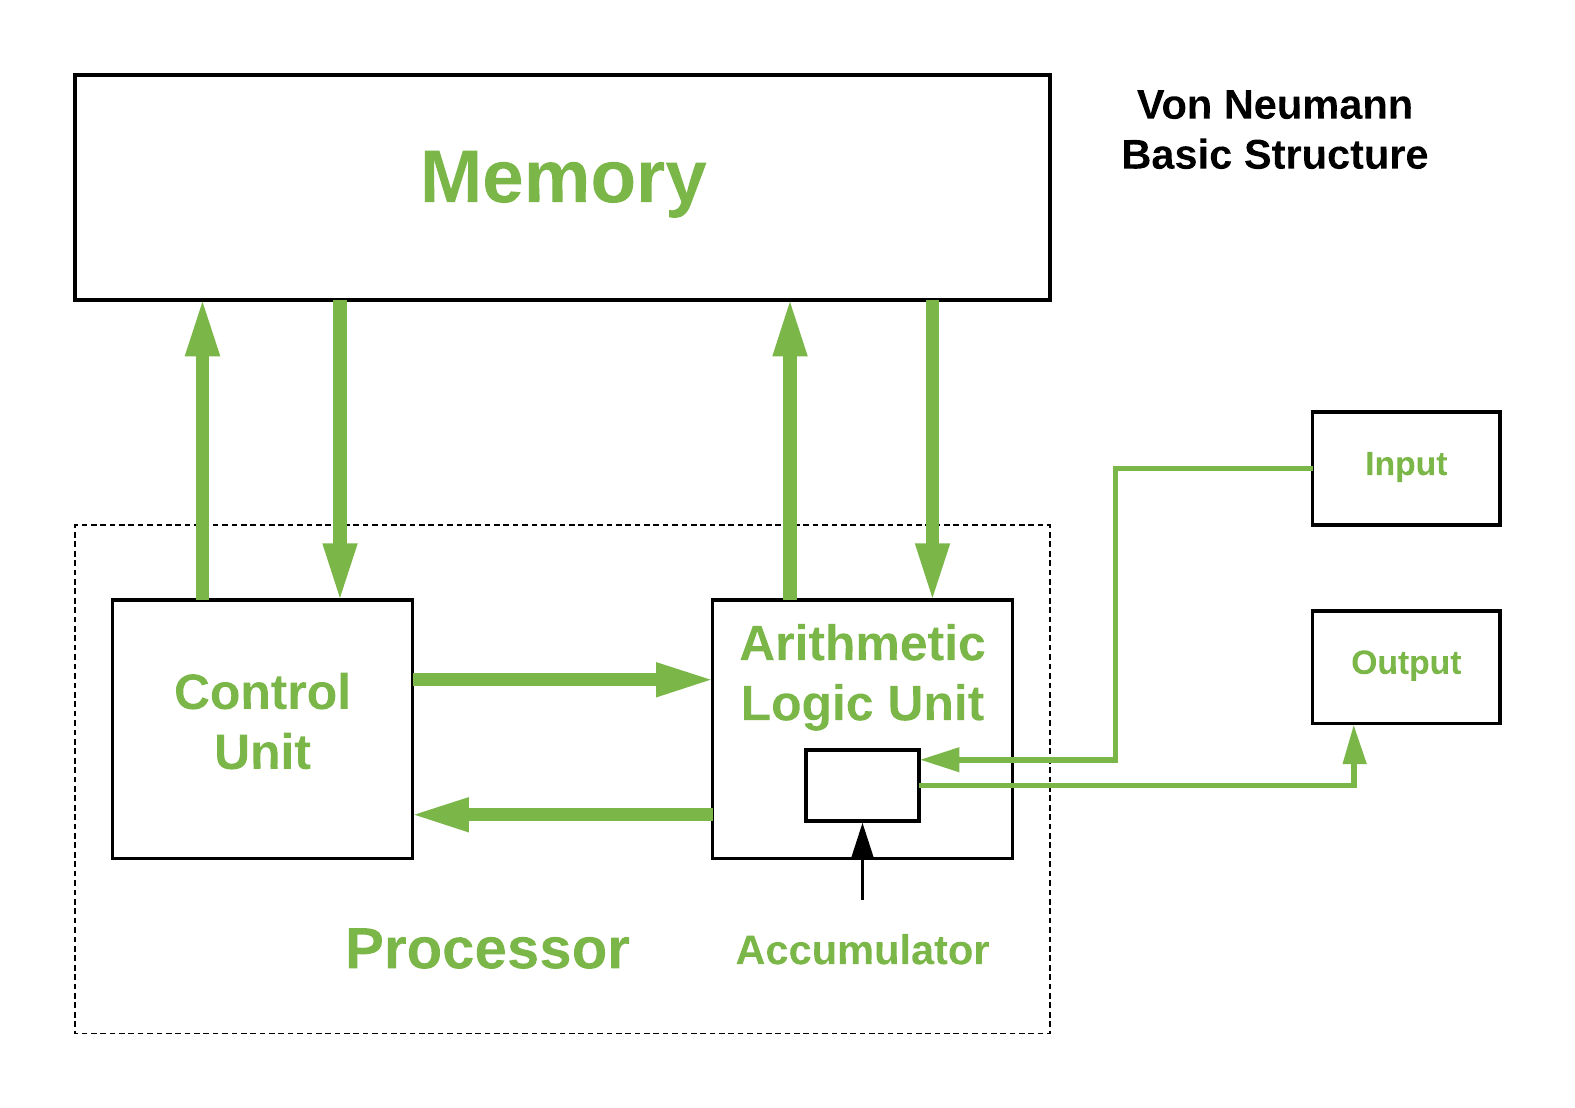
\includegraphics[width=0.5\textwidth,height=\textheight]{neumann.png}

Számítógép vásárlás szempontjából is alapvetően a CPU és a RAM határozza meg mennyire gyors a gép: minél nagyobb a CPU órajele (GHz) és minél több magja van, annál több utasítást tud végrehajtani a gép egy adott idő alatt, és minél nagyobb a RAM mérete (GB) annál több adatot tud egyszerre fejben tartani.
Talán nem ér minket meglepetésként, ha azt mondom, hogy a \emph{statisztikai számítások alapvetően RAM igényesek} (mert sok adattal dolgoznak). 16-32 GB már kell, hogy komolyabb statisztikai modelleket gyorsan tudjunk futtatni egy valós vállalati adattáblán (ami általában több, mint 1 millió rekroddal és minimum 30-40 oszloppal = változóval rendelkezik).

\section{A Pythonról általában}\label{a-pythonruxf3l-uxe1ltaluxe1ban}

Az Python a jegyzet írásakor a legnépszerűbb általános célú programozási nyelv, 2024 januárjában a \href{https://www.tiobe.com/tiobe-index/}{TIOBE index} alapján a legtöbb sor programkódot Python nyelven írják a fejlesztők.

A mi szempontunkból a Python olyan szempontból vonzó, hogy a külső kiegészítő csomagjai segítségével a valószínűségszámítás, statisztika és általánosabb adatelemzés műveletei könnyen és gyorsan elvégezhetők a segítségével. Tehát a Python használható olyan matematikai, statisztikai modellezési és elemzési feladatok elvégzésére alkalmas szkriptnyelvként, mint például az \href{https://cran.r-project.org/}{R} vagy a \href{https://www.mathworks.com/products/matlab.html}{Matlab}. A Python előnye ezekkel a nyelvekkel szemben, hogy mivel általános célú programnyelv, így a matematikai-statisztikai számítások eredményei sokkal könnyebben integrálhatók egy üzleti célú alkalmazásba, ami mondjuk felhasználói felülettel rendelkezik.
Ahogy az \emph{Előhang}ban már jeleztem, a jegyzet kimondottan a Python statisztikai és adatelemzési funkcióinak alapszintű bemutatásával foglalkozik. Tehát alkalmazást fejleszteni itt nem fogunk, a Pythont szkriptnyelvként működtetjük: elküldjük a programkódban megírt számítási igényeinket a gépállatnak, és az visszaköpi a számítások eredményeit a képernyőre, és mi egyrészt gyönyörködünk bennük, másrészt értelmezzük az eredményeket. Viszont, jó tudni, hogy a Python az eredmények további felhasználására is képes programnyelv. Ebben több, mint egy matematikusi körökben szintén népszerű R vagy Matlab. Hátránya a felsorolt nyelvekkel szemben, hogy mivel általános célú programnyelv, és nem kimondottan a matematikai-statisztikai számításokra optimalizált, így számos számítás lekódolása sokkal körülményesebb Pythonban, mint R-ben vagy Matlabban. De hát \emph{valamit valamiért}. :)

A Pythont, mi az \textbf{Anaconda keretrendszer}ből működtetjük, ami \href{https://www.anaconda.com/products/distribution}{innen letölthető}. Az Anaconda számos fejlesztőkörnyezetet biztosít a Python nyelvhez. Itt megjegyzendő, hogy a \textbf{Python és a Python fejlesztőkörnyezete nem összekeverendő!} A Python maga a programnyelv, amiben kódot írunk a számítógépünknek, hogy hajtsa végre, míg a fejlesztőkrönyezet az a program, amiben ezt a kódot megírjuk!
Mi a Python kódjainkat \textbf{Spyder fejlesztőkörnyezetben} írjuk majd, mivel ez a fejlesztőkörnyezet az, ami leginkább a Python matematikai-statisztikai műveleteket végrehajtó, szkriptnyelv-szerű használatára van optimalizálva.

Miután telepítettük és elindítottuk az Anaconda keretrendszert, a kezdőképernyőről rögtön indíthatjuk is a Spydert:


\includegraphics[width=0.8\textwidth,height=\textheight]{Anaconda.jpg}

\section{A Spyder felülete}\label{a-spyder-feluxfclete}

A Spyder fejlesztőkörnyezet indítása után az alábbihoz hasonló képernyőkép fogad minket:

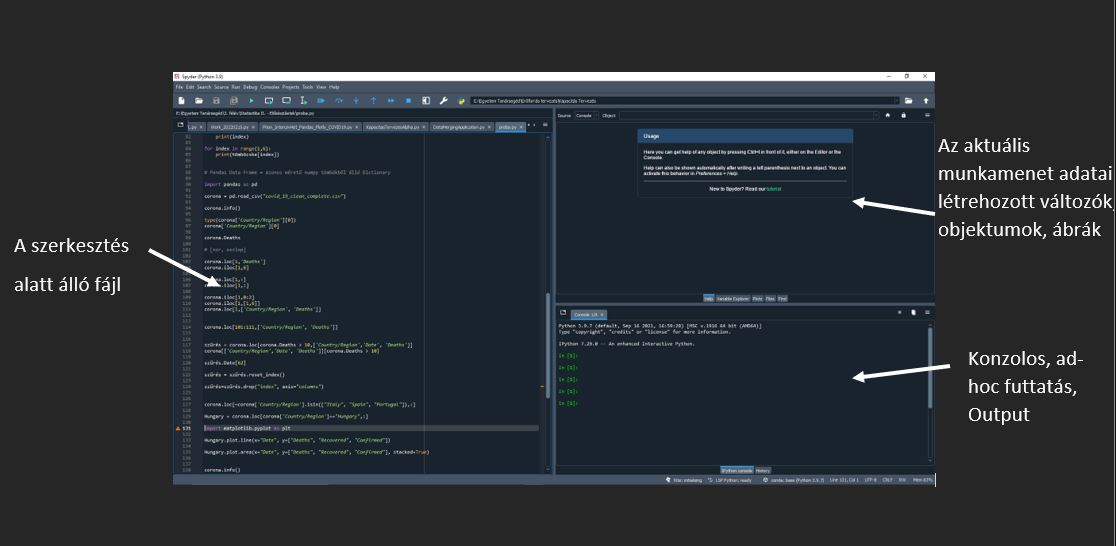
\includegraphics[width=0.9\textwidth,height=\textheight]{Spyder.jpg}

A Python kódokat a Spyder-ben \emph{.py} kiterjesztésű szkriptfájokban fogjuk írni.
Egy ilyet az alább látható módon lehet létrehozni:

A szkriptfájlba írhatjuk a gépállatnak szóló utasításainkat Python nyelven. Az utasítások végrehajtását a Spyder felület felső részén lakó 
\includegraphics{RunLine.jpg} gomb megtaposásával tudjuk kérni a géptől, aki az utasítás eredményét alul, a \emph{Console} felületen köpi ki. Ekkor a Spyder mindig azt a Python utasítást hajtja végre a gomb megnyomásakor, amiben éppen a villogó kurzorral álltunk.
Egy példában számoltassuk ki a Pythonnal, hogy mennyi \(3+2\):

Több utasítást is végre tudunk hajtatni a géppel egyszerre. Csak jelöljük ki a szkriptben a végrehajtandó utasításokat, és így kijelölés után tapossuk meg a Spyíder felső menüsorában található 
\includegraphics{RunLine.jpg} gombot!
Egy utasítást több sorba is írhatunk, de egy új utasítás mindig új sorban kezdődjön! Érdemes egy üres sort is hagyni az előző utasítás vége után!

Számoltassunk akkor most ki a Pythonnal egyszerre két dolgot is: mennyi \(3+2\) és mennyi \(3 \times 2\):

Ezek után a jegyezetek további részében a feladatok elvégzéséhez szükséges Python kódrészleteket és azok eredményét az alábbi módon jelölöm:

\begin{Shaded}
\begin{Highlighting}[]
\DecValTok{3}\OperatorTok{+}\DecValTok{2}
\end{Highlighting}
\end{Shaded}

\begin{verbatim}
## 5
\end{verbatim}

\begin{Shaded}
\begin{Highlighting}[]
\DecValTok{3}\OperatorTok{*}\DecValTok{2}
\end{Highlighting}
\end{Shaded}

\begin{verbatim}
## 6
\end{verbatim}

Ha az összes \emph{.py} fájlukban lévő kódot le szeretnénk futtatni abban a sorrendben, ahogy a fájlban szerepelnek, akkor a Spyder felső menüsorán a 
\includegraphics{RunFile.jpg} gombot kell megütni. De vigyázzunk, ilyenkor a Python nem írja ki az utasításaink eredményét a konzolra, csak akkor, ha külön beágyazzuk őket egy \texttt{print} nevű extra utasítás zárójelei közé!

\begin{Shaded}
\begin{Highlighting}[]
\BuiltInTok{print}\NormalTok{(}\DecValTok{3}\OperatorTok{+}\DecValTok{2}\NormalTok{)}
\end{Highlighting}
\end{Shaded}

\begin{verbatim}
## 5
\end{verbatim}

\begin{Shaded}
\begin{Highlighting}[]
\BuiltInTok{print}\NormalTok{(}\DecValTok{3}\OperatorTok{*}\DecValTok{2}\NormalTok{)}
\end{Highlighting}
\end{Shaded}

\begin{verbatim}
## 6
\end{verbatim}

A művelet videón:

\section{Working Directory}\label{working-directory}

Mielőtt belevágunk a Python mélyebb rejtelmeibe van még egy fontos dolog, amiről még szót kell ejteni: a \emph{Working Directory} kérdéséről.
A \emph{Working Directory} az a mappa, ahonnan a \emph{pitonállat} alapértelmezés szerint minden fájlt innen akar a memóriába tölteni és ide akar visszaírni.
A Spyder jobb felső sarkában lévő részen lehet kiválasztani és beállítani, hogy melyik mappa legyen a \emph{Working Directory}. Ezek után \textbf{minden fájlunk alapból ide fog mentődni, és minden adattáblát ide rakjunk be, amivel majd a Pythonban dolgozni akarunk!}

A Spyder-ben alapértelmezett \emph{Working Directory}-t is be tudunk állítani, ha elbandukolunk a \textbf{Tools --\textgreater{} Preferences --\textgreater{} Current working directory} menübe, és ott a \textbf{Console directory / The following directory} című résznél beállítjuk a kívánt fix mappát alapértelmezett \emph{Working Directory}-nak.

Az egész alapértelmezett \emph{Working Directory}-val kapcsolatos okfejtés működésben megnézhető a következő videón:

\section{Alapvető Python adattípusok és adatszerkezetek}\label{alapvetux151-python-adattuxedpusok-uxe9s-adatszerkezetek}

Eddig a Pythonban csak utasításokat hajtattunk végre, de a memóriában (RAM-ban) nem tároltattunk el még vele semmit.
Most itt az idő! Az utasítások eredményét a \texttt{=} szimbólummal tudjuk a memóriába valamilyen szimpatikus néven elmenteni.

\subsection{Egyszerű adattípusok}\label{egyszerux171-adattuxedpusok}

Mentsük el a 3+2 eredményét egy \texttt{összeg} névre hallgató R objektumba: \texttt{összeg\ =\ 3+2}. Az utasítás végrehajtásának hatására az \texttt{összeg} objektum megjelenik az Spyder \emph{jobb felső} sarkában lévő résznél, a \emph{Variable Explorer} fülön. (A Python alapjáraton karakterkészletben elég bő, így simán tudunk ékezetes objektumneveket is adni. De néha én a biztonság kedvéért megmaradok az ékezet nélküli elnevezéseknél. Öreg vagyok már, na! :)). A Spyder képernyőnek ezen a \emph{Variable Explorer} részén látjuk mindig azt, hogy éppen milyen Python objektumok élnek a RAM-ban:

A Python memória-objektumoknak több fajtája van. A legegyszerűbbek azok, amik csak egy értéket tartalmaznak (mint nekünk az előbb az \texttt{osszeg}). Ezeket szokás \textbf{változó}nak is hívni. Én nem szeretem ezt az elnevezést, mert keverhető a statisztikai értelemben vett változóval, ami mindig egy statisztikai megfigyelést leíró tulajdonságot/ismérvet jelent (pl. munkavállaló jövdeleme). Ennek ellenére én is gyakran használom a Python memória objektumokra a változó elnevezést. :)

A Python objektumoknak mindig van \textbf{adattípusa} is, ami \textbf{leírja, hogy az adott objektumban számértékű, szöveges, dátum vagy valami egyéb jellegű adatot tárolunk-e}. Ez azért marha fontos, mert az adattípustól függ, hogy mennyi hely szükséges a RAM-ban az objektum tárolásához. Érzésre megmondható talán, hogy egy szöveges adat tárolására több hely kell, mint egy egész szám tárolásához.

Az adattípusokat Pythonban a \texttt{type} névre hallgató \textbf{beépített függvénnyel} lehet lekérdezni.

Ezen a ponton érdemes megemlékezni arról, hogy a Pythonban léteznek \textbf{függvényként működő beépített utasítások} is. Ezek az úgynevezett Python függvények olyan utasítások, amik a matekban megszokott \(f(x)\) függvény alakot veszik fel.
A függvény neve leírja, hogy a függvény milyen műveletet végeztet el a gépállattal, és a zárójelek között pedig megadjuk, hogy milyen bemeneti paramétereken (adatokon) kell elvégezni a kijelölt műveletet. Pl. ilyen függvény volt már a \texttt{print} is.

Gyakorlati példaként lássuk akkor \textbf{Python függvények}re a \texttt{type} működését:

\begin{Shaded}
\begin{Highlighting}[]
\NormalTok{összeg }\OperatorTok{=} \DecValTok{3}\OperatorTok{+}\DecValTok{2}
\BuiltInTok{type}\NormalTok{(összeg)}
\end{Highlighting}
\end{Shaded}

\begin{verbatim}
## <class 'int'>
\end{verbatim}

Ez a \texttt{type} nevű jószág azt csiripeli nekünk, hogy ez az \texttt{összeg} című változó egy \texttt{int} adattípusú, azaz \textbf{egész szám}, leánykori angolos nevén \texttt{integer}. Tehát, ha egy Python objektum \texttt{int} adattípusú, akkor az azt jelenti, hogy ő bezony csak egész számokat tud elképzelni a világban, tört számokat nem tud tárolni.

Törtszámok tárolására vannak a \texttt{float} adattípusú objektumok.

\begin{Shaded}
\begin{Highlighting}[]
\NormalTok{tört }\OperatorTok{=} \DecValTok{3}\OperatorTok{/}\DecValTok{2}
\BuiltInTok{type}\NormalTok{(tört)}
\end{Highlighting}
\end{Shaded}

\begin{verbatim}
## <class 'float'>
\end{verbatim}

A Statisztika II. tárgyban a kétféle számítpus közti különbségnek nem igazán lesz jelentősége, de ha igazi \emph{big data}-val foglalkozik az ember, akkor a RAM takarékosság miatt számít, hogy valami csak egy egész számnyi, vagy egy törtszámnyi helyet foglal sok-sok tizedeshellyel!

Néhány egyéb fontosabb adattípus és megadási módjuk:

\begin{Shaded}
\begin{Highlighting}[]
\NormalTok{szoveg }\OperatorTok{=} \StringTok{"Hello There!"} \CommentTok{\# Figyeljünk rá, hogy szöveget a kódban csak idézőjelek közé rakjunk! Mint Excelben! :)}
\BuiltInTok{type}\NormalTok{(szoveg)}
\end{Highlighting}
\end{Shaded}

\begin{verbatim}
## <class 'str'>
\end{verbatim}

\begin{Shaded}
\begin{Highlighting}[]
\NormalTok{igazhamis }\OperatorTok{=} \VariableTok{True}
\BuiltInTok{type}\NormalTok{(igazhamis) }\CommentTok{\# a bool típusnak csak két értéke lehet: True vagy False}
\end{Highlighting}
\end{Shaded}

\begin{verbatim}
## <class 'bool'>
\end{verbatim}

A fenti kódrészletben szereplő \textbf{\#} jel a komment jele a Pythonban. A \textbf{\#} mögötti részeket a gépállat nem fogja végrehajtani, olyan lesz neki, mintha ott sem lenne. Ezzel magunknak írhatunk a Python szkriptbe hasznos megjegyzéseket.

Az egyes adattípusok között tudunk konvertálni, ha van ennek van értelme. A konverzóra függvényeket tudunk használni, amik neve kivétel nélkül megegyezik azzal a kulcsszóval, amit a \texttt{type} függvény visszaad adattípusnak. Tehát a függvény, ami mondjuk az objektumot szöveggé, azaz stringgé konvertálja az \texttt{str} névre hallgat.

Tehát akkor számból tudunk szöveget csinálni:

\begin{Shaded}
\begin{Highlighting}[]
\NormalTok{szam }\OperatorTok{=} \DecValTok{1992}
\BuiltInTok{type}\NormalTok{(szam)}
\end{Highlighting}
\end{Shaded}

\begin{verbatim}
## <class 'int'>
\end{verbatim}

\begin{Shaded}
\begin{Highlighting}[]
\NormalTok{nemszam }\OperatorTok{=} \BuiltInTok{str}\NormalTok{(szam)}
\BuiltInTok{type}\NormalTok{(nemszam)}
\end{Highlighting}
\end{Shaded}

\begin{verbatim}
## <class 'str'>
\end{verbatim}

\begin{Shaded}
\begin{Highlighting}[]
\NormalTok{nemszam}
\end{Highlighting}
\end{Shaded}

\begin{verbatim}
## '1992'
\end{verbatim}

Láthjatjuk, hogy amikor kiíratjuk a \texttt{nemszam} változót, akkor ott az \(1992\) már aposztrófok között van, ami azt jelöli, hogy ez beza már szöveges, azaz \emph{string} adat.

Olyan szövegből tudunk számot csinálni, aminek tartalma tényleg egy valid szám:

\begin{Shaded}
\begin{Highlighting}[]
\NormalTok{szöveg }\OperatorTok{=} \StringTok{"1992"}
\BuiltInTok{type}\NormalTok{(szöveg)}
\end{Highlighting}
\end{Shaded}

\begin{verbatim}
## <class 'str'>
\end{verbatim}

\begin{Shaded}
\begin{Highlighting}[]
\NormalTok{nemszöveg }\OperatorTok{=} \BuiltInTok{int}\NormalTok{(szöveg)}
\BuiltInTok{type}\NormalTok{(nemszöveg)}
\end{Highlighting}
\end{Shaded}

\begin{verbatim}
## <class 'int'>
\end{verbatim}

Tizedestörtekkel vigyázzunk! A \textbf{Python angol lokalizációt feltételez mindig}, így tizedes pontot kell alkalmazni! A tizedes vesszővel írt számot nem fogja felismerni, és hisztis hibaüzenetet dob. :( A \texttt{nemjo} változó pedig nem jön létre a memóriában.

\begin{Shaded}
\begin{Highlighting}[]
\NormalTok{nemjo }\OperatorTok{=} \BuiltInTok{float}\NormalTok{(}\StringTok{"3,14"}\NormalTok{)}
\end{Highlighting}
\end{Shaded}

\begin{verbatim}
## ValueError: could not convert string to float: '3,14'
\end{verbatim}

\begin{Shaded}
\begin{Highlighting}[]
\NormalTok{nemjo}
\end{Highlighting}
\end{Shaded}

\begin{verbatim}
## NameError: name 'nemjo' is not defined
\end{verbatim}

\begin{Shaded}
\begin{Highlighting}[]
\BuiltInTok{type}\NormalTok{(nemjo)}
\end{Highlighting}
\end{Shaded}

\begin{verbatim}
## NameError: name 'nemjo' is not defined
\end{verbatim}

De ha a törtszám tizedes ponttal adott a string változóban, akkor az minden további nélkül \texttt{float} adattípusra konvertálható.

\begin{Shaded}
\begin{Highlighting}[]
\NormalTok{jo }\OperatorTok{=} \BuiltInTok{float}\NormalTok{(}\StringTok{"3.14"}\NormalTok{)}
\NormalTok{jo}
\end{Highlighting}
\end{Shaded}

\begin{verbatim}
## 3.14
\end{verbatim}

\begin{Shaded}
\begin{Highlighting}[]
\BuiltInTok{type}\NormalTok{(jo)}
\end{Highlighting}
\end{Shaded}

\begin{verbatim}
## <class 'float'>
\end{verbatim}

Ha törtszámot (\texttt{float}) etetünk meg vacsorára az \texttt{int} függvénnyel, akkor annak az egészrészét veszi.

\begin{Shaded}
\begin{Highlighting}[]
\NormalTok{fura }\OperatorTok{=} \BuiltInTok{int}\NormalTok{(}\FloatTok{3.14}\NormalTok{)}
\NormalTok{fura}
\end{Highlighting}
\end{Shaded}

\begin{verbatim}
## 3
\end{verbatim}

\begin{Shaded}
\begin{Highlighting}[]
\BuiltInTok{type}\NormalTok{(fura)}
\end{Highlighting}
\end{Shaded}

\begin{verbatim}
## <class 'int'>
\end{verbatim}

Pythonban a rosszul beállított adattípusokból születhet pár baleset. Íme a leggyakoribb példák.

A \texttt{+} két string között az összefűzést jelenti, így az alábbi kód tökéletesen működőképes.

\begin{Shaded}
\begin{Highlighting}[]
\NormalTok{szoveg1 }\OperatorTok{=} \StringTok{"Hello"}
\NormalTok{szoveg2 }\OperatorTok{=} \StringTok{"There"}

\NormalTok{szoveg1}\OperatorTok{+}\NormalTok{szoveg2}
\end{Highlighting}
\end{Shaded}

\begin{verbatim}
## 'HelloThere'
\end{verbatim}

Viszont a string és integer összege nem értelmezhető, így hibaüzi lesz a vége\ldots mily meglepő :)
Ellenben a szorzatuk értelmes eredményt mutat: a stringet összefűzi annyiszor amennyi az integer típusú változó értéke!

\begin{Shaded}
\begin{Highlighting}[]
\NormalTok{szoveg }\OperatorTok{=} \StringTok{"3"}
\NormalTok{szam }\OperatorTok{=} \DecValTok{4}

\NormalTok{szoveg}\OperatorTok{+}\NormalTok{szam}
\end{Highlighting}
\end{Shaded}

\begin{verbatim}
## TypeError: can only concatenate str (not "int") to str
\end{verbatim}

\begin{Shaded}
\begin{Highlighting}[]
\NormalTok{szoveg}\OperatorTok{*}\NormalTok{szam}
\end{Highlighting}
\end{Shaded}

\begin{verbatim}
## '3333'
\end{verbatim}

Érdemes megnézni mi történik, ha egy stringként tárolt egész számot és egy integerként tárolt egész számot úgy ``adunk össze'' és ``szorzunk össze'', hogy előtte a stringet integerré, vagy floattá konvertáljuk.

\begin{Shaded}
\begin{Highlighting}[]
\NormalTok{szoveg }\OperatorTok{=} \StringTok{"3"}
\NormalTok{szam }\OperatorTok{=} \DecValTok{4}

\BuiltInTok{int}\NormalTok{(szoveg)}\OperatorTok{+}\NormalTok{szam}
\end{Highlighting}
\end{Shaded}

\begin{verbatim}
## 7
\end{verbatim}

\begin{Shaded}
\begin{Highlighting}[]
\BuiltInTok{int}\NormalTok{(szoveg)}\OperatorTok{*}\NormalTok{szam}
\end{Highlighting}
\end{Shaded}

\begin{verbatim}
## 12
\end{verbatim}

\begin{Shaded}
\begin{Highlighting}[]
\BuiltInTok{float}\NormalTok{(szoveg)}\OperatorTok{+}\NormalTok{szam}
\end{Highlighting}
\end{Shaded}

\begin{verbatim}
## 7.0
\end{verbatim}

\begin{Shaded}
\begin{Highlighting}[]
\BuiltInTok{float}\NormalTok{(szoveg)}\OperatorTok{*}\NormalTok{szam}
\end{Highlighting}
\end{Shaded}

\begin{verbatim}
## 12.0
\end{verbatim}

Ekkor igazából semmi galiba nem történik, minden szituáció értelmes eredményre vezet. Annyi, hogy amikor \texttt{float}-ra konvertáltuk a stringben tárolt egész számot, akkor az eredmény is \texttt{float} típusú objektum lesz. Ezt onnan látni a \texttt{type} függvény nélkül, hogy pl. a \texttt{float(szoveg)+szam} eredménye \(7.0\) lesz a \texttt{int(szoveg)+szam}-féle \(7\) helyett.

Viszont, ha a stringben egy tizedes törtet tárolok el (rendesen tizedes ponttal), akkor az már összeveszik az \texttt{int} függvénnyel, és ezekben a csillagálásokban hibát dob a pitonállat.

\begin{Shaded}
\begin{Highlighting}[]
\NormalTok{szoveg }\OperatorTok{=} \StringTok{"3.5"}
\NormalTok{szam }\OperatorTok{=} \DecValTok{4}

\NormalTok{szoveg}\OperatorTok{+}\NormalTok{szam}
\end{Highlighting}
\end{Shaded}

\begin{verbatim}
## TypeError: can only concatenate str (not "int") to str
\end{verbatim}

\begin{Shaded}
\begin{Highlighting}[]
\NormalTok{szoveg}\OperatorTok{*}\NormalTok{szam}
\end{Highlighting}
\end{Shaded}

\begin{verbatim}
## '3.53.53.53.5'
\end{verbatim}

\begin{Shaded}
\begin{Highlighting}[]
\BuiltInTok{int}\NormalTok{(szoveg)}\OperatorTok{+}\NormalTok{szam}
\end{Highlighting}
\end{Shaded}

\begin{verbatim}
## ValueError: invalid literal for int() with base 10: '3.5'
\end{verbatim}

\begin{Shaded}
\begin{Highlighting}[]
\BuiltInTok{int}\NormalTok{(szoveg)}\OperatorTok{*}\NormalTok{szam}
\end{Highlighting}
\end{Shaded}

\begin{verbatim}
## ValueError: invalid literal for int() with base 10: '3.5'
\end{verbatim}

\begin{Shaded}
\begin{Highlighting}[]
\BuiltInTok{float}\NormalTok{(szoveg)}\OperatorTok{+}\NormalTok{szam}
\end{Highlighting}
\end{Shaded}

\begin{verbatim}
## 7.5
\end{verbatim}

\begin{Shaded}
\begin{Highlighting}[]
\BuiltInTok{float}\NormalTok{(szoveg)}\OperatorTok{*}\NormalTok{szam}
\end{Highlighting}
\end{Shaded}

\begin{verbatim}
## 14.0
\end{verbatim}

Ha egészrészt szeretnék venni a stringként tárolt törtszámomból, akkor az \texttt{int} alkalmazása előtt beza \texttt{float}-tá kell konvertálni.

\begin{Shaded}
\begin{Highlighting}[]
\NormalTok{szoveg }\OperatorTok{=} \StringTok{"3.5"}
\NormalTok{szam }\OperatorTok{=} \DecValTok{4}

\NormalTok{szoveg}\OperatorTok{+}\NormalTok{szam}
\end{Highlighting}
\end{Shaded}

\begin{verbatim}
## TypeError: can only concatenate str (not "int") to str
\end{verbatim}

\begin{Shaded}
\begin{Highlighting}[]
\NormalTok{szoveg}\OperatorTok{*}\NormalTok{szam}
\end{Highlighting}
\end{Shaded}

\begin{verbatim}
## '3.53.53.53.5'
\end{verbatim}

\begin{Shaded}
\begin{Highlighting}[]
\BuiltInTok{int}\NormalTok{(}\BuiltInTok{float}\NormalTok{(szoveg))}\OperatorTok{+}\NormalTok{szam}
\end{Highlighting}
\end{Shaded}

\begin{verbatim}
## 7
\end{verbatim}

\begin{Shaded}
\begin{Highlighting}[]
\BuiltInTok{int}\NormalTok{(}\BuiltInTok{float}\NormalTok{(szoveg))}\OperatorTok{*}\NormalTok{szam}
\end{Highlighting}
\end{Shaded}

\begin{verbatim}
## 12
\end{verbatim}

\begin{Shaded}
\begin{Highlighting}[]
\BuiltInTok{float}\NormalTok{(szoveg)}\OperatorTok{+}\NormalTok{szam}
\end{Highlighting}
\end{Shaded}

\begin{verbatim}
## 7.5
\end{verbatim}

\begin{Shaded}
\begin{Highlighting}[]
\BuiltInTok{float}\NormalTok{(szoveg)}\OperatorTok{*}\NormalTok{szam}
\end{Highlighting}
\end{Shaded}

\begin{verbatim}
## 14.0
\end{verbatim}

\subsection{Összetett adatszerkezetek}\label{uxf6sszetett-adatszerkezetek}

\subsubsection{\texorpdfstring{A Python \texttt{list}}{A Python list}}\label{a-python-list}

Egyszerre több értéket tartalmazó objektumot is fel tudunk venni a Python memóriájába, ha \texttt{{[}{]}} zárójelek között vesszővel felsoroljuk az eltárolandó értékeket. Ennek az objektumnak a neve \texttt{list}.

\begin{Shaded}
\begin{Highlighting}[]
\NormalTok{sokszam }\OperatorTok{=}\NormalTok{ [}\FloatTok{3.14}\NormalTok{, }\FloatTok{2.71}\NormalTok{, }\DecValTok{88}\NormalTok{, }\DecValTok{1234}\NormalTok{]}
\BuiltInTok{type}\NormalTok{(sokszam)}
\end{Highlighting}
\end{Shaded}

\begin{verbatim}
## <class 'list'>
\end{verbatim}

Írassuk ki a teljes listát egyben az outputra!

\begin{Shaded}
\begin{Highlighting}[]
\NormalTok{sokszam}
\end{Highlighting}
\end{Shaded}

\begin{verbatim}
## [3.14, 2.71, 88, 1234]
\end{verbatim}

Kérjük le a lista \(1.\) és \(3.\) elemeit! Egy elemet a listából a sorszámával tudunk kinyerni, ha ezt a sorszámot \texttt{{[}{]}} zárójelek között megadjuk. Ugyanakkor figyeljünk, hogy a Pitonállat \(0\)-tól indexel! Azaz, az 1. elem a 0.; 2. az 1.; 3. a 2. és stb.

\begin{Shaded}
\begin{Highlighting}[]
\NormalTok{sokszam[}\DecValTok{0}\NormalTok{]}
\end{Highlighting}
\end{Shaded}

\begin{verbatim}
## 3.14
\end{verbatim}

\begin{Shaded}
\begin{Highlighting}[]
\NormalTok{sokszam[}\DecValTok{2}\NormalTok{]}
\end{Highlighting}
\end{Shaded}

\begin{verbatim}
## 88
\end{verbatim}

Nézzük meg az adattípusait is ezeknek a listaelemeknek.

\begin{Shaded}
\begin{Highlighting}[]
\BuiltInTok{type}\NormalTok{(sokszam[}\DecValTok{0}\NormalTok{])}
\end{Highlighting}
\end{Shaded}

\begin{verbatim}
## <class 'float'>
\end{verbatim}

\begin{Shaded}
\begin{Highlighting}[]
\BuiltInTok{type}\NormalTok{(sokszam[}\DecValTok{2}\NormalTok{])}
\end{Highlighting}
\end{Shaded}

\begin{verbatim}
## <class 'int'>
\end{verbatim}

Láthatjuk, hogy a lista megőrzi az elemeinek eredeti adattípusát. Tehát, a \(3.14\) adattípusa \texttt{float}, míg a \(88\)-é \texttt{int}. Ezzel sokat spórol a memóriánkon, hogy nem kényszeríti át a \(88\)-at is \texttt{float}-ba az egységesség jegyében.

Ez a logika szövegekkel is működik. Ha felveszek egy szöveges értéket is a listába, akkor annak az adattípusa string, azaz \texttt{str} lesz. A számértékű adatok pedig maradnak annak rendje és módja szerint \texttt{float} és \texttt{int} típusban, ami éppen kell. :)

\begin{Shaded}
\begin{Highlighting}[]
\NormalTok{sokszam\_sokszoveg }\OperatorTok{=}\NormalTok{ [}\DecValTok{88}\NormalTok{, }\DecValTok{42}\NormalTok{, }\StringTok{"Hello"}\NormalTok{, }\DecValTok{1992}\NormalTok{, }\DecValTok{9}\NormalTok{, }\StringTok{"There"}\NormalTok{, }\StringTok{"Friend"}\NormalTok{, }\DecValTok{11}\NormalTok{]}

\BuiltInTok{type}\NormalTok{(sokszam\_sokszoveg[}\DecValTok{0}\NormalTok{])}
\end{Highlighting}
\end{Shaded}

\begin{verbatim}
## <class 'int'>
\end{verbatim}

\begin{Shaded}
\begin{Highlighting}[]
\BuiltInTok{type}\NormalTok{(sokszam\_sokszoveg[}\DecValTok{2}\NormalTok{])}
\end{Highlighting}
\end{Shaded}

\begin{verbatim}
## <class 'str'>
\end{verbatim}

Kérjük le, hogy egy lista hány elemet tartalmaz. Ezt a \texttt{len} nevű függvény intézi nekünk.

\begin{Shaded}
\begin{Highlighting}[]
\BuiltInTok{len}\NormalTok{(sokszam\_sokszoveg)}
\end{Highlighting}
\end{Shaded}

\begin{verbatim}
## 8
\end{verbatim}

8 elemű a lista, szupszi!

Viszont, ezt az elemszám lekérdezést meg lehet oldani úgynevezett \textbf{metódus} segítségével is! A \textbf{metódusok olyan függvények, amik egy konkrét memóriában élő objektumon hajtanak végre műveleteket}. Ez a spéci logika a Python nyelvben úgy jelenik meg, hogy \textbf{nem azt mondjuk}, hogy \(f(x)\) módon végrehajtom az \(f\) műveletet az \(x\) objektumon. Mint ahogy a \texttt{len(sokszam\_sokszoveg)} is működik, **hanem úgy gondolkodunk, hogy \(x.f()\) módon végrehajtjuk az \(x\) objektumon az \(f\) műveletet.
Ez a gyakorlatban a \texttt{sokszam\_sokszoveg} nevű lista elemszámának lekérdezésénél az alábbi módon működik.

\begin{Shaded}
\begin{Highlighting}[]
\NormalTok{sokszam\_sokszoveg.}\FunctionTok{\_\_len\_\_}\NormalTok{()}
\end{Highlighting}
\end{Shaded}

\begin{verbatim}
## 8
\end{verbatim}

Királyság, az eredmény így is tök \(8\). :) A legtöbb metódus nevében amúgy nincsenek ilyen hosszas \texttt{\_\_} részek. Illetve, a metódusok zárójelei közé lehet majd egyéb paramétereket is írni, amik szabályozzák a metódus működését. Ilyen például a lista elemeinek sorbarendezési művelete.

Egy listát sorba rendezni ugyanis már csak metódussal tudunk, ami \texttt{sort} néven fut. Ezt kell elsütni a listánkon egy kis pontocskával megtámogatva.

\begin{Shaded}
\begin{Highlighting}[]
\NormalTok{sokszam.sort()}
\NormalTok{sokszam}
\end{Highlighting}
\end{Shaded}

\begin{verbatim}
## [2.71, 3.14, 88, 1234]
\end{verbatim}

Szépen növekvő sorban vannak már itt a számaink. Viszont BRÉKÓ van, mert a \texttt{sort} metódus \textbf{felülírta az eredeti listát, tehát az értékek eredeti sorrendje elveszett!} Ha \textbf{szükségünk van az eredeti sorrendre}, akkor beza \textbf{másolatot kell készíteni az eredeti listából a rendezés előtt!} Ezt a másolat készítést a \texttt{copy} metódussal tudjuk megtenni. Ha ezt nem alkalmazzuk, akkor a gépállat olyan szinten kezeli az új objektumot is, hogy mindent megcsinál vele, amit az eredetivel! Ha ezt a kapcsolatot a másolat és az eredeti objektum között \emph{el akarjuk vágni}, akkor kell a \texttt{copy} metódus.

\begin{Shaded}
\begin{Highlighting}[]
\NormalTok{sokszam }\OperatorTok{=}\NormalTok{ [}\FloatTok{3.14}\NormalTok{, }\FloatTok{2.71}\NormalTok{, }\DecValTok{1234}\NormalTok{, }\DecValTok{88}\NormalTok{]}
\NormalTok{sokszam\_copy }\OperatorTok{=}\NormalTok{ sokszam.copy()}
\NormalTok{sokszam.sort()}
\NormalTok{sokszam}
\end{Highlighting}
\end{Shaded}

\begin{verbatim}
## [2.71, 3.14, 88, 1234]
\end{verbatim}

\begin{Shaded}
\begin{Highlighting}[]
\NormalTok{sokszam\_copy}
\end{Highlighting}
\end{Shaded}

\begin{verbatim}
## [3.14, 2.71, 1234, 88]
\end{verbatim}

Láthatjuk, hogy a fenti példában minden oké, megvan az eredeti sorrend is a \texttt{sokszam\_copy}-ban. De itt lentebb, ha lehagyom a \texttt{copy}-t, akkor GázGéza van!

\begin{Shaded}
\begin{Highlighting}[]
\NormalTok{sokszam }\OperatorTok{=}\NormalTok{ [}\FloatTok{3.14}\NormalTok{, }\FloatTok{2.71}\NormalTok{, }\DecValTok{1234}\NormalTok{, }\DecValTok{88}\NormalTok{]}
\NormalTok{sokszam\_copy }\OperatorTok{=}\NormalTok{ sokszam}
\NormalTok{sokszam.sort()}
\NormalTok{sokszam}
\end{Highlighting}
\end{Shaded}

\begin{verbatim}
## [2.71, 3.14, 88, 1234]
\end{verbatim}

\begin{Shaded}
\begin{Highlighting}[]
\NormalTok{sokszam\_copy}
\end{Highlighting}
\end{Shaded}

\begin{verbatim}
## [2.71, 3.14, 88, 1234]
\end{verbatim}

Viszont, ha csökkenő és nem növekvő sorrendet akarok a listában, akkor azt a \texttt{sort} metódus zárójelei között, \textbf{paraméterként tudom megadni} \texttt{reverse=True} módon.

\begin{Shaded}
\begin{Highlighting}[]
\NormalTok{sokszam.sort(reverse}\OperatorTok{=}\VariableTok{True}\NormalTok{)}
\NormalTok{sokszam}
\end{Highlighting}
\end{Shaded}

\begin{verbatim}
## [1234, 88, 3.14, 2.71]
\end{verbatim}

Oké, ez működik! :) Azt, hogy egy metódusnak vagy általános függvénynek milyen paraméterei vannak, azt pl. a Python nyelv \href{https://www.w3schools.com/python/ref_list_sort.asp}{w3schools-on található online dokumentációjából} lehet kideríteni. Itt a metódus/függvény nevére kell rákeresni.
Szép szóval azt szokás mondani, hogy a dokumentáció megadja, hogy az egyes Python függvényeket milyen paraméterezéssel (más néven argumentumokkal) lehet \emph{meghívni}.

A sorbarendezés működik csak stringeket tartalmazó listára is.

\begin{Shaded}
\begin{Highlighting}[]
\NormalTok{soknév }\OperatorTok{=}\NormalTok{ [}\StringTok{"Kovács"}\NormalTok{, }\StringTok{"László"}\NormalTok{, }\StringTok{"Balázsné"}\NormalTok{, }\StringTok{"Mócsai"}\NormalTok{, }\StringTok{"Andrea"}\NormalTok{, }\StringTok{"Musa"}\NormalTok{]}

\NormalTok{soknév.sort()}
\NormalTok{soknév}
\end{Highlighting}
\end{Shaded}

\begin{verbatim}
## ['Andrea', 'Balázsné', 'Kovács', 'László', 'Musa', 'Mócsai']
\end{verbatim}

\begin{Shaded}
\begin{Highlighting}[]
\NormalTok{soknév.sort(reverse}\OperatorTok{=}\VariableTok{True}\NormalTok{)}
\NormalTok{soknév}
\end{Highlighting}
\end{Shaded}

\begin{verbatim}
## ['Mócsai', 'Musa', 'László', 'Kovács', 'Balázsné', 'Andrea']
\end{verbatim}

Ellenben, ha a listában vegyesen vannak stringek és valami számértéket jelölő adattípusok (\texttt{int} és \texttt{float}), akkor a rendezés vége egy szép kis hibaüzenet lesz.

\begin{Shaded}
\begin{Highlighting}[]
\NormalTok{sokszam\_sokszoveg }\OperatorTok{=}\NormalTok{ [}\DecValTok{88}\NormalTok{, }\DecValTok{42}\NormalTok{, }\StringTok{"Hello"}\NormalTok{, }\DecValTok{1992}\NormalTok{, }\DecValTok{9}\NormalTok{, }\StringTok{"There"}\NormalTok{, }\StringTok{"Friend"}\NormalTok{, }\DecValTok{11}\NormalTok{]}
\NormalTok{sokszam\_sokszoveg.sort()}
\end{Highlighting}
\end{Shaded}

\begin{verbatim}
## TypeError: '<' not supported between instances of 'str' and 'int'
\end{verbatim}

Na ezt a rendezősdit vegyes adattípusokon már tényleg nem érti a gépállat!
Tanulság: rendezés esetén nem iszunk kevertet! :)

Nézzük meg hogyan tudunk több, mint 1 elemet kiválasztani a listákból!

Kérjünk le minden elemet 2-től 4-ig. Ezt úgy tudjuk megtenni, hogy a lista neve után \texttt{{[}{]}} zárójelek között \texttt{:}-tal elválasztva megadjuk a kiválasztás kezdeti és végső sorszámát: \texttt{kezdet:vége}. Azonban \textbf{vigyázzunk!} A \textbf{kezdeti végpontot zárt, a végsőt nyílt} intervallumként értelmezi a Pitonállat! Tehát ennek szellemében, ha figyelembe vesszük a \(0\)-val kezdődő indexszálást is, akkor a 2-től 4-ig tartó listaelemeket \texttt{(2-1):4\ =\ 1:4} módon kell megadni.

\begin{Shaded}
\begin{Highlighting}[]
\NormalTok{sokszam\_sokszoveg[}\DecValTok{1}\NormalTok{:}\DecValTok{4}\NormalTok{]}
\end{Highlighting}
\end{Shaded}

\begin{verbatim}
## [42, 'Hello', 1992]
\end{verbatim}

A hecc kedvéért nézzük meg mit ad vissza gépállat, ha nem létező elemet kérünk le.

\begin{Shaded}
\begin{Highlighting}[]
\NormalTok{sokszam\_sokszoveg[}\DecValTok{9}\NormalTok{]}
\end{Highlighting}
\end{Shaded}

\begin{verbatim}
## IndexError: list index out of range
\end{verbatim}

Csak, hogy emlékezzünk arra, hogy az \texttt{IndexError:\ list\ index\ out\ of\ range} hibaüzenet nem létező listelem kiválasztását jelenti. :)

\subsubsection{\texorpdfstring{A Python \texttt{Dictionary}}{A Python Dictionary}}\label{a-python-dictionary}

A Python \texttt{Dictionary} típusú (\texttt{dict}) objektuma nemes egyszerűséggel egy olyan \texttt{list}, amiben \textbf{szöveges kulcsokkal és nem sorszámmal indexeljük a listaelemeket}.

Létrehozni az értékek és a szöveges azonosítók (azaz kulcsok) megadásával tudjuk \texttt{"kulcs"\ :\ "érték"} módon \texttt{\{\}} zárójelek között.

Hozzunk létre egy \texttt{Laci} nevű \texttt{dict}-et, ami tartalmazza Laci 3 legfontosabb ismérvét: vezeték- és keresztnevét, valamint születési évét.

\begin{Shaded}
\begin{Highlighting}[]
\NormalTok{Laci }\OperatorTok{=}\NormalTok{ \{}\StringTok{"vezetek"}\NormalTok{: }\StringTok{"Kovács"}\NormalTok{,}
\StringTok{"kereszt"}\NormalTok{: }\StringTok{"László"}\NormalTok{,}
\StringTok{"year"}\NormalTok{: }\DecValTok{1992}\NormalTok{\}}
\NormalTok{Laci}
\end{Highlighting}
\end{Shaded}

\begin{verbatim}
## {'vezetek': 'Kovács', 'kereszt': 'László', 'year': 1992}
\end{verbatim}

\begin{Shaded}
\begin{Highlighting}[]
\BuiltInTok{type}\NormalTok{(Laci)}
\end{Highlighting}
\end{Shaded}

\begin{verbatim}
## <class 'dict'>
\end{verbatim}

Kérjük le a 2. elemet a szótárból.

\begin{Shaded}
\begin{Highlighting}[]
\NormalTok{Laci[}\DecValTok{1}\NormalTok{]}
\end{Highlighting}
\end{Shaded}

\begin{verbatim}
## KeyError: 1
\end{verbatim}

Teljesen jogosan nyávog a pitonkénk, hogy ezt nem érti, hiszen itt a 2. elem nem értelmezhető, mivel nem sorszámmal azonosíthatók a szótár elemei.

De ezt az alábbi hivatkozást a szöveges kulcson keresztül érteni fogja.

\begin{Shaded}
\begin{Highlighting}[]
\NormalTok{Laci[}\StringTok{"kereszt"}\NormalTok{]}
\end{Highlighting}
\end{Shaded}

\begin{verbatim}
## 'László'
\end{verbatim}

Milyenek az adattípusok?

\begin{Shaded}
\begin{Highlighting}[]
\BuiltInTok{type}\NormalTok{(Laci[}\StringTok{"vezetek"}\NormalTok{])}
\end{Highlighting}
\end{Shaded}

\begin{verbatim}
## <class 'str'>
\end{verbatim}

\begin{Shaded}
\begin{Highlighting}[]
\BuiltInTok{type}\NormalTok{(Laci[}\StringTok{"kereszt"}\NormalTok{])}
\end{Highlighting}
\end{Shaded}

\begin{verbatim}
## <class 'str'>
\end{verbatim}

\begin{Shaded}
\begin{Highlighting}[]
\BuiltInTok{type}\NormalTok{(Laci[}\StringTok{"year"}\NormalTok{])}
\end{Highlighting}
\end{Shaded}

\begin{verbatim}
## <class 'int'>
\end{verbatim}

Nagyszerű! Mint a listában, minden elem őrzi szépen az eredeti adattípusát. :)

\subsection{\texorpdfstring{A \texttt{numpy} tömb}{A numpy tömb}}\label{a-numpy-tuxf6mb}

Nekünk azért jó, mert úgy van optimalizálva ez az adatszerkezet, hogy az elemein a \textbf{statisztikai számítások} (átlag, medián, szórás, stb.) \textbf{nagy adattömegen is gyorsan} fussanak!

Ehhez már külön csomag kell, ami \texttt{numpy} névre hallgat.

Külső csomagokat a Pythonhoz a \texttt{pip\ install} utasítás segítségével tudunk telepíteni. A \texttt{numpy} csomagot tehát a következő kóddal lehet felvarázsolni Pitonkánknak.

\begin{Shaded}
\begin{Highlighting}[]
\NormalTok{pip install numpy}
\end{Highlighting}
\end{Shaded}

Ezt a \textbf{fenti kódot csak egyszer kell lefutatni}, utána a Python mindig \textbf{emlékezni fog van már neki egy \texttt{numpy} névre hallgató kiegészítő csomagja}.

Viszont, a \textbf{következő kódot mindig futtassuk le mielőtt egy kódban a \texttt{numpy} csomagot használni akarjuk!}

\begin{Shaded}
\begin{Highlighting}[]
\ImportTok{import}\NormalTok{ numpy }\ImportTok{as}\NormalTok{ np}
\end{Highlighting}
\end{Shaded}

Minden \texttt{numpy} függvényt a fenti kódsor miatt egy \texttt{np} előtaggal tudunk majd csak használni. Szakkifejezéssel élve, a fenti kódsorral a \texttt{numpy} függvényeket az \texttt{np} \textbf{névtér}be töltöttük be a gépállat számára \emph{úgymond}.

Hozzunk is létre \texttt{numpy} tömböt! Ezt úgy tudjuk megtenni, hogy egy \texttt{{[}{]}} zárójelekkel létrehozott listát berakunk egy az \texttt{np} névtérben lakó \texttt{array} nevű függvény zárójelei közé.

\begin{Shaded}
\begin{Highlighting}[]
\NormalTok{tömböcske }\OperatorTok{=}\NormalTok{ np.array([}\FloatTok{3.14}\NormalTok{, }\FloatTok{2.67}\NormalTok{, }\DecValTok{88}\NormalTok{, }\DecValTok{1234}\NormalTok{])}
\BuiltInTok{type}\NormalTok{(tömböcske)}
\end{Highlighting}
\end{Shaded}

\begin{verbatim}
## <class 'numpy.ndarray'>
\end{verbatim}

\begin{Shaded}
\begin{Highlighting}[]
\NormalTok{tömböcske}
\end{Highlighting}
\end{Shaded}

\begin{verbatim}
## array([   3.14,    2.67,   88.  , 1234.  ])
\end{verbatim}

Láthatjuk is, hogy a \texttt{tömböcske} adattípusa \texttt{numpy}-féle \texttt{ndarray}, azaz tömb. :)

Egy \texttt{numpy} tömböt amúgy lehet már létező listából történő klónozással is létrehozni, szintén az \texttt{np.array} függvénnyel.

\begin{Shaded}
\begin{Highlighting}[]
\NormalTok{sokszam }\OperatorTok{=}\NormalTok{ [}\FloatTok{3.14}\NormalTok{, }\FloatTok{2.67}\NormalTok{, }\DecValTok{88}\NormalTok{, }\DecValTok{1234}\NormalTok{]}
\NormalTok{tömböcske }\OperatorTok{=}\NormalTok{ np.array(sokszam)}
\BuiltInTok{type}\NormalTok{(tömböcske)}
\end{Highlighting}
\end{Shaded}

\begin{verbatim}
## <class 'numpy.ndarray'>
\end{verbatim}

\begin{Shaded}
\begin{Highlighting}[]
\NormalTok{tömböcske}
\end{Highlighting}
\end{Shaded}

\begin{verbatim}
## array([   3.14,    2.67,   88.  , 1234.  ])
\end{verbatim}

Az elemek kiválasztása szerencsénkre ugyanúgy megy, mint \texttt{list}-ben.

Pl. az első és negyedik elemek lekérdezése az alábbi.

\begin{Shaded}
\begin{Highlighting}[]
\NormalTok{tömböcske[}\DecValTok{0}\NormalTok{]}
\end{Highlighting}
\end{Shaded}

\begin{verbatim}
## 3.14
\end{verbatim}

\begin{Shaded}
\begin{Highlighting}[]
\NormalTok{tömböcske[}\DecValTok{3}\NormalTok{]}
\end{Highlighting}
\end{Shaded}

\begin{verbatim}
## 1234.0
\end{verbatim}

Másodiktól Negyedik elemig történő kiválasztás.

\begin{Shaded}
\begin{Highlighting}[]
\NormalTok{tömböcske[}\DecValTok{1}\NormalTok{:}\DecValTok{4}\NormalTok{]}
\end{Highlighting}
\end{Shaded}

\begin{verbatim}
## array([   2.67,   88.  , 1234.  ])
\end{verbatim}

És itt olyat is lehet, hogy csak a 2. és 4. elemet szedjük ki! A sima \texttt{list} ezt pl. nem igazán tudja! Ehhez az kell, hogy a kiválasztott sorszámokat egy \texttt{list}-ként, \texttt{{[}{]}} zárójelekkel létrehozva adjuk meg az indexszeléshez használt szögletes zárójelek között!

\begin{Shaded}
\begin{Highlighting}[]
\NormalTok{tömböcske[[}\DecValTok{1}\NormalTok{,}\DecValTok{3}\NormalTok{]]}
\end{Highlighting}
\end{Shaded}

\begin{verbatim}
## array([   2.67, 1234.  ])
\end{verbatim}

Tehát, a fenti példában azért van \texttt{{[}{[}{]}{]}} használat, mert a külső \texttt{{[}{]}} a tömb indexelése miatt van, a belső \texttt{{[}{]}} pedig a kiválasztott sorszámok listája miatt kerül a képbe.

De mik itt az egyes elemek adattípusai? Lessük meg őket!

\begin{Shaded}
\begin{Highlighting}[]
\NormalTok{tömböcske[}\DecValTok{0}\NormalTok{]}
\end{Highlighting}
\end{Shaded}

\begin{verbatim}
## 3.14
\end{verbatim}

\begin{Shaded}
\begin{Highlighting}[]
\NormalTok{tömböcske[}\DecValTok{3}\NormalTok{]}
\end{Highlighting}
\end{Shaded}

\begin{verbatim}
## 1234.0
\end{verbatim}

\begin{Shaded}
\begin{Highlighting}[]
\BuiltInTok{type}\NormalTok{(tömböcske[}\DecValTok{0}\NormalTok{])}
\end{Highlighting}
\end{Shaded}

\begin{verbatim}
## <class 'numpy.float64'>
\end{verbatim}

\begin{Shaded}
\begin{Highlighting}[]
\BuiltInTok{type}\NormalTok{(tömböcske[}\DecValTok{3}\NormalTok{])}
\end{Highlighting}
\end{Shaded}

\begin{verbatim}
## <class 'numpy.float64'>
\end{verbatim}

\textbf{BRÉKÓ! A \texttt{numpy} tömbök elemeinek mindig azonos adattípusúnak kell lenniük!} Ha alapból nem azok, akkor a gépállat átkonvertál mindent a legáltalánosabb adattípusra. Az \texttt{int}ek és \texttt{float}ok esetében ez a törtszámokat is elviselő \texttt{float}.

Ellenben ha van szöveg is a dologban\ldots{}

\begin{Shaded}
\begin{Highlighting}[]
\NormalTok{szöveges\_tömb }\OperatorTok{=}\NormalTok{ np.array(sokszam\_sokszoveg)}
\BuiltInTok{type}\NormalTok{(szöveges\_tömb)}
\end{Highlighting}
\end{Shaded}

\begin{verbatim}
## <class 'numpy.ndarray'>
\end{verbatim}

\begin{Shaded}
\begin{Highlighting}[]
\NormalTok{szöveges\_tömb}
\end{Highlighting}
\end{Shaded}

\begin{verbatim}
## array(['88', '42', 'Hello', '1992', '9', 'There', 'Friend', '11'],
##       dtype='<U11')
\end{verbatim}

\begin{Shaded}
\begin{Highlighting}[]
\BuiltInTok{type}\NormalTok{(szöveges\_tömb[}\DecValTok{0}\NormalTok{])}
\end{Highlighting}
\end{Shaded}

\begin{verbatim}
## <class 'numpy.str_'>
\end{verbatim}

\begin{Shaded}
\begin{Highlighting}[]
\BuiltInTok{type}\NormalTok{(szöveges\_tömb[}\DecValTok{2}\NormalTok{])}
\end{Highlighting}
\end{Shaded}

\begin{verbatim}
## <class 'numpy.str_'>
\end{verbatim}

\ldots akkor bizony a legáltalánosabb adattípus, amit minden elem megörököl az a string, vagyis \texttt{str}!

\section{Vezérlési szerkezetek}\label{vezuxe9rluxe9si-szerkezetek}

\subsection{\texorpdfstring{Elágazás (\texttt{if})}{Elágazás (if)}}\label{eluxe1gazuxe1s-if}

Az elágazások arra az esetre vannak, ha \textbf{bizonyos utasításokat a kódunkban csak akkor akarunk végrehajtani, ha előtte valamiféle logikai feltétel teljesül}.

Például, ha egy egész szám nagyobb, mint \(10\) kiírjuk, hogy `\emph{Hatalmas}'.

Vagyis létrehozunk egy új változót \texttt{szam} néven, megnézzük, hogy az értéke nagyobb-e mint \(10\), és ha igen, akkor egy \texttt{print} függvénnyel kiírjuk tényleg a `\emph{Hatalmas}' szócskát.
Mindez Pitonul az alábbi módon néz ki.

\begin{Shaded}
\begin{Highlighting}[]
\NormalTok{szam }\OperatorTok{=} \DecValTok{13}

\ControlFlowTok{if}\NormalTok{ szam }\OperatorTok{\textgreater{}} \DecValTok{10}\NormalTok{:}
  \BuiltInTok{print}\NormalTok{(}\StringTok{"Hatalmas"}\NormalTok{)}
\end{Highlighting}
\end{Shaded}

\begin{verbatim}
## Hatalmas
\end{verbatim}

Mivel a számunk \(13\) volt, és \(13>10\), így ki lett írva, hogy `\emph{Hatalmas}'. De ha a számnak \(8\)-at adunk meg, akkor értelemszerűen nincs kiírás.

\begin{Shaded}
\begin{Highlighting}[]
\NormalTok{szam }\OperatorTok{=} \DecValTok{8}

\ControlFlowTok{if}\NormalTok{ szam }\OperatorTok{\textgreater{}} \DecValTok{10}\NormalTok{:}
  \BuiltInTok{print}\NormalTok{(}\StringTok{"Hatalmas"}\NormalTok{)}
\end{Highlighting}
\end{Shaded}

Azt figyeljük meg a fenti két kódrészletben, hogy a vizsgálandó logikai feltételt egy \texttt{if} kulcsszóval adjuk meg, majd utána egy \texttt{:}-ot írunk, és a feltétel esetén futtatandó kódot egy TAB billentyűs behúzással kezdjük a következő sorban.

\textbf{Figyelem!} Ha \textbf{nincs behúzás, akkor a pitonka mindenképp végrehajtja az utasítást, ami következik} az \texttt{if}-el kezdődő sor után!

\begin{Shaded}
\begin{Highlighting}[]
\NormalTok{szam }\OperatorTok{=} \DecValTok{8}

\ControlFlowTok{if}\NormalTok{ szam }\OperatorTok{\textgreater{}} \DecValTok{10}\NormalTok{:}
  \BuiltInTok{print}\NormalTok{(}\StringTok{"Hatalmas"}\NormalTok{)}

\BuiltInTok{print}\NormalTok{(}\StringTok{"Ezt mindenképp kiírjuk!"}\NormalTok{)}
\end{Highlighting}
\end{Shaded}

\begin{verbatim}
## Ezt mindenképp kiírjuk!
\end{verbatim}

Még olyat is tudunk csinálni egy \texttt{else} kulcsszóval, hogy ha az \texttt{if}-ben megadott logikai feltétel nem teljesül akkor is kiírunk valamit. Pl. most a feltétel nem teljesülése esetén írjuk ki azt, hogy `\emph{Törpe}'

\begin{Shaded}
\begin{Highlighting}[]
\NormalTok{szam }\OperatorTok{=} \DecValTok{3}

\ControlFlowTok{if}\NormalTok{ szam }\OperatorTok{\textgreater{}} \DecValTok{10}\NormalTok{:}
  \BuiltInTok{print}\NormalTok{(}\StringTok{"Hatalmas"}\NormalTok{)}
\ControlFlowTok{else}\NormalTok{:}
  \BuiltInTok{print}\NormalTok{(}\StringTok{"Törpe"}\NormalTok{)}
\end{Highlighting}
\end{Shaded}

\begin{verbatim}
## Törpe
\end{verbatim}

\begin{Shaded}
\begin{Highlighting}[]
\BuiltInTok{print}\NormalTok{(}\StringTok{"Ezt mindenképp kiírjuk!"}\NormalTok{)}
\end{Highlighting}
\end{Shaded}

\begin{verbatim}
## Ezt mindenképp kiírjuk!
\end{verbatim}

Ahogy a fenti kódrészlet eredménye is mutatja, \textbf{az \texttt{else} esetén is kell a behúzás az egyéb esetben végrehajtandó kódokhoz}, hogy azt csinálja nekünk a pitonállat, amit szeretnénk.

Az elvégezhető logikai összehasonlítő műveletek az \texttt{if} feltételekben egy \texttt{a} és \texttt{b} objektum között a következők a Python nyelvén:

\begin{itemize}
\tightlist
\item
  Egyenlő: \texttt{a\ ==\ b}
\item
  Nem egyenlő: \texttt{a\ !=\ b}
\item
  Kisebb: \texttt{a\ \textless{}\ b}
\item
  Nagyobb: \texttt{a\ \textgreater{}\ b}
\item
  Legalább: \texttt{a\ \textless{}=\ b}
\item
  Legfeljebb: \texttt{a\ \textgreater{}=\ b}
\end{itemize}

Az \emph{egyenlő} és \emph{nem egyenlő} természetesen működik \texttt{str}-ek esetében is, a többi viszont csak \texttt{int} és \texttt{float} adattípusú objektumokra értelmes, amúgy \emph{hibára futnak}.

\subsection{\texorpdfstring{Ciklusok (\texttt{for})}{Ciklusok (for)}}\label{ciklusok-for}

Alapvetően többféle ciklus van a programnyelvekben, de minekünk igazából csak a \texttt{for} ciklusra lesz szükségünk.

A \texttt{for} ciklus egy általunk éppen \texttt{aktualis\_elem}-nek elnevezett objektumot pörget végig egy lista vagy \texttt{numpy} tömb minden elemén. Ezzel így ki tudjuk olvasni egyesével egy tömb vagy lista minden értékét. A ``\emph{végigpörgetés}'' alias ``\emph{ciklizálás}'' során végrehajtandó kódot hívjuk \textbf{ciklusmag}nak, és ezt a kódrészletet az \texttt{if}-hez hasonló módon \textbf{behúzással kell elválasztani} a kód többi részétől!

Lássuk hát a dolgot akció közben!

\begin{Shaded}
\begin{Highlighting}[]
\NormalTok{sokszam\_sokszoveg }\OperatorTok{=}\NormalTok{ [}\DecValTok{88}\NormalTok{, }\DecValTok{42}\NormalTok{, }\StringTok{"Hello"}\NormalTok{, }\DecValTok{1992}\NormalTok{, }\DecValTok{9}\NormalTok{, }\StringTok{"There"}\NormalTok{, }\StringTok{"Friend"}\NormalTok{, }\DecValTok{11}\NormalTok{]}

\NormalTok{tömböcske }\OperatorTok{=}\NormalTok{ np.array([}\FloatTok{3.14}\NormalTok{, }\FloatTok{2.67}\NormalTok{, }\DecValTok{88}\NormalTok{, }\DecValTok{1234}\NormalTok{])}

\ControlFlowTok{for}\NormalTok{ aktualis\_elem }\KeywordTok{in}\NormalTok{ sokszam\_sokszoveg:}
\NormalTok{  aktualis\_elem}
\end{Highlighting}
\end{Shaded}

\begin{verbatim}
## 88
## 42
## 'Hello'
## 1992
## 9
## 'There'
## 'Friend'
## 11
\end{verbatim}

\begin{Shaded}
\begin{Highlighting}[]
\BuiltInTok{print}\NormalTok{(}\StringTok{"{-}{-}{-}{-}{-}{-}{-}{-}{-}{-}{-}{-}{-}{-}"}\NormalTok{)}
\end{Highlighting}
\end{Shaded}

\begin{verbatim}
## --------------
\end{verbatim}

\begin{Shaded}
\begin{Highlighting}[]
\ControlFlowTok{for}\NormalTok{ aktualis\_elem }\KeywordTok{in}\NormalTok{ tömböcske:}
\NormalTok{  aktualis\_elem}
\end{Highlighting}
\end{Shaded}

\begin{verbatim}
## 3.14
## 2.67
## 88.0
## 1234.0
\end{verbatim}

Egy \texttt{range} keresztségű függvénnyel bármilyen számsorozatot is ki tudunk íratni egy \texttt{for} ciklusban. Csak arra figyeljünk, hogy ez a függvény is 0-tól kezdi a léptetést, mint a listák és a tömbök! :).

Írjuk ki az egész számokat \(0\)-tól \(5\)-ig\ldots ehhez a \texttt{range} függvénybe \(6\)-ot kell írni paraméternek!

\begin{Shaded}
\begin{Highlighting}[]
\ControlFlowTok{for}\NormalTok{ aktualis\_elem }\KeywordTok{in} \BuiltInTok{range}\NormalTok{(}\DecValTok{6}\NormalTok{):}
\NormalTok{  aktualis\_elem}
\end{Highlighting}
\end{Shaded}

\begin{verbatim}
## 0
## 1
## 2
## 3
## 4
## 5
\end{verbatim}

Minden egész szám kiíratása \(2\)-től \(8\)-ig az alábbi módon lehetséges. Itt a \texttt{range}-ben is a felső határ egy nyílt intervallumként megadható, mint a listaelemek \texttt{:}-os kiolvasása esetén (5.2.1. fejezet).

\begin{Shaded}
\begin{Highlighting}[]
\ControlFlowTok{for}\NormalTok{ aktualis\_elem }\KeywordTok{in} \BuiltInTok{range}\NormalTok{(}\DecValTok{2}\NormalTok{,}\DecValTok{9}\NormalTok{):}
\NormalTok{  aktualis\_elem}
\end{Highlighting}
\end{Shaded}

\begin{verbatim}
## 2
## 3
## 4
## 5
## 6
## 7
## 8
\end{verbatim}

Tömb elemeit ezzel a \texttt{range} függvénnyel kiolvashatjuk a cikluson belül a sorszámuk (indexszük) segítségével is akár.

\begin{Shaded}
\begin{Highlighting}[]
\NormalTok{elemszám }\OperatorTok{=} \BuiltInTok{len}\NormalTok{(sokszam)}

\ControlFlowTok{for}\NormalTok{ aktualis\_index }\KeywordTok{in} \BuiltInTok{range}\NormalTok{(elemszám):}
\NormalTok{  sokszam[aktualis\_index]}
\end{Highlighting}
\end{Shaded}

\begin{verbatim}
## 3.14
## 2.67
## 88
## 1234
\end{verbatim}

De remélem érezzük, hogy ez kellően körülményes megoldás ahhoz képest, mintha közvetlenül a tömböt járnánk be a ciklussal. :)

\section{A Pandas data frame objektum}\label{a-pandas-data-frame-objektum}

Adattáblákat Pythonban \texttt{pandas} csomag \textbf{data frame} struktúrájában kezeljük!

Ezt, mint külön csomagot egyszer telepíteni kell.

\begin{Shaded}
\begin{Highlighting}[]
\NormalTok{pip install pandas}
\end{Highlighting}
\end{Shaded}

Aztán minden kódunk elején behivatkozni, ha használni akarjuk.

\begin{Shaded}
\begin{Highlighting}[]
\ImportTok{import}\NormalTok{ pandas }\ImportTok{as}\NormalTok{ pd}
\end{Highlighting}
\end{Shaded}

Adatvizualizációhoz a \texttt{pandas} csomaggal együttműködni képes \texttt{matplotlib} csomagra lesz szükség.

Itt is egyszer telepíteni kell.

\begin{Shaded}
\begin{Highlighting}[]
\NormalTok{pip install matplotlib}
\end{Highlighting}
\end{Shaded}

Aztán minden kódunk elején behivatkozzuk, ahol használni akarjuk.

\begin{Shaded}
\begin{Highlighting}[]
\ImportTok{import}\NormalTok{ matplotlib.pyplot }\ImportTok{as}\NormalTok{ plt}
\end{Highlighting}
\end{Shaded}

Itt is figyeljünk a \textbf{névterekre}, amikbe elraktuk a csomagok függvényeit!

Ezen a ponton jegyezném meg, hogy a \texttt{pandas} csomag olyan hatalmas, hogy függvényeinek és metódusainak \href{https://pandas.pydata.org/docs/reference/index.html}{külön dokumentációja érhető el}. \textbf{Ha egy függvény vagy metódus használatakor elakad az ember, érdemes először ebben a dokumentációban utána nézni a proglémás cucc működésének!}

Olvassuk be a covid\_19\_clean\_complete.csv fájlt, és tároljuk le az adatait egy \textbf{corona} nevű Pandas data frame-ben!

Az adatfájl egy WHO által készített historikus kimutatás a COVID-19 vírus esetszámairól a Föld országaiban 2020. április 30-cal bezárólag.

A \texttt{pandas} data frame-ekbe a legkönnyebben talán \textbf{csv} kiterjesztésű állományként tárolt adattáblákat lehet beolvasni a \texttt{read\_csv} függvény segítségével. A \textbf{csv} állományok valójában olyan \textbf{txt} fájlok, amikben egy táblázat szerepel úgy, hogy az oszlophatárokat \textbf{vesszők} jelzik! Innen is a név: \emph{comma separated values = csv}

\textbf{Figyelem!} Az alábbi beolvasó kód csak akkor működik, ha a \emph{csv} fájlt az aktuálisan beállított \textbf{Working Directory}-ba másoltuk be!!

\begin{Shaded}
\begin{Highlighting}[]
\NormalTok{corona }\OperatorTok{=}\NormalTok{ pd.read\_csv(}\StringTok{\textquotesingle{}covid\_19\_clean\_complete.csv\textquotesingle{}}\NormalTok{)}
\end{Highlighting}
\end{Shaded}

A \textbf{data frame} logikailag úgy kezelhető, mint egy \textbf{numpy tömbökből álló lista, de a listaelemeket névvel is tudjuk azonosítani, mint egy Dictionary-ben}!! Ezek a \textbf{listaelem nevek az oszlopok = változók = ismérvek nevei}! Gondoljunk bele, hogy ez mennyire logikus, hiszen a \texttt{numpy} tömbök elemeire vonatkozó azonos adattípus követelmény megfeleltethető a statisztikai ismérvek mérési skáláinak fogalmával!

Az előző bekezdésben írtakból kifolyólag a betöltendő \emph{csv} fájjal szemben vannak a \texttt{pandas} csomagnak fontos előkövetelményei:

\begin{itemize}
\tightlist
\item
  az oszlopok vesszővel elválasztottak
\item
  a tört számok tizedes pontot használnak
\item
  a szöveges adatok idézőjelek között vannak
\end{itemize}

Ha angol nyelvű oldalról töltünk le adatokat \emph{csv}-ben (pl. \href{https://www.kaggle.com/}{Kaggle}), akkor a fenti követelményeknek szinte biztosan meg fognak felelni.
Rosszul viselkedő \emph{csv}-k esetén pedig a \texttt{read\_csv} függvény különböző paramétereivel kezelhetők a problémák (tizedespont vs tizedes vessző pl.). Részletek a függvény \href{https://pandas.pydata.org/docs/reference/api/pandas.read_csv.html}{dokumentációjában}.

A beolvasandó adattáblától a \texttt{pandas} elvárja azt a logikai felépítést, hogy a tábla soraiban legyenek a statisztikai megfigyelési egységeink (emberek, országok, lakások, autók stb.) és az oszlopokban pedig a megfigyeléseket leíró tulajdonságok, azaz változók (ember kora, ország GDP-je, autó márkája stb.).

Nézzük meg ezt az adatstruktúrát a \textbf{data frame} \texttt{info} metódusának segítségével!

\begin{Shaded}
\begin{Highlighting}[]
\NormalTok{corona.info()}
\end{Highlighting}
\end{Shaded}

\begin{verbatim}
## <class 'pandas.core.frame.DataFrame'>
## RangeIndex: 26400 entries, 0 to 26399
## Data columns (total 8 columns):
##  #   Column          Non-Null Count  Dtype  
## ---  ------          --------------  -----  
##  0   Province/State  8000 non-null   object 
##  1   Country/Region  26400 non-null  object 
##  2   Lat             26400 non-null  float64
##  3   Long            26400 non-null  float64
##  4   Date            26400 non-null  object 
##  5   Confirmed       26400 non-null  int64  
##  6   Deaths          26400 non-null  int64  
##  7   Recovered       26400 non-null  int64  
## dtypes: float64(2), int64(3), object(3)
## memory usage: 1.6+ MB
\end{verbatim}

Itt tehát úgy néz ki, hogy \emph{egy sor = egy földrajzi alrégió (mivel a Province kisebb egység, mint a Country) egy adott napon mért koronavírus adatai}. Ezek az adatok az adott napig \emph{kumulált} esetszám, elhunytak száma és gyógyultak száma. Ez a fenti adatokból már nem derül ki, ez a WHO dokumentációjából jön az adattáblához. :) Amint látszik összesen \(26400\) sorunk és \(8\) oszlopunk, azaz ismérvünk/változónk van.

Az \texttt{info} metódus eredményéből viszont látszik az is, hogy a \textbf{Province/State} oszlopban csak \(8000\) nem \emph{null} (hiányzó érték) bejegyzés (azaz sor) van! Ez amiatt lehet, mert a kisebb országokat nem bontották szét az adatgyűjtők a WHO-nál alrégiókra, és így ezeknél az országoknál a \textbf{Province/State} oszlopot üresen hagyták.

Ami az \texttt{info} metódus eredményéből még érdekes, hogy a \textbf{string adattípust a \texttt{pandas} data frame \texttt{object}-nek hívja!} Ehhez hozzá kell szokni. :) Onnan jön az elnevezés, hogy általános programnyelvekben az \texttt{object} a legáltalánosabb adattípus, adatelemzésben pedig a legáltalánosabb mérési skála, amire mindent át lehet konvertálni az a szöveges adatok (\emph{stringek}) nominális mérési skálája.

Nézzük meg a betöltött \emph{adattábla = data frame} első pár rekordját A \texttt{head} metódusával. Alapból az első 5 sort írja ki.

\begin{Shaded}
\begin{Highlighting}[]
\NormalTok{corona.head()}
\end{Highlighting}
\end{Shaded}

\begin{verbatim}
##   Province/State Country/Region      Lat  ...  Confirmed Deaths  Recovered
## 0            NaN    Afghanistan  33.0000  ...          0      0          0
## 1            NaN        Albania  41.1533  ...          0      0          0
## 2            NaN        Algeria  28.0339  ...          0      0          0
## 3            NaN        Andorra  42.5063  ...          0      0          0
## 4            NaN         Angola -11.2027  ...          0      0          0
## 
## [5 rows x 8 columns]
\end{verbatim}

Itt az elején még valószínűleg nagyon 2020 elején vagyunk, így ne meglepő, hogy Afganisztánban és ilyen A betűs afrikai országokban még 0 eset (és így 0 halott, 0 gyógyult) van.

Ami érdekes még, hogy a \textbf{Province/State} oszlopban ilyen \texttt{NaN} kódok vannak, amik a hiányzó értékeket jelölik. Ugye az \texttt{info} metódusból tudjuk ugyebár, hogy ebben az oszlopban jó sok, \(26400-8000=18400\) érték szerepel, így nem meglepő, amit itt a \texttt{head}-ben látunk. :)

A data frame-nek nem csak metódusai vannak, hanem tulajdonságai, \textbf{property}-jei is! Ezeket is ponttal tudjuk lekérni, csak nem kell a végére zárójel.

Pl. egy tulajdonság az oszlopnevek listája. Ezt egy numpy tömbben adja majd vissza a gépszellem.

\begin{Shaded}
\begin{Highlighting}[]
\NormalTok{corona.columns}
\end{Highlighting}
\end{Shaded}

\begin{verbatim}
## Index(['Province/State', 'Country/Region', 'Lat', 'Long', 'Date', 'Confirmed',
##        'Deaths', 'Recovered'],
##       dtype='object')
\end{verbatim}

Kérjük le, hogy mi az első és a hatodik oszlop neve!

\begin{Shaded}
\begin{Highlighting}[]
\NormalTok{corona.columns[}\DecValTok{0}\NormalTok{]}
\end{Highlighting}
\end{Shaded}

\begin{verbatim}
## 'Province/State'
\end{verbatim}

\begin{Shaded}
\begin{Highlighting}[]
\NormalTok{corona.columns[}\DecValTok{5}\NormalTok{]}
\end{Highlighting}
\end{Shaded}

\begin{verbatim}
## 'Confirmed'
\end{verbatim}

\subsection{Hivatkozási lehetőségek data frame-ben}\label{hivatkozuxe1si-lehetux151suxe9gek-data-frame-ben}

Egy-egy konkrét oszlopot, mint \emph{property} is ki tudunk választani a nevén keresztül.

\begin{Shaded}
\begin{Highlighting}[]
\NormalTok{corona.Confirmed}
\end{Highlighting}
\end{Shaded}

\begin{verbatim}
## 0         0
## 1         0
## 2         0
## 3         0
## 4         0
##          ..
## 26395     6
## 26396    14
## 26397     6
## 26398     1
## 26399    15
## Name: Confirmed, Length: 26400, dtype: int64
\end{verbatim}

De az is működik, ha azt mondjuk, hogy a data frame nem más, mint egy Dictionary, aminek az elemei \texttt{numpy} tömbök, és kiválasztjuk az elemet a listából a nevén (oszlopnév) keresztül.

\begin{Shaded}
\begin{Highlighting}[]
\NormalTok{corona[}\StringTok{"Confirmed"}\NormalTok{]}
\end{Highlighting}
\end{Shaded}

\begin{verbatim}
## 0         0
## 1         0
## 2         0
## 3         0
## 4         0
##          ..
## 26395     6
## 26396    14
## 26397     6
## 26398     1
## 26399    15
## Name: Confirmed, Length: 26400, dtype: int64
\end{verbatim}

Itt jegyzem meg, hogy a \texttt{pandas} egy-egy oszlop adattípusát nem \texttt{numpy} tömbnek, hanem \texttt{Series}-nek hívja, de logikailag és technikailag is ez a \texttt{Series} ugyan úgy műkszik, mint a \texttt{numpy} tömbök.

\begin{Shaded}
\begin{Highlighting}[]
\BuiltInTok{type}\NormalTok{(corona.Confirmed)}
\end{Highlighting}
\end{Shaded}

\begin{verbatim}
## <class 'pandas.core.series.Series'>
\end{verbatim}

Ha egy konkrét elem, pl. a 19000. sor értéke érdekel minket, akkor azt a megfelelő oszlop kiválasztása után szintén {[}{]}-vel tudjuk kikeresni, hiszen a kiválasztott oszlop maga egy \texttt{numpy} tömbként kezelhető \texttt{Series}, mint láttuk korábban.

\begin{Shaded}
\begin{Highlighting}[]
\NormalTok{corona.Confirmed[}\DecValTok{19000}\OperatorTok{{-}}\DecValTok{1}\NormalTok{]}
\end{Highlighting}
\end{Shaded}

\begin{verbatim}
## 3
\end{verbatim}

\begin{Shaded}
\begin{Highlighting}[]
\NormalTok{corona[}\StringTok{"Confirmed"}\NormalTok{][}\DecValTok{19000}\OperatorTok{{-}}\DecValTok{1}\NormalTok{]}
\end{Highlighting}
\end{Shaded}

\begin{verbatim}
## 3
\end{verbatim}

De a data frame-et \texttt{{[}kiválasztott\ sor,\ kiválasztott\ oszlop{]}} módon is tudjuk hivatkozni a \texttt{loc} és \texttt{iloc} metódusokkal. A különbség a kettő között, hogy az \texttt{iloc} esetben az oszlopot a sorszámával, míg a \texttt{loc} esetben a nevével tudjuk kicsalogatni a jégre.

Szóval, a következő két kód \emph{ugyan azt az elemet olvassa ki} a data frame-ből.

\begin{Shaded}
\begin{Highlighting}[]
\NormalTok{corona.iloc[}\DecValTok{19000}\OperatorTok{{-}}\DecValTok{1}\NormalTok{, }\DecValTok{5}\NormalTok{]}
\end{Highlighting}
\end{Shaded}

\begin{verbatim}
## 3
\end{verbatim}

\begin{Shaded}
\begin{Highlighting}[]
\NormalTok{corona.loc[}\DecValTok{19000}\OperatorTok{{-}}\DecValTok{1}\NormalTok{, }\StringTok{"Confirmed"}\NormalTok{]}
\end{Highlighting}
\end{Shaded}

\begin{verbatim}
## 3
\end{verbatim}

A \texttt{loc} és \texttt{iloc} hivatkozási módokban a \texttt{:} szimbólummal ki tudunk választani egész sorokat és oszlopokat is.

\begin{Shaded}
\begin{Highlighting}[]
\NormalTok{corona.iloc[:, }\DecValTok{5}\NormalTok{]}
\end{Highlighting}
\end{Shaded}

\begin{verbatim}
## 0         0
## 1         0
## 2         0
## 3         0
## 4         0
##          ..
## 26395     6
## 26396    14
## 26397     6
## 26398     1
## 26399    15
## Name: Confirmed, Length: 26400, dtype: int64
\end{verbatim}

\begin{Shaded}
\begin{Highlighting}[]
\NormalTok{corona.loc[}\DecValTok{19000}\OperatorTok{{-}}\DecValTok{1}\NormalTok{, :]}
\end{Highlighting}
\end{Shaded}

\begin{verbatim}
## Province/State          NaN
## Country/Region       Malawi
## Lat              -13.254308
## Long              34.301525
## Date                 4/2/20
## Confirmed                 3
## Deaths                    0
## Recovered                 0
## Name: 18999, dtype: object
\end{verbatim}

A \texttt{loc} és \texttt{iloc} segítségével egyszerre több oszlopot is ki tudunk választani pl.

Készítsünk egy dataframe-t a corona-ból, ami csak az országok nevét, a dátumot és a COVID-19 megerősített eseteinek, halottainak és gyógyultjainak számát tartalmazza.

\begin{Shaded}
\begin{Highlighting}[]
\NormalTok{corona.loc[:,[}\StringTok{\textquotesingle{}Country/Region\textquotesingle{}}\NormalTok{, }\StringTok{\textquotesingle{}Date\textquotesingle{}}\NormalTok{, }\StringTok{\textquotesingle{}Confirmed\textquotesingle{}}\NormalTok{, }\StringTok{\textquotesingle{}Deaths\textquotesingle{}}\NormalTok{, }\StringTok{\textquotesingle{}Recovered\textquotesingle{}}\NormalTok{]]}
\end{Highlighting}
\end{Shaded}

\begin{verbatim}
##               Country/Region     Date  Confirmed  Deaths  Recovered
## 0                Afghanistan  1/22/20          0       0          0
## 1                    Albania  1/22/20          0       0          0
## 2                    Algeria  1/22/20          0       0          0
## 3                    Andorra  1/22/20          0       0          0
## 4                     Angola  1/22/20          0       0          0
## ...                      ...      ...        ...     ...        ...
## 26395         Western Sahara  4/30/20          6       0          5
## 26396  Sao Tome and Principe  4/30/20         14       0          4
## 26397                  Yemen  4/30/20          6       2          0
## 26398                Comoros  4/30/20          1       0          0
## 26399             Tajikistan  4/30/20         15       0          0
## 
## [26400 rows x 5 columns]
\end{verbatim}

\begin{Shaded}
\begin{Highlighting}[]
\NormalTok{corona.iloc[:,[}\DecValTok{1}\NormalTok{, }\DecValTok{4}\NormalTok{, }\DecValTok{5}\NormalTok{, }\DecValTok{6}\NormalTok{, }\DecValTok{7}\NormalTok{]]}
\end{Highlighting}
\end{Shaded}

\begin{verbatim}
##               Country/Region     Date  Confirmed  Deaths  Recovered
## 0                Afghanistan  1/22/20          0       0          0
## 1                    Albania  1/22/20          0       0          0
## 2                    Algeria  1/22/20          0       0          0
## 3                    Andorra  1/22/20          0       0          0
## 4                     Angola  1/22/20          0       0          0
## ...                      ...      ...        ...     ...        ...
## 26395         Western Sahara  4/30/20          6       0          5
## 26396  Sao Tome and Principe  4/30/20         14       0          4
## 26397                  Yemen  4/30/20          6       2          0
## 26398                Comoros  4/30/20          1       0          0
## 26399             Tajikistan  4/30/20         15       0          0
## 
## [26400 rows x 5 columns]
\end{verbatim}

Kérjük le a Province/State változó lehetséges értékeinek listáját az oszlopok \texttt{unique} metódusával!

\begin{Shaded}
\begin{Highlighting}[]
\NormalTok{corona[}\StringTok{\textquotesingle{}Province/State\textquotesingle{}}\NormalTok{].unique()}
\end{Highlighting}
\end{Shaded}

\begin{verbatim}
## array([nan, 'Australian Capital Territory', 'New South Wales',
##        'Northern Territory', 'Queensland', 'South Australia', 'Tasmania',
##        'Victoria', 'Western Australia', 'Alberta', 'British Columbia',
##        'Grand Princess', 'Manitoba', 'New Brunswick',
##        'Newfoundland and Labrador', 'Nova Scotia', 'Ontario',
##        'Prince Edward Island', 'Quebec', 'Saskatchewan', 'Anhui',
##        'Beijing', 'Chongqing', 'Fujian', 'Gansu', 'Guangdong', 'Guangxi',
##        'Guizhou', 'Hainan', 'Hebei', 'Heilongjiang', 'Henan', 'Hong Kong',
##        'Hubei', 'Hunan', 'Inner Mongolia', 'Jiangsu', 'Jiangxi', 'Jilin',
##        'Liaoning', 'Macau', 'Ningxia', 'Qinghai', 'Shaanxi', 'Shandong',
##        'Shanghai', 'Shanxi', 'Sichuan', 'Tianjin', 'Tibet', 'Xinjiang',
##        'Yunnan', 'Zhejiang', 'Faroe Islands', 'Greenland',
##        'French Guiana', 'French Polynesia', 'Guadeloupe', 'Mayotte',
##        'New Caledonia', 'Reunion', 'Saint Barthelemy', 'St Martin',
##        'Martinique', 'Aruba', 'Curacao', 'Sint Maarten', 'Bermuda',
##        'Cayman Islands', 'Channel Islands', 'Gibraltar', 'Isle of Man',
##        'Montserrat', 'Diamond Princess', 'Northwest Territories', 'Yukon',
##        'Anguilla', 'British Virgin Islands', 'Turks and Caicos Islands',
##        'Falkland Islands (Malvinas)', 'Saint Pierre and Miquelon'],
##       dtype=object)
\end{verbatim}

\subsection{Data frame-k módosítása}\label{data-frame-k-muxf3dosuxedtuxe1sa}

Nézzük meg újra a corona dataframe változóinak az adattípusát!

\begin{Shaded}
\begin{Highlighting}[]
\NormalTok{corona.info()}
\end{Highlighting}
\end{Shaded}

\begin{verbatim}
## <class 'pandas.core.frame.DataFrame'>
## RangeIndex: 26400 entries, 0 to 26399
## Data columns (total 8 columns):
##  #   Column          Non-Null Count  Dtype  
## ---  ------          --------------  -----  
##  0   Province/State  8000 non-null   object 
##  1   Country/Region  26400 non-null  object 
##  2   Lat             26400 non-null  float64
##  3   Long            26400 non-null  float64
##  4   Date            26400 non-null  object 
##  5   Confirmed       26400 non-null  int64  
##  6   Deaths          26400 non-null  int64  
##  7   Recovered       26400 non-null  int64  
## dtypes: float64(2), int64(3), object(3)
## memory usage: 1.6+ MB
\end{verbatim}

Mindenképp érdemes a Dátum oszlopot object (kvázi string) típusról ténylegesen dátum típusúvá alakítani! Így az időbeli kimutatásokat könnyebben lehet aggregálni év, negyedév, hónap, hét, nap szintekre.

Ezzel láthatjuk, hogy tudunk egy teljes oszlopot módosítani. A kulcs, hogy az oszlop korábbi önmagát felül kell írni a módosított (esetünkben a \texttt{to\_datetime} csomag \texttt{to\_datetime} függvénye jóvoltából egy dátummá konvertáláson átesett) verziójával.

\begin{Shaded}
\begin{Highlighting}[]
\NormalTok{corona.Date }\OperatorTok{=}\NormalTok{ pd.to\_datetime(corona.Date)}
\end{Highlighting}
\end{Shaded}

\begin{verbatim}
## <string>:1: UserWarning: Could not infer format, so each element will be parsed individually, falling back to `dateutil`. To ensure parsing is consistent and as-expected, please specify a format.
\end{verbatim}

\begin{Shaded}
\begin{Highlighting}[]
\NormalTok{corona.info()}
\end{Highlighting}
\end{Shaded}

\begin{verbatim}
## <class 'pandas.core.frame.DataFrame'>
## RangeIndex: 26400 entries, 0 to 26399
## Data columns (total 8 columns):
##  #   Column          Non-Null Count  Dtype         
## ---  ------          --------------  -----         
##  0   Province/State  8000 non-null   object        
##  1   Country/Region  26400 non-null  object        
##  2   Lat             26400 non-null  float64       
##  3   Long            26400 non-null  float64       
##  4   Date            26400 non-null  datetime64[ns]
##  5   Confirmed       26400 non-null  int64         
##  6   Deaths          26400 non-null  int64         
##  7   Recovered       26400 non-null  int64         
## dtypes: datetime64[ns](1), float64(2), int64(3), object(2)
## memory usage: 1.6+ MB
\end{verbatim}

Hozzunk létre egy teljesen új változót (leánykori nevén oszlopot :)) a corona dataframe-ben, ami az adott dátumon továbbra is aktív koronavírusos esetek számát tartalmazza!

\begin{Shaded}
\begin{Highlighting}[]
\NormalTok{corona[}\StringTok{\textquotesingle{}Active\textquotesingle{}}\NormalTok{] }\OperatorTok{=}\NormalTok{ corona.Confirmed }\OperatorTok{{-}}\NormalTok{ corona.Deaths }\OperatorTok{{-}}\NormalTok{ corona.Recovered}

\NormalTok{corona.info()}
\end{Highlighting}
\end{Shaded}

\begin{verbatim}
## <class 'pandas.core.frame.DataFrame'>
## RangeIndex: 26400 entries, 0 to 26399
## Data columns (total 9 columns):
##  #   Column          Non-Null Count  Dtype         
## ---  ------          --------------  -----         
##  0   Province/State  8000 non-null   object        
##  1   Country/Region  26400 non-null  object        
##  2   Lat             26400 non-null  float64       
##  3   Long            26400 non-null  float64       
##  4   Date            26400 non-null  datetime64[ns]
##  5   Confirmed       26400 non-null  int64         
##  6   Deaths          26400 non-null  int64         
##  7   Recovered       26400 non-null  int64         
##  8   Active          26400 non-null  int64         
## dtypes: datetime64[ns](1), float64(2), int64(4), object(2)
## memory usage: 1.8+ MB
\end{verbatim}

\begin{Shaded}
\begin{Highlighting}[]
\NormalTok{corona.head()}
\end{Highlighting}
\end{Shaded}

\begin{verbatim}
##   Province/State Country/Region      Lat  ...  Deaths Recovered  Active
## 0            NaN    Afghanistan  33.0000  ...       0         0       0
## 1            NaN        Albania  41.1533  ...       0         0       0
## 2            NaN        Algeria  28.0339  ...       0         0       0
## 3            NaN        Andorra  42.5063  ...       0         0       0
## 4            NaN         Angola -11.2027  ...       0         0       0
## 
## [5 rows x 9 columns]
\end{verbatim}

\subsection{Szűrés data frame-ben: logikai indexszálás}\label{szux171ruxe9s-data-frame-ben-logikai-indexszuxe1luxe1s}

Ha valami logikai feltételt írunk egy data frame után {[}{]} jelek közé, akkor a logikai feltételnek megfelelő sorokat fogja nekünk kiválasztani a gép! Ez a \textbf{logikai indexszálás} c.~művelet!

Pl. kérjük le azokat a rekordokat, ahol a halálozás 10000 feletti.

\begin{Shaded}
\begin{Highlighting}[]
\NormalTok{corona[corona.Deaths }\OperatorTok{\textgreater{}} \DecValTok{10000}\NormalTok{]}
\end{Highlighting}
\end{Shaded}

\begin{verbatim}
##       Province/State  Country/Region      Lat  ...  Deaths Recovered  Active
## 17561            NaN           Italy  43.0000  ...   10023     12384   70065
## 17825            NaN           Italy  43.0000  ...   10779     13030   73880
## 18089            NaN           Italy  43.0000  ...   11591     14620   75528
## 18353            NaN           Italy  43.0000  ...   12428     15729   77635
## 18617            NaN           Italy  43.0000  ...   13155     16847   80572
## ...              ...             ...      ...  ...     ...       ...     ...
## 26252            NaN          France  46.2276  ...   24376     49476   91912
## 26273            NaN           Italy  43.0000  ...   27967     75945  101551
## 26337            NaN           Spain  40.0000  ...   24543    112050   76842
## 26359            NaN  United Kingdom  55.3781  ...   26771         0  144482
## 26361            NaN              US  37.0902  ...   62996    153947  852481
## 
## [135 rows x 9 columns]
\end{verbatim}

Ha csak az ország és a dátum oszlopok kellenek az eredményből, akkor be lehet vetni a \texttt{loc} és \texttt{iloc}-ot.

\begin{Shaded}
\begin{Highlighting}[]
\NormalTok{corona.loc[corona.Deaths }\OperatorTok{\textgreater{}} \DecValTok{10000}\NormalTok{, [}\StringTok{"Country/Region"}\NormalTok{, }\StringTok{"Date"}\NormalTok{]]}
\end{Highlighting}
\end{Shaded}

\begin{verbatim}
##        Country/Region       Date
## 17561           Italy 2020-03-28
## 17825           Italy 2020-03-29
## 18089           Italy 2020-03-30
## 18353           Italy 2020-03-31
## 18617           Italy 2020-04-01
## ...               ...        ...
## 26252          France 2020-04-30
## 26273           Italy 2020-04-30
## 26337           Spain 2020-04-30
## 26359  United Kingdom 2020-04-30
## 26361              US 2020-04-30
## 
## [135 rows x 2 columns]
\end{verbatim}

Ugyan azok a logikai műveletek és szimbólumok érvényesek itt is, mint az \texttt{if} elágazásoknál is.

Az eredmény menthető külön új data frame-be is:

\begin{Shaded}
\begin{Highlighting}[]
\NormalTok{szűrttészta }\OperatorTok{=}\NormalTok{ corona.loc[corona.Deaths }\OperatorTok{\textgreater{}} \DecValTok{10000}\NormalTok{, [}\StringTok{"Country/Region"}\NormalTok{, }\StringTok{"Date"}\NormalTok{]]}
\NormalTok{szűrttészta.info()}
\end{Highlighting}
\end{Shaded}

\begin{verbatim}
## <class 'pandas.core.frame.DataFrame'>
## Index: 135 entries, 17561 to 26361
## Data columns (total 2 columns):
##  #   Column          Non-Null Count  Dtype         
## ---  ------          --------------  -----         
##  0   Country/Region  135 non-null    object        
##  1   Date            135 non-null    datetime64[ns]
## dtypes: datetime64[ns](1), object(1)
## memory usage: 3.2+ KB
\end{verbatim}

Vigyázzunk a sorindexek, még az eredeti data frame-ből jönnek. Pl. az első sor az az eredetiben a 17561-ik, így ezzel tudom kiválasztani, ha a \texttt{loc}-ot használom, mert ez a sorokat is a \textbf{nevükkel} azonosítja, mint az oszlopokat. A sor ``neve'', pedig az eredeti data frame-ből örökölt index az ő kifacsart géplogikájában:

\begin{Shaded}
\begin{Highlighting}[]
\NormalTok{szűrttészta.loc[}\DecValTok{0}\NormalTok{,:]}
\end{Highlighting}
\end{Shaded}

\begin{verbatim}
## KeyError: 0
\end{verbatim}

\begin{Shaded}
\begin{Highlighting}[]
\NormalTok{szűrttészta.loc[}\DecValTok{17561}\NormalTok{,:]}
\end{Highlighting}
\end{Shaded}

\begin{verbatim}
## Country/Region                  Italy
## Date              2020-03-28 00:00:00
## Name: 17561, dtype: object
\end{verbatim}

Viszont az \texttt{iloc} az mindent folytonosan sorszámmal azonosít, sort és oszlopot is, így az érteni fogja a \(0\)-t.

\begin{Shaded}
\begin{Highlighting}[]
\NormalTok{szűrttészta.iloc[}\DecValTok{0}\NormalTok{,:]}
\end{Highlighting}
\end{Shaded}

\begin{verbatim}
## Country/Region                  Italy
## Date              2020-03-28 00:00:00
## Name: 17561, dtype: object
\end{verbatim}

Ha erre a sima \texttt{loc}-ot is rá akarjuk venni, akkor a \texttt{reset.index} metódust kell elsütni. Figyeljük, hogy az eredménnyel felül kell írni az eredeti \textbf{szűrttészta} data frame-t!

\begin{Shaded}
\begin{Highlighting}[]
\NormalTok{szűrttészta }\OperatorTok{=}\NormalTok{ szűrttészta.reset\_index()}
\NormalTok{szűrttészta.loc[}\DecValTok{0}\NormalTok{,:]}
\end{Highlighting}
\end{Shaded}

\begin{verbatim}
## index                           17561
## Country/Region                  Italy
## Date              2020-03-28 00:00:00
## Name: 0, dtype: object
\end{verbatim}

Viszont figyeljük meg, hogy a régi sorindexek beköltöztek egy új \texttt{index} nevű oszlopba.

\begin{Shaded}
\begin{Highlighting}[]
\NormalTok{szűrttészta.info()}
\end{Highlighting}
\end{Shaded}

\begin{verbatim}
## <class 'pandas.core.frame.DataFrame'>
## RangeIndex: 135 entries, 0 to 134
## Data columns (total 3 columns):
##  #   Column          Non-Null Count  Dtype         
## ---  ------          --------------  -----         
##  0   index           135 non-null    int64         
##  1   Country/Region  135 non-null    object        
##  2   Date            135 non-null    datetime64[ns]
## dtypes: datetime64[ns](1), int64(1), object(1)
## memory usage: 3.3+ KB
\end{verbatim}

Ha nem kellenek ezek az index adatok, törölhetjük is az oszlopot a \texttt{drop} metódus segítségével. A metódus első paraméterében megadjuk, hogy mely oszlopot akarjuk törölni a data frame-ből (ha listát adunk meg ide, akkor egyszerre több oszlopot is tudunk törölni), míg a második paraméterben megadjuk, hogy oszlopokat akarunk törölni, nem pedig sorokat.

\begin{Shaded}
\begin{Highlighting}[]
\NormalTok{szűrttészta }\OperatorTok{=}\NormalTok{ szűrttészta.drop(}\StringTok{"index"}\NormalTok{, axis }\OperatorTok{=} \StringTok{"columns"}\NormalTok{)}
\NormalTok{szűrttészta.info()}
\end{Highlighting}
\end{Shaded}

\begin{verbatim}
## <class 'pandas.core.frame.DataFrame'>
## RangeIndex: 135 entries, 0 to 134
## Data columns (total 2 columns):
##  #   Column          Non-Null Count  Dtype         
## ---  ------          --------------  -----         
##  0   Country/Region  135 non-null    object        
##  1   Date            135 non-null    datetime64[ns]
## dtypes: datetime64[ns](1), object(1)
## memory usage: 2.2+ KB
\end{verbatim}

Az \texttt{axis\ =\ "index"} beállítással sorszám alapján sorokat lehet törölni a data frame-ből.

Nézzünk még pár szűrést logikai indexszálás segítségével végrehajtva!

Szűrjük le a corona dataframe-ből csak azokat a rekordokat, amik az USA, Olaszország és Irán adatait tartalmazzák!
Egy \texttt{numpy} tömb elemeinek listába való tartozását a tömb (tehát data frame-ben az oszlop) \texttt{isin} metódusával tudunk vizsgálni.

\begin{Shaded}
\begin{Highlighting}[]
\NormalTok{corona[corona[}\StringTok{\textquotesingle{}Country/Region\textquotesingle{}}\NormalTok{].isin([}\StringTok{\textquotesingle{}US\textquotesingle{}}\NormalTok{, }\StringTok{\textquotesingle{}Italy\textquotesingle{}}\NormalTok{, }\StringTok{\textquotesingle{}Iran\textquotesingle{}}\NormalTok{])]}
\end{Highlighting}
\end{Shaded}

\begin{verbatim}
##       Province/State Country/Region      Lat  ...  Deaths Recovered  Active
## 133              NaN           Iran  32.0000  ...       0         0       0
## 137              NaN          Italy  43.0000  ...       0         0       0
## 225              NaN             US  37.0902  ...       0         0       1
## 397              NaN           Iran  32.0000  ...       0         0       0
## 401              NaN          Italy  43.0000  ...       0         0       0
## ...              ...            ...      ...  ...     ...       ...     ...
## 26009            NaN          Italy  43.0000  ...   27682     71252  104657
## 26097            NaN             US  37.0902  ...   60967    120720  858222
## 26269            NaN           Iran  32.0000  ...    6028     75103   13509
## 26273            NaN          Italy  43.0000  ...   27967     75945  101551
## 26361            NaN             US  37.0902  ...   62996    153947  852481
## 
## [300 rows x 9 columns]
\end{verbatim}

Ha az egész elé teszünk egy \texttt{\textasciitilde{}} jelet, akkor pedig tagadást végzünk, tehát megkapunk minden sort, ami NEM USA, Olaszország és Irán adata.

\begin{Shaded}
\begin{Highlighting}[]
\NormalTok{corona[}\OperatorTok{\textasciitilde{}}\NormalTok{corona[}\StringTok{\textquotesingle{}Country/Region\textquotesingle{}}\NormalTok{].isin([}\StringTok{\textquotesingle{}US\textquotesingle{}}\NormalTok{, }\StringTok{\textquotesingle{}Italy\textquotesingle{}}\NormalTok{, }\StringTok{\textquotesingle{}Iran\textquotesingle{}}\NormalTok{])]}
\end{Highlighting}
\end{Shaded}

\begin{verbatim}
##       Province/State         Country/Region  ...  Recovered  Active
## 0                NaN            Afghanistan  ...          0       0
## 1                NaN                Albania  ...          0       0
## 2                NaN                Algeria  ...          0       0
## 3                NaN                Andorra  ...          0       0
## 4                NaN                 Angola  ...          0       0
## ...              ...                    ...  ...        ...     ...
## 26395            NaN         Western Sahara  ...          5       1
## 26396            NaN  Sao Tome and Principe  ...          4      10
## 26397            NaN                  Yemen  ...          0       4
## 26398            NaN                Comoros  ...          0       1
## 26399            NaN             Tajikistan  ...          0      15
## 
## [26100 rows x 9 columns]
\end{verbatim}

\subsection{Hiányzó értékek kezelése data frame-ben}\label{hiuxe1nyzuxf3-uxe9rtuxe9kek-kezeluxe9se-data-frame-ben}

Az oszlopok \texttt{isnull} metódusával \texttt{True/False} módon megjelölhetők az oszlopon belüli hiányzó értékek.

\begin{Shaded}
\begin{Highlighting}[]
\NormalTok{corona[}\StringTok{\textquotesingle{}Province/State\textquotesingle{}}\NormalTok{].isnull()}
\end{Highlighting}
\end{Shaded}

\begin{verbatim}
## 0        True
## 1        True
## 2        True
## 3        True
## 4        True
##          ... 
## 26395    True
## 26396    True
## 26397    True
## 26398    True
## 26399    True
## Name: Province/State, Length: 26400, dtype: bool
\end{verbatim}

Aminek felhasználásával le is lehet őket kérdezni.

\begin{Shaded}
\begin{Highlighting}[]
\NormalTok{corona[corona[}\StringTok{\textquotesingle{}Province/State\textquotesingle{}}\NormalTok{].isnull()}\OperatorTok{==}\VariableTok{True}\NormalTok{]}
\end{Highlighting}
\end{Shaded}

\begin{verbatim}
##       Province/State         Country/Region  ...  Recovered  Active
## 0                NaN            Afghanistan  ...          0       0
## 1                NaN                Albania  ...          0       0
## 2                NaN                Algeria  ...          0       0
## 3                NaN                Andorra  ...          0       0
## 4                NaN                 Angola  ...          0       0
## ...              ...                    ...  ...        ...     ...
## 26395            NaN         Western Sahara  ...          5       1
## 26396            NaN  Sao Tome and Principe  ...          4      10
## 26397            NaN                  Yemen  ...          0       4
## 26398            NaN                Comoros  ...          0       1
## 26399            NaN             Tajikistan  ...          0      15
## 
## [18400 rows x 9 columns]
\end{verbatim}

Az oszlopoknak van egy \texttt{fillna} metódusa, amivel tetszőleges értékre le tudjuk cserélni a hiányzó értékeket. Most ez marha kreatív módon egy üres \texttt{str} lesz. :)
Figyeljünk, hogy itt is felül kell írni az eredménnyel az eredeti oszlopot!

\begin{Shaded}
\begin{Highlighting}[]
\NormalTok{corona[}\StringTok{\textquotesingle{}Province/State\textquotesingle{}}\NormalTok{] }\OperatorTok{=}\NormalTok{ corona[}\StringTok{\textquotesingle{}Province/State\textquotesingle{}}\NormalTok{].fillna(}\StringTok{\textquotesingle{}\textquotesingle{}}\NormalTok{)}

\NormalTok{corona.info()}
\end{Highlighting}
\end{Shaded}

\begin{verbatim}
## <class 'pandas.core.frame.DataFrame'>
## RangeIndex: 26400 entries, 0 to 26399
## Data columns (total 9 columns):
##  #   Column          Non-Null Count  Dtype         
## ---  ------          --------------  -----         
##  0   Province/State  26400 non-null  object        
##  1   Country/Region  26400 non-null  object        
##  2   Lat             26400 non-null  float64       
##  3   Long            26400 non-null  float64       
##  4   Date            26400 non-null  datetime64[ns]
##  5   Confirmed       26400 non-null  int64         
##  6   Deaths          26400 non-null  int64         
##  7   Recovered       26400 non-null  int64         
##  8   Active          26400 non-null  int64         
## dtypes: datetime64[ns](1), float64(2), int64(4), object(2)
## memory usage: 1.8+ MB
\end{verbatim}

\begin{Shaded}
\begin{Highlighting}[]
\NormalTok{corona.head()}
\end{Highlighting}
\end{Shaded}

\begin{verbatim}
##   Province/State Country/Region      Lat  ...  Deaths Recovered  Active
## 0                   Afghanistan  33.0000  ...       0         0       0
## 1                       Albania  41.1533  ...       0         0       0
## 2                       Algeria  28.0339  ...       0         0       0
## 3                       Andorra  42.5063  ...       0         0       0
## 4                        Angola -11.2027  ...       0         0       0
## 
## [5 rows x 9 columns]
\end{verbatim}

\subsection{Adatvizualizáció data frame-en keresztül}\label{adatvizualizuxe1ciuxf3-data-frame-en-keresztuxfcl}

Mentsük el a magyar adatokat egy új, \textbf{Hungary} nevű data frame-be!
Ismét használjuk ki a dataframe logikai indexszálásának lehetőségét!

\begin{Shaded}
\begin{Highlighting}[]
\NormalTok{Hungary }\OperatorTok{=}\NormalTok{ corona[corona[}\StringTok{\textquotesingle{}Country/Region\textquotesingle{}}\NormalTok{]}\OperatorTok{==}\StringTok{"Hungary"}\NormalTok{]}
\NormalTok{Hungary.info()}
\end{Highlighting}
\end{Shaded}

\begin{verbatim}
## <class 'pandas.core.frame.DataFrame'>
## Index: 100 entries, 129 to 26265
## Data columns (total 9 columns):
##  #   Column          Non-Null Count  Dtype         
## ---  ------          --------------  -----         
##  0   Province/State  100 non-null    object        
##  1   Country/Region  100 non-null    object        
##  2   Lat             100 non-null    float64       
##  3   Long            100 non-null    float64       
##  4   Date            100 non-null    datetime64[ns]
##  5   Confirmed       100 non-null    int64         
##  6   Deaths          100 non-null    int64         
##  7   Recovered       100 non-null    int64         
##  8   Active          100 non-null    int64         
## dtypes: datetime64[ns](1), float64(2), int64(4), object(2)
## memory usage: 7.8+ KB
\end{verbatim}

Szűrjük le az újonnan létrehozott dataframe-ből a március előtti napokat! A jó hír, hogy \texttt{datetime} adattípusú oszlopokra ugyan úgy működnek a relációs jelek, mint számokra.

\begin{Shaded}
\begin{Highlighting}[]
\NormalTok{Hungary }\OperatorTok{=}\NormalTok{ Hungary[Hungary[}\StringTok{\textquotesingle{}Date\textquotesingle{}}\NormalTok{] }\OperatorTok{\textgreater{}} \StringTok{\textquotesingle{}2020{-}03{-}01\textquotesingle{}}\NormalTok{]}
\NormalTok{Hungary.info()}
\end{Highlighting}
\end{Shaded}

\begin{verbatim}
## <class 'pandas.core.frame.DataFrame'>
## Index: 60 entries, 10689 to 26265
## Data columns (total 9 columns):
##  #   Column          Non-Null Count  Dtype         
## ---  ------          --------------  -----         
##  0   Province/State  60 non-null     object        
##  1   Country/Region  60 non-null     object        
##  2   Lat             60 non-null     float64       
##  3   Long            60 non-null     float64       
##  4   Date            60 non-null     datetime64[ns]
##  5   Confirmed       60 non-null     int64         
##  6   Deaths          60 non-null     int64         
##  7   Recovered       60 non-null     int64         
##  8   Active          60 non-null     int64         
## dtypes: datetime64[ns](1), float64(2), int64(4), object(2)
## memory usage: 4.7+ KB
\end{verbatim}

Ábrázoljuk a COVID-19 magyar halottainak, gyógyultjainak és aktív eseteinek számát idő függvényében, halmozott területdiagramon a \texttt{matplotlib} segítségével!

Mivel a \texttt{matplotlib} együttműködik a \texttt{pandas}-al, így minden data frame-nek van külön metódusa a különböző diagramtípusokra. Pl. területdiagramra nem meglepő módon a \texttt{plot.area}. Ezek után csak a metódusban paraméterként meg kell adni, hogy mely oszlopok kerüljenek a diagram \(x\) és \(y\) tengelyeire. Illetve még egy extra paraméterben megadjuk, hogy \emph{halmozott} diagramot szeretnénk készíteni: ez lesz a \texttt{stacked=True} paraméterbeállítás.

\begin{Shaded}
\begin{Highlighting}[]
\NormalTok{Hungary.plot.area(x}\OperatorTok{=}\StringTok{"Date"}\NormalTok{, y}\OperatorTok{=}\NormalTok{[}\StringTok{"Deaths"}\NormalTok{, }\StringTok{"Recovered"}\NormalTok{, }\StringTok{"Active"}\NormalTok{], stacked}\OperatorTok{=}\VariableTok{True}\NormalTok{)}
\end{Highlighting}
\end{Shaded}

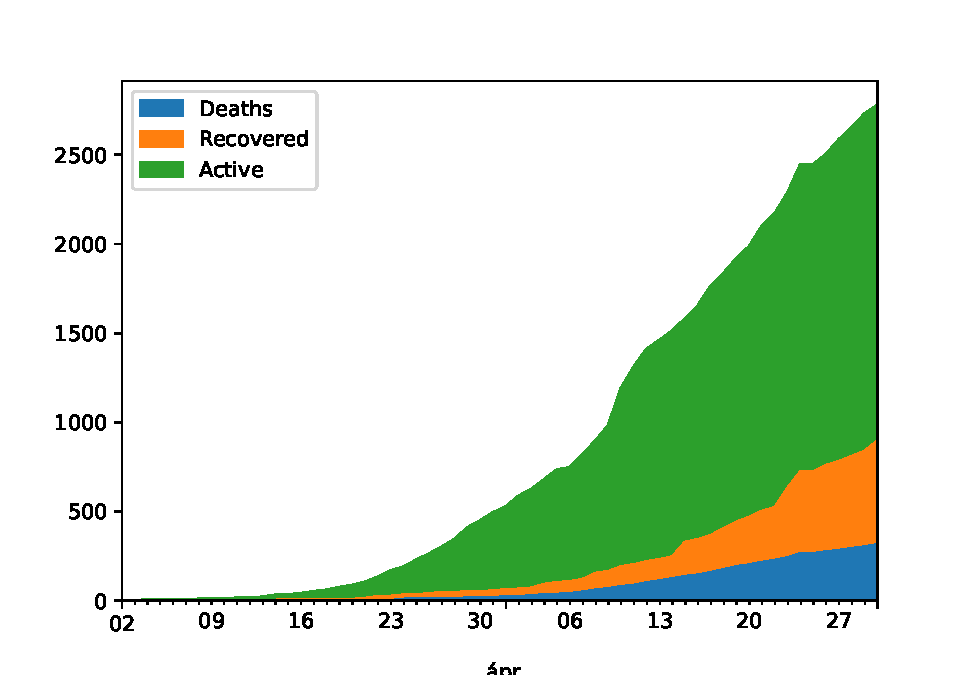
\includegraphics{_main_files/figure-latex/unnamed-chunk-87-1.pdf}

\section{Aggregálás data frame-ben}\label{aggreguxe1luxe1s-data-frame-ben}

Szűrjük le a corona dataframe-ből a legfrissebb adatokat minden országra egy új, corona\_latest dataframe-be!
Maximum függvényünk a \texttt{numpy} csomagból, tehát az \texttt{np} névtérből van.

\begin{Shaded}
\begin{Highlighting}[]
\NormalTok{corona\_latest }\OperatorTok{=}\NormalTok{ corona[corona[}\StringTok{\textquotesingle{}Date\textquotesingle{}}\NormalTok{]}\OperatorTok{==}\NormalTok{np.}\BuiltInTok{max}\NormalTok{(corona[}\StringTok{\textquotesingle{}Date\textquotesingle{}}\NormalTok{])]}
\NormalTok{corona\_latest.info()}
\end{Highlighting}
\end{Shaded}

\begin{verbatim}
## <class 'pandas.core.frame.DataFrame'>
## Index: 264 entries, 26136 to 26399
## Data columns (total 9 columns):
##  #   Column          Non-Null Count  Dtype         
## ---  ------          --------------  -----         
##  0   Province/State  264 non-null    object        
##  1   Country/Region  264 non-null    object        
##  2   Lat             264 non-null    float64       
##  3   Long            264 non-null    float64       
##  4   Date            264 non-null    datetime64[ns]
##  5   Confirmed       264 non-null    int64         
##  6   Deaths          264 non-null    int64         
##  7   Recovered       264 non-null    int64         
##  8   Active          264 non-null    int64         
## dtypes: datetime64[ns](1), float64(2), int64(4), object(2)
## memory usage: 20.6+ KB
\end{verbatim}

Itt mivel egy ország akár lehet több régióval is jelen a sorok között országnév szerint össze tudjuk adni az összes megerősített koronavírusos esetet (\emph{Confirmed} oszlop elemei). Magyarul \textbf{ország szintre szeretnénk összeg segítségével aggregálni} a megerősített koronavírus esetek számát.

Ehhez először a data frame \texttt{groupby} metódusával csoportosítani kell a sorokat ország szintre, majd megadni az összegzendő oszlopot és elsütni ezen oszlop \texttt{sum} metódusát az összegzéshez. Ha a \texttt{sum}-ot \texttt{avg}-re vagy \texttt{median}-ra cseréljük, akkor a kiválasztott oszlopnak nem az összegét, hanem az átlagát, illetve mediánját tudjuk nézni országok szerint. Azaz \textbf{átlaggal/mediánnal is aggregálhatunk az országok szintjére}.

\begin{Shaded}
\begin{Highlighting}[]
\NormalTok{corona\_country }\OperatorTok{=}\NormalTok{ corona\_latest.groupby(}\StringTok{\textquotesingle{}Country/Region\textquotesingle{}}\NormalTok{)[}\StringTok{\textquotesingle{}Confirmed\textquotesingle{}}\NormalTok{].}\BuiltInTok{sum}\NormalTok{()}

\NormalTok{corona\_country.info()}
\end{Highlighting}
\end{Shaded}

\begin{verbatim}
## <class 'pandas.core.series.Series'>
## Index: 187 entries, Afghanistan to Zimbabwe
## Series name: Confirmed
## Non-Null Count  Dtype
## --------------  -----
## 187 non-null    int64
## dtypes: int64(1)
## memory usage: 2.9+ KB
\end{verbatim}

\begin{Shaded}
\begin{Highlighting}[]
\NormalTok{corona\_country.head()}
\end{Highlighting}
\end{Shaded}

\begin{verbatim}
## Country/Region
## Afghanistan    2171
## Albania         773
## Algeria        4006
## Andorra         745
## Angola           27
## Name: Confirmed, dtype: int64
\end{verbatim}

Az eredmény nem egy data frame, hanem mint láthatjuk egy \texttt{Series} lett, ami ugyebár logikailag egy \texttt{numpy} tömb! Mivel a \texttt{groupby} során az országok nevéből lett az új sorindex, így csak 1 oszlopunk maradt, az összegzett megerősített esetszám.

Ha azt szeretnénk, hogy a \textbf{corona\_country}-ben az országok neve ne indexként, hanem külön oszlopként szerepeljen, akkor használjuk a \texttt{reset\_index()} metódust!

\begin{Shaded}
\begin{Highlighting}[]
\NormalTok{corona\_country }\OperatorTok{=}\NormalTok{ corona\_country.reset\_index()}

\NormalTok{corona\_country.info()}
\end{Highlighting}
\end{Shaded}

\begin{verbatim}
## <class 'pandas.core.frame.DataFrame'>
## RangeIndex: 187 entries, 0 to 186
## Data columns (total 2 columns):
##  #   Column          Non-Null Count  Dtype 
## ---  ------          --------------  ----- 
##  0   Country/Region  187 non-null    object
##  1   Confirmed       187 non-null    int64 
## dtypes: int64(1), object(1)
## memory usage: 3.1+ KB
\end{verbatim}

\begin{Shaded}
\begin{Highlighting}[]
\NormalTok{corona\_country.head()}
\end{Highlighting}
\end{Shaded}

\begin{verbatim}
##   Country/Region  Confirmed
## 0    Afghanistan       2171
## 1        Albania        773
## 2        Algeria       4006
## 3        Andorra        745
## 4         Angola         27
\end{verbatim}

Amennyiben a \texttt{groupby} metódus után egy általánosabb \texttt{agg} metódust használunk, akkor a \texttt{groupby}-ban megadott csoportosítás szerint egyszerre több művelet segítségével is összesíthetjük, azaz aggregálhatjuk a számértékű oszlop értékeit (pl. egyszerre nézünk átlagos és medián esetszámokat), Vagy akár több számértékű oszlopot is aggregálhatunk a \texttt{groupby} paraméterei szerint (pl. egyszerre nézünk átlagos esetszámot és halálozást is). Ráadásul, el is tudjuk nevezni az \texttt{agg} függvényen belül az újonnan létrehozott összesítő, azaz aggregált oszlopokat!
Annyi trükk van a dologban, hogy az aggregáláshoz használt függvényeket (medián, átlag, szórás, stb.) a \texttt{numpy} csomagból szedjük ki az \texttt{np.} előtaggal!

Szóval a következő kódrészletben az \texttt{AtlagAktiv\ =\ ("Active",\ np.mean)} rész azt jelenti majd pl, hogy az \emph{AtlagAktiv} oszlop a létrehozandó kimutatástáblában az eredeti data frame \emph{Active} oszlopának átlaggal, azaz \texttt{np.mean} függvényével országos szintre összesített (``\emph{groupby}''-olt) értékeit tartalmazza.

Na, akkor mostmár tényleg készítsünk el egy ország szintű kimutatást az átlagos és medián aktív koronavírus eseteiről, illetve átlagos és medián halálozási számairól a legfrisebb dátumra! Azt is megtehetjük, hogy már az aggregáló kód végére rögtön odatoljuk a \texttt{reset\_index}-et.

\begin{Shaded}
\begin{Highlighting}[]
\NormalTok{corona\_kimutatas }\OperatorTok{=}\NormalTok{ corona\_latest.groupby(}\StringTok{\textquotesingle{}Country/Region\textquotesingle{}}\NormalTok{).agg(}
\NormalTok{  AtlagAktiv }\OperatorTok{=}\NormalTok{ (}\StringTok{"Active"}\NormalTok{, np.mean),}
\NormalTok{  MedianAktiv }\OperatorTok{=}\NormalTok{ (}\StringTok{"Active"}\NormalTok{, np.median),}
\NormalTok{  AtlagHalal }\OperatorTok{=}\NormalTok{ (}\StringTok{"Deaths"}\NormalTok{, np.mean),}
\NormalTok{  MedianHalal }\OperatorTok{=}\NormalTok{ (}\StringTok{"Deaths"}\NormalTok{, np.median)}
\NormalTok{).reset\_index()}
\end{Highlighting}
\end{Shaded}

\begin{verbatim}
## <string>:1: FutureWarning: The provided callable <function mean at 0x000001CA046C13A0> is currently using SeriesGroupBy.mean. In a future version of pandas, the provided callable will be used directly. To keep current behavior pass the string "mean" instead.
## <string>:1: FutureWarning: The provided callable <function median at 0x000001CA04888720> is currently using SeriesGroupBy.median. In a future version of pandas, the provided callable will be used directly. To keep current behavior pass the string "median" instead.
## <string>:1: FutureWarning: The provided callable <function mean at 0x000001CA046C13A0> is currently using SeriesGroupBy.mean. In a future version of pandas, the provided callable will be used directly. To keep current behavior pass the string "mean" instead.
\end{verbatim}

\begin{Shaded}
\begin{Highlighting}[]
\NormalTok{corona\_kimutatas}
\end{Highlighting}
\end{Shaded}

\begin{verbatim}
##          Country/Region  AtlagAktiv  MedianAktiv  AtlagHalal  MedianHalal
## 0           Afghanistan      1847.0       1847.0        64.0         64.0
## 1               Albania       272.0        272.0        31.0         31.0
## 2               Algeria      1777.0       1777.0       450.0        450.0
## 3               Andorra       235.0        235.0        42.0         42.0
## 4                Angola        18.0         18.0         2.0          2.0
## ..                  ...         ...          ...         ...          ...
## 182  West Bank and Gaza       266.0        266.0         2.0          2.0
## 183      Western Sahara         1.0          1.0         0.0          0.0
## 184               Yemen         4.0          4.0         2.0          2.0
## 185              Zambia        48.0         48.0         3.0          3.0
## 186            Zimbabwe        31.0         31.0         4.0          4.0
## 
## [187 rows x 5 columns]
\end{verbatim}

Azt látjuk, hogy az átlag és medián értékek mind az aktív esetek számára, mind a halálozási számokra megegyeznek. Ez azért van, mert a legtöbb ország ugyebár nem volt lebontva államokra és provinciákra, szóval egy nap csak egy érték érkezett a táblába rájuk mindenből. Egy értéknek pedig nyilván ugyan az az átlaga és a mediánja is! :)

Na, de lessünk meg pár olyan országot, ahol az adatok belső régiókra, provinciákra is le voltak bontva. Pl. Franciaország és az Egyesült Királyság ilyen országok voltak:

\begin{Shaded}
\begin{Highlighting}[]
\NormalTok{corona\_kimutatas[corona\_kimutatas[}\StringTok{"Country/Region"}\NormalTok{].isin([}\StringTok{"France"}\NormalTok{, }\StringTok{"United Kingdom"}\NormalTok{])]}
\end{Highlighting}
\end{Shaded}

\begin{verbatim}
##      Country/Region    AtlagAktiv  MedianAktiv   AtlagHalal  MedianHalal
## 62           France   8409.909091         31.0  2219.090909          1.0
## 177  United Kingdom  13161.818182         13.0  2440.181818          1.0
\end{verbatim}

Na itt már látszik az eltérés! Pl. a francia tartományok felében legfeljebb \(31\) aktív koronavírusos eset volt csak 2020.04.30-án, de a tartományok átlagában az érték már kerektíve \(8410\) eset! Ezt valószínűleg egy vagy kettő kiugróan sok esettel rendlkező tartomány okozza csak!

\section{Egyszerű leíró statisztika data frame-ben}\label{egyszerux171-leuxedruxf3-statisztika-data-frame-ben}

No, de most térjünk vissza a \textbf{corona\_country} data frame-hez! Egyszerűsítsük az oszlopneveket! A data frame-k \texttt{columns} tulajdonságának felülírásával az oszlopnevek könnyen módosíthatók. Mivel ugye a \texttt{columns} tulajdonságban az összes oszlopnév szerepel listaként, így az új oszlopneveket listaként felsorolva {[}{]} jellel kell megadni.

\begin{Shaded}
\begin{Highlighting}[]
\NormalTok{corona\_country.columns}\OperatorTok{=}\NormalTok{[}\StringTok{\textquotesingle{}Country\textquotesingle{}}\NormalTok{, }\StringTok{\textquotesingle{}COVID\_Cases\textquotesingle{}}\NormalTok{]}

\NormalTok{corona\_country.info()}
\end{Highlighting}
\end{Shaded}

\begin{verbatim}
## <class 'pandas.core.frame.DataFrame'>
## RangeIndex: 187 entries, 0 to 186
## Data columns (total 2 columns):
##  #   Column       Non-Null Count  Dtype 
## ---  ------       --------------  ----- 
##  0   Country      187 non-null    object
##  1   COVID_Cases  187 non-null    int64 
## dtypes: int64(1), object(1)
## memory usage: 3.1+ KB
\end{verbatim}

Nézzünk egy komplett leíró statisztikát a \emph{COVID\_Cases} változóra/ismérvre/oszlopra a \texttt{describe} metódus segítségével. Kerekítsük az eredményeket 2 tizedesjegyre (\texttt{round} függvény).

\begin{Shaded}
\begin{Highlighting}[]
\BuiltInTok{round}\NormalTok{(corona\_country.COVID\_Cases.describe(),}\DecValTok{2}\NormalTok{)}
\end{Highlighting}
\end{Shaded}

\begin{verbatim}
## count        187.00
## mean       17416.26
## std        84414.11
## min            1.00
## 25%           97.50
## 50%          746.00
## 75%         6254.50
## max      1069424.00
## Name: COVID_Cases, dtype: float64
\end{verbatim}

Nézzük meg ezt az ordenáré módon jobbra elnyúló eloszlást hisztogramon és doboz ábrán is!

A hisztogramot simán a vizsgált oszlop \texttt{hist} metódusával le lehet kérni.

\begin{Shaded}
\begin{Highlighting}[]
\NormalTok{corona\_country.COVID\_Cases.hist()}
\end{Highlighting}
\end{Shaded}

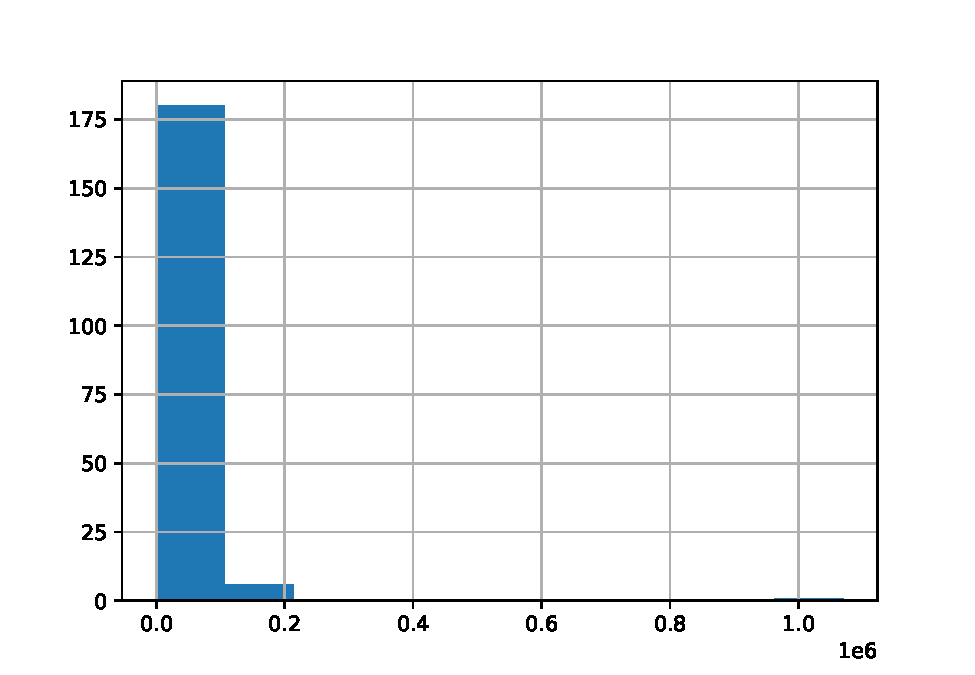
\includegraphics{_main_files/figure-latex/unnamed-chunk-95-3.pdf}

Alapból egyenlő hosszúságú osztályközötket képez a pitonállat a hisztogramokhoz, aminek a számát a \texttt{hist} függvényben a \texttt{bins} paraméteren keresztül tudjuk szabályozni.

Vigyük le pl. az osztályközök számát \(5\)-re.

\begin{Shaded}
\begin{Highlighting}[]
\NormalTok{corona\_country.COVID\_Cases.hist(bins}\OperatorTok{=}\DecValTok{5}\NormalTok{)}
\end{Highlighting}
\end{Shaded}

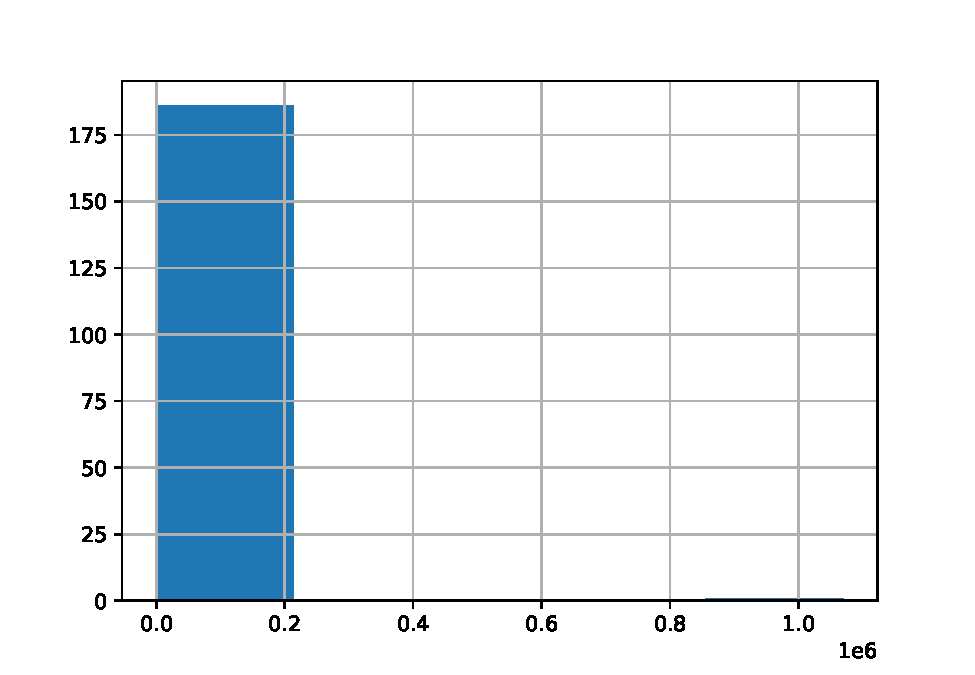
\includegraphics{_main_files/figure-latex/unnamed-chunk-96-5.pdf}

A \texttt{boxplot} metódus már alapvetően data frame, és nem oszlop szinten működik, és a metódus paraméterében kell megadni, hogy mely oszlopra vagy oszlopokra (neveket listaként felsorolva {[}{]} jellel) akarjuk az ábrát. Tehát, a doboz ábrát egyszerre több oszlopra is lekérhetjük egy ábrán belülre akár. Majd mindjárt nézünk ilyet is. Ennek a doboz ábránál van értelme, hiszen doboz ábránál nincsenek osztályközök, amiknek a számát esetlegesen az ismérvünk (oszlopunk) eloszlására kell szabni.

\begin{Shaded}
\begin{Highlighting}[]
\NormalTok{corona\_country.boxplot(column}\OperatorTok{=}\StringTok{"COVID\_Cases"}\NormalTok{)}
\end{Highlighting}
\end{Shaded}

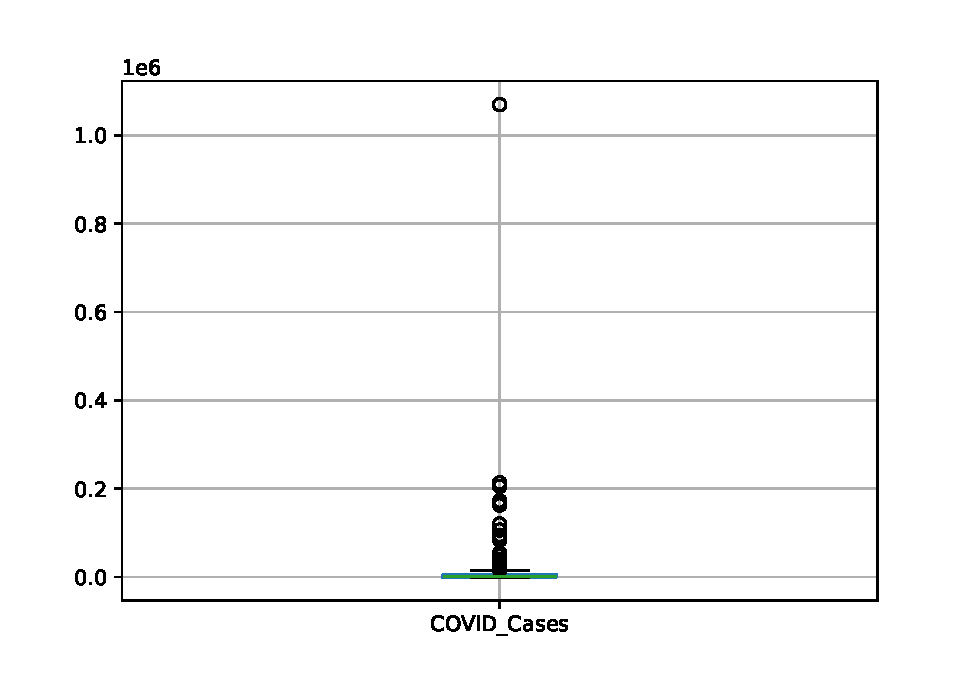
\includegraphics{_main_files/figure-latex/unnamed-chunk-97-7.pdf}

\section{Adatminőségi problémák felismerése és kezelése leíró statisztika segítségével}\label{adatminux151suxe9gi-probluxe9muxe1k-felismeruxe9se-uxe9s-kezeluxe9se-leuxedruxf3-statisztika-seguxedtsuxe9guxe9vel}

Olvassuk be a population\_by\_country\_2020.csv nevű fájlt, és mentsük el a beolvasott adatokat egy \textbf{population} nevű data frame-be!

\begin{Shaded}
\begin{Highlighting}[]
\NormalTok{population }\OperatorTok{=}\NormalTok{ pd.read\_csv(}\StringTok{\textquotesingle{}population\_by\_country\_2020.csv\textquotesingle{}}\NormalTok{)}
\NormalTok{population.info()}
\end{Highlighting}
\end{Shaded}

\begin{verbatim}
## <class 'pandas.core.frame.DataFrame'>
## RangeIndex: 235 entries, 0 to 234
## Data columns (total 11 columns):
##  #   Column                   Non-Null Count  Dtype  
## ---  ------                   --------------  -----  
##  0   Country (or dependency)  235 non-null    object 
##  1   Population (2020)        235 non-null    int64  
##  2   Yearly Change            235 non-null    object 
##  3   Net Change               235 non-null    int64  
##  4   Density (P/Km²)          235 non-null    int64  
##  5   Land Area (Km²)          235 non-null    int64  
##  6   Migrants (net)           201 non-null    float64
##  7   Fert. Rate               235 non-null    object 
##  8   Med. Age                 235 non-null    object 
##  9   Urban Pop %              235 non-null    object 
##  10  World Share              235 non-null    object 
## dtypes: float64(1), int64(4), object(6)
## memory usage: 20.3+ KB
\end{verbatim}

A \textbf{population} dataframe-ből csak az országnév, népesség, népsűrűség és városi népesség aránya változókra lesz szükségünk.
A többit törölhetjük is a data frame-ből! Mivel az oszlopnevekben mint fentebb láthatjuk elég sok a hányadék módon speciális karakter, így biztonságosabb most az oszlopokra a sorszámukkal hivatkozni. Láthatjuk az \texttt{info} metódus eredményéből, hogy a szükséges országnév, népesség, népsűrűség és városi népesség aránya oszlopok rendre a \(0,1,4,9\) indexekkel bírnak.

\begin{Shaded}
\begin{Highlighting}[]
\NormalTok{population }\OperatorTok{=}\NormalTok{ population.iloc[:,[}\DecValTok{0}\NormalTok{, }\DecValTok{1}\NormalTok{, }\DecValTok{4}\NormalTok{, }\DecValTok{9}\NormalTok{]]}

\NormalTok{population.info()}
\end{Highlighting}
\end{Shaded}

\begin{verbatim}
## <class 'pandas.core.frame.DataFrame'>
## RangeIndex: 235 entries, 0 to 234
## Data columns (total 4 columns):
##  #   Column                   Non-Null Count  Dtype 
## ---  ------                   --------------  ----- 
##  0   Country (or dependency)  235 non-null    object
##  1   Population (2020)        235 non-null    int64 
##  2   Density (P/Km²)          235 non-null    int64 
##  3   Urban Pop %              235 non-null    object
## dtypes: int64(2), object(2)
## memory usage: 7.5+ KB
\end{verbatim}

Egyszerűsítsük az oszlopneveket a population dataframe-ben!

\begin{Shaded}
\begin{Highlighting}[]
\NormalTok{population.columns }\OperatorTok{=}\NormalTok{ [}\StringTok{\textquotesingle{}Country\textquotesingle{}}\NormalTok{, }\StringTok{\textquotesingle{}Pop\textquotesingle{}}\NormalTok{, }\StringTok{\textquotesingle{}PopDensity\textquotesingle{}}\NormalTok{, }\StringTok{\textquotesingle{}UrbanPop\textquotesingle{}}\NormalTok{]}

\NormalTok{population.info()}
\end{Highlighting}
\end{Shaded}

\begin{verbatim}
## <class 'pandas.core.frame.DataFrame'>
## RangeIndex: 235 entries, 0 to 234
## Data columns (total 4 columns):
##  #   Column      Non-Null Count  Dtype 
## ---  ------      --------------  ----- 
##  0   Country     235 non-null    object
##  1   Pop         235 non-null    int64 
##  2   PopDensity  235 non-null    int64 
##  3   UrbanPop    235 non-null    object
## dtypes: int64(2), object(2)
## memory usage: 7.5+ KB
\end{verbatim}

Nézzük meg a population dataframe egyszerű leíró statisztikai mutatóit! Ha a \texttt{describe} metódust az egész data frame-n engedjük el, akkor minden numerikus (\texttt{int} vagy \texttt{float}) oszlopra megadja az alap leíró mutatókat.

\begin{Shaded}
\begin{Highlighting}[]
\BuiltInTok{round}\NormalTok{(population.describe(), }\DecValTok{2}\NormalTok{)}
\end{Highlighting}
\end{Shaded}

\begin{verbatim}
##                 Pop  PopDensity
## count  2.350000e+02      235.00
## mean   3.316936e+07      475.77
## std    1.351374e+08     2331.29
## min    8.010000e+02        0.00
## 25%    3.988760e+05       37.00
## 50%    5.459642e+06       95.00
## 75%    2.057705e+07      239.50
## max    1.439324e+09    26337.00
\end{verbatim}

Az \emph{UrbanPop} változónak mi baja? Elviekben az egy arányszám, annak is számnak kéne lennie, és meg kéne jelennie a \texttt{describe} metódus eredményében!

Kukkantsunk csak bele a data frame első 5 sorába!

\begin{Shaded}
\begin{Highlighting}[]
\NormalTok{population.head()}
\end{Highlighting}
\end{Shaded}

\begin{verbatim}
##          Country         Pop  PopDensity UrbanPop
## 0          China  1439323776         153      61%
## 1          India  1380004385         464      35%
## 2  United States   331002651          36      83%
## 3      Indonesia   273523615         151      56%
## 4       Pakistan   220892340         287      35%
\end{verbatim}

Áhhá! Százalékjel van benne! Ezért veszi szöveges adatnak a pitonállat!

Szedjük le ezt a százalékjelet! Erre szerencsére az egyes data frame oszlopoknak van egy \texttt{str.replace} metódusa, amiben megadhatjuk paraméterekkel, hogy az oszlopban milyen szövegrészleteket mire akarunk cserélni. Itt most ugyebár százalékjelet fogunk üres stringre cserélni.

\begin{Shaded}
\begin{Highlighting}[]
\NormalTok{population[}\StringTok{\textquotesingle{}UrbanPop\textquotesingle{}}\NormalTok{] }\OperatorTok{=}\NormalTok{ population[}\StringTok{\textquotesingle{}UrbanPop\textquotesingle{}}\NormalTok{].}\BuiltInTok{str}\NormalTok{.replace(}\StringTok{\textquotesingle{}\%\textquotesingle{}}\NormalTok{, }\StringTok{\textquotesingle{}\textquotesingle{}}\NormalTok{)}

\NormalTok{population.head()}
\end{Highlighting}
\end{Shaded}

\begin{verbatim}
##          Country         Pop  PopDensity UrbanPop
## 0          China  1439323776         153       61
## 1          India  1380004385         464       35
## 2  United States   331002651          36       83
## 3      Indonesia   273523615         151       56
## 4       Pakistan   220892340         287       35
\end{verbatim}

Ez jó, de sajnos vannak benne hiányzó értékek, amik nem a szabványos Python \texttt{NaN} kóddal vannak jelölve, hanem ilyen spéci \emph{``N.A.''} stringgel, amit a gépállat nem ismer fel, így az egész oszlopot \texttt{str}-nek (\texttt{object}) veszi a \texttt{numpy} tömbök egységes adattípus logikája alapján.

\begin{Shaded}
\begin{Highlighting}[]
\NormalTok{population.info()}
\end{Highlighting}
\end{Shaded}

\begin{verbatim}
## <class 'pandas.core.frame.DataFrame'>
## RangeIndex: 235 entries, 0 to 234
## Data columns (total 4 columns):
##  #   Column      Non-Null Count  Dtype 
## ---  ------      --------------  ----- 
##  0   Country     235 non-null    object
##  1   Pop         235 non-null    int64 
##  2   PopDensity  235 non-null    int64 
##  3   UrbanPop    235 non-null    object
## dtypes: int64(2), object(2)
## memory usage: 7.5+ KB
\end{verbatim}

Azt, hogy az \texttt{object} adattípus turpisságát az ``N.A.''-k okozzák az UrbanPop oszlopban, arra leginkább az oszlop gyakorisági táblájából lehet felismerni. Ezt a gyakorisági táblát az oszlop \texttt{value\_counts} metódusával tudjuk lekérni.

\begin{Shaded}
\begin{Highlighting}[]
\NormalTok{population.UrbanPop.value\_counts()}
\end{Highlighting}
\end{Shaded}

\begin{verbatim}
## UrbanPop
## N.A.    13
## 57       7
## 88       7
## 63       6
## 87       6
##         ..
## 50       1
## 81       1
## 28       1
## 37       1
## 10       1
## Name: count, Length: 81, dtype: int64
\end{verbatim}

Láthatjuk, hogy a sok számérték mellett, 13 ország esetén hiányzó értékünk van ezzel a csúnya ``N.A.'' kóddal.

Na, akkor! Most csináljuk azt, hogy leszűrjük azt a 13 országot, ahol hiányzik a városi népesség arányára vonatkozó adat!

Ezek után próbáljuk meg a városi népesség arányára vonatkozó adatot \texttt{int} típusúvá konvertálni! Ha sikerült, nézzük meg a változó alap leíró statisztikai mutatóit is!

Először logikai indexszeléssel leszűrjük az ``N.A.''-kat.

\begin{Shaded}
\begin{Highlighting}[]
\NormalTok{population }\OperatorTok{=}\NormalTok{ population[population[}\StringTok{\textquotesingle{}UrbanPop\textquotesingle{}}\NormalTok{]}\OperatorTok{!=}\StringTok{"N.A."}\NormalTok{]}
\end{Highlighting}
\end{Shaded}

Majd az oszlop \texttt{astype} metódusával \texttt{int}-é konvertáljuk az egész oszlopot. A metódus paraméterében kell megadni, hogy milyen adattípusra akarjuk konvertálni kiszemelt kis oszlopunk! :) Végül jöhet a \texttt{describe}.

\begin{Shaded}
\begin{Highlighting}[]
\NormalTok{population[}\StringTok{\textquotesingle{}UrbanPop\textquotesingle{}}\NormalTok{] }\OperatorTok{=}\NormalTok{ population[}\StringTok{\textquotesingle{}UrbanPop\textquotesingle{}}\NormalTok{].astype(}\BuiltInTok{int}\NormalTok{)}

\NormalTok{population.describe()}
\end{Highlighting}
\end{Shaded}

\begin{verbatim}
##                 Pop   PopDensity    UrbanPop
## count  2.220000e+02   222.000000  222.000000
## mean   3.488611e+07   186.373874   59.234234
## std    1.388508e+08   288.271695   24.230400
## min    1.357000e+03     0.000000    0.000000
## 25%    5.444048e+05    35.000000   43.000000
## 50%    5.911701e+06    89.000000   60.500000
## 75%    2.321589e+07   224.500000   79.000000
## max    1.439324e+09  2239.000000  100.000000
\end{verbatim}

Úgy tűnik, helyreállt a világ rendje! Már nagyon szépen le tudjuk olvasni pl., hogy a Föld országainak legzsúfoltabb \(25\%\)-ban legalább \(79\) fő/Km² a népsűrűség. És azt is látni a \texttt{count}ból, hogy már csak \(222\) országunk van a kezdeti \(235\) helyett, szóval nincsen itt a \(13\) ``N.A.''.

\section{Data frame-k összekapcsolása}\label{data-frame-k-uxf6sszekapcsoluxe1sa}

Akkor most álmodjunk egy nagyot! Kössük össze a \textbf{population} data frame-ben található országonkénti alapvető demográfiai ismérveket a \textbf{corona\_country} data frame-ben lakó országonkénti koronavírus esetszámokkal.

Nyilván ezt az összekötést az országok nevén keresztül lehet megtenni. Azaz pl. a magyar koronavírus esetszámokhoz a magyar demográfiai adatoknak kell kerülnie értelemszerűen. :)

A \texttt{pandas} csomagnak létezik egy \texttt{merge} névre hallgató függvénye, ami két data frame-et összeköt egy előre megadott közös oszlop alapján. Esetünkben ez a közös oszlop az országnév lesz.
Ha egy kicsit ``\emph{adatbázisabbul}'' szeretném kifejezni magam, akkor azt mondanám, hogy a \texttt{merge} függvény 2 tábla joinját oldja meg egy közös kulcs alapján.

Sőt, a \texttt{merge} függvény mindhárom alapvető táblakapcsolási módszert támogatja:

\begin{itemize}
\tightlist
\item
  \textbf{inner join}: Az összekötött táblában csak azok a sorok maradnak meg, amelyek mindkét data frame-ben szerepelnek.
\item
  \textbf{left join}: Az összekötött táblában csak azok a sorok maradnak meg, amelyek az elsőre megnevezett data frame-ben szerepelnek (attól függetlenül, hogy a másodszorra megnevezett táblában van-e hozzájuk találat).
\item
  \textbf{right join}: Az összekötött táblában csak azok a sorok maradnak meg, amelyek a másodszorra megnevezett data frame-ben szerepelnek (attól függetlenül, hogy az elsőre megnevezett táblában van-e hozzájuk találat).
\item
  \textbf{full outer join}: Az összekötött táblában mindkét tábla minden sora megmarad.
\end{itemize}

A különböző típusú összekötési módokat remekül lehet halmazábrákkal szemléltetni:

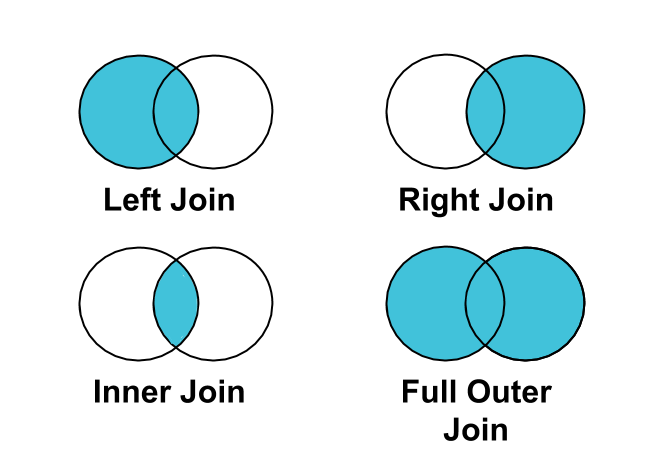
\includegraphics[width=0.5\textwidth,height=\textheight]{JoinVennDiagram.png}

Na, akkor mielőtt a tényleges \texttt{merge}-hez hozzálátunk, annyit ellenőrizzünk le, hogy ugyanaz-e a neve az országneveket tartalmazó oszlopnak mindkét data frame-ben, a \textbf{population}ben és a \textbf{corona\_country}-ban is:

\begin{Shaded}
\begin{Highlighting}[]
\NormalTok{corona\_country.columns}
\end{Highlighting}
\end{Shaded}

\begin{verbatim}
## Index(['Country', 'COVID_Cases'], dtype='object')
\end{verbatim}

\begin{Shaded}
\begin{Highlighting}[]
\NormalTok{population.columns}
\end{Highlighting}
\end{Shaded}

\begin{verbatim}
## Index(['Country', 'Pop', 'PopDensity', 'UrbanPop'], dtype='object')
\end{verbatim}

Szuper, mindkét táblában egységesen \textbf{`Country'} az összekötésre használandó oszlop neve! Nem meglepő, mert mindkét táblában átneveztük már korábban az oszlopokat, de azért jobb biztosra menni. :)

Akkor lássuk azt a \texttt{merge}-t! Most egy olyan összekötést csinálunk, hogy a \textbf{corona\_country} táblában lévő összes sorunk maradjon meg az összekötött táblában, mert alapvetően azok az országok érdekelnek, ahol megvan a COVID fertőzöttek száma. Ez az én data frame megadási sorrendben majd egy \emph{left join}t fog jelenteni. :)

A \texttt{merge} függvényben a két data frame megadása után a \texttt{how} paraméter szabályozza a \emph{join} jellegét, míg az \texttt{on} paraméterben adjuk meg az összekötésre használt oszlop nevét. A \emph{join} tehát azért lesz \emph{left}, mert a \textbf{corona\_country}-t adtam meg először, azaz ``\emph{balrább}''. :)

\begin{Shaded}
\begin{Highlighting}[]
\NormalTok{corona\_extended }\OperatorTok{=}\NormalTok{ pd.merge(corona\_country, population, how}\OperatorTok{=}\StringTok{\textquotesingle{}left\textquotesingle{}}\NormalTok{, on}\OperatorTok{=}\StringTok{\textquotesingle{}Country\textquotesingle{}}\NormalTok{)}
\NormalTok{corona\_extended.info()}
\end{Highlighting}
\end{Shaded}

\begin{verbatim}
## <class 'pandas.core.frame.DataFrame'>
## RangeIndex: 187 entries, 0 to 186
## Data columns (total 5 columns):
##  #   Column       Non-Null Count  Dtype  
## ---  ------       --------------  -----  
##  0   Country      187 non-null    object 
##  1   COVID_Cases  187 non-null    int64  
##  2   Pop          168 non-null    float64
##  3   PopDensity   168 non-null    float64
##  4   UrbanPop     168 non-null    float64
## dtypes: float64(3), int64(1), object(1)
## memory usage: 7.4+ KB
\end{verbatim}

Na, hát az új data frame \texttt{info} metódusa alapján van egy kis probléma. \(187-168=19\) országra a \textbf{corona\_country} data frame-ben nem volt találat a \textbf{population} data frame-ben.

\subsection{A kapcsolási kulcsnak használt oszlop ellenőrzése és javítása}\label{a-kapcsoluxe1si-kulcsnak-hasznuxe1lt-oszlop-ellenux151rzuxe9se-uxe9s-javuxedtuxe1sa}

Lessük meg mik ezek az országok, ahol nem volt találat a \textbf{population} data frame-ben! Ezt pl. úgy tudjuk megtenni, hogy lekérdezzük a hiányzó értékek országát a \textbf{Pop} oszlopban.

\begin{Shaded}
\begin{Highlighting}[]
\NormalTok{corona\_extended.Country[corona\_extended.Pop.isnull()}\OperatorTok{==}\VariableTok{True}\NormalTok{]}
\end{Highlighting}
\end{Shaded}

\begin{verbatim}
## 27                                Burma
## 39                  Congo (Brazzaville)
## 40                     Congo (Kinshasa)
## 42                        Cote d'Ivoire
## 46                              Czechia
## 48                     Diamond Princess
## 75                             Holy See
## 91                               Kosovo
## 92                               Kuwait
## 102                          MS Zaandam
## 113                              Monaco
## 140               Saint Kitts and Nevis
## 142    Saint Vincent and the Grenadines
## 144               Sao Tome and Principe
## 150                           Singapore
## 164                             Taiwan*
## 173                                  US
## 180                           Venezuela
## 182                  West Bank and Gaza
## Name: Country, dtype: object
\end{verbatim}

Elnézegetve az országneveket kialakulhat bennünk valami sejtés: valószínűleg ezeket az országokat máshogy hívják a \textbf{population} data frame-ben, mint a \textbf{corona\_country}-ban. Pl. \emph{Taiwan} nevében valószínűleg nem lesz csillag, vagy \emph{Czechia}-t inkább a hivatalosabb nevén jegyezheti a \textbf{population} tábla: \emph{Czech Republic}. Esetleg a \emph{US} is inkább \emph{United States}-ként szerepelhet.

Teszteljük le ezeket az elméleteket egy egyszerű logikai indexes szűréssel az \texttt{isin} metódussal megtámogatva.

\begin{Shaded}
\begin{Highlighting}[]
\NormalTok{population.Country[population.Country.isin([}\StringTok{"Czech Republic"}\NormalTok{, }\StringTok{"Taiwan"}\NormalTok{, }\StringTok{"United States"}\NormalTok{])]}
\end{Highlighting}
\end{Shaded}

\begin{verbatim}
## 2     United States
## 56           Taiwan
## Name: Country, dtype: object
\end{verbatim}

Mintha bejönne az okoskodásunk, de a cseheket csak nem akarja megtalálni a cucc. Próbáljunk meg úgy szűrni, hogy ne pontosan keressük ezeket az országneveket, hanem azt nézzük meg, hogy mik azok a sorok a \textbf{population} data frame-ben, amik ezeket az országneveket \emph{tartalmazzák} valahol a \textbf{Country} oszlopban.
Ezt egyszerűen el tudjuk érni úgy, hogy az előző kódunkban az \texttt{isin} metódust \texttt{str.contains}-re cseréljük. Annyi van, hogy itt a keresett string mintázatokat egy stringben kell megadni (azaz NEM listaként) ``\textbar{}'' jellel elválasztva őket.
Ez így amúgy egy úgynevezett \href{http://vbence.web.elte.hu/regex_leiras.html}{RegEx kifejezés}, és ilyenekkel lehet komplexebben működtetni ezt a \texttt{str.contains} metódust. Az érdeklődőknek jó kiindulópont a link. :)

\begin{Shaded}
\begin{Highlighting}[]
\NormalTok{population.Country[population.Country.}\BuiltInTok{str}\NormalTok{.contains(}\StringTok{"Czech Republic|Taiwan|United States"}\NormalTok{)]}
\end{Highlighting}
\end{Shaded}

\begin{verbatim}
## 2                United States
## 56                      Taiwan
## 85    Czech Republic (Czechia)
## Name: Country, dtype: object
\end{verbatim}

Ó, hogy a kedves felmenőiket a \textbf{population} data frame alkotóinak: hát nem ott van zárójelben a \emph{Czech Republic} mögött, hogy \emph{Czechia}?! ``\emph{Ripsz!}''

Hát valami hasonló módon be kéne lőni a maradék 16 nem egyező országnevet is, de most ezzel nem húzzuk a drága időnket, hanem javítjuk ezt a 3 esetet és újra összekötjük a tábláinkat.
Aki a nem egyértelmű kapcsoló oszlop (kulcs) alapján történő data frame összekötés világában szeretne elmélyedni, neki érdemes lehet majd előbb-utóbb utána néznie a \emph{fuzzy join} technikáknak, amiket a Pythonban pl. a \href{https://stackoverflow.com/questions/13636848/is-it-possible-to-do-fuzzy-match-merge-with-python-pandas}{difflib csomag támogat}. De ezek a megoldások az itteni bevezető példának a kereteit bőven megugorják komplexitásban.

Szóval, akkor a 3 azonosított eltérő országnevet javítsuk a \textbf{population} data frame-ben. Azaz ott átírjuk ezeket az országneveket arra a verzióra, ami a \textbf{corona\_country}-ban is szerepel. Ehhez megint az \texttt{str.replace}-t használjuk, mint anno az \textbf{UrbanPop} oszlop százalékjeleinek eltávolításakor. Ezt mindhárom esetben külön meg kell sajnos tenni.

\begin{Shaded}
\begin{Highlighting}[]
\NormalTok{population[}\StringTok{\textquotesingle{}Country\textquotesingle{}}\NormalTok{] }\OperatorTok{=}\NormalTok{ population[}\StringTok{\textquotesingle{}Country\textquotesingle{}}\NormalTok{].replace(}\StringTok{\textquotesingle{}United States\textquotesingle{}}\NormalTok{, }\StringTok{\textquotesingle{}US\textquotesingle{}}\NormalTok{)}
\NormalTok{population[}\StringTok{\textquotesingle{}Country\textquotesingle{}}\NormalTok{] }\OperatorTok{=}\NormalTok{ population[}\StringTok{\textquotesingle{}Country\textquotesingle{}}\NormalTok{].replace(}\StringTok{\textquotesingle{}Czech Republic (Czechia)\textquotesingle{}}\NormalTok{, }\StringTok{\textquotesingle{}Czechia\textquotesingle{}}\NormalTok{)}
\NormalTok{population[}\StringTok{\textquotesingle{}Country\textquotesingle{}}\NormalTok{] }\OperatorTok{=}\NormalTok{ population[}\StringTok{\textquotesingle{}Country\textquotesingle{}}\NormalTok{].replace(}\StringTok{\textquotesingle{}Taiwan\textquotesingle{}}\NormalTok{, }\StringTok{\textquotesingle{}Taiwan*\textquotesingle{}}\NormalTok{)}
\end{Highlighting}
\end{Shaded}

És akkor lássuk újra azt a \texttt{merge}-t! Most a többi nem kezelt esetet eldobjuk, szóval \emph{inner join}t csinálunk.

\begin{Shaded}
\begin{Highlighting}[]
\NormalTok{corona\_extended }\OperatorTok{=}\NormalTok{ pd.merge(corona\_country, population, how}\OperatorTok{=}\StringTok{\textquotesingle{}inner\textquotesingle{}}\NormalTok{, on}\OperatorTok{=}\StringTok{\textquotesingle{}Country\textquotesingle{}}\NormalTok{)}
\NormalTok{corona\_extended.info()}
\end{Highlighting}
\end{Shaded}

\begin{verbatim}
## <class 'pandas.core.frame.DataFrame'>
## RangeIndex: 171 entries, 0 to 170
## Data columns (total 5 columns):
##  #   Column       Non-Null Count  Dtype 
## ---  ------       --------------  ----- 
##  0   Country      171 non-null    object
##  1   COVID_Cases  171 non-null    int64 
##  2   Pop          171 non-null    int64 
##  3   PopDensity   171 non-null    int64 
##  4   UrbanPop     171 non-null    int32 
## dtypes: int32(1), int64(3), object(1)
## memory usage: 6.1+ KB
\end{verbatim}

Szupszi! Már nem \(168\) sor van, amire van találat mindkét data frame-ben, mint az előbb, hanem \(171\), azaz pont a megjavított \(3\) országgal több! Na, erre már elő lehet venni az ünnepi laposüveget (leánykori nevén lapiüvit)! ;)

\section{Kilógó értékek keresése és kezelése}\label{kiluxf3guxf3-uxe9rtuxe9kek-keresuxe9se-uxe9s-kezeluxe9se}

A sikeres data frame összekötési művelet örömére, számoljuk ki a \textbf{corona\_extended} dataframe-ben az egymillió főre jutó COVID-19 esetek számát minden országra! Aztán nézzük is meg az oszlop leíró statisztikáit!

\begin{Shaded}
\begin{Highlighting}[]
\NormalTok{corona\_extended[}\StringTok{\textquotesingle{}COVID\_perMillion\textquotesingle{}}\NormalTok{] }\OperatorTok{=}\NormalTok{ corona\_extended.COVID\_Cases }\OperatorTok{/}\NormalTok{ corona\_extended.Pop }\OperatorTok{*} \DecValTok{1000000}
\NormalTok{corona\_extended[}\StringTok{\textquotesingle{}COVID\_perMillion\textquotesingle{}}\NormalTok{].describe()}
\end{Highlighting}
\end{Shaded}

\begin{verbatim}
## count      171.000000
## mean       747.439425
## std       1775.534029
## min          0.201167
## 25%         19.420289
## 50%        119.830206
## 75%        700.197689
## max      16769.325985
## Name: COVID_perMillion, dtype: float64
\end{verbatim}

Na, szuper, itt is látszik egy csodás jobbra elnyúló eloszlás, hiszen az országok \(\frac{3}{4}\)-ének az egymillió főre vetített COVID esetszáma nem haladja meg a \(700\)-at, de ellenben a legnagyobb érték már majdnem \(17\) ezer fő! Ellenben az alsó \(25\%\) határa, a \(19.4\) egészen közel van a minimumhoz, a \(0.2\)-höz. Szóval valószínűleg brutál felfelé kilógó elemeink vannak.

Ezt erősítsük is meg egy doboz ábrán.

\begin{Shaded}
\begin{Highlighting}[]
\NormalTok{corona\_extended.boxplot(column}\OperatorTok{=}\StringTok{"COVID\_perMillion"}\NormalTok{)}
\end{Highlighting}
\end{Shaded}

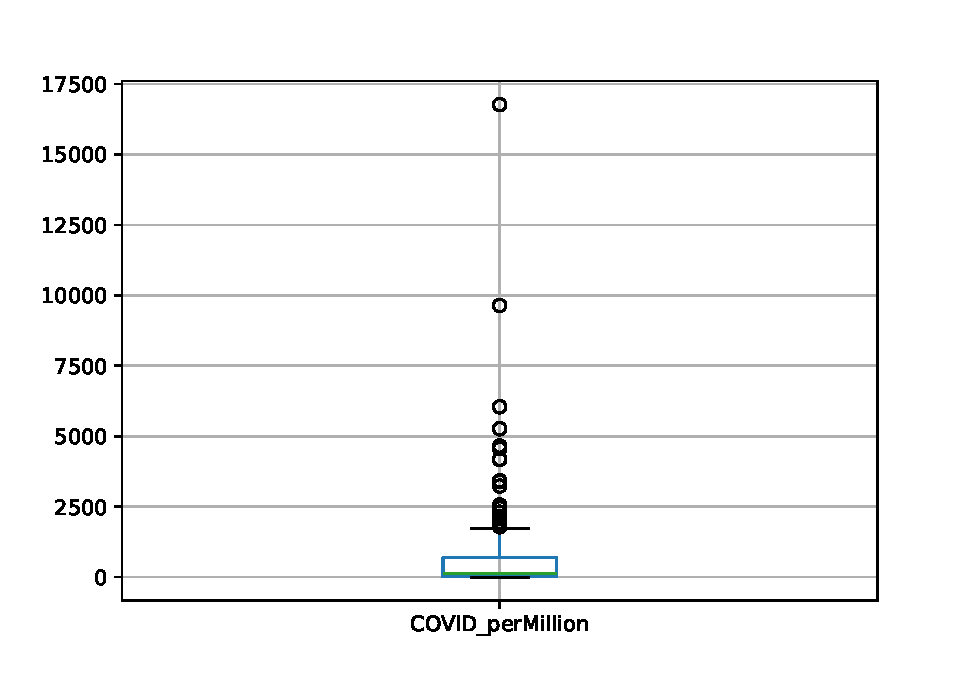
\includegraphics{_main_files/figure-latex/unnamed-chunk-116-9.pdf}

Az ábra alapján nagyjából olyan 3000 feletti értékek tűnnek extrém módon kilógónak (kb. 3000-nél van az első szakadás a dobozban a ponttal jelölt kilógó értékek körében; a szakadás alatti részek, még kb a normál adatok ``természetes'' folytatásának tekinthetők). Lássuk hát, hogy mik ezek!

Rendezzük a \textbf{COVID\_perMillion} szerint csökkenő sorrendbe a data frame-t, és kérjük le a sorbarendezett verzióból azokat az értékeket, ahol a \textbf{COVID\_perMillion} nagyobb, mint 3000!

A data frame-t sorba rendezni a \texttt{sort\_values} metódussal lehet, amelynek paraméterében meg kell adni, hogy mely oszlop alapján rendezünk, és hogy a sorrend csökkenő vagy növekvő-e. Majd ezen a rendezett állapoton elsüthetünk pl. egy iloc-ot az első 10 sor kiválasztásához.

\begin{Shaded}
\begin{Highlighting}[]
\NormalTok{corona\_extended.sort\_values(}\StringTok{\textquotesingle{}COVID\_perMillion\textquotesingle{}}\NormalTok{, ascending}\OperatorTok{=}\VariableTok{False}\NormalTok{).loc[corona\_extended[}\StringTok{\textquotesingle{}COVID\_perMillion\textquotesingle{}}\NormalTok{] }\OperatorTok{\textgreater{}} \DecValTok{3000}\NormalTok{,:]}
\end{Highlighting}
\end{Shaded}

\begin{verbatim}
##          Country  COVID_Cases  ...  UrbanPop  COVID_perMillion
## 131   San Marino          569  ...        97      16769.325985
## 3        Andorra          745  ...        88       9642.140685
## 93    Luxembourg         3784  ...        88       6044.940877
## 72       Iceland         1797  ...        94       5266.042087
## 126        Qatar        13409  ...        96       4654.201086
## 143        Spain       213435  ...        80       4564.987989
## 16       Belgium        48519  ...        98       4186.417453
## 77       Ireland        20612  ...        63       4174.340484
## 148  Switzerland        29586  ...        74       3418.520185
## 79         Italy       205463  ...        69       3398.226842
## 159           US      1069424  ...        83       3230.862341
## 
## [11 rows x 6 columns]
\end{verbatim}

Na, úgy néz ki, hogy az érintett országok töbségében ilyen jó kicsi, zsúfolt államok. Persze vannak extrém kivételek, pl. ugye az olaszok a nagy repülős turistaforgalmuk miatt.

Na, ezeket az extrém módon kilógó értékeket kipucoljuk a data frame-ből, aztán ránézünk újra a \textbf{COVID\_perMillion} doboz ábrájára. Most a kilógó értékeket vegyük csak a 4000 feletti esetszámoknak, mivel a sorrend alapján van egy nagyobb ugrás ott a svájci 3418-ról az ír 4174-re. Meg a doboz ábrán is látszik, hogy ez az utolsó 3 érték ebben a ``toplistában'' még azért közelebb van az adatok ``természetes folytatásához'', és utána jön még egy ugrás az egymillió főre vetített esetszámokban.

\begin{Shaded}
\begin{Highlighting}[]
\NormalTok{corona\_extended }\OperatorTok{=}\NormalTok{ corona\_extended[corona\_extended[}\StringTok{\textquotesingle{}COVID\_perMillion\textquotesingle{}}\NormalTok{] }\OperatorTok{\textless{}} \DecValTok{4000}\NormalTok{]}
\NormalTok{corona\_extended.boxplot(column}\OperatorTok{=}\StringTok{"COVID\_perMillion"}\NormalTok{)}
\end{Highlighting}
\end{Shaded}

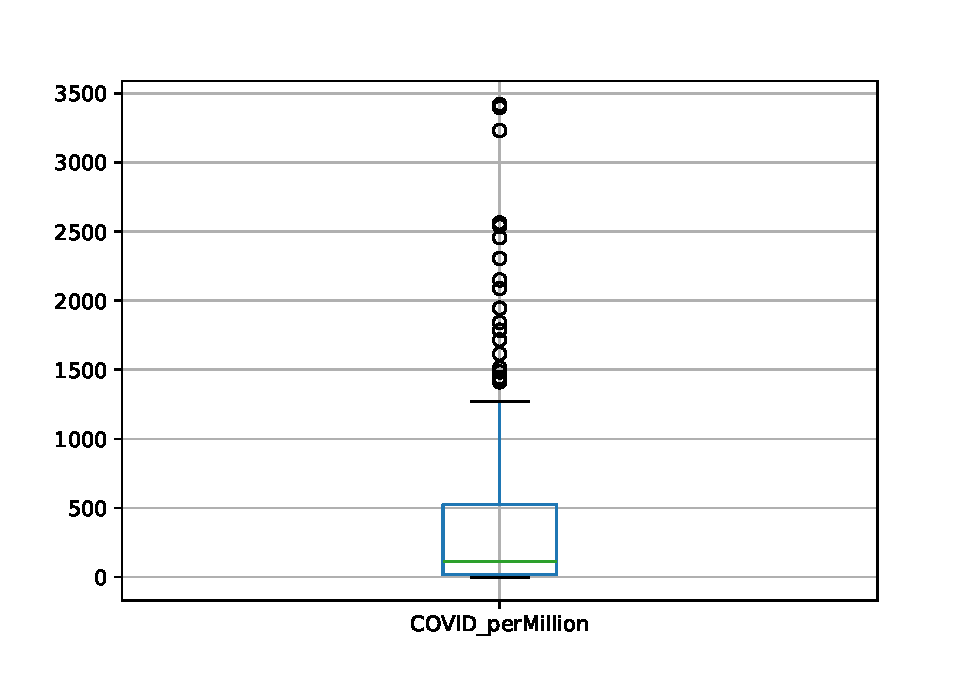
\includegraphics{_main_files/figure-latex/unnamed-chunk-118-11.pdf}

Ez már egy kulturáltabb jobbra elnyúló eloszlás. Viszont, a medián még mindig túlságosan közel van az alsó kvartilishez, és a felső kvartilis eléggé elszakad.

Ennek szellemében még nézzünk rá arra, hogy mely országok esnek az egymillió főre jutó COVID esetszám szerint az alsó kvintilisbe!

Egy data frame oszlop alsó kvintilisét az oszlop \texttt{quantile} metódusával számoljuk ki. A metódus alapvetően egy tetszőleges percentilist számol ki. Azt, hogy melyiket, azt a metódus paraméterében kell megadni \(0-1\) közötti számként. Szóval az alsó kvintilis alias 20. percentilis, ami alatt az adatok \(20\%\)-a található, egy \(0.2\) paraméterrel lesz megadható.

\begin{Shaded}
\begin{Highlighting}[]
\NormalTok{corona\_extended[}\StringTok{\textquotesingle{}COVID\_perMillion\textquotesingle{}}\NormalTok{].quantile(}\FloatTok{0.2}\NormalTok{)}
\end{Highlighting}
\end{Shaded}

\begin{verbatim}
## 10.058723607815136
\end{verbatim}

Ezt a fenti kódot felhasználva egy logikai indexes szűrésben gyorsan meg is lesznek a népességarányos esetszám szerinti alsó kvintilisbe tartozó országok nevei is.

\begin{Shaded}
\begin{Highlighting}[]
\NormalTok{corona\_extended[corona\_extended[}\StringTok{\textquotesingle{}COVID\_perMillion\textquotesingle{}}\NormalTok{] }\OperatorTok{\textless{}} 
\NormalTok{               corona\_extended[}\StringTok{\textquotesingle{}COVID\_perMillion\textquotesingle{}}\NormalTok{].quantile(}\FloatTok{0.2}\NormalTok{)]}
\end{Highlighting}
\end{Shaded}

\begin{verbatim}
##               Country  COVID_Cases  ...  UrbanPop  COVID_perMillion
## 4              Angola           27  ...        67          0.821511
## 18              Benin           64  ...        48          5.279134
## 19             Bhutan            7  ...        46          9.071964
## 22           Botswana           23  ...        73          9.780463
## 27            Burundi           11  ...        14          0.925086
## 29           Cambodia          122  ...        24          7.297102
## 33               Chad           73  ...        23          4.444211
## 37            Comoros            1  ...        29          1.149953
## 54           Ethiopia          131  ...        21          1.139491
## 59             Gambia           11  ...        59          4.551722
## 69              Haiti           81  ...        57          7.103688
## 84              Kenya          396  ...        28          7.364524
## 86               Laos           19  ...        36          2.611483
## 90              Libya           61  ...        78          8.877515
## 94         Madagascar          128  ...        39          4.622437
## 95             Malawi           37  ...        18          1.934140
## 100        Mauritania            8  ...        57          1.720557
## 107        Mozambique           76  ...        38          2.431577
## 108           Namibia           16  ...        55          6.296969
## 109             Nepal           57  ...        21          1.956288
## 112         Nicaragua           14  ...        57          2.113350
## 114           Nigeria         1932  ...        52          9.372290
## 120  Papua New Guinea            8  ...        13          0.894152
## 142       South Sudan           35  ...        25          3.126752
## 149             Syria           43  ...        60          2.457050
## 151        Tajikistan           15  ...        27          1.572715
## 152          Tanzania          480  ...        37          8.035595
## 160            Uganda           83  ...        26          1.814564
## 166           Vietnam          270  ...        38          2.773823
## 167    Western Sahara            6  ...        87         10.044548
## 168             Yemen            6  ...        38          0.201167
## 169            Zambia          106  ...        45          5.765897
## 170          Zimbabwe           40  ...        38          2.691260
## 
## [33 rows x 6 columns]
\end{verbatim}

Az eredmények alapján úgy néz ki, hogy az egymillió főre jutó COVID esetszám szerinti alsó kvintilisbe elsősorban olyan afrikai országok esnek, ahol még 2020.04.30-án egyelőre nem tört ki tömeges járvány!

Ezeket az országokat távolítsuk el a corona\_country dataframe-ből!
Majd ezután tekintsük meg ismét az egymillió főre jutó COVID esetszám hisztogramját, és doboz ábráját!

\begin{Shaded}
\begin{Highlighting}[]
\NormalTok{corona\_extended }\OperatorTok{=}\NormalTok{ corona\_extended[corona\_extended[}\StringTok{\textquotesingle{}COVID\_perMillion\textquotesingle{}}\NormalTok{] }\OperatorTok{\textgreater{}}
\NormalTok{                                corona\_extended[}\StringTok{\textquotesingle{}COVID\_perMillion\textquotesingle{}}\NormalTok{].quantile(}\FloatTok{.2}\NormalTok{)]}

\NormalTok{corona\_extended.boxplot(column}\OperatorTok{=}\StringTok{"COVID\_perMillion"}\NormalTok{)}
\end{Highlighting}
\end{Shaded}

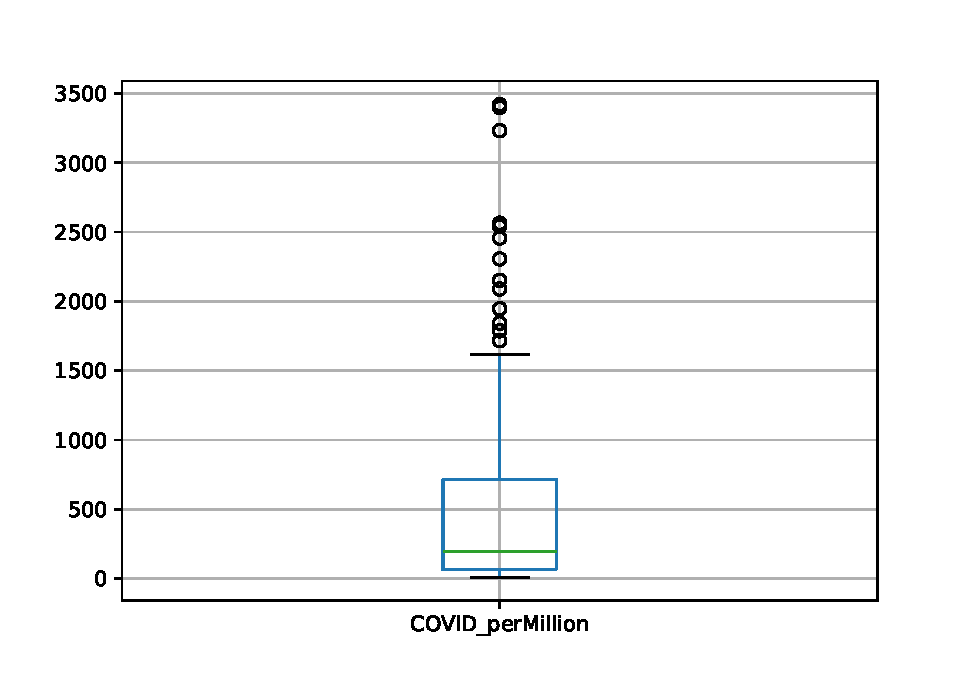
\includegraphics{_main_files/figure-latex/unnamed-chunk-121-13.pdf}

Na, ez már kb úgy néz ki, mint egy ``egészségesen'' jobbra elnyúló eloszlás doboz ábrája! :)

\section{Korrelációs elemzések data frame-ben}\label{korreluxe1ciuxf3s-elemzuxe9sek-data-frame-ben}

Nézzünk rá a numerikus adattípusú oszlopok közti korrelációs mátrixra. Egyedül a \textbf{Pop} és \textbf{COVID\_Cases} oszlopokat hagyjuk ki a vizsgálatból, mert azok abszolút és nem népességarányos adatok, így csalóka lenne őket szerepeltetni a korrelációs vizsgálatokban, hiszen ``triviálisan'' korrelálnak: nagyobb népességű országban nyilván több az összes esetszám. :)

Azt, hogy csak két oszlopot ne válasszunk ki egy data frame-ben úgy tudjuk elérni, hogy a data frame oszlopnevei közül egy \texttt{isin} metódussal kiválasztjuk a két kihagyandó oszlopot, majd az eredményt letagadjuk egy \texttt{\textasciitilde{}} jellel. Ezt a műveletet pedig beágyazzuk egy \texttt{loc} metódusba, és meg is vagyunk! :)

\begin{Shaded}
\begin{Highlighting}[]
\NormalTok{corona\_extended.loc[:,}\OperatorTok{\textasciitilde{}}\NormalTok{corona\_extended.columns.isin([}\StringTok{\textquotesingle{}COVID\_Cases\textquotesingle{}}\NormalTok{, }\StringTok{\textquotesingle{}Pop\textquotesingle{}}\NormalTok{])]}
\end{Highlighting}
\end{Shaded}

\begin{verbatim}
##                   Country  PopDensity  UrbanPop  COVID_perMillion
## 0             Afghanistan          60        25         55.769130
## 1                 Albania         105        63        268.608244
## 2                 Algeria          18        73         91.354724
## 5     Antigua and Barbuda         223        26        245.075514
## 6               Argentina          17        93         97.973762
## ..                    ...         ...       ...               ...
## 161               Ukraine          75        69        237.939741
## 162  United Arab Emirates         118        86       1261.930506
## 163        United Kingdom         281        83       2540.744366
## 164               Uruguay          20        96        185.103621
## 165            Uzbekistan          79        50         60.921678
## 
## [130 rows x 4 columns]
\end{verbatim}

Erre az oszlopaiban megvágott data frame-re pedig egy \texttt{corr} nevű metódust tudunk alkalmazni, ami megadja a numerikus oszlopok közti korrelációk mátrixszát. Figyeljünk még arra, hogy a \textbf{Country} oszlopot is ki kell szedni a korrelációszámításban érintett oszlopok közül, hiszen nem numerikus adattípusú, így a korrelációszámítás nem értelmezett rajta! Ennyire azért nem okos ez a pitonka kígyócska! :)

\begin{Shaded}
\begin{Highlighting}[]
\NormalTok{corona\_extended.loc[:,}\OperatorTok{\textasciitilde{}}\NormalTok{corona\_extended.columns.isin([}\StringTok{\textquotesingle{}Country\textquotesingle{}}\NormalTok{, }\StringTok{\textquotesingle{}COVID\_Cases\textquotesingle{}}\NormalTok{, }\StringTok{\textquotesingle{}Pop\textquotesingle{}}\NormalTok{])].corr()}
\end{Highlighting}
\end{Shaded}

\begin{verbatim}
##                   PopDensity  UrbanPop  COVID_perMillion
## PopDensity          1.000000 -0.051282          0.118036
## UrbanPop           -0.051282  1.000000          0.341160
## COVID_perMillion    0.118036  0.341160          1.000000
\end{verbatim}

A korrelációs mátrixból látszik, hogy az egymillió főre jutó COVID esetszám leginkább a városi népesség arányával függ össze, teljesen logikus módon: egyirányú, közepes erősségű a kapcsolat. A zsúfolt városi közösségi tereken, tömegközlekedésen könnyebb megfertőződni. :)

Nézzük is meg a kapcsolatot pontdiagramon! Teljesen úgy működik a pontdiagram is, mint pl. a korábbiakban a magyar adatokon látott területdiagram, csak a metódus neve nem \texttt{plot.area}, hanem \texttt{plot.scatter}. :)

\begin{Shaded}
\begin{Highlighting}[]
\NormalTok{corona\_extended.plot.scatter(x}\OperatorTok{=}\StringTok{"UrbanPop"}\NormalTok{, y}\OperatorTok{=}\StringTok{"COVID\_perMillion"}\NormalTok{)}
\end{Highlighting}
\end{Shaded}

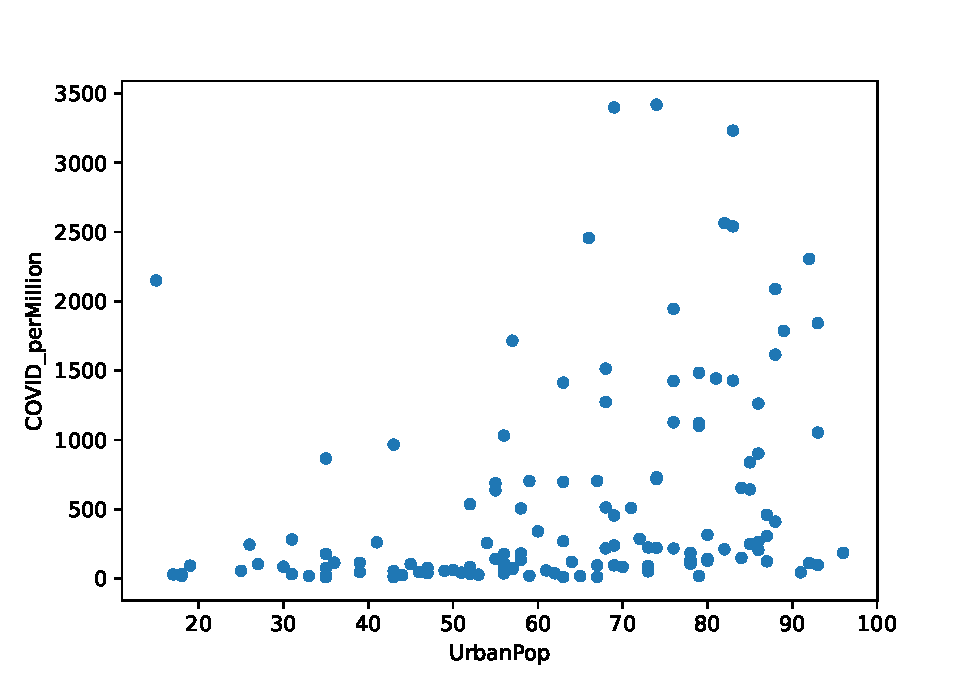
\includegraphics{_main_files/figure-latex/unnamed-chunk-124-15.pdf}

A pontdiagramon azt vehetjük észre, hogy az egymillió főre jutó COVID esetszám jobbra elnyúló eloszlása miatt jelenlévő felfelé kiugró értékek befolyásolják a két ismérv kapcsolatát. A kilógóan magas esetszámok miatt úgy tűnik, mintha az 500 alatti esetszámú országokban nem is lenne kapcsolat a két ismérv között.
A városi népesség arányával nincsenek ilyen problémák, mivel annak eloszlása közel szimmetrikus.

A két ismérv/oszlop eloszlásáról írtakat a hisztogramokon is meg lehet lesni.

Az egymillió főre jutó esetszám hisztogramja, ami elég jobbra elnyúló.

\begin{Shaded}
\begin{Highlighting}[]
\NormalTok{corona\_extended.COVID\_perMillion.hist()}
\end{Highlighting}
\end{Shaded}

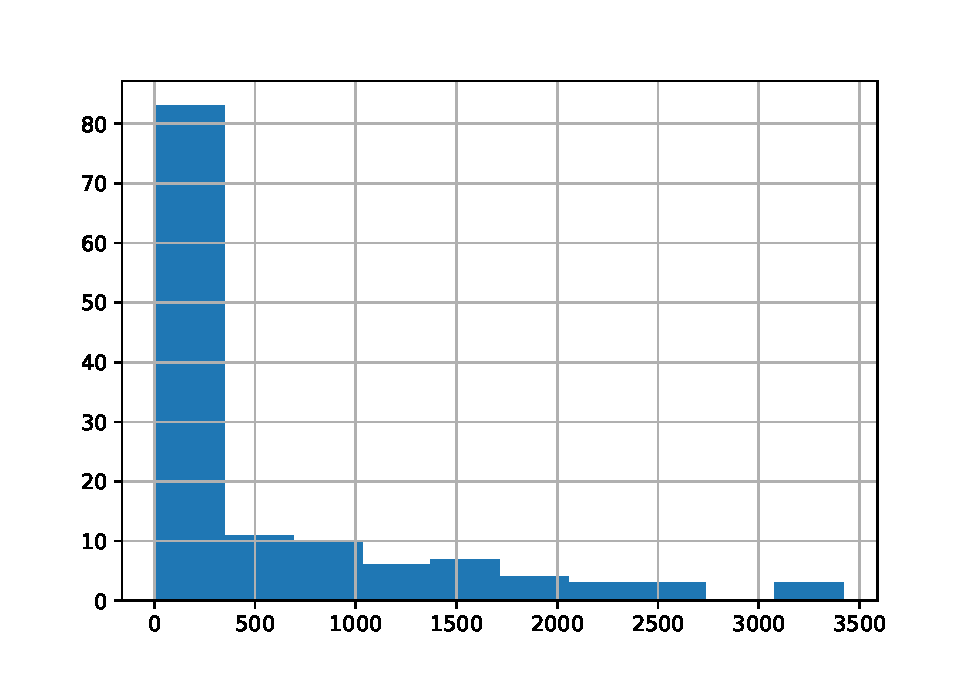
\includegraphics{_main_files/figure-latex/unnamed-chunk-125-17.pdf}

És a városi népesség arányáé, ami szimmetrikusabb egy fokkal, de némileg inkább balra elnyúló. A lényeg, hogy ezen nem segít a logaritmus. :)

\begin{Shaded}
\begin{Highlighting}[]
\NormalTok{corona\_extended.UrbanPop.hist()}
\end{Highlighting}
\end{Shaded}

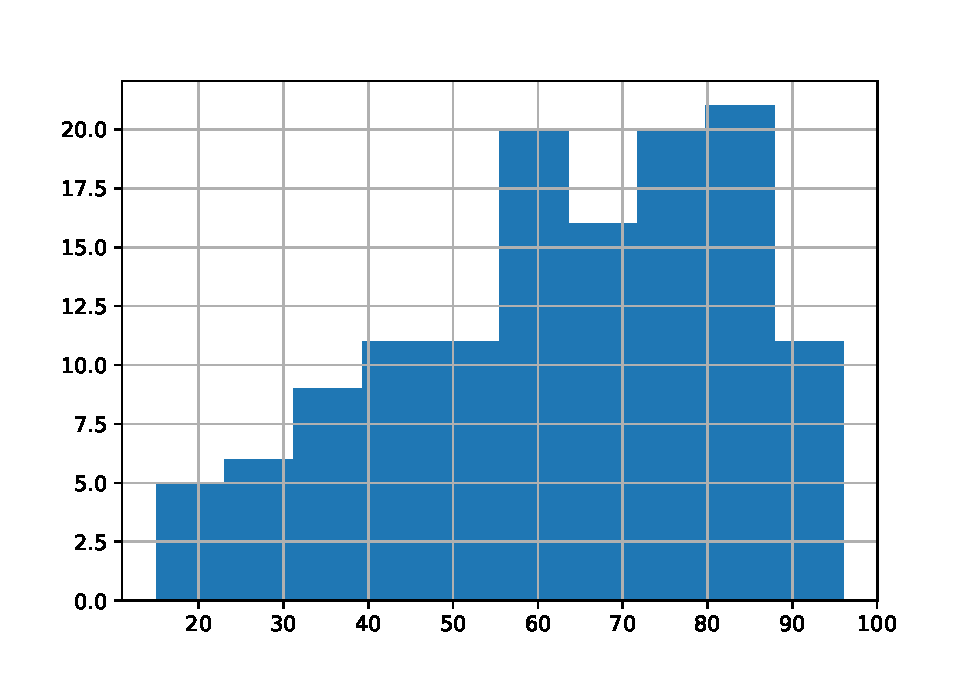
\includegraphics{_main_files/figure-latex/unnamed-chunk-126-19.pdf}

A kiugró értékek hatását, és az \textbf{eloszlás jobbra elnyúlóból közel szimmetrikussá alakítását logaritmussal} lehet elérni.

Készítsük is el a \textbf{COVID\_perMillion} oszlop természetes alapú logaritmusát egy új oszlopban a data frame-n belül.

\begin{Shaded}
\begin{Highlighting}[]
\NormalTok{corona\_extended[}\StringTok{\textquotesingle{}log\_COVID\_perMillion\textquotesingle{}}\NormalTok{] }\OperatorTok{=}\NormalTok{ np.log(corona\_extended[}\StringTok{\textquotesingle{}COVID\_perMillion\textquotesingle{}}\NormalTok{])}
\end{Highlighting}
\end{Shaded}

Ezek után lessünk rá az új oszlop hisztogramjára:

\begin{Shaded}
\begin{Highlighting}[]
\NormalTok{corona\_extended.log\_COVID\_perMillion.hist()}
\end{Highlighting}
\end{Shaded}

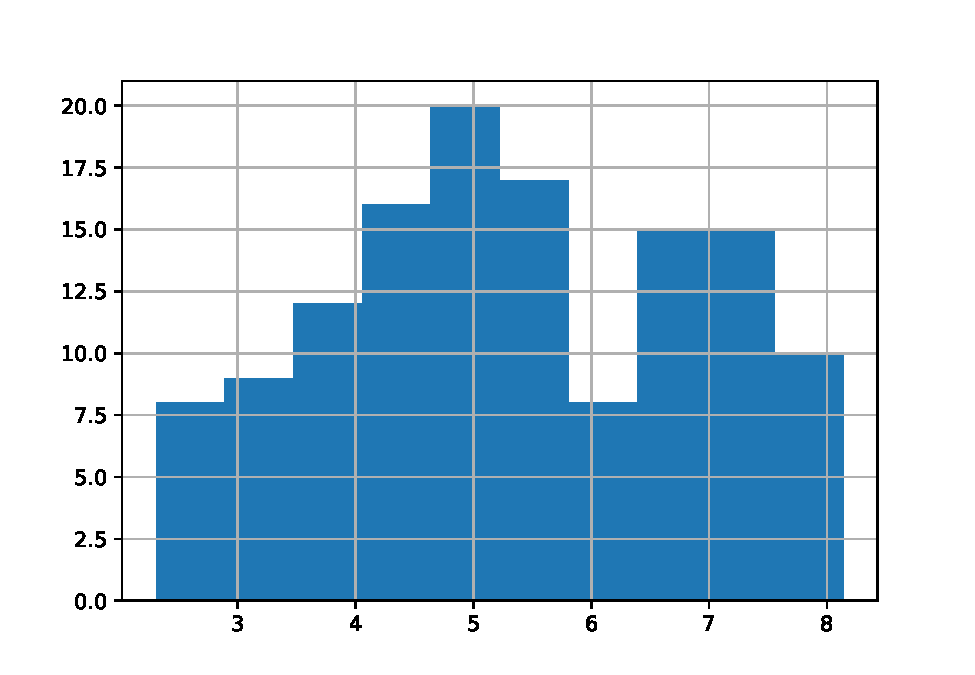
\includegraphics{_main_files/figure-latex/unnamed-chunk-128-21.pdf}

Sokkal szebb! :) Legalábbis szimmetria szempontjából biztos. Viszont van benne azért egy kétmóduszú jelleg. Ez azt jelenti, hogy van az országoknak egy jelentősebb csoportja, ahol emelkedettebb a népességarányos COVID esetszám, mint az országok többségében, akik az alacsonyabb értéktartományban lévő ``első móduszt'' adják.

A korreláció az esetszám logaritmusa és a városi népesség aránya között pedig feljavul. Abszolút értékben több, mint \(0.1\) egységet emelkedik a korreláció, ami nem elhanyagolható mértéjű javulás. :) Most a korrelációs mátrixból kivesszük a \textbf{PopDensity}-t is, hogy áttekinthetőbb legyen.

\begin{Shaded}
\begin{Highlighting}[]
\NormalTok{corona\_extended.loc[:,}\OperatorTok{\textasciitilde{}}\NormalTok{corona\_extended.columns.isin([}\StringTok{\textquotesingle{}Country\textquotesingle{}}\NormalTok{, }\StringTok{\textquotesingle{}COVID\_Cases\textquotesingle{}}\NormalTok{, }\StringTok{\textquotesingle{}Pop\textquotesingle{}}\NormalTok{, }\StringTok{\textquotesingle{}PopDensity\textquotesingle{}}\NormalTok{])].corr()}
\end{Highlighting}
\end{Shaded}

\begin{verbatim}
##                       UrbanPop  COVID_perMillion  log_COVID_perMillion
## UrbanPop              1.000000          0.341160              0.464379
## COVID_perMillion      0.341160          1.000000              0.826654
## log_COVID_perMillion  0.464379          0.826654              1.000000
\end{verbatim}

A korreláció abszolút értékében bekövetkezett javulás oka szépen látható a pontdiagramon: nincsenek már olyan durva outlierek a pontdiagramon. A pontokra nagyobb pontossággal illeszthető egy képzeletbeli egyenes a teljes tartományon nem csak az 500 feletti egymilliófőre vetített esetszámmal bíró országokban.

\begin{Shaded}
\begin{Highlighting}[]
\NormalTok{corona\_extended.plot.scatter(x}\OperatorTok{=}\StringTok{"UrbanPop"}\NormalTok{, y}\OperatorTok{=}\StringTok{"log\_COVID\_perMillion"}\NormalTok{)}
\end{Highlighting}
\end{Shaded}

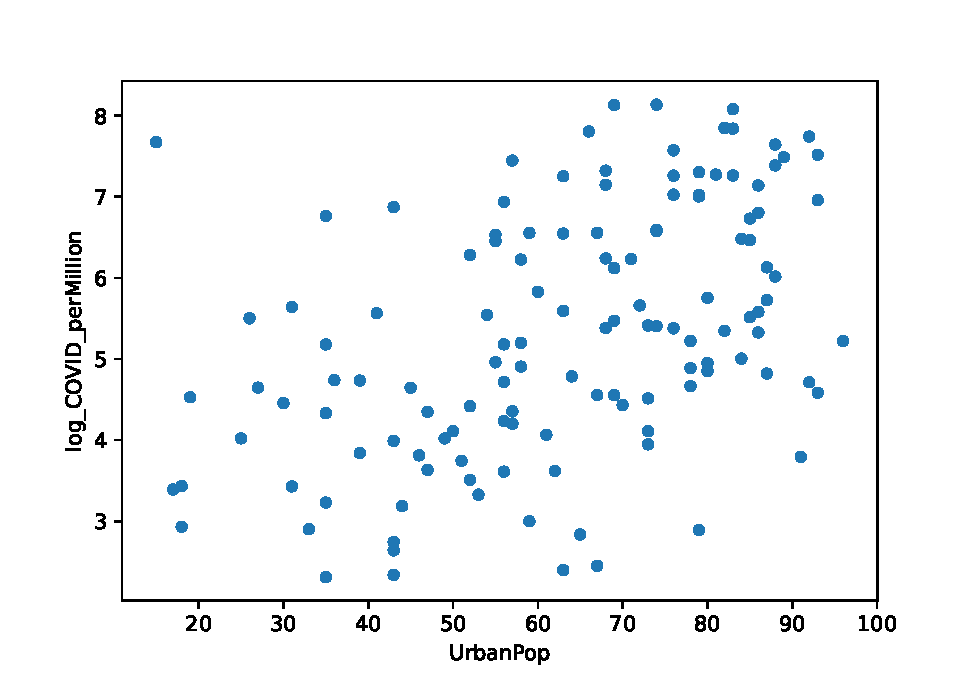
\includegraphics{_main_files/figure-latex/unnamed-chunk-130-23.pdf}

Annyit lehet látni, hogy van egy ország, aminek hatalmas az egymillió főre jutó COVID esetszáma az elég alacsony, \(20\%\) alatti városi népesség arányához képest. Jó lenne rájönni mi ez az ország!

Ehhez csináljunk egy olyan verziót az előző pontdiagramból, amin minden ponton szerepel, hogy az melyik országot jelöli.

Ennek elkészítéséhez felhasználunk egy \texttt{enumerate} névre hallgató függvényt. Ha ezt a függvényt ráeresztjük a \textbf{Country} oszlopra a data frame-ben, és az eredményt egy \texttt{for} ciklussal bejárjuk, akkor igazából két listát is bejárunk prhuzamosan:

\begin{itemize}
\tightlist
\item
  Egyet, ami az ország sorszámát mutatja a data frame-ben \(0\)-tól indexszelve. Ezt hívom én \texttt{sorszám}-nak.
\item
  A másik listában pedig az országnevek vannak. Ez a kódban \texttt{szöveg}-nek becézem.
\end{itemize}

Fontos, hogy a két listát bejáró változó neve teljesen tetszőleges, akár ``kismacska'' és ``gumimaci'' is lehetnének. :)

\begin{Shaded}
\begin{Highlighting}[]
\ControlFlowTok{for}\NormalTok{ sorszám, szöveg }\KeywordTok{in} \BuiltInTok{enumerate}\NormalTok{(corona\_extended.Country):}
   \BuiltInTok{print}\NormalTok{(sorszám)}
   \BuiltInTok{print}\NormalTok{(szöveg)}
\end{Highlighting}
\end{Shaded}

\begin{verbatim}
## 0
## Afghanistan
## 1
## Albania
## 2
## Algeria
## 3
## Antigua and Barbuda
## 4
## Argentina
## 5
## Armenia
## 6
## Australia
## 7
## Austria
## 8
## Azerbaijan
## 9
## Bahamas
\end{verbatim}

És ez így folytatódik tovább a data frame összes sorára, csak most ide nem íratom ki a több mint 100 értéket. :)

Na, ezt az \texttt{enumerate}-t használó \texttt{for} ciklust úgy hasznosítjuk, hogy először egy külön \texttt{fig} című objektumba elmentjk az alap pontdiagramos ábrát, amit az előbb is megcsináltunk.
Aztán elindítjuk ezt a \texttt{for} ciklust az \texttt{enumerate} alapján, és a cikluson belül használjuk a \texttt{fig} objektum \texttt{annotate} metódusát, ami a pontok feliratozását valósítja meg. A metódus paramétereiben megadom először, hogy az aktuális \texttt{szöveg}-et, azaz az országnevet rakja fel, mint felirat.
A következő paraméter, ami zárójelben van az csak optikai tuning. Ott azt csinálom, hogy az \(x,y\) koordinátáknak megfelelő oszlopok konkrét, pontdiagramon lévő koordinátáit kérdezem le az oszlopok \texttt{iat} tulajdonságában. Ez két lista, így mindig a \emph{sorszámadik} elemét nézem a cikluson belül. Ezen koordináták közül a diagram \(x\) tengelyét adó \textbf{UrbanPop}-ét eltolom \(0.05\)-tel. Így a pont felirata nem a pont középpontjában kezdődik, hanem attól \(0.05\) egységgel jobbra. Így olvashatóbb lesz a cucc. :) Nyilván a felirat \(y\) koordinátáját is tudnám itt szabályozni, és kedvem szerint fel-le rakni a felirat kezdőpontját, de erre itt nincs szükség, így az \texttt{annotate} paraméterben ezt a koordinátát csak csak változatlanul átadom.

Na, és lássuk is ezt a csodát működés közben! A kód végén egy \texttt{plt.show()} utasítással lehet a diagramot láthatóvá is tenni.

\begin{Shaded}
\begin{Highlighting}[]
\NormalTok{fig }\OperatorTok{=}\NormalTok{ corona\_extended.plot.scatter(x}\OperatorTok{=}\StringTok{"UrbanPop"}\NormalTok{, y}\OperatorTok{=}\StringTok{"log\_COVID\_perMillion"}\NormalTok{)}

\ControlFlowTok{for}\NormalTok{ sorszám, szöveg }\KeywordTok{in} \BuiltInTok{enumerate}\NormalTok{(corona\_extended.Country):}
\NormalTok{   fig.annotate(szöveg, (corona\_extended.UrbanPop.iat[sorszám]}\OperatorTok{+}\FloatTok{0.05}\NormalTok{, corona\_extended.log\_COVID\_perMillion.iat[sorszám]))}

\NormalTok{plt.show()}
\end{Highlighting}
\end{Shaded}

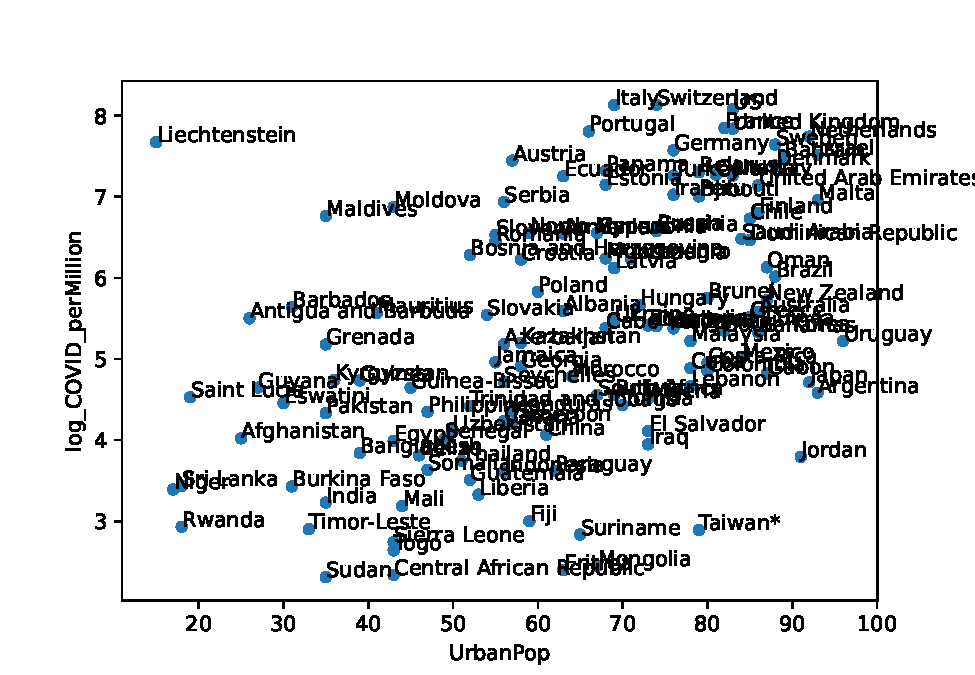
\includegraphics{_main_files/figure-latex/unnamed-chunk-133-25.pdf}

E voilá: a gyanús kis államunk a magas esetszámával a kis városi népesség arány ellenére \emph{Lichtenstein}! :) Érdekes észrevenni még, hogy pl. Taiwan elég jól áll: a városi népesség arányához képest elég alacsony az esetszáma! Magyarország, ha jól szemmelverjük, akkor látható, hogy gyakorlatilag pont a fő csapásirány közepén van kb: pont annyi nagyjából az esetszáma, amennyi a városi népesség aránya alapján ``lennie kéne''. :)

\section*{Gyakorló feladatok}\label{gyakorluxf3-feladatok}
\addcontentsline{toc}{section}{Gyakorló feladatok}

\begin{enumerate}
\def\labelenumi{\arabic{enumi}.}
\tightlist
\item
  Olvassuk be az index\_2019\_-\_pour\_import\_1\_1.csv nevű fájlt, és mentsük el a beolvasott adatokat egy \textbf{PressLiberty} nevű data frame-be!

  \begin{itemize}
  \tightlist
  \item
    Vigyázat! A fájlban tizedesvesszők vannak tizedes pont helyett! Használni kell a \texttt{read\_csv} függvény \texttt{decimal} paraméterét! Meg kell a paraméterben adni, hogy a tizedeshelyeket a \texttt{\textquotesingle{},\textquotesingle{}} karakter jelöli!
  \end{itemize}
\item
  A \textbf{PressLiberty} data frame-ből csak az angol országnév (\textbf{EN\_country}) és a 2019-es sajtószabadsági index (\textbf{Score 2019}) oszlopkra lesz szükségünk. A sajtószabadsági indexben az alacsonyabb érték jelent szabadabb sajtót egy országban. A többi változót töröljuk ki a data frame-ből!
\item
  A szűkített \textbf{PressLiberty} data frame oszlopainak neve legyen \textbf{Country} és \textbf{PressLiberty}!
\item
  Változtassuk meg az Egyesült Államok nevét ``\emph{United States}''-ről ``\emph{US}''-re a \textbf{PressLiberty} data frame-ben, hogy az összeköthető legyen a \textbf{corona\_extended} data frame-el az országneveken keresztül!
\item
  Inner Join művelet segítségével vezessük át a sajtószabadsági index vonatkozó adatokat a \textbf{corona\_extended} data frame-be!
\item
  Ábrázoljuk a \textbf{corona\_extended} data frame-ben a kapcsolatot a \textbf{log\_COVID\_perMillion} és \textbf{PressLiberty} ismérvek között pontdiagramon! Értelmezze röviden szövegesen is a kapcsolatot! Logikus-e a kapcsolat iránya?
\item
  Vizsgáljuk meg a \textbf{PressLiberty} eloszlását hisztogramon!
\item
  Adjuk hozzá a \textbf{corona\_extended} data frame-hez a \textbf{PressLiberty} logaritmusát \textbf{log\_PressLiberty} néven!
\item
  Nézzük meg a korrelációs mátrixot a \textbf{log\_COVID\_perMillion}, \textbf{PressLiberty} és \textbf{log\_PressLiberty} ismérvek között! Volt-e értelme a logaritmus alkalmazásának? Válaszát röviden indokolja!
\item
  Ábrázoljuk a \textbf{corona\_extended} data frame-ben a kapcsolatot a \textbf{COVID\_perMillion} logaritmusa és a \textbf{PressLiberty} logaritmusa között pontdiagramon! Az egyes pontokon szerepeljen az országok neve is!

  \begin{itemize}
  \tightlist
  \item
    Van-e olyan ország, amelyik a két ismérv kapcsolatát leíró általános tendenciához képest eltérően viselkedik? Válaszát röviden indokolja!
  \end{itemize}
\end{enumerate}

\section*{Gyakorló feladatok megoldása}\label{gyakorluxf3-feladatok-megolduxe1sa}
\addcontentsline{toc}{section}{Gyakorló feladatok megoldása}

\subsection*{1. feladat}\label{feladat}
\addcontentsline{toc}{subsection}{1. feladat}

\begin{Shaded}
\begin{Highlighting}[]
\NormalTok{PressLiberty }\OperatorTok{=}\NormalTok{ pd.read\_csv(}\StringTok{\textquotesingle{}index\_2019\_{-}\_pour\_import\_1\_1.csv\textquotesingle{}}\NormalTok{, decimal}\OperatorTok{=}\StringTok{\textquotesingle{},\textquotesingle{}}\NormalTok{)}
\NormalTok{PressLiberty.info()}
\end{Highlighting}
\end{Shaded}

\begin{verbatim}
## <class 'pandas.core.frame.DataFrame'>
## RangeIndex: 180 entries, 0 to 179
## Data columns (total 14 columns):
##  #   Column            Non-Null Count  Dtype  
## ---  ------            --------------  -----  
##  0   ISO               180 non-null    object 
##  1   Rank2019          180 non-null    int64  
##  2   FR_Country        180 non-null    object 
##  3   EN_country        180 non-null    object 
##  4   ES_country        180 non-null    object 
##  5   Score A           180 non-null    float64
##  6   Sco Exa           180 non-null    float64
##  7   Score 2019        180 non-null    float64
##  8   Progression RANK  180 non-null    int64  
##  9   Rank 2018         180 non-null    int64  
##  10  Score 2018        180 non-null    float64
##  11  Zone              180 non-null    object 
##  12  AR_country        180 non-null    object 
##  13  FA_country        180 non-null    object 
## dtypes: float64(4), int64(3), object(7)
## memory usage: 19.8+ KB
\end{verbatim}

\subsection*{2. feladat}\label{feladat-1}
\addcontentsline{toc}{subsection}{2. feladat}

\begin{Shaded}
\begin{Highlighting}[]
\NormalTok{PressLiberty }\OperatorTok{=}\NormalTok{ PressLiberty.loc[:,[}\StringTok{\textquotesingle{}EN\_country\textquotesingle{}}\NormalTok{, }\StringTok{\textquotesingle{}Score 2019\textquotesingle{}}\NormalTok{]]}
\NormalTok{PressLiberty.info()}
\end{Highlighting}
\end{Shaded}

\begin{verbatim}
## <class 'pandas.core.frame.DataFrame'>
## RangeIndex: 180 entries, 0 to 179
## Data columns (total 2 columns):
##  #   Column      Non-Null Count  Dtype  
## ---  ------      --------------  -----  
##  0   EN_country  180 non-null    object 
##  1   Score 2019  180 non-null    float64
## dtypes: float64(1), object(1)
## memory usage: 2.9+ KB
\end{verbatim}

\subsection*{3. feladat}\label{feladat-2}
\addcontentsline{toc}{subsection}{3. feladat}

\begin{Shaded}
\begin{Highlighting}[]
\NormalTok{PressLiberty.columns }\OperatorTok{=}\NormalTok{ [}\StringTok{\textquotesingle{}Country\textquotesingle{}}\NormalTok{, }\StringTok{\textquotesingle{}PressLiberty\textquotesingle{}}\NormalTok{]}
\NormalTok{PressLiberty.info()}
\end{Highlighting}
\end{Shaded}

\begin{verbatim}
## <class 'pandas.core.frame.DataFrame'>
## RangeIndex: 180 entries, 0 to 179
## Data columns (total 2 columns):
##  #   Column        Non-Null Count  Dtype  
## ---  ------        --------------  -----  
##  0   Country       180 non-null    object 
##  1   PressLiberty  180 non-null    float64
## dtypes: float64(1), object(1)
## memory usage: 2.9+ KB
\end{verbatim}

\subsection*{4. feladat}\label{feladat-3}
\addcontentsline{toc}{subsection}{4. feladat}

\begin{Shaded}
\begin{Highlighting}[]
\NormalTok{PressLiberty[}\StringTok{\textquotesingle{}Country\textquotesingle{}}\NormalTok{] }\OperatorTok{=}\NormalTok{ PressLiberty[}\StringTok{\textquotesingle{}Country\textquotesingle{}}\NormalTok{].replace(}\StringTok{\textquotesingle{}United States\textquotesingle{}}\NormalTok{, }\StringTok{\textquotesingle{}US\textquotesingle{}}\NormalTok{)}
\end{Highlighting}
\end{Shaded}

\subsection*{5. feladat}\label{feladat-4}
\addcontentsline{toc}{subsection}{5. feladat}

\begin{Shaded}
\begin{Highlighting}[]
\NormalTok{corona\_extended }\OperatorTok{=}\NormalTok{ pd.merge(corona\_extended, PressLiberty, how}\OperatorTok{=}\StringTok{\textquotesingle{}inner\textquotesingle{}}\NormalTok{, on}\OperatorTok{=}\StringTok{\textquotesingle{}Country\textquotesingle{}}\NormalTok{)}
\NormalTok{corona\_extended.info()}
\end{Highlighting}
\end{Shaded}

\begin{verbatim}
## <class 'pandas.core.frame.DataFrame'>
## RangeIndex: 115 entries, 0 to 114
## Data columns (total 8 columns):
##  #   Column                Non-Null Count  Dtype  
## ---  ------                --------------  -----  
##  0   Country               115 non-null    object 
##  1   COVID_Cases           115 non-null    int64  
##  2   Pop                   115 non-null    int64  
##  3   PopDensity            115 non-null    int64  
##  4   UrbanPop              115 non-null    int32  
##  5   COVID_perMillion      115 non-null    float64
##  6   log_COVID_perMillion  115 non-null    float64
##  7   PressLiberty          115 non-null    float64
## dtypes: float64(3), int32(1), int64(3), object(1)
## memory usage: 6.9+ KB
\end{verbatim}

\subsection*{6. feladat}\label{feladat-5}
\addcontentsline{toc}{subsection}{6. feladat}

\begin{Shaded}
\begin{Highlighting}[]
\NormalTok{corona\_extended.plot.scatter(x}\OperatorTok{=}\StringTok{"PressLiberty"}\NormalTok{, y}\OperatorTok{=}\StringTok{"log\_COVID\_perMillion"}\NormalTok{)}
\end{Highlighting}
\end{Shaded}

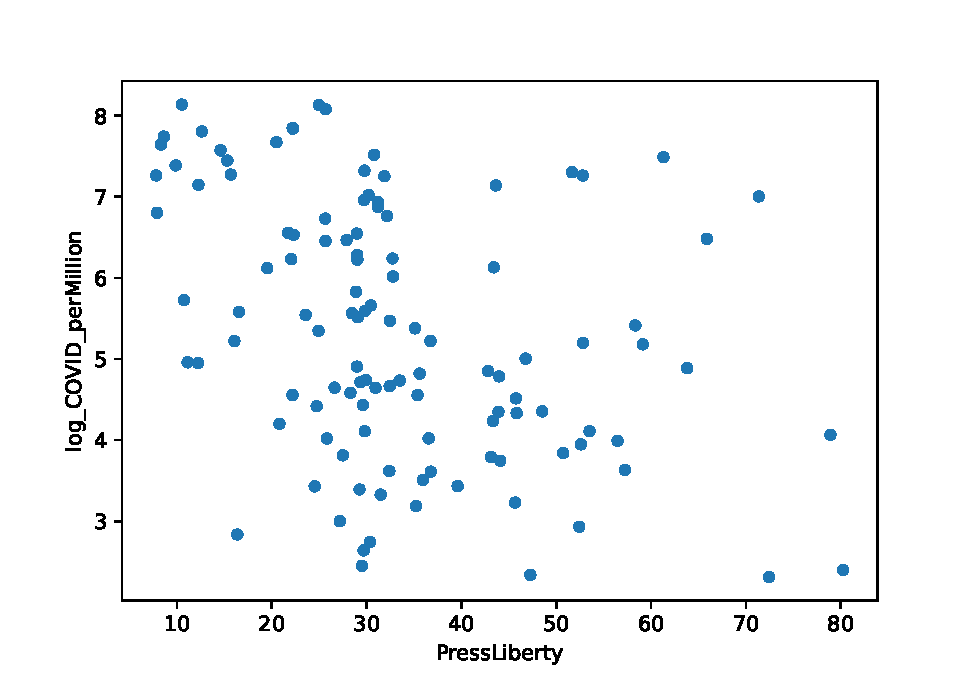
\includegraphics{_main_files/figure-latex/unnamed-chunk-139-27.pdf}

Úgy látszik, hogy a a kapcsolat ellentétes irányú: a sajtószabadsági index növekedésével jellemzően csökken az esetszám. Mivel a magasabb index jelenti a kevésbé szabad sajtót, így első olvasatra nem logikus a kapcsolat iránya: kevésbé szabad sajtóval rendelkező országokban kevesebb az esetszám egymillió főre nézve. De egy picit belegondolva lehet logikus a dolog: a szabadabb sajtóval rendelkező országok jellemzően gazdagabb országok is. Feltehetően ilyen országokban a COVID tesztelésre is több erőforrás jut.

\subsection*{7. feladat}\label{feladat-6}
\addcontentsline{toc}{subsection}{7. feladat}

\begin{Shaded}
\begin{Highlighting}[]
\NormalTok{corona\_extended.PressLiberty.hist()}
\end{Highlighting}
\end{Shaded}

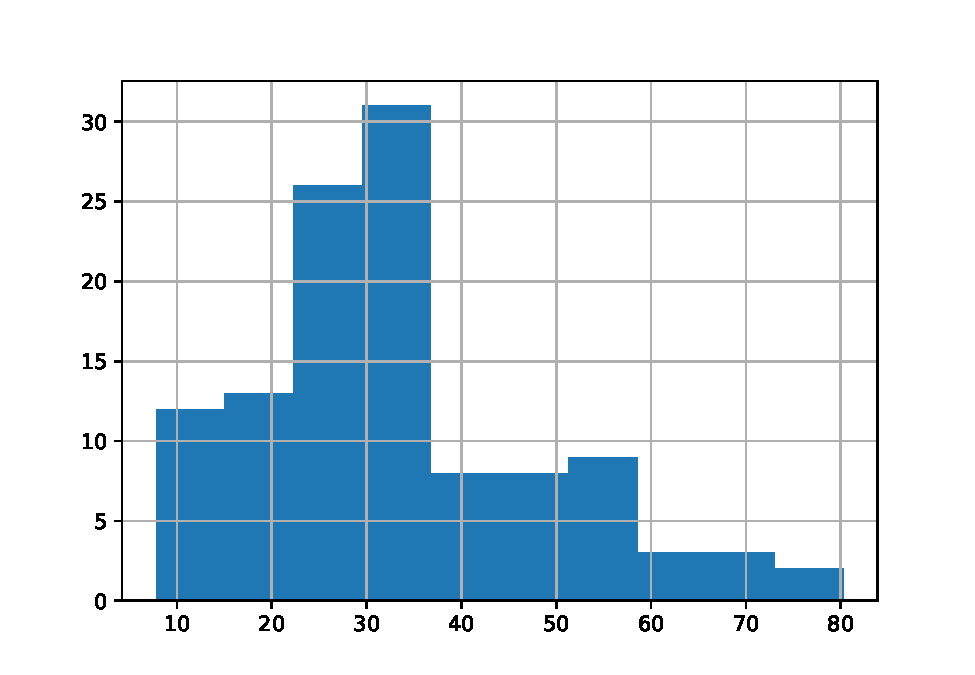
\includegraphics{_main_files/figure-latex/unnamed-chunk-140-29.pdf}

Az eloszlás némileg jobbra elnyúló, vannak felső irányban kiugró értékek. Érdemes lehet logaritmust alkalmazni az oszlopon.

\subsection*{8. feladat}\label{feladat-7}
\addcontentsline{toc}{subsection}{8. feladat}

\begin{Shaded}
\begin{Highlighting}[]
\NormalTok{corona\_extended[}\StringTok{\textquotesingle{}log\_PressLiberty\textquotesingle{}}\NormalTok{] }\OperatorTok{=}\NormalTok{ np.log(corona\_extended[}\StringTok{\textquotesingle{}PressLiberty\textquotesingle{}}\NormalTok{])}
\NormalTok{corona\_extended.info()}
\end{Highlighting}
\end{Shaded}

\begin{verbatim}
## <class 'pandas.core.frame.DataFrame'>
## RangeIndex: 115 entries, 0 to 114
## Data columns (total 9 columns):
##  #   Column                Non-Null Count  Dtype  
## ---  ------                --------------  -----  
##  0   Country               115 non-null    object 
##  1   COVID_Cases           115 non-null    int64  
##  2   Pop                   115 non-null    int64  
##  3   PopDensity            115 non-null    int64  
##  4   UrbanPop              115 non-null    int32  
##  5   COVID_perMillion      115 non-null    float64
##  6   log_COVID_perMillion  115 non-null    float64
##  7   PressLiberty          115 non-null    float64
##  8   log_PressLiberty      115 non-null    float64
## dtypes: float64(4), int32(1), int64(3), object(1)
## memory usage: 7.8+ KB
\end{verbatim}

\subsection*{9. feladat}\label{feladat-8}
\addcontentsline{toc}{subsection}{9. feladat}

\begin{Shaded}
\begin{Highlighting}[]
\NormalTok{corona\_extended.loc[:,[}\StringTok{\textquotesingle{}log\_COVID\_perMillion\textquotesingle{}}\NormalTok{, }\StringTok{\textquotesingle{}PressLiberty\textquotesingle{}}\NormalTok{, }\StringTok{\textquotesingle{}log\_PressLiberty\textquotesingle{}}\NormalTok{]].corr()}
\end{Highlighting}
\end{Shaded}

\begin{verbatim}
##                       log_COVID_perMillion  PressLiberty  log_PressLiberty
## log_COVID_perMillion              1.000000     -0.381829         -0.430291
## PressLiberty                     -0.381829      1.000000          0.944278
## log_PressLiberty                 -0.430291      0.944278          1.000000
\end{verbatim}

Volt értelme, a sajtószabadsági indexnek jobbra elnyúló az eloszlása, így a kilógó értékek hatását az egymillió főre vetített esetszámmal vett kapcsolatára tudta mérsékelni a logaritmus. Ez onnan látszódik, hogy a korreláció abszolút értékben \(0.05\) egységgel nőtt. Nem akkora a javulás, mint a városi népesség arányával vett korrelációnál tapasztaltuk, de azért észrevehető.

\subsection*{10. feladat}\label{feladat-9}
\addcontentsline{toc}{subsection}{10. feladat}

\begin{Shaded}
\begin{Highlighting}[]
\NormalTok{fig }\OperatorTok{=}\NormalTok{ corona\_extended.plot.scatter(x}\OperatorTok{=}\StringTok{"log\_PressLiberty"}\NormalTok{, y}\OperatorTok{=}\StringTok{"log\_COVID\_perMillion"}\NormalTok{)}

\ControlFlowTok{for}\NormalTok{ sorszám, szöveg }\KeywordTok{in} \BuiltInTok{enumerate}\NormalTok{(corona\_extended.Country):}
\NormalTok{   fig.annotate(szöveg, (corona\_extended.log\_PressLiberty.iat[sorszám]}\OperatorTok{+}\FloatTok{0.05}\NormalTok{, corona\_extended.log\_COVID\_perMillion.iat[sorszám]))}

\NormalTok{plt.show()}
\end{Highlighting}
\end{Shaded}

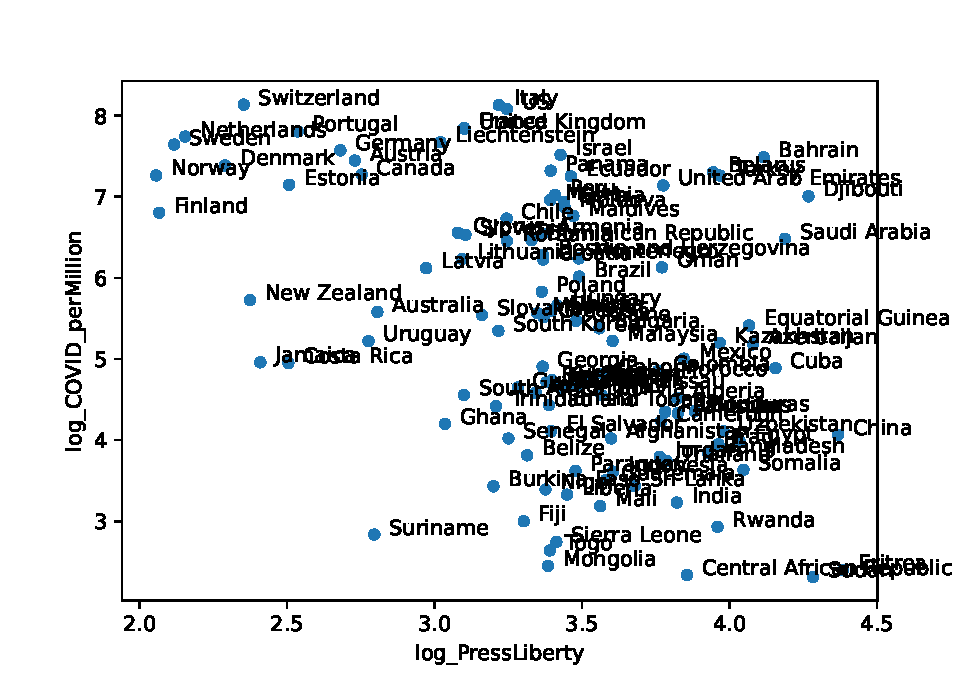
\includegraphics{_main_files/figure-latex/unnamed-chunk-143-31.pdf}

Úgy látszik, hogy pl. a dél-amerikai \emph{Suriname}-ben még a viszonylag rossz sajtószabadsági indexhez képest is kevés esettalálható egymillió főre. \emph{Bahrain}ben és \emph{Szaúd-Arábiában} viszont épp, hogy magas az esetszám a kevésbé szabad sajtó ellenére is. Itt lehet az olajvagyonból futja tesztelésre is \emph{úgymond}. :)

\chapter{Leíró Statisztika ismétlés és Valószínűségszámítás alapok}\label{leuxedruxf3-statisztika-ismuxe9tluxe9s-uxe9s-valuxf3szuxednux171suxe9gszuxe1muxedtuxe1s-alapok}

\section{Leíró statisztikai mutatók}\label{leuxedruxf3-statisztikai-mutatuxf3k}

A Stat. I. PTSD roham kiváltását kezdjük egy nagyon egyszerű kis ``Móricka példán''. Vizsgáljuk meg a TSLA.xlsx című táblában található adatokat, amik a \textbf{TESLA részvények napi záróárfolyam-változásai}t mutatják ki \textbf{dollárban} (\$) 2019 májusától 2020 májusáig.

Az Excel táblákat, amennyiben az adattáblánk első értéke az \emph{A1} cellában kezdődik és csak egy darab munkalapunk van, gond nélkül be lehet olvasni a \texttt{pandas} csomag \texttt{read\_excel} függvényével egy data frame-be. Több munkalap esetén a \texttt{read\_excel} függvény \texttt{sheet\_name} paraméterével tudjuk megadni a beolvasandó munkalap nevét stringként. Viszont ahhoz, hogy ez működőképes legyen fel kell még telepítenünk egy \texttt{openpyxl} című kiegészítő csomagot. A biztonság kedvéért ezzel a művelettel együtt rögtön importáljuk a statisztikai számításokhoz szükséges \texttt{numpy} és az ábrák megjelenítéséhez szükséges \texttt{matplotlib} csomagokat is.

\begin{Shaded}
\begin{Highlighting}[]
\NormalTok{pip install openpyxl}
\ImportTok{import}\NormalTok{ pandas }\ImportTok{as}\NormalTok{ pd}
\ImportTok{import}\NormalTok{ matplotlib.pyplot }\ImportTok{as}\NormalTok{ plt}
\ImportTok{import}\NormalTok{ numpy }\ImportTok{as}\NormalTok{ np}
\end{Highlighting}
\end{Shaded}

Ezek után pedig akkor jöhet az Excel beolvasás data frame-be!

\begin{Shaded}
\begin{Highlighting}[]
\NormalTok{Tesla }\OperatorTok{=}\NormalTok{ pd.read\_excel(}\StringTok{"TSLA.xlsx"}\NormalTok{)}

\NormalTok{Tesla.info()}
\end{Highlighting}
\end{Shaded}

\begin{verbatim}
## <class 'pandas.core.frame.DataFrame'>
## RangeIndex: 250 entries, 0 to 249
## Data columns (total 2 columns):
##  #   Column  Non-Null Count  Dtype         
## ---  ------  --------------  -----         
##  0   Dátum   250 non-null    datetime64[ns]
##  1   TESLA   250 non-null    float64       
## dtypes: datetime64[ns](1), float64(1)
## memory usage: 4.0 KB
\end{verbatim}

\begin{Shaded}
\begin{Highlighting}[]
\NormalTok{Tesla.head()}
\end{Highlighting}
\end{Shaded}

\begin{verbatim}
##        Dátum      TESLA
## 0 2019-05-07  -8.279998
## 1 2019-05-08  -2.220002
## 2 2019-05-09  -2.860000
## 3 2019-05-10  -2.459992
## 4 2019-05-13 -12.510009
\end{verbatim}

Láthatjuk, hogy két oszlopunk van: a dátum és a részvény árváltozása az adott napon az előző napi záróárfolyamhoz képest a \textbf{TESLA} oszlopban. Tehát 2019.05.07-én egy Tesla részvény kb. \(8.3\) dollárral ért kevesebbet a nap végére, mint amennyit 2019.05.06-án ért nap végén. Ellenben 05.13-án már \(12.5\) dollárral ér kevesebbet, mint előző nap, 05.12-én. Az \texttt{info} metódus alapján \(N=250\) napnyi ilyen adatunk van, ami nagyjából meg is egyezik egy évben a tőzsdei kereskedési napok számával.

Nos, az első öt vizsgált nap alapján nem lennék Elon Musk helyében, elég szép mínuszokat produkál a részvénye. De lássuk, hogy a leíró statisztikai mutatók mit árulnak el, hogyan is teljesített ez a csodacég a teljes vizsgált 1 éves időtartamban! Vessük át be a data frame \texttt{describe} metódusát!

\begin{Shaded}
\begin{Highlighting}[]
\NormalTok{Tesla.describe()}
\end{Highlighting}
\end{Shaded}

\begin{verbatim}
##                             Dátum       TESLA
## count                         250  250.000000
## mean   2019-11-02 15:56:09.600000    1.783920
## min           2019-05-07 00:00:00 -152.359986
## 25%           2019-08-05 06:00:00   -3.770005
## 50%           2019-10-31 12:00:00    1.420006
## 75%           2020-02-02 06:00:00    6.957486
## max           2020-05-01 00:00:00  129.429993
## std                           NaN   27.192611
\end{verbatim}

Lássuk hát milyen sztorit mesélnek a kiszámított mutatóink!

\begin{itemize}
\tightlist
\item
  Úgy látszik, hogy abszolút értékben a legnagyobb veszteség (\(-152\$\)) némileg nagyobb, mint a legnagyobb nyereség (\(+129\$\)).
\item
  Ugyanakkor, egy átlagos napon nagyjából jól járunk egy Tesla részvénnyel, mert kb. \(\mu=\bar{Y}=1.8\$\)-al növeli értékét.
\item
  Viszont, marha nagy a rizikó a rendszerben, mert a szórás (angolul \emph{standard deviation}, rövidítve \texttt{std}) alapján egy véletlenszerűen kiválasztott napon az árváltozás az \(\sigma=1.8\$\)-os átlagtól várhatóan \(\pm27.2\$\)-al térhet el. Azaz az árváltozások várható ingadozása az átlagos nyereségnek mintegy \(V=\frac{\sigma}{\mu}=\frac{27.2}{1.8}=15.1\)-szerese! (\emph{relatív szórás})
\item
  A medián árváltozás alapján azt mondhatjuk el, hogy a vizsgált időszakban a napok felében az elérhető maximális nyereség \(Me=1.42\$\), míg a napok másik felében a nyereség pedig legalább ennyi.
\item
  Az alsó kvartilis alapján a kereskedési napok legrosszabb \(\frac{1}{4}\)-ében a veszteség nagyobb, mint \(3.77\$\). Másképp: az árváltozás a napok negyedében kisebb, mint \(Q_1=-3.77\$\).
\item
  A napjaink legjobb \(25\%\)-ban pedig a nyereség legalább \(Q_3=6.96\$\)
\end{itemize}

Ha a fenti megállapításokat összenézzük, akkor arra juthatunk, hogy az \textbf{árváltozások eloszlása kb. szimmetrikus} lehet, egy \textbf{enyhe jobbra elnyúlással}. A \textbf{szimmetria mellett szól}, hogy az átlag nem nagyon tér el a mediántól (tehát a kilógó értékekre érzékeny átlag nem nagyon mozog el a kilógó értékekre robusztus felezőponttól), és a medián nagyjából egyenlő távolságra van az alsó és felső kvartilisektől (szóval az \(50\%\)-os pont a gyakoriságok szerint, értékekben is kb. a \(25\%\) és \(75\%\)-os pontok közepén helyezkedik el). Ellenben az \textbf{enyhe jobbra elnyúlás mellett érvel}, hogy azért mégis az átlag enyhén nagyobb mediánnál (tehát a felfelé kilógó értékek kicsit felfelé húzzák az átlagértéket a felezőponthoz képest), és a medián enyhén közelebb van az alsó kvartilishez, mint a felsőhöz (tehát az adatok többsége egy kicsit inkább az értéktartomány aljára koncentrálódik \(\rightarrow\) a kisebb értékből egy kicsit több van). De ezek tényleg nagyon enyhe eltérések. Sőt, \textbf{akár még a balra elnyúló eloszlás felé is lehet érvelni} azzal, hogy \(Q_3\) közelebb van a maximumhoz, mint \(Q_1\) a minimumhoz, tehát a \emph{felső} \(25\%\)-ban lévő értékek ``kevésbé húznak szét'', nem annyira kilógóak, mint az \emph{alsó} \(25\%\)-ban lévők.

\subsection{Hisztogram és Alakmutatók}\label{hisztogram-uxe9s-alakmutatuxf3k}

Az előző bekezdés dilemmáit leginkább \textbf{egy hisztogram segítségével tudnánk tisztázni}. A \textbf{hisztogramhoz} viszont szükségünk van egy \textbf{osztályközös gyakorisági táblára}, hiszen az árfolyamváltozások értékkészlete elég tág. Az osztályközöket vegyük egyenlő hosszúra. Ezek után már csak azt kell eldöntenünk, hogy \textbf{hány osztályközt} hozzunk létre! Ezt ugye Stat. I-ben legtöbbször a \textbf{``\(2^k\) szabállyal''} adtuk meg. Tehát az osztályközök száma a legkisebb olyan \(k\) szám, amire igaz az, hogy \(2^k \geq N\), ahol \(N\) az adataink elemszáma. Azt láttuk a \texttt{describe} eredményéből is pl., hogy \(N=250\). Ez alapján pedig a keresett \(k\) az \(8\) lesz, mert \(k=8:2^8 = 256 >250\), ám \(k=7:2^7=128 < 250\). Ha valaki ezt pitonul szeretné kiszámolni arra figyeljen, hogy ott a hatványozás jele a \texttt{**}.

\begin{Shaded}
\begin{Highlighting}[]
\DecValTok{2}\OperatorTok{**}\DecValTok{7}
\end{Highlighting}
\end{Shaded}

\begin{verbatim}
## 128
\end{verbatim}

\begin{Shaded}
\begin{Highlighting}[]
\DecValTok{2}\OperatorTok{**}\DecValTok{8}
\end{Highlighting}
\end{Shaded}

\begin{verbatim}
## 256
\end{verbatim}

Akkor hát nézzük meg a 8 egyenlő hosszú osztályközzel bíró gyakorisági tábla alapján készített hisztogramot.

\begin{Shaded}
\begin{Highlighting}[]
\NormalTok{Tesla.TESLA.hist(bins }\OperatorTok{=} \DecValTok{8}\NormalTok{)}
\end{Highlighting}
\end{Shaded}

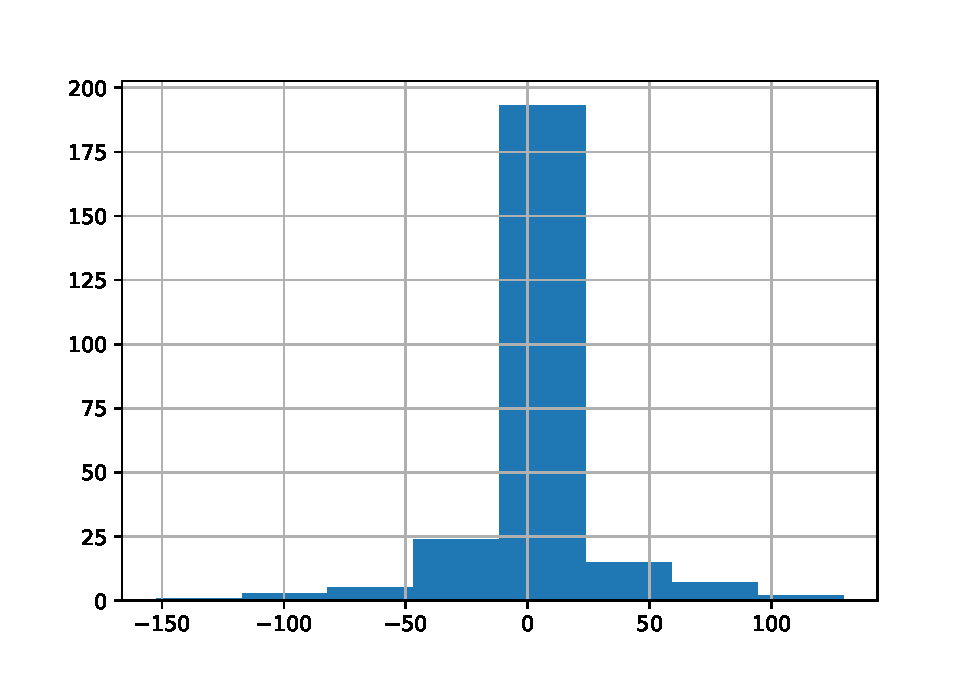
\includegraphics{_main_files/figure-latex/unnamed-chunk-149-33.pdf}

Nagyon szép, tényleg sac/kb szimmetrikus az eloszlás: középen, az \(1.8\$\)-os átlag körül csoportosul a legtöbb elem, és az ennél kisebb és nagyobb értékekből arányosan kevesebb van. Bár némileg kicsit csúcsosnak néz ki az eloszlás: a középső, átlag körüli, leggyakoribb értéktartományra koncentrálódik az adatok legnagyobb része, kb. \(190\) nap értéke az \(N=250\)-ből. Lássuk mi mondanak erről az \(\alpha_3, \alpha_4\) \textbf{alakmutatók}!

Az \(\alpha_3\) \textbf{aszimmetria mutató} Pythonban egy data frame oszlop \texttt{skew} metódusával, míg az \(\alpha_4\) \textbf{csúcsossági muató} az oszlop \texttt{skew} metódusával számítható.

\begin{Shaded}
\begin{Highlighting}[]
\NormalTok{Tesla.TESLA.skew()}
\end{Highlighting}
\end{Shaded}

\begin{verbatim}
## -0.5253045816998407
\end{verbatim}

\begin{Shaded}
\begin{Highlighting}[]
\NormalTok{Tesla.TESLA.kurt()}
\end{Highlighting}
\end{Shaded}

\begin{verbatim}
## 9.086855960563858
\end{verbatim}

Az \(\alpha_3\) értéke nagyon picit negatív, így enyhe balra elnyúlást jelez, de a hisztogram alapján látszik, hogy ez tényleg nagyon gyenge tendencia. Ez ugyebár abból adódik hogy \(Q_3\) közelebb van a maximumhoz, mint \(Q_1\) a minimumhoz. Tehát ezt a nagyon enyhe ``balra elnyúlást'' csak a maximum némileg kilógó viselkedése okozza, amire az \(\alpha_3\) ugyebár érzékeny, hiszen az átlag (\(\mu\)) alapján számoljuk őt ki (átlag körüli harmadik momentum).
Ellenben az \(\alpha_4=+9.09\)-es nagyon erősen pozitív értéke egyértelműen csúcsos eloszlás mutat, amit gyönyörűen látunk is a hisztogramon.

\subsection{Gyakorisági tábla lekérése}\label{gyakorisuxe1gi-tuxe1bla-lekuxe9ruxe9se}

Ha szeretnénk \textbf{megtekinteni a hisztogram mögött lakó osztályközös gyakorisági táblát}, akkor a dolgunk annyi, hogy a \texttt{hist} metódus helyett a \texttt{numpy} csomag \texttt{histogram} függvényével készítsük el a hisztogramot, és az eredményt mentsük el egy külön objektumba. A \texttt{histogram} függvény első paramétere az a data frame oszlop, amiből hisztogramot készítenénk, míg a második paramétere a \texttt{bins}, ami ugyan az, mint a data frame \texttt{hist} metódusában. Az elmentett eredményt data frame-é konvertáljuk a \texttt{pandas} csomag \texttt{DataFrame} függvénye segítségével, majd az eredményt transzponáljuk (alias 90 fokkal elforgatjuk) a data frame-k \texttt{transpose} metódusa segítségével.

\begin{Shaded}
\begin{Highlighting}[]
\NormalTok{gyaktábla }\OperatorTok{=}\NormalTok{ np.histogram(Tesla.TESLA, bins }\OperatorTok{=} \DecValTok{8}\NormalTok{)}
\NormalTok{gyaktábla }\OperatorTok{=}\NormalTok{ pd.DataFrame(gyaktábla).transpose()}
\NormalTok{gyaktábla}
\end{Highlighting}
\end{Shaded}

\begin{verbatim}
##        0           1
## 0    1.0 -152.359986
## 1    3.0 -117.136239
## 2    5.0  -81.912491
## 3   24.0  -46.688744
## 4  193.0  -11.464996
## 5   15.0   23.758751
## 6    7.0   58.982498
## 7    2.0   94.206246
## 8    NaN  129.429993
\end{verbatim}

Amit kaptunk az egy olyan tábla, aminek az \textbf{első oszlopa a gyakoriságok} értéke, míg a \textbf{második az adott osztályköz alsó határa}. Ezért van az utolsó sorban üres (\texttt{NaN}) érték, mert az ottani alsó határ az a vizsgált ismérvünk (árváltozásunk) maximuma, ami fölött természetesen már nincs érték.

Nevezzük át tartalmuknak megfelelően az oszlopokat, majd a \texttt{shift} metódus segítségével rakjuk be a táblába az adott osztályközök felső határait is. Itt a a \texttt{shift} metódusnál az alapelv, hogy az adott osztályköz felső határa nem más, mint a következő sor alsó határa.

\begin{Shaded}
\begin{Highlighting}[]
\NormalTok{gyaktábla.columns }\OperatorTok{=}\NormalTok{ [}\StringTok{\textquotesingle{}Gyakoriság\textquotesingle{}}\NormalTok{, }\StringTok{\textquotesingle{}AlsóHatár\textquotesingle{}}\NormalTok{]}
\NormalTok{gyaktábla.info()}
\end{Highlighting}
\end{Shaded}

\begin{verbatim}
## <class 'pandas.core.frame.DataFrame'>
## RangeIndex: 9 entries, 0 to 8
## Data columns (total 2 columns):
##  #   Column      Non-Null Count  Dtype  
## ---  ------      --------------  -----  
##  0   Gyakoriság  8 non-null      float64
##  1   AlsóHatár   9 non-null      float64
## dtypes: float64(2)
## memory usage: 276.0 bytes
\end{verbatim}

\begin{Shaded}
\begin{Highlighting}[]
\NormalTok{gyaktábla[}\StringTok{\textquotesingle{}FelsőHatár\textquotesingle{}}\NormalTok{] }\OperatorTok{=}\NormalTok{ gyaktábla.AlsóHatár.shift(}\OperatorTok{{-}}\DecValTok{1}\NormalTok{)}
\NormalTok{gyaktábla}
\end{Highlighting}
\end{Shaded}

\begin{verbatim}
##    Gyakoriság   AlsóHatár  FelsőHatár
## 0         1.0 -152.359986 -117.136239
## 1         3.0 -117.136239  -81.912491
## 2         5.0  -81.912491  -46.688744
## 3        24.0  -46.688744  -11.464996
## 4       193.0  -11.464996   23.758751
## 5        15.0   23.758751   58.982498
## 6         7.0   58.982498   94.206246
## 7         2.0   94.206246  129.429993
## 8         NaN  129.429993         NaN
\end{verbatim}

Na, ez egész pofás! Már csak annyi van, hogy rendezzük logikus sorrendbe az oszlopokat, és töröljük azt a nyomorult utolsó sort a \texttt{NaN}-nal.

\begin{Shaded}
\begin{Highlighting}[]
\NormalTok{gyaktábla }\OperatorTok{=}\NormalTok{ gyaktábla[[}\StringTok{\textquotesingle{}AlsóHatár\textquotesingle{}}\NormalTok{, }\StringTok{\textquotesingle{}FelsőHatár\textquotesingle{}}\NormalTok{, }\StringTok{\textquotesingle{}Gyakoriság\textquotesingle{}}\NormalTok{]]}
\NormalTok{gyaktábla }\OperatorTok{=}\NormalTok{ gyaktábla.drop(}\DecValTok{8}\NormalTok{, axis }\OperatorTok{=} \StringTok{"index"}\NormalTok{)}
\NormalTok{gyaktábla}
\end{Highlighting}
\end{Shaded}

\begin{verbatim}
##     AlsóHatár  FelsőHatár  Gyakoriság
## 0 -152.359986 -117.136239         1.0
## 1 -117.136239  -81.912491         3.0
## 2  -81.912491  -46.688744         5.0
## 3  -46.688744  -11.464996        24.0
## 4  -11.464996   23.758751       193.0
## 5   23.758751   58.982498        15.0
## 6   58.982498   94.206246         7.0
## 7   94.206246  129.429993         2.0
\end{verbatim}

Na, ez végre tök szépen olvasható! :) Láthatjuk például, hogy \(5\) olyan kereslkedési napunk volt a vizsgált időszakban, amikor az árfolyamváltozás \(-81\$\) és \(-46\$\) között volt, azaz a Tesla 46 és 81 dollár közti \emph{veszteséget} produkált ezen az 5 napon. Ellenben \(15\) napon \(23\$\) és \(58\$\) dollárt lehetett kaszálni egy Tesla részvényen. De amint a hisztogramon is látszott: a legtöbb, \(193\) napon az árfolyamváltozások a \(11\$\) \emph{veszteség} és a \(23\$\) \emph{nyereség} között (tehát úgy kb az \(1.8\$\) átlag környékén) ingadoztak.

\subsection{Gyakorisági tábla bővítése}\label{gyakorisuxe1gi-tuxe1bla-bux151vuxedtuxe9se}

Ha szeretnénk, akkor a \textbf{Relatív Gyakoriságokat} iis ki tudjuk számítani a táblába: ugyebár minden gyakoriságot leosztunk a teljes elemszámmal (\(N\)), ami a gyakoriságok összege. Ez Pythonban úgy néz ki, hogy a data frame gyakoriság oszlopát elosztjuk annak összegzett verziójával. Az összeg alias \texttt{sum} függvényt itt a \texttt{numpy} csomagból raboljuk el.

\begin{Shaded}
\begin{Highlighting}[]
\NormalTok{gyaktábla[}\StringTok{\textquotesingle{}RelatívGyak\textquotesingle{}}\NormalTok{] }\OperatorTok{=}\NormalTok{ gyaktábla.Gyakoriság }\OperatorTok{/}\NormalTok{ np.}\BuiltInTok{sum}\NormalTok{(gyaktábla.Gyakoriság)}
\NormalTok{gyaktábla}
\end{Highlighting}
\end{Shaded}

\begin{verbatim}
##     AlsóHatár  FelsőHatár  Gyakoriság  RelatívGyak
## 0 -152.359986 -117.136239         1.0        0.004
## 1 -117.136239  -81.912491         3.0        0.012
## 2  -81.912491  -46.688744         5.0        0.020
## 3  -46.688744  -11.464996        24.0        0.096
## 4  -11.464996   23.758751       193.0        0.772
## 5   23.758751   58.982498        15.0        0.060
## 6   58.982498   94.206246         7.0        0.028
## 7   94.206246  129.429993         2.0        0.008
\end{verbatim}

Szuper, így már láthatjuk, hogy az az \(5\) nap, amikor \(46\$\) és \(81\$\) közti \emph{veszteségünk} volt az az összes vizsgált napnak \(2\%\)-át jelenti.

Lehet \textbf{kumulálni} is a \texttt{cumsum} metódus segítségével. Számítsuk is ki így a \emph{kumulált relatív gyakoriságot}!

\begin{Shaded}
\begin{Highlighting}[]
\NormalTok{gyaktábla[}\StringTok{\textquotesingle{}KumRelatívGyak\textquotesingle{}}\NormalTok{] }\OperatorTok{=}\NormalTok{ gyaktábla.RelatívGyak.cumsum()}
\NormalTok{gyaktábla}
\end{Highlighting}
\end{Shaded}

\begin{verbatim}
##     AlsóHatár  FelsőHatár  Gyakoriság  RelatívGyak  KumRelatívGyak
## 0 -152.359986 -117.136239         1.0        0.004           0.004
## 1 -117.136239  -81.912491         3.0        0.012           0.016
## 2  -81.912491  -46.688744         5.0        0.020           0.036
## 3  -46.688744  -11.464996        24.0        0.096           0.132
## 4  -11.464996   23.758751       193.0        0.772           0.904
## 5   23.758751   58.982498        15.0        0.060           0.964
## 6   58.982498   94.206246         7.0        0.028           0.992
## 7   94.206246  129.429993         2.0        0.008           1.000
\end{verbatim}

Remek, az utolsó sorban ott a \(100\%\)-os kumulált relatív gyakoriság, ahogy kell, és azt is látjuk, hogy a vizsgált napjaink \(3.6\%\)-ban volt a \emph{veszteség} nagyobb, mint \(46\$\) (azaz az árváltozás kisebb, mint \(-46\$\)).

\subsection{Súlyozott átlag és szórás Pythonban}\label{suxfalyozott-uxe1tlag-uxe9s-szuxf3ruxe1s-pythonban}

Ha szeretnénk pl. \textbf{súlyozott átlagot számítani} a gyakorisági táblából azt is minden további nélkül megtehetjük! Kb. \textbf{pont ugyan úgy, mint Excelben}! Itt most a \emph{SZORZATÖSSZEG} függvény szerepét a \texttt{numpy}-féle \texttt{sum} függvény tölti be! Ezzel ugyan úgy \textbf{le tudjuk tükrözni a szummás statos képleteinket Pythonban, mint ahogy azt Excelben megtettük}.

Ugyebár a súlyozott átlaghoz két dolog kellenek, a \textbf{gyakoriságok}, alias \(f_i\)-k, és az \textbf{osztályközepek}, az \(Y_i\)-k. Előbbiek megvannak csak hozzáadom az \textbf{f\_i} jelölést az oszlop nevéhez, mígy az \(Y_i\)-ket kiszámolom, mint az osztály alsó és felső határának átlaga egy új \textbf{Y\_i} nevű oszlopba! Majd a data frame \textbf{oszlopnevekben mindig} '\_' \textbf{szimbólummal jelölöm az alsó indexet}!

\begin{Shaded}
\begin{Highlighting}[]
\NormalTok{gyaktábla }\OperatorTok{=}\NormalTok{ gyaktábla.rename(columns }\OperatorTok{=}\NormalTok{ \{}\StringTok{"Gyakoriság"}\NormalTok{:}\StringTok{"f\_i"}\NormalTok{\})}
\NormalTok{gyaktábla[}\StringTok{\textquotesingle{}Y\_i\textquotesingle{}}\NormalTok{] }\OperatorTok{=}\NormalTok{ (gyaktábla.AlsóHatár }\OperatorTok{+}\NormalTok{ gyaktábla.FelsőHatár) }\OperatorTok{/} \DecValTok{2}
\NormalTok{gyaktábla}
\end{Highlighting}
\end{Shaded}

\begin{verbatim}
##     AlsóHatár  FelsőHatár    f_i  RelatívGyak  KumRelatívGyak         Y_i
## 0 -152.359986 -117.136239    1.0        0.004           0.004 -134.748112
## 1 -117.136239  -81.912491    3.0        0.012           0.016  -99.524365
## 2  -81.912491  -46.688744    5.0        0.020           0.036  -64.300618
## 3  -46.688744  -11.464996   24.0        0.096           0.132  -29.076870
## 4  -11.464996   23.758751  193.0        0.772           0.904    6.146877
## 5   23.758751   58.982498   15.0        0.060           0.964   41.370625
## 6   58.982498   94.206246    7.0        0.028           0.992   76.594372
## 7   94.206246  129.429993    2.0        0.008           1.000  111.818119
\end{verbatim}

Nagyon jó, így mát tudom is alkalmazni a súlyozott átlag képletét: \[\mu=\bar{Y}=\frac{\sum_i{f_iY_i}}{N}\]

\begin{Shaded}
\begin{Highlighting}[]
\NormalTok{átlag }\OperatorTok{=}\NormalTok{ np.}\BuiltInTok{sum}\NormalTok{(gyaktábla.f\_i }\OperatorTok{*}\NormalTok{ gyaktábla.Y\_i) }\OperatorTok{/} \BuiltInTok{len}\NormalTok{(Tesla.TESLA)}
\NormalTok{átlag}
\end{Highlighting}
\end{Shaded}

\begin{verbatim}
## 4.456137313500011
\end{verbatim}

Remek, hát az osztályközepek használatával kicsit felélőttem a valóságnak (ami kb. \(1.8\$\) volt ugyebár), de hát ez ugye csak egy becslés. :)

A súlyozott szórást ugyan ezzel az elvvel ki lehet számolni pitonkával a képlete alapján: \[\sigma=\sqrt{\frac{\sum_i{f_i(Y_i-\bar{Y})^2}}{N}}\]

\begin{Shaded}
\begin{Highlighting}[]
\NormalTok{gyaktábla}
\end{Highlighting}
\end{Shaded}

\begin{verbatim}
##     AlsóHatár  FelsőHatár    f_i  RelatívGyak  KumRelatívGyak         Y_i
## 0 -152.359986 -117.136239    1.0        0.004           0.004 -134.748112
## 1 -117.136239  -81.912491    3.0        0.012           0.016  -99.524365
## 2  -81.912491  -46.688744    5.0        0.020           0.036  -64.300618
## 3  -46.688744  -11.464996   24.0        0.096           0.132  -29.076870
## 4  -11.464996   23.758751  193.0        0.772           0.904    6.146877
## 5   23.758751   58.982498   15.0        0.060           0.964   41.370625
## 6   58.982498   94.206246    7.0        0.028           0.992   76.594372
## 7   94.206246  129.429993    2.0        0.008           1.000  111.818119
\end{verbatim}

\begin{Shaded}
\begin{Highlighting}[]
\NormalTok{szórás }\OperatorTok{=}\NormalTok{ np.sqrt(np.}\BuiltInTok{sum}\NormalTok{(gyaktábla.f\_i }\OperatorTok{*}\NormalTok{ (gyaktábla.Y\_i}\OperatorTok{{-}}\NormalTok{átlag)}\OperatorTok{**}\DecValTok{2}\NormalTok{) }\OperatorTok{/} \BuiltInTok{len}\NormalTok{(Tesla.TESLA))}
\NormalTok{szórás}
\end{Highlighting}
\end{Shaded}

\begin{verbatim}
## 27.048902512450574
\end{verbatim}

Na, ezt már nem lőttük annyira mellé a valós \(27.19\$\)-hez képest. Ezzel meg is vagyunk, juppí! :)

\section{A normális eloszlás és sűrűségfüggvénye}\label{a-normuxe1lis-eloszluxe1s-uxe9s-sux171rux171suxe9gfuxfcggvuxe9nye}

Térjünk vissza a Tesla részvényárfolyamok hisztogramjához. Most rajzoljuk ki úgy a cuccot, hogy a \texttt{hist} metóduson bekapcsolunk egy \texttt{density\ =\ True} beállítást. Ez úgy rajzolja ki a hisztogramot, hogy az \(y\) tengelyen nem a gyakoriságok jelennek meg, hanem azoknak egy úgy skálázott verziója, hogy a maximum érték az adott osztály osztályközepének és a körülötte lévő \(\pm 2\) érték együttes relatív gyakoriságával arányos. Mivel egy konkrét érték gyakorisága itt most \(\frac{1}{250}\), így a maximum érték egy jó alacsony szám lesz az \(y\) tenegelyen, egész konkrétan kb. \(\frac{5}{250}=0.02\). A többi oszlop magassága az eredeti gyakoriságok szerint legyártott hisztogram alapján van belőve ehhez a maximum értékhez. Szóval, a hisztogram alakja nem változik, csak az \(y\) tengely van máshogy beskálázva.

\begin{Shaded}
\begin{Highlighting}[]
\NormalTok{Tesla.TESLA.hist(bins }\OperatorTok{=} \DecValTok{8}\NormalTok{, density }\OperatorTok{=} \VariableTok{True}\NormalTok{)}
\end{Highlighting}
\end{Shaded}

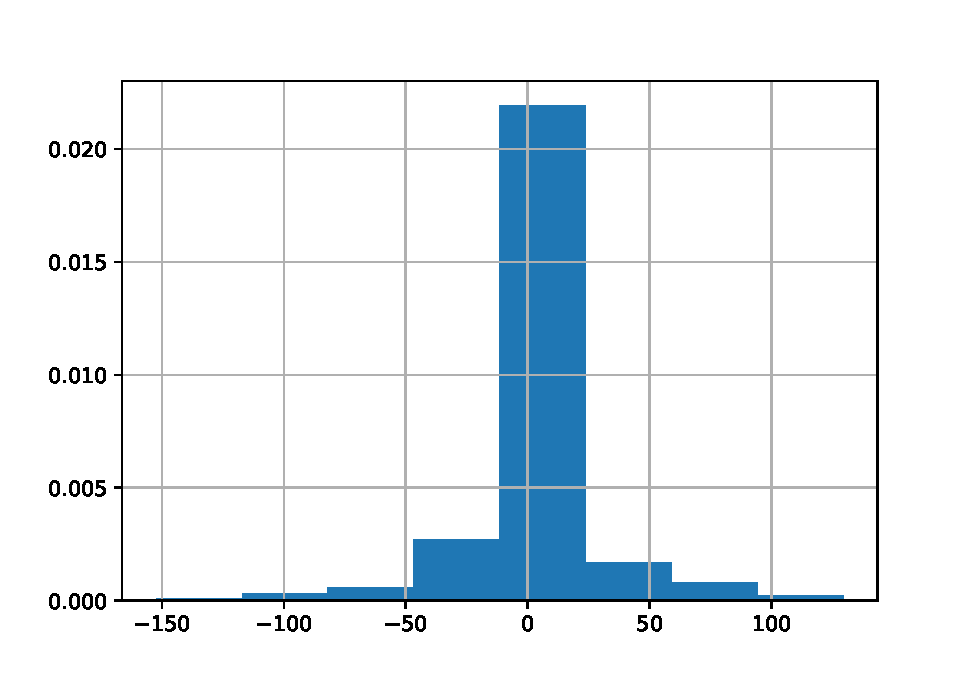
\includegraphics{_main_files/figure-latex/unnamed-chunk-159-35.pdf}

Meg is van a csodaszépen szimmetrikus eloszlást mutató hisztogramunk.
Ezen a ``\emph{relatív gyakoriságos}'' hisztogramon azt a gondolatot kell most elképzelni, hogy milyen alakzatot kapunk, ha \textbf{az oszlopokat összekötjük egy folytonos vonallal}.
Nos, nem kell sokat fantáziálni, a vonnallal összekötés az \textbf{alábbi alakzathoz hasonló függvényt eredményez}:

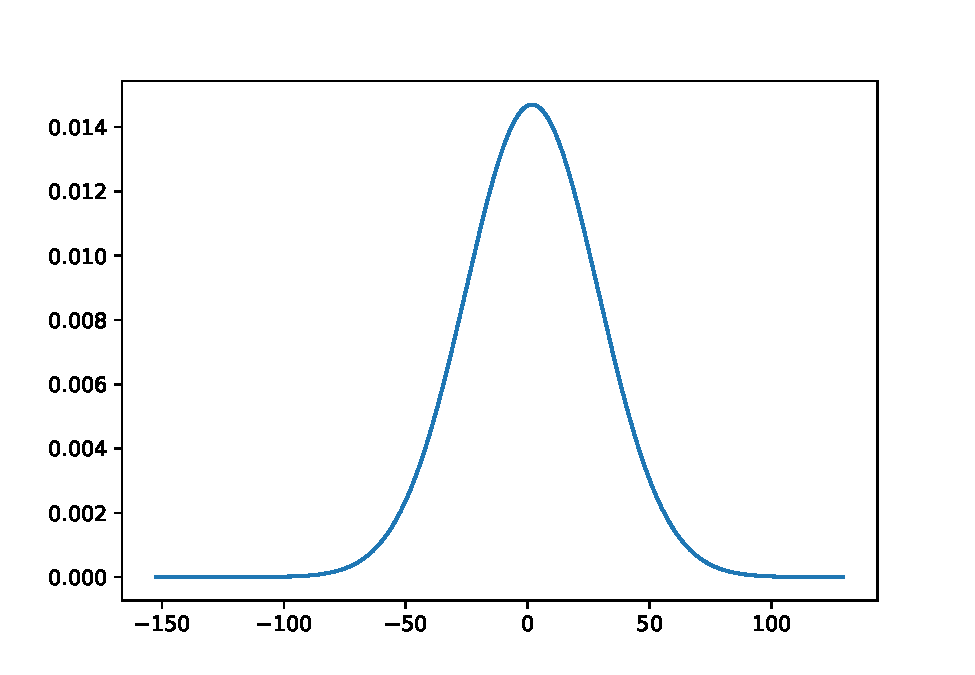
\includegraphics{_main_files/figure-latex/unnamed-chunk-160-37.pdf}

Amit itt látunk az nem más, mint \textbf{egy normális eloszlás sűrűségfüggvénye}. Sőt, pontosítok is, ez \textbf{az alakzat egy \(\mu=1.8\) átlagú és \(\sigma=27.19\) szórású normális eloszlás sűrűségfüggvénye, hiszen ennyi volt a Tesla árfolyamváltozások adatsorának átlaga és szórása, aminek a hisztogramja alapján gondolatban kirajzoltuk ezt a sűrűségfüggvényt}. Ezt ilyenkor úgy szoktuk szakszerűen mondani, hogy amit látunk az egy \(N(1.8,27.19)\) eloszlás sűrűségfüggvénye. Általánosságban egy normális eloszlásra pedig \(N(\mu, \sigma)\) jelöléssel hivatkozunk.

Miért is van ez így? Mivel \textbf{azt, hogy konkrétan milyen egy normális eloszlású sűrűségfüggvény alakja, meghatározza, hogy mennyi az adatsor átlaga és szórása, amire ezt a sűrűségfüggvényt úgymond illeszteni szeretnénk}. Azt, hogy hogyan az alábbi kis interaktív ábra szemlélteti:

Amúgy a normális eloszlás sűrűségfüggvényének hozzárendelési \(f(x)\) utasítása \(\mu\) átlag és \(\sigma\) szórás függvényében az alább alakot ölti.\[f(x)=\frac{1}{\sigma\sqrt{2\pi}}e^{-\frac{1}{2}\left(\frac{x-\mu}{\sigma}\right)^2}\]

Mielőtt szörnyet halunk az Analízis emlékek által kiváltott PTSD-ben, megnyugtatok mindenkit: erre a épletre igazából nekünk nem lesz szükségünk, de egyszer nem árt ha látjuk a függvény mögötti képletet is. :)

\subsection{A sűrűségfüggvény használata}\label{a-sux171rux171suxe9gfuxfcggvuxe9ny-hasznuxe1lata}

No, de ``\emph{Mit adtak nekünk a rómaiak?}'' Azaz jogosan kérdezhetjük, hogy mire tudjuk használni ezt a sűrűségfüggvényt? Első és legfontosabb funkciója, hogy ha a függvény \(f(x)\) formulájába behelyettesítek egy \(x\) értéket, akkor megkapom, hogy \textbf{mi a valószínűsége, hogy az \(Y\) adatsoromból egy véletlenszerűen kihúzott \(Y_i\) érték az \(x\)-et vesz fel}. Magyarul \(f(x)=P(Y_i=x)\).
Most itt egy picit \textbf{pontatlan voltam}. Ugyanis nem egész pontosan a \(Y_i=x\) esemény valószínűségét kapjuk meg, mert nagy értékkészlet esetén az gyakorlatilag \(0\) lenne. Gondoljunk bele: annak a valószínűsége, hogy a Tesla napi árváltozása éppen pont \(2.760009\$\) az tényleg gyakorlatilag \(0\), de a valóságban pont ennyi volt a cucc 2019. május 23-án. Szóval, abszolút nem lehetetlen\ldots{} Azaz, egész pontosan az \(f(x)\) sűrűségfüggvény érték \emph{arányos} a \(P(x<Y_i<x+ \epsilon)\) esemény valószínűségével, ahol az \(\epsilon\) egy \emph{nagyon kicsi} szám. Konkrétan, azt mondhatjuk, hogy \(P(x<Y_i<x+ \epsilon)=f(x) \times \epsilon\). Tehát, annak a valószínűsége, hogy a random módon kihúzott \(Y_i\) értékünk az \(x\)-nek egy \emph{nagyon kicsi}, \(\epsilon\)-nyi környezetébe esik, arányos az \(f(x)\) sűrűségfüggvény értékével. Ha nagyobb ez a valószínűség, akkor nagyobb a sűrűségfüggvény érték is, és fordítva. Szóval, annyi biztosan elmondható, hogy amelyik \(x\) pontnak nagyobb az \(f(x)\) sűrűségfüggvény értéke, annak nagyobb is a bekövetkezési valószínűsége, ha véletlenszerűen kiválasztok egy tetszőleges \(Y_i\) értéket. Csak a két dolog (sűrűségfüggvény és valószínűség) nem ugyan az, az eltérésük egy \(\epsilon\) szorzó.
Emiatt van az is, hogy a Pythonban a \texttt{hist} metódus \texttt{density\ =\ True} beállítással a relatív gyakoriságokat a legnagyobb gyakoriságú \(Y_i\) osztályközép \(\pm 2\) környezet relatív gyakorisága alapján mutatja meg a hisztogram \(y\) tengelyén.
De most nekünk \textbf{szemléletes szempontból teljesen jó lesz, ha úgy gondolunk a helyettesítési értékre \(x\) helyen, mint az \(x\) érték bekövetkezési valószínűsége}. Azaz, mi a \(f(x)=P(Y_i=x)\) értelmezéssel megyünk tovább.

Ez alapján, ha meg akarjuk tudni, hogy mennyi a valószínűsége, hogy a Tesla egy random napi árfolyamváltozása épp a 2019. május 23-i kb. \(2.76\$\)-al lesz egyenlő, akkor ahhoz az alábbi csodát kell kiszámolni.\[P(Y_i=2.76)=f(2.76)=\frac{1}{27.19\sqrt{2\pi}}e^{-\frac{1}{2}\left(\frac{2.76-1.8}{27.19}\right)^2}\]

Hiszen azt tudjuk, hogy a megfigyelt kereskedési napok alapján az árváltozások átlaga \(\mu=1.8\$\) és szórása \(\sigma=27.19\$\).

Na, ezt számolja ki kézzel az, aki papíron tanulja a Stat. II-t. :) Mi Pythonban be tudjuk vetni a \texttt{scipy} csomag \texttt{stats} névterében található függvényeket egy ilyen normális eloszlás sűrűségfüggvény-érték kiszámítására!

Telepítsuk a csomagot és importáljuk a szükséges függvényeket egy \texttt{stats} névtérbe. A \textbf{csomagot nagyon sokat fogjuk hazsnálni a félév során}, és egy szép alapos dokumentációja van. Érdemes olvasgatni! :)

\begin{Shaded}
\begin{Highlighting}[]
\NormalTok{pip install scipy}
\ImportTok{import}\NormalTok{ scipy.stats }\ImportTok{as}\NormalTok{ stats}
\end{Highlighting}
\end{Shaded}

Majd a névtér \texttt{norm.pdf} függvénye segítségével számoljuk ki a keresett valószínűséget! A függvény \textbf{3 paraméterrel operál, ebben a sorrendben: \(x, \mu, \sigma\).} Annyit érdemes megjegyezni, hogy a függvény a \(\mu\) átlagot location-nek, azaz \texttt{loc}-nak, míg a \(\sigma\) szórást \texttt{scale}-nek nevezi a saját kis nyelvjárásában. A függvény neve pedig az angol \emph{probability density function}-ból (valószínűségi sűrűségfüggvény) rövidül \emph{pdf}-nek.

\begin{Shaded}
\begin{Highlighting}[]
\NormalTok{mű }\OperatorTok{=} \FloatTok{1.8}
\NormalTok{szigma }\OperatorTok{=} \FloatTok{27.19}
\NormalTok{stats.norm.pdf(x }\OperatorTok{=} \FloatTok{2.76}\NormalTok{, loc }\OperatorTok{=}\NormalTok{ mű, scale }\OperatorTok{=}\NormalTok{ szigma)}
\end{Highlighting}
\end{Shaded}

\begin{verbatim}
## 0.014663247477553697
\end{verbatim}

Szuper, ez azt jelenti, hogy kb. \(1.466\%\) a valószínűsége annak, hogy egy véletlenszerű napon egy Tesla részvénnyel \(2.76\$\)-t lehet kaszálni.

Ezen a ponton \textbf{érdemes belegondolni, hogyan is reagált a sűrűségfüggvény a szórás növekedésére\ldots ellaposodott!} Na, ez most teljesen érthetővé válik, hiszen \textbf{ha a szórás nő}, az azt jelenti, hogy a \textbf{szélsőségesen magas vagy alacsony \(Y_i\) értékek bekövetkezési valószínűsége is megnő}\ldots és ha a \textbf{függvény \(f(x)\) értéke épp ezekkel a \(P(Y_i=x)\) valószínűségekkel egyenlő}, akkor épp a \textbf{két szélen fog ``meghízni'' a függvény képe}, azaz \textbf{ellaposodik}!

\subsection{A sűrűségfüggvény integrálja}\label{a-sux171rux171suxe9gfuxfcggvuxe9ny-integruxe1lja}

Azért láthatjuk, hogy egy konkrét érték bekövetkezési valószínűsége, alapól nem valami nagy, épp azért, amit fejtegettünk korábban is: az árváltozások értékkészlete elég nagy, egy konkrét érték (vagy annak kis környezetének) bekövetkezési valószínűsége elég kicsi.
Emiatt nem is ezt a kérdést szoktuk általában feltenni a sűrűségfüggvénynek, hanem pl. azt, hogy \textbf{mi a valószínűsége annak, hogy egy véletlenszerűen kihúzott \(Y_i\) érték egy előre megadott \(x\) érték alatt helyezkedik el}? Tehát a \(P(Y_i < x)\) valószínűséget keressük általában.
Ez pedig nem más, mint a \textbf{sűrűségfüggvény \(x\) alatti részének területe}, vagyis a \(\int_{-\infty}^x{f(x)}dx\) improprius integrál.

Na, ha a sűrűségfüggvény helyettesítési értékét nem akartuk kézzel-lábbal kiszámolni, akkor ezt az improprius integrált meg pláne nem!
Szerencsére, \textbf{van erre is beépített függvényünk} a \texttt{scipy} csomagban \texttt{norm.cdf} néven. Ugyan úgy működik, mint a \texttt{norm.pdf}, 3 paramétere van, ugyan abban a sorrendben: \texttt{x,\ loc,\ scale}, csak a \(P(Y_i < x)\)-et számítja ki, nem a \(P(Y_i = x)\)-t a megadott átlagú és szórású normális eloszlás sűrűségfüggvény alapján. A függvény neve az angol \emph{cumulative density function}-ból (kumulált sűrűségfüggvény) rövidül \emph{cdf}-nek. Ha belegondolunk ez logikus, hiszen felösszegezzük (azaz felkumuláljuk) az egyes \(Y_i\) elemek bekövetkezési valószínűségét \(-\infty\)-től \(x\)-ig.

Lássuk akkor hát pl., hogy mennyi a valószínűsége, hogy egy véletlenszerűen kiszúrt kereskedési napon a Teslával \(82\$\)-nál nagyobb \emph{veszteségünk} lesz! Tehát, a \(P(Y_i<-82)\) valószínűséget keressük.

\begin{Shaded}
\begin{Highlighting}[]
\NormalTok{stats.norm.cdf(x }\OperatorTok{=} \OperatorTok{{-}}\DecValTok{82}\NormalTok{, loc }\OperatorTok{=}\NormalTok{ mű, scale }\OperatorTok{=}\NormalTok{ szigma)}
\end{Highlighting}
\end{Shaded}

\begin{verbatim}
## 0.0010280208392538434
\end{verbatim}

Ez pedig a korábban megadott \(\mu\) átlaggal és \(\sigma\) szórással nem más, mint kb. \(0.1\%\). Szóval, szerencsére egy jó kicsi érték! :)

Természetesen ha egy \(x\) érték alá esési valószínűségét ki tudjuk számolni, akkor az \(x\) felé esés valószínűségét már gyerekjáték kiszámolni, hiszen \textbf{a ``felé esés'' az ``alá esés'' komplementer eseménye}, azaz \(P(Y_i>x)=1-P(Y_i<x)\). Szemléletesen pedig itt a \textbf{sűrűségfüggvény \(x\) feletti részének területét} számoljuk ki.

Eszerint gyorsan meg tudjuk adni, hogy mi annak a valószínűsége, hogy egy random napon a Tesla részvényen \(20\$\)-nál többet kaszálunk, hiszen \(P(Y_i>20)=1-P(Y_i<20)\). Tehát, az egész dolog ismét megoldható a \texttt{norm.cdf} függvény segítségével.

\begin{Shaded}
\begin{Highlighting}[]
\DecValTok{1} \OperatorTok{{-}}\NormalTok{ stats.norm.cdf(x }\OperatorTok{=} \DecValTok{20}\NormalTok{, loc }\OperatorTok{=}\NormalTok{ mű, scale }\OperatorTok{=}\NormalTok{ szigma)}
\end{Highlighting}
\end{Shaded}

\begin{verbatim}
## 0.25163173906817715
\end{verbatim}

Na, ez nem is rossz, a \(20\$\) feletti nyereség valószínűsége egy napon egy kicsit több, mint \(25\%\)!

Ha pedig azt szeretnénk megtudni, hogy mi a valószínűsége, hogy a véletlenszerűen kihúzott \(Y_i\) értékünk épp két előre megadott \(x\) és \(y\) érték közé esik, akkor egyszerűen a \textbf{nagyobb érték alá esés valószínűségéből kivonjuk a kisebb érték alá esés valószínűségét}. Azaz, ha \(x>y\), akkor \(P(y<Y_i<x)=P(Y_i<x)-P(Y_i<y)\), de ha \(x<y\), akkor \(P(x<Y_i<y)=P(Y_i<y)-P(Y_i<x)\) a számítás menete.Tehát, ekkor is az egész sztori megoldható pitonban a \texttt{norm.cdf} függvénnyel. Grafikusan pedig úgy képzeljük el a dolgot, mint a \textbf{sűrűségfüggvény \(x\) és \(y\) közötti részének területe}.

Szóval, ha azt szeretném megtudni, hogy mi a valószínűsége annak, hogy egy véletlenszerűen kiválasztott napon egy Tesla részvénnyel \(47\$\) és \(82\$\) közti veszteséget produkálunk, akkor megnézem a \(-47\) alá esés valószínűségét, és kivonom belőle a \(-82\) alá esés valószínűségét (tartom a nagyobból vonom a kisebbet elvet ugyebár).

\begin{Shaded}
\begin{Highlighting}[]
\NormalTok{stats.norm.cdf(x }\OperatorTok{=} \OperatorTok{{-}}\DecValTok{47}\NormalTok{, loc }\OperatorTok{=}\NormalTok{ mű, scale }\OperatorTok{=}\NormalTok{ szigma) }\OperatorTok{{-}}\NormalTok{ stats.norm.cdf(x }\OperatorTok{=} \OperatorTok{{-}}\DecValTok{82}\NormalTok{, loc }\OperatorTok{=}\NormalTok{ mű, scale }\OperatorTok{=}\NormalTok{ szigma)}
\end{Highlighting}
\end{Shaded}

\begin{verbatim}
## 0.035316558328262415
\end{verbatim}

Nagyon jó, akkor már azt is tudjuk, hogy kb. \(3.5\%\) a valószínűsége, hogy a Tesla egy napon \(47\$\) és \(82\$\) közti veszteséget produkál.

\textbf{Összefogalva} tehát a sűrűségfüggvény, \(f(x)\) segítségével a következő események bekövetkezési valószínűsége számítható ki, ahol \(Y_i\) a vizsgált adatsornak egy véletlenszerűen kihúzott \(i\)-edik eleme, \(x\) és \(y\) pedig előre adott számok:

\begin{itemize}
\tightlist
\item
  \(x\) bekövetkezése: \(P(Y_i=x)=f(x)\)
\item
  \(x\) alá esés: \(P(Y_i<x)=\int_{-\infty}^x{f(x)}dx\)
\item
  \(x\) felé esés: \(P(Y_i>x)=1-P(Y_i<x)\)
\item
  \(x\) és \(y\) közé esés: \(P(y<Y_i<x)=P(Y_i<x)-P(Y_i<y)\)
\end{itemize}

Mindezen valószínűségek számolása a hozzájuk tartozó sűrűségfüggvény interaktív ábrájával alább tekinthetők át.
Egy \emph{apró megjegyzés}: az alá-felé-közé esési valószínűségeknél azért hagytam el mindenhol a \(=\) jelet, mert a nagy értékkészlét miatt ugyebár egy konkrét érték bekövetkezési valószínűsége nagyon kicsi, így a tartományba esésnél elhanyagolható. \emph{Nem oszt, nem szoroz úgymond}.

\subsection{Valószínűség vs Relatív Gyakoriság}\label{valuxf3szuxednux171suxe9g-vs-relatuxedv-gyakorisuxe1g}

Na jó, már tudjuk akkor használni a normális eloszlás sűrűségfüggvényét. Jó-jó, de \textbf{ennek mi értelme?} Oké, akkor az előbb a sűrűségfüggvénnyel kiszámoltuk, hogy a Tesla részvényekkel a \(47\$\) és \(82\$\) közti veszteség valószínűsége \(3.5\%\).

\begin{Shaded}
\begin{Highlighting}[]
\NormalTok{stats.norm.cdf(x }\OperatorTok{=} \OperatorTok{{-}}\DecValTok{47}\NormalTok{, loc }\OperatorTok{=}\NormalTok{ mű, scale }\OperatorTok{=}\NormalTok{ szigma) }\OperatorTok{{-}}\NormalTok{ stats.norm.cdf(x }\OperatorTok{=} \OperatorTok{{-}}\DecValTok{82}\NormalTok{, loc }\OperatorTok{=}\NormalTok{ mű, scale }\OperatorTok{=}\NormalTok{ szigma)}
\end{Highlighting}
\end{Shaded}

\begin{verbatim}
## 0.035316558328262415
\end{verbatim}

De ez egy olyan dolog, amit az osztályközös \textbf{gyakorisági tábla relatív gyakoriságaiból is tudtunk már, nem?} Hiszen ott megnéztük a \(-82\) és \(-47\) értékek közötti napok számát, mint kedvező esetek, és elosztottuk a teljes \(N=250\) elemszámmal, mint összes eset. Tehát ilyen elven az is, a \(47\$\) és \(82\$\) közti veszteség valószínűsége, nem?

\begin{Shaded}
\begin{Highlighting}[]
\NormalTok{gyaktábla}
\end{Highlighting}
\end{Shaded}

\begin{verbatim}
##     AlsóHatár  FelsőHatár    f_i  RelatívGyak  KumRelatívGyak         Y_i
## 0 -152.359986 -117.136239    1.0        0.004           0.004 -134.748112
## 1 -117.136239  -81.912491    3.0        0.012           0.016  -99.524365
## 2  -81.912491  -46.688744    5.0        0.020           0.036  -64.300618
## 3  -46.688744  -11.464996   24.0        0.096           0.132  -29.076870
## 4  -11.464996   23.758751  193.0        0.772           0.904    6.146877
## 5   23.758751   58.982498   15.0        0.060           0.964   41.370625
## 6   58.982498   94.206246    7.0        0.028           0.992   76.594372
## 7   94.206246  129.429993    2.0        0.008           1.000  111.818119
\end{verbatim}

Na igen ám, de itt ez a relatív gyakoriság \(2.0\%\)!! Na akkor most kinek higgyek? Mi ez a keresett valószínűség? \(3.5\%\) ahogy a sűrűségfüggvény mondja vagy \(2.0\%\), ahogy a relatív gyakorisággal kiszámoltam? Mi a kettő válasz közötti különbség?

Nos, azt kell észrevenni, hogy a \textbf{relatív gyakoriságos \(2.0\%\) kiszámításánál csak a megfigyelt adatokat, azaz a megfigyelst statisztikai MINTÁT vettem csak figyelembe!!} Tehát a \(2.0\%\) esetén a \textbf{pontos értelmezés az, hogy a megfigyelt napjainknak 2\%-a volt olyan, hogy a részvénnyel 47-82 dollárt veszítettünk!!}

Ezzel szemben a \(3.6\%\), amit az adatokra illeszkedő átlagú és szórású normális eloszlás sűrűségfüggvénye (Gauss görbéje) alapján számoltunk már egy \emph{elvi valószínűség}! Konkréten, \textbf{annak az ELVI valószínűsége, hogy a részvénnyel 47-82 dollár közti összeget veszítek \(3.6\%\)!!} Ez azért lehet egy elvi érték, hiszen mivel az \(x\) tengely felett egy folytonos vonallal összekötött \(f(x)\) függvényről beszélünk, ami így \textbf{pozitív bekövetkezési valószínűséget rendel olyan \(x\) értékekhez is, amik a megfigyelt adatok között még nem szerepelnek!!} Tehát, \textbf{a sűrűségfüggvény megfigyelt adataimon kívüli világot is figyelembe veszi!} Emiatt mondhatom a sűrűségfüggvényből származó értékeket \emph{valódi VALÓSZÍNŰSÉG}nek, és nem csak relatív gyakoriságnak!

\emph{Nota bene}: ehhez azért az is kell, hogy az eloszlás, aminek a sűrűségfüggvényét használom tényleg illeszkedjen az adatokra! Itt azért most a normális eloszlással lehetnek gondok, hiszen amint láttuk pl. az \(\alpha_4\) a Tesla részvények eloszlása kicsit csúcsosabb az \(N(1.8,27.19)\) eloszlás sűrűségfüggvényénél.

Azt, hogy egy eloszlás sűrűségfüggvény mennyire illeszkedik a megfigyelt adatok hisztogramjára a következőképpen tudjuk grafikusan megvizsgálni.

\begin{itemize}
\tightlist
\item
  Először elkészítjük a hisztogramot a \texttt{hist} metódussal, \texttt{density\ =\ True} paraméterrel, hogy az \(y\) tengely skálázása összemérhető legyen a sűrűségfüggvény \(y\) tengelyével, ami ugyebár valószínűségeket mutat ki.
\item
  Utána megadjuk egy külön objektumban a sűrűségfüggvény \(x\) tengelyének tartományát a \texttt{np.arange} függvénnyel. A függvény paraméterezése azt mondja nekünk el, hogy a létrehozott \(x\) tengely a megfigyelt Tesla árváltozások minimuma és maximuma között fog terjedni \(0.01\)-es lépésközzel.
\item
  Kövi lépésben megadjuk a sűrűségfüggvény \(y\) tengelyét egy külön objektumban a \texttt{scipy} csomag \texttt{norm.pdf} függvényével. Ha ennek a függvénynek az \texttt{x} paraméterében több értéket adunk át, akkor mindegyikhez szépen kiszámolja a sűrűségfüggvény \(f(x)\) helyettesítési értékét. Az átlagot (\texttt{loc} paraméter) és szórást (\texttt{scale} paraméter) most közvetlenül a data frame-ből számolom ki a függvényen belül.
\item
  Egy sima \texttt{matplotlib} csomag \texttt{plt} névteréből származó \texttt{plot} függvénnyel felrajzolunk egy olyan vonaldiagramot a hisztogramra, aminek az \(x\) és \(y\) tengelye az előző két pontban létrehozott értékekből áll.
\item
  Végül a \texttt{plt.show()} paranccsal kikényszerítjük, hogy ezt a többrétegű árát így egyben mutassa meg nekünk a gépállat.
\item
  \textbf{FONTOS!} Az alábbi kódsort mindig egyben futtassuk le, mert csak így fogja szépen egyben összerakni a kívánt ábrát! Ha soronként futtatjuk, akkor két külön ábránk lesz belőle!
\end{itemize}

\begin{Shaded}
\begin{Highlighting}[]
\NormalTok{Tesla.TESLA.hist(bins }\OperatorTok{=} \DecValTok{8}\NormalTok{, density }\OperatorTok{=} \VariableTok{True}\NormalTok{)}
\NormalTok{x\_tengely }\OperatorTok{=}\NormalTok{ np.arange(np.}\BuiltInTok{min}\NormalTok{(Tesla.TESLA), np.}\BuiltInTok{max}\NormalTok{(Tesla.TESLA), }\FloatTok{0.01}\NormalTok{)}
\NormalTok{y\_tengely }\OperatorTok{=}\NormalTok{ stats.norm.pdf(x }\OperatorTok{=}\NormalTok{ x\_tengely, loc }\OperatorTok{=}\NormalTok{ np.mean(Tesla.TESLA), scale }\OperatorTok{=}\NormalTok{ np.std(Tesla.TESLA))}
\NormalTok{plt.plot(x\_tengely, y\_tengely)}
\NormalTok{plt.show()}
\end{Highlighting}
\end{Shaded}

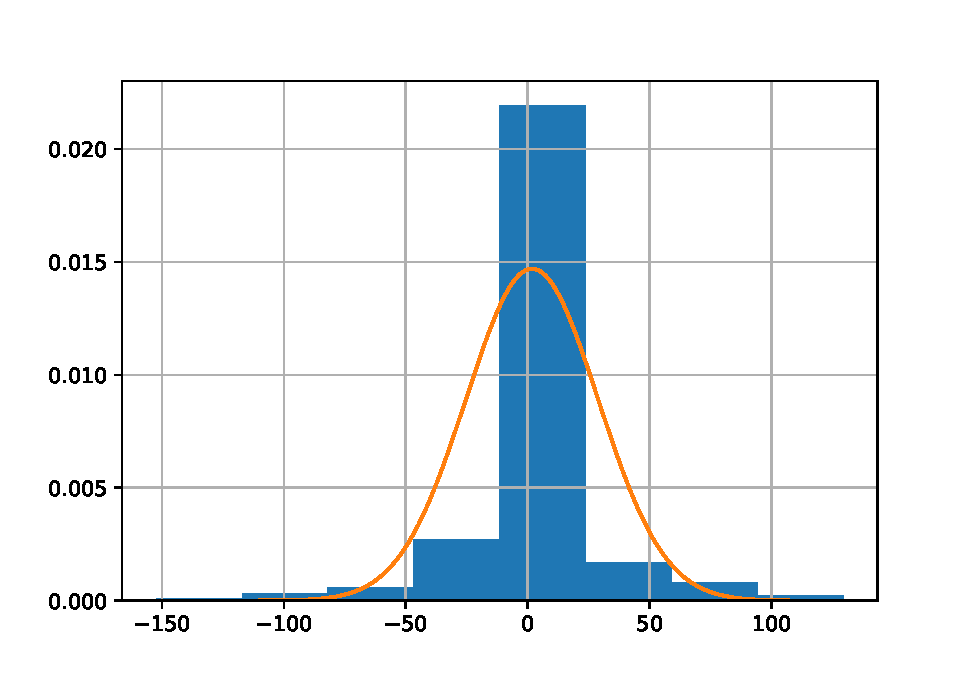
\includegraphics{_main_files/figure-latex/unnamed-chunk-170-1.pdf}

Egyszerűen \emph{utsukushii}, nemigaz? :) Szépen látszik, hogy a valódi árváltozás eloszlás kissé csúcsosabb, mint amit az adatokra illeszkedő normális eloszlás sűrűségfüggvénye sugall.

Egyébként majd ilyen elvi sűrűségfüggvények illeszkedési jóságát valós hisztogramokhoz egzaktabban is megtanuljuk majd mérni a félév során, mint a szemmelverés. :)

\subsection{Centrális Határeloszlás Tétel (CHT)}\label{centruxe1lis-hatuxe1reloszluxe1s-tuxe9tel-cht}

A normális eloszlás esetében viszont van egy \textbf{valószínűségszmítási tétel, ami megadja, hogy a normális eloszlás milyen tulajdonságú adatsorok esetén} lesz egy \textbf{jól illeszkedő eloszlás} a megfigyelt adatok hisztogramjára. Ez a tétel pedig a \textbf{Centrális Határeloszlás Tétel}, leánykori nevén \textbf{CHT}.
Maga a tétel azt mondja, hogy \textbf{ha az adatsor egy \(Y_i\) értéke véletlen hatások összegződéseként áll elő, akkor az adatok hisztogramja normális eloszlású sűrűségfüggvényt követ}.

A tétel tehát ilyen klasszikus \textbf{ha --\textgreater{} akkor} típusú matematiaki tétel. És az \textbf{``akkor'' utáni rész az érthetőbb}. Ha valami felétel teljesül, akkor az adatsorunk normális eloszlású. Ezt oké, értjük. De \textbf{mit jelent az a rész, ami a tétel feltételében van?} Hogy ha \textbf{az \(Y_i\) értékek véletlen hatások összegeként állnak elő}.

Nos, ez \textbf{utóbbi rész megértéséhez nézzünk rá ismét a Tesla árváltozások adatsorának első 5 elemére} a data frame \texttt{head} metódusával.

\begin{Shaded}
\begin{Highlighting}[]
\NormalTok{Tesla.head()}
\end{Highlighting}
\end{Shaded}

\begin{verbatim}
##        Dátum      TESLA
## 0 2019-05-07  -8.279998
## 1 2019-05-08  -2.220002
## 2 2019-05-09  -2.860000
## 3 2019-05-10  -2.459992
## 4 2019-05-13 -12.510009
\end{verbatim}

Vegyük például a 2019 május 13-i \(Y_5=-12.510009\$\)-os veszteséget. Nos \textbf{ez az érték úgy jött ki}, hogy \textbf{az adott nap} (2019. 05. 13.) \textbf{véletlenszerű gazdasági eseményeinek hatása összegződött}, és \textbf{így kötöttünk ki ott, hogy a Tesla részvény a nap végére kb. 12 és fél dollárral kevesebbet ér}. Tehát, reggel mondjuk bejelentik a kínaiak, hogy vizsgálatot indítanak az egyik Tesla gyár munkakörülményei ellen, aminek hatására elkezd esni a részvény értéke, de aztán délben Musk tweetel egyet, hogy ``no para, átviszem a gyárat Mexikóba'', aminek hatására nyugi lesz és elindul felfelé a részvény értéke, de aztán nap végére beesik egy hír, hogy a Mexikóban máris tümtikéznek a tervezett Tesla gyár ellen, ami megint elkezdi levinni a részvény értékét és a nap végére uda jutunk, hogy a részvény \(-12.510009\$\)-al zár\ldots{}
Szóval az \textbf{adott nap véletlenszerű gazdasági eseményeinek összegződéseként áll elő a nap végi \(Y_i\) Tesla árváltozás}. Ezt jelenti az, hogy \textbf{az \(Y_i\) értékek véletlen hatások összegeként állnak elő}. És \textbf{ilyen esetekben az \(Y_i\) adatsorhoz tartozó hisztogram normális eloszlású sűrűségfüggvényt követ a CHT szerint!}

Láthatjuk a \textbf{Tesla részvény vizsgálatának korábbi tapasztalataink alapján}, hogy a csúcsosság miatt azért \textbf{a pénzügyi piacokon ez a tétel nem érvényesül annyira pontosan}, de \textbf{közelítőleg} igen. De \textbf{több egyéb esetben elég szépen érvényesül}: Pl. egy termelőgép által a nap végén gyártott selejtes termékek száma esetén. Az adott napi selejtszám értéke (ha nincs szabotőr a gyárban) az adott napi véletlen hatások összegződése állítja elő. Így, ha több nap nap végi selejtszámait vizsgáljuk, akkor azok hisztogramja csudiszép normális eloszlást kell, hogy kirajzoljon.

\subsection{Inverz Értékek}\label{inverz-uxe9rtuxe9kek}

A sűrűségfüggvényektől lehet ``\emph{visszafelé is kérdezni}''. Tehát, nem csak arra képesek, hogy mondok egy eseményt (pl. mi a valószínűsége, hogy \(80\$\)-nál nagyobb veszteségem lesz a Teslán) és adnak hozzá valószínűséget, hanem arra is, hogy mondok nekik valószínűséget, és az \textbf{inverz értékeik} segítségével adnak hozzá értéket. Szóval, tudok tőlük olyat kérdezni, hogy pl. \emph{Mi az az érték, aminél csak \(5\%\) valószínűséggel veszítek többet a Teslán?}
Magyarul, a \(P(Y_i < x) = 0.05\) kifejezésben megadja nekem a sűrűségfüggvény inverz értéke az \(x\)-et. Ilyenkor az történik a háttérben, hogy a sűrűségfüggvény primitívfüggvényéből (amit hívnak eloszlásfüggvénynek is, de a mi szempontunkból ez az elnevezés nem fontos) ``\emph{kifejezzük az \(x\)-et}''.

Természetesen, a \texttt{scipy}-nak erre is van beépített függvénye \texttt{norm.ppf} néven, ami 3 paramétert kíván: a \(P(Y_i < x)\) alá esési valószínűséget (ezt a függvény \texttt{q}-nak hívja az angol kvantilis=quantile szóból), a \(\mu\) átlagot (\texttt{loc}) és a \(\sigma\) szórást (\texttt{scale}).
Akkor hát lássuk mi is az az érték, aminél csak \(5\%\) valószínűséggel veszítek többet a Teslán?

\begin{Shaded}
\begin{Highlighting}[]
\NormalTok{stats.norm.ppf(q }\OperatorTok{=} \FloatTok{0.05}\NormalTok{, loc }\OperatorTok{=}\NormalTok{ np.mean(Tesla.TESLA), scale }\OperatorTok{=}\NormalTok{ np.std(Tesla.TESLA))}
\end{Highlighting}
\end{Shaded}

\begin{verbatim}
## -42.85439941594264
\end{verbatim}

Oké, tehát csak \(5\%\) valószínűséggel veszítünk kb. \(42.85\$\)-nál többet. Vagy másképp: \(5\%\) a valószínűsége, hogy egy random napon a Tesla árváltozás kisebb lesz, mint \(-42.85\$\). Jó tudni. :) Amúgy pénzügyekben ezeket az értékeket \emph{5\%-os Value at Risk}-nek szokás becézni, mint 5\%-os kockáztatott érték. Általában úgy szól a törvényi szabályozás ezeket az értékeket a befektetési bankoknak be kell raknia biztonsági tartalékba egy-egy pénzügyi befektetési portfólió után.

Ha valaki mélyebben belegondol a Stat. I-es rémképeibe, az \textbf{eloszlások inverz értékeihez is találhat analógiát, mégpedig a percentiliseket!} Hiszen a megfigyelt árváltozások \textbf{5. percentilis}e megadja, hogy mi az az érték, aminél az adatok \(5\%\)-a kisebb csak. Tehát ez az értelmezés lehet a ``\emph{Mi az az érték, aminél csak \(5\%\) a valószínűsége, hogy egy random napon a Tesla árváltozás kisebb lesz?}'' c.~kérdés analógiája.

Lássuk, akkor mi a megfigyelt érváltozások 5. percentilise! Itt most a data frame \texttt{quantile} metódusát vetjük be, aminek a paraméterében tizedestörtként kell megadni a keresett percentilis sorszámát. Tehát az 5. percentilisnél \(0.05\)-öt adunk meg.

\begin{Shaded}
\begin{Highlighting}[]
\NormalTok{Tesla.TESLA.quantile(}\FloatTok{0.05}\NormalTok{)}
\end{Highlighting}
\end{Shaded}

\begin{verbatim}
## -28.48700139999998
\end{verbatim}

Ahha, ez csak kb. \(-28.5\$\)! Tehát a megfigyelt napjaink \(5\%\)-ban volt nagyobb veszteségünk, mint \(28.5\$\)! Ez azért \textbf{lényegesen kisebb érték, mint a sűrűségfüggvényből származó \(42.85\$\)-os veszteség!} És valószínűleg a \textbf{sűrűségfüggvény}ből származó éték a reálisabb, hiszen az a számolás során ugyebár \textbf{olyan értékeket is figyelembe vett} valami pozitív bekövetkezési valószínűséggel, \textbf{amiket a megfigyelt adatsor még egyáltalán ``nem is látott''}, mert kisebbek pl. mint a minimum értéke.
Tehát, megint elmondhatjuk, hogy \textbf{ha az elvi eloszlásból ``keresek percentilist'', akkor a megfigyelt adatokon kívüli világot is figyelembe veszem!} Azaz, \textbf{általánosítok}.

Az tehát, hogy mondjuk egy befektetési bank a befketetéseinek \emph{Value at Risk} értékét a megfigyelt korábbi adatokból, vagy egy azokra jól illeszkedő elvi eloszlásból számolja egyáltalán nem mindegy! Persze itt a jól illeszkedő eloszlás nem feltétlenül a normális eloszlás, de rengeteg egyéb, kellően egzotikus sűrűségfüggvénnyel rendelkező eloszlás van a palettán, lehet válogatni. :)
Persze a válogatáshoz dolgozni is kéne, és nagy a csábítás, hogy egyszerűen inkább a megfigyelt múltbeli adatok alapján mondjon az ember egy percentilist\ldots a nagy befektetési bankok többsége 2008 előtt ezt is csinálta, mert megtehette. Aztán a 2008-as pénzügyi válság lett belőle. Erről is szól részben a The Black Swan: The Impact of the Highly Improbable c.~könyv. Ajánlom minden érdeklődőnek, tartalmas és közérthető olvasmány. :)
2008 óta a törvényi szabályozás (Európában a Bázel III., 2023-tól Bázel IV.) kötelezi a bankokat, hogy a befektetéseikhez Value at Risk-et az adataikra megfelelően illeszkedő elvi eloszlásból számoljanak.

Természetesen ilyen inverz érték formájában ``pozitív'' dolgot is kérdezhetek: \textbf{Mi az az érték, aminél csak \(1\%\) a valószínűsége, hogy többet nyerünk egy Tesla részvényen?} Azaz, mi a \(99\%\)-os valószínűséggel elérhető legnagyobb nyereség?

Ekkor a kérdés ugyebár úgy szól matematikai formájában, hogy mi az az \(x\), aminél \(P(Y_i>x)=0.01\)-et kapunk. De mivel a \texttt{scipy} csomag \texttt{norm.ppf} függvénye \textbf{csak alá esési valószínűséghez tud visszakeresni értékeket}, így inkább a kérdés átfogalmazott verzióját kérdezzük meg a gépszellemtől: \textbf{Mi az az \(x\), aminél \(P(Y_i<x)=0.99\)-et kapunk?}

\begin{Shaded}
\begin{Highlighting}[]
\NormalTok{stats.norm.ppf(q }\OperatorTok{=} \FloatTok{0.99}\NormalTok{, loc }\OperatorTok{=}\NormalTok{ np.mean(Tesla.TESLA), scale }\OperatorTok{=}\NormalTok{ np.std(Tesla.TESLA))}
\end{Highlighting}
\end{Shaded}

\begin{verbatim}
## 64.91674710828752
\end{verbatim}

Tehát, csak \(1\%\) eséllyel tudok többet nyerni egy nap a Teslán, mint kb. \(65\$\).

\subsection{A Standard Normális Eloszlás}\label{a-standard-normuxe1lis-eloszluxe1s}

Még egy fontos dologról kell megemlékeznünk a normális eloszlás kapcsán, a \(\mu=0\) átlagú és \(\sigma=1\) szórású \(N(0,1)\) eloszlásról, ami \textbf{standard normális eloszlás} néven külön helyet kapott a pokolban.

Ami miatt külön kiemelt helye van ennek a standard normális eloszlásnak az az, hogy minden \(N(\mu,\sigma)\) normális eloszlás áttranszformálható strandard normális \(N(0,1)\) eloszlássá. Mégpedig a következő formulával. \[z_i=\frac{Y_i-\mu}{\sigma}\]

Tehát, ha egy \textbf{normális eloszlású \(Y_i\) adatsor minden eleméből kivonom az átlagot és az eredményt elosztom a szórással, akkor az így előálló \(z_i\) adatsor már standard normális eloszlású lesz}. Ez a művelet a \textbf{standardizálás/noralizálás művelet}e.

Amúgy azt, hogy egy adatsor/sokaság valamilyen eloszlást követ, azt \(\sim\) jellel szokás jelölni. Tehát azt mondhatom, hogy \(Y_i \sim N(\mu,\sigma)\), de \(z_i \sim N(0,1)\).

Lássuk is akkor a standardizálást a gyakorlatban a Tesla részvények árváltozásain, és állítsuk elő ezt a \(z_i\) oszlopot.

\begin{Shaded}
\begin{Highlighting}[]
\NormalTok{Tesla[}\StringTok{\textquotesingle{}z\_i\textquotesingle{}}\NormalTok{] }\OperatorTok{=}\NormalTok{ (Tesla.TESLA }\OperatorTok{{-}}\NormalTok{ np.mean(Tesla.TESLA))}\OperatorTok{/}\NormalTok{np.std(Tesla.TESLA)}
\BuiltInTok{round}\NormalTok{(Tesla.describe(), }\DecValTok{2}\NormalTok{) }\CommentTok{\# 2 tizedesre kereítés az átláthatóság miatt}
\end{Highlighting}
\end{Shaded}

\begin{verbatim}
##                             Dátum   TESLA     z_i
## count                         250  250.00  250.00
## mean   2019-11-02 15:56:09.600000    1.78    0.00
## min           2019-05-07 00:00:00 -152.36   -5.68
## 25%           2019-08-05 06:00:00   -3.77   -0.20
## 50%           2019-10-31 12:00:00    1.42   -0.01
## 75%           2020-02-02 06:00:00    6.96    0.19
## max           2020-05-01 00:00:00  129.43    4.70
## std                           NaN   27.19    1.00
\end{verbatim}

Láthatjuk a leíró statisztikákból, hogy a \(z_i\) adatsornak már kb. \(0\) az átlaga és kb. \(1\) a szórása 2 tizedesre kerekítve.

De a hisztogram alapján az eloszlás továbbra is normális maradt.

\begin{Shaded}
\begin{Highlighting}[]
\NormalTok{Tesla.z\_i.hist(bins}\OperatorTok{=}\DecValTok{8}\NormalTok{)}
\end{Highlighting}
\end{Shaded}

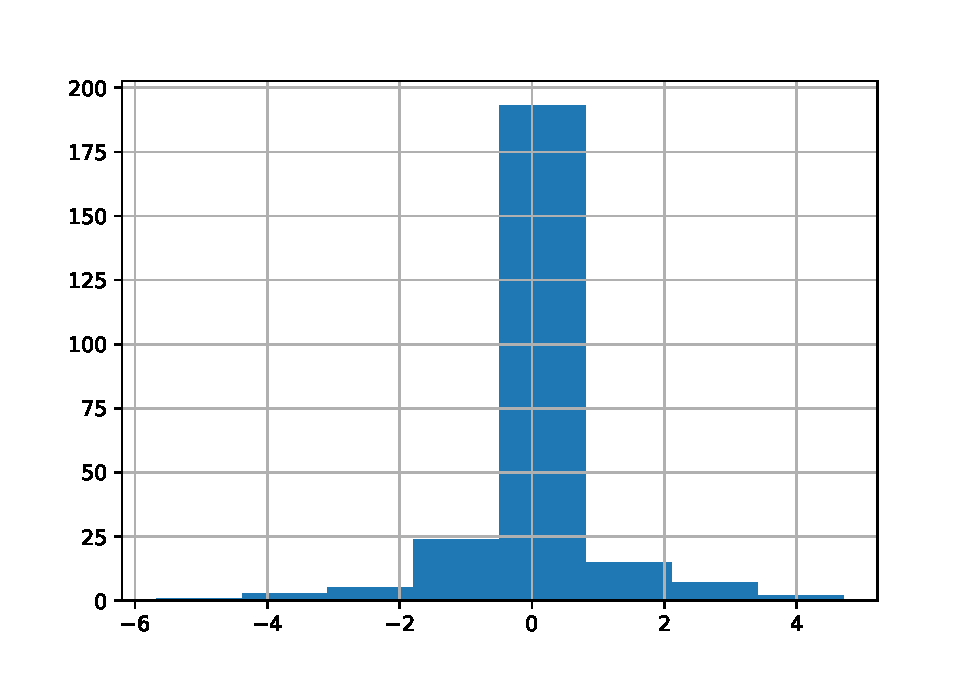
\includegraphics{_main_files/figure-latex/unnamed-chunk-176-3.pdf}

Ami miatt szeretni szokás a standard normális eloszlást az az a jellemzője, hogy

\begin{itemize}
\tightlist
\item
  Az adatok kb. középső \(68.2\%\)-a \(-1\) és \(+1\) között
\item
  Az adatok kb. középső \(95.4\%\)-a \(-2\) és \(+2\) között
\item
  Az adatok kb. középső \(99.7\%\)-a \(-3\) és \(+3\) között
\end{itemize}

helyezkedik el.

Ezt szemlélteti az alábbi ábra is.

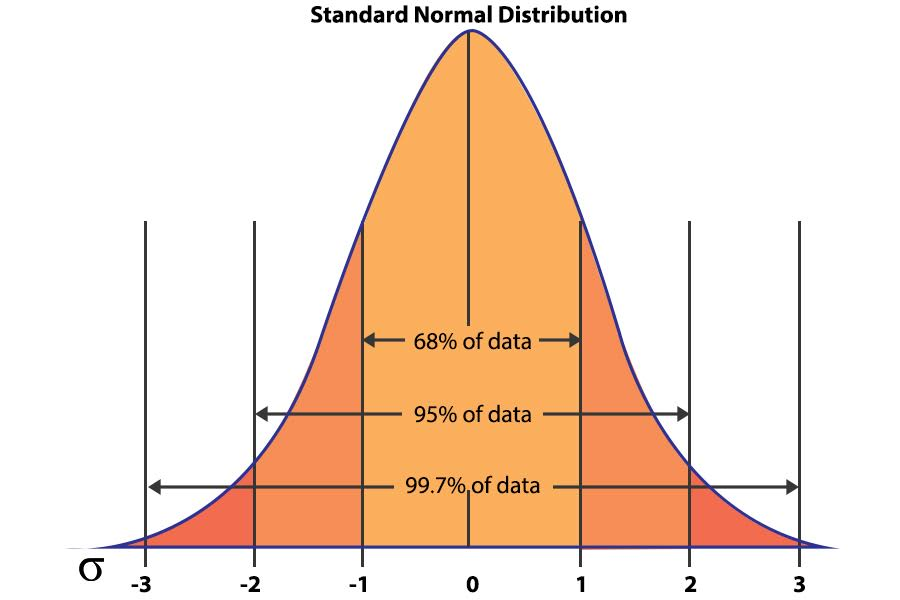
\includegraphics[width=0.5\textwidth,height=\textheight]{stnormal.png}

De ezt ellenőrizhetjük is könnyen Pythonban is, pl. a \(\pm2\)-re. A \texttt{norm.cdf} függvény ugyanis \texttt{loc=0} és \texttt{scale=1} beállításokkal fut, ha nem adunk meg neki mást. Tehát szűmoljuk ki \(z_i \sim N(0,1)\) esetén a \(P(-2 < z_i < +2)\) valószínűséget!

\begin{Shaded}
\begin{Highlighting}[]
\NormalTok{stats.norm.cdf(}\DecValTok{2}\NormalTok{)}\OperatorTok{{-}}\NormalTok{stats.norm.cdf(}\OperatorTok{{-}}\DecValTok{2}\NormalTok{)}
\end{Highlighting}
\end{Shaded}

\begin{verbatim}
## 0.9544997361036416
\end{verbatim}

Jé, ténlyeg kb. \(95.4\%\)! :) \textbf{Ezt a tulajdonságát majd ki fogjuk a későbbiekben használni a standard normális eloszlásnak, szóval jól jegyezzétek meg!} :)

A fenti tulajdonságok miatt sokan szokták úgy keresni a kilógó értékeket egy adatsorban, hogy standardizálják őket, és megnézik melyek azok az értékek, amik kívül esnek a \(\pm2\) intervallumon, mondván az ilyen értékek vagy az adatok alsó vagy a felső \(2.5\%\)-ba tartoznak (a sűrűségfüggvényből látszik, hogy a 95\%-on kívüli 5\% egyeneletesen oszlik meg a függvény két széla között\ldots szimmetriksu az eloszlás ugyebár :)).

Ezt az elvet mi is könnyen tudjuk alkalmazni:

\begin{Shaded}
\begin{Highlighting}[]
\NormalTok{Tesla[(Tesla.z\_i }\OperatorTok{\textless{}} \OperatorTok{{-}}\DecValTok{2}\NormalTok{) }\OperatorTok{|}\NormalTok{ (Tesla.z\_i }\OperatorTok{\textgreater{}} \DecValTok{2}\NormalTok{)]}
\end{Highlighting}
\end{Shaded}

\begin{verbatim}
##          Dátum       TESLA       z_i
## 185 2020-01-30   59.820008  2.138541
## 187 2020-02-03  129.429993  4.703562
## 188 2020-02-04  107.059998  3.879262
## 189 2020-02-05 -152.359986 -5.679967
## 197 2020-02-18   58.369995  2.085110
## 198 2020-02-19   59.019959  2.109060
## 201 2020-02-24  -67.210022 -2.542321
## 204 2020-02-27  -99.799988 -3.743211
## 206 2020-03-02   75.630005  2.721115
## 211 2020-03-09  -95.479980 -3.584026
## 214 2020-03-12  -73.679992 -2.780729
## 216 2020-03-16 -101.549988 -3.807696
## 218 2020-03-18  -68.980011 -2.607542
## 219 2020-03-19   66.420014  2.381741
## 222 2020-03-24   70.709991  2.539820
## 235 2020-04-13   77.950012  2.806604
## 236 2020-04-14   58.940003  2.106114
## 241 2020-04-21  -59.640014 -2.263378
## 245 2020-04-27   73.599976  2.646312
## 249 2020-05-01  -80.559998 -3.034247
\end{verbatim}

Meg is vannak a kiugróan nagy veszteséget vagy nyereséget szolgáltató napjaink. :)

De \textbf{ezzel a módszerrel vigyázzunk!} A standardizált \(z_i\) értékek alapján történő kilógó érték keresés \textbf{csak akkor működik, ha az eredeti (standardizálás előtti) adatsorunk is már eleve normális eloszlású volt!} Hiszen csak ekkor lesz a transzformált adatsor is szimmetrikus normális eloszlású és lesz igaz rá a \(P(-2 < z_i < +2)=0.954\) összefüggés!
Szóval \textbf{kilógó érték kereséshez inkább használjuk} a tetszőleges eloszlásokon is működőképes \textbf{doboz ábrás módszert}! :)

Még egy utolsó gondolat. A standardizált \(z_i\) értékeknek van egy olyan értelmezése is, hogy megadják, az adott érték a \(\sigma\) szórás hányszorosával tér el a \(\mu\) átlagtól.
Tehát, pl. a fenti szűrésben szereplő 2020 január 30-i \(59.82\$\)-os árváltozás a \(27.19\)-es szórás kb. \(2.14\)-szeresével tér el az \(1.8\$\)-os átlagtól.

\section{Az Exponenciális eloszlás}\label{az-exponenciuxe1lis-eloszluxe1s}

Na, hát akkor most engedjük el egy kicsit a Tesla részvények árváltozásait, és vizsgáljunk meg egy másik adatsort, ami a CancerSurvival.xlsx fájlban lakik. Ebben az adattáblában 58 súlyos fej- és nyakrák páciensről rögzítették, hogy \emph{hány hónapig} maradtak életben kemoterápia után. Az adatok valósak, 1988-ból a forrás ez a tanulmány.

Töltsük is be az adatokat egy \texttt{pandas} data frame-be!

\begin{Shaded}
\begin{Highlighting}[]
\NormalTok{Surv }\OperatorTok{=}\NormalTok{ pd.read\_excel(}\StringTok{"CancerSurvival.xlsx"}\NormalTok{)}

\NormalTok{Surv.info()}
\end{Highlighting}
\end{Shaded}

\begin{verbatim}
## <class 'pandas.core.frame.DataFrame'>
## RangeIndex: 58 entries, 0 to 57
## Data columns (total 2 columns):
##  #   Column     Non-Null Count  Dtype  
## ---  ------     --------------  -----  
##  0   Sorszám    58 non-null     float64
##  1   SurvMonth  58 non-null     float64
## dtypes: float64(2)
## memory usage: 1.0 KB
\end{verbatim}

\begin{Shaded}
\begin{Highlighting}[]
\NormalTok{Surv.head()}
\end{Highlighting}
\end{Shaded}

\begin{verbatim}
##    Sorszám  SurvMonth
## 0      1.0       6.53
## 1      2.0       7.00
## 2      3.0      10.42
## 3      4.0      14.48
## 4      5.0      16.10
\end{verbatim}

Mint láthatjuk, ebben a data frame-ben is csak két oszlopunk van. Az első a páciens sorszáma, a második pedig a kemoterápiától számítot túlélési idő hónapokban megadva (\emph{SurvMonth}).

Nézzünk rá egy hisztogrammal a túlélési idők eloszlására. Mivel most \(N=58\), így a legksiebb olyan \(k\), amire \(2^k\) már épp nagyobb \(N\)-nél az a 6 lesz, hiszen \(2^6=64\). Tehát \(6\) osztályközt hozunk létre a hisztogramon.

\begin{Shaded}
\begin{Highlighting}[]
\NormalTok{Surv.SurvMonth.hist(bins}\OperatorTok{=}\DecValTok{6}\NormalTok{)}
\end{Highlighting}
\end{Shaded}

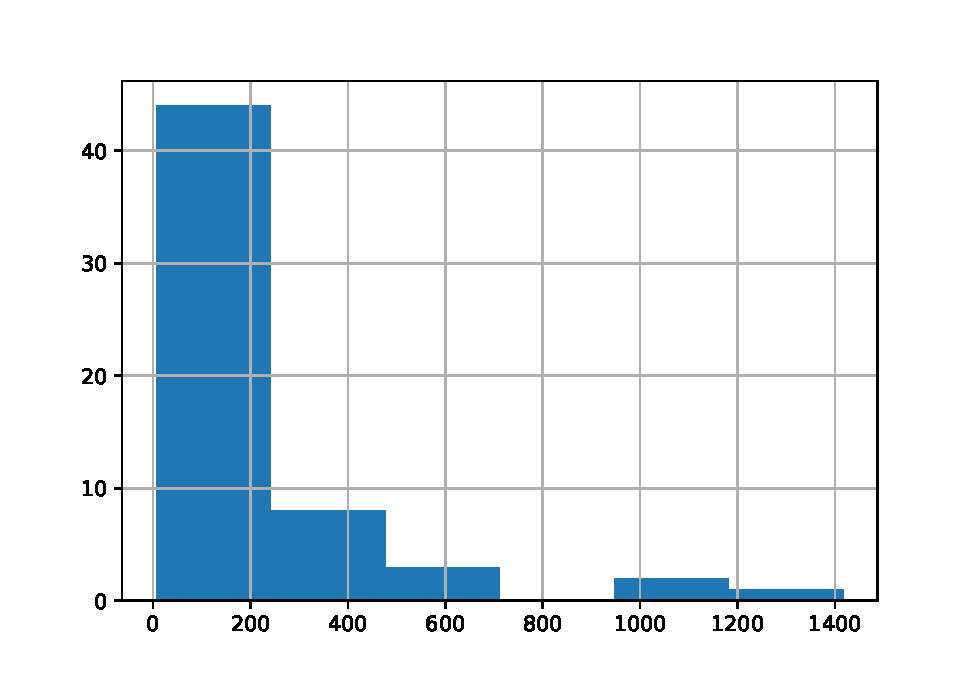
\includegraphics{_main_files/figure-latex/unnamed-chunk-180-5.pdf}

Nos, hát itt az látszódik, hogy az eloszlásunk jobbra elnyúló: a túlélési idők nagy többsége (45 az 58-ból konkrétan) \(256\) hónapon belüli, de a maradék \(13\) meghaladja ezt, sőt \(3\) páciens \(1000\) hónapnál is hosszabb ideig élt túl a kemoterápia után.

A jobbra elnyúlás miatt, ha folytonos vonallal összekötjük a hisztogram oszlopait, akkor valami ilyesmi függvényábrát kapunk, mint alább.

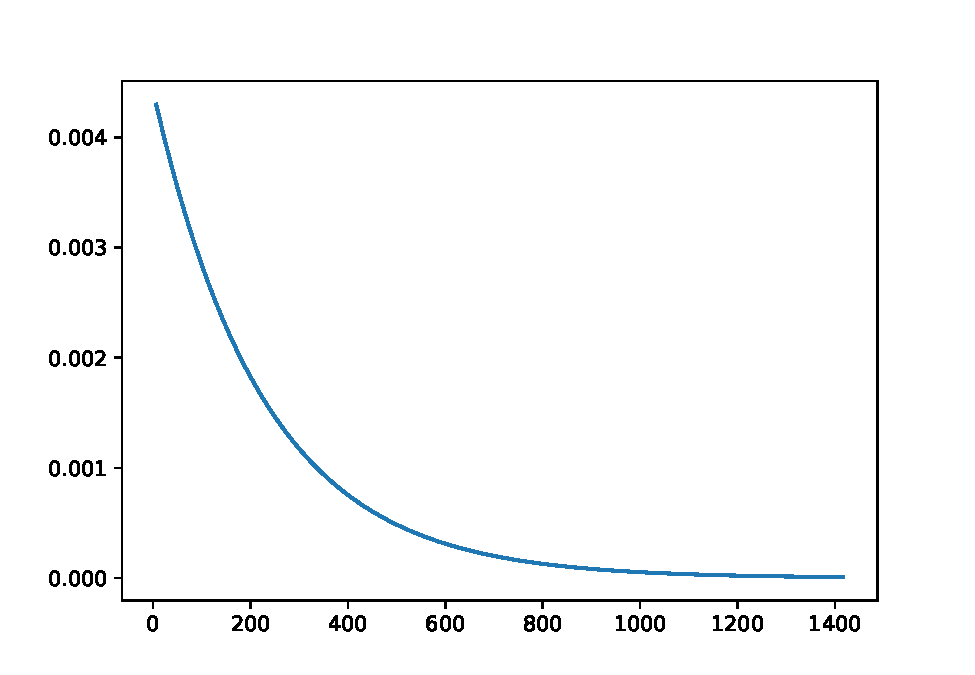
\includegraphics{_main_files/figure-latex/unnamed-chunk-181-7.pdf}

Ez az alakzat pedig az \textbf{exponenciális eloszlás sűrűségfüggvénye}. Ennek a sűrűségfüggvénynek a konkrét alakját egy \(\lambda\) paraméter határozza meg. Minél nagyobb \(\lambda\), annál meredekebben jobbra elnyúló a sűrűségfüggvény. Ezt alább lehet kipróbálni.

Természetesen a \(\lambda\)-nak van köze a valós adatok átlagához és szórásához, egész konkrétan mindkét érték \(\mu=\sigma=\frac{1}{\lambda}\). Tehát, az exponenciális eloszlásban azonos átlagot és szórást tételezünk fel az adatokra, és ennek a közös értéknek a reciproka (a \(\lambda\)) határozza meg, hogy mennyire meredeken nyúlik jobbra az eloszlás sűrűségfüggvénye. Emiatt az exponenciális eloszlásokat \(Exp(\lambda)\) módon szokták jelölni.

Persze valós adatokon gyakorlatilag sosem fog teljesülni, hogy \(\mu=\sigma\), de láthatjuk egy \texttt{describe} metódusból, hogy a túlélési adatok esetén a két mutató értéke aránylag közel esik egymáshoz: \(\mu=226.17 \approx \sigma=273.94\)

\begin{verbatim}
## count      58.000000
## mean      226.173793
## std       273.943381
## min         6.530000
## 25%        83.250000
## 50%       151.500000
## 75%       237.000000
## max      1417.000000
## Name: SurvMonth, dtype: float64
\end{verbatim}

A \texttt{scipy} csomagban a \texttt{norm.pdf}, \texttt{norm.cdf} és \texttt{norm.ppf} függvények mintájára léteznek \texttt{expon.pdf}, \texttt{expon.cdf} és \texttt{expon.ppf} függvények is. Használatuk és jelentésük teljesen megegyezik a normális eloszlásnál látott függvényekkel. Egyetlen különbség ugyebár, hogy exponenciális eloszlásnál csak az egységes \(\lambda\)-t kell megadni a külön \(\mu\) és \(\sigma\) helyett, mint ahogy a normális eloszlásnál működött a dolog.
A \texttt{scipy} csomag ezt úgy oldja meg, hogya a szórásból számolja vissza a \(\lambda\)-t, tehát a függvényeknek a \texttt{scale} paraméterében kell átadni az adatok szórását, amire az exponenciális eloszlást illeszteni akarjuk.
Ez alapján akkor most a túlélési idők esetében \(\lambda=\frac{1}{\sigma}=\frac{1}{273.94}=0.00365\). Tehát az egyes \(Y_i\) túlélési idők \(Exp(0.00365)\) eloszlástkövetnek: \(Y_i \sim Exp(0.00365)\)

Ezek alapján számoljunk ki pár valószínűséget a túlélési időkre vonatkozóan:

\begin{enumerate}
\def\labelenumi{\arabic{enumi}.}
\tightlist
\item
  Mi a valószínűsége, hogy kemoterápia után pont egy évet, azaz \(12\) hónapot fogunk élni?
\end{enumerate}

\begin{Shaded}
\begin{Highlighting}[]
\NormalTok{stats.expon.pdf(}\DecValTok{12}\NormalTok{, scale }\OperatorTok{=}\NormalTok{ np.std(Surv.SurvMonth))}
\end{Highlighting}
\end{Shaded}

\begin{verbatim}
## 0.003523104116060953
\end{verbatim}

Ez egy jó alacsony, kb. \(0.3\%\)-os valószínűség. Nem lepődünk meg, hiszen egy konkrét pont bekövetkezése a nagy túlélési idő-értékkészlet miatt itt is kicsi.

\begin{enumerate}
\def\labelenumi{\arabic{enumi}.}
\setcounter{enumi}{1}
\tightlist
\item
  Mi a valószínűsége, hogy kemoterápia után több, mint öt évet, azaz \(60\) hónapot fogunk élni?
\end{enumerate}

\begin{Shaded}
\begin{Highlighting}[]
\DecValTok{1} \OperatorTok{{-}}\NormalTok{ stats.expon.cdf(}\DecValTok{60}\NormalTok{, scale }\OperatorTok{=}\NormalTok{ np.std(Surv.SurvMonth))}
\end{Highlighting}
\end{Shaded}

\begin{verbatim}
## 0.8017677791228195
\end{verbatim}

Az eredmény kb. \(80\%\), egész jó kilátások!

\begin{enumerate}
\def\labelenumi{\arabic{enumi}.}
\setcounter{enumi}{2}
\tightlist
\item
  Mi a valószínűsége, hogy a kemoterápia utáni harmadik év során, azaz \(24\) és \(36\) hónapközött fogunk elpatkolni?
\end{enumerate}

\begin{Shaded}
\begin{Highlighting}[]
\NormalTok{stats.expon.cdf(}\DecValTok{36}\NormalTok{, scale }\OperatorTok{=}\NormalTok{ np.std(Surv.SurvMonth)) }\OperatorTok{{-}}\NormalTok{ stats.expon.cdf(}\DecValTok{24}\NormalTok{, scale }\OperatorTok{=}\NormalTok{ np.std(Surv.SurvMonth))}
\end{Highlighting}
\end{Shaded}

\begin{verbatim}
## 0.03956914214644276
\end{verbatim}

A számítások alapja itt is az, hogy \(f(x)=P(Y_i=x)\), tehát \textbf{a sűrűségfüggvény helyettesítési értékre \(x\) helyen megegyezik az \(x\) érték bekövetkezési valószínűségével} egy véletlen húzás esetén az adatsorból. A \(P(Y_i<x)\) valószínűség pedig exponenciális sűrűségfüggvény esetén is az \(\int_{-\infty}^x{f(x)}dx\) improprius integrállal számítható, azaz a sűrűségfüggvény \(x\) alatti területével egyezik meg.

Ezeket a vizuális jelentéstartalmakat az alábbi interaktív ábrán meg lehet nézni és ki lehet próbálni úgy, ahogy a normális eloszlásnál lehetett.

Természetesen \emph{inverz értéket} is tudunk számolni az exponenciális eloszlásban is. Nézzük meg pl, hogy Mi az az idő, aminél csak \(1\%\) a valószínűsége, hogy egy kemoterápiával kezelt fej- és nyakrák páciens tovább él.
Ugyebár a számításhoz úgy kell átfogalmazni a kérdést, hogy mi az az idő, ami esetén csak \(99\%\) a valószínűsége, hogy egy kemoterápiával kezelt fej- és nyakrák páciens már \emph{NEM} él tovább. Hiszen az \texttt{expon.ppf} függvény is \emph{alá esési} valószínűségekból dolgozik, mint a \texttt{norm.ppf}.

\begin{Shaded}
\begin{Highlighting}[]
\NormalTok{stats.expon.ppf(}\FloatTok{0.99}\NormalTok{, scale }\OperatorTok{=}\NormalTok{ np.std(Surv.SurvMonth))}
\end{Highlighting}
\end{Shaded}

\begin{verbatim}
## 1250.6331218835987
\end{verbatim}

A megfejtés kb. \(1250\) hónap, azaz \(104\) év! De hát ugye ez a nagy érték alapvetően a jobbra elnyúlás miatt van, hiszen a jobbra elnyúló eloszlásokra jellemzőek a felfelé kilógó értékek, így a jobbra elnyúló sűrűségfüggvényeknek is számolnia kell ezekkel az outlier elemekkel.

Végül pedig nézzük meg szépen, hogy ez az exponenciális sűrűségfüggvény mennyire illeszkedik a túlélési idők hisztogramjára, ahogy a normális eloszlás esetén is megtettük egy hisztogramra illesztett \texttt{matplotlib}-es vonaldiagrammal.

\begin{Shaded}
\begin{Highlighting}[]
\NormalTok{Surv.SurvMonth.hist(bins }\OperatorTok{=} \DecValTok{6}\NormalTok{, density }\OperatorTok{=} \VariableTok{True}\NormalTok{)}
\NormalTok{x\_tengely }\OperatorTok{=}\NormalTok{ np.arange(np.}\BuiltInTok{min}\NormalTok{(Surv.SurvMonth), np.}\BuiltInTok{max}\NormalTok{(Surv.SurvMonth), }\FloatTok{0.01}\NormalTok{)}
\NormalTok{y\_tengely }\OperatorTok{=}\NormalTok{ stats.expon.pdf(x\_tengely, scale }\OperatorTok{=}\NormalTok{ np.mean(Surv.SurvMonth))}
\NormalTok{plt.plot(x\_tengely, y\_tengely)}
\NormalTok{plt.show()}
\end{Highlighting}
\end{Shaded}

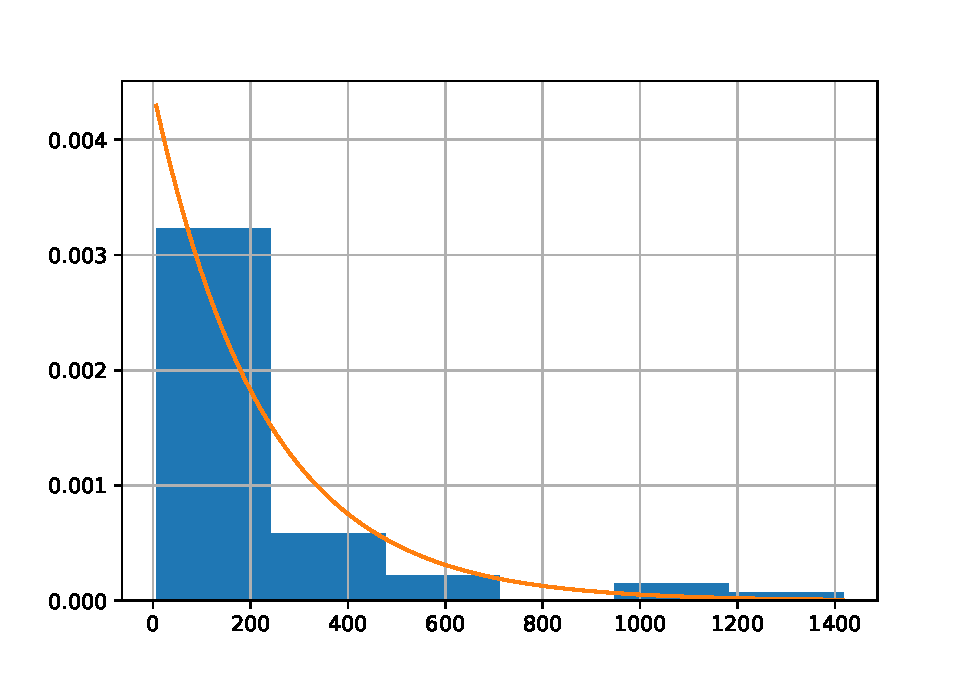
\includegraphics{_main_files/figure-latex/unnamed-chunk-189-1.pdf}

Itt egész pofásnak tűnik az illeszkedés, így szemmelverésre jobban is illeszkedik ez az exponenciális eloszlás a túlélési időkre, mint a normális eloszlás illeszkedett a Tesla árváltozásokra. :)

\section{A Varianciahányados Pythonban - Kokain a Balatonban}\label{a-varianciahuxe1nyados-pythonban---kokain-a-balatonban}

Egy dolgot kellene még átismételnünk a Stat. I-es rémképeink közül, ami többször is elő fog jönni a Stat. II-es tanulmányinkban: a \textbf{Varianciahányados} fogalmát.

A varianciahányados ugyebár arra szolgál, hogy \textbf{két ismérv, egy minőségi (``szöveges'') és egy mennyiségi (``számértékű'') ismérv kapcsolatának szorosságát adja meg, százalékos formában}. Tehát olyan kérdéseket lehet vele megválaszolni, mint\ldots{}

\begin{itemize}
\tightlist
\item
  Hány százalékban befolyásolja a nem (minőségi simérv) a fizetést (mennyiségi ismérv)?
\item
  Hány százalékban befolyásolja a kerület (minőségi simérv) a budapesti lakások árát (mennyiségi ismérv)?
\item
  Hány százalékban befolyásolja a Balaton Sound jelenléte (minőségi simérv) a Balatonban található kokain mennyiségét (mennyiségi ismérv)?
\end{itemize}

A legutolsó kérdés a listán elsőre meredeknek tűnik, de ez a tanulmány épp egy ilyen kérdésekkel is foglalkozik. Az általuk használt adatok egy részét találjuk a BalatonSoundCocaine.xlsx című fájlban.

A fájlban \textbf{3 balatoni vízminőséget ellenőrző állomás összesen \(N=540\) mérését látjuk}. Egy állomás egy hónapban \(20\) mérést végez, és mindhárom állomás esetén a nyári hónapok (június, július, augusztus) mérései vannak a fájlban 3 évre (2017, 2018, 2019). Így egy állomás esetében \(20 \times 3 \times 3 = 180\) mérésünk van, azaz a három állomásra összesen \(3 \times 180 = 540\) mérési adatunk van. Az \textbf{Excel fájlunk mindegyik mérés esetében tartalmazza a mérőállomás sorszámát (1., 2., 3.), a mérés évét és hónappját, valamint a vízben mért kokain mennyiségét nanogram/literben}.

Olvassuk is be az Excelt egy data frame-be és lessük meg, hogy ez tényleg így van-e!

\begin{Shaded}
\begin{Highlighting}[]
\NormalTok{Balcsi }\OperatorTok{=}\NormalTok{ pd.read\_excel(}\StringTok{"BalatonSoundCocaine.xlsx"}\NormalTok{)}

\NormalTok{Balcsi.info()}
\end{Highlighting}
\end{Shaded}

\begin{verbatim}
## <class 'pandas.core.frame.DataFrame'>
## RangeIndex: 540 entries, 0 to 539
## Data columns (total 4 columns):
##  #   Column   Non-Null Count  Dtype  
## ---  ------   --------------  -----  
##  0   Ev       540 non-null    int64  
##  1   Honap    540 non-null    object 
##  2   Allomas  540 non-null    object 
##  3   Kokain   540 non-null    float64
## dtypes: float64(1), int64(1), object(2)
## memory usage: 17.0+ KB
\end{verbatim}

\begin{Shaded}
\begin{Highlighting}[]
\NormalTok{Balcsi.head()}
\end{Highlighting}
\end{Shaded}

\begin{verbatim}
##      Ev   Honap     Allomas   Kokain
## 0  2017  június  1. állomás  0.03891
## 1  2017  június  1. állomás  0.01879
## 2  2017  június  1. állomás  0.03193
## 3  2017  június  1. állomás  0.03510
## 4  2017  június  1. állomás  0.01107
\end{verbatim}

Igen, az oszlopok (ismérvek) neve és adattípusa és az első öt sor tartalma alapján úgy néz ki, hogy rendben van a tábla, azok az oszlopok szerepelnek benne, amit a leírás alapján vártunk is.

Oké, akkor itt mérési adatokat látunk. Hogy a túróba jön az egészhez a Balaton Sound. Egyrészt úgy, hogy a három mérőállomás épp a Sound helyszíne környékén található Siófokon. Konkrét koordináták az alábbi ábrán.

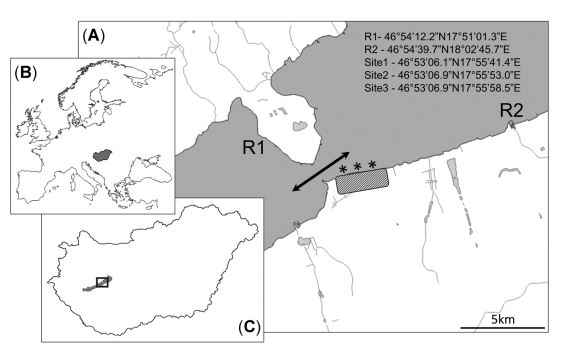
\includegraphics[width=0.5\textwidth,height=\textheight]{balcsi.jpg}

És hát a mérések pont a fesztivál előtt (június), közben (július) és után (augusztus) készültek. Tehát, ha \textbf{a Sound jelenlétének van hatása a víz kokain tartalmára, akkor a mérés hónapja aránylag nagy százalékban kell, hogy meghatározza a kokaintartalmat}. Szóval a vizsgált \textbf{minőségi ismérvünk a mérés hónapja, mennyiségi ismérvünk a kokaintartalom} lesz. A két ismérv kapcsolatának szorosságát pedig akkor a varianciahányados adja meg.

A varianciahányados kiszámításának első lépése egy olyan segétáblázat összeállítása, amely sorait a minőségi ismérv lehetséges értékei adják, és 3 oszlopa van, ami a minőségi ismérv \(j\) indexszel jelölt csoportjai szerint bontva tartalmazza az elemszámokat (\(N_j\)), a mennyiségi ismérv részátlagait (\(\bar{Y}_j\)) és szórásait (\(\sigma_j\)).
Ezt a segédtáblát Pythonban a data frame-k \texttt{groupby} és \texttt{agg} metódusaival hozhatjuk létre. Persze az \texttt{agg}-n belül használjuk a \texttt{numpy} csomag \texttt{mean} és \texttt{std} függvényeit is a \texttt{count} mellett (amely utóbbi függvényt stringként kell beadni az \texttt{agg}-ba, mint az oszlopneveket). Illetve, ne felejtsük el a végén a `reset\_index`` metódus használatát, különben a minőségi ismérvünk értékei a data frame sorindexeiként végzik, és nem lesz külön oszlopuk!

\begin{Shaded}
\begin{Highlighting}[]
\NormalTok{Segéd }\OperatorTok{=}\NormalTok{ Balcsi.groupby(}\StringTok{\textquotesingle{}Honap\textquotesingle{}}\NormalTok{).agg(}
\NormalTok{  Elemszam }\OperatorTok{=}\NormalTok{ (}\StringTok{\textquotesingle{}Kokain\textquotesingle{}}\NormalTok{, }\StringTok{\textquotesingle{}count\textquotesingle{}}\NormalTok{),}
\NormalTok{  Reszatlagok }\OperatorTok{=}\NormalTok{ (}\StringTok{\textquotesingle{}Kokain\textquotesingle{}}\NormalTok{, np.mean),}
\NormalTok{  Szorasok }\OperatorTok{=}\NormalTok{ (}\StringTok{\textquotesingle{}Kokain\textquotesingle{}}\NormalTok{, np.std)}
\NormalTok{).reset\_index()}
\end{Highlighting}
\end{Shaded}

\begin{verbatim}
## <string>:1: FutureWarning: The provided callable <function mean at 0x000001CA046C13A0> is currently using SeriesGroupBy.mean. In a future version of pandas, the provided callable will be used directly. To keep current behavior pass the string "mean" instead.
## <string>:1: FutureWarning: The provided callable <function std at 0x000001CA046C14E0> is currently using SeriesGroupBy.std. In a future version of pandas, the provided callable will be used directly. To keep current behavior pass the string "std" instead.
\end{verbatim}

\begin{Shaded}
\begin{Highlighting}[]
\NormalTok{Segéd}
\end{Highlighting}
\end{Shaded}

\begin{verbatim}
##        Honap  Elemszam  Reszatlagok   Szorasok
## 0  augusztus       180     0.029198   0.011618
## 1     július       180    64.859463  95.853905
## 2     június       180     0.029752   0.011614
\end{verbatim}

Meg is vagyunk! Látszik, hogy \textbf{a Sound hónapjának van hatása}: júliusban nagyságrendekkel több az átlagos kokain mennyisége a Balaton vizének, mint a másik két nyári hónapban. De a \textbf{hatás nagyságát nehéz megfogni már szemmelveréssel}, mivel a \textbf{kokain mennyiségek szórása is ebben a hónapban a legnagyobb}. Sőt, ez az egyetlen hónap, amikor a konkrét mérések kokain mennyiségének szórása \emph{nagyobb} az átlagos kokain mennyiségnél! Szóval, kell azért egy check arra a varianciahányadosra.

A varianciahányados, a \(H^2\) mutató értékéhez úgy jutunk el, hogy \textbf{elkezdjük az előbb felépített segédtáblázatunk alapján kiszámolni a mennyiségi ismérv (azaz most a kokain mennyiség) teljes, hónapoktól független teljes átlagát és teljes szórását}. Ugyebár a \textbf{teljes átlagos kokainmennyiség (főátlag, \(\bar{Y}\)), nem más, mint a részátlagok (\(\bar{Y}_j\)) részelemszámokkal (\(N_j\)) súlyozott átlaga}: \[\bar{Y}=\frac{\sum_j{N_j\bar{Y}_j}}{\sum_j{N_j}}\]

Ilyen stílusú súlyozott átlagokat számolgattunk már az 1.4. fejezetben, csak gyakorisági táblából. Ez ugyan az a szitu, és itt is a \texttt{np.sum} függvényt be tudjuk vetni. Ellenőrzéshez ki tudjuk számolni ezt a főátlagot úgy is, hogy az \texttt{np.mean} függvényt ráeresztjük a data frame teljes \texttt{Kokain} oszlopára.

\begin{Shaded}
\begin{Highlighting}[]
\NormalTok{főátlag }\OperatorTok{=}\NormalTok{ np.}\BuiltInTok{sum}\NormalTok{(Segéd.Elemszam }\OperatorTok{*}\NormalTok{ Segéd.Reszatlagok)}\OperatorTok{/}\NormalTok{(np.}\BuiltInTok{sum}\NormalTok{(Segéd.Elemszam))}
\NormalTok{főátlag}
\end{Highlighting}
\end{Shaded}

\begin{verbatim}
## 21.63947090740741
\end{verbatim}

\begin{Shaded}
\begin{Highlighting}[]
\NormalTok{np.mean(Balcsi.Kokain)}
\end{Highlighting}
\end{Shaded}

\begin{verbatim}
## 21.639470907407407
\end{verbatim}

Stimm egészen az utolsó jó sokadik tizedesjegyig. Ezzel megvagyunk. :)

A variancia-hányados lelke viszont abban leledzik, hogy a kokainmennyiség (mint mennyiségi ismérv) teljes szórása (\(\sigma\)) csak úgy kapható meg a segédtábla alapján, ha előbb kiszámoljuk a belső szórást (\(\sigma_B\)) és a külső szórást (\(\sigma_K\)).

A belső szórást a \textbf{belső variancián, azaz belső szórásnégyzeten keresztül kapjuk meg}. Ez pedig nem más, mint a \textbf{részszórások \(\sigma_j^2\) négyzeteinek elemszámokkal (\(N_j\)) súlyozott átlaga}. \[\sigma_B^2=\frac{\sum_j{N_j\sigma_j^2}}{\sum_j{N_j}}\]

Az előző számítás alapján ez is egész könnyen tud menni Pythonban, csak a részszórások négyzetre emelésére kell figyelni.

\begin{Shaded}
\begin{Highlighting}[]
\NormalTok{belső\_var }\OperatorTok{=}\NormalTok{ np.}\BuiltInTok{sum}\NormalTok{(Segéd.Elemszam }\OperatorTok{*}\NormalTok{ Segéd.Szorasok}\OperatorTok{**}\DecValTok{2}\NormalTok{)}\OperatorTok{/}\NormalTok{(np.}\BuiltInTok{sum}\NormalTok{(Segéd.Elemszam))}
\NormalTok{belső\_var}
\end{Highlighting}
\end{Shaded}

\begin{verbatim}
## 3062.6571029636407
\end{verbatim}

A belső szórás pedig egyszerűen a belső variancia gyöke. \(\sigma_B=\sqrt{\sigma_B^2}\) Általánosságban \(\sigma_B\) azt jelenti, hogy \textbf{egy véletlenszerűen kiválasztott egyed konkrét mennyiségi ismérv értéke várhatóan mennyivel tér el saját csoportjának átlagától}.

Konkrét esetünkben ez az alábbi módon néz ki.

\begin{Shaded}
\begin{Highlighting}[]
\NormalTok{belső\_szórás }\OperatorTok{=}\NormalTok{ np.sqrt(belső\_var)}
\NormalTok{belső\_szórás}
\end{Highlighting}
\end{Shaded}

\begin{verbatim}
## 55.34127847243539
\end{verbatim}

Tehát, \textbf{egy mérés kokainmennyisége várhatóan \(55.3\) nanogram/literrel tér el saját hónapjának átlagos kokainmennyiségtől}. Ami azért nem egy elhanyagolható mennyiségű szóródás a mérési hónapokon \emph{belül}.

A másik vége a dolognak a külső szórás, ami szintén a négyzetén, a külső variancián keresztül számítható. A külső variancia pedig a \textbf{részátlagok \(\bar{Y}_j\) elemszámokkal (\(N_j\)) súlyozott szórása a mennyiségi ismérv főátlaga \(\bar{Y}\) körül}. \[\sigma_K^2=\frac{\sum_j{N_j(\bar{Y}_j-\bar{Y})^2}}{\sum_j{N_j}}\]

Az 1.4. fejezet alapján ezt is meg tudjuk azért alkotni \texttt{np.sum} bevetésével.

\begin{Shaded}
\begin{Highlighting}[]
\NormalTok{külső\_var }\OperatorTok{=}\NormalTok{ np.}\BuiltInTok{sum}\NormalTok{(Segéd.Elemszam }\OperatorTok{*}\NormalTok{ (Segéd.Reszatlagok }\OperatorTok{{-}}\NormalTok{ főátlag)}\OperatorTok{**}\DecValTok{2}\NormalTok{)}\OperatorTok{/}\NormalTok{(np.}\BuiltInTok{sum}\NormalTok{(Segéd.Elemszam))}
\NormalTok{külső\_var}
\end{Highlighting}
\end{Shaded}

\begin{verbatim}
## 933.983870298589
\end{verbatim}

A külső szórás pedig egyszerűen a külső variancia gyöke. \(\sigma_K=\sqrt{\sigma_K^2}\) Általánosságban \(\sigma_K\) azt jelenti, hogy \textbf{egy csoport átlaga várhatóan mennyivel tér el a mennyiségi ismérv főátlagától}.

Konkrét esetünkben ez az alábbi módon néz ki.

\begin{Shaded}
\begin{Highlighting}[]
\NormalTok{külső\_szórás }\OperatorTok{=}\NormalTok{ np.sqrt(külső\_var)}
\NormalTok{külső\_szórás}
\end{Highlighting}
\end{Shaded}

\begin{verbatim}
## 30.561149688756622
\end{verbatim}

Tehát, \textbf{egy hónap átlagos kokainmennyisége várhatóan \(30.5\) nanogram/literrel tér el az átlagosan mért kokainmennyiségétől}. Tehát a hónapok \emph{között} is van egy jelentős szóródásunk, viszont ez kicsit kisebb, mint a csoporton belüli szóródás.

Ebből a két tényezőből pedig összeadható a \textbf{teljes variancia: \(\sigma^2=\sigma_B^2+\sigma_K^2\).} A teljes szórás pedig ennek a mennyiségnek a gyöke: \(\sigma=\sqrt{\sigma^2}=\sqrt{\sigma_B^2+\sigma_K^2}\). \textbf{Mivel tagonként nem vonhatunk gyököt, így ez az összefüggés ugyebár a szórásokra NEM lesz igaz!!}

A teljes szórás pedig \textbf{általánosan ugye azt mutatja meg, hogy egy véletlenszerűen kiválasztott egyed konkrét mennyiségi ismérv értéke várhatóan mennyivel tér el a mennyiségi ismérv csoportoktól független, teljes főátlagától}.

Lássuk, hogy ez a mi esetünkben hogy fest! Ellenőrzésnek számoljuk ki a teljes szórást úgy is, hogy az \texttt{np.std} függvényt ráeresztjük a data frame teljes \texttt{Kokain} oszlopára.

\begin{Shaded}
\begin{Highlighting}[]
\NormalTok{teljes\_var }\OperatorTok{=}\NormalTok{ belső\_var }\OperatorTok{+}\NormalTok{ külső\_var}
\NormalTok{teljes\_szórás }\OperatorTok{=}\NormalTok{ np.sqrt(teljes\_var)}
\NormalTok{teljes\_szórás}
\end{Highlighting}
\end{Shaded}

\begin{verbatim}
## 63.218992187966975
\end{verbatim}

\begin{Shaded}
\begin{Highlighting}[]
\NormalTok{np.std(Balcsi.Kokain)}
\end{Highlighting}
\end{Shaded}

\begin{verbatim}
## 63.08427864039577
\end{verbatim}

Hát ez csak majdnem stimmel. Ennek az oka az, hogy a \texttt{Segéd} data frame-ben a részátlagok és részszórások \(6\) tizedesjegyre le lettek kerekítve. De nagyságrendileg stimmelünk! :)

Mindez pedig azt jelenti, hogy \textbf{egy mérés kokainmennyisége várhatóan \(63\) nanogram/literrel tér el az átlagosan mért kokainmennyiségtől}.

A varianciahányados logikája úgy bukik ki ebből a \(\sigma^2=\sigma_B^2+\sigma_K^2\) felbontásból, hogy \textbf{elképzeljük ezeket a különböző szórásokat vizuálisan, mint távolságokat}. Az alábbi ábra egy egyszerűbb rendszert mutat, ahol a minőségi ismérv csak két csoportot alkot (\emph{narancsok} és \emph{zöldek}), nem pedig hármat, mint amennyit a mi három hónapunk generál.

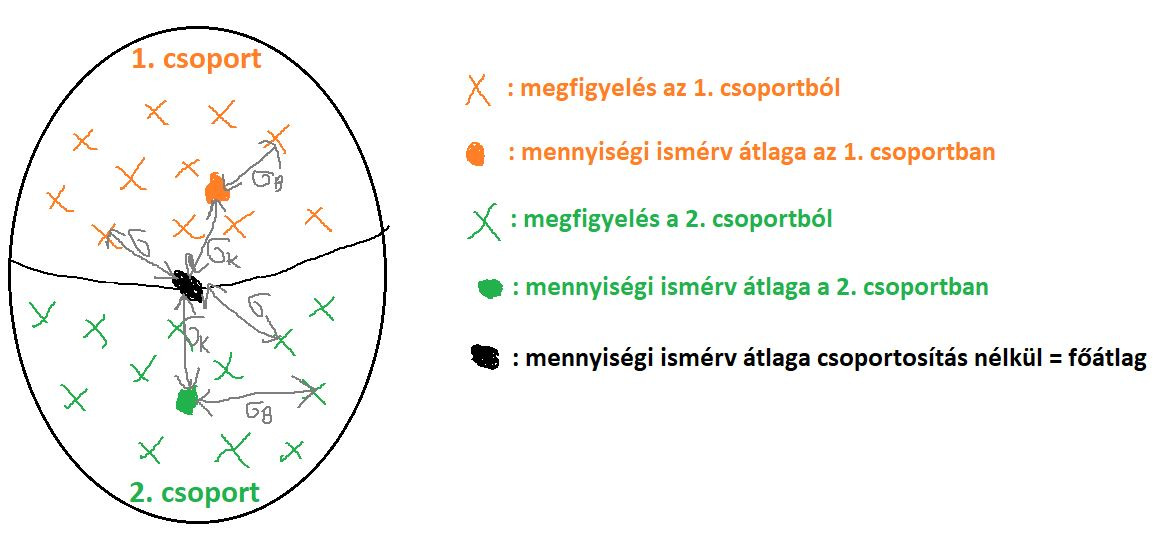
\includegraphics[width=0.8\textwidth,height=\textheight]{varhanyad1.jpg}

Tehát vizuálisan a következőképp érdemes gondolni a különböző \(\sigma\)-kra:

\begin{itemize}
\tightlist
\item
  \(\sigma_B\): Megfigyelések távolsága saját csoportjuk átlagától
\item
  \(\sigma_K\): Csoportátlag távolsága a főátlagtól
\item
  \(\sigma\): Megfigyelések távolsága a főátlagától
\end{itemize}

Ezek alapján nekünk az a jó a csoportosítás, azaz a minőségi ismérv magyarázóereje szempontjából, ha \textbf{fix} \(\sigma\) mellett \(\sigma_K\) \textbf{nagy} és \(\sigma_B\) \textbf{kicsi}. Mert ekkor a \textbf{csoportátlagok messze vannak} a főátlagtól és így implicite \textbf{egymástól} is, míg a csoportátlagtól az egyes \textbf{megfigyelések nagyon kis mértékben térnek csak el saját csoportátlaguktól}:

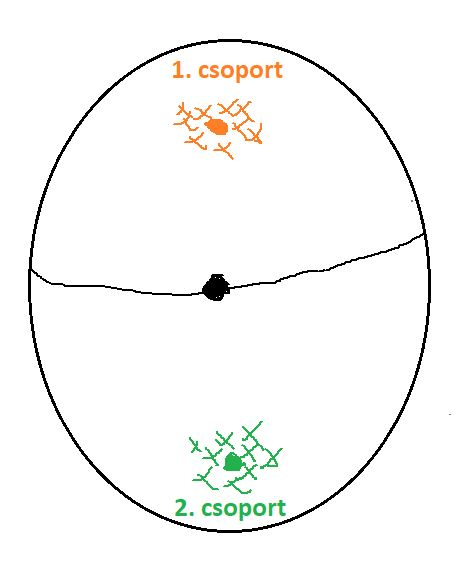
\includegraphics[width=0.3\textwidth,height=\textheight]{varhanyad2.jpg}

Ebben az esetben, ahogy az ábráról is látszik a csoportosításunk, azaz a minőségi ismérvünk magyarázóereje nagy! Tehát az kell nekünk, hogy az \(\sigma\) minél nagyobb részét tegye ki \(\sigma_K\). Viszont, mivel csak a teljes \textbf{varianciára} igaz az, hogy \textbf{egyenlő a külső és belső VARIANCIA összegével}, így azt mondjuk, hogy \textbf{azt szeretnénk látni}, hogy \textbf{a \(\frac{\sigma_K^2}{\sigma^2}\) hányados nagy legyen}! Ez a mutató lesz tehát a \textbf{varianciahányados}, és a most elvégzett módszer neve a \textbf{variancia-analízis, azaz ANOVA = ANalysis Of VAriances}.

\textbf{Azért a varianciákra néztük végül a dolgokat}, mert \(\sigma^2=\sigma_B^2+\sigma_K^2\), így a \(\frac{\sigma_K^2}{\sigma^2}\) variancia-hányados biztos, hogy \(0-1\) közötti, és \textbf{százalékosan} is értelmezhető, hiszen \(\sigma_K^2\) része \(\sigma^2\)-nek. Ez alapján nekünk most:

\(\frac{\sigma_K^2}{\sigma^2} = \frac{933.98387}{3996.64097}=0.23369=23.369\%\) --\textgreater{} \textbf{A hónap (tehát a Sound jelenléte) a Balatonban mért kokainmennyiség alakulásának (varianciájának) kb. 23\%-át magyarázza a megfigyelt adatok körében!} Ez egy \textbf{közepes magyarázóerő}nek tekinthető, mivel a variancia-hányadost a következőképpen ``\emph{korszakoljuk}'':

\begin{itemize}
\tightlist
\item
  \textbf{variancia-hányados \textless{} 10\% --\textgreater{} gyenge kapcsolat}
\item
  \textbf{10\% \textless= variancia-hányados \textless= 50\% --\textgreater{} közepes kapcsolat}
\item
  \textbf{variancia-hányados \textgreater{} 50\% --\textgreater{} erős/szoros kapcsolat}
\end{itemize}

\subsection{További minőségi ismérvek és a kokainmennyiség}\label{tovuxe1bbi-minux151suxe9gi-ismuxe9rvek-uxe9s-a-kokainmennyisuxe9g}

Az eredmény tehát azt mondja, hogy a kokainmennyiség alakulásának csak kb. \(23\%\)-át tudjuk csak lefedni azzal, hogy a mérés melyik hónapban készült. Tehát hónapkon \emph{belül} is jelentős mértékű szódósás maradt a mennyiségi ismérvünkben, jelesül a kokainmennyiségben.
Mi okozhatja még a kokainmennyiség szóródását? Hát, az elérhető adatok tekintetében két dolgot tudunk még megvizsgálni: azt, hogy \textbf{melyik mérőállomáson történt a mérés}, illetve azt, hogy \textbf{melyik évben}. Reméljük, hogy \emph{inkább az év magyarázza még relatíve nagyobb mértékben a kokainmennyiség alakulását} (pl. emelkedő trend tapasztalható a Sound népszerűségének növekedésével), mert \emph{ha a kokainmennyiség szóródása inkább a mérőállomástól függ}, az \emph{aggasztó lenne a mérés megbízhatóságára nézve}.

Mivel mind a mérőállomás azonosítója, mind az évszám jelen szituációban minőségi ismérvként kezelhető, így e két ismérvnek a kokainmennyiséggel, mint mennyiségi ismérvvel vett varianciahányadosát kell megvizsgálnunk.

Először nézzük a \textbf{mérőállomások esetét}.

Itt is kell ugyebár egy kiinduló segédtáblázat.

\begin{Shaded}
\begin{Highlighting}[]
\NormalTok{AllomasTabla }\OperatorTok{=}\NormalTok{ Balcsi.groupby(}\StringTok{\textquotesingle{}Allomas\textquotesingle{}}\NormalTok{).agg(}
\NormalTok{  Elemszam }\OperatorTok{=}\NormalTok{ (}\StringTok{\textquotesingle{}Kokain\textquotesingle{}}\NormalTok{, }\StringTok{\textquotesingle{}count\textquotesingle{}}\NormalTok{),}
\NormalTok{  Reszatlagok }\OperatorTok{=}\NormalTok{ (}\StringTok{\textquotesingle{}Kokain\textquotesingle{}}\NormalTok{, np.mean),}
\NormalTok{  Szorasok }\OperatorTok{=}\NormalTok{ (}\StringTok{\textquotesingle{}Kokain\textquotesingle{}}\NormalTok{, np.std)}
\NormalTok{).reset\_index()}
\end{Highlighting}
\end{Shaded}

\begin{verbatim}
## <string>:1: FutureWarning: The provided callable <function mean at 0x000001CA046C13A0> is currently using SeriesGroupBy.mean. In a future version of pandas, the provided callable will be used directly. To keep current behavior pass the string "mean" instead.
## <string>:1: FutureWarning: The provided callable <function std at 0x000001CA046C14E0> is currently using SeriesGroupBy.std. In a future version of pandas, the provided callable will be used directly. To keep current behavior pass the string "std" instead.
\end{verbatim}

\begin{Shaded}
\begin{Highlighting}[]
\NormalTok{AllomasTabla}
\end{Highlighting}
\end{Shaded}

\begin{verbatim}
##       Allomas  Elemszam  Reszatlagok   Szorasok
## 0  1. állomás       180    30.101843  84.544224
## 1  2. állomás       180    22.314141  61.220808
## 2  3. állomás       180    12.502428  30.877849
\end{verbatim}

Olybá tűnik, hogy az 1. állomás átlagban némileg kicsit magasabb kokainmenyniséget mér, mint a többi, de az állomás méréseinek szórása is magas, az átlagos kokainmennyiség kb. \(\frac{84.5}{30.1}=2.8\)-szorosa.
Szóval, vágjunk rendet a variancia-hányados segítségével, és lássuk mekkora hatást gyakorol a mérőállomás a kokainmennyiségre!

A számításokban annyi \textbf{egyszerűsítés}t teszek, hogy

\begin{itemize}
\tightlist
\item
  A \textbf{teljes varianciát örökítem} az előző számolásokból, hiszen az a csoportosítás alapját képzőú minőpségi ismérv megváltozásával \textbf{nem változik}.
\item
  Az előző pont és a belső variancia kiszámolása után pedig a varianciahányadost a \(\sigma^2=\sigma_B^2+\sigma_K^2\) összefüggás átrendezésével \(H^2=\frac{\sigma^2-\sigma_B^2}{\sigma^2}=1-\frac{\sigma_B^2}{\sigma^2}\) módon számolom ki
\end{itemize}

Ezzel a két módosítással \textbf{megúszom a külső szórásnégyzet} kissé macerás \textbf{kiszámítását}.

\begin{Shaded}
\begin{Highlighting}[]
\NormalTok{belső\_var\_Állomás }\OperatorTok{=}\NormalTok{ np.}\BuiltInTok{sum}\NormalTok{(AllomasTabla.Elemszam }\OperatorTok{*}\NormalTok{ AllomasTabla.Szorasok}\OperatorTok{**}\DecValTok{2}\NormalTok{)}\OperatorTok{/}\NormalTok{np.}\BuiltInTok{sum}\NormalTok{(AllomasTabla.Elemszam)}

\NormalTok{VarHányadÁllomás }\OperatorTok{=} \DecValTok{1} \OperatorTok{{-}}\NormalTok{ belső\_var\_Állomás }\OperatorTok{/}\NormalTok{ teljes\_var}
\NormalTok{VarHányadÁllomás}
\end{Highlighting}
\end{Shaded}

\begin{verbatim}
## 0.01174053573946432
\end{verbatim}

Az eredmény mindössze \(1.17\%\). Tehát megnyugodhatunk, az \textbf{állomás a mért kokainmennyiség alakulását csak alig több, mint 1\%-ban határozza meg}! A \textbf{mérés nem függ lényegében az állomástól}, így ilyen szempointból megbízhatónak tekintehtők!

Lássuk az \textbf{évszámok}at! Most is kezdjük a segédtáblával.

\begin{Shaded}
\begin{Highlighting}[]
\NormalTok{EvTabla }\OperatorTok{=}\NormalTok{ Balcsi.groupby(}\StringTok{\textquotesingle{}Ev\textquotesingle{}}\NormalTok{).agg(}
\NormalTok{  Elemszam }\OperatorTok{=}\NormalTok{ (}\StringTok{\textquotesingle{}Kokain\textquotesingle{}}\NormalTok{, }\StringTok{\textquotesingle{}count\textquotesingle{}}\NormalTok{),}
\NormalTok{  Reszatlagok }\OperatorTok{=}\NormalTok{ (}\StringTok{\textquotesingle{}Kokain\textquotesingle{}}\NormalTok{, np.mean),}
\NormalTok{  Szorasok }\OperatorTok{=}\NormalTok{ (}\StringTok{\textquotesingle{}Kokain\textquotesingle{}}\NormalTok{, np.std)}
\NormalTok{).reset\_index()}
\end{Highlighting}
\end{Shaded}

\begin{verbatim}
## <string>:1: FutureWarning: The provided callable <function mean at 0x000001CA046C13A0> is currently using SeriesGroupBy.mean. In a future version of pandas, the provided callable will be used directly. To keep current behavior pass the string "mean" instead.
## <string>:1: FutureWarning: The provided callable <function std at 0x000001CA046C14E0> is currently using SeriesGroupBy.std. In a future version of pandas, the provided callable will be used directly. To keep current behavior pass the string "std" instead.
\end{verbatim}

\begin{Shaded}
\begin{Highlighting}[]
\NormalTok{EvTabla}
\end{Highlighting}
\end{Shaded}

\begin{verbatim}
##      Ev  Elemszam  Reszatlagok   Szorasok
## 0  2017       180     0.536273   0.734331
## 1  2018       180     1.964270   3.933046
## 2  2019       180    62.417870  97.366788
\end{verbatim}

Itt azért elég látványos eltéréseket találunk! A 2019-es évben hatalmasat ugrott a Balatonban mérhető kokainmennyiség. A szórása is magas, de pl. relatíve nézve 2018-ban magasabb volt: 2018-ban a szórás durván kétszerese volt az átlagnak \(\frac{3.93}{1.96}\), míg 2019-ben csak durván másfélszerese \(\frac{97.37}{62.42}=1.56\). Szóval itt lehet még komolyabb magyarázóerő!
De ne találgassunk, hanem lássuk a varianciahányadost! A számolásnál megint alkalmazzuk az állomásoknál bevezetett két \textbf{egyszerűsítés}t!

\begin{Shaded}
\begin{Highlighting}[]
\NormalTok{belső\_var\_Év }\OperatorTok{=}\NormalTok{ np.}\BuiltInTok{sum}\NormalTok{(EvTabla.Elemszam }\OperatorTok{*}\NormalTok{ EvTabla.Szorasok}\OperatorTok{**}\DecValTok{2}\NormalTok{)}\OperatorTok{/}\NormalTok{np.}\BuiltInTok{sum}\NormalTok{(EvTabla.Elemszam)}

\NormalTok{VarHányadÉv }\OperatorTok{=} \DecValTok{1} \OperatorTok{{-}}\NormalTok{ belső\_var\_Év }\OperatorTok{/}\NormalTok{ teljes\_var}
\NormalTok{VarHányadÉv}
\end{Highlighting}
\end{Shaded}

\begin{verbatim}
## 0.20797660221119585
\end{verbatim}

Na, itt is egy közepes magyarázóerőnk van, kb. \(21\%\).

Tehát alapvetően a Balatonban mérhető kokainmennyiséget két \emph{közepes magyarázóerejű} dolog mozgatja nyáron:

\begin{itemize}
\tightlist
\item
  \textbf{Hónap}: A Balaton Sound hónapjában (július) átlagban valamivel több a kokain
\item
  \textbf{Év}: 2019-ben sokkal több az átlagos kokainmennyiség, feltehetően a Sound megnövekedett haza és külföldi népszerűsége miatt
\end{itemize}

Szerencsére a mérőállomás maga nem befolyásolja érdemben a mért kokain szóródását, így a mérések ilyen szempontból megbízhatóank tekinthetők!

\chapter{Eloszlások és Mintavételezés}\label{eloszluxe1sok-uxe9s-mintavuxe9telezuxe9s}

\section{Véletlenszám generálás és Mintavételezés}\label{vuxe9letlenszuxe1m-generuxe1luxe1s-uxe9s-mintavuxe9telezuxe9s}

Minden programnyelv alapelemének számít egy olyan függvény, ami \(0-1\) értékek közötti véletlen számokat generál. Egész pontosan ezek a függvények \textbf{úgy generálnak számokat, hogy azok \(0-1\) között minden értéket azonos valószínűséggel}, tehát \textbf{egyenletes eloszlással} vehetnek fel.
Az ilyen \(0-1\) között egyenletes eloszlású véletlenszám generátorok minden programnyelv alapvető eszközei, és a Számítástudományból tanult lineáris kongruenciarendszereken alapulnak.

A \(0-1\) közötti teljesen véletlen számok generálásához Pythonban egy \texttt{random} c.~csomagot kell importálni, és ennek a (nem meglepő módon) \texttt{random} névre keresztelt függvényével tudunk véletlen számokat dobálgatni.

\begin{Shaded}
\begin{Highlighting}[]
\ImportTok{import}\NormalTok{ random}

\NormalTok{GondoltamEgySzámra }\OperatorTok{=}\NormalTok{ random.random()}
\NormalTok{GondoltamEgySzámra}
\end{Highlighting}
\end{Shaded}

\begin{verbatim}
## 0.4739292112581075
\end{verbatim}

Fenti kódsort futtatva nyilván mindenkinek más eredménye lesz, hiszen \emph{random} számot generálunk. :) A lényeg, hogy a számunk \(0-1\) közötti!

Node, \textbf{mit csinál ez a véletlenszám generátor statisztikus szemmel tekintve}? Nos, ilyenkor ők \textbf{egy olyan \(Y_i\) adatsorból húznak véletlenszerűen egy \(x\) számértéket, aminek az eloszlása \(0-1\) közötti egyenletes eloszlás}. Ennek a matematikai jelölésrendszere: \(Y_i \sim U(0,1)\). Az \(U\) onnan jön, hogy az egyenletes eloszlás in English \emph{uniform distribution}.

Húzzunk akkor most ebből a \(Y_i \sim U(0,1)\) adatsorból \(50\) db véletlen értéket, és tároljuk el az eredményeket egy Python \texttt{list} objektumban! Azaz, \textbf{vegyünk a \(U(0,1)\) eloszlásból egy \(n=50\) elemű mintát!}

Technikailag úgy kell eljárnunk, hogy létrhozunk egy üres listát Pythonban, és az \texttt{append} metódusa segítségével föltöltjük \(50\) db random \(0-1\) közötti számmal.

\begin{Shaded}
\begin{Highlighting}[]
\NormalTok{SzerencsétlenVéletlenek }\OperatorTok{=}\NormalTok{ [] }\CommentTok{\# üres lista létrehozása}

\ControlFlowTok{for}\NormalTok{ index }\KeywordTok{in} \BuiltInTok{range}\NormalTok{(}\DecValTok{50}\NormalTok{):}
\NormalTok{  SzerencsétlenVéletlenek.append(random.random()) }\CommentTok{\# véletlen szám hozzáadása a listához}

\NormalTok{SzerencsétlenVéletlenek}
\end{Highlighting}
\end{Shaded}

\begin{verbatim}
## [0.3036673091206754, 0.9554664893312815, 0.8901607222030957, 0.039783618666481724, 0.14790059603681915, 0.5212547134803249, 0.01789182344330198, 0.6799397634010272, 0.060987056344302126, 0.4772318958384323, 0.5713941464643092, 0.8227869855479997, 0.35852836313231573, 0.18903819986727088, 0.24586349635315952, 0.9947267327809628, 0.3386296706790499, 0.5036097799360871, 0.5075973687496721, 0.4907738205523604, 0.8528605144213413, 0.4939481604847631, 0.15960532446211584, 0.5862917657279939, 0.8970708832621047, 0.9927230298987798, 0.8049266814161122, 0.44131912586249367, 0.2638227949396871, 0.39435118739569064, 0.24022474663566984, 0.3126231584544116, 0.28333081964872964, 0.8806355988250284, 0.04407488259122494, 0.9299877357341024, 0.42591010091724013, 0.07093876751841077, 0.33482854246925353, 0.22585846900071882, 0.7752913830438778, 0.7802885846414015, 0.19054596129145118, 0.6000783161662636, 0.7050559608150839, 0.4807127993687077, 0.25866536928497985, 0.4554557295970433, 0.8311132401483492, 0.48823119861236874]
\end{verbatim}

Itt is van az \(50\) szép kicsi véletlen számom. Nyilván ezek megint mindenkinek más értékek. :)

Következő lépésben \textbf{ezt az \(50\) elemű mintát transzformáljuk át olyanná, hogy ne egy \(U(0,1)\) eloszlásból, hanem mondjuk egy \(U(40,160)\) eloszlásból származó minta}! Magyarul, az kéne, hogy ez az \(50\) véletlen szám, ne \(50\) db \(0-1\) közötti véletlen szám, hanem \(50\) db \(40-160\) közötti véletlen szám legyen!

Ezt a következőképpen tudjuk elérni:

\begin{itemize}
\tightlist
\item
  Ha a \(0-1\) közti véletlenszámokat megszorozzuk \(160-40=120\)-szal, akkor \(0-120\) közti véletlen számok lesznek.
\item
  Ha a \(0-120\) közti véletlen számokhoz hozzáadunk \(40\)-et, akkor \((0+40)\) és \((120+40)\) közti, azaz \(40-160\) közti véletlen számok leszenek.
\end{itemize}

Ahhoz, hogy ezt technikailag kivitelezni tudjuk a \texttt{s} listánkat először \texttt{numpy} tömbbé kell konvertálni. De utána elég egyszerűen menni fog a dolog.

\begin{Shaded}
\begin{Highlighting}[]
\ImportTok{import}\NormalTok{ numpy }\ImportTok{as}\NormalTok{ np}

\NormalTok{SzerencsétlenVéletlenek }\OperatorTok{=}\NormalTok{ np.array(SzerencsétlenVéletlenek)}
\NormalTok{SzerencsétlenVéletlenek }\OperatorTok{=}\NormalTok{ (SzerencsétlenVéletlenek }\OperatorTok{*}\NormalTok{ (}\DecValTok{160}\OperatorTok{{-}}\DecValTok{40}\NormalTok{)) }\OperatorTok{+} \DecValTok{40}
\NormalTok{SzerencsétlenVéletlenek}
\end{Highlighting}
\end{Shaded}

\begin{verbatim}
## array([ 76.44007709, 154.65597872, 146.81928666,  44.77403424,
##         57.74807152, 102.55056562,  42.14701881, 121.59277161,
##         47.31844676,  97.2678275 , 108.56729758, 138.73443827,
##         83.02340358,  62.68458398,  69.50361956, 159.36720793,
##         80.63556048, 100.43317359, 100.91168425,  98.89285847,
##        142.34326173,  99.27377926,  59.15263894, 110.35501189,
##        147.64850599, 159.12676359, 136.59120177,  92.9582951 ,
##         71.65873539,  87.32214249,  68.8269696 ,  77.51477901,
##         73.99969836, 145.67627186,  45.28898591, 151.59852829,
##         91.10921211,  48.5126521 ,  80.1794251 ,  67.10301628,
##        133.03496597, 133.63463016,  62.86551535, 112.00939794,
##        124.6067153 ,  97.68553592,  71.03984431,  94.65468755,
##        139.73358882,  98.58774383])
\end{verbatim}

Olybá tűnik a foglalkozásunk elérte célját: tényleg nincs itt \(40\)-nél kisebb és \(160\)-nál nagyobb szám! :)

Nézzük meg, hogy mennyire egyenletes eloszlásúak a generált \(U(40,160)\) eloszlású számaink! Rajzoljuk ki a hisztogramot!
Ehhez kelleni fog a \texttt{matplotlib} csomag \texttt{hist} függvénye is. Eza függvény lényegében a \texttt{numpy} csomag \texttt{histogram} függvénye, de listákra csak ezt lehet alkalmazni. Ugyebár még nem mentettük a dolgokat \texttt{pandas} data frame-be, ezért ilyen körülményes kicsit a hisztogram rajzolás.
Mivel \(50\) adatot generáltunk, így a hisztogramhoz \(k=6\) osztályköz kell a \(2^k \geq N\) szabály alapján (\(2^6=64\))

\begin{Shaded}
\begin{Highlighting}[]
\ImportTok{import}\NormalTok{ matplotlib.pyplot }\ImportTok{as}\NormalTok{ plt}

\NormalTok{Hisztogram }\OperatorTok{=}\NormalTok{ plt.hist(SzerencsétlenVéletlenek, bins }\OperatorTok{=} \DecValTok{6}\NormalTok{)}
\NormalTok{plt.show()}
\end{Highlighting}
\end{Shaded}

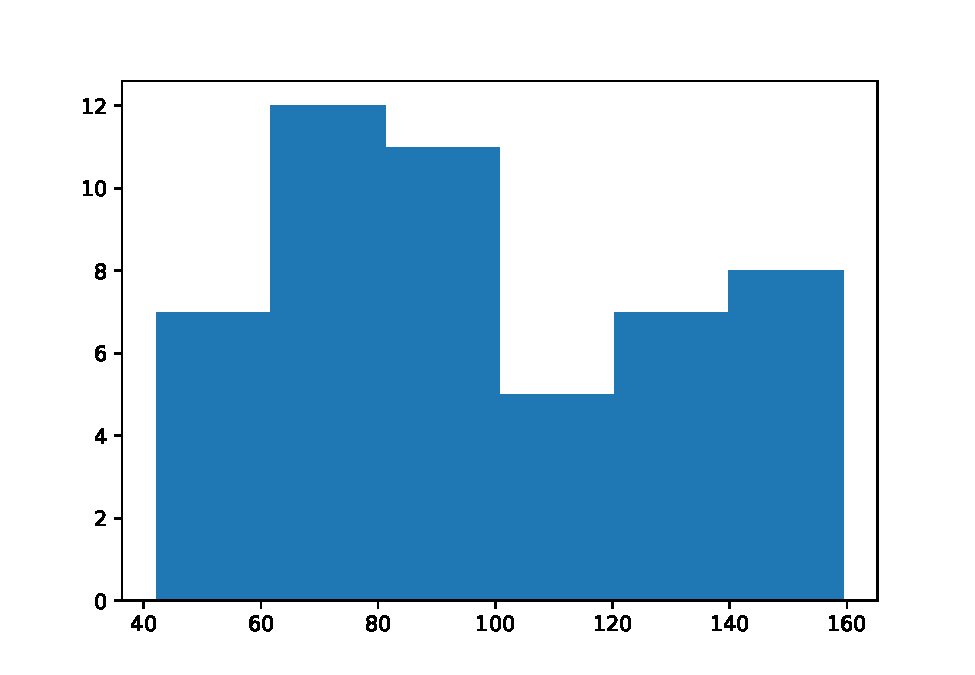
\includegraphics{_main_files/figure-latex/unnamed-chunk-205-3.pdf}

Mit is kéne látni ezen a hisztogramon? Hát általánossában az \(U(a,b)\) eloszlás, azaz az \((a,b)\) intervallumon egyenletes eloszlás sűrűségfüggvénye \(f(x) = \frac{1}{b-a}\), hiszen a sűrűségfüggvény helyettesítési értéke az egy konkrét \(x\) érték bekövetkezési valószínűsége az \(U(a,b)\) eloszlásban, \(P(Y_i=x)\). Ami az egyenletes eloszlás esetén minden \(x\)-re \(a-b\) között ugyan annyi, nevezetesen ``\emph{1 per az \((a,b)\) intervallum hossza}!

Esetünkben tehát \textbf{az \(U(40,160)\) eloszlás sűrűségfüggvénye} az \(f(x)=\frac{1}{160-40}=\frac{1}{120}=0.0083\) magasságban futó \textbf{vízszintes egyenes}. Vagyis \textbf{a hisztogramnak minden \(x\) értékre kb. ugyan akkora gyakoriságot kell mutatnia, ami azért szemmel láthatóan nem így van!}

\textbf{Rajzoljuk csak ki a hisztogramot \texttt{density\ =\ True} beállítással és véssük fel rá az \(U(40,160)\) eloszlás sűrűségfüggvényét!} Ezt az ábrát hasonlóan lehet elkészíteni, mint ahogy a normális eloszlás sűrűségfüggvény illeszkedését vizsgáltuk garfikusan a Tesla árváltozások hisztogramjára az 1. heti tananyag 2.3. fejezet végén.
Sőt, természetesen a \texttt{scipy} csomag \texttt{stats} névterének \texttt{uniform.pdf} függvényével is ki tudjuk számolni az \(U(40,160)\) eloszlás konstans \(f(x)=0.0083\)-as sűrűségfüggvényét, ahogy az 1. heti anyagban kiszámoltuk a normális eloszlás sűrűségfüggvény \(f(x)\) értékeit a \texttt{norm.pdf} függvénnyel. Arra kell figyelni az \texttt{uniform.pdf} függvénynél, hogy a \texttt{loc} nevű paraméterben kell megadni az \(U(a,b)\) eloszlás alsó határát, azaz \(a\)-t, míg a \texttt{scale} paraméterben a \textbf{terjedelemét}, azaz az \(a-b=160-40=120\)-at!

\begin{Shaded}
\begin{Highlighting}[]
\ImportTok{import}\NormalTok{ scipy.stats }\ImportTok{as}\NormalTok{ stats}

\NormalTok{eloszlás\_alsó\_határ }\OperatorTok{=} \DecValTok{40}
\NormalTok{eloszlás\_felső\_határ }\OperatorTok{=} \DecValTok{160}
\NormalTok{eloszlás\_terjedelem }\OperatorTok{=}\NormalTok{ eloszlás\_felső\_határ }\OperatorTok{{-}}\NormalTok{ eloszlás\_alsó\_határ}

\NormalTok{Hisztogram }\OperatorTok{=}\NormalTok{ plt.hist(SzerencsétlenVéletlenek, bins }\OperatorTok{=} \DecValTok{6}\NormalTok{, density }\OperatorTok{=} \VariableTok{True}\NormalTok{)}
\NormalTok{x\_tengely }\OperatorTok{=}\NormalTok{ np.arange(eloszlás\_alsó\_határ, eloszlás\_felső\_határ, }\FloatTok{0.01}\NormalTok{)}
\NormalTok{y\_tengely }\OperatorTok{=}\NormalTok{ stats.uniform.pdf(x }\OperatorTok{=}\NormalTok{ x\_tengely, loc }\OperatorTok{=}\NormalTok{ eloszlás\_alsó\_határ,scale }\OperatorTok{=}\NormalTok{ eloszlás\_terjedelem)}
\NormalTok{plt.plot(x\_tengely, y\_tengely)}
\NormalTok{plt.show()}
\end{Highlighting}
\end{Shaded}

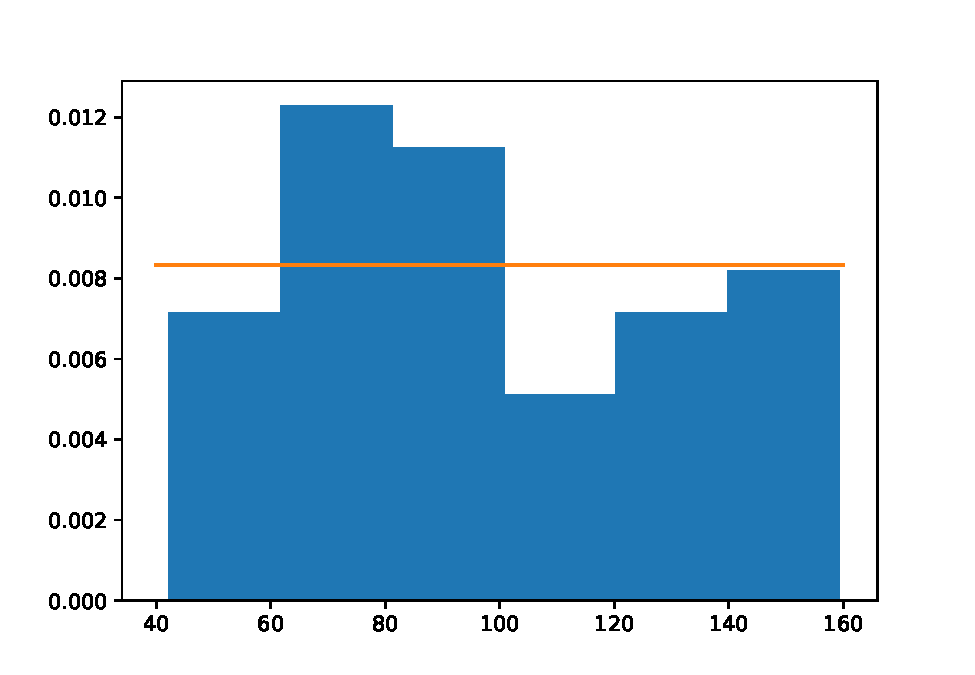
\includegraphics{_main_files/figure-latex/unnamed-chunk-206-5.pdf}

Láthatjuk azért, hogy az \(50\) elemű \textbf{minta tapasztalt gyakoriságai nem annyira tükrözik az egyenletes eloszlás} vízszintes \(f(x) = 0.0083\) magas \textbf{sűrűségfüggvényét, de azért többnyire a függvény vonala körül mozognak}. Azt pedig már lecsekkoltuk, hogy a vgenerált minta minden értéke tényleg a \((40,160)\) intervallumban található, de ez most szépen látszik a hisztogram \(x\) tengelyén is.

Tehát, sikeresen \textbf{eltranszformáltuk az \(U(0,1)\) eloszlású \(50\) elemű mintánkat \(U(40,160)\) eloszlásúvá}. Mindjárt látjuk, hogy \textbf{az \(U(0,1)\) eloszlású véletlen számokat nem csak egy másik egyenletes \(U(a,b)\) eloszlásúvá, hanem tetszőleges eloszlásúvá is tudjuk tarnszformálni!!}

\subsection{A mintagenerálás általános elve}\label{a-mintageneruxe1luxe1s-uxe1ltaluxe1nos-elve}

Gondolkozzunk el azon, hogyan is lehet \textbf{formalizálni azt a képletet, amivel az \(U(0,1)\) eloszlású véletlen számokból U(a,b) eloszlású véletlen számokat csináltunk!}
Ugyebár a generált számot megszoroztuk az \((a,b)\) intervallum hosszával, és hozzáadtuk az alsó határt, \(a\)-t. Azaz formálisan azt mondhatjuk, hogy ha \(y \sim U(0,1)\), akkor \(z = y \times (b-a) + a \sim U(a,b)\).

De honnan is jön ez a képlet? \textbf{Gondoljunk bele, hogy \(U(a,b)\) eloszlás esetén hogyan is számolunk ki egy \(P(Y_i < x)\) ``alá esési'' valószínűséget?} Azaz, mi a \(\int_{-\infty}^x{\frac{1}{b-a}}dx\) improprius integrál eredménye?

Ez azért nem olyan bonyi vállalkozás, mint mondjuk egy normális eloszlás esetén kiszámolni a cuccot, hiszen mivel \(a\) alatt az \(a-b\) közötti egyenletes eloszlásban \(0\) valószínűséggel lehetnek értékek, így az improprius integrálunk rögtön határozott integrállá válik:\(\int_a^x{\frac{1}{b-a}}dx\). Ezzel pedig már könnyen elbánunk, hiszen az integrálandó függvényben nincs is benne a függvény változója, az \(x\), tehát konstans függvényről van szó: \[\int_a^x{\frac{1}{b-a}}dx=\left[\frac{x}{b-a}\right]_a^x=\frac{x}{b-a}-\frac{a}{b-a}=\frac{x-a}{b-a}\]

Az eredmény szemléletesen persze az alábbi téglalap területe, hiszen a két oldal hossza \(oldal_1=x-a\), illetve a sűrűségfüggvény maga \(oldal_2=f(x)=\frac{1}{b-a}\) és a téglalap területe \(T=oldal_1 \times oldal_2 = (x-a) \times\frac{1}{b-a} = \frac{x-a}{b-a}\)

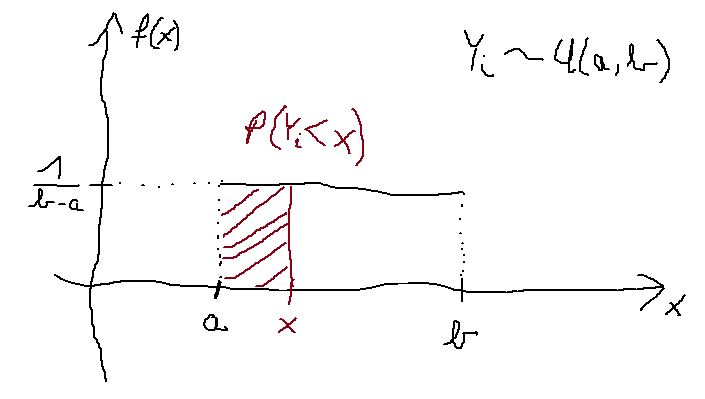
\includegraphics[width=0.6\textwidth,height=\textheight]{unifelo.jpg}

Szóval, ha \textbf{véletlenszerűen húzok egy \(Y_i\) számot az \(U(a,b)\) eloszlásból, akkor annak a valószínűsége, hogy \(x\)-nél kisebb értéket kapok nem más, mint \(P(Y_i < x) = \frac{x-a}{b-a}\).}

Nagyon jó. Akkor, \textbf{nézzük meg mi most az inverz függvény az egyenletes eloszlásban!} Azaz hogyan válaszolom meg azt a kérdést mi szerint: \textbf{Mi az az érték, aminél csak \(5\%\) valószínűséggel kapok kisebb értéket egy \(U(a,b)\) eloszlásban?}

Ugye ekkor az \(P(Y_i < x) = \frac{x-a}{b-a}\) összefüggésből kéne kifejeznem \(x\)-et, ami aránylag könnyű művelet: \[x=P(Y_i < x) \times (b-a) + a\]

\textbf{Hoppácska!} Amit kaptunk az gyakorlatilag \textbf{ugyan az a formula, amivel a \(y \sim U(0,1)\) eloszlásból \(z \sim U(a,b)\) eloszlást csináltunk}: \(z = y \times (b-a) + a\)

Tehát, \textbf{általánosságban azt az eredményt kapjuk, hogy ha egy \(U(0,1)\) eloszlású véletlen számra \(P(Y_i < x)\) valószínűségként tekintek, és berakom azt egy tetszőleges eloszlás inverz függvényébe, és megkeresem a hozzá tartozó \(x\) értéket, akkor amit kapok eredményül az olyan eloszlású véletlen szám lesz, mint amilyen eloszlás inverz függvényébe beírtam az \(U(0,1)\) eloszlású véletlen számot!!}
Ugyebár simán tekinthetek egy \(0-1\) közötti véletlenszámra \(P(Y_i < x)\) valószínűségként, hiszen minden valószínűség egy \(0-1\) közötti szám. :)

\textbf{Nézzük is meg az elvet a gyakorlatban!} Ugye a \texttt{scipy} csomagban minden eloszlás inverz függvényét a \texttt{ppf} rövidítésű függvénnyel számoltuk ki (lásd 1. heti tananyag 2.5. fejezetben).

\begin{Shaded}
\begin{Highlighting}[]
\NormalTok{eloszlás\_alsó\_határ }\OperatorTok{=} \DecValTok{40}
\NormalTok{eloszlás\_felső\_határ }\OperatorTok{=} \DecValTok{160}
\NormalTok{eloszlás\_terjedelem }\OperatorTok{=}\NormalTok{ eloszlás\_felső\_határ }\OperatorTok{{-}}\NormalTok{ eloszlás\_alsó\_határ}

\CommentTok{\# Leürítjük a korábbi véletlenszámaink listáját és új üres listát hozunk létre}
\NormalTok{SzerencsétlenVéletlenek }\OperatorTok{=}\NormalTok{ []}

\CommentTok{\# 50 db U(0,1) eloszlású szám generálása}
\ControlFlowTok{for}\NormalTok{ index }\KeywordTok{in} \BuiltInTok{range}\NormalTok{(}\DecValTok{50}\NormalTok{):}
\NormalTok{  SzerencsétlenVéletlenek.append(random.random()) }\CommentTok{\# véletlen szám hozzáadása a listához}

\CommentTok{\# U(40,160){-}á transzformálás inverz függvénnyel}
\NormalTok{SzerencsétlenVéletlenek }\OperatorTok{=}\NormalTok{ stats.uniform.ppf(}
\NormalTok{  SzerencsétlenVéletlenek,}
\NormalTok{  loc }\OperatorTok{=}\NormalTok{ eloszlás\_alsó\_határ,}
\NormalTok{  scale }\OperatorTok{=}\NormalTok{ eloszlás\_terjedelem)}

\CommentTok{\# Eredmény ellenőrzése hisztogramon}
\NormalTok{Hisztogram }\OperatorTok{=}\NormalTok{ plt.hist(SzerencsétlenVéletlenek, bins }\OperatorTok{=} \DecValTok{6}\NormalTok{, density }\OperatorTok{=} \VariableTok{True}\NormalTok{)}
\NormalTok{x\_tengely }\OperatorTok{=}\NormalTok{ np.arange(eloszlás\_alsó\_határ, eloszlás\_felső\_határ, }\FloatTok{0.01}\NormalTok{)}
\NormalTok{y\_tengely }\OperatorTok{=}\NormalTok{ stats.uniform.pdf(x }\OperatorTok{=}\NormalTok{ x\_tengely, loc }\OperatorTok{=}\NormalTok{ eloszlás\_alsó\_határ,scale }\OperatorTok{=}\NormalTok{ eloszlás\_terjedelem)}
\NormalTok{plt.plot(x\_tengely, y\_tengely)}
\NormalTok{plt.show()}
\end{Highlighting}
\end{Shaded}

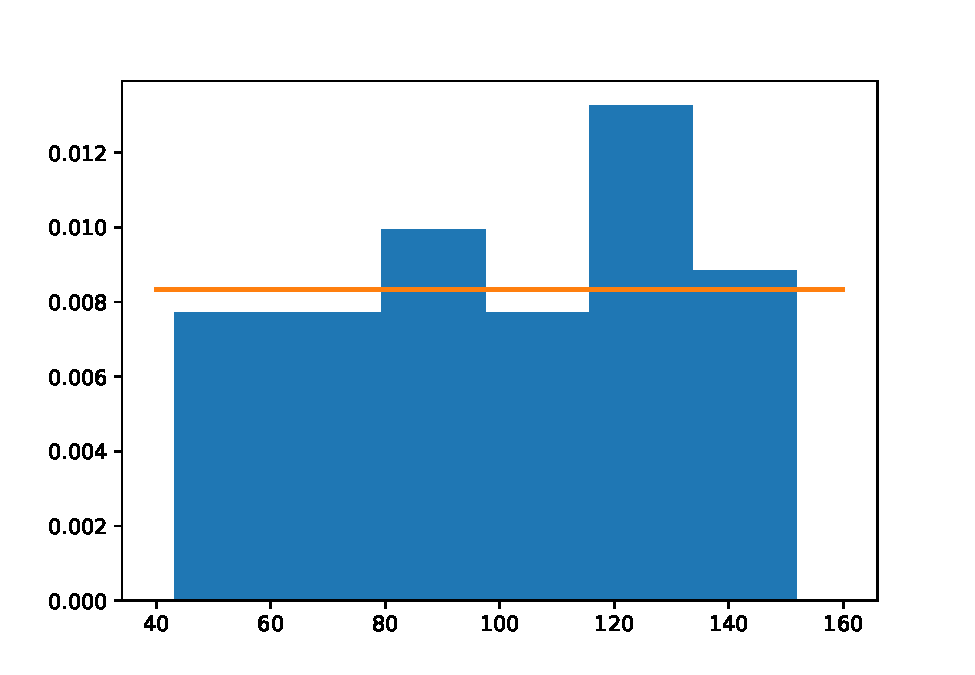
\includegraphics{_main_files/figure-latex/unnamed-chunk-207-7.pdf}

E voilá: siker! Az értékek \(40-160\) között mozognak, és a generált minta gyakoriságai kb. az \(U(40,160)\) eloszlás \(f(x)\) sűrűségfüggvénye körül ingadoznak!

\subsection{Nem egyenletes eloszlású minták generálása}\label{nem-egyenletes-eloszluxe1suxfa-mintuxe1k-generuxe1luxe1sa}

Na, akkor abban bízunk, hogy \textbf{az egyenletes eloszlás esetében megfigyelt trükk működni fog más eloszlásokra is}.

Tehát, \textbf{ha egy \(U(0,1)\) eloszlású véletlen számot berakom egy tetszőleges eloszlás inverz függvényébe, akkor amit eredményül kapok az olyan eloszlású véletlen szám, mint amilyen eloszlás inverz függvényébe beírtam az kezdeti \(U(0,1)\) eloszlású véletlen számot!!}

\textbf{Generáljunk akkor mondjuk először egy \(N(80,20)\) eloszlású \(50\) elemű mintát!} Tehát, a normális eloszlásunk átlaga \(\mu=80\) és szórása \(\sigma = 20\). A kezdeti \(U(0,1)\) számok transzformálására pedig használhatjuk akkor a \texttt{scipy} csomag \texttt{norm.ppf} függvényét.
Figyeljünk, hogy a sűrűségfüggvény rajzolásakor az \(x\) tengely alsó-felső határait már a generált adatokból szedjük, mert az elvi eloszlás alapján nem lehet itt megmondani! --\textgreater{} Nem \(U(a,b)\) egyenletes eloszlásunk van már \emph{úgymond}. :)

\begin{Shaded}
\begin{Highlighting}[]
\NormalTok{átlag }\OperatorTok{=} \DecValTok{80}
\NormalTok{szórás }\OperatorTok{=} \DecValTok{20}

\CommentTok{\# Leürítjük a korábbi véletlenszámaink listáját és új üres listát hozunk létre}
\NormalTok{SzerencsétlenVéletlenek }\OperatorTok{=}\NormalTok{ []}

\CommentTok{\# 50 db U(0,1) eloszlású szám generálása}
\ControlFlowTok{for}\NormalTok{ index }\KeywordTok{in} \BuiltInTok{range}\NormalTok{(}\DecValTok{50}\NormalTok{):}
\NormalTok{  SzerencsétlenVéletlenek.append(random.random()) }\CommentTok{\# véletlen szám hozzáadása a listához}

\CommentTok{\# N(80,20){-}á transzformálás inverz függvénnyel}
\NormalTok{Normika }\OperatorTok{=}\NormalTok{ stats.norm.ppf(}
\NormalTok{  SzerencsétlenVéletlenek,}
\NormalTok{  loc }\OperatorTok{=}\NormalTok{ átlag,}
\NormalTok{  scale }\OperatorTok{=}\NormalTok{ szórás)}

\CommentTok{\# Eredmény ellenőrzése hisztogramon}
\NormalTok{Hisztogram }\OperatorTok{=}\NormalTok{ plt.hist(Normika, bins }\OperatorTok{=} \DecValTok{6}\NormalTok{, density }\OperatorTok{=} \VariableTok{True}\NormalTok{)}
\NormalTok{x\_tengely }\OperatorTok{=}\NormalTok{ np.arange(np.}\BuiltInTok{min}\NormalTok{(Normika), np.}\BuiltInTok{max}\NormalTok{(Normika), }\FloatTok{0.01}\NormalTok{)}
\NormalTok{y\_tengely }\OperatorTok{=}\NormalTok{ stats.norm.pdf(x }\OperatorTok{=}\NormalTok{ x\_tengely, loc }\OperatorTok{=}\NormalTok{ átlag, scale }\OperatorTok{=}\NormalTok{ szórás)}
\NormalTok{plt.plot(x\_tengely, y\_tengely)}
\NormalTok{plt.show()}
\end{Highlighting}
\end{Shaded}

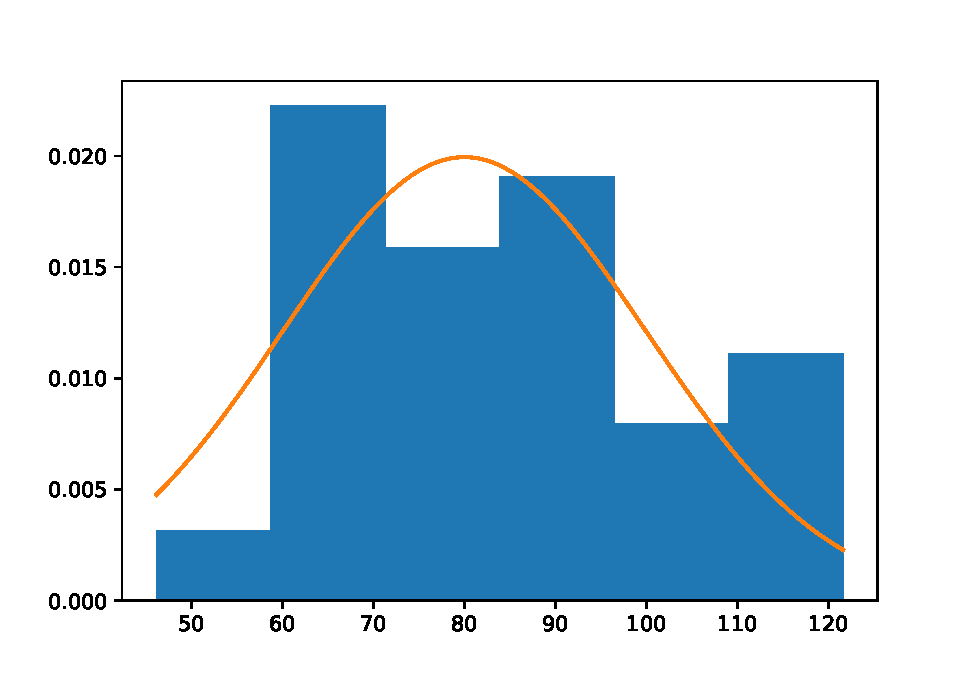
\includegraphics{_main_files/figure-latex/unnamed-chunk-208-9.pdf}

Na, egészen jól illeszkednek a generált adatok gyakoriságai a normális eloszlás sűrűségfüggvényéhez! :)

Természetesen, expoenciális eloszlásra is hasonlóan működik a trükk, de azt már nem nagy \emph{copy-paste mágia} lenne lekódolni. :)

A lényeg viszont, hogy ez a megoldás tényleg \textbf{minden létező eloszlásra működik!} Olyanokra is, amik \textbf{nincsenek benne} a \texttt{scipy}-ban!! Csak \textbf{tudni kell az eloszlás inverz függvényének képletét, és abba beírogatva \(U(0,1)\) eloszlású számokat, le is generáltunk egy mintát az eloszlásból!}

A jó hír viszont, hogy a \texttt{scipy}-ban szereplő eloszlásoknak van egy \texttt{rvs} álnevű függvénye, ami \textbf{automatikusan eljátsza a fenti trükköt, így nem kell} az eddig használt hosszabb kódrészletet \textbf{mindig copy-pastelni}. A függvényben az aktuális eloszlásnak (egyenletes, normális, exponenciális vagy más) megfelelő módon kell megadni a \texttt{loc} és \texttt{scale} paramétereket, míg a generálandó számok mennyiségét (a minta elemszámát) a \texttt{size} paraméterben lehet beállítani.

Tehát, egyszerűsítve az alábbi módon is lehet pl. \(U(40,160)\) eloszlűsú adatokat (mintát) generálni.

\begin{Shaded}
\begin{Highlighting}[]
\NormalTok{eloszlás\_alsó\_határ }\OperatorTok{=} \DecValTok{40}
\NormalTok{eloszlás\_felső\_határ }\OperatorTok{=} \DecValTok{160}
\NormalTok{eloszlás\_terjedelem }\OperatorTok{=}\NormalTok{ eloszlás\_felső\_határ }\OperatorTok{{-}}\NormalTok{ eloszlás\_alsó\_határ}

\CommentTok{\# U(40,160) minta generálása}
\NormalTok{SzerencsésebbVéletlenek }\OperatorTok{=}\NormalTok{ stats.uniform.rvs(}
\NormalTok{  loc }\OperatorTok{=}\NormalTok{ eloszlás\_alsó\_határ,}
\NormalTok{  scale }\OperatorTok{=}\NormalTok{ eloszlás\_terjedelem,}
\NormalTok{  size }\OperatorTok{=} \DecValTok{50}\NormalTok{)}

\CommentTok{\# Eredmény ellenőrzése hisztogramon}
\NormalTok{Hisztogram }\OperatorTok{=}\NormalTok{ plt.hist(SzerencsésebbVéletlenek, bins }\OperatorTok{=} \DecValTok{6}\NormalTok{, density }\OperatorTok{=} \VariableTok{True}\NormalTok{)}
\NormalTok{x\_tengely }\OperatorTok{=}\NormalTok{ np.arange(eloszlás\_alsó\_határ, eloszlás\_felső\_határ, }\FloatTok{0.01}\NormalTok{)}
\NormalTok{y\_tengely }\OperatorTok{=}\NormalTok{ stats.uniform.pdf(x }\OperatorTok{=}\NormalTok{ x\_tengely, loc }\OperatorTok{=}\NormalTok{ eloszlás\_alsó\_határ,scale }\OperatorTok{=}\NormalTok{ eloszlás\_terjedelem)}
\NormalTok{plt.plot(x\_tengely, y\_tengely)}
\NormalTok{plt.show()}
\end{Highlighting}
\end{Shaded}

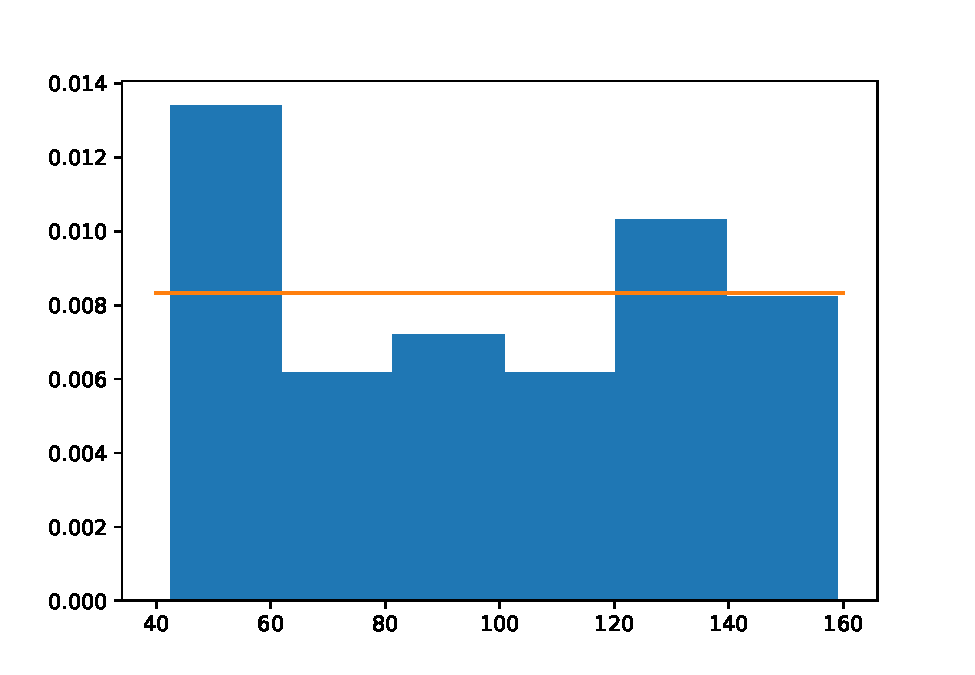
\includegraphics{_main_files/figure-latex/unnamed-chunk-209-11.pdf}

Ami az \texttt{rvs} függvények további nagy előnye, hogy ha kihasználjuk a függvény \texttt{random\_state} paraméterét, és \textbf{mindannyian beírjuk oda ugyan azt a számot}, pl. mondjuk az én szülinapom évét, ami \(1992\), akkor \textbf{mindenki ugyan azt az \(50\) db véletlen számot generálta le!} És ugyan azt a hisztogramot fogjuk már bambulni!:)

\begin{Shaded}
\begin{Highlighting}[]
\CommentTok{\# U(40,160) minta generálása}
\NormalTok{SzerencsésebbVéletlenek }\OperatorTok{=}\NormalTok{ stats.uniform.rvs(}
\NormalTok{  loc }\OperatorTok{=}\NormalTok{ eloszlás\_alsó\_határ,}
\NormalTok{  scale }\OperatorTok{=}\NormalTok{ eloszlás\_terjedelem,}
\NormalTok{  size }\OperatorTok{=} \DecValTok{50}\NormalTok{,}
\NormalTok{  random\_state }\OperatorTok{=} \DecValTok{1992}\NormalTok{)}

\CommentTok{\# Eredmény ellenőrzése hisztogramon}
\NormalTok{Hisztogram }\OperatorTok{=}\NormalTok{ plt.hist(SzerencsésebbVéletlenek, bins }\OperatorTok{=} \DecValTok{6}\NormalTok{, density }\OperatorTok{=} \VariableTok{True}\NormalTok{)}
\NormalTok{x\_tengely }\OperatorTok{=}\NormalTok{ np.arange(eloszlás\_alsó\_határ, eloszlás\_felső\_határ, }\FloatTok{0.01}\NormalTok{)}
\NormalTok{y\_tengely }\OperatorTok{=}\NormalTok{ stats.uniform.pdf(x }\OperatorTok{=}\NormalTok{ x\_tengely, loc }\OperatorTok{=}\NormalTok{ eloszlás\_alsó\_határ,scale }\OperatorTok{=}\NormalTok{ eloszlás\_terjedelem)}
\NormalTok{plt.plot(x\_tengely, y\_tengely)}
\NormalTok{plt.show()}
\end{Highlighting}
\end{Shaded}

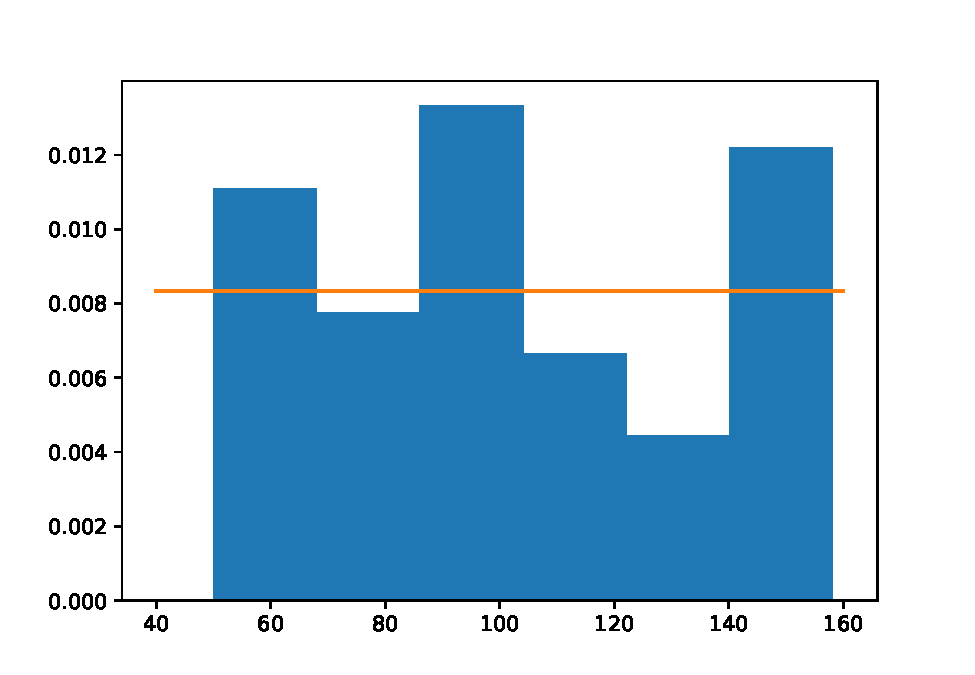
\includegraphics{_main_files/figure-latex/unnamed-chunk-210-13.pdf}

Pazar! :) A \texttt{random\_state} paraméterben megadott \(1992\) értéket szokás a véletlenszám generálás \textbf{véletlen magjának} nevezni. In English \emph{random seed}.

Generáljunk még az \(U(40, 160)\) eloszlás \(50\) elemű mintája mellé egy \(50\) elemű \(N(80,20)\) és egy \(50\) elemű \(Exp(0.0125)\) eloszlású mintát is, szintén \(1992\)-es véletlen maggal. Majd fűzzük össze az eredményeket egy \texttt{pandas} data frame-be úgy, hogy a különböző eloszlású adatok adják a tábla oszlopait (sorok száma akkor így 50 lesz ugyebár).
Az Exponenciális eloszlás \(\lambda\) paramétert a \texttt{scipy} függvények \texttt{scale} paraméterében lehet megadni a reciprokával. Hiszen az Exponenciális eloszlás szórása \(\frac{1}{\lambda}\). Emlékezetetőnek lásd 1. heti tananyag 3. fejezet!

\begin{Shaded}
\begin{Highlighting}[]
\CommentTok{\# N(80,20) minta generálása}
\NormalTok{átlag }\OperatorTok{=} \DecValTok{80}
\NormalTok{szórás }\OperatorTok{=} \DecValTok{20}

\NormalTok{NormalisAdatok }\OperatorTok{=}\NormalTok{ stats.norm.rvs(}
\NormalTok{  loc }\OperatorTok{=}\NormalTok{ átlag,}
\NormalTok{  scale }\OperatorTok{=}\NormalTok{ szórás,}
\NormalTok{  size }\OperatorTok{=} \DecValTok{50}\NormalTok{,}
\NormalTok{  random\_state }\OperatorTok{=} \DecValTok{1992}\NormalTok{)}
  
\CommentTok{\# Exp(0.0125) minta generálása}
\NormalTok{lam }\OperatorTok{=} \FloatTok{0.0125}

\NormalTok{ExpiAdatok }\OperatorTok{=}\NormalTok{ stats.expon.rvs(}
\NormalTok{  scale }\OperatorTok{=}\NormalTok{ (}\DecValTok{1}\OperatorTok{/}\NormalTok{lam),}
\NormalTok{  size }\OperatorTok{=} \DecValTok{50}\NormalTok{,}
\NormalTok{  random\_state }\OperatorTok{=} \DecValTok{1992}\NormalTok{)}

\CommentTok{\# Eredmények összefüzése data frame{-}be}
\ImportTok{import}\NormalTok{ pandas }\ImportTok{as}\NormalTok{ pd}

\NormalTok{AdatokEgyben }\OperatorTok{=}\NormalTok{ pd.DataFrame(}
  \BuiltInTok{list}\NormalTok{(}\BuiltInTok{zip}\NormalTok{(SzerencsésebbVéletlenek, NormalisAdatok, ExpiAdatok)),}
\NormalTok{  columns}\OperatorTok{=}\NormalTok{[}\StringTok{\textquotesingle{}Egyenletes\textquotesingle{}}\NormalTok{,}\StringTok{\textquotesingle{}Normal\textquotesingle{}}\NormalTok{, }\StringTok{\textquotesingle{}Expon\textquotesingle{}}\NormalTok{])}
\NormalTok{AdatokEgyben.info()}
\end{Highlighting}
\end{Shaded}

\begin{verbatim}
## <class 'pandas.core.frame.DataFrame'>
## RangeIndex: 50 entries, 0 to 49
## Data columns (total 3 columns):
##  #   Column      Non-Null Count  Dtype  
## ---  ------      --------------  -----  
##  0   Egyenletes  50 non-null     float64
##  1   Normal      50 non-null     float64
##  2   Expon       50 non-null     float64
## dtypes: float64(3)
## memory usage: 1.3 KB
\end{verbatim}

Szuper, az \texttt{info} metódus alapján megvan egyben a \(3\) db \(50\) elemű mintánk! Egy-egy \(k=6\) osztályközzel operáló hisztogramon meg is tudjuk nézni az eredményt, hála a data frame \texttt{hist} metódusának. :)

\begin{Shaded}
\begin{Highlighting}[]
\NormalTok{AdatokEgyben.hist(bins }\OperatorTok{=} \DecValTok{6}\NormalTok{)}
\end{Highlighting}
\end{Shaded}

\begin{verbatim}
## array([[<Axes: title={'center': 'Egyenletes'}>,
##         <Axes: title={'center': 'Normal'}>],
##        [<Axes: title={'center': 'Expon'}>, <Axes: >]], dtype=object)
\end{verbatim}

\begin{Shaded}
\begin{Highlighting}[]
\NormalTok{plt.show()}
\end{Highlighting}
\end{Shaded}

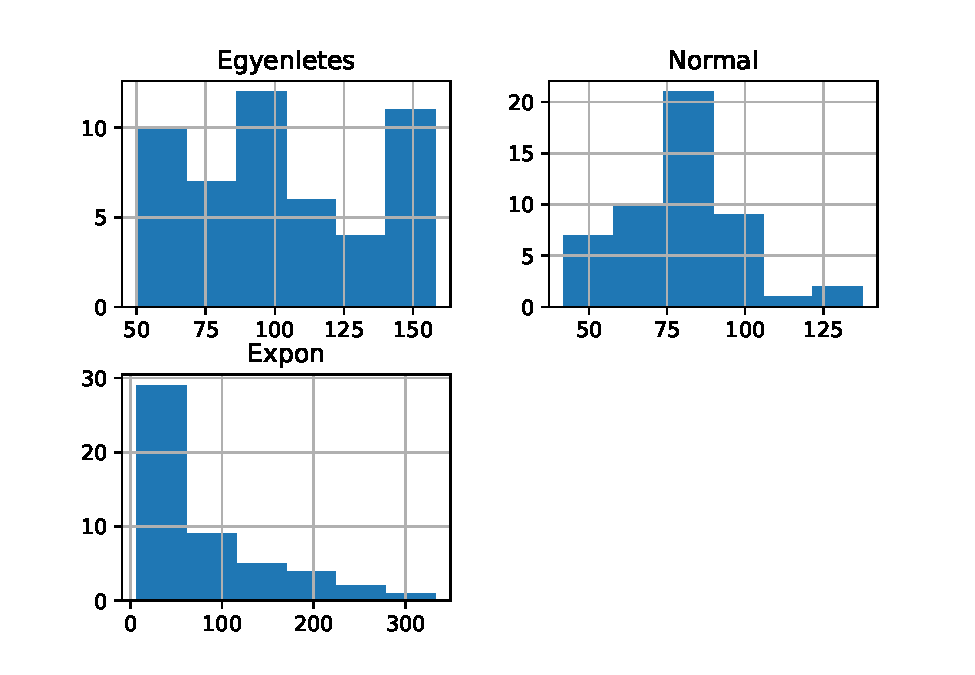
\includegraphics{_main_files/figure-latex/unnamed-chunk-212-15.pdf}

Na, meg is vagyunk, nagyjából mindegyik hisztogram követi a neki megfelelő Egyenletes, Normális és Exponenciális sűrűségfüggvény alakot.

\section{Elvi Eloszlás vs Megfigyelt Minta}\label{elvi-eloszluxe1s-vs-megfigyelt-minta}

Azt már több soron megállapítottuk, hogy a \textbf{megfigyelt adatokból készített hisztogramok NEM követik hajszálpontosan a hozzájuk tartozó eloszlások sűrűségfüggvényeit}. Valamennyire eltérnek tőle, ezt az előző fejezet végén álló 3 hisztogram is szemlélteti.
Ez amúgy egy \textbf{teljesen logikus és természetes jelenség}, hiszen az általunk vizsgált eloszlások \(f(x)\) sűrűségfüggvényei rengeteg számhoz rendelnek pozitív bekövetkezési valószínűséget egy véletlen húzás esetén:

\begin{itemize}
\tightlist
\item
  Az \(N(80,20)\) eloszlás konkrétan \emph{minden valós számnak} pozitív bekövetkezési esélyt tulajdonít
\item
  Az \(Exp(0.0125)\) eloszlás \emph{minden pozitív valós számnak}
\item
  Az \(U(40,160)\) pedig \emph{minden \(40\) és \(160\) közötti valós számnak}
\end{itemize}

Mindegyik számhalmaz elemszáma \textbf{végtelen}. Tehát, \textbf{akármelyik eloszlást is nézzük}, ahhoz hogy a \textbf{sűrűségfüggvényt teljes egészében meg tudjuk figyelni, végtelen sok elemű mintákat kéne generálni}. Nyilván, ez nem nagyon fog sosem összejönni. Ezért vannak a \textbf{némileg hektikus hisztogram alakok}. :)

Ami csak azért zavaró, mert a \textbf{valóságban nem vagyunk istenségek}, így a megfigyelt mintánk mögött meghúzódó \textbf{valódi sűrűségfüggvényt SOSEM tudjuk megfigyelni}, csak azokat az \textbf{adatokat, amiket a mintánk tartalmaz}. A minta elemszáma pedig sosem végtelen. \textbf{Legfeljebb csak reménykedni tudunk abban, hogy a minta hisztogram alapján sac/kb be tudjuk lőni, hogy az adataink mögött milyen eloszlás lappang a háttérben}.
Ugyan ez \textbf{igaz a különféle statisztikai mutatókra} is! Értelemszerűen \textbf{más értékeket kapunk az átlagra, szórásra, mediánra vagy az \(x\)-nél kisebb elemek arányára, ha azokat a megfigyelt mintaadatokból számítjuk, és nem az adatok mögöt rejtőző sűrűségfüggvény alapján}!

\subsection{Az elvi eloszlás alapján számolt statisztikai mutatók}\label{az-elvi-eloszluxe1s-alapjuxe1n-szuxe1molt-statisztikai-mutatuxf3k}

Vegyük csak végig, hogy a \textbf{3 vizsgált eloszlásunkban} hogyan is kapjuk meg a \textbf{sűrűségfüggvény ismeretében az alap statisztikai mutatókat}.

\begin{itemize}
\tightlist
\item
  \(N(80,20)\) eloszlás

  \begin{itemize}
  \tightlist
  \item
    Átlag: \(\mu=80\)
  \item
    Szórás: \(\sigma=20\)
  \item
    Medián: inverz függvény (\texttt{ppf}) értéke \(0.5\)-nél
  \item
    100-nál kisebb értékek aránya: \(P(Y_i<100)=\int_{-\infty}^{100}{f(x)}dx\)
  \end{itemize}
\item
  \(Exp(0.0125)\) eloszlás

  \begin{itemize}
  \tightlist
  \item
    Átlag: \(\mu=\frac{1}{\lambda}=\frac{1}{0.0125}=80\)
  \item
    Szórás: \(\sigma=\frac{1}{\lambda}=\frac{1}{0.0125}=80\)
  \item
    Medián: inverz függvény (\texttt{ppf}) értéke \(0.5\)-nél
  \item
    100-nál kisebb értékek aránya: \(P(Y_i<100)=\int_{-\infty}^{100}{f(x)}dx\)
  \end{itemize}
\item
  \(U(40,160)\) eloszlás

  \begin{itemize}
  \tightlist
  \item
    Átlag: \(\mu=\frac{a+b}{2}=\frac{40+160}{2}=100\)
  \item
    Szórás: \(\sigma=\frac{b-a}{\sqrt{12}}=\frac{160-40}{\sqrt{12}}=34.64\)
  \item
    Medián: inverz függvény (\texttt{ppf}) értéke \(0.5\)-nél
  \item
    100-nál kisebb értékek aránya: \(P(Y_i<100)=\int_{-\infty}^{100}{f(x)}dx\)
  \end{itemize}
\end{itemize}

Ezeket \textbf{számoljuk is ki minden eloszlásra} egy-egy külön \texttt{list}-be, majd fűzzük őket össze egy data frame-be! A data frame sorindexeit pedig nevezzük el a számított mutatók neve alapján!

\begin{Shaded}
\begin{Highlighting}[]
\CommentTok{\# N(80,20) paraméterek}
\NormalTok{átlag }\OperatorTok{=} \DecValTok{80}
\NormalTok{szórás }\OperatorTok{=} \DecValTok{20}

\CommentTok{\# Exp(0.0125) paraméterek}
\NormalTok{lam }\OperatorTok{=} \FloatTok{0.0125}

\CommentTok{\# U(40,160) paraméterek}
\NormalTok{eloszlás\_alsó\_határ }\OperatorTok{=} \DecValTok{40}
\NormalTok{eloszlás\_felső\_határ }\OperatorTok{=} \DecValTok{160}
\NormalTok{eloszlás\_terjedelem }\OperatorTok{=}\NormalTok{ eloszlás\_felső\_határ }\OperatorTok{{-}}\NormalTok{ eloszlás\_alsó\_határ}

\NormalTok{NormalisStat }\OperatorTok{=}\NormalTok{ [}
\NormalTok{  átlag, }\CommentTok{\# Átlag}
\NormalTok{  szórás, }\CommentTok{\# Szórás}
\NormalTok{  stats.norm.ppf(}\FloatTok{0.5}\NormalTok{, loc}\OperatorTok{=}\NormalTok{átlag, scale}\OperatorTok{=}\NormalTok{szórás), }\CommentTok{\# Medián}
\NormalTok{  stats.norm.cdf(}\DecValTok{100}\NormalTok{, loc}\OperatorTok{=}\NormalTok{átlag, scale}\OperatorTok{=}\NormalTok{szórás)] }\CommentTok{\# P(Y\_i\textless{}100)}

\NormalTok{ExponStat }\OperatorTok{=}\NormalTok{ [}
\NormalTok{  (}\DecValTok{1}\OperatorTok{/}\NormalTok{lam), }\CommentTok{\# Átlag}
\NormalTok{  (}\DecValTok{1}\OperatorTok{/}\NormalTok{lam), }\CommentTok{\# Szórás}
\NormalTok{  stats.expon.ppf(}\FloatTok{0.5}\NormalTok{, scale}\OperatorTok{=}\NormalTok{(}\DecValTok{1}\OperatorTok{/}\NormalTok{lam)), }\CommentTok{\# Medián}
\NormalTok{  stats.expon.cdf(}\DecValTok{100}\NormalTok{, scale}\OperatorTok{=}\NormalTok{(}\DecValTok{1}\OperatorTok{/}\NormalTok{lam))] }\CommentTok{\# P(Y\_i\textless{}100)}

\NormalTok{EgyenletesStat }\OperatorTok{=}\NormalTok{ [}
\NormalTok{  ((eloszlás\_alsó\_határ }\OperatorTok{+}\NormalTok{ eloszlás\_felső\_határ)}\OperatorTok{/}\DecValTok{2}\NormalTok{), }\CommentTok{\# Átlag}
\NormalTok{  ((eloszlás\_felső\_határ}\OperatorTok{{-}}\NormalTok{eloszlás\_alsó\_határ)}\OperatorTok{/}\NormalTok{np.sqrt(}\DecValTok{12}\NormalTok{)), }\CommentTok{\# Szórás}
\NormalTok{  stats.uniform.ppf(}\FloatTok{0.5}\NormalTok{, loc}\OperatorTok{=}\NormalTok{eloszlás\_alsó\_határ, scale}\OperatorTok{=}\NormalTok{eloszlás\_terjedelem), }\CommentTok{\# Medián}
\NormalTok{  stats.uniform.cdf(}\DecValTok{100}\NormalTok{, loc}\OperatorTok{=}\NormalTok{eloszlás\_alsó\_határ, scale}\OperatorTok{=}\NormalTok{eloszlás\_terjedelem)] }\CommentTok{\# P(Y\_i\textless{}100)}

\NormalTok{ElviStatMutatok }\OperatorTok{=}\NormalTok{ pd.DataFrame(}
  \BuiltInTok{list}\NormalTok{(}\BuiltInTok{zip}\NormalTok{(EgyenletesStat, NormalisStat, ExponStat)),}
\NormalTok{  columns}\OperatorTok{=}\NormalTok{[}\StringTok{\textquotesingle{}Egyenletes\textquotesingle{}}\NormalTok{,}\StringTok{\textquotesingle{}Normal\textquotesingle{}}\NormalTok{, }\StringTok{\textquotesingle{}Expon\textquotesingle{}}\NormalTok{],}
\NormalTok{  index }\OperatorTok{=}\NormalTok{ [}\StringTok{\textquotesingle{}Atlag\textquotesingle{}}\NormalTok{, }\StringTok{\textquotesingle{}Szoras\textquotesingle{}}\NormalTok{, }\StringTok{\textquotesingle{}Median\textquotesingle{}}\NormalTok{, }\StringTok{\textquotesingle{}P(Y\_i\textless{}100)\textquotesingle{}}\NormalTok{]}
\NormalTok{)}

\NormalTok{ElviStatMutatok}
\end{Highlighting}
\end{Shaded}

\begin{verbatim}
##             Egyenletes     Normal      Expon
## Atlag       100.000000  80.000000  80.000000
## Szoras       34.641016  20.000000  80.000000
## Median      100.000000  80.000000  55.451774
## P(Y_i<100)    0.500000   0.841345   0.713495
\end{verbatim}

Meg is vagyunk!

\subsection{A megfigyelt minta alapján számolt statisztikai mutatók}\label{a-megfigyelt-minta-alapjuxe1n-szuxe1molt-statisztikai-mutatuxf3k}

Most pedig \textbf{tegyük az elvi statisztikai mutatók értéke mellé az \(50\) elemű mintákból számolt verzióikat!} Hasonlóan összerakhatjuk őket egy data frame-be, mint fentebb csináltuk az elvi értékekkel.

A \(100\)-nál kisebb értékek arányának (relatív gyakoriságának) számolásához két technikai megjegyzés:

\begin{itemize}
\tightlist
\item
  A számolásnál azt a trükköt sütjük el, hogy pl. az \texttt{AdatokEgyben{[}\textquotesingle{}Normal\textquotesingle{}{]}\ \textless{}\ 100} parancs egy \texttt{bool} tömböt ad vissza aszerint, hogy az \texttt{AdatokEgyben{[}\textquotesingle{}Normal\textquotesingle{}{]}\ \textless{}\ 100} logikai állítás kire \texttt{True} és \texttt{False}.
\item
  A \texttt{numpy} csomag \texttt{sum} függvénye pedig egy ilyen tömbre \texttt{True\ =\ 1} és \texttt{False\ =\ 0} kódolásokkal végzi el az összegzést: azaz megadja a \emph{kedvező esetek}, a 100-nál kisebb értékek \emph{darabszámát}.
\end{itemize}

\begin{Shaded}
\begin{Highlighting}[]
\NormalTok{NormalisMintaStat }\OperatorTok{=}\NormalTok{ [}
\NormalTok{  np.mean(AdatokEgyben[}\StringTok{\textquotesingle{}Normal\textquotesingle{}}\NormalTok{]), }\CommentTok{\# Átlag}
\NormalTok{  np.std(AdatokEgyben[}\StringTok{\textquotesingle{}Normal\textquotesingle{}}\NormalTok{]), }\CommentTok{\# Szórás}
\NormalTok{  np.median(AdatokEgyben[}\StringTok{\textquotesingle{}Normal\textquotesingle{}}\NormalTok{]), }\CommentTok{\# Medián}
\NormalTok{  np.}\BuiltInTok{sum}\NormalTok{(AdatokEgyben[}\StringTok{\textquotesingle{}Normal\textquotesingle{}}\NormalTok{] }\OperatorTok{\textless{}} \DecValTok{100}\NormalTok{)}\OperatorTok{/}\BuiltInTok{len}\NormalTok{(AdatokEgyben)] }\CommentTok{\# P(Y\_i\textless{}100), most relatív gyak.}

\NormalTok{ExponMintaStat }\OperatorTok{=}\NormalTok{ [}
\NormalTok{  np.mean(AdatokEgyben[}\StringTok{\textquotesingle{}Expon\textquotesingle{}}\NormalTok{]), }\CommentTok{\# Átlag}
\NormalTok{  np.std(AdatokEgyben[}\StringTok{\textquotesingle{}Expon\textquotesingle{}}\NormalTok{]), }\CommentTok{\# Szórás}
\NormalTok{  np.median(AdatokEgyben[}\StringTok{\textquotesingle{}Expon\textquotesingle{}}\NormalTok{]), }\CommentTok{\# Medián}
\NormalTok{  np.}\BuiltInTok{sum}\NormalTok{(AdatokEgyben[}\StringTok{\textquotesingle{}Expon\textquotesingle{}}\NormalTok{] }\OperatorTok{\textless{}} \DecValTok{100}\NormalTok{)}\OperatorTok{/}\BuiltInTok{len}\NormalTok{(AdatokEgyben)] }\CommentTok{\# P(Y\_i\textless{}100), most relatív gyak.}

\NormalTok{EgyenletesMintaStat }\OperatorTok{=}\NormalTok{ [}
\NormalTok{  np.mean(AdatokEgyben[}\StringTok{\textquotesingle{}Egyenletes\textquotesingle{}}\NormalTok{]), }\CommentTok{\# Átlag}
\NormalTok{  np.std(AdatokEgyben[}\StringTok{\textquotesingle{}Egyenletes\textquotesingle{}}\NormalTok{]), }\CommentTok{\# Szórás}
\NormalTok{  np.median(AdatokEgyben[}\StringTok{\textquotesingle{}Egyenletes\textquotesingle{}}\NormalTok{]), }\CommentTok{\# Medián}
\NormalTok{  np.}\BuiltInTok{sum}\NormalTok{(AdatokEgyben[}\StringTok{\textquotesingle{}Egyenletes\textquotesingle{}}\NormalTok{] }\OperatorTok{\textless{}} \DecValTok{100}\NormalTok{)}\OperatorTok{/}\BuiltInTok{len}\NormalTok{(AdatokEgyben)] }\CommentTok{\# P(Y\_i\textless{}100), most relatív gyak.}

\NormalTok{MintaStatMutatok }\OperatorTok{=}\NormalTok{ pd.DataFrame(}
  \BuiltInTok{list}\NormalTok{(}\BuiltInTok{zip}\NormalTok{(EgyenletesMintaStat, NormalisMintaStat, ExponMintaStat)),}
\NormalTok{  columns}\OperatorTok{=}\NormalTok{[}\StringTok{\textquotesingle{}Egyenletes\textquotesingle{}}\NormalTok{,}\StringTok{\textquotesingle{}Normal\textquotesingle{}}\NormalTok{, }\StringTok{\textquotesingle{}Expon\textquotesingle{}}\NormalTok{],}
\NormalTok{  index }\OperatorTok{=}\NormalTok{ [}\StringTok{\textquotesingle{}Atlag\textquotesingle{}}\NormalTok{, }\StringTok{\textquotesingle{}Szoras\textquotesingle{}}\NormalTok{, }\StringTok{\textquotesingle{}Median\textquotesingle{}}\NormalTok{, }\StringTok{\textquotesingle{}P(Y\_i\textless{}100)\textquotesingle{}}\NormalTok{]}
\NormalTok{)}

\NormalTok{MintaStatMutatok}
\end{Highlighting}
\end{Shaded}

\begin{verbatim}
##             Egyenletes     Normal      Expon
## Atlag       101.865225  78.951917  82.311381
## Szoras       33.462534  18.922748  76.278763
## Median       97.446914  76.384652  52.148485
## P(Y_i<100)    0.540000   0.880000   0.700000
\end{verbatim}

Meg is vagyunk!

\subsection{A mintavételi hiba (MVH) koncepciója}\label{a-mintavuxe9teli-hiba-mvh-koncepciuxf3ja}

Nézzük össze akkor kétféle stat. mutatókat tartalmazó data frame-et egymással!

\begin{Shaded}
\begin{Highlighting}[]
\NormalTok{ElviStatMutatok}
\end{Highlighting}
\end{Shaded}

\begin{verbatim}
##             Egyenletes     Normal      Expon
## Atlag       100.000000  80.000000  80.000000
## Szoras       34.641016  20.000000  80.000000
## Median      100.000000  80.000000  55.451774
## P(Y_i<100)    0.500000   0.841345   0.713495
\end{verbatim}

\begin{Shaded}
\begin{Highlighting}[]
\NormalTok{MintaStatMutatok}
\end{Highlighting}
\end{Shaded}

\begin{verbatim}
##             Egyenletes     Normal      Expon
## Atlag       101.865225  78.951917  82.311381
## Szoras       33.462534  18.922748  76.278763
## Median       97.446914  76.384652  52.148485
## P(Y_i<100)    0.540000   0.880000   0.700000
\end{verbatim}

Láthatjuk, hogy a \textbf{statisztikai mutatók terén is azt tapasztaljuk, amit a hisztogramok és a sűrűségfüggvény esetén}. Az \textbf{elvi értékekhez az \(50\) elemű mintából számolt mutatók közel vannak, de nem egyeznek velük}.

A \textbf{kétféle értékek (elvi és mintából számolt) közti eltérést hívjuk MINTAVÉTELI HIBÁNAK (MVH)}. Mivel a gyakorlatban \textbf{csak egy adott elemszámú mintát tudunk megfigyelni}, és abból kellene rájönnünk a vizsgált mutatók valódi értékére, a hisztogramból meg a valódi eloszlásra, \textbf{nagyon jó lenne ezt az MVH-t megmérni/kiszámolni/megbecsülni}! Na, ez a \textbf{statisztikai becsléselmélet alapfeladata}!

Az MVH kiszámolásához hosszú az út, de az \textbf{MVH viselekdését megérthetjük, ha generálunk még pár extra mintát az eddig vizsgált eloszlásokból, különböző elemszámokkal}.

Ehhez írjunk egy Python függvényt, ami az eddig elvégzett műveleteinket egy függvényben valószítja meg tetszőleges mintaelemszám és véletlenmag mellett:

\begin{itemize}
\tightlist
\item
  \(N(80,20)\), \(Exp(0.0125)\) és \(U(40,160)\) eloszlású minták generálása
\item
  A mintákból a vizsgált 4 statisztikai mutató számítása és azok összefüzése data frame-be
\end{itemize}

Ez a függvény némi copy-paste után az alábbi formát ölti.

\begin{Shaded}
\begin{Highlighting}[]
\KeywordTok{def}\NormalTok{ MintaGeneralas(Elemszam, VeletlenMag):}
    \CommentTok{\# U(40, 160) minta generálása}
\NormalTok{    eloszlás\_alsó\_határ }\OperatorTok{=} \DecValTok{40}
\NormalTok{    eloszlás\_terjedelem }\OperatorTok{=} \DecValTok{160}\OperatorTok{{-}}\DecValTok{40}
  
\NormalTok{    SzerencsésebbVéletlenek }\OperatorTok{=}\NormalTok{ stats.uniform.rvs(}
\NormalTok{      loc }\OperatorTok{=}\NormalTok{ eloszlás\_alsó\_határ,}
\NormalTok{      scale }\OperatorTok{=}\NormalTok{ eloszlás\_terjedelem,}
\NormalTok{      size }\OperatorTok{=}\NormalTok{ Elemszam,}
\NormalTok{      random\_state }\OperatorTok{=}\NormalTok{ VeletlenMag)}
  
    \CommentTok{\# N(80,20) minta generálása}
\NormalTok{    átlag }\OperatorTok{=} \DecValTok{80}
\NormalTok{    szórás }\OperatorTok{=} \DecValTok{20}

\NormalTok{    NormalisAdatok }\OperatorTok{=}\NormalTok{ stats.norm.rvs(}
\NormalTok{      loc }\OperatorTok{=}\NormalTok{ átlag,}
\NormalTok{      scale }\OperatorTok{=}\NormalTok{ szórás,}
\NormalTok{      size }\OperatorTok{=}\NormalTok{ Elemszam,}
\NormalTok{      random\_state }\OperatorTok{=}\NormalTok{ VeletlenMag)}
  
    \CommentTok{\# Exp(0.0125) minta generálása}
\NormalTok{    lam }\OperatorTok{=} \FloatTok{0.0125}

\NormalTok{    ExpiAdatok }\OperatorTok{=}\NormalTok{ stats.expon.rvs(}
\NormalTok{      scale }\OperatorTok{=}\NormalTok{ (}\DecValTok{1}\OperatorTok{/}\NormalTok{lam),}
\NormalTok{      size }\OperatorTok{=}\NormalTok{ Elemszam,}
\NormalTok{      random\_state }\OperatorTok{=}\NormalTok{ VeletlenMag)}

    \CommentTok{\# Eredmények összefüzése data frame{-}be}
\NormalTok{    AdatokEgyben }\OperatorTok{=}\NormalTok{ pd.DataFrame(}
      \BuiltInTok{list}\NormalTok{(}\BuiltInTok{zip}\NormalTok{(SzerencsésebbVéletlenek, NormalisAdatok, ExpiAdatok)),}
\NormalTok{      columns}\OperatorTok{=}\NormalTok{[}\StringTok{\textquotesingle{}Egyenletes\textquotesingle{}}\NormalTok{,}\StringTok{\textquotesingle{}Normal\textquotesingle{}}\NormalTok{, }\StringTok{\textquotesingle{}Expon\textquotesingle{}}\NormalTok{])}

\NormalTok{    NormalisMintaStat }\OperatorTok{=}\NormalTok{ [}
\NormalTok{      np.mean(AdatokEgyben[}\StringTok{\textquotesingle{}Normal\textquotesingle{}}\NormalTok{]), }\CommentTok{\# Átlag}
\NormalTok{      np.std(AdatokEgyben[}\StringTok{\textquotesingle{}Normal\textquotesingle{}}\NormalTok{]), }\CommentTok{\# Szórás}
\NormalTok{      np.median(AdatokEgyben[}\StringTok{\textquotesingle{}Normal\textquotesingle{}}\NormalTok{]), }\CommentTok{\# Medián}
\NormalTok{      np.}\BuiltInTok{sum}\NormalTok{(AdatokEgyben[}\StringTok{\textquotesingle{}Normal\textquotesingle{}}\NormalTok{] }\OperatorTok{\textless{}} \DecValTok{100}\NormalTok{)}\OperatorTok{/}\BuiltInTok{len}\NormalTok{(AdatokEgyben)] }\CommentTok{\# P(Y\_i\textless{}100), most relatív gyak.}

\NormalTok{    ExponMintaStat }\OperatorTok{=}\NormalTok{ [}
\NormalTok{      np.mean(AdatokEgyben[}\StringTok{\textquotesingle{}Expon\textquotesingle{}}\NormalTok{]), }\CommentTok{\# Átlag}
\NormalTok{      np.std(AdatokEgyben[}\StringTok{\textquotesingle{}Expon\textquotesingle{}}\NormalTok{]), }\CommentTok{\# Szórás}
\NormalTok{      np.median(AdatokEgyben[}\StringTok{\textquotesingle{}Expon\textquotesingle{}}\NormalTok{]), }\CommentTok{\# Medián}
\NormalTok{      np.}\BuiltInTok{sum}\NormalTok{(AdatokEgyben[}\StringTok{\textquotesingle{}Expon\textquotesingle{}}\NormalTok{] }\OperatorTok{\textless{}} \DecValTok{100}\NormalTok{)}\OperatorTok{/}\BuiltInTok{len}\NormalTok{(AdatokEgyben)] }\CommentTok{\# P(Y\_i\textless{}100), most relatív gyak.}

\NormalTok{    EgyenletesMintaStat }\OperatorTok{=}\NormalTok{ [}
\NormalTok{      np.mean(AdatokEgyben[}\StringTok{\textquotesingle{}Egyenletes\textquotesingle{}}\NormalTok{]), }\CommentTok{\# Átlag}
\NormalTok{      np.std(AdatokEgyben[}\StringTok{\textquotesingle{}Egyenletes\textquotesingle{}}\NormalTok{]), }\CommentTok{\# Szórás}
\NormalTok{      np.median(AdatokEgyben[}\StringTok{\textquotesingle{}Egyenletes\textquotesingle{}}\NormalTok{]), }\CommentTok{\# Medián}
\NormalTok{      np.}\BuiltInTok{sum}\NormalTok{(AdatokEgyben[}\StringTok{\textquotesingle{}Egyenletes\textquotesingle{}}\NormalTok{] }\OperatorTok{\textless{}} \DecValTok{100}\NormalTok{)}\OperatorTok{/}\BuiltInTok{len}\NormalTok{(AdatokEgyben)] }\CommentTok{\# P(Y\_i\textless{}100), most relatív gyak.}

\NormalTok{    MintaStatMutatok }\OperatorTok{=}\NormalTok{ pd.DataFrame(}
      \BuiltInTok{list}\NormalTok{(}\BuiltInTok{zip}\NormalTok{(EgyenletesMintaStat, NormalisMintaStat, ExponMintaStat)),}
\NormalTok{      columns}\OperatorTok{=}\NormalTok{[}\StringTok{\textquotesingle{}Egyenletes\textquotesingle{}}\NormalTok{,}\StringTok{\textquotesingle{}Normal\textquotesingle{}}\NormalTok{, }\StringTok{\textquotesingle{}Expon\textquotesingle{}}\NormalTok{],}
\NormalTok{      index }\OperatorTok{=}\NormalTok{ [}\StringTok{\textquotesingle{}Atlag\textquotesingle{}}\NormalTok{, }\StringTok{\textquotesingle{}Szoras\textquotesingle{}}\NormalTok{, }\StringTok{\textquotesingle{}Median\textquotesingle{}}\NormalTok{, }\StringTok{\textquotesingle{}P(Y\_i\textless{}100)\textquotesingle{}}\NormalTok{]}
\NormalTok{    )}
    
    \ControlFlowTok{return}\NormalTok{ MintaStatMutatok}
\end{Highlighting}
\end{Shaded}

Ha a \texttt{MintaGeneralas} függvény definícióját megadó fenti kód szépen lefutott, akkor a következőképpen tudjuk használni a függvényt egy \(50\) elemű minta generálására \(1994\)-es véletlenmag mellett.

\begin{Shaded}
\begin{Highlighting}[]
\NormalTok{MintaGeneralas(}\DecValTok{50}\NormalTok{, }\DecValTok{1994}\NormalTok{)}
\end{Highlighting}
\end{Shaded}

\begin{verbatim}
##             Egyenletes     Normal      Expon
## Atlag       104.663427  81.542000  86.208355
## Szoras       33.384088  23.684983  74.027139
## Median      107.564478  83.357606  66.232602
## P(Y_i<100)    0.400000   0.800000   0.720000
\end{verbatim}

Na, úgy néz ki működik! :)

Akkor most lessük meg \textbf{mi történik a mintából számolt és az elvi statisztikai mutatók közti különbségekkel} (alias az MVH-val), ha \textbf{nem \(50\), hanem mondjuk \(1000\) elemű mintákat generálok az eloszlásokból}.

\begin{Shaded}
\begin{Highlighting}[]
\NormalTok{ElviStatMutatok}
\end{Highlighting}
\end{Shaded}

\begin{verbatim}
##             Egyenletes     Normal      Expon
## Atlag       100.000000  80.000000  80.000000
## Szoras       34.641016  20.000000  80.000000
## Median      100.000000  80.000000  55.451774
## P(Y_i<100)    0.500000   0.841345   0.713495
\end{verbatim}

\begin{Shaded}
\begin{Highlighting}[]
\NormalTok{MintaGeneralas(}\DecValTok{50}\NormalTok{, }\DecValTok{1992}\NormalTok{)}
\end{Highlighting}
\end{Shaded}

\begin{verbatim}
##             Egyenletes     Normal      Expon
## Atlag       101.865225  78.951917  82.311381
## Szoras       33.462534  18.922748  76.278763
## Median       97.446914  76.384652  52.148485
## P(Y_i<100)    0.540000   0.880000   0.700000
\end{verbatim}

\begin{Shaded}
\begin{Highlighting}[]
\NormalTok{MintaGeneralas(}\DecValTok{1000}\NormalTok{, }\DecValTok{1992}\NormalTok{)}
\end{Highlighting}
\end{Shaded}

\begin{verbatim}
##             Egyenletes     Normal      Expon
## Atlag       100.646326  80.106832  81.413684
## Szoras       34.791814  20.003538  80.432945
## Median      100.488619  79.798321  56.105934
## P(Y_i<100)    0.499000   0.838000   0.706000
\end{verbatim}

Na, hát ha \(1000\) elemet tudtam megfigyelni az \(50\) helyett, akkor minden statisztikai mutatóm mintából számolt értéke lényegesen közelebb van a valós, elvi értékhez! Tehát, olybá tűnik, hogy \textbf{mintaelemszám növelésével az MVH lecsökken!} Ez egy nagyon fontos tulajdonság, ami \textbf{minden statisztikai mutató esetén általánosságban igaz marad!}
Mivel ez egy marha fontos dolog, így kaptok róla egy mémet is! \textbf{Égjen csak ez be az agyakba! ;)}


\includegraphics[width=0.4\textwidth,height=\textheight]{sample_size.jpg}

További kísérletezgetésre a mintavétel hibával kapcsolatban, nyugodtan lehet használni az alábbi kis interaktív felületet.

A felületet nyomogatva érdemes megfigyelni pár dolgot.

\begin{itemize}
\tightlist
\item
  A mintaelemszám növelésével a hisztogram alakja is közelebb kerül az adatok mögött álló eloszlás sűrűségfüggvényéhez. Tehát \textbf{elemszám növelésével a sűrűségfüggvény mintavételi hibája is csökken} úgymond.
\item
  Az \textbf{átlag és a 100-nál kisebb értékek aránya} általában \textbf{mindhárom eloszlásnál elég közel van a valós, elméleti értékéhez}.
\item
  Ellenben a \textbf{medián és szórás} értékek az \textbf{exponenciális eloszlás esetében aránylag többször is durván eltérnek a valós értéktől még nagyobb} (pl. 500 körüli) \textbf{elemszám esetén is}.
\end{itemize}

\section{Statisztikai sokaságok FAE mintavételezése}\label{statisztikai-sokasuxe1gok-fae-mintavuxe9telezuxe9se}

Amit az első két fejezetben műveltünk az az \textbf{elméleti eloszlások Független Azonos Eloszlású, leánykori nevén FAE mintavételezése}.

A FAE mintának ezek szerint két jellemzője van:

\begin{itemize}
\tightlist
\item
  \textbf{Független}: a \textbf{mintaelemek kihúzása véletlenszerű}, tehát az, hogy mit húztam mondjuk 3-nak \textbf{nem függ} attól mit húztam 1-nek és 2-nak.
\item
  \textbf{Azonos Eloszlású}: A minta minden eleme \textbf{ugyan abból az eloszlásból} (pl. \(N(80,20)\) vagy \(Exp(0.0125)\)) származik, nincs közben váltás arra nézve, hogy épp milyen eloszlásból húzzuk ki véletlenszerűen az értékeket.
\end{itemize}

Ezt a FAE mintavételt \textbf{valós statisztikai adatsorok, azaz sokaságok esetén is el lehet végezni}, nem csak elméleti eloszlások esetén.
Mondjuk meg akarom ismerni a kb. 4,5 millió magyar munkavállaló havi bruttó átlagkeresetét. Nyilván a NAV-nál megvan mind a 4,5 millió dolgos magyar \emph{en\_ber} kereseti adata tételesen (tehát ezek az értékek nem egy exponenciális eloszlással vannak megadva pl., hanem tételesen fel vannak sorolva egy táblában valahol), csak hát tudjuk mikor adják ki ezeket az adatokat bárkinek is. Ezért inkább azt csináljuk, hogy mondjuk a népességnyilvántartótól elkérjük a 4,5 millió magyar munkavállaló lakcímét, beöntjük a címeket tartalmazó cetliket egy kalapba, és becsukott szemmel, random húzunk 100 címet \emph{visszatevéssel}, azaz egy kihúzott címet visszateszünk mindig a kalapba, és nem rakjuk félre. Majd mind a 100 címre elmegyünk és megkérdezzük az emberek havi bruttó keresetét. Ezzel a \textbf{véletlen, visszatevéses mintavétellel a magyar munkavállalók sokaságából} valójában \textbf{FAE mintavételezést végeztünk}. Miért is?

\begin{enumerate}
\def\labelenumi{\arabic{enumi}.}
\tightlist
\item
  A \textbf{mintaelemek függetlenek}, hiszen ``\emph{becsukott szemmel}'', véletlenszerűen húztuk ki a minta elemeket.
\item
  Mivel \textbf{visszatevéses volt a mintavétel, így a kersetek eloszlása nem változott meg a mintavétel során}. Tehát végig ugyan azt az elméleti kereseteloszlást mintavételeztünk. Pont úgy, mint amikor mindig ugyan abból az elvi sűrűségfüggvényből generáltuk a mintaelemeket az eddig elvégzett mintavételeink során.
\end{enumerate}

Tehát, bízunk abban, hogy ami mondjuk a \textbf{mintából számolt átlagkereset és a teljes sokaság átlagekeresete között áll az ugyan az az MVH, mint amivel találkoztunk az eloszlások elvi átlaga és a belőlük generált minták tapasztalati átlaga esetében is!!}
Persze a gyakorlatban \textbf{nem mindig tudunk ilyen szép FAE mintavételt végezni}, mert

\begin{enumerate}
\def\labelenumi{\arabic{enumi}.}
\tightlist
\item
  \textbf{Nem tudunk visszatenni} elemeket. Ez a \textbf{kisebbik gond}. Hiszen, ha a \textbf{minta mérete a sokaság méretéhez képest nagyon kicsi} (pl. 100 főt választunk kis a 4,5 millióból és nem 2 milliót :)), akkor a \textbf{visszatevéses és visszatevés nélküli mintavétel nagyjából ugyan az}, mert nagyon kicsi lesz az esélye annak, hogy a visszatevéses esetben valakit tényleg kétszer beválasztunk a mintába.
\item
  \textbf{Nem tudunk ténylegesen véletlenszerűen kiválasztani elemeket}. Ez a \textbf{nagyobb baj}. És sajnos gyakori is. Pl. \emph{nem kapunk címjegyzéket, amiből sorsolni lehet a mintánkba emberkéket}. Mert ekkor a mintavételi hiba mellé bejön az úgynevezett \textbf{nem mintavételi hiba}. Ezek olyan tényezők, amik ``\emph{emberi gyarlóság}'' miatt kerülnek a rendszerbe. Pl. nagyon tetszenek a vörös hajú lányok, így aránytalanul sokat kérdezek meg belőlük ahhoz képest ahányan a sokaságban vannak. Vagy, lusta vagyok lemenni 500 fő alatti településre, így az alacsonyabb keresetű társadalmi rétegből is kevesebb embert kérdezek meg, mint ahányat kéne a sokasági elemszámuk alapján. Tehát, szakszóval azt mondom, hogy a \textbf{minta nem lesz reprezentatív hajszínre és település méretre}. Ezekkel a \textbf{nem mintavételi hibákkal most nem foglalkozunk, feltesszük, hogy nincsenek}. Mert \textbf{kiszámolásuk és korrigálásuk elég bonyolult}, komplett mesterszakok foglalkoznak a kérdéssel.
\end{enumerate}

Szóval, első körben nézzük meg \textbf{hogyan tudunk Pythonban egy ismert sokaságból FAE mintát venni}. A LIDLBalaton2022.xlsx fájlban a 2022-es LIDL Balaton átúszás résztvevőinek \emph{neve, neme és percben mért időeredménye} található. Olvassuk be a táblát \texttt{pandas} data frame-be!

\begin{Shaded}
\begin{Highlighting}[]
\NormalTok{Balcsi }\OperatorTok{=}\NormalTok{ pd.read\_excel(}\StringTok{"LIDLBalaton2022.xlsx"}\NormalTok{)}

\NormalTok{Balcsi.info()}
\end{Highlighting}
\end{Shaded}

\begin{verbatim}
## <class 'pandas.core.frame.DataFrame'>
## RangeIndex: 9751 entries, 0 to 9750
## Data columns (total 3 columns):
##  #   Column  Non-Null Count  Dtype  
## ---  ------  --------------  -----  
##  0   Nev     9751 non-null   object 
##  1   Nem     9751 non-null   object 
##  2   PERC    9751 non-null   float64
## dtypes: float64(1), object(2)
## memory usage: 228.7+ KB
\end{verbatim}

\begin{Shaded}
\begin{Highlighting}[]
\NormalTok{Balcsi.head()}
\end{Highlighting}
\end{Shaded}

\begin{verbatim}
##                    Nev Nem        PERC
## 0           Aba Attila   F  142.416667
## 1        Abaffy Károly   F  197.883333
## 2        Abaffy Kornél   F  197.983333
## 3  Abelovszki Hajnalka   N  182.000000
## 4   Abért Valentin ifj   F  222.516667
\end{verbatim}

Szuper, úgy látszik megvan mind az \(N=9751\) versenyző időeredménye hiánytalanul. \textbf{Ez lesz most akkor a sokaságunk.}

Számoljunk ki az időeredményekre három statisztikai mutatót:

\begin{itemize}
\tightlist
\item
  Az \textbf{átlag}os időt Jele: \(\bar{Y}\) vagy \(\mu\)
\item
  Az egyéni idők \textbf{szórás}át Jele: \(\sigma\)
\item
  A 3 óra (180 perc) felett teljesítők \textbf{arányát} Jele: \(P\)

  \begin{itemize}
  \tightlist
  \item
    Itt a számolásnál azt a trükköt sütjük el, hogy a \texttt{Balcsi.PERC\ \textgreater{}\ 180} parancs egy \texttt{bool} tömböt ad vissza aszerint, hogy a \texttt{Balcsi.PERC\ \textgreater{}\ 180} logikai állítás kire \texttt{True} és \texttt{False}.
  \item
    A \texttt{numpy} csomag \texttt{sum} függvénye pedig egy ilyen tömbre \texttt{True\ =\ 1} és \texttt{False\ =\ 0} kódolásokkal végzi el az összegzést: azaz megadja a \emph{kedvező esetek}, a Balatont 180-an percnél hosszabb idő alatt átúszók \emph{darabszámát}.
  \end{itemize}
\end{itemize}

\begin{Shaded}
\begin{Highlighting}[]
\NormalTok{SokasagiAtlag }\OperatorTok{=}\NormalTok{ np.mean(Balcsi.PERC)}
\NormalTok{SokasagiSzoras }\OperatorTok{=}\NormalTok{ np.std(Balcsi.PERC)}
\NormalTok{SokasagiArany }\OperatorTok{=}\NormalTok{ np.}\BuiltInTok{sum}\NormalTok{(Balcsi.PERC }\OperatorTok{\textgreater{}} \DecValTok{180}\NormalTok{)}\OperatorTok{/}\BuiltInTok{len}\NormalTok{(Balcsi)}

\NormalTok{SokasagiAtlag}
\end{Highlighting}
\end{Shaded}

\begin{verbatim}
## 167.52914060096398
\end{verbatim}

\begin{Shaded}
\begin{Highlighting}[]
\NormalTok{SokasagiSzoras}
\end{Highlighting}
\end{Shaded}

\begin{verbatim}
## 44.08833385551663
\end{verbatim}

\begin{Shaded}
\begin{Highlighting}[]
\NormalTok{SokasagiArany}
\end{Highlighting}
\end{Shaded}

\begin{verbatim}
## 0.3295046661880833
\end{verbatim}

Meg is vagyunk, \textbf{ezek akkor a statisztikai mutatóink valós, sokasági értékei}:

\begin{itemize}
\tightlist
\item
  \(\bar{Y}=\mu=167.5\) perc
\item
  \(\sigma = 44.1\) perc
\item
  \(P = 0.3295=32.95\%\)
\end{itemize}

Ezek alapján a \textbf{sokaság, azaz a teljes adatsor esetén a következő jelölési konvenciókkal élünk}:

\begin{itemize}
\tightlist
\item
  Elemszám \(N\)
\item
  Sokaságból számított statisztikai mutatók együttes jelölése: \(\theta\)

  \begin{itemize}
  \tightlist
  \item
    Tehát \(\theta\) egy általános jelölés egy sokasági mutatószámra.
  \item
    Állhat mögötte átlag (\(\bar{Y}=\mu\)), szórás (\(\sigma\)), arány (\(P\)), de akár medián (\(Me\)), módusz (\(Mo\)) stb. is!
  \end{itemize}
\end{itemize}

Általános szabály, hogy a ``\emph{sokasági dolgokat}'' vagy \textbf{nagy} vagy \textbf{görög betűvel jelöljük}.

Akkor most \textbf{vegyünk a Balaton 2022-es átúszóinak a sokaságából} egy \(n=100\) elemű \textbf{mintát!} Szerencsére Pythonban ezt könnyű végrehajtani, mivel a \texttt{pandas} data frame-nek létezik \texttt{sample} metódusa, aminek az \texttt{n} paraméterében meg lehet mondani, hogy \textbf{hány elemű mintánk} legyen. A \texttt{replace\ =\ True} paraméter beállítással pedig azt mondjuk meg gépállatnak, hogy \textbf{visszatevéses véletlen, azaz FAE mintát} szeretnénk.
Itt is van \texttt{random\_state} paraméter, amit azonos számla (pl. továbbra is 1992-re) beállítva \emph{ugyan azt a véletlen mintát fogjuk kapni}.

\begin{Shaded}
\begin{Highlighting}[]
\NormalTok{BalcsiMinta }\OperatorTok{=}\NormalTok{ Balcsi.sample(n }\OperatorTok{=} \DecValTok{100}\NormalTok{, replace }\OperatorTok{=} \VariableTok{True}\NormalTok{, random\_state }\OperatorTok{=} \DecValTok{1992}\NormalTok{)}

\NormalTok{BalcsiMinta.info()}
\end{Highlighting}
\end{Shaded}

\begin{verbatim}
## <class 'pandas.core.frame.DataFrame'>
## Index: 100 entries, 7991 to 5727
## Data columns (total 3 columns):
##  #   Column  Non-Null Count  Dtype  
## ---  ------  --------------  -----  
##  0   Nev     100 non-null    object 
##  1   Nem     100 non-null    object 
##  2   PERC    100 non-null    float64
## dtypes: float64(1), object(2)
## memory usage: 3.1+ KB
\end{verbatim}

Olybá néz ki megvan az \(n=100\) elemű FAE mintánk! :)

Mielőtt nekiugrunk, és kiszámoljuk a minta alapján az időeredmények átlagát, szórását és a 3 órán felül úszók arányát, itt is szögezzünk le \textbf{jelölési konvenciót a mintára vonatkozóan}:

\begin{itemize}
\tightlist
\item
  Elemszám \(n\)
\item
  A mintából számított statisztikai mutatók együttes jelölése: \(\hat{\theta}\)

  \begin{itemize}
  \tightlist
  \item
    Tehát \(\hat{\theta}\) egy általános jelölés egy sokasági mutatószámra.
  \item
    Általánosságban a ``\emph{kalap}'', a \(\hat{}\) mindig a mintából \textbf{becsült} érték jele.
  \item
    Állhat \(\hat{\theta}\) mögött átlag (\(\bar{y}\)), szórás (\(s^*\)), arány (\(p\)), de akár medián (\(me\)), módusz (\(mo\)) stb. is!
  \end{itemize}
\end{itemize}

Általános szabály, hogy a ``\emph{mintából számolt dolgokat}'' vagy \textbf{kis betűvel} vagy \textbf{kalappal jelöljük}.

Na, akkor nézzük meg \textbf{a statisztikai mutatóink} \(n = 100\) elemű \textbf{mintából számítva/becsülve}!

\begin{Shaded}
\begin{Highlighting}[]
\NormalTok{MintaAtlag }\OperatorTok{=}\NormalTok{ np.mean(BalcsiMinta.PERC)}
\NormalTok{MintaSzoras }\OperatorTok{=}\NormalTok{ np.std(BalcsiMinta.PERC)}
\NormalTok{MintaArany }\OperatorTok{=}\NormalTok{ np.}\BuiltInTok{sum}\NormalTok{(BalcsiMinta.PERC }\OperatorTok{\textgreater{}} \DecValTok{180}\NormalTok{)}\OperatorTok{/}\BuiltInTok{len}\NormalTok{(BalcsiMinta)}

\NormalTok{MintaAtlag}
\end{Highlighting}
\end{Shaded}

\begin{verbatim}
## 164.44033333333334
\end{verbatim}

\begin{Shaded}
\begin{Highlighting}[]
\NormalTok{MintaSzoras}
\end{Highlighting}
\end{Shaded}

\begin{verbatim}
## 38.62827175499542
\end{verbatim}

\begin{Shaded}
\begin{Highlighting}[]
\NormalTok{MintaArany}
\end{Highlighting}
\end{Shaded}

\begin{verbatim}
## 0.3
\end{verbatim}

Meg is vagyunk, \textbf{ezek akkor a statisztikai mutatóink mintából becsült értékei}:

\begin{itemize}
\tightlist
\item
  \(\bar{y}=164.4\) perc
\item
  \(s^* = 38.6\) perc
\item
  \(p = 0.3=30\%\)
\end{itemize}

Ezek sem egyeznek pontosan a mutatók valós, sokasági értékével, de \emph{nem térnek el nagyon durván} a valóságtól. Most is abban bízunk, hogy a \textbf{becsült és valós értékek közti eltérés a MVH miatt van, és akkor most ráfordulunk ennek az MVH-nak a meghatározására!}

Ehhez a \textbf{0. lépés, hogy nagyon-nagyon sok, pl. \(10000\) db 100 elemű FAE mintát veszünk} a sokaságunkból, és mindegyik mintában kiszámoljuk az \emph{átlagot, szórást és arányt}.

\subsection{\texorpdfstring{Ismételt Mintavételezés (\emph{Resampling})}{Ismételt Mintavételezés (Resampling)}}\label{ismuxe9telt-mintavuxe9telezuxe9s-resampling}

Amit még ebben az anyagban megnézünk az az volna, \textbf{hogyan generálunk le \(10000\) db 100 elemű FAE mintát} a 2022-es Balaton átúszók sokaságából.

Természetesen a kódunk alapja egy \(10000\) iteráción végiszaladó \texttt{for} ciklus lesz. Ami némileg érdekes, hogy miképpen tároljuk el a mintavételezett adatokat. A számításokhoz igazából csak a \texttt{PERC} oszlopra van szükség, így egy olyan data frame-t generálunk, aminek \(10000\) sorában lesznek a különböző mintavételek, míg \(100\) oszlopában a 100 db mintaelem minden egyes mintavételezési körben.

Ehhez először létrehozunk egy üres \(100\) oszlopos data frame-t. Ennek a lépései:

\begin{itemize}
\tightlist
\item
  Létrehozzuk az oszlopneveket

  \begin{itemize}
  \tightlist
  \item
    Létrehozunk egy \texttt{numpy} tömböt, amiben \(1-100\)-ig vannak az egész számok
  \item
    Ezt az \texttt{int} tömböt \texttt{string}gé konvertáljuk
  \item
    Minden számhoz hozzáfűzzük az ``\emph{Elem}'' előtagot a \texttt{numpy} csomag \texttt{core.defchararray} névterében lakó \texttt{add} függvénnyel
  \end{itemize}
\item
  A \texttt{pandas} csomag \texttt{DataFrame} függvényével létrehozzuk az \emph{üres} 100 oszlopos data frame-t, az előző pontban megadott oszlopnevekkel.
\end{itemize}

\begin{Shaded}
\begin{Highlighting}[]
\NormalTok{oszlopnevek }\OperatorTok{=}\NormalTok{ (np.array(}\BuiltInTok{range}\NormalTok{(}\DecValTok{100}\NormalTok{))}\OperatorTok{+}\DecValTok{1}\NormalTok{)}
\NormalTok{oszlopnevek }\OperatorTok{=}\NormalTok{ oszlopnevek.astype(}\BuiltInTok{str}\NormalTok{)}
\NormalTok{oszlopnevek }\OperatorTok{=}\NormalTok{ np.core.defchararray.add(}\StringTok{"Elem"}\NormalTok{, oszlopnevek)}
\NormalTok{oszlopnevek}
\end{Highlighting}
\end{Shaded}

\begin{verbatim}
## array(['Elem1', 'Elem2', 'Elem3', 'Elem4', 'Elem5', 'Elem6', 'Elem7',
##        'Elem8', 'Elem9', 'Elem10', 'Elem11', 'Elem12', 'Elem13', 'Elem14',
##        'Elem15', 'Elem16', 'Elem17', 'Elem18', 'Elem19', 'Elem20',
##        'Elem21', 'Elem22', 'Elem23', 'Elem24', 'Elem25', 'Elem26',
##        'Elem27', 'Elem28', 'Elem29', 'Elem30', 'Elem31', 'Elem32',
##        'Elem33', 'Elem34', 'Elem35', 'Elem36', 'Elem37', 'Elem38',
##        'Elem39', 'Elem40', 'Elem41', 'Elem42', 'Elem43', 'Elem44',
##        'Elem45', 'Elem46', 'Elem47', 'Elem48', 'Elem49', 'Elem50',
##        'Elem51', 'Elem52', 'Elem53', 'Elem54', 'Elem55', 'Elem56',
##        'Elem57', 'Elem58', 'Elem59', 'Elem60', 'Elem61', 'Elem62',
##        'Elem63', 'Elem64', 'Elem65', 'Elem66', 'Elem67', 'Elem68',
##        'Elem69', 'Elem70', 'Elem71', 'Elem72', 'Elem73', 'Elem74',
##        'Elem75', 'Elem76', 'Elem77', 'Elem78', 'Elem79', 'Elem80',
##        'Elem81', 'Elem82', 'Elem83', 'Elem84', 'Elem85', 'Elem86',
##        'Elem87', 'Elem88', 'Elem89', 'Elem90', 'Elem91', 'Elem92',
##        'Elem93', 'Elem94', 'Elem95', 'Elem96', 'Elem97', 'Elem98',
##        'Elem99', 'Elem100'], dtype='<U15')
\end{verbatim}

\begin{Shaded}
\begin{Highlighting}[]
\NormalTok{MintaDF }\OperatorTok{=}\NormalTok{ pd.DataFrame(columns }\OperatorTok{=}\NormalTok{ oszlopnevek)}
\NormalTok{MintaDF}
\end{Highlighting}
\end{Shaded}

\begin{verbatim}
## Empty DataFrame
## Columns: [Elem1, Elem2, Elem3, Elem4, Elem5, Elem6, Elem7, Elem8, Elem9, Elem10, Elem11, Elem12, Elem13, Elem14, Elem15, Elem16, Elem17, Elem18, Elem19, Elem20, Elem21, Elem22, Elem23, Elem24, Elem25, Elem26, Elem27, Elem28, Elem29, Elem30, Elem31, Elem32, Elem33, Elem34, Elem35, Elem36, Elem37, Elem38, Elem39, Elem40, Elem41, Elem42, Elem43, Elem44, Elem45, Elem46, Elem47, Elem48, Elem49, Elem50, Elem51, Elem52, Elem53, Elem54, Elem55, Elem56, Elem57, Elem58, Elem59, Elem60, Elem61, Elem62, Elem63, Elem64, Elem65, Elem66, Elem67, Elem68, Elem69, Elem70, Elem71, Elem72, Elem73, Elem74, Elem75, Elem76, Elem77, Elem78, Elem79, Elem80, Elem81, Elem82, Elem83, Elem84, Elem85, Elem86, Elem87, Elem88, Elem89, Elem90, Elem91, Elem92, Elem93, Elem94, Elem95, Elem96, Elem97, Elem98, Elem99, Elem100]
## Index: []
## 
## [0 rows x 100 columns]
\end{verbatim}

Ha ezzel megvagyunk, akkor egyszerűen egy \texttt{for} ciklusban feltöltjük a data frame-t sorokkal. Ugye \emph{1 sor = 1 db 100 elemű minta}. Ehhez pedig az 1. fejezet elején már használt \texttt{append} (egy új sor hozzáadása) metódusát vetjük be az alábbi kódban látható módon. Arra \textbf{kell figyelni}, hogy az \texttt{append} előtt a kiválasztott minta időadatait tartalmazó tömb \texttt{index}-eit a data frame-ünk \emph{oszlopneveire} kell átrakni, különben az \texttt{append} nem tudja összekötni a mintaelemeket a cél data frame oszlopaival!
Természetesen most véletlenmagot nem rögzítünk a \texttt{sample} metódusban, különben a műveletnek nem lenne értelme (10000-szer vennénk ki ugyan azt a mintát ugyebár).

Futtatás előtt \textbf{arra készüljünk lélekben, hogy az alábbi kódrészlet futásideje elég hosszadalmas} (több perc) is lehet, mivel marhára nem optimalizáltuk a \(10000\) iterációjú \texttt{for} ciklusunkat\ldots{} Ejjnye! :)

\begin{Shaded}
\begin{Highlighting}[]
\ControlFlowTok{for}\NormalTok{ index }\KeywordTok{in} \BuiltInTok{range}\NormalTok{(}\DecValTok{10000}\NormalTok{):}
\NormalTok{  AktualisMinta }\OperatorTok{=}\NormalTok{ Balcsi[}\StringTok{\textquotesingle{}PERC\textquotesingle{}}\NormalTok{].sample(n }\OperatorTok{=} \DecValTok{100}\NormalTok{, replace }\OperatorTok{=} \VariableTok{True}\NormalTok{)}
\NormalTok{  AktualisMinta.index }\OperatorTok{=}\NormalTok{ oszlopnevek}
\NormalTok{  MintaDF }\OperatorTok{=}\NormalTok{ MintaDF.append(AktualisMinta, ignore\_index }\OperatorTok{=} \VariableTok{True}\NormalTok{)}

\NormalTok{MintaDF}
\end{Highlighting}
\end{Shaded}

\begin{verbatim}
##            Elem1       Elem2       Elem3  ...      Elem98      Elem99     Elem100
## 0     164.800000  129.066667  156.166667  ...  207.350000  159.666667  165.883333
## 1     152.516667  212.483333  152.900000  ...  307.266667  119.783333  128.216667
## 2     145.666667  185.266667  169.516667  ...  167.733333  228.366667  215.633333
## 3     185.683333  120.333333  201.250000  ...  182.766667  177.666667  112.450000
## 4     117.483333  142.350000  320.266667  ...  188.566667  189.166667   99.916667
## ...          ...         ...         ...  ...         ...         ...         ...
## 9995  162.333333   83.350000  146.750000  ...  164.250000  131.933333  128.183333
## 9996  100.416667  161.433333  187.366667  ...  160.483333  168.416667  209.300000
## 9997  146.450000  160.783333  165.483333  ...  158.816667  167.733333  183.400000
## 9998  139.250000  140.466667  130.933333  ...  153.616667  112.366667  196.050000
## 9999  147.316667  173.450000  106.100000  ...  185.616667  171.800000  135.166667
## 
## [10000 rows x 100 columns]
\end{verbatim}

Ezzel meg is vagyunk, van az időeredményekből \(10000\) db \(n=100\) elemű mintánk! :) Csak, hogy ne kelljen ezt a hosszú mintagenerálási időt végigvárni, utolsó lélegzetünkkel \textbf{mentsük el az eredményünket tartalmazó data frame-t egy Excel fájlba}. A data frame \texttt{to\_excel} metódusának \texttt{index\ =\ False} beállításával azt érjük el, hogy a sorindexeket ne írja ki egy külön oszlopba az Excelbe. Ezek most egyszerű sorszámok csak, semmi jelentőségük, felesleges az Excelben erre elpazarolni egy oszlopot. :)

\begin{Shaded}
\begin{Highlighting}[]
\NormalTok{MintaDF.to\_excel(}\StringTok{\textquotesingle{}MintaDataFrame.xlsx\textquotesingle{}}\NormalTok{, index }\OperatorTok{=} \VariableTok{False}\NormalTok{)}
\end{Highlighting}
\end{Shaded}

\chapter{A becsléselmélet alapjai}\label{a-becsluxe9selmuxe9let-alapjai}

\section{Ismétlés: Balaton átúszás eredmények és ezek FAE mintái}\label{ismuxe9tluxe9s-balaton-uxe1tuxfaszuxe1s-eredmuxe9nyek-uxe9s-ezek-fae-mintuxe1i}

Folytassuk ott a dolgainkat, ahol a 2. heti anyagban abbahagytuk. Töltsük be egy \texttt{pandas} data frame-be a LIDLBalaton2022.xlsx fájl adatait. Ebben az Excelben a 2022-es LIDL Balaton átúszás résztvevőinek \emph{neve, neme és percben mért időeredménye} található. Ez az adatsor lesz most nekünk a \textbf{sokaságunk}.

\begin{Shaded}
\begin{Highlighting}[]
\CommentTok{\# Elemzéshez és ábrázoláshoz szükséges csomagok betöltése}
\ImportTok{import}\NormalTok{ numpy }\ImportTok{as}\NormalTok{ np}
\ImportTok{import}\NormalTok{ pandas }\ImportTok{as}\NormalTok{ pd}
\ImportTok{import}\NormalTok{ matplotlib.pyplot }\ImportTok{as}\NormalTok{ plt}
\ImportTok{import}\NormalTok{ scipy.stats }\ImportTok{as}\NormalTok{ stats}

\CommentTok{\# Adatbeolvasás data frame{-}be}
\NormalTok{Balcsi }\OperatorTok{=}\NormalTok{ pd.read\_excel(}\StringTok{"LIDLBalaton2022.xlsx"}\NormalTok{)}

\NormalTok{Balcsi.info()}
\end{Highlighting}
\end{Shaded}

\begin{verbatim}
## <class 'pandas.core.frame.DataFrame'>
## RangeIndex: 9751 entries, 0 to 9750
## Data columns (total 3 columns):
##  #   Column  Non-Null Count  Dtype  
## ---  ------  --------------  -----  
##  0   Nev     9751 non-null   object 
##  1   Nem     9751 non-null   object 
##  2   PERC    9751 non-null   float64
## dtypes: float64(1), object(2)
## memory usage: 228.7+ KB
\end{verbatim}

\begin{Shaded}
\begin{Highlighting}[]
\NormalTok{Balcsi.head()}
\end{Highlighting}
\end{Shaded}

\begin{verbatim}
##                    Nev Nem        PERC
## 0           Aba Attila   F  142.416667
## 1        Abaffy Károly   F  197.883333
## 2        Abaffy Kornél   F  197.983333
## 3  Abelovszki Hajnalka   N  182.000000
## 4   Abért Valentin ifj   F  222.516667
\end{verbatim}

Oké, meg is vagyunk! A sokságnak \(N=9751\) eleme van, tehát ennyi versenyző úszta át 2022-ben a Balatont. A sokaságnak alapvetően egy ismérvével, \textbf{az időeredménnyel} (\texttt{PERC} oszlop) \textbf{fogunk foglalkozni, és ennek három} statisztikai mutatóját vagy szebben fogalmazva \textbf{statisztikai paraméterét fogjuk megvizsgálni}:

\begin{itemize}
\tightlist
\item
  Az \textbf{átlag}os időt Jele: \(\bar{Y}\) vagy \(\mu\)
\item
  Az egyéni idők \textbf{szórás}át Jele: \(\sigma\)
\item
  A 3 óra (180 perc) felett teljesítők \textbf{arányát} Jele: \(P\)
\end{itemize}

Ahogy a 2. heti tananyagban ezt tisztáztuk, egy \textbf{teljes statisztikai} adatsor, azaz \textbf{sokaság statisztikai mutatóit/paramétereit együttesen \(\theta\)-val jelöljük}.

Akkor hát \textbf{számoljuk is ki ezeket} a \(\theta\)-kat! Még kiszámoljuk az időeredmények varianciáját (szórásnégyzetét) is, mert erre is szükségünk lesz a későbbiekben.

\begin{Shaded}
\begin{Highlighting}[]
\NormalTok{SokasagiAtlag }\OperatorTok{=}\NormalTok{ np.mean(Balcsi.PERC)}
\NormalTok{SokasagiSzoras }\OperatorTok{=}\NormalTok{ np.std(Balcsi.PERC)}
\NormalTok{SokasagiVariancia }\OperatorTok{=}\NormalTok{ SokasagiSzoras}\OperatorTok{**}\DecValTok{2}
\NormalTok{SokasagiArany }\OperatorTok{=}\NormalTok{ np.}\BuiltInTok{sum}\NormalTok{(Balcsi.PERC }\OperatorTok{\textgreater{}} \DecValTok{180}\NormalTok{)}\OperatorTok{/}\BuiltInTok{len}\NormalTok{(Balcsi)}

\NormalTok{SokasagiAtlag}
\end{Highlighting}
\end{Shaded}

\begin{verbatim}
## 167.52914060096398
\end{verbatim}

\begin{Shaded}
\begin{Highlighting}[]
\NormalTok{SokasagiSzoras}
\end{Highlighting}
\end{Shaded}

\begin{verbatim}
## 44.08833385551663
\end{verbatim}

\begin{Shaded}
\begin{Highlighting}[]
\NormalTok{SokasagiArany}
\end{Highlighting}
\end{Shaded}

\begin{verbatim}
## 0.3295046661880833
\end{verbatim}

Meg is vagyunk! Akkor \textbf{következő lépésben vegyünk is egy \(n=100\) elemű FAE} (tehát visszatevéses véletlen) \textbf{mintát ebből a sokaságból} egy \(1992\)-es véletlen mag mellett. Majd \textbf{számoljuk is ki a három vizsgált statisztikai paraméter értékét a mintában}.

\begin{Shaded}
\begin{Highlighting}[]
\NormalTok{BalcsiMinta }\OperatorTok{=}\NormalTok{ Balcsi.sample(n }\OperatorTok{=} \DecValTok{100}\NormalTok{, replace }\OperatorTok{=} \VariableTok{True}\NormalTok{, random\_state }\OperatorTok{=} \DecValTok{1992}\NormalTok{)}

\NormalTok{BalcsiMinta.info()}
\end{Highlighting}
\end{Shaded}

\begin{verbatim}
## <class 'pandas.core.frame.DataFrame'>
## Index: 100 entries, 7991 to 5727
## Data columns (total 3 columns):
##  #   Column  Non-Null Count  Dtype  
## ---  ------  --------------  -----  
##  0   Nev     100 non-null    object 
##  1   Nem     100 non-null    object 
##  2   PERC    100 non-null    float64
## dtypes: float64(1), object(2)
## memory usage: 3.1+ KB
\end{verbatim}

\begin{Shaded}
\begin{Highlighting}[]
\NormalTok{MintaAtlag }\OperatorTok{=}\NormalTok{ np.mean(BalcsiMinta.PERC)}
\NormalTok{MintaSzoras }\OperatorTok{=}\NormalTok{ np.std(BalcsiMinta.PERC)}
\NormalTok{MintaArany }\OperatorTok{=}\NormalTok{ np.}\BuiltInTok{sum}\NormalTok{(BalcsiMinta.PERC }\OperatorTok{\textgreater{}} \DecValTok{180}\NormalTok{)}\OperatorTok{/}\BuiltInTok{len}\NormalTok{(BalcsiMinta)}

\NormalTok{MintaAtlag}
\end{Highlighting}
\end{Shaded}

\begin{verbatim}
## 164.44033333333334
\end{verbatim}

\begin{Shaded}
\begin{Highlighting}[]
\NormalTok{MintaSzoras}
\end{Highlighting}
\end{Shaded}

\begin{verbatim}
## 38.62827175499542
\end{verbatim}

\begin{Shaded}
\begin{Highlighting}[]
\NormalTok{MintaArany}
\end{Highlighting}
\end{Shaded}

\begin{verbatim}
## 0.3
\end{verbatim}

Ezek szerint összefoglalva statisztikai \textbf{paramétereink mintából becsült értékei}:

\begin{itemize}
\tightlist
\item
  \(\bar{y}=164.4\) perc
\item
  \(s^* = 38.6\) perc
\item
  \(p = 0.3=30\%\)
\end{itemize}

Szintén a 2. heti tananyagban szerepelt, hogy a \textbf{statisztikai paraméterek mintából becsült értékeit együttesen \(\hat{\theta}\)-val jelöljük}. A \(\hat{\theta}\)-ok \textbf{speciális elnevezése: becslőfüggvény} a \emph{valódi, sokasági} \(\theta\)-hoz. Szóval, a mintaátlag (\(\bar{y}\)) a sokasági átlag \(\bar{Y}=\mu\) \emph{becslőfüggvénye}, a mintából számolt szórás (\(s^*\)) a valós, sokasági szórás (\(\sigma\)) \emph{becslőfüggvénye} és a mintából számított 3 órán túli úszók aránya (\(p\)), a sokasági arány (\(P\)) \emph{becslőfüggvénye}.

A feladatunk pedig az lenne, hogy rájöjjünk: \textbf{Hogyan tudunk egyetlen egy db \(n\) elemű minta \(\hat{\theta}\) becslőfüggvény értékeiből következtetni a teljes \(N\) elemű sokaság valós \(\theta\) paraméter értékeire?} Ez a \textbf{statisztikai becsléselmélet alapfeladata}. Azt is körbejártuk a 2. heti tananyagban, hogy ha a mintavételünk tényleg rendes FAE mintavétel, akkor ami \(\hat{\theta}\) és a valós \(\theta\) között áll az nem más, mint a \textbf{mintavételi hiba (MVH)}. A feladatunk tehát konkrétabban nézve az \textbf{MVH kiszámítása vagy legalábbis valamilyen közelítése}.

Ahhoz, hogy \textbf{elinduljunk az MVH számítás rögös útján egy olyan trükkel élünk, ami kihasználja, hogy most éppen ismerjük a teljes Balatont átúszó sokaságot}. Nyilván a gyakorlatban azért kell becsléselmélettel meg MVH számítással foglalkozni, mert a sokaságot nem tudjuk megismerni. :) De most mivel megvannak a sokasági adatok, így \textbf{kivehetünk a sokasági időeredményekből nagyon-nagyon sok, mondjuk \(10000\) db \(n=100\) elemű mintát}.
Ezt meg is tettük a 2. heti tananyag legvégén. Most csak \textbf{visszatöltjük az eredményt tartalmazó Excel táblát egy data frame-be}. Az Excel fájl, amit ebben a jegyzetben használok innen elérhető.

\begin{Shaded}
\begin{Highlighting}[]
\NormalTok{MintaVetelek100Elem }\OperatorTok{=}\NormalTok{ pd.read\_excel(}\StringTok{"MintaDataFrame.xlsx"}\NormalTok{)}
\NormalTok{MintaVetelek100Elem}
\end{Highlighting}
\end{Shaded}

\begin{verbatim}
##            Elem1       Elem2       Elem3  ...      Elem98      Elem99     Elem100
## 0     164.800000  129.066667  156.166667  ...  207.350000  159.666667  165.883333
## 1     152.516667  212.483333  152.900000  ...  307.266667  119.783333  128.216667
## 2     145.666667  185.266667  169.516667  ...  167.733333  228.366667  215.633333
## 3     185.683333  120.333333  201.250000  ...  182.766667  177.666667  112.450000
## 4     117.483333  142.350000  320.266667  ...  188.566667  189.166667   99.916667
## ...          ...         ...         ...  ...         ...         ...         ...
## 9995  162.333333   83.350000  146.750000  ...  164.250000  131.933333  128.183333
## 9996  100.416667  161.433333  187.366667  ...  160.483333  168.416667  209.300000
## 9997  146.450000  160.783333  165.483333  ...  158.816667  167.733333  183.400000
## 9998  139.250000  140.466667  130.933333  ...  153.616667  112.366667  196.050000
## 9999  147.316667  173.450000  106.100000  ...  185.616667  171.800000  135.166667
## 
## [10000 rows x 100 columns]
\end{verbatim}

Oké, az eredményből látjuk is, hogy úgy néz ki a data frame, hogy \textbf{1 sor tartalmaz 1 db 100 elemű mintát és a mintaelemeket} (tehát a mintába besorsolt versenyző percben mért időeredményét) \textbf{az oszlopkban tároljuk}.

Ez a tárolási forma azért is kényelmes, mert a data frame ``\emph{szeletelésével}'' bármikor tudunk \(n<100\) elemű mintákat is előállítani. Hiszen a mintavétel a pitonkának köszönhetően teljesen véletlenszerű volt, így \textbf{ha kiválasztom a tábla első \(20\) oszlopát az olyan, mintha lenne \(10000\) db \(n=20\) elemű mintám is!}
Ezt most tegyük is akkor meg!

\begin{Shaded}
\begin{Highlighting}[]
\NormalTok{MintaVetelek20Elem }\OperatorTok{=}\NormalTok{ MintaVetelek100Elem.iloc[:, }\DecValTok{0}\NormalTok{:}\DecValTok{20}\NormalTok{]}
\NormalTok{MintaVetelek20Elem}
\end{Highlighting}
\end{Shaded}

\begin{verbatim}
##            Elem1       Elem2       Elem3  ...      Elem18      Elem19      Elem20
## 0     164.800000  129.066667  156.166667  ...  136.066667  115.616667  174.966667
## 1     152.516667  212.483333  152.900000  ...  150.933333  172.316667  218.083333
## 2     145.666667  185.266667  169.516667  ...  140.300000  121.900000  195.650000
## 3     185.683333  120.333333  201.250000  ...  147.950000  264.466667  137.033333
## 4     117.483333  142.350000  320.266667  ...  150.500000  245.600000  178.166667
## ...          ...         ...         ...  ...         ...         ...         ...
## 9995  162.333333   83.350000  146.750000  ...  178.166667  143.166667  146.433333
## 9996  100.416667  161.433333  187.366667  ...  139.366667  166.483333  129.966667
## 9997  146.450000  160.783333  165.483333  ...  113.033333  195.250000  167.200000
## 9998  139.250000  140.466667  130.933333  ...  182.200000  148.633333  121.183333
## 9999  147.316667  173.450000  106.100000  ...  217.333333  198.366667  166.133333
## 
## [10000 rows x 20 columns]
\end{verbatim}

Szuper, olybá tűnik akkor jók vagyunk! :)

\section{A torzítatlanság fogalma}\label{a-torzuxedtatlansuxe1g-fogalma}

Na hát akkor vizsgáljuk meg először a \(10000\) db \(n=100\) elemű mintát alaposabban ahhoz, hogy megértsük: \textbf{hogyan is viselkednek a \(\hat{\theta}\) becslőfüggvények a valós \(\theta\) paraméterekhez képest}.

Először \textbf{számoljuk ki mindegyik \(100\) elemű mintában a három} statisztikai mutatónk, azaz \textbf{becslőfüggvényünk értékét}: átlag, szórásnyégyzet (variancia) és a 180 percen felül teljesítők aránya. A szórás kapcsán kényelmesebb lesz a gyökjel nélkül vizsgálni a dolgokat, ezért veszünk varianciát.
Szerencsénkre, a \texttt{numpy} csomag statisztikai függvényei \texttt{axis\ =\ 1} paraméter beállítással soronként és NEM oszloponként számolják ki az átlagot, varianciát, összegeket, így \textbf{minden mintára ki tudjuk számolni a becslőfüggvények értékét 1-1 új oszlopban}. \textbf{Figyeljünk} arra, hogy mivel a data frame oszlopai folyamatosan bővülnek, így manuálisan le kell szorítani a \texttt{numpy} statisztikai függvények alkalmazását mindig az első 100 oszlopra az \texttt{iloc} metódussal!

\begin{Shaded}
\begin{Highlighting}[]
\NormalTok{MintaVetelek100Elem[}\StringTok{\textquotesingle{}Atlagok\textquotesingle{}}\NormalTok{] }\OperatorTok{=}\NormalTok{ np.mean(MintaVetelek100Elem.iloc[:,}\DecValTok{0}\NormalTok{:}\DecValTok{100}\NormalTok{], axis}\OperatorTok{=}\DecValTok{1}\NormalTok{)}
\NormalTok{MintaVetelek100Elem[}\StringTok{\textquotesingle{}Varianciak\textquotesingle{}}\NormalTok{] }\OperatorTok{=}\NormalTok{ np.std(MintaVetelek100Elem.iloc[:,}\DecValTok{0}\NormalTok{:}\DecValTok{100}\NormalTok{], axis}\OperatorTok{=}\DecValTok{1}\NormalTok{)}\OperatorTok{**}\DecValTok{2}
\NormalTok{MintaVetelek100Elem[}\StringTok{\textquotesingle{}Aranyok\textquotesingle{}}\NormalTok{] }\OperatorTok{=}\NormalTok{ np.}\BuiltInTok{sum}\NormalTok{(MintaVetelek100Elem.iloc[:,}\DecValTok{0}\NormalTok{:}\DecValTok{100}\NormalTok{] }\OperatorTok{\textgreater{}} \DecValTok{180}\NormalTok{, axis}\OperatorTok{=}\DecValTok{1}\NormalTok{)}\OperatorTok{/}\DecValTok{100}

\NormalTok{MintaVetelek100Elem}
\end{Highlighting}
\end{Shaded}

\begin{verbatim}
##            Elem1       Elem2       Elem3  ...     Atlagok   Varianciak  Aranyok
## 0     164.800000  129.066667  156.166667  ...  171.261667  1779.537092     0.34
## 1     152.516667  212.483333  152.900000  ...  158.026500  1941.843989     0.29
## 2     145.666667  185.266667  169.516667  ...  172.278833  1987.792994     0.34
## 3     185.683333  120.333333  201.250000  ...  163.434167  2045.349935     0.33
## 4     117.483333  142.350000  320.266667  ...  166.552833  2077.951717     0.33
## ...          ...         ...         ...  ...         ...          ...      ...
## 9995  162.333333   83.350000  146.750000  ...  163.682333  1687.185827     0.28
## 9996  100.416667  161.433333  187.366667  ...  164.332833  1748.105975     0.32
## 9997  146.450000  160.783333  165.483333  ...  163.702333  1425.601189     0.30
## 9998  139.250000  140.466667  130.933333  ...  166.423833  1564.257813     0.37
## 9999  147.316667  173.450000  106.100000  ...  173.050333  2302.607722     0.44
## 
## [10000 rows x 103 columns]
\end{verbatim}

Oké, olybá tűnik, hogy mind a \(10000\) db mintára megvan mindhárom becslőfüggvény a \texttt{MintaVetelek100Elem} data frame utolsó három oszlopában.

Következő lépésként \textbf{vegyük a mintaátlagos és a mintaarányok átlagát, és vessük össze az eredményeke a valós sokasági átlaggal és aránnyal!}

\begin{Shaded}
\begin{Highlighting}[]
\NormalTok{AtlagokAtlaga }\OperatorTok{=}\NormalTok{ np.mean(MintaVetelek100Elem[}\StringTok{\textquotesingle{}Atlagok\textquotesingle{}}\NormalTok{])}
\NormalTok{AranyokAtlaga }\OperatorTok{=}\NormalTok{ np.mean(MintaVetelek100Elem[}\StringTok{\textquotesingle{}Aranyok\textquotesingle{}}\NormalTok{])}

\NormalTok{[AtlagokAtlaga, SokasagiAtlag]}
\end{Highlighting}
\end{Shaded}

\begin{verbatim}
## [167.4932536, 167.52914060096398]
\end{verbatim}

\begin{Shaded}
\begin{Highlighting}[]
\NormalTok{[AranyokAtlaga, SokasagiArany]}
\end{Highlighting}
\end{Shaded}

\begin{verbatim}
## [0.329556, 0.3295046661880833]
\end{verbatim}

Hoppá, a \textbf{kétféle értékek egészen közel vannak egymáshoz!} Sőt, némi \textbf{kerekítéssel a becslőfüggvények átlaga megegyezik az adott paraméter valós sokasági értékével!}

\begin{Shaded}
\begin{Highlighting}[]
\NormalTok{[}\BuiltInTok{round}\NormalTok{(AtlagokAtlaga,}\DecValTok{1}\NormalTok{), }\BuiltInTok{round}\NormalTok{(SokasagiAtlag,}\DecValTok{1}\NormalTok{)]}
\end{Highlighting}
\end{Shaded}

\begin{verbatim}
## [167.5, 167.5]
\end{verbatim}

\begin{Shaded}
\begin{Highlighting}[]
\NormalTok{[}\BuiltInTok{round}\NormalTok{(AranyokAtlaga}\OperatorTok{*}\DecValTok{100}\NormalTok{, }\DecValTok{1}\NormalTok{), }\BuiltInTok{round}\NormalTok{(SokasagiArany}\OperatorTok{*}\DecValTok{100}\NormalTok{, }\DecValTok{1}\NormalTok{)]}
\end{Highlighting}
\end{Shaded}

\begin{verbatim}
## [33.0, 33.0]
\end{verbatim}

Amit itt tapasztalunk az a \textbf{TORZÍTATLANSÁG jelensége}. Eszerint, \textbf{ha az összes lehetséges mintából számolt \(\hat{\theta}\)-ok átlaga} (vagy más szóval várható értéke) \textbf{megegyezik a valós, sokasági \(\theta\) értékével, akkor a \(\hat{\theta}\) becslőfüggvény torzítatlan}. A \textbf{torzítatlanság esetünkben azért teljesül csak kerekítésekkel, mert mi csak \(10000\) db minta alapján vizsgálódunk, és nem vettük ki az összes lehetséges mintát}, mivel azt valószínűleg nem bírta volna el a RAM-unk az \(N=9751\) elemű sokaság esetén. :)

A \textbf{fenti fogalom matematikai formalizmussal} az alábbi formát ölti. A képletben az \(E()\) függvény az átlagolás, azaz \emph{várható érték} jele, ami az angolban ugyebár \emph{expected value} álnéven fut \ldots{} innen az \emph{E}. :) \[E(\hat{\theta})=\theta\]

Ha a \textbf{fenti egyenlőség teljesül az összes lehetséges tetszőleges \(n\) elemű mintában, akkor \(\hat{\theta}\) torzítatlan becslése \(\theta\)-nak}.

Ebből kiindulva pedig megadhatjuk a \textbf{torzítottság fokának (angolul Bias, rövidítve \(Bs\))} definícióját is, ami nem más, mint a \textbf{becslőfüggvények} (\(\hat{\theta}\)-ok) \textbf{várható értékének különbsége} a valós, \textbf{sokasági} \(\theta\) \textbf{értéktől}:\[Bs=E(\hat{\theta})-\theta\]

Láthatjuk, hogy \(10000\) db mintát vizsgálva az \textbf{átlag és arány}, mint \(\theta\) paraméterek esetében elég kicsi ez a \(Bs\). Mindkét esetben \textbf{1 tizedesre kerekítve \(0\) a torzítás}.

\begin{Shaded}
\begin{Highlighting}[]
\CommentTok{\# Bs(Átlag)}
\BuiltInTok{round}\NormalTok{(AtlagokAtlaga }\OperatorTok{{-}}\NormalTok{ SokasagiAtlag, }\DecValTok{1}\NormalTok{)}
\end{Highlighting}
\end{Shaded}

\begin{verbatim}
## -0.0
\end{verbatim}

\begin{Shaded}
\begin{Highlighting}[]
\CommentTok{\# Bs(Arány)}
\BuiltInTok{round}\NormalTok{(AranyokAtlaga }\OperatorTok{{-}}\NormalTok{ SokasagiArany, }\DecValTok{1}\NormalTok{)}
\end{Highlighting}
\end{Shaded}

\begin{verbatim}
## 0.0
\end{verbatim}

Oké, a kis \(10000\) db \(n=100\) mintás kísérletünk alapján azt mondhatjuk, hogy a \textbf{mintaátlag és mintaarány torzítatlan becslőfüggvényei a valós sokasági átlagnak és sokasági aránynak}.

De mi a helyzet a szórás frontján? Konkrétan, \textbf{első körben vizsgáljuk meg, hogy a mintákból számolt szórásnégyzetek torzítatlan becslései-e a sokasági szórásnégyzetnek, azaz varianciának!}

\begin{Shaded}
\begin{Highlighting}[]
\NormalTok{VarianciakAtlaga }\OperatorTok{=}\NormalTok{ np.mean(MintaVetelek100Elem[}\StringTok{\textquotesingle{}Varianciak\textquotesingle{}}\NormalTok{])}

\NormalTok{[VarianciakAtlaga, SokasagiVariancia]}
\end{Highlighting}
\end{Shaded}

\begin{verbatim}
## [1925.3877225365777, 1943.781182155494]
\end{verbatim}

\begin{Shaded}
\begin{Highlighting}[]
\CommentTok{\# Bs(Variancia)}
\BuiltInTok{round}\NormalTok{(VarianciakAtlaga }\OperatorTok{{-}}\NormalTok{ SokasagiVariancia, }\DecValTok{1}\NormalTok{)}
\end{Highlighting}
\end{Shaded}

\begin{verbatim}
## -18.4
\end{verbatim}

Jajj! Olybá tűnik, hogy \textbf{a válasz NEM}! A \textbf{mintából számolt varianciák, azaz \({(s^*)}^2\)-ek átlaga a valós, sokasági varianciához képest esetünkben \(18.4\)-gyel alacsonyabb érték!} Tehát, a \textbf{mintavariancia, mint becslőfüggvény lefelé torzít a valós sokasági szóráshoz képest!} Kellemetlen. Hiszen, ez \textbf{azt jelenti, hogy egy mintából számolt variancia a valós soksági értékhez képest jó eséllyel kisebb lesz}. Ez azért szerencsétlen, mert eszerint a \textbf{vizsgált ismérvünk szóródásáról, indagozásáról egy mintából nézve a valósághoz képest jellemzően kisebb értéket látunk}.
Tehát, pl. egy részvény árfolyamának szóródását (kockázat) az árfolyamadatok egy mintájából nézve a valósághoz képest jellemzően kisebbnek látjuk. \textbf{A ``kockázat'' alulbecslése pedig egy olyan probléma, amivel kezdeni kell valamit!}

A \textbf{jelenség matematikailag} az alábbi módon írható le: \[E\left({(s^*)}^2 \right) < \sigma^2\]

Azaz: \[Bs\left({(s^*)}^2\right) < 0\]

\subsection{Az aszimptotikus torzítatlanság fogalma}\label{az-aszimptotikus-torzuxedtatlansuxe1g-fogalma}

Ami valamilyen szinten menti a helyzetet az az a tény, hogy bár a \textbf{sokasági variancia alapból torzítottan becsülhető a mintavarianciákkal}, de a becslés viszont \textbf{aszimptotikusan torzítatlan}. Ez azt jelenti, hogy \textbf{mintaelemszám növelésével a torzítás mértéke (\(|Bs|\)) csökken, konkrétan \(0\)-ba tart}. Azaz: \[\lim_{n \rightarrow \infty}{Bs\left({(s^*)}^2\right)}=0\]

Próbáljuk \textbf{szemléltetni a jelenséget!} A data frame-k \textbf{1. fejezet végén bemutatott oszlopkiválasztásával} \(10000\) db \(n=\{10,20,30,...,90,100\}\) elemű minta esetén kiszámoljuk a mintavarianciák \(Bs({(s^*)}^2)\) értékét a valós sokasági varianciához (\(\sigma^2\)) képest.
Természetesen, technikailag ezt egy \texttt{for} ciklus segítségével tudjuk megoldani:

\begin{itemize}
\tightlist
\item
  A ciklus minden iterációjában kiválasztjuk a megfelelő elemszámú mintákat a \texttt{MintaVetelek100Elem} data frame-ből
\item
  Kiszámoljuk minden elemszám esetén \({(s^*)}^2\)-et mind a \(10000\) db mintára
\item
  Kiszámoljuk és egy \texttt{list}-ben eltároljuk \(Bs({(s^*)}^2)\), mint \(E({(s^*)}^2)\) és a valós, sokasági variancia, \(\sigma^2\) különbsége
\end{itemize}

\begin{Shaded}
\begin{Highlighting}[]
\CommentTok{\# Üres lista létrehozása Bs{-}ek tárolására}
\NormalTok{Bs\_Lista }\OperatorTok{=}\NormalTok{ []}
\CommentTok{\# Vizsgált elemszámok listájának létrehozása}
\CommentTok{\# 10 és 100 közötti egész számok felsoroltatása a \textquotesingle{}range\textquotesingle{} függvényben 10{-}es lépésközzel}
\CommentTok{\# Felső határ 101 a nyílt intervallum miatt}
\NormalTok{Elemszam\_Lista }\OperatorTok{=} \BuiltInTok{range}\NormalTok{(}\DecValTok{10}\NormalTok{, }\DecValTok{101}\NormalTok{, }\DecValTok{10}\NormalTok{)}

\CommentTok{\# Ciklus indítása}
\ControlFlowTok{for}\NormalTok{ AktualisElemszam }\KeywordTok{in}\NormalTok{ Elemszam\_Lista:}
\NormalTok{  AktualisMintaVetelek }\OperatorTok{=}\NormalTok{ MintaVetelek100Elem.iloc[:, }\DecValTok{0}\NormalTok{:AktualisElemszam].copy()}
\NormalTok{  AktualisMintaVetelek[}\StringTok{\textquotesingle{}Varianciak\textquotesingle{}}\NormalTok{] }\OperatorTok{=}\NormalTok{ np.std(AktualisMintaVetelek, axis }\OperatorTok{=} \DecValTok{1}\NormalTok{)}\OperatorTok{**}\DecValTok{2}
\NormalTok{  AktualisVarianciakAtlaga }\OperatorTok{=}\NormalTok{ np.mean(AktualisMintaVetelek[}\StringTok{\textquotesingle{}Varianciak\textquotesingle{}}\NormalTok{])}
\NormalTok{  AktualisBs }\OperatorTok{=}\NormalTok{ AktualisVarianciakAtlaga }\OperatorTok{{-}}\NormalTok{ SokasagiVariancia}
\NormalTok{  Bs\_Lista.append(}\BuiltInTok{round}\NormalTok{(AktualisBs, }\DecValTok{1}\NormalTok{))}

\CommentTok{\# Eredmény megtekintése }
\NormalTok{Bs\_Lista}
\end{Highlighting}
\end{Shaded}

\begin{verbatim}
## [-201.4, -100.7, -70.9, -52.4, -42.5, -30.9, -24.0, -19.6, -18.8, -18.4]
\end{verbatim}

Szépen láthatjuk, hogy \textbf{a \(Bs\) értékek abszolút értéke} az elég hatalmas \(201.4\)-től indulva \textbf{szépen lefut} az \(n=100\) esetben \textbf{korábban is mért \(18.4\)-be}. Az eredmények még látványosabbak egy vonaldiagramon ábrázolva.

\begin{Shaded}
\begin{Highlighting}[]
\CommentTok{\# Vizsgált elemszámok és a mért Bs{-}ek data frame{-}be rendezése}
\CommentTok{\# Ahol az elemszámok a sorindexek}
\NormalTok{BsData }\OperatorTok{=}\NormalTok{ pd.DataFrame(np.}\BuiltInTok{abs}\NormalTok{(Bs\_Lista), columns}\OperatorTok{=}\NormalTok{[}\StringTok{\textquotesingle{}Bs\_AbszErtekek\textquotesingle{}}\NormalTok{], index }\OperatorTok{=} \BuiltInTok{range}\NormalTok{(}\DecValTok{10}\NormalTok{, }\DecValTok{101}\NormalTok{, }\DecValTok{10}\NormalTok{))}

\CommentTok{\# Ábrázolás a \textquotesingle{}plot\textquotesingle{} metódussal: nem kell paraméterezni, mert csak egy oszlopunk van}
\NormalTok{BsData.plot()}
\NormalTok{plt.show()}
\end{Highlighting}
\end{Shaded}

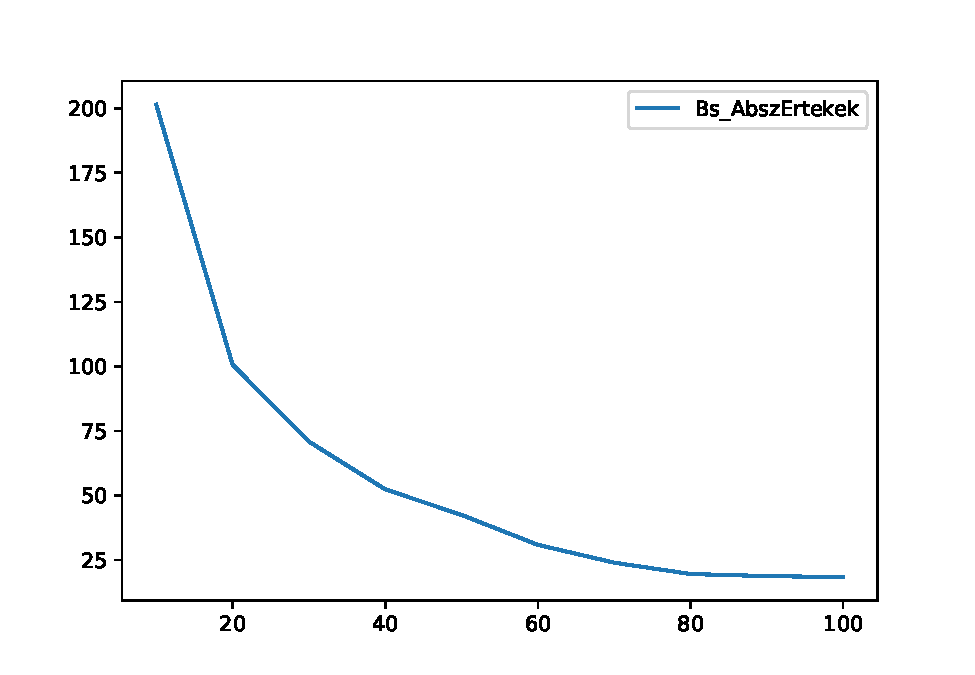
\includegraphics{_main_files/figure-latex/unnamed-chunk-239-1.pdf}

Szépen, gyakorlatilag exponenciális ütemben csökken a \(Bs\) abszolút érték, bár a \textbf{csökkenés nagysága \(n=90\)-ről \(n=100\)-ra már nem túl jelentős}! Ez azt jelenti, hogy \textbf{varianciák esetén a torzítás mértéke függ az \(n\) elemszámtól!} Minél nagyobb az elemszám, annál kisebb a torzítás mértéke, tehát az \(|Bs|\).

\section{A korrigált mintavariancia}\label{a-korriguxe1lt-mintavariancia}

A 2.1. fejezetben tapasztalt tényt, miszerint a mintavariancia \((s^*)^2\) a valós, sokasági \(\sigma^2\)-nek \textbf{aszimptotikusan torzítatlan becslése} fel lehet használni a \textbf{variancia torzítási probléma megoldására}.

Ugyebár azt tudjuk az szimptotikusan torzítatlanságból, hogy minél nagyobb az elemszám, annál kisebb a torzítás mértéke. Sőt, azt is meg lehet mondani, hogy \textbf{a mintavarianciák várható értéke, \(E\left((s^*)^2\right)\) arányaiban \(\frac{n-1}{n}\)-nel tér el a sokasági varianciától, \(\sigma^2\)-től}. Azaz igaz a következő egyenlőség: \[\frac{E\left((s^*)^2\right)}{\sigma^2}=\frac{n-1}{n}\]

Újrahasznosítva a \(Bs\)-ek meghatározására alkalmazott \texttt{for} ciklusos megoldásunkat, a \textbf{fenti összefüggés helyessége is ellenőrizhető \(n=\{10,20,30,...,90,100\}\) elemszámok mesetén}.

\begin{Shaded}
\begin{Highlighting}[]
\CommentTok{\# Üres lista létrehozása a (várható érték) / (sokasági variancia) hányadosok tárolására}
\NormalTok{Hanyados\_Lista }\OperatorTok{=}\NormalTok{ []}
\CommentTok{\# Üres lista létrehozása az (n{-}1)/n hányadosok tárolására}
\NormalTok{ElemszamHanyados\_Lista }\OperatorTok{=}\NormalTok{ []}
\CommentTok{\# Vizsgált elemszámok listájának létrehozása}
\CommentTok{\# 10 és 100 közötti egész számok felsoroltatása a \textquotesingle{}range\textquotesingle{} függvényben 10{-}es lépésközzel}
\CommentTok{\# Felső határ 101 a nyílt intervallum miatt}
\NormalTok{Elemszam\_Lista }\OperatorTok{=} \BuiltInTok{range}\NormalTok{(}\DecValTok{10}\NormalTok{, }\DecValTok{101}\NormalTok{, }\DecValTok{10}\NormalTok{)}

\CommentTok{\# Ciklus indítása}
\ControlFlowTok{for}\NormalTok{ AktualisElemszam }\KeywordTok{in}\NormalTok{ Elemszam\_Lista:}
\NormalTok{  AktualisMintaVetelek }\OperatorTok{=}\NormalTok{ MintaVetelek100Elem.iloc[:, }\DecValTok{0}\NormalTok{:AktualisElemszam].copy()}
\NormalTok{  AktualisMintaVetelek[}\StringTok{\textquotesingle{}Varianciak\textquotesingle{}}\NormalTok{] }\OperatorTok{=}\NormalTok{ np.std(AktualisMintaVetelek, axis }\OperatorTok{=} \DecValTok{1}\NormalTok{)}\OperatorTok{**}\DecValTok{2}
\NormalTok{  AktualisVarianciakAtlaga }\OperatorTok{=}\NormalTok{ np.mean(AktualisMintaVetelek[}\StringTok{\textquotesingle{}Varianciak\textquotesingle{}}\NormalTok{])}
\NormalTok{  Hanyados\_Lista.append(}\BuiltInTok{round}\NormalTok{(AktualisVarianciakAtlaga}\OperatorTok{/}\NormalTok{SokasagiVariancia, }\DecValTok{3}\NormalTok{))}
\NormalTok{  ElemszamHanyados\_Lista.append(}\BuiltInTok{round}\NormalTok{((AktualisElemszam }\OperatorTok{{-}} \DecValTok{1}\NormalTok{)}\OperatorTok{/}\NormalTok{AktualisElemszam, }\DecValTok{3}\NormalTok{))}

\CommentTok{\# Eredmények összefűzése data frame{-}be }
\NormalTok{Hanyados\_df }\OperatorTok{=}\NormalTok{ pd.DataFrame(}
  \BuiltInTok{list}\NormalTok{(}\BuiltInTok{zip}\NormalTok{(ElemszamHanyados\_Lista, Hanyados\_Lista)),}
\NormalTok{  columns}\OperatorTok{=}\NormalTok{[}\StringTok{\textquotesingle{}(n{-}1)/n\textquotesingle{}}\NormalTok{, }\StringTok{\textquotesingle{}VarhatoErtek/SokasagiVar\textquotesingle{}}\NormalTok{])}
\NormalTok{Hanyados\_df}
\end{Highlighting}
\end{Shaded}

\begin{verbatim}
##    (n-1)/n  VarhatoErtek/SokasagiVar
## 0    0.900                     0.896
## 1    0.950                     0.948
## 2    0.967                     0.964
## 3    0.975                     0.973
## 4    0.980                     0.978
## 5    0.983                     0.984
## 6    0.986                     0.988
## 7    0.988                     0.990
## 8    0.989                     0.990
## 9    0.990                     0.991
\end{verbatim}

Szuper, \textbf{aránylag szépen kijön a kétféle hányadosok közötti egyezőség}! :) Persze itt is van némi \textbf{eltérés, mivel csak \(10000\) db mintát vizsgálunk és nem az összes lehetségeset}, de ez még így is látványos egyezés! Így már \textbf{érthető, hogy a \(Bs\) abszolút értéke miért nem csökkent már látványosan \(n=90\)-ről \(n=100\)-ra: az \(\frac{n-1}{n}\) hányados mindkét esetben már elég kicsit volt, így a torzítás mértéke is!}

Viszont, ha a \(\frac{E\left((s^*)^2\right)}{\sigma^2}=\frac{n-1}{n}\) egyenlőség igaz, akkor azt átrendezve a következő összefüggésre jutunk: \[\sigma^2=\frac{n}{n-1} \times E\left((s^*)^2\right)\]

Konstans szorzót egy átlagolás (\(E(...)\)) eredményén alkalmazni ugyan az, mintha minden kiátlagolandó elemet felszoroztam volna azzal a szorzóval. Tehát az \(\frac{n}{n-1}\) bevihető a várható érték függvényen belülre: \[\sigma^2= E\left(\frac{n}{n-1} \times (s^*)^2\right)\]

Mindezek alapján pedig azt mondjatjuk, hogy \textbf{az \(s^2=\frac{n}{n-1} \times (s^*)^2\) módon KORRIGÁLT MINTAVARIANCIA már TORZÍTATLANUL becsli a valós sokasági varianciát, azaz \(\sigma^2\)-t!} Hiszen \(\sigma^2= E\left(s^2\right)\).

Tyűha, ez nagyon szépen hangzik! :) \textbf{Próbáljuk ki! Számoljuk ki a \(10000\) db \(n=100\) elemű mintában a korrigált mintavarianciákat, és nézzük meg azok átlagát (várható értékét)!}

\begin{Shaded}
\begin{Highlighting}[]
\CommentTok{\# Elemszám megadása külön változóban}
\NormalTok{n }\OperatorTok{=} \DecValTok{100}

\CommentTok{\# Korrigált varianciák}
\NormalTok{MintaVetelek100Elem[}\StringTok{\textquotesingle{}KorrigaltVar\textquotesingle{}}\NormalTok{] }\OperatorTok{=}\NormalTok{ (n}\OperatorTok{/}\NormalTok{(n}\OperatorTok{{-}}\DecValTok{1}\NormalTok{)) }\OperatorTok{*}\NormalTok{ MintaVetelek100Elem[}\StringTok{\textquotesingle{}Varianciak\textquotesingle{}}\NormalTok{]}

\CommentTok{\# Torzítatlanság ellenőrzése}
\NormalTok{KorrVarAtlaga }\OperatorTok{=}\NormalTok{ np.mean(MintaVetelek100Elem[}\StringTok{\textquotesingle{}KorrigaltVar\textquotesingle{}}\NormalTok{])}

\NormalTok{[KorrVarAtlaga, SokasagiVariancia]}
\end{Highlighting}
\end{Shaded}

\begin{verbatim}
## [1944.8360833702807, 1943.781182155494]
\end{verbatim}

\begin{Shaded}
\begin{Highlighting}[]
\BuiltInTok{round}\NormalTok{(KorrVarAtlaga }\OperatorTok{{-}}\NormalTok{ SokasagiVariancia, }\DecValTok{1}\NormalTok{)}
\end{Highlighting}
\end{Shaded}

\begin{verbatim}
## 1.1
\end{verbatim}

Győzelem! :) Ha \textbf{nem is szűnt meg teljesen a dolog, de láthatóan nagyon alacsony, majdnem elhanyagolható lett a \(Bs\) mértéke}! Sőt, már nem lefele torzítunk azzal a minimális \(1.1\)-gyel, hanem felfelé, ami egy szóródás becslésnél még a ``\emph{jobbik eset}''. Lásd a korábbi pénzügyi kockázat becslése példát. :) Ha \textbf{lenne több mintánk, akkor a korrekció ki is nullázná a \(Bs\)-t}.

Ezek alapján akkor jó lenne, ha \textbf{lenne valami beépített függvényünk} az \texttt{std} helyett, ami \textbf{mintaadatok esetén alapból a KORRIGÁLT SZÓRÁS \(s = \sqrt{s^2}=\sqrt{\frac{n}{n-1} \times (s^*)^2}\) értékét számolja}!

Nos, \textbf{valójában az} \texttt{std} \textbf{tud korrigált szórást számolni egy extra paraméter segítségével}. Ahhoz, hogy \textbf{megértsük a paraméter működését egy picit végig kell gondolni a korrigált szórás képletének a működését}.

Alapból a mintaadatok \(s^*\) szórását az alánbbi képlettel számoljuk: \[s^*=\sqrt{\frac{\sum_{i=1}^n{(y_i-\bar{y})^2}}{n}}\]

Azaz, megnézzük, hogy minden \(y_i\) mintaelem mennyivel tér el a minta \(\bar{y}\) átlagától, majd ezen eltéréseket négyzetre emelve összeadjuk és az összeget leosztjuk a minta \(n\) elemszámával, végül gyököt vonunk az egész hányadosból.
Ennek az értéknek a négyzete a sima, \emph{nem korrigált} variancia: \[(s^*)^2=\frac{\sum_{i=1}^n{(y_i-\bar{y})^2}}{n}\]

Ha a fenrti variancia képletet beszorozzuk \(\frac{n}{n-1}\)-gyel akkor a következő egyszerűséítéseket tehetjük: \[s^2=\frac{n}{n-1} \times \frac{\sum_{i=1}^n{(y_i-\bar{y})^2}}{n} = \frac{\sum_{i=1}^n{(y_i-\bar{y})^2}}{n-1}\]

Tehát, a \textbf{minta korrigált szórását úgy számoljuk ki mint a nem korrigáltat, csak a NEVEZŐBEN \(n-1\)-gyel osztunk, nem pedig \(n\)-nel}: \[s=\sqrt{\frac{\sum_{i=1}^n{(y_i-\bar{y})^2}}{n-1}}\]

Ezt az \textbf{eltérést a nevezőben} a \texttt{ddof\ =\ 1} \textbf{paraméter beállítással jelezzuk} a \texttt{numpy} csomag \texttt{std} függvényében. Könnyen kitalálható, hogy alapértelmezésben \texttt{ddof\ =\ 0} beállítással fut az \texttt{std} függvény. :)

Lássuk is a dolgot akcióban!

\begin{Shaded}
\begin{Highlighting}[]
\CommentTok{\# Korrigált varianciák \textquotesingle{}std\textquotesingle{}{-}vel}
\NormalTok{MintaVetelek100Elem[}\StringTok{\textquotesingle{}KorrigaltVar\_std\textquotesingle{}}\NormalTok{] }\OperatorTok{=}\NormalTok{ np.std(MintaVetelek100Elem.iloc[:,}\DecValTok{0}\NormalTok{:}\DecValTok{100}\NormalTok{], axis}\OperatorTok{=}\DecValTok{1}\NormalTok{, ddof }\OperatorTok{=} \DecValTok{1}\NormalTok{)}\OperatorTok{**}\DecValTok{2}

\CommentTok{\# Torzítatlanság ellenőrzése}
\NormalTok{KorrVarAtlaga\_std }\OperatorTok{=}\NormalTok{ np.mean(MintaVetelek100Elem[}\StringTok{\textquotesingle{}KorrigaltVar\_std\textquotesingle{}}\NormalTok{])}

\NormalTok{[KorrVarAtlaga\_std, SokasagiVariancia]}
\end{Highlighting}
\end{Shaded}

\begin{verbatim}
## [1944.8360833702802, 1943.781182155494]
\end{verbatim}

\begin{Shaded}
\begin{Highlighting}[]
\BuiltInTok{round}\NormalTok{(KorrVarAtlaga\_std }\OperatorTok{{-}}\NormalTok{ SokasagiVariancia, }\DecValTok{1}\NormalTok{)}
\end{Highlighting}
\end{Shaded}

\begin{verbatim}
## 1.1
\end{verbatim}

Királyság! Tökéletesen ugyan ott vagyunk, mint az előbb a manuális számolással! :)

\textbf{Szépen szakszavakkal összefoglalva} tehát az a fő tanulságunk, hogy

\begin{enumerate}
\def\labelenumi{\arabic{enumi}.}
\tightlist
\item
  A \textbf{sima mintavariancia (\((s^*)^2\)) a sokasági variancia \(\sigma^2\) TORZÍTOTT becslőfüggvénye}
\item
  A \textbf{korrigált mintavariancia (\(s^2\))} viszont \textbf{a sokasági variancia \(\sigma^2\) TORZÍTATLAN becslőfüggvénye}
\end{enumerate}

\section{A medián torzítatlansága}\label{a-mediuxe1n-torzuxedtatlansuxe1ga}

\textbf{Stat. 1-en nagyon fontos mutatónk volt a medián}, mint a vizsgált ismérv felezőpontja, hiszen nem volt érzékeny a kilógó értékekre az adatsorban, mint az átlag. \textbf{Nézzük meg} itt a Balaton átúszás 100 elemű mintáinak példáján, hogy ez a statisztikai paraméter \textbf{torzítatlanul becsülhető-e!}

\begin{Shaded}
\begin{Highlighting}[]
\CommentTok{\# Sokasági medián átúszási idő}
\NormalTok{SokasagiMedian }\OperatorTok{=}\NormalTok{ np.median(Balcsi.PERC)}

\CommentTok{\# Mintabeli mediánok kiszámítása}
\NormalTok{MintaVetelek100Elem[}\StringTok{\textquotesingle{}Medianok\textquotesingle{}}\NormalTok{] }\OperatorTok{=}\NormalTok{ np.median(MintaVetelek100Elem.iloc[:,}\DecValTok{0}\NormalTok{:}\DecValTok{100}\NormalTok{], axis}\OperatorTok{=}\DecValTok{1}\NormalTok{)}

\CommentTok{\# Mintabeli mediánok átlaga}
\NormalTok{MedianokAtlaga }\OperatorTok{=}\NormalTok{ np.mean(MintaVetelek100Elem[}\StringTok{\textquotesingle{}Medianok\textquotesingle{}}\NormalTok{])}

\CommentTok{\# Torzítatlanság ellenőrzése}
\NormalTok{[MedianokAtlaga, SokasagiMedian]}
\end{Highlighting}
\end{Shaded}

\begin{verbatim}
## [162.3393025, 162.26666666666668]
\end{verbatim}

\begin{Shaded}
\begin{Highlighting}[]
\BuiltInTok{round}\NormalTok{(MedianokAtlaga }\OperatorTok{{-}}\NormalTok{ SokasagiMedian, }\DecValTok{1}\NormalTok{)}
\end{Highlighting}
\end{Shaded}

\begin{verbatim}
## 0.1
\end{verbatim}

Olybá tűnik, hogy a medián a mintabeli mediánokkal \textbf{torzítatlanul becsülhető} A \(Bs(me) = E(me) - Me\) eltérés olyan minimális, hogy simán elhihető, hogy megszűnik, ha az összes lehetséges \(n=100\) lemeű mintát vizsgálnánk és nem csak \(10000\)-et.

\section{\texorpdfstring{A Standard Hiba (\emph{SH}) fogalma}{A Standard Hiba (SH) fogalma}}\label{a-standard-hiba-sh-fogalma}

Szép és jó, hogy megállapítottuk, hogy a mintaátlag, mintaarány, korrigált mintavariancia és mintamedián \textbf{torzítatlan becslőfüggvény}ei a nekik megfelelő sokasági \(\theta\) paramézereknek, de \textbf{mire jó ez nekünk a gyakorlatban, amikor csak egyetlen egy darab mintavételünk van?}

Hiszen, mint a 3-4. fejeuetekben tapasztaltuk, a torzítatlanság csak annyit mond, hogy ha van \textbf{nagyon-nagyon sok mintavételünk}, akkor a vizsgált statisztikai mutatónk/paraméterünk mintából számított értékei (becslőfüggvények) \textbf{átlagosan eltalálják a mutató valós, sokasági értékét}. De sajnos ebbe a \textbf{definícióba nagyon sok minden belefér}, és igazából \textbf{önmagában a mintavételi hibáról (MVH) nem mond semmit}.
Ezt a problémát nagyon jól érzékelteti a következő \emph{favicc}.

\begin{quote}
``Egy mérnök, egy fizikus és egy statisztikus együtt mennek vaddisznóra vadászni. Alig tesznek meg néhány lépést az erdőben, máris észrevesznek 150 méterre egy hatalmas példányt.
A mérnök felemeli a puskáját, céloz és lő, de három méterrel mellétalál jobbra. A fizikus így okoskodik:''Egy kis szellő fúj balról, ha kicsit balra célzok, akkor eltalálom.''
Ő is célbaveszi a szarvast, lő és három méterrel balra elvéti. A statisztikus felugrik, és örvendezni kezd:
``Megvan! Megvan! Eltaláltuk!''

\hfill -- Méltán Ismeretlen Szerző
\end{quote}

Ugyebár kedvenc viccbéli statisztikus azért örvendez, mivel a három méterrel jobbra és balra hibázó két lövés átlagban pont telibe kapta szegény vaddisznónkat!
Na, hát erről szól a \textbf{torzítatlanság} is:

\begin{itemize}
\tightlist
\item
  Le akarunk vadászni \emph{lövésekkel}, azaz \emph{mintavételekkel} egy statisztikai paraméter sokasági értékét, \(\theta\)-t.
\item
  Az első lövés, az 1. mintavételből származó becslőfüggvényünk értéke \(\hat{\theta}_1\)
\item
  A második lövés, a 2. mintavételből származó becslőfüggvényünk értéke \(\hat{\theta}_2\)
\item
  Ezek átlagban, azaz várható értékben eltallálják a keresett valós értéket, \(\theta\)-t: \(E(\hat{\theta})=\theta\)
\item
  Íme: ez a \emph{torzítatlan becslés} definíciója :)
\end{itemize}

Az statisztikai ``\(\hat{\theta}\)''-os vadászat és a vaddisznó vadász közti \textbf{analógia az alábbi ábrán szemléltethető}. \textbf{FONTOS} :)

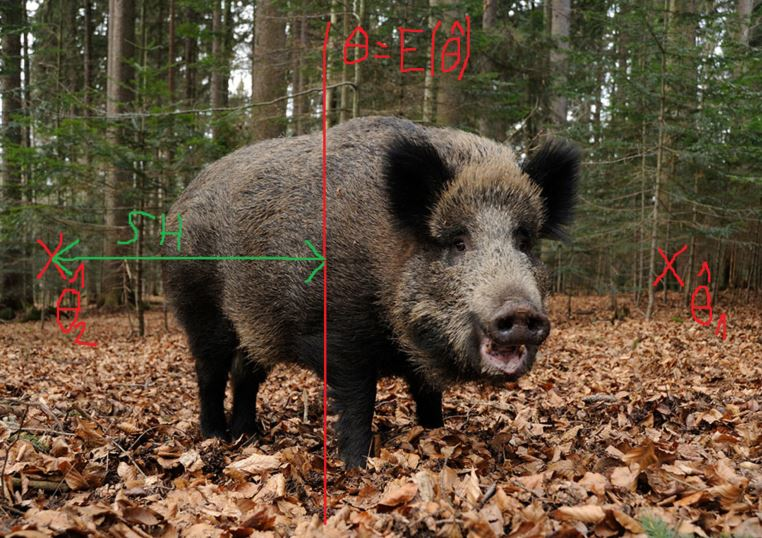
\includegraphics[width=0.5\textwidth,height=\textheight]{BiasBoar.jpg}

A fenti ábrán bejelöltem \textbf{zölddel} egy \textbf{tetszőleges \(\hat{\theta}_i\) és a valós, sokasági \(\theta\) közti távolság}ot. Valójában \textbf{ez az a távolság, amire kíváncsiak vagyunk egy tetszőleges FAE mintából számolt becslés és a keresett mutató sokasági értéke közötti távolság}! Hiszen a gyakorlatban \textbf{csak egy db mintavételünk van, és az egyetlen egy megfigyelt mintából kimókolt \(\hat{\theta}\) és \(\theta\) közti távolságot kéne kiszámolni}! Ez lenne ugyebár a \textbf{MVH}, amit kersünk!
Nos, a \textbf{torzítatlanságnak hála} van egy módszer, amivel ezt a \textbf{távolságot ki lehet számolni}! Hiszen, ha a torzítatlanság miatt \(E(\hat{\theta})=\theta\), akkor ez azt jelenti, hogy \textbf{a sok-sok mintából számolt \(\hat{\theta}_i\) értékek szórása épp a keresett zöld távolság}. Hiszen mi is a \textbf{szórás általános értelmezése}? Egy \textbf{véletlenszerűen kiválasztott elem az adatsorból várhatóan mennyivel tér el az átlagtól}. Hogyan fordul ez le a \(\hat{\theta}\)-ok adatsorára? Ha a \textbf{sok-sok lehetséges mintavételből kiválasztok egyet, akkor a kiválasztott mintából számolt \(\hat{\theta}\) várhatóan szórásnyival tér el} a \(\hat{\theta}\)-ok átlagától, azaz a \emph{torzítatlanság} miatt épp a \textbf{valós, sokasági \(\theta\) értékétől}.
Ebből az okfejtésből kiindulva \textbf{a\(\hat{\theta}\)-ok szórását standard mintavételi hibának, röviden csak standard hibának, ``SH''-nak nevezzük}.

Akkor ezen felbuzdulva \textbf{számoltassuk ki} pitonkával az \textbf{átlag és arány standard hibáit}, mint a \(\hat{\theta}\)-ként funkcionáló \textbf{mintaátlagok és minatarányok szórása}! Itt sima szórást kell stámolni, semmi korrekció nem kell az \texttt{std} függvényben.

\begin{Shaded}
\begin{Highlighting}[]
\NormalTok{SH\_Atlag }\OperatorTok{=}\NormalTok{ np.std(MintaVetelek100Elem.Atlagok)}
\NormalTok{SH\_Arany }\OperatorTok{=}\NormalTok{ np.std(MintaVetelek100Elem.Aranyok)}

\NormalTok{SH\_Atlag}
\end{Highlighting}
\end{Shaded}

\begin{verbatim}
## 4.402018186841923
\end{verbatim}

\begin{Shaded}
\begin{Highlighting}[]
\NormalTok{SH\_Arany}
\end{Highlighting}
\end{Shaded}

\begin{verbatim}
## 0.04667871960540553
\end{verbatim}

Mivel az \textbf{átlag és arány torzítatlan becslések}, így a \textbf{szórásként kiszámolt standard hibát a következőképpen lehet értelmezni}:

\begin{itemize}
\tightlist
\item
  100 elemű minták esetén \textbf{egy konkrét mintaátlag várhatóan \(4.4\) perccel tér el az átlagok átlagától, azaz a valós, sokasági átlagos átúszási időtől}.
\item
  \textbf{Egy konkrét 100 elemű mintában a Balatont 3 órán túl átúszók aránya várhatóan \(4.67\) százalékponttal tér el a teljes sokaság hasonló arányától}.
\end{itemize}

Hasonlóan működik a dolog ezen a szinten a varianciákra és mediánokra is. HF kiszámolni és értelmezni az eredményeket. :)

Viszont, \textbf{olybá tűnik, hogy nem vagyunk sokkal előrébb}. Mivel, bár a standard hiba megadja, hogy egy mintából számolt becslés várhatóan mennyivel tér el a valóságtól, de a \textbf{standard hiba (SH) kiszámolásához sok-sok mintavételre van szükség, hiszen ezekből a mintákból számolt \(\hat{\theta}\)-k szórásaként tudjuk az SH értéket megahtározni}!
Az kéne, hogy \textbf{az SH-t egyetlen egy mintavételből is valahogy ki tudjuk számolni}!

Erre \textbf{az átlag és az arány esetében van megoldásunk}. Ugyanis e két mutató esetében a \textbf{SH kifejezhető zárt formulával is}:

\begin{itemize}
\tightlist
\item
  \(SH(\bar{y})=\frac{\sigma}{\sqrt{n}}\)
\item
  \(SH(p)=\sqrt{\frac{P(1-P)}{n}}\)
\end{itemize}

Tehát, a \textbf{két standard hiba a sokasági szórás (\(\sigma\)) és a keresett sokasági arány (\(P\)) és a mintaelemszám \(n\) ismeretében megahtározahtó}. Próbáljuk is ki a dolgot.

\begin{Shaded}
\begin{Highlighting}[]
\NormalTok{n }\OperatorTok{=} \DecValTok{100}

\NormalTok{SH\_Atlag\_Formula }\OperatorTok{=}\NormalTok{ SokasagiSzoras }\OperatorTok{/}\NormalTok{ np.sqrt(n)}
\NormalTok{SH\_Arany\_Formula }\OperatorTok{=}\NormalTok{ np.sqrt((SokasagiArany }\OperatorTok{*}\NormalTok{ (}\DecValTok{1}\OperatorTok{{-}}\NormalTok{SokasagiArany))}\OperatorTok{/}\NormalTok{n)}

\NormalTok{[SH\_Atlag, SH\_Atlag\_Formula]}
\end{Highlighting}
\end{Shaded}

\begin{verbatim}
## [4.402018186841923, 4.408833385551663]
\end{verbatim}

\begin{Shaded}
\begin{Highlighting}[]
\NormalTok{[SH\_Arany, SH\_Arany\_Formula]}
\end{Highlighting}
\end{Shaded}

\begin{verbatim}
## [0.04667871960540553, 0.04700333404646558]
\end{verbatim}

Olybá tűnik, hogy \textbf{nagyjából egyezik a két érték}. :) A minimális eltérés megint abbók fakad, hogy nem az összes lehetséges mintát vizsgáltuk, csak \(10000\) db-ot, amikor a \(SH\)-kat a \(\hat{\theta}\)-ok szórásaként számoltuk ki.

Viszont, itt \textbf{megint az a probléma, hogy a \(SH\) kiszámításhoz olyan dolgokat kell ismerni, amiket egyetlen egy mintavétel esetén nem ismerünk}: sokasági szórás (\(\sigma\)) és a sokasági arány (\(P\)).
\textbf{NODE!} Ezeket az ismeretlenek legalább tudjuk \textbf{helyettesíteni az egy mintavételből számolt torzítatlan becslésükkel}: a \(P\)-t helyettesítjük \(p\)-vel, a \(\sigma\)-t pedig a korrigált szórással, \(s\)-el (hiszen egy torzítatlan becslése kell).

Ennyi ismerettel pedig akkor pl. az \(5.\) mintánk alapján a \(SH(\bar{y}) \approx \frac{s}{\sqrt{n}}\) és \(SH(p) \approx \sqrt{\frac{p(1-p)}{n}}\) \textbf{közelítő képletekkel} meg tudjuk már határozni a \(SH\)-kat.

\begin{Shaded}
\begin{Highlighting}[]
\NormalTok{n }\OperatorTok{=} \DecValTok{100}

\NormalTok{SH\_Atlag\_ÖtödikMinta }\OperatorTok{=}\NormalTok{ np.sqrt(MintaVetelek100Elem.Varianciak[}\DecValTok{4}\NormalTok{] }\OperatorTok{/}\NormalTok{ n)}
\NormalTok{SH\_Arany\_ÖtödikMinta }\OperatorTok{=}\NormalTok{ np.sqrt((MintaVetelek100Elem.Aranyok[}\DecValTok{4}\NormalTok{] }\OperatorTok{*}\NormalTok{ (}\DecValTok{1}\OperatorTok{{-}}\NormalTok{MintaVetelek100Elem.Aranyok[}\DecValTok{4}\NormalTok{]))}\OperatorTok{/}\NormalTok{n)}

\NormalTok{SH\_Atlag\_ÖtödikMinta}
\end{Highlighting}
\end{Shaded}

\begin{verbatim}
## 4.558455568470775
\end{verbatim}

\begin{Shaded}
\begin{Highlighting}[]
\NormalTok{SH\_Arany\_ÖtödikMinta}
\end{Highlighting}
\end{Shaded}

\begin{verbatim}
## 0.04702127178203499
\end{verbatim}

Nem tűpontos a \(SH\) közelítése, de azért \textbf{nagyságrendileg látszik, hogy jó nyomon járunk már egy mintavétel alapján is!} :)

Sajnos \textbf{hasonló közelítő képleteink a varianciák més mediánok esetén NINCSENEK}. Ott majd más trükkökkel próbáljuk kiszámolni az \(SH\)-kat egy mintavétel alapján. De erről majd pár anyaggal később. :)

Most még egy \textbf{fontos elnevezés: a \(SH^2\)-et gyakran nevezi a szaknyelv a becslőfüggvény VARIANCIÁJÁNAK}. Én nem szeretem ezt az elnevezést, mert könnyű összekeverni a minta vagy éppen a sokasági adatok varianciájával, de sok helyen használják ezt az elnevezést, így fontos tudni! Tehát, ha valahol \textbf{olyat olvastok, hogy a mintaátlagok varianciája ennnyi vagy a mintaarányok varianciája amannyi, akkor ott a költő az adott mutatók \(SH^2\)-re gonfolt}. Jelölni pedig az elnevezés alapján logikus módon így szokás a dolgot: \(SH^2(\hat{\theta})=Var(\hat{\theta})\)

Ennek kapcsán talán fontos megemlékezni \textbf{összefoglalásként arról, hogy itt a becsléselméletben milyen különböző szórásokkal, illetve varianciákkal találkoztunk}:

\begin{itemize}
\tightlist
\item
  \textbf{Sokasági szórás}: A sokaság elemeinek várható eltérése a sokaság átlagától. Jele: \(\sigma\).

  \begin{itemize}
  \tightlist
  \item
    Négyzete: sokasági variancia, \(\sigma^2\)
  \end{itemize}
\item
  \textbf{Korrigálatlan mintaszórás}: Egy db minta elemeinek várható eltérése az egy db mintánk átlagától. Jele: \(\sigma^*\)

  \begin{itemize}
  \tightlist
  \item
    Négyzete: korrigálatlan mintavariancia, \((s^*)^2\)
  \end{itemize}
\item
  \textbf{Korrigált mintaszórás}: Ugyan az, mint a korigálatlan mintaszórás, csak \emph{torzítatlan} becslést ad a valós, sokasági szóródásra. Jele: \(s\)

  \begin{itemize}
  \tightlist
  \item
    Négyzete: korrigált mintavariancia, \(s^2\)
  \end{itemize}
\item
  \textbf{Standard hiba}: Sok-sok mintából számolt becslőfüggvény, azaz \(\hat{\theta}\) szórása. \emph{Torzítatlanság esetén} egy konkrét mintából számolt becslőfüggvény eltérése a vizsgált \(\theta\) paraméter valós, sokasági értékétől. Jele: \(SH(\hat{\theta})\)

  \begin{itemize}
  \tightlist
  \item
    Négyzete: becslőfüggvény varianciája, \(Var(\hat{\theta})\)
  \end{itemize}
\end{itemize}

\subsection{A konzisztens becslés fogalma}\label{a-konzisztens-becsluxe9s-fogalma}

A standard hibáik formulájából az is kikövetkeztethető a \textbf{mintaátlag és mintaarány} becslőfüggvények esetében, hogy ezek \textbf{konzisztens becslések is a valós sokasági átlagra, arányra}.

Ugyanis, általánosságban \textbf{egy \(\hat{\theta}\) becslőfüggvény akkor konzisztens, ha \(SH\)-ja, a mintaelemszám (\(n\)) növelésével \(0\)-ba tart}:\[\lim_{n \rightarrow \infty}{SH(\hat{\theta})} = 0\]

Azaz, a egyre nagyobb a mintaméret, akkor a vizsgált statisztikai mutatónk egy mintából számított értéke (\(\hat{\theta}\)) egyre közelebb lesz a mutató valós, sokasági értékéhez (\(\theta\)).

Könnyen látható, hogy \textbf{mintaelemszám (\(n\)) függvényében, mind a mintaátlagok, mind a mintaarányok standard hibái \(f(n) \sim \frac{1}{n}\) stílusú hiperbola függvények, amik a végtelenbe tartó \(n\) nevező esetén \(0\)-ba tartanak}:\[\lim_{n \rightarrow \infty}{SH(\bar{y})} = \lim_{n \rightarrow \infty}{\frac{\sigma}{\sqrt{n}}} = 0\]

és \[lim_{n \rightarrow \infty}{SH(p)} = \lim_{n \rightarrow \infty}{\sqrt{\frac{P(1-P)}{n}}} = 0\]

\textbf{Rajzoljuk is ki a standard hiba függvényt mondjuk \(SH(\bar{y})\) esetében} \(n=\{10,20,...,200\}\) elemszámok mellett, és \textbf{látni fogjuk a hiperbola alakot}. Bár a dolog nem teljesen tiszta, mert a \(0\)-ba tartás sebesség a képlet alapján ``\emph{gyökös}''. :) Az ábrázolást végző Python kód logikája teljesen egyezik azzal, amit a \emph{2.1. fejezetben} is használtunk.

\begin{Shaded}
\begin{Highlighting}[]
\CommentTok{\# Üres lista létrehozása a különböző elemszámok mellett vett SH{-}k tárolására}
\NormalTok{SH\_Lista }\OperatorTok{=}\NormalTok{ []}
\CommentTok{\# Vizsgált elemszámok listájának létrehozása}
\CommentTok{\# 10 és 200 közötti egész számok felsoroltatása a \textquotesingle{}range\textquotesingle{} függvényben 10{-}es lépésközzel}
\CommentTok{\# Felső határ 201 a nyílt intervallum miatt}
\NormalTok{Elemszam\_Lista }\OperatorTok{=} \BuiltInTok{range}\NormalTok{(}\DecValTok{10}\NormalTok{, }\DecValTok{201}\NormalTok{, }\DecValTok{10}\NormalTok{)}

\CommentTok{\# Ciklus indítása SH{-}k számításához}
\ControlFlowTok{for}\NormalTok{ AktualisElemszam }\KeywordTok{in}\NormalTok{ Elemszam\_Lista:}
\NormalTok{  SH\_Lista.append(}\BuiltInTok{round}\NormalTok{(SokasagiSzoras }\OperatorTok{/}\NormalTok{ np.sqrt(AktualisElemszam), }\DecValTok{3}\NormalTok{))}

\CommentTok{\# Vizsgált elemszámok és a mért SH{-}k data frame{-}be rendezése}
\CommentTok{\# Ahol az elemszámok a sorindexek}
\NormalTok{SHData }\OperatorTok{=}\NormalTok{ pd.DataFrame(SH\_Lista, columns}\OperatorTok{=}\NormalTok{[}\StringTok{\textquotesingle{}SH\_Átlag\textquotesingle{}}\NormalTok{], index }\OperatorTok{=} \BuiltInTok{range}\NormalTok{(}\DecValTok{10}\NormalTok{, }\DecValTok{201}\NormalTok{, }\DecValTok{10}\NormalTok{))}

\CommentTok{\# Ábrázolás a \textquotesingle{}plot\textquotesingle{} metódussal: nem kell paraméterezni, mert csak egy oszlopunk van}
\NormalTok{SHData.plot()}
\NormalTok{plt.show()}
\end{Highlighting}
\end{Shaded}

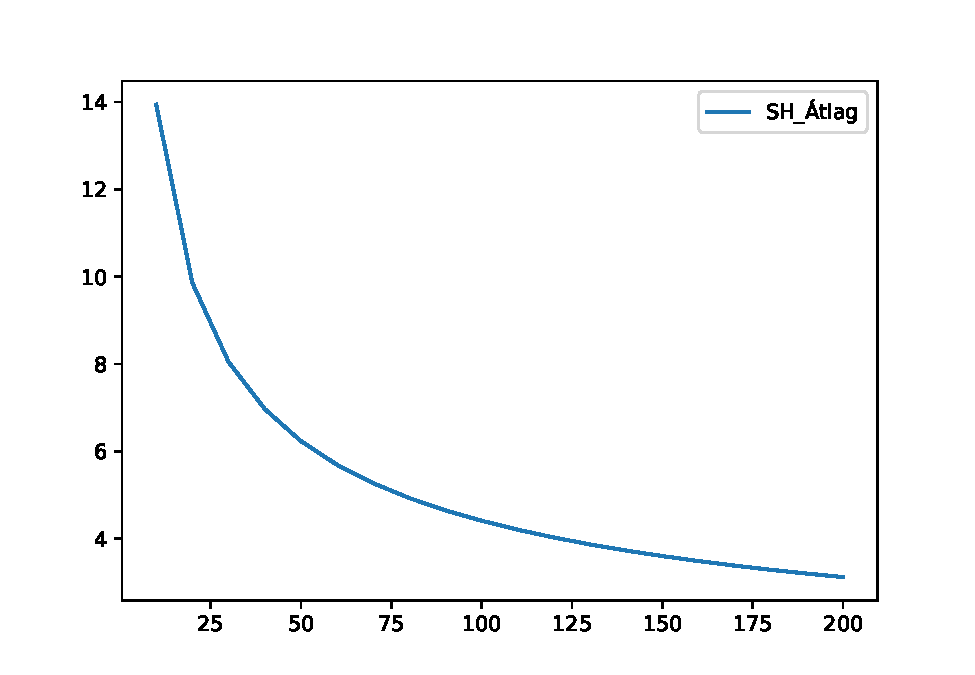
\includegraphics{_main_files/figure-latex/unnamed-chunk-247-3.pdf}

\section{\texorpdfstring{Az átlagos négyzetes hiba (\emph{MSE}) fogalma}{Az átlagos négyzetes hiba (MSE) fogalma}}\label{az-uxe1tlagos-nuxe9gyzetes-hiba-mse-fogalma}

Ugyebár arra jutottunk, hogy egy statisztikai paraméter becslőfüggvénynek a szórása, mint \textbf{standard hiba, csak akkor adja meg egy konkrét mintából számolt \(\hat{\theta}\) várható eltérését a valós, sokasági \(\theta\) értéktől, ha a becslőfüggvény torzítatlan}, mert ekkor egyezik meg \(\theta\) a sok-sok mintából számolt \(\hat{\theta}\)-ok átlagával, \(E(\hat{\theta})\)-val.

Ha nem torzítatlan becslőfüggvényről beszélünk, akkor \textbf{manuálisan ki tudjuk számolni a sok-sok mintából megadott \(\hat{\theta}\)-ok várható eltérését a valós, sokasági \(\theta\)-tól}. \textbf{Ez a mutató lesz a \(\hat{\theta}\) átlagos négyzetes hibája, angolul Mean Squared Error = MSE}. A számoláshoz simán a klasszikus variancia képletet kell alkalmazni a kövtekező módon: \[MSE(\hat{\theta})=\frac{\sum_{i=1}^K{(\hat{\theta}_i-\theta)^2}}{K}\]

A képletben \(K\) a mintavételek száma (nekünk most \(10000\)) \(\hat{\theta}_i\) egyszerűen az \(i\)-edik mintából számolt \(\hat{\theta}\) értéke.

\textbf{Számoljuk is ki az \(MSE\)-t, az egyetlen torzított becslőfüggvényre, a korrigálatlan mintavarianciára!} A képletnél muszáj Pythonban a \texttt{sum} függvényt alkalmazni, és ``\emph{manuálisan}'' lekódolni a formulát, mivel a beépített \texttt{std} függvénnyel \(\theta\) helyett \(E(\hat{\theta})\)-hoz viszonyítanánk, és a torzítottság miatt e két érték nem esik most egybe!

\begin{Shaded}
\begin{Highlighting}[]
\NormalTok{MSE\_Varianciak }\OperatorTok{=}\NormalTok{ np.}\BuiltInTok{sum}\NormalTok{((MintaVetelek100Elem.Varianciak }\OperatorTok{{-}}\NormalTok{ SokasagiVariancia)}\OperatorTok{**}\DecValTok{2}\NormalTok{)}\OperatorTok{/}\DecValTok{10000}

\NormalTok{MSE\_Varianciak}
\end{Highlighting}
\end{Shaded}

\begin{verbatim}
## 163460.24046057483
\end{verbatim}

Királyság! Namármost. Ez \textbf{a \(MSE\) érték} valójában a \textbf{becslés kétféje hibájának négyzetes összege}. Konkrétan \[MSE=SH^2+Bs^2\]

Ugyebár itt \textbf{egy \(\hat{\theta}\) becslőfüggvény eltérését a valós \(\theta\)-tól két lépcsőben lehet megközelíteni}:

\begin{enumerate}
\def\labelenumi{\arabic{enumi}.}
\tightlist
\item
  \(SH\): Mennyivel tér el egy konkrét minta \(\hat{\theta}\)-ja a becslések átlagától, \(E(\hat{\theta})\)-től.
\item
  \(Bs\): Mennyivel tér el a becslések átlaga a valós \(\theta\)-tól: \(Bs = E(\hat{\theta}) - \theta\)
\end{enumerate}

És ha kiszámoljuk a gyakorlatban, akkor látjuk, hogy az E\(MSE\) tényleg \textbf{ennek a fenti kétféle hibának az összege}.

\begin{Shaded}
\begin{Highlighting}[]
\NormalTok{Bs\_Varianciak }\OperatorTok{=}\NormalTok{ np.mean(MintaVetelek100Elem.Varianciak) }\OperatorTok{{-}}\NormalTok{ SokasagiVariancia}
\NormalTok{SH\_Varianciak }\OperatorTok{=}\NormalTok{ np.std(MintaVetelek100Elem.Varianciak)}

\NormalTok{MSE\_Varianciak\_Összeggel }\OperatorTok{=}\NormalTok{ Bs\_Varianciak}\OperatorTok{**}\DecValTok{2} \OperatorTok{+}\NormalTok{ SH\_Varianciak}\OperatorTok{**}\DecValTok{2}

\NormalTok{[MSE\_Varianciak, MSE\_Varianciak\_Összeggel]}
\end{Highlighting}
\end{Shaded}

\begin{verbatim}
## [163460.24046057483, 163460.2404605743]
\end{verbatim}

Jé, tényleg jó az összeges logikánk is! :)

Természetesen, ahol \textbf{torzítatlan a becslés, ott a \(Bs=0\) miatt az \(MSE = SH^2\) azonosság áll}. Vegyük \textbf{pl. a mintaarányok esetét}.

\begin{Shaded}
\begin{Highlighting}[]
\NormalTok{MSE\_Aranyok }\OperatorTok{=}\NormalTok{ np.}\BuiltInTok{sum}\NormalTok{((MintaVetelek100Elem.Aranyok }\OperatorTok{{-}}\NormalTok{ SokasagiArany)}\OperatorTok{**}\DecValTok{2}\NormalTok{)}\OperatorTok{/}\DecValTok{10000}
\NormalTok{SH\_Aranyok }\OperatorTok{=}\NormalTok{ np.std(MintaVetelek100Elem.Aranyok)}

\NormalTok{[MSE\_Aranyok, SH\_Aranyok}\OperatorTok{**}\DecValTok{2}\NormalTok{]}
\end{Highlighting}
\end{Shaded}

\begin{verbatim}
## [0.0021789054991602453, 0.0021789028640000706]
\end{verbatim}

ExcellenT! :)

\subsection{Különböző becslőfüggvények összehasonlítása}\label{kuxfcluxf6nbuxf6zux151-becslux151fuxfcggvuxe9nyek-uxf6sszehasonluxedtuxe1sa}

Az \(MSE\)-t kiválóan lehet hasznosítani, mint egy olyan \textbf{mérőszámot, amivel választani tudunk egy \(\theta\) sokasági paraméterre adott több lehetséges \(\hat{\theta}\) becslőfüggvény alternatíva közül}. Kiváló \textbf{példa erre az \((s^*)^2\) és \(s^2\), mint két alternatív becslőfüggény a sokasági variancia, \(\sigma^2\) becslésére}.

Mondhatnánk erre a kérdésre válaszként csípőből azt, hogy \textbf{``de hát a torzítatlan becslőfüggvény biztos jobb''}. Nos nem feltétlenül. Mert mi van \textbf{ha egy torzított becslés standard hibája annyival kisebb a torzítatlannál, hogy az ellensúlyozza a torzítás mértékét}, és a végén egy ``lövés'' (azaz \(\hat{\theta}\) becslés) a torzított becslőfüggvényből közelebb esik a valós \(\theta\)-hoz, mint a torzítatlan becslésből származó ``lövés''.

Ezt nagyon jól lehet érzékeltetni az 5. fejezet vaddisznó vadászatos példáján egy másik nézőpontból: \textbf{mi van ha a torzítatlan becslésnek akkor a standard hibája, hogy egy konkrét ``lövés'' (azaz \(\hat{\theta}\) becslés) jóval messzebb lesz a valós \(\theta\)-tól, mint egy torzított becslőfüggvényből származó becslés?}

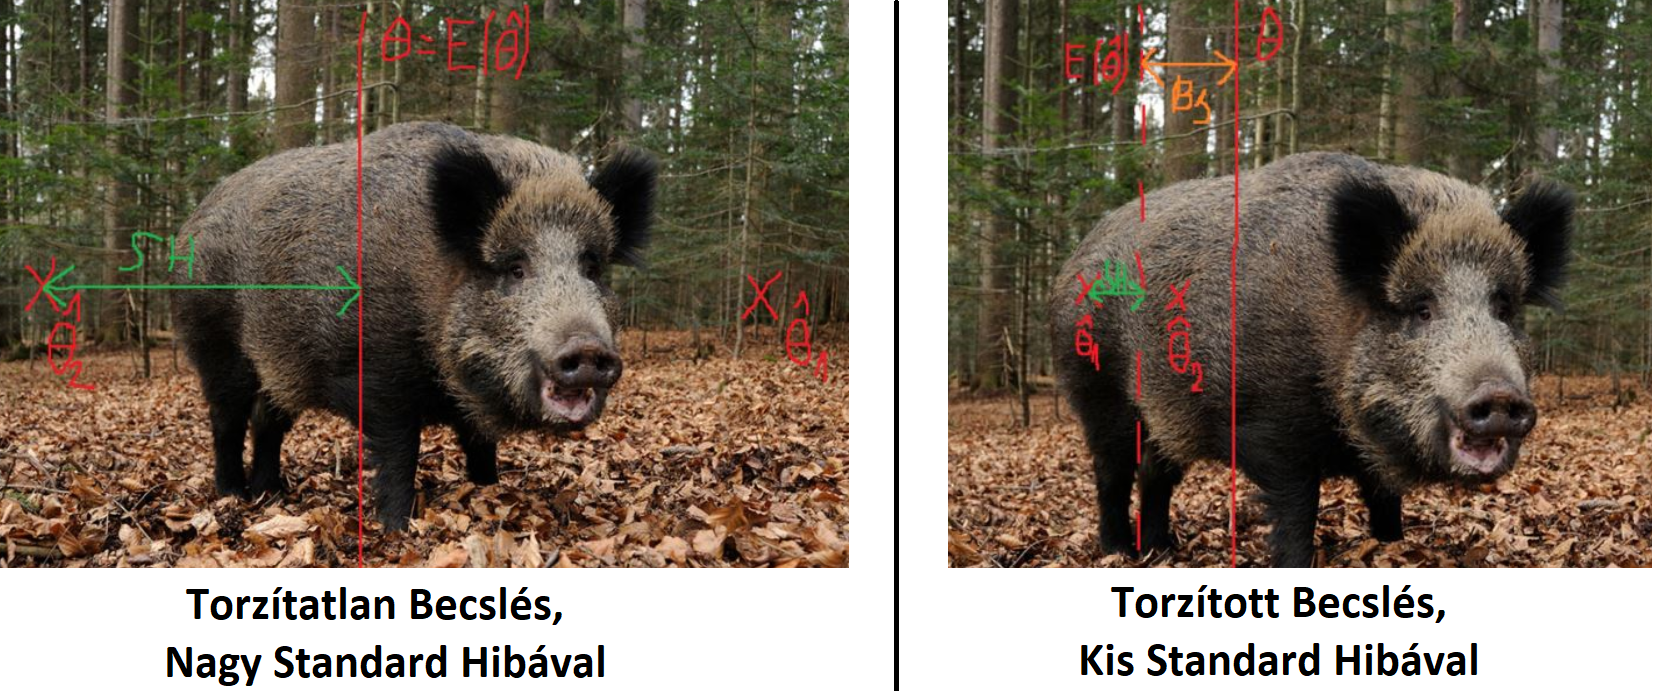
\includegraphics[width=0.9\textwidth,height=\textheight]{BiasBoarCompare.png}

Az ábrán látható, hogy \textbf{egy enyhén ``balra'' torzított becslőfüggvényből származó, de kis standard hibájú \(\hat{\theta}_i\) becslések még eltalálják a vaddisznót, de a torzítatlan becslések, bár sok-sok mintavétel átlagában nagyon jól működnek, de egy konkrét \(\hat{\theta}_i\) lövésnek akkora a standard hibája, hogy nagyon messzire elvéti azt a vaddisznót!}

Tehát a fenti jelenség miatt, ha \textbf{egy adott \(\theta\)-ra több becslőfüggvény közül kell választanunk, akkor azt az \(MSE\) alapján} szabad csak megtennünk, mert az egyszerre veszi figyelembe a torzítás mértékét és a standard hibát is.

Lássuk a dolgot a gyakorlatban: \textbf{Mi a jobb becslés a sokasági varianciára? A korrigált vagy a korrigálatlan mintavariancia?}

\begin{Shaded}
\begin{Highlighting}[]
\CommentTok{\# Torzított becslés = Korrigálatlan mintavar.}
\NormalTok{Bs\_Varianciak }\OperatorTok{=}\NormalTok{ np.mean(MintaVetelek100Elem.Varianciak) }\OperatorTok{{-}}\NormalTok{ SokasagiVariancia}
\NormalTok{SH\_Varianciak }\OperatorTok{=}\NormalTok{ np.std(MintaVetelek100Elem.Varianciak)}

\NormalTok{MSE\_Varianciak }\OperatorTok{=}\NormalTok{ Bs\_Varianciak}\OperatorTok{**}\DecValTok{2} \OperatorTok{+}\NormalTok{ SH\_Varianciak}\OperatorTok{**}\DecValTok{2}

\CommentTok{\# Torzítatlan becslés = Korrigált mintavar.}
\NormalTok{SH\_KorrVarianciak }\OperatorTok{=}\NormalTok{ np.std(MintaVetelek100Elem.KorrigaltVar)}

\NormalTok{MSE\_KorrVarianciak }\OperatorTok{=} \DecValTok{0} \OperatorTok{+}\NormalTok{ SH\_KorrVarianciak}\OperatorTok{**}\DecValTok{2}

\NormalTok{[MSE\_Varianciak, MSE\_KorrVarianciak]}
\end{Highlighting}
\end{Shaded}

\begin{verbatim}
## [163460.2404605743, 166433.95684503784]
\end{verbatim}

Hoppá, olybá tűnik, hogy \(MSE((s^*)^2) < MSE(s^2)\), tehát a \textbf{nem korrigált mintavariancia van közelebb a valós, sokasági \(\sigma^2\)-hez egy ``átlagos'' mintavétel esetén, hanem a sima korrigálatlan verzió}.
Ugyanakkor az \textbf{adatsor bizonytalanságának, szóródásának ``rendszeres'' alábecslése a legtöbb esetben nagyobb probléma, mint a némileg magasabb standard hiba}. Tehát, \textbf{bár összességében, azaz \(MSE\)-ben az \((s^*)^2\) mintavételi hibája kisebb, mint \(s^2\)-nek, de a kisebb hiba iránya ``lefelé'' van a torzítás miatt}, és ezt nem szeretjük itt most. Inkább \textbf{bevállalunk egy valamivel nagyobb, de ``szimmetrikus'' hibát}.
Így \textbf{variancia esetében} felülírjuk az \(MSE\) döntését, és a \textbf{korrigált mintavarianciát használjuk a legtöbb esetben}. Vagy másképpen fogalmazva azt mondhatjuk, hogy variancia esetén nagyobb súlyt helyezünk \(MSE\)-ben a \(Bs^2\)-re, mint a \(SH^2\)-re, és nem egyenlő mértékben preferáljuk a csökkenésüket.
Pl. az \textbf{átlag standard hibájának \(\frac{s}{\sqrt{n}}\) elvű közekítésénél ez azért is jogos, mert a korrigálatlan mintaszórás használata esetén egy mintaátlag távolságát a valós, sokasági átlagtól az ``átlagos mintavételben'' alábecsülnénk, ami azért kellemetlen}. :)

Ha \textbf{két torzítatlan becslőfüggvény közül kell választanunk, akkor simán választhatjuk azt, aminek a standard hibája kisebb, hiszen ilyenkor ez egyben azt is jelenti, hogy az \(MSE\)-je is kisebb}, mivel \(Bs^2=0\). Ezt hívják úgy is a szakirodalomban, mint a \textbf{hatásosság kritériuma: Két becslőfüggvény közül az a hatásosabb, amelynek \(SH\)-ja kisebb}. :)

\chapter{A sokasági átlag intervallumbecslése}\label{a-sokasuxe1gi-uxe1tlag-intervallumbecsluxe9se}

\section{Ismétlés: Az átlag standard hibája a Balaton átúszás eredményeken}\label{ismuxe9tluxe9s-az-uxe1tlag-standard-hibuxe1ja-a-balaton-uxe1tuxfaszuxe1s-eredmuxe9nyeken}

Ugyebár a 3. heti tananyagban a 2022-es Balaton átúszás résztvevőinek időeredményeit vizsgáltuk mintavételi és becsléselméleti szempontból elég alaposan. Töltsük is be egy \texttt{pandas} data frame-be ismét a LIDLBalaton2022.xlsx fájl adatait. Ebben az Excelben megvan az összes résztvevő időeredménye a \texttt{PERC} oszlopban. Ez az adatsor lesz most nekünk tehát a \textbf{sokaságunk}.

\begin{Shaded}
\begin{Highlighting}[]
\CommentTok{\# Elemzéshez és ábrázoláshoz szükséges csomagok betöltése}
\ImportTok{import}\NormalTok{ numpy }\ImportTok{as}\NormalTok{ np}
\ImportTok{import}\NormalTok{ pandas }\ImportTok{as}\NormalTok{ pd}
\ImportTok{import}\NormalTok{ matplotlib.pyplot }\ImportTok{as}\NormalTok{ plt}
\ImportTok{import}\NormalTok{ scipy.stats }\ImportTok{as}\NormalTok{ stats}

\CommentTok{\# Adatbeolvasás data frame{-}be}
\NormalTok{Balcsi }\OperatorTok{=}\NormalTok{ pd.read\_excel(}\StringTok{"LIDLBalaton2022.xlsx"}\NormalTok{)}

\NormalTok{Balcsi.info()}
\end{Highlighting}
\end{Shaded}

\begin{verbatim}
## <class 'pandas.core.frame.DataFrame'>
## RangeIndex: 9751 entries, 0 to 9750
## Data columns (total 3 columns):
##  #   Column  Non-Null Count  Dtype  
## ---  ------  --------------  -----  
##  0   Nev     9751 non-null   object 
##  1   Nem     9751 non-null   object 
##  2   PERC    9751 non-null   float64
## dtypes: float64(1), object(2)
## memory usage: 228.7+ KB
\end{verbatim}

\begin{Shaded}
\begin{Highlighting}[]
\NormalTok{Balcsi.head()}
\end{Highlighting}
\end{Shaded}

\begin{verbatim}
##                    Nev Nem        PERC
## 0           Aba Attila   F  142.416667
## 1        Abaffy Károly   F  197.883333
## 2        Abaffy Kornél   F  197.983333
## 3  Abelovszki Hajnalka   N  182.000000
## 4   Abért Valentin ifj   F  222.516667
\end{verbatim}

Meg is van akkor mind az \(N=9751\) részvevőnk. Ebben a tananyagban \textbf{most kizárólag az időeredmények átlagának becslésével} fogunk foglalkozni.
Úgyhogy \textbf{számoljuk is ki}, hogy az összes átúszó, azaz a \textbf{sokaság}, tekintetében mi az \textbf{időeredmények átlaga} (\(\mu=\bar{Y}\)). Ezen kívül majd jól jön még nekünk referenciaként az időeredméynek sokasági \textbf{szórása} (\(\sigma\)) is.

\begin{Shaded}
\begin{Highlighting}[]
\NormalTok{SokasagiAtlag }\OperatorTok{=}\NormalTok{ np.mean(Balcsi.PERC)}
\NormalTok{SokasagiSzoras }\OperatorTok{=}\NormalTok{ np.std(Balcsi.PERC)}

\NormalTok{SokasagiAtlag}
\end{Highlighting}
\end{Shaded}

\begin{verbatim}
## 167.52914060096398
\end{verbatim}

\begin{Shaded}
\begin{Highlighting}[]
\NormalTok{SokasagiSzoras}
\end{Highlighting}
\end{Shaded}

\begin{verbatim}
## 44.08833385551663
\end{verbatim}

Ezeka alapján tudjuk tehát, hogy egy átlagos Balaton átúszó \(\mu=165.5\) perc alatt teljesítette a távot, amitől egy konkrét versenyző saját időeredménye várhatóan \(\sigma=44.1\) perccel tér el.

\textbf{Az átlag becslése során} az a feladatunk, hogy \textbf{ezt a \(\mu=165.5\) perces átlagot valahogy ``megtippeljük''} egy visszatevéses véletlen (azaz FAE) \textbf{minta adatai alapján}.

Tehát, \textbf{vegyünk is egy \(n=100\) elemű mintát a Balatonátúszók sokaságából} a kedvenc \(1992\)-es véletlen magunk mellett, és nézzük meg, hogy \textbf{mennyi a mintaátlag, azaz \(\bar{y}\) értéke}.

\begin{Shaded}
\begin{Highlighting}[]
\NormalTok{BalcsiMinta }\OperatorTok{=}\NormalTok{ Balcsi.sample(n }\OperatorTok{=} \DecValTok{100}\NormalTok{, replace }\OperatorTok{=} \VariableTok{True}\NormalTok{, random\_state }\OperatorTok{=} \DecValTok{1992}\NormalTok{)}

\NormalTok{MintaAtlag }\OperatorTok{=}\NormalTok{ np.mean(BalcsiMinta.PERC)}

\NormalTok{MintaAtlag}
\end{Highlighting}
\end{Shaded}

\begin{verbatim}
## 164.44033333333334
\end{verbatim}

Tehát ebben az \(n=100\) elemű \textbf{mintában az átlagos átúszási idő \(164.4\) perc}. A 3. heti tananyagban elvégzett okoskodásunk alapján a \textbf{mintaátlag alapján úgy tudjuk lehatárolni a sokasági átlag (\(\mu\)) értékét, hogy a mintaátlag értékre rámérem \(\pm\) annak standard hibáját}. Hiszen a standard hiba megmutatja, hogy egy véletlenszerűen kiválasztott mintavétel átlaga várhatóan mennyivel tér el a valós sokasági átlagtól (mivel a \(\bar{y}\) mintaátlag alapból egy torzítatéan becslőfüggvénye a \(\mu\) sokasági átlagnak).
A gondolatmenet alapján tehát azt mondhatjuk, hogy a \textbf{sokasági átlag várhatóan mintaátlag \(\pm\) standard hiba által lehatárolt intervallumban nyugszik}.

Jó hír, hogy ugyebár az \textbf{átlag standard hibája sokasági szórás osztva gyök alatt mintaelemszám}, azaz \(\frac{\sigma}{\sqrt{n}}\) képlettel számolható, aminek az értékét egy mintavétel alapján is meg tudjuk közelíteni, ha a sokasági szórást, annak torzítatlan becslésével a \textbf{korrigált mintaszórás}sal helyettesítjük. Tehát, az \textbf{egy szem \(n=100\) mintából a standard hiba értéke az \(\frac{s}{\sqrt{n}}\) képlettel megközelíthető}.

Ez alapján akkor az alábbi számolást tudjuk elkövetni a mintánkon.

\begin{Shaded}
\begin{Highlighting}[]
\NormalTok{n }\OperatorTok{=} \DecValTok{100}
\NormalTok{s }\OperatorTok{=}\NormalTok{ np.std(BalcsiMinta.PERC, ddof }\OperatorTok{=} \DecValTok{1}\NormalTok{) }\CommentTok{\# figyeljünk a korrekcióra!}
\NormalTok{SH }\OperatorTok{=}\NormalTok{ s}\OperatorTok{/}\NormalTok{np.sqrt(n)}

\NormalTok{[MintaAtlag }\OperatorTok{{-}}\NormalTok{ SH, MintaAtlag }\OperatorTok{+}\NormalTok{ SH]}
\end{Highlighting}
\end{Shaded}

\begin{verbatim}
## [160.55804594814538, 168.3226207185213]
\end{verbatim}

Az eredményünk alapján a valós, sokasági átlag (\(\mu\)) várhatóan \(160.6\) és \(168.3\) perc között, azaz a \([160.6,168.3]\) intervallumban helyezkedik el. Nos, \textbf{az intervallumos becslésünk helyes is, hiszen a valós sokasági átlag uygebár \(\mu=167.5\) perc, ami tényleg benne van a mintánk alapján lehatárolt intervallumban}.

\section{A mintaátlagok eloszlása}\label{a-mintauxe1tlagok-eloszluxe1sa}

Na jó-jó, egy mintavétel esetén szerencsénk is lehetett. \textbf{Mennyire működik ez a standard hibás módszer jól sok-sok \(n=100\) mintavétel esetében?} Töltsük csak be egy data frame-be azt a táblát, ami \(10000\) db \(n=100\) FAE mintavétel adatait tartalmazza! Az átlalam generált Excel, ami tartalmazza a \(10000\) minta adatait innen érhető el.

\begin{Shaded}
\begin{Highlighting}[]
\NormalTok{MintaVetelek100Elem }\OperatorTok{=}\NormalTok{ pd.read\_excel(}\StringTok{"MintaDataFrame.xlsx"}\NormalTok{)}
\NormalTok{MintaVetelek100Elem}
\end{Highlighting}
\end{Shaded}

\begin{verbatim}
##            Elem1       Elem2       Elem3  ...      Elem98      Elem99     Elem100
## 0     164.800000  129.066667  156.166667  ...  207.350000  159.666667  165.883333
## 1     152.516667  212.483333  152.900000  ...  307.266667  119.783333  128.216667
## 2     145.666667  185.266667  169.516667  ...  167.733333  228.366667  215.633333
## 3     185.683333  120.333333  201.250000  ...  182.766667  177.666667  112.450000
## 4     117.483333  142.350000  320.266667  ...  188.566667  189.166667   99.916667
## ...          ...         ...         ...  ...         ...         ...         ...
## 9995  162.333333   83.350000  146.750000  ...  164.250000  131.933333  128.183333
## 9996  100.416667  161.433333  187.366667  ...  160.483333  168.416667  209.300000
## 9997  146.450000  160.783333  165.483333  ...  158.816667  167.733333  183.400000
## 9998  139.250000  140.466667  130.933333  ...  153.616667  112.366667  196.050000
## 9999  147.316667  173.450000  106.100000  ...  185.616667  171.800000  135.166667
## 
## [10000 rows x 100 columns]
\end{verbatim}

Oké, az eredményből látjuk is, hogy úgy néz ki a data frame, hogy \textbf{1 sor tartalmaz 1 db 100 elemű mintát és a mintaelemeket} (tehát a mintába besorsolt versenyző percben mért időeredményét) \textbf{az oszlopkban tároljuk}.

Akkor most \textbf{minden minta esetében számoljuk ki a \(\bar{y} \pm SH\) intervallumot}, és nézzük meg, hogy a valós \textbf{sokasági átlag} (\(\mu\)) \textbf{beleesik-e} az intervallumba! Annyi \textbf{előnyt is adjunk magunknak, hogy a standard hibát a sokasági szórás, azaz \(\sigma\) ismeretében számoljuk ki}. Tehát a \(SH = \frac{\sigma}{\sqrt{n}}\) képletet alkalmazzuk. Ugye ez annyiban előny, hogy \(\sigma\)-t egy db 100 elemű minta vizsgálata esetén NEM ismerjük!
A számolás során figyeljünk arra, hogy a \texttt{numpy} függvényeket \texttt{axis\ =\ 1} paraméterrel hazsnáljuk, hiszen egy db minta elemei a sorokban vannak. Illetve, a számolást mindig szorítsuk le a data frame első \(100\) oszlopára, hiszen a data frame oszlopait folyamatosan bővíteni fogjuk!

\begin{Shaded}
\begin{Highlighting}[]
\NormalTok{n }\OperatorTok{=} \DecValTok{100}
\NormalTok{SH }\OperatorTok{=}\NormalTok{ SokasagiSzoras }\OperatorTok{/}\NormalTok{ np.sqrt(n)}

\NormalTok{MintaVetelek100Elem[}\StringTok{\textquotesingle{}AtlagAlsoHatar\textquotesingle{}}\NormalTok{] }\OperatorTok{=}\NormalTok{ np.mean(MintaVetelek100Elem.iloc[:,}\DecValTok{0}\NormalTok{:}\DecValTok{100}\NormalTok{], axis }\OperatorTok{=} \DecValTok{1}\NormalTok{) }\OperatorTok{{-}}\NormalTok{ SH}
\NormalTok{MintaVetelek100Elem[}\StringTok{\textquotesingle{}AtlagFelsoHatar\textquotesingle{}}\NormalTok{] }\OperatorTok{=}\NormalTok{ np.mean(MintaVetelek100Elem.iloc[:,}\DecValTok{0}\NormalTok{:}\DecValTok{100}\NormalTok{], axis }\OperatorTok{=} \DecValTok{1}\NormalTok{) }\OperatorTok{+}\NormalTok{ SH}
\NormalTok{MintaVetelek100Elem}
\end{Highlighting}
\end{Shaded}

\begin{verbatim}
##            Elem1       Elem2  ...  AtlagAlsoHatar  AtlagFelsoHatar
## 0     164.800000  129.066667  ...      166.852833       175.670500
## 1     152.516667  212.483333  ...      153.617667       162.435333
## 2     145.666667  185.266667  ...      167.870000       176.687667
## 3     185.683333  120.333333  ...      159.025333       167.843000
## 4     117.483333  142.350000  ...      162.144000       170.961667
## ...          ...         ...  ...             ...              ...
## 9995  162.333333   83.350000  ...      159.273500       168.091167
## 9996  100.416667  161.433333  ...      159.924000       168.741667
## 9997  146.450000  160.783333  ...      159.293500       168.111167
## 9998  139.250000  140.466667  ...      162.015000       170.832667
## 9999  147.316667  173.450000  ...      168.641500       177.459167
## 
## [10000 rows x 102 columns]
\end{verbatim}

Oké, akkor \textbf{meg is vannak} az átlag intervallumos \textbf{becslés}ének \textbf{alsó-felső határai}. \textbf{Számoljuk} akkor \textbf{ki a találati arányt}!
A számoláshoz azt a trükköt alkalmazzuk, amit a 2. heti tananyagban sütüttünk el: a \texttt{AdatokEgyben{[}\textquotesingle{}Normal\textquotesingle{}{]}\ \textless{}\ 100} parancs egy \texttt{bool} tömböt ad vissza, amit összegezve megkapjuk a ``\emph{kedvező esetek}'', vagyis a \(\mu\)-t helyesen eltaláló intervallumok darabszámát.

\begin{Shaded}
\begin{Highlighting}[]
\NormalTok{MintaVetelekSzama }\OperatorTok{=} \BuiltInTok{len}\NormalTok{(MintaVetelek100Elem)}

\NormalTok{np.}\BuiltInTok{sum}\NormalTok{((MintaVetelek100Elem[}\StringTok{\textquotesingle{}AtlagAlsoHatar\textquotesingle{}}\NormalTok{] }\OperatorTok{\textless{}}\NormalTok{ SokasagiAtlag) }\OperatorTok{\&}\NormalTok{ (MintaVetelek100Elem[}\StringTok{\textquotesingle{}AtlagFelsoHatar\textquotesingle{}}\NormalTok{] }\OperatorTok{\textgreater{}}\NormalTok{ SokasagiAtlag)) }\OperatorTok{/}\NormalTok{ MintaVetelekSzama}
\end{Highlighting}
\end{Shaded}

\begin{verbatim}
## 0.684
\end{verbatim}

Nos, olybá tűnik, hogy a \(\bar{y} \pm SH\) módszer csak a \textbf{mintavételek kb. \(68\%\)-ban találja el a valós, sokasági átalgot, azaz \(\mu\)-t!} Gáz Géza! Azért ennél nagyobb találati arányt szeretnénk! Mondjuk legalább valami \(90\%\) környékét.

Ahhoz, hogy megértsük miért alakul gyéren ennek a módszernek találati aránya, \textbf{nézzünk csak rá az \(\bar{y}\) mintaátlagok hisztogramjára!} Most a hisztogramon nem optimalizálom az osztályközök számát, elfogadom a \texttt{numpy} alapbeállításait.

\begin{Shaded}
\begin{Highlighting}[]
\NormalTok{MintaVetelek100Elem[}\StringTok{\textquotesingle{}MintaAtlagok\textquotesingle{}}\NormalTok{] }\OperatorTok{=}\NormalTok{ np.mean(MintaVetelek100Elem.iloc[:,}\DecValTok{0}\NormalTok{:}\DecValTok{100}\NormalTok{], axis}\OperatorTok{=}\DecValTok{1}\NormalTok{)}

\NormalTok{MintaVetelek100Elem.MintaAtlagok.hist()}
\end{Highlighting}
\end{Shaded}

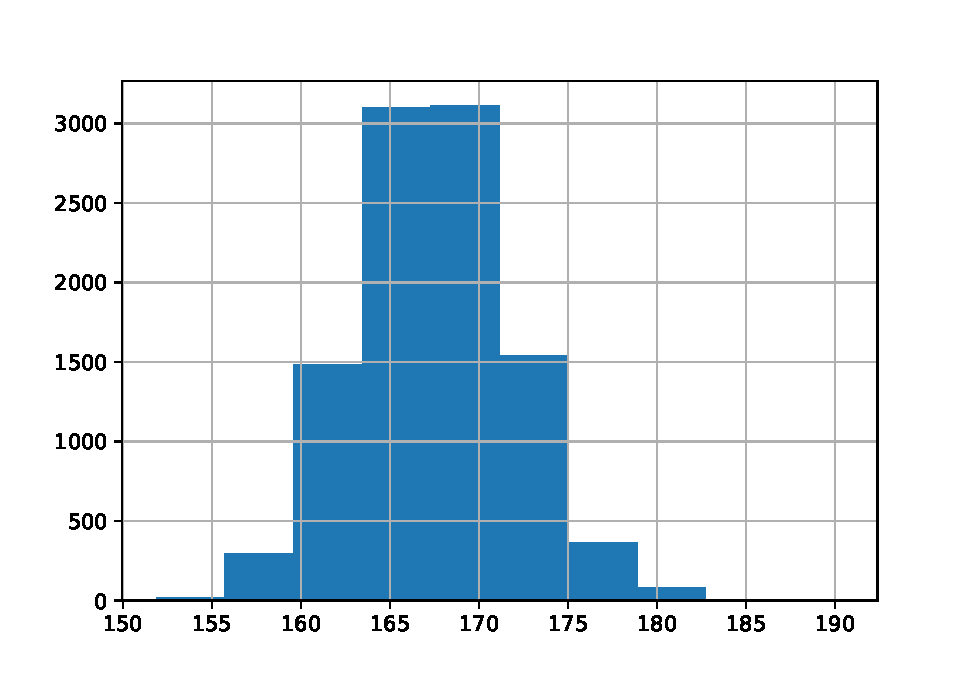
\includegraphics{_main_files/figure-latex/unnamed-chunk-259-5.pdf}

Hoppácska! Dehát, \textbf{ez itt a világ legszebb normális eloszlása!}

Ami azért második elgondolásra \textbf{teljesen logikus, mivel a Centrális Határeloszlás Tétel (CHT) dolgozik a háttérben}. Ha nem ugrik be a CHT, akkor vissza az 1. heti tananyag 2.4. fejezetéhez! :)

A \textbf{CHT} szerint ugyebár ha az \textbf{adatsor elemi véletlen hatások összegződéseként állnak elő}, akkor az \textbf{adatsor normális eloszlás}t követ. A \(\bar{y}\) \textbf{mintaátlagok adatsora pedig pont olyan adatsor, ami a CHT feltételnek megfelel!} Hiszen a mintaátlag úgy jön ki, hogy a mintaelemeket összeadom és elosztom a minta elemszámával. \textbf{Mivel a mintavétel módja FAE, így biztos lehetek benne, hogy egy mintaelem, az egy véletlen húzás, egy véletlen hatás eredménye. Aztán meg ezeket adom össze}. Végén osztok \(n\)-bel, de az mindig ugyan annyi, így nem változtat a lényegen.

Ha pedig a \textbf{sok-sok mintából számolt átlagok adatsora normális eloszlású, akkor azt is tudom, hogy milyen átlagú és milyen szórású normális eloszlást követ!}

\begin{itemize}
\tightlist
\item
  A \textbf{torzítatlanság} miatt tudom, hogy a mintaátlagok átlaga a sokasági átlag, azaz \(\mu\).
\item
  Mintaátlagok szórása pedig ugye nem más, mint a \textbf{standard hiba}, tehát \(\frac{\sigma}{\sqrt{n}}\)
\end{itemize}

Szumma szummárom, akkor a \textbf{sok-sok mintából számolt mintaátlagok \(\bar{y}\) adatsora az alábbi eloszlást követi}: \[\bar{y} \sim N\left(\mu,\frac{\sigma}{\sqrt{n}}\right)\]

Ezt az illeszkedést simán letesztelhetjük grafikusan is az 1. heti tananyag 2.3. fejezetében látott módon.
Figyeljük meg, hogy a \texttt{stats} csomag \texttt{norm.pdf} függvényében az átlagot a korábban kiszámolt \texttt{SokasagiAtlag}, a szórást pedig a szintén az előbb kiszámolt \texttt{SH} objektumok segítségével adom meg!

\begin{Shaded}
\begin{Highlighting}[]
\NormalTok{MintaVetelek100Elem.MintaAtlagok.hist(density }\OperatorTok{=} \VariableTok{True}\NormalTok{)}
\NormalTok{x\_tengely }\OperatorTok{=}\NormalTok{ np.arange(np.}\BuiltInTok{min}\NormalTok{(MintaVetelek100Elem.MintaAtlagok), np.}\BuiltInTok{max}\NormalTok{(MintaVetelek100Elem.MintaAtlagok), }\FloatTok{0.01}\NormalTok{)}
\NormalTok{y\_tengely }\OperatorTok{=}\NormalTok{ stats.norm.pdf(x }\OperatorTok{=}\NormalTok{ x\_tengely, loc }\OperatorTok{=}\NormalTok{ SokasagiAtlag, scale }\OperatorTok{=}\NormalTok{ SH)}
\NormalTok{plt.plot(x\_tengely, y\_tengely)}
\NormalTok{plt.show()}
\end{Highlighting}
\end{Shaded}

\includegraphics{_main_files/figure-latex/unnamed-chunk-260-7.pdf}

Nagyon szép, az illeszkedés, olybá tűnik a \textbf{CHT ismét működik}! :)

\section{A sokasági átlag konfidencia-intervalluma}\label{a-sokasuxe1gi-uxe1tlag-konfidencia-intervalluma}

Nézzük akkor meg \textbf{mi a valószínűsége, hogy egy véletlenszerűen kiválasztott érték egy \(N(\mu, SH)\) eloszlásban a \(\mu \pm SH\) intervallumba esik!}

\begin{Shaded}
\begin{Highlighting}[]
\NormalTok{stats.norm.cdf(x }\OperatorTok{=}\NormalTok{ SokasagiAtlag }\OperatorTok{+}\NormalTok{ SH, loc }\OperatorTok{=}\NormalTok{ SokasagiAtlag, scale }\OperatorTok{=}\NormalTok{ SH) }\OperatorTok{{-}}\NormalTok{ stats.norm.cdf(x }\OperatorTok{=}\NormalTok{ SokasagiAtlag }\OperatorTok{{-}}\NormalTok{ SH, loc }\OperatorTok{=}\NormalTok{ SokasagiAtlag, scale }\OperatorTok{=}\NormalTok{ SH)}
\end{Highlighting}
\end{Shaded}

\begin{verbatim}
## 0.6826894921370872
\end{verbatim}

Hoppáré! Ez is éppen kb. \(68\%\)! Tehát, \textbf{az, hogy egy \(\bar{y} \pm SH\) becslés csak a mintavételek \(68\%\)-ban pontos nagyjából egy valószínűségszámítási szükségszerűség}.

Kérdés, hogy \textbf{mit tehetünk ez ellen? Mihez kezdhetünk, ha mondjuk nem \(68\%\)-os, hanem valami jobb, mondjuk \(95\%\)-os megbízhatóságú intervallumbecslést szeretnénk adni a sokasági átlagra (vagy más néven sokasági várható értékre)?}

Az okoskodáshoz az 1. heti tananyag 2.6. fejezetére fogunk támaszkodni.

Ugyanis azt tudjuk, hogy ha a \textbf{mintaátlagok eloszlása} az alábbi: \[\bar{y} \sim N\left(\mu,\frac{\sigma}{\sqrt{n}}\right)\]

Akkor a \textbf{standardizált/normalizált mintaátlagok eloszlása pedig standard normális eloszlású lesz}: \[\frac{\bar{y}-\mu}{\frac{\sigma}{\sqrt{n}}} = z \sim N(0,1)\]

\textbf{Standard normális eloszlás esetén} pedig \textbf{mindig igaz}, hogy \(P(-2<z<+2) \approx 95\%\). Emlékeztetőként itt az ábra az \(N(0,1)\) standard normális eloszlás sűrűségfüggvényéről az 1. heti tananyag 2.6. fejezetéből.

\includegraphics[width=0.5\textwidth,height=\textheight]{stnormal.png}

Most az egyszerűség miatt vegyük a \(\approx\)-ot \(=\)-nek: \[P(-2<z<+2) = 95\%\]

Ebbe a \textbf{fenti összefüggésbe beírjuk a képletet, amivel kiszámoltuk \(z\)-t}: \[P\left(-2< \frac{\bar{y}-\mu}{\frac{\sigma}{\sqrt{n}}} <+2\right) = 95\%\]

Most egyelőre azzal a feltevéssel élünk, hogy ismerjük \(\sigma\)-t, azaz a sokasági szórást. Mondjuk pl. valami előzetes teljeskörű adatfelvételből. Célunk, hogy a valós, sokasági átlagot (\(\mu\)-t) foglaljuk valamiféle határok közé egy darab mintaátlag (\(\bar{y}\)) ismeretében (hiszen majd nem akarjuk mindig kivenni az összes lehetséges mintát). Tehát, az összefüggésből fejezzük a \(\mu\) sokasági átlagot: \[P\left(\bar{y}-2 \times \frac{\sigma}{\sqrt{n}}< \mu <+2 \times \frac{\sigma}{\sqrt{n}}\right) = 95\%\]

Tehát, ez a fenti összefüggés azt jelenti, hogy a \textbf{sokasági átlag az egy darab mintaátlag \(\pm 2SH\) intervallumban van kb. \(95\%\)-os valószínűséggel}. Ezt hívjuk az \textbf{átlag 95\%-os konfidencia-intervallumának}. A \(2\) pedig a \(95\%\)-os megbízhatósági szinthez tartozó \(k\) \textbf{megbízhatósági szorzó}. Mindezeket pedig csupán egy darab \(n\) elemű mintából ki is tudjuk számolni, ha \(\sigma\)-t helyettesítjük \(s\)-sel! Viszont \textbf{fontos, hogy a mintánkat véletlenszerűen válasszuk ki, mert csak így kapunk a mintaátlagok eloszlására a látott normális eloszlást!} Ugyebár a CHT-nak kellenek a véletlen kiválasztású mintaelemek a ``\emph{véletlen hatások összegződése}'' részhez.

\subsection{Az átlag konfidencia-intervallumának általános alakja}\label{az-uxe1tlag-konfidencia-intervallumuxe1nak-uxe1ltaluxe1nos-alakja}

Ha \textbf{átalánosságban akarjuk felírni ezt a konfidencia-intervallumot}, akkor úgy szoktunk fogalmazni, hogy \(1-\alpha\) \textbf{megbízhatóságú intervallum}ot írunk fel, ahol \(\alpha\) a \textbf{hibázásunk valószínűsége}, tehát, annak a valószínűsége hogy a sokasági átlag \emph{mégsem} a konfidencia-intervallumban van: \[P\left(\bar{y}-z_{1-\frac{\alpha}{2}} \times \frac{\sigma}{\sqrt{n}}< \mu <+z_{1-\frac{\alpha}{2}} \times \frac{\sigma}{\sqrt{n}}\right) = 1- \alpha\]

Itt a \(z\) érték azt akarta jelenteni, hogy azt a \(z\) \textbf{értéket kell levadászni, ami esetén az ``alá esés'' valószínűsége a standard normális eloszlásban épp} \(1-\frac{\alpha}{2}\).
Ennek okát szemlélteti az alábbi ábra.

\includegraphics[width=0.6\textwidth,height=\textheight]{normal_ci.jpg}

Ugyebár a cél az, hogy a \(z \sim N(0,1)\) eloszlásban megtaláljuk azt a \(k\) értéket, ahol \(P(-k < z < +k)=1-\alpha\). Ugyebár a \(95\%\) esetén is innen kaptuk a \(2\)-t. Ezt pedig akkor úgy kapjuk meg a \textbf{fenti ábra alapján}, hogy ha tudjuk, hogy a \(\pm k\) közé esés valószínűsége \(1- \alpha\), akkor a tartományon \textbf{kívülre esés valószínűsége} \(\alpha\), a hibázásunk megengedett valószínűsége. Ami a normális eloszlás sűrűségfüggvényének \textbf{szimmetriája miatt egyenlően oszlik el} \(-k\) alá és \(+k\) felé. Tehát a \(+k\) felé esési valószínűsége \(\alpha / 2\). De mivel a pitonban a \texttt{stats} csomag \texttt{norm.ppf} függvénye \textbf{csak ``alá esési'' valószínűségekből dolgozik}, így a \(+k\) alá esés valószínűséget kell tudnunk, ami a felé esés komplementere, azaz \(1-\frac{\alpha}{2}\), ami az \textbf{ábrán a narancssárga rész területe a sűrűségfüggvényben}.

Láthatjuk a logika szuperül működik a \(95\%\)-os megíbzhatóság, azaz \(\alpha=5\%\) esetére.

\begin{Shaded}
\begin{Highlighting}[]
\NormalTok{alfa }\OperatorTok{=} \FloatTok{0.05}

\NormalTok{stats.norm.ppf(}\DecValTok{1}\OperatorTok{{-}}\NormalTok{(alfa}\OperatorTok{/}\DecValTok{2}\NormalTok{))}
\end{Highlighting}
\end{Shaded}

\begin{verbatim}
## 1.959963984540054
\end{verbatim}

Az eredmény nem pontosan \(2\), hanem kb. \(1.96\). Ugyebár a \textbf{levezetésben kerekítettem}, de a megbízhatósági szorzó számítás lényege szerintem átjött. :)

\textbf{Szumma-szummárum}. Az \textbf{átlag tetszőleges megbízhatóságú intervallumbecslése / konfidencia-intervalluma általános alakban a következő módon számítható}: \[\bar{y} \pm k \times SH\]

Tehát, a \textbf{mintaátlagra (\(\bar{y}\)) rámérjük \(\pm\) a standard hiba \(k\)-szorosát, ahol a \(k\), mint megbízhatósági szorzó állítja be a kívánt megbízhatósági szintet}.
Ez az \textbf{általános formula azért nagyon fontos, mert a későbbiekben az átlagra vonatkozó becslések során mindig csak annyit változtatunk rajta, hogy az \(SH\) és a \(k\) mögött álló konkrét képlet fog csak változni, de ez a fenit alaplogika végig megmarad!!}

\subsection{A konfidencia-intervallum megbízhatóságának ellenőrzése}\label{a-konfidencia-intervallum-megbuxedzhatuxf3suxe1guxe1nak-ellenux151rzuxe9se}

Utolsó lépésben ellenőrizzük le konfidencia-intervallumos formulánk működését, és \textbf{nézzük meg, hogy a \(\sigma\)-val számolt \(SH\)-t használva} tudunk-e \textbf{egy \(98\%\)-os megbízhatóságú intervallumbecslés}t készíteni a Balatont átúszók időeredméyneinek átlagára a \(k=z_{1-\frac{\alpha}{2}}\) megoldásunkkal.

Tehát a \(10000\) db mintánk \textbf{mintaátlagára a mostani helyzetben} a \[\triangle = k \times SH = z_{1-\frac{\alpha}{2}} \times \frac{\sigma}{\sqrt{n}}\]

távolságot kell \(\pm\) felmérni. Ezt a \(\triangle\) távolságot hívjuk a \textbf{konfidencia-intervallum hosszának, vagy másképp a becslés teljes hibahatárának}.

Nézzük akkor meg, hogy egy \textbf{ilyen becslés tényleg kb. \(98\%\)-os találati arányt eredményez-e?}

\begin{Shaded}
\begin{Highlighting}[]
\NormalTok{n }\OperatorTok{=} \DecValTok{100}
\NormalTok{alfa }\OperatorTok{=} \DecValTok{1} \OperatorTok{{-}} \FloatTok{0.98}
\NormalTok{k }\OperatorTok{=}\NormalTok{ stats.norm.ppf(}\DecValTok{1}\OperatorTok{{-}}\NormalTok{alfa}\OperatorTok{/}\DecValTok{2}\NormalTok{)}
\NormalTok{SH }\OperatorTok{=}\NormalTok{ SokasagiSzoras }\OperatorTok{/}\NormalTok{ np.sqrt(n)}
\NormalTok{delta }\OperatorTok{=}\NormalTok{ SH }\OperatorTok{*}\NormalTok{ k}

\NormalTok{MintaVetelek100Elem[}\StringTok{\textquotesingle{}AtlagAlsoHatar\textquotesingle{}}\NormalTok{] }\OperatorTok{=}\NormalTok{ MintaVetelek100Elem[}\StringTok{\textquotesingle{}MintaAtlagok\textquotesingle{}}\NormalTok{] }\OperatorTok{{-}}\NormalTok{ delta}
\NormalTok{MintaVetelek100Elem[}\StringTok{\textquotesingle{}AtlagFelsoHatar\textquotesingle{}}\NormalTok{] }\OperatorTok{=}\NormalTok{ MintaVetelek100Elem[}\StringTok{\textquotesingle{}MintaAtlagok\textquotesingle{}}\NormalTok{] }\OperatorTok{+}\NormalTok{ delta}
\NormalTok{MintaVetelek100Elem.iloc[:,}\DecValTok{99}\NormalTok{:}\DecValTok{103}\NormalTok{]}
\end{Highlighting}
\end{Shaded}

\begin{verbatim}
##          Elem100  AtlagAlsoHatar  AtlagFelsoHatar  MintaAtlagok
## 0     165.883333      161.005186       181.518147    171.261667
## 1     128.216667      147.770020       168.282980    158.026500
## 2     215.633333      162.022353       182.535314    172.278833
## 3     112.450000      153.177686       173.690647    163.434167
## 4      99.916667      156.296353       176.809314    166.552833
## ...          ...             ...              ...           ...
## 9995  128.183333      153.425853       173.938814    163.682333
## 9996  209.300000      154.076353       174.589314    164.332833
## 9997  183.400000      153.445853       173.958814    163.702333
## 9998  196.050000      156.167353       176.680314    166.423833
## 9999  135.166667      162.793853       183.306814    173.050333
## 
## [10000 rows x 4 columns]
\end{verbatim}

Oké, akkor \textbf{megvannak az új intervallumbecsléseink} mind a \(10000\) mintára. Lássuk a pontosságukat!

\begin{Shaded}
\begin{Highlighting}[]
\NormalTok{MintaVetelekSzama }\OperatorTok{=} \BuiltInTok{len}\NormalTok{(MintaVetelek100Elem)}

\NormalTok{np.}\BuiltInTok{sum}\NormalTok{((MintaVetelek100Elem[}\StringTok{\textquotesingle{}AtlagAlsoHatar\textquotesingle{}}\NormalTok{] }\OperatorTok{\textless{}}\NormalTok{ SokasagiAtlag) }\OperatorTok{\&}\NormalTok{ (MintaVetelek100Elem[}\StringTok{\textquotesingle{}AtlagFelsoHatar\textquotesingle{}}\NormalTok{] }\OperatorTok{\textgreater{}}\NormalTok{ SokasagiAtlag)) }\OperatorTok{/}\NormalTok{ MintaVetelekSzama}
\end{Highlighting}
\end{Shaded}

\begin{verbatim}
## 0.9782
\end{verbatim}

És \textbf{tényleg kb. \(98\%\) a találati arány}, győzelem! :)

\subsection{3.3. A konfidencia-intervallum két fontos tulajdonsága}\label{a-konfidencia-intervallum-kuxe9t-fontos-tulajdonsuxe1ga}

A konfidencia-intervallum \textbf{megbízhatósági szintjével csínján kell bánni}. Ha megfigyeljük a korábbi számításainkat, akkor láthatjuk, hogy

\begin{itemize}
\tightlist
\item
  \(95\%\)-os megbízhatósághoz \(k=1.96\)
\item
  \(98\%\)-os megbízhatósághoz viszont már \(k=2.3\)
\end{itemize}

megbízhatósági szorzó tartozik.

A \(\triangle = k \times SH\) összefüggés miatt pedig könnyű látni, hogy \textbf{megbízhatósági szint növelésével a becslési hibahatár nő, azaz a konfidencia-intervallum tágul}. Teljesen logikus: ha \textbf{nagyobb találati arányt akarok, akkor ``növelni kell a hálót'', így nagyobb eséllyel akad fenn rajta a sokasági átlag}.
\(100\%\)-os megbízhatóság pedig egy esetben van, ha az intervallumbecslésünk a \(\pm \infty\) tartomány, ami ugyebár nem túl hazsnos becslési intervallum\ldots{} :)

Érdemes kipróbálni a dolgot még az \emph{1. fejezetben} kivett \(100\) elemű mintán mondjuk \(\alpha=\{0.2,0.1,0.05,0.01,0.001\}\) hibavalószínűségek mellett egy \texttt{for} ciklussal.
A számoláshoz felhasználom a korábban kiszámolt \texttt{MintaAtlag} és \texttt{SH} objektumokat.

\begin{Shaded}
\begin{Highlighting}[]
\NormalTok{alfa\_lista }\OperatorTok{=}\NormalTok{ [}\FloatTok{0.2}\NormalTok{, }\FloatTok{0.1}\NormalTok{, }\FloatTok{0.05}\NormalTok{, }\FloatTok{0.01}\NormalTok{, }\FloatTok{0.001}\NormalTok{]}

\ControlFlowTok{for}\NormalTok{ aktualis\_alfa }\KeywordTok{in}\NormalTok{ alfa\_lista:}
\NormalTok{  also\_hatar }\OperatorTok{=}\NormalTok{ MintaAtlag }\OperatorTok{{-}}\NormalTok{ SH }\OperatorTok{*}\NormalTok{ stats.norm.ppf(}\DecValTok{1}\OperatorTok{{-}}\NormalTok{aktualis\_alfa}\OperatorTok{/}\DecValTok{2}\NormalTok{)}
\NormalTok{  felso\_hatar }\OperatorTok{=}\NormalTok{ MintaAtlag }\OperatorTok{+}\NormalTok{ SH }\OperatorTok{*}\NormalTok{ stats.norm.ppf(}\DecValTok{1}\OperatorTok{{-}}\NormalTok{aktualis\_alfa}\OperatorTok{/}\DecValTok{2}\NormalTok{)}
  \BuiltInTok{print}\NormalTok{(}
    \StringTok{"Megbízhatóság: "}\OperatorTok{+}\BuiltInTok{str}\NormalTok{((}\DecValTok{1}\OperatorTok{{-}}\NormalTok{aktualis\_alfa)}\OperatorTok{*}\DecValTok{100}\NormalTok{)}\OperatorTok{+}\StringTok{"\% {-} Konf. Int.: ["}\OperatorTok{+}
    \BuiltInTok{str}\NormalTok{(}\BuiltInTok{round}\NormalTok{(also\_hatar,}\DecValTok{2}\NormalTok{))}\OperatorTok{+}\StringTok{", "}\OperatorTok{+}\BuiltInTok{str}\NormalTok{(}\BuiltInTok{round}\NormalTok{(felso\_hatar,}\DecValTok{2}\NormalTok{))}\OperatorTok{+}\StringTok{"]"}\NormalTok{)}
\end{Highlighting}
\end{Shaded}

\begin{verbatim}
## Megbízhatóság: 80.0% - Konf. Int.: [158.79, 170.09]
## Megbízhatóság: 90.0% - Konf. Int.: [157.19, 171.69]
## Megbízhatóság: 95.0% - Konf. Int.: [155.8, 173.08]
## Megbízhatóság: 99.0% - Konf. Int.: [153.08, 175.8]
## Megbízhatóság: 99.9% - Konf. Int.: [149.93, 178.95]
\end{verbatim}

Szépen megfigyelhető a leírt jelenség: \textbf{a megbízhatóság növelésével a konfidencia-intervallum egyre csak tágul, azaz a becslési hibahatár folyamatosan nő}.

\begin{itemize}
\tightlist
\item
  \(90\%\) megbízhatóság esetén az átlagos időeredményt még valahova \(157\) és \(172\) perc közé tippeljük,
\item
  \(99\%\) megbízhatóságnál viszont már \(153\) és \(176\) perc közé!
\end{itemize}

A jelenséget mérsékelni a \textbf{mintaelemszám növelésével lehet}! \textbf{Nézzük meg az előző \texttt{for} ciklust egy \(n=20\) elemű mintán az \(n=100\) helyett!} Számoljuk ki az első 20 oszlop alapján a \(\bar{y}\) mintaátlagot. Mivel a kiválasztás FAE volt, így olyan lesz a dolog, mintha csak 20 elemet választottunk volna ki a mintavétel során, nem pedig 100-at. Az \(SH=\frac{\sigma}{\sqrt{n}}\) is könnyen újraszámolható \(n=20\) mellett.

\begin{Shaded}
\begin{Highlighting}[]
\NormalTok{MintaAtlag20Elem }\OperatorTok{=}\NormalTok{ np.mean(BalcsiMinta.PERC[}\DecValTok{0}\NormalTok{:}\DecValTok{20}\NormalTok{])}
\NormalTok{n }\OperatorTok{=} \DecValTok{20}
\NormalTok{SH20Elem }\OperatorTok{=}\NormalTok{ SokasagiSzoras }\OperatorTok{/}\NormalTok{ np.sqrt(n)}

\NormalTok{alfa\_lista }\OperatorTok{=}\NormalTok{ [}\FloatTok{0.2}\NormalTok{, }\FloatTok{0.1}\NormalTok{, }\FloatTok{0.05}\NormalTok{, }\FloatTok{0.01}\NormalTok{, }\FloatTok{0.001}\NormalTok{]}

\ControlFlowTok{for}\NormalTok{ aktualis\_alfa }\KeywordTok{in}\NormalTok{ alfa\_lista:}
\NormalTok{  also\_hatar }\OperatorTok{=}\NormalTok{ MintaAtlag20Elem }\OperatorTok{{-}}\NormalTok{ SH20Elem }\OperatorTok{*}\NormalTok{ stats.norm.ppf(}\DecValTok{1}\OperatorTok{{-}}\NormalTok{aktualis\_alfa}\OperatorTok{/}\DecValTok{2}\NormalTok{)}
\NormalTok{  felso\_hatar }\OperatorTok{=}\NormalTok{ MintaAtlag20Elem }\OperatorTok{+}\NormalTok{ SH20Elem }\OperatorTok{*}\NormalTok{ stats.norm.ppf(}\DecValTok{1}\OperatorTok{{-}}\NormalTok{aktualis\_alfa}\OperatorTok{/}\DecValTok{2}\NormalTok{)}
  \BuiltInTok{print}\NormalTok{(}
    \StringTok{"Megbízhatóság: "}\OperatorTok{+}\BuiltInTok{str}\NormalTok{((}\DecValTok{1}\OperatorTok{{-}}\NormalTok{aktualis\_alfa)}\OperatorTok{*}\DecValTok{100}\NormalTok{)}\OperatorTok{+}\StringTok{"\% {-} Konf. Int.: ["}\OperatorTok{+}
    \BuiltInTok{str}\NormalTok{(}\BuiltInTok{round}\NormalTok{(also\_hatar,}\DecValTok{2}\NormalTok{))}\OperatorTok{+}\StringTok{", "}\OperatorTok{+}\BuiltInTok{str}\NormalTok{(}\BuiltInTok{round}\NormalTok{(felso\_hatar,}\DecValTok{2}\NormalTok{))}\OperatorTok{+}\StringTok{"]"}\NormalTok{)}
\end{Highlighting}
\end{Shaded}

\begin{verbatim}
## Megbízhatóság: 80.0% - Konf. Int.: [153.24, 178.5]
## Megbízhatóság: 90.0% - Konf. Int.: [149.66, 182.09]
## Megbízhatóság: 95.0% - Konf. Int.: [146.55, 185.19]
## Megbízhatóság: 99.0% - Konf. Int.: [140.48, 191.26]
## Megbízhatóság: 99.9% - Konf. Int.: [133.43, 198.31]
\end{verbatim}

Szépen láthatjuk, hogy az \textbf{átlagos átúszási időket \(99\%\)-os megbízhatósággal}

\begin{itemize}
\tightlist
\item
  \(n=20\) esetben \(140\) és \(191\) perc közé tesszük,
\item
  \(n=100\) esetben pedig láttuk az előbb, hogy a becslés pontosabb (kisebb \(\triangle\) hibahatárú): \(153\) és \(176\) perc közé teszi a sokasági átlagidőt.
\end{itemize}

Nem meglepő az eredmény. Mivel a \(\frac{\sigma}{\sqrt{n}}\) standard hiba \textbf{képlet nevezőjében van az \(n\) elemszám, így növelése csökkenti a standard hibát, ezen keresztül pedig a teljes \(\triangle\) becslési hibahatárt}. Ugyebár a 3. heti tananyagban megállapítottuk, hogy az átlag \textbf{konzisztens becslés}: elemszám növekedésével a \(SH\)-ja csökken, a \(0\)-ba tart.

Emiatt a \textbf{választott \(1-\alpha\) megbízhatósági szint a mintaelemszám függvénye}:

\begin{itemize}
\tightlist
\item
  Nagyobb \(n\) elemszám esetén egy \(99\%\)-os megbízhatóság is elég pontos intervallumbecslést szolgáltathat,
\item
  Kisebb mintaméret esetén valószínűleg meg kell elégedni valami moderáltabb (pl. \(90\%-95\%\)) megbízhatósági szinttel is.
\end{itemize}

\section{Intervallumbecslés a gyakorlatban}\label{intervallumbecsluxe9s-a-gyakorlatban}

Ezen a ponton \textbf{engedjük el a Balaton átúszókat}, és \textbf{próbáljuk ki az átlag konfidencia intervallum számítást olyan esetben, ahol nem ismerjük a teljes sokaságot, amiből mintát vettünk}.

\subsection*{1. feladat: Altatók hatékonysága}\label{feladat-altatuxf3k-hatuxe9konysuxe1ga}
\addcontentsline{toc}{subsection}{1. feladat: Altatók hatékonysága}

A sztorink a következő.

Egy gyógyszergyár egy új altató készítmény hatását vizsgálja \(10\) véletlenszerűen kiválasztott inszomniában szenvedő páciensen. Mind a tíz páciens esetében feljegyezték, hogy hány órát növekedett az alvásidejük a készítmény használatát követően. Korábbi klinikai vizsgálatok alapján ismeretes, hogy az altató készítmények által kiváltott alvásidő-változás normális eloszlású, \(2\) óra szórással.

\(Adatok = \{1.9, 0.8, 1.1, 0.1, -0.1, 4.4, 5.5, 1.6, 4.6, 3.4\}\)

Készítsünk \(95\%\)-os megbízhatósággal intervallumbecslést a várható átlagos alvásidő-változásra:

\begin{enumerate}
\def\labelenumi{\alph{enumi})}
\tightlist
\item
  a megadott feltételek alapján;
\item
  feltételezve, hogy az eloszlás normális, de a szórás ismeretlen!
\item
  Mekkora mintára van szükség, ha ugyan ekkora megbízhatóság (95\%) mellett a b) pontban kapott hibahatárt a felére kívánjuk csökkenteni?
\end{enumerate}

\subsection*{1/a) feladat megoldás}\label{a-feladat-megolduxe1s}
\addcontentsline{toc}{subsection}{1/a) feladat megoldás}

Ebben az a) feladatban nagyon el vagyunk kényeztetve. Az altató hatékonyságához van egy \(n=10\) elemű mintánk, aminek az adatait tételesen ismerjük. Első páciens alvásideje \(1.9\) órával nőtt az altató használata után, másodiké \(0.8\) órával, stb. Van egy páciens, akinek csökkent az alvásideje a gyóygszerhasználat után: az 5. delikvensé, \(0.1\) órával.
Ha ezeket az adatokat elrakjuk egy \texttt{numpy} tömbbe, akkor simán kiszámolható a megfigyelt 10 páciens esetében az átlagos alvásidő növekedés, azaz \(\bar{y}\)

\begin{Shaded}
\begin{Highlighting}[]
\NormalTok{MintaAdatok }\OperatorTok{=}\NormalTok{ np.array([}\FloatTok{1.9}\NormalTok{, }\FloatTok{0.8}\NormalTok{, }\FloatTok{1.1}\NormalTok{, }\FloatTok{0.1}\NormalTok{, }\OperatorTok{{-}}\FloatTok{0.1}\NormalTok{, }\FloatTok{4.4}\NormalTok{, }\FloatTok{5.5}\NormalTok{, }\FloatTok{1.6}\NormalTok{, }\FloatTok{4.6}\NormalTok{, }\FloatTok{3.4}\NormalTok{])}
\NormalTok{MintaAtlag }\OperatorTok{=}\NormalTok{ np.mean(MintaAdatok)}
\NormalTok{MintaAtlag}
\end{Highlighting}
\end{Shaded}

\begin{verbatim}
## 2.3299999999999996
\end{verbatim}

Tehát a megfigyelt páciensek esetében az átlagos alvásidő növekedés kb. \(\bar{y}=2.3\) óra. Ami szép és jó, de mennyi lehet az \textbf{átlagos alvásidő növekedés az inszomniás páciensek összességére, a teljes sokaságra nézve? Ehhez kell a konfidencia-intervallum! Hogy olyan betegekre is tudjunk mondani valamit, akiket a mintában NEM figyeltünk meg!}

Itt az a) esetben minden \textbf{feltételezést elfogadhatunk, amit a feladat tesz}. Ebben van egy olyan rész, ami szerint ``\emph{korábbi kutatásokból}'' ismerjük, hogy az alvásidő-változások szórása \(2\). Ha ezt így elhisszük, akkor azt mondhatjuk, hogy az alvásidő-változások teljes sokaságra vonatkozó szórását vehetjük \(2\)-nek. Azaz, \(\sigma=2\)-t ``\emph{hazudunk}'' a számolások során.
\textbf{FIGYELEM!} Ha a feladat szövege azt akarja közölni velünk, hogy van egy sokasági szórás, egy \(\sigma\), amit ismerünk és használhatunk a számolásaink során, akkor azt mindig ilyen ``\emph{korábbi kutatásokból ismeretes\ldots{}}'' szövegrészbe fogja becsomagolni!

Ha \textbf{elfogadjuk a feltételezéseinket, akkor minden adott a konfidencia-intervallum 3. fejezetben megismert képletének alkalmazásához}. Hiszen, ha \(95\%\) a megbízhatóság, akkor \(\alpha=5\%\). Tegyük is ezt: alkalmazzuk a képleteket az adatainkra!

\begin{Shaded}
\begin{Highlighting}[]
\NormalTok{n }\OperatorTok{=} \DecValTok{10}
\NormalTok{alfa }\OperatorTok{=} \DecValTok{1}\OperatorTok{{-}}\FloatTok{0.95}
\NormalTok{szigma }\OperatorTok{=} \DecValTok{2}

\NormalTok{k\_szorzo }\OperatorTok{=}\NormalTok{ stats.norm.ppf(}\DecValTok{1}\OperatorTok{{-}}\NormalTok{alfa}\OperatorTok{/}\DecValTok{2}\NormalTok{)}
\NormalTok{SH }\OperatorTok{=}\NormalTok{ szigma}\OperatorTok{/}\NormalTok{np.sqrt(n)}
\NormalTok{delta }\OperatorTok{=}\NormalTok{ k\_szorzo}\OperatorTok{*}\NormalTok{SH}

\NormalTok{also }\OperatorTok{=}\NormalTok{ MintaAtlag }\OperatorTok{{-}}\NormalTok{ delta}
\NormalTok{felso }\OperatorTok{=}\NormalTok{ MintaAtlag }\OperatorTok{+}\NormalTok{ delta}

\NormalTok{[also, felso]}
\end{Highlighting}
\end{Shaded}

\begin{verbatim}
## [1.0904099353908765, 3.5695900646091228]
\end{verbatim}

Az eredmény alapján ez az \textbf{új alatató készítmény az inszomniás páciensek teljes sokaságában a 10 elemű mintánk alapján legalább \(1.09\) óra és legfeljebb \(3.6\) óra alvásidő növekedést okoz \(95\%\)-os valószínűséggel!}

Ennek a cég vezetése nagyon örül, mert lehet olyan reklámszlogeneket elsütni az eredményünk alapján, hogy ``\emph{vizsgálatok igazolják, hogy altatónk \(95\%\)-os valószínűséggel legalább \(1\) órával növeli a várható alvásidőt}''. Egy ilyen mondat pedig minden marketinges álma \emph{úgymond}. :)

De \textbf{minden ilyen szép marad-e ha az alvásidők szórását nem a feltételezett} \(\sigma=2\)-vel, hanem a \textbf{mintából számolt korrigált szórással (\(s\)) számítjuk?}

\subsection*{1/b) feladat megoldás}\label{b-feladat-megolduxe1s}
\addcontentsline{toc}{subsection}{1/b) feladat megoldás}

Itt a feladat azt mondja, hogy ne higyjünk mindenféle kétes ``\emph{korábbi kutatásnak}'', ne fogadjuk el az általuk megadott \(\sigma\)-t, hanem \textbf{számoljunk magunknak egy korrigált mintaszórást}, azaz \(s\)-t (a korrigált mintaszórás ad torzítatlan becsést a valós, sokasági \(\sigma\)-ra), és számoljuk végig azzal a stanadard hibát \(SH=\frac{s}{\sqrt{n}}\) módon.

Viszont, ha \textbf{feloldjuk azt a feltevésünk, hogy ismerjük a sokasági szórást az \(SH\) számoláshoz} , akkor a \textbf{mintaátlagok normális helyett egy \(n-1\) szabadságfokú t-eloszlást követnek}.

A \textbf{t-eloszlás sűrűségfüggvénye az alábbi alakot ölti}. Az szabadságfokokat az angol \emph{degrees of freedom} kifejezésből \(df\)-el jelöljük.

\includegraphics[width=0.6\textwidth,height=\textheight]{studentdistr.png}

Ahogy a fenti sűrűségfüggvényből is létszik Student-féle t-eloszlás valójában egy \textbf{ellapított standard normális eloszlás} (lásd fenti ábra). A lapítás azt akarja kifejezni, hogy az eloszlás szórása nagyobb. Hiszen nagyobb szórás esetén az eloszlás szélein lévő számértékek is nagyobb valószínűséggel következhetnek be (mivel a lapítás miatt a sűrűségfüggvény magasabban fut ezeken a helyeken), így változatosabbá, jobban szóródóvá teszik az adatsorunk.

Viszont, ahogy növeljük az eloszlás szabadságfokát (\(df\)), egyre jobban ``\emph{visszacsúcsosítjuk}'' az eloszlást a standard normális eloszlásba. Logikus, hogy ilyenkor ezt az eloszlást használjuk, mivel a standard hiba értékébe (ami a mintaátlagok normális eloszlásának szórás paramétere) egy biztosan ismert sokasági szórás érték helyett, annak egy mintából számított becslését rakjuk, így \textbf{nagyobb bizonytalanságot, nagyobb szórást viszünk az eloszlásba}.

Ebben a helyzetben a konfidencia-intervallum úgy módosul, hogy \(\sigma\) helyére \(s\) kerül a \(SH\)-ban, és a \(k\) megbízhatósági szorzót \(t\)-eloszlásból számoljuk \(N(0,1)\) eloszlás helyett: \[P\left(\bar{y}-t_{1-\frac{\alpha}{2}}^{n-1} \times \frac{s}{\sqrt{n}}< \mu <+t_{1-\frac{\alpha}{2}}^{n-1} \times \frac{s}{\sqrt{n}}\right) = 1- \alpha\]

Az \(n-1\) szabadságfokú \(t\) érték számításához a \texttt{scipy} csomag \texttt{t.ppf} függvényét vesszük elő. Teljesen hasonló logikával működik, mint a \texttt{norm.ppf} függvény (vagy mint a \texttt{scipy} bármelyik eloszlás inverz értékét számoló függvénye). A \(t\)-eloszlás is szimmetrikus, tehát most is azt az értéket keressük az \(n-1\) szabadságfokú \(t\)-eloszlásunkban, ahol az ``\emph{alá esési}'' valószínűség \(1-\frac{\alpha}{2}\). A \texttt{t.ppf} függvény \texttt{df} paraméterével állítható a szabadságfok.
Ezt a mi \(n=10\) elemű mintánkra, \(95\%\)-os megbízhatósági szint mellett az alábbi módon számoljuk

\begin{Shaded}
\begin{Highlighting}[]
\NormalTok{n }\OperatorTok{=} \DecValTok{10}
\NormalTok{alfa }\OperatorTok{=} \DecValTok{1}\OperatorTok{{-}}\FloatTok{0.95}

\NormalTok{k\_szorzo\_z }\OperatorTok{=}\NormalTok{ stats.norm.ppf(}\DecValTok{1}\OperatorTok{{-}}\NormalTok{alfa}\OperatorTok{/}\DecValTok{2}\NormalTok{)}
\NormalTok{k\_szorzo\_t }\OperatorTok{=}\NormalTok{ stats.t.ppf(}\DecValTok{1}\OperatorTok{{-}}\NormalTok{alfa}\OperatorTok{/}\DecValTok{2}\NormalTok{, df }\OperatorTok{=}\NormalTok{ (n}\OperatorTok{{-}}\DecValTok{1}\NormalTok{))}

\NormalTok{[k\_szorzo\_z, k\_szorzo\_t]}
\end{Highlighting}
\end{Shaded}

\begin{verbatim}
## [1.959963984540054, 2.2621571628540993]
\end{verbatim}

Láthatjuk, hogy \textbf{a \(t\)-eloszlású \(k\) szorzó értéke érdemben nagyobb, mint a standard normális eloszlású \(k\) szorzóé ugyan arra a megengedett hibavalószínűségre}! Mivel a \(t\)-eloszlás nagyobb valószínűséget tulajdonít az extrém magas+alacsony értékek bekövetkezésének, így ha ezt alkalmazzuk, akkor ugyan ahhoz a megbízhatósági szinthez egy magasabb \(k\) megbízhatósági szorzót kapunk a \(SH\)-hoz!

Ezek után igazából csak annyi a feladatunk, hogy a teljes becslési hibahatárt kiszámítsuk \(\triangle = t_{1-\frac{\alpha}{2}}^{n-1} \times \frac{s}{\sqrt{n}}\) módon, és ezt rámérjük \(\pm\) a mintaátlagra, \(\bar{y}\)-ra. Ez már mehet ugyan úgy, mint az a) feladatban.

\begin{Shaded}
\begin{Highlighting}[]
\NormalTok{korr\_szoras }\OperatorTok{=}\NormalTok{ np.std(MintaAdatok, ddof }\OperatorTok{=} \DecValTok{1}\NormalTok{)}

\NormalTok{k\_szorzo\_t }\OperatorTok{=}\NormalTok{ stats.t.ppf(}\DecValTok{1}\OperatorTok{{-}}\NormalTok{alfa}\OperatorTok{/}\DecValTok{2}\NormalTok{, df }\OperatorTok{=}\NormalTok{ (n}\OperatorTok{{-}}\DecValTok{1}\NormalTok{))}
\NormalTok{SH }\OperatorTok{=}\NormalTok{ korr\_szoras}\OperatorTok{/}\NormalTok{np.sqrt(n)}
\NormalTok{delta }\OperatorTok{=}\NormalTok{ k\_szorzo\_t }\OperatorTok{*}\NormalTok{ SH}

\NormalTok{also }\OperatorTok{=}\NormalTok{ MintaAtlag }\OperatorTok{{-}}\NormalTok{ delta}
\NormalTok{felso }\OperatorTok{=}\NormalTok{ MintaAtlag }\OperatorTok{+}\NormalTok{ delta}

\NormalTok{[also, felso]}
\end{Highlighting}
\end{Shaded}

\begin{verbatim}
## [0.8976775393413148, 3.7623224606586847]
\end{verbatim}

Nem meglepő módon, a \textbf{t-eloszlású megbízhatósági szorzó miatt a \(95\%\)-os kinfidencia-intervallum kitágult}. Annak ellenére is, hogy az \(SH\)-ban gyakorlatilag nincs változás, mivel \(s=2.0022\). Az altató átlagos alvásidő növekedése a betegek teljes sokaságban, már \(0.9\) és \(3.76\) óra közé tehető \(95\%\)-os valószínűséggel. Szóval, ebben a reálisabb helyzetben, amikor már a szórást magunknak számoljuk a mintaadatokból, és nem pedig ``\emph{elhisszük}'' valakinek, akkor a bizonytalanság megnövekedése miatt alkalmazott t-eloszlásnak köszönhetően, a becslési hibahatár, a \(\triangle\) kitágul. A marketingesek pedig már nem mondhatnak olyan szépeket, hogy ``95\%-os valószínűséggel legalább átlag \(1\) órát növeli az alvásidőt az altató''. RIPSZ! :(

Viszont, amíg a \textbf{mintánk elemszámi kicsi}, \(n \leq 30\), addig a \textbf{t-eloszlású konfidencia intervallum számításának van egy előfeltétele: az adatsor, amiből a mintát vesszük normális eloszlású kell, hogy legyen!!}
Esetünkben ez annyit tesz, hogy az inszomniás páciensek sokaságában az \emph{alvásidő normális eloszlású} hisztogramot mutat.

Na, most itt ezt kemény \(n=10\) esetben marha nehéz értelmesen megvizsgálni a minta alapján, de lessünk egy hisztogramot a megfigyelt \(10\) db alvásidőre! A hisztogram osztályközeinek számát most nem optimalizáljuk, elfogadjuk az alapbeállításokat.

\begin{Shaded}
\begin{Highlighting}[]
\NormalTok{plt.hist(MintaAdatok)}
\NormalTok{plt.show()}
\end{Highlighting}
\end{Shaded}

\includegraphics{_main_files/figure-latex/unnamed-chunk-271-9.pdf}

Hát, a fene se tudja ennyiből eldönteni, de tényleg. Akár normális eloszlásúak lehetnek az alvásidők. :) Bízzunk a \emph{CHT}-ben: az egyéni alvásidők valószínűleg véletlen hatások összegeként állnak elő, így azok adatsora a sokaságban, a nem megfigyelt \(10\) elemű mintán \emph{kívüli} világban, lehet normális eloszlású is akár. :)

Maga a \emph{t-eloszlás} egyébként egy \emph{William Gosset} nevű angol statisztikus kreatúrája. Mr.~Gosset a \emph{Guiness} sörgyárak minőségbitosítási vezetője volt, és azt a feladatot kapta, hogy oldja meg, hogy az üveges sörök minőségbiztosítása kis mintákból is megoldható legyen. Mivel a minőségbiztosításhoz ki kell bontani az üveget és megmérni benne az összetevőket, aztán utána ezek átlagára néznek konfidencia-intervallumokat. A minőségbiztosításra kinyitott sör pedig már nem elfogyasztható. \emph{Kellemetlen}.
Így érhető, hogy minél kevesebb üvegből akarják az egész minőségbiztit megúszni. Erre adta megoldásként Gosset a t-eloszlást. Mivel a sörökben a különböző alapanyagok értéke normális eloszlást követ.

Azonban emberünk el akart büszkélkedni a saját kis elszlásával a nagy világban, ezért \emph{Student álnéven} publikálta is az eredményeit\ldots innen lett az eloszlás neve \emph{Student-féle t-eloszlás}. :) Viszont nagyon nem volt előrelátó az úriemberünk, hiszen akkoriban nyilván csak a Guiness sörgyár tudott elég kevés üvegből ugyan olyan ``jó'' megbízhatósággal minőségbiztosítani, mintha több elemű mintát vizsgáltak volna, így \emph{Mr.~Gosset} gyorsan lebukott.

Tehát, ahogy az alábbi ábra is mutatja, szegény emberünk csak a sörtermelést szerette volna hatékonyabbá tenni, de végül mindenki életét tönkretette, aki statisztikai becsléselméletet tanul. :)

\includegraphics[width=0.3\textwidth,height=\textheight]{student.png}

\subsection*{1/c) feladat megoldás}\label{c-feladat-megolduxe1s}
\addcontentsline{toc}{subsection}{1/c) feladat megoldás}

Node, térjünk vissza az altató készítményünk hatékonyságára. Ugyebár a t-eloszlással készített konfidencia-intervallum eléggé elkeserítő eredményt hozott: nem tudjuk azt mondani \(95\%\)-os megbízhatósággal, hogy készítményünk legalább \(1\) órával növeli az alvásidőt!

Mi ennek az oka? Hát a \textbf{magas becslési hiba, az átlagra épített konfidencia-intervallum hossza}, tehát a \(\triangle\). Ez most ugye nekünk \(\pm 1.43\) óra.

\begin{Shaded}
\begin{Highlighting}[]
\NormalTok{delta}
\end{Highlighting}
\end{Shaded}

\begin{verbatim}
## 1.4323224606586848
\end{verbatim}

Mondjuk ezt a becslési \textbf{hibahatárt szeretnénk levinni a felére}, \(1.43/2\), azaz kb. \(\triangle'= \pm 0.7\) órára. Ezt kétféleképpen lehet elérni. Hiszen ``\emph{magasról nézve}'', a becslési hibahatár egy kéttényezős szorzat \[\triangle=k \times SH\]

\begin{enumerate}
\def\labelenumi{\arabic{enumi}.}
\item
  Addig állítgatom a megbízhatósági-szintet, azaz valójában \(\alpha\)-t, amíg a t-eloszlásból származó \(k\) megbízhatósági szorzó olyan alacsony nem lesz, hogy az eddigi \(SH\)-val szorozgatva ki nem adja a \(0.7\)-es értéket \(\triangle\)-re. Ez az \textbf{illetlen megoldás}! Hiszen lehet, hogy ehhez az \(\alpha\)-t nagyon fel kell engedni, és a becslésnek nagyon alacsony lesz a megbízhatósága\ldots az ``\(55\%\)-os megbízhatósággal állítható az, hogy\ldots{}'' nem hangzik olyan jól marketing szempontból sem.
\item
  Az \textbf{intelligens megoldás} a mintaelemszám, azaz \(n\) növelése. Az \(\alpha\)-t adottnak vesszük, és így \(k\)-t nem bántjuk. Persze a t-eloszlás szabadságfoka miatt az elemszám \(k\)-ra is hat, de ahogy az eloszlás sűrűségfüggvényéből is látszik, kellően nagy \(n\) esetén a t-eloszlás igazából a standard normálissal lesz ekvivalens, tovább tehát nem tudjuk csökkenteni \(k\)-t adott \(\alpha\) mellett. Tehát ekkor a \(k\) lényegében fix. Ellenben \(n\) növekedése miatt az \(SH\) része a szorzatnak biztosan csökkeni fog, hiszen az átlagra konzisztens becslést adunk, tehát \(SH\) a \(0\)-ba tart \(n\) növelése esetén. Ez ugye a \(SH=\frac{s}{\sqrt{n}}\) összefüggésből adódik egyértelműen. Szóval az \(s\)-t (vagy éppen \(\sigma\)-t, ha azt ismerjük) adottnak vesszük, akkor kiszámolhatjuk, hogy mekkora \(n\) szükséges a \(\triangle'= \pm 0.7\) óra eléréséhez hibahatár fronton.
\end{enumerate}

Szóval, a 2. megoldást, az elemszám növelését választva a következő összefüggésből ki kell fejezni \(n\)-t: \[\triangle=k \times SH = z_{1-\frac{\alpha}{2}} \times \frac{s}{\sqrt{n}}\]

Hiszen \(\triangle\) helyére beírhatjuk nemes egyszerűséggel az elérni kívánt \(\triangle\)-t. A \(k\) helyére azért írtam \(z_{1-\frac{\alpha}{2}}\)-t és nem a t-eloszlású szprzót, mert a standard normális eloszlású megbízhatóságú szorzó értéke alá úgysem tudunk menni a t-eloszlással adott \(\alpha\) mellett, hiszen a t-elsozlású sűrűségfüggvényt végtelen szabadságfok mellett is csak a standard normális eloszlásba lehet maximum ``\emph{visszacsúcsosítani}'', ahogy a b) feladat megoldásában szereplő ábrán láthattuk is.

Ha pedig a fent formulából kifejeztük az elemszámot, akkor ehhez az összefüggéshez jutunk: \[n=\frac{z_{1-\frac{\alpha}{2}}^2 \times s^2}{\triangle^2}\]

Ebbe pedig gond nélkül be tudunk helyettesíteni mindent.

\begin{Shaded}
\begin{Highlighting}[]
\NormalTok{delta\_uj }\OperatorTok{=} \FloatTok{0.7}

\NormalTok{n\_uj }\OperatorTok{=}\NormalTok{ k\_szorzo\_z}\OperatorTok{**}\DecValTok{2} \OperatorTok{*}\NormalTok{ korr\_szoras}\OperatorTok{**}\DecValTok{2} \OperatorTok{/}\NormalTok{ delta\_uj}\OperatorTok{**}\DecValTok{2}
\NormalTok{n\_uj}
\end{Highlighting}
\end{Shaded}

\begin{verbatim}
## 31.429404922781128
\end{verbatim}

Tehát a becslési ha felezéséhez \(n=31.4\) elemű minta kéne\ldots{} mivel egyik betegből sem vágnánk ki \(0.4\) részt a vizsgálatra, így logikus módon az eredményt kerekítsük fel \(n=32\)-re. \textbf{Azaz, \(32-10=22\) páciensen kéne még extrában megvizsgálni az altató hatását ahhoz, hogy az átlagos alvásidő növekedést \(95\%\)-os megbízhatósággal és \(\pm0.7\) órás becslési hibával meg lehessen adni}.
Persze, ha a mintaátlag vagy éppen a korrigált mintaszórás úgy módosul az új mintaelemek hatására, hogy a konfidencia-intervallum alsó határa továbbra sem éri el a vágyott \(1\) órát, akkor tervünk dugába dőlt. Viszont, akkor ez inkább a gyógyszert fejlesztő vegyészek sara, mint a hatékonyságvizsgálatot végző statisztikusé, aki rávilágít a problémákra. :)

\subsection*{2. feladat}\label{feladat-10}
\addcontentsline{toc}{subsection}{2. feladat}

Az ESS2020.xlsx fájlban található adatbázis a 2020-ban végzett európai szociális felmérés (European Social Survey 2020 = ESS2020) 1849 magyar kitöltöjének válaszait tartalmazza 14 kérdésre (plusz van egy \emph{id} oszlop).

Ha valamelyik oszlopban üres értéket találunk, akkor az adott sorban lévő kitöltő nem válaszolt a kérdésre. Az adatbázisban szereplő kitöltők a teljes 18 év feletti magyar népességből vett véletlen mintaként kezelhetők. Most feltesszük, hogy ez a véletlen minta visszatevéses, azaz \(FAE\) is. A 6. heti tananyagban látni fogjuk, hogy ez nem is valóságtól elrugaszkodott feltevés.

Az adatbázis nyers formában eről a linkről elérhető egy ingyenes regisztráció után.

\textbf{Feladatunk} a mintavétel alapján megbecsülni, hogy hogy egy átlagos magyar polgár \(97\%\)-os megbízhatósággal várhatóan legalább és legfeljebb hány percet internetezik naponta!

\subsection*{2. feladat megoldás}\label{feladat-megolduxe1s}
\addcontentsline{toc}{subsection}{2. feladat megoldás}

Először is töltsök be az adatbázist \texttt{pandas} data frame-be és nézzük meg az elemszámot a feladat szempontjából releváns \texttt{NetUsePerDay\_Minutes} oszlopban!

\begin{Shaded}
\begin{Highlighting}[]
\NormalTok{ESS }\OperatorTok{=}\NormalTok{ pd.read\_excel(}\StringTok{"ESS2020.xlsx"}\NormalTok{)}
\NormalTok{ESS.info()}
\end{Highlighting}
\end{Shaded}

\begin{verbatim}
## <class 'pandas.core.frame.DataFrame'>
## RangeIndex: 1849 entries, 0 to 1848
## Data columns (total 15 columns):
##  #   Column                          Non-Null Count  Dtype  
## ---  ------                          --------------  -----  
##  0   id                              1849 non-null   int64  
##  1   PoliticalRadioTVPerDay_Minutes  1796 non-null   float64
##  2   NetUsePerDay_Minutes            1099 non-null   float64
##  3   TrustInParlament                1849 non-null   object 
##  4   PoliticalPartyPref              1849 non-null   object 
##  5   Education_Years                 1830 non-null   float64
##  6   WeeklyWork_Hours                685 non-null    float64
##  7   Region                          1849 non-null   object 
##  8   County                          1849 non-null   object 
##  9   SecretGroupInfluenceWorldPol    1849 non-null   object 
##  10  ScientistsDecievePublic         1849 non-null   object 
##  11  COVID19                         1849 non-null   object 
##  12  ContactCOVID19                  1849 non-null   object 
##  13  GetVaccince                     1849 non-null   object 
##  14  SomeContactCOVID19              1849 non-null   object 
## dtypes: float64(4), int64(1), object(10)
## memory usage: 216.8+ KB
\end{verbatim}

\begin{Shaded}
\begin{Highlighting}[]
\NormalTok{n }\OperatorTok{=}\NormalTok{ ESS.NetUsePerDay\_Minutes.count() }\CommentTok{\# így nem számoljuk be az üres értékeket}
\NormalTok{n}
\end{Highlighting}
\end{Shaded}

\begin{verbatim}
## 1099
\end{verbatim}

Szóval, az üres értékeket nem számolva, a releváns oszlop \texttt{count} metódusával megtudhattuk, hogy az internetezési idő esetében \(n=1099\) elemű mintából főzhetünk. \textbf{Ez bőven nagy minta}, mivel ebből a tárgyból közmegegyezéssel \textbf{az \(n > 30\) eseteket nagy mintának tekintjük}, ahogy az 1/b) feladat megoldásában megadtuk. Emiatt \textbf{nem kell az intrenetezési idők normális eloszlását sem vizsgálni az intervallumbecslés elvégzéséhez \(s\)-t és t-eloszlást használva}!

Mehetünk simán előre a \(\triangle = t_{1-\frac{\alpha}{2}}^{n-1} \times \frac{s}{\sqrt{n}}\) képletet használva.

\begin{Shaded}
\begin{Highlighting}[]
\NormalTok{n }\OperatorTok{=}\NormalTok{ ESS.NetUsePerDay\_Minutes.count() }\CommentTok{\# így nem számoljuk be az üres értékeket}

\NormalTok{minta\_atlag }\OperatorTok{=}\NormalTok{ np.mean(ESS.NetUsePerDay\_Minutes)}
\NormalTok{korr\_szoras }\OperatorTok{=}\NormalTok{ np.std(ESS.NetUsePerDay\_Minutes, ddof }\OperatorTok{=} \DecValTok{1}\NormalTok{)}

\NormalTok{SH }\OperatorTok{=}\NormalTok{ korr\_szoras }\OperatorTok{/}\NormalTok{ np.sqrt(n)}

\NormalTok{alfa }\OperatorTok{=} \DecValTok{1}\OperatorTok{{-}}\FloatTok{0.97}
\NormalTok{k\_szorzo\_t }\OperatorTok{=}\NormalTok{ stats.t.ppf(}\DecValTok{1}\OperatorTok{{-}}\NormalTok{alfa}\OperatorTok{/}\DecValTok{2}\NormalTok{, df }\OperatorTok{=}\NormalTok{ (n}\OperatorTok{{-}}\DecValTok{1}\NormalTok{))}

\NormalTok{delta }\OperatorTok{=}\NormalTok{ k\_szorzo\_t }\OperatorTok{*}\NormalTok{ SH}

\NormalTok{also }\OperatorTok{=}\NormalTok{ minta\_atlag }\OperatorTok{{-}}\NormalTok{ delta}
\NormalTok{felso }\OperatorTok{=}\NormalTok{ minta\_atlag }\OperatorTok{+}\NormalTok{ delta}

\NormalTok{[also, felso]}
\end{Highlighting}
\end{Shaded}

\begin{verbatim}
## [171.77362310362497, 190.81418399373626]
\end{verbatim}

Tehát, az \(n=1099\) elemű mintánk alapján azt mondhatjuk, hogy az átlagos magyar \(97\%\)-os megbízhatósággal legalább napi \(171.8\) percet és legfeljebb napi \(190.8\) percet tölt internetezéssel.

Az eredményünk nem nagyon változik, ha a \(k\) megbízhatósági szorzót standard normális eloszlásból számoljuk t-eloszlás helyett, hiszen az \(n\) olyan nagy, hogy az \(n-1\) szbadságfokú t-eloszlás sűrűségfüggvénye lényegében semmiben nem fog különbözni a standard normális eloszlás sűrűségfüggvényétől.

\begin{Shaded}
\begin{Highlighting}[]
\NormalTok{alfa }\OperatorTok{=} \DecValTok{1}\OperatorTok{{-}}\FloatTok{0.97}
\NormalTok{k\_szorzo\_z }\OperatorTok{=}\NormalTok{ stats.norm.ppf(}\DecValTok{1}\OperatorTok{{-}}\NormalTok{alfa}\OperatorTok{/}\DecValTok{2}\NormalTok{)}

\NormalTok{delta }\OperatorTok{=}\NormalTok{ k\_szorzo\_z }\OperatorTok{*}\NormalTok{ SH}

\NormalTok{also }\OperatorTok{=}\NormalTok{ minta\_atlag }\OperatorTok{{-}}\NormalTok{ delta}
\NormalTok{felso }\OperatorTok{=}\NormalTok{ minta\_atlag }\OperatorTok{+}\NormalTok{ delta}

\NormalTok{[also, felso]}
\end{Highlighting}
\end{Shaded}

\begin{verbatim}
## [171.785998274992, 190.80180882236922]
\end{verbatim}

Láthatjuk, hogy csak a tizedesjegyekben vannak nagyon minimális eltérések. Szóval \textbf{nagy mintaelemszám esetén a megbízhatósági szorzó nyugodtan számolható standard normális eloszlásból is a t-eloszlás helyett}.

Szerencsénkre, a \texttt{scipy} csomagban az átlag konfidencia-intervallumának számítására standard normális és t-eloszlású \(k\) szorzók esetében is \textbf{vannak beépített függvények}.
Ezek értelemszerűen \texttt{stats.norm.interval} és \texttt{stats.t.interval} nevekre hallgatnak.

\begin{itemize}
\tightlist
\item
  A függvények \texttt{scipy} paraméterében adjuk meg a \textbf{megbízhatósági szintet}, tehát NEM a ``rendes'' statisztika által \(\alpha\)-val jelölt megengedett hibavalószínűséget!!! Ezt sajnos \textbf{meg kell szokni}!!
\item
  A \texttt{loc} paraméterben érkezik a \textbf{mintaátlag}.
\item
  A \texttt{scale} paraméterbe a \textbf{standard hibát rakjuk}, ami az \textbf{adatokból közvetlenül} is számítható a \texttt{stats.sem} függvénnyel.
\item
  Csak a \texttt{stats.t.interval} esetén kell használni a \texttt{df} paramétert, ami értelemszerűen a szabadságfok helye.
\end{itemize}

Először nézzük meg, hogy tényleg használható a \texttt{stats.sem} függvény \(SH\) szmításra. A \texttt{nan\_policy\ =\ \textquotesingle{}omit\textquotesingle{}} paraméterbeállítással szólunk neki, hogy a hiányzó értékeket ne vegye figyelembe a számítás során, ahogy mi is tettük.

\begin{Shaded}
\begin{Highlighting}[]
\NormalTok{SH\_Adatokbol }\OperatorTok{=}\NormalTok{ stats.sem(ESS.NetUsePerDay\_Minutes, nan\_policy }\OperatorTok{=} \StringTok{\textquotesingle{}omit\textquotesingle{}}\NormalTok{)}

\NormalTok{[SH\_Adatokbol, SH]}
\end{Highlighting}
\end{Shaded}

\begin{verbatim}
## [4.381340690645104, 4.381340690645097]
\end{verbatim}

Egyezük, szuper! :)

Most pedig szépen használhatjuk a kétféle eloszlássa dolgozó konfidencia-intervallum számító függvényt is.

\begin{Shaded}
\begin{Highlighting}[]
\NormalTok{stats.norm.interval(}
\NormalTok{  confidence}\OperatorTok{=}\FloatTok{0.97}\NormalTok{,}
\NormalTok{  loc}\OperatorTok{=}\NormalTok{np.mean(ESS.NetUsePerDay\_Minutes),}
\NormalTok{  scale}\OperatorTok{=}\NormalTok{stats.sem(ESS.NetUsePerDay\_Minutes, nan\_policy }\OperatorTok{=} \StringTok{\textquotesingle{}omit\textquotesingle{}}\NormalTok{))}
\end{Highlighting}
\end{Shaded}

\begin{verbatim}
## (171.78599827499198, 190.80180882236925)
\end{verbatim}

\begin{Shaded}
\begin{Highlighting}[]
  
\NormalTok{stats.t.interval(}
\NormalTok{  confidence}\OperatorTok{=}\FloatTok{0.97}\NormalTok{,}
\NormalTok{  loc}\OperatorTok{=}\NormalTok{np.mean(ESS.NetUsePerDay\_Minutes),}
\NormalTok{  scale}\OperatorTok{=}\NormalTok{stats.sem(ESS.NetUsePerDay\_Minutes, nan\_policy }\OperatorTok{=} \StringTok{\textquotesingle{}omit\textquotesingle{}}\NormalTok{),}
\NormalTok{  df }\OperatorTok{=}\NormalTok{ (ESS.NetUsePerDay\_Minutes.count() }\OperatorTok{{-}} \DecValTok{1}\NormalTok{))}
\end{Highlighting}
\end{Shaded}

\begin{verbatim}
## (171.77362310362494, 190.8141839937363)
\end{verbatim}

Egyezünk a korábbi eredményeinkkel, szuperek vagyunk! :)

\section{Összefoglalás az átlag konfidencia-intervallumairól}\label{uxf6sszefoglaluxe1s-az-uxe1tlag-konfidencia-intervallumairuxf3l}

Ezen a ponton érdemes összefoglalni, hogy az átlag intervallumbecslése milyen feltételek mellett milyen konkrét formulák vannak.

Az \textbf{alapképlet a konfidencia-intervallum hosszára, azaz a becslési hibahatárra}: \[\triangle = k \times SH\]

\begin{enumerate}
\def\labelenumi{\arabic{enumi}.}
\tightlist
\item
  A sokasági szórás, alias \(\sigma\) ismert.
\end{enumerate}

\begin{itemize}
\tightlist
\item
  \(k=z_{1-\frac{\alpha}{2}}\)
\item
  \(SH=\frac{\sigma}{\sqrt{n}}\)
\end{itemize}

\begin{enumerate}
\def\labelenumi{\arabic{enumi}.}
\setcounter{enumi}{1}
\tightlist
\item
  Az adatsor, amiből a mintát vettük \emph{normális eloszlás}ú
\end{enumerate}

\begin{itemize}
\tightlist
\item
  \(k=t_{1-\frac{\alpha}{2}}^{n-1}\)
\item
  \(SH=\frac{s}{\sqrt{n}}\)
\end{itemize}

\begin{enumerate}
\def\labelenumi{\arabic{enumi}.}
\setcounter{enumi}{2}
\tightlist
\item
  A mintánk elemszáma nagy: \(n > 30\)
\end{enumerate}

\begin{itemize}
\tightlist
\item
  \(k=t_{1-\frac{\alpha}{2}}^{n-1}\) vagy \(k=z_{1-\frac{\alpha}{2}}\)
\item
  \(SH=\frac{s}{\sqrt{n}}\)
\end{itemize}

És ennyi, igazából, ha végiggondoljuk a 4. fejezet feladatait, ezt a \(3\) esetet tudjuk elkülöníteni a \(\triangle\) számítása során.

\section{Esettanulmány}\label{esettanulmuxe1ny}

Vizsgáljuk meg \(99\%\)-os megbízhatósággal hogyan alakul az átlagos internetezéssel töltött idő a teljes magyar népességben pártpreferencia szerint!

Érdekes megnézni, hogy egy \(n=1099\) elemű mintában mért átlagos különbségek az egyes pártok intenetezési idejében mennyire általánosíthatók ki a pártokat támogató népesség egészére, tehát azokra az emberekre, akiket a mintában még NEM figyeltünk meg, azaz a \textbf{mintaelemeken kívüli világra}.

Ehhez az út ott kezdődik, hogy a nominális ismérvünk, azaz a pártpreferemcia egyedi értékei szerint vesszük az átlaggal vizsgált mennyiségi ismérv részátlagait, és ezen részátlagok \(SH\)-it. Ezt a kiinduló data frame \texttt{groupby} metódusával gyorsan meg tudjuk oldani.

\begin{Shaded}
\begin{Highlighting}[]
\CommentTok{\# Először megtisztítjuk a \textquotesingle{}NetUsePerDay\_Minutes\textquotesingle{} oszlop üres értékeitől a data frame{-}t}
\NormalTok{df\_szurt }\OperatorTok{=}\NormalTok{ ESS.loc[ESS.NetUsePerDay\_Minutes.notna(),:]}

\NormalTok{PartPrefKimutatas }\OperatorTok{=}\NormalTok{ df\_szurt.groupby(}\StringTok{"PoliticalPartyPref"}\NormalTok{).agg(}
\NormalTok{  Elemszam }\OperatorTok{=}\NormalTok{ (}\StringTok{\textquotesingle{}NetUsePerDay\_Minutes\textquotesingle{}}\NormalTok{, }\StringTok{\textquotesingle{}count\textquotesingle{}}\NormalTok{),}
\NormalTok{  Atlag }\OperatorTok{=}\NormalTok{ (}\StringTok{"NetUsePerDay\_Minutes"}\NormalTok{, np.mean),}
\NormalTok{  SH }\OperatorTok{=}\NormalTok{ (}\StringTok{"NetUsePerDay\_Minutes"}\NormalTok{, stats.sem)}
\NormalTok{)}
\end{Highlighting}
\end{Shaded}

\begin{verbatim}
## <string>:2: FutureWarning: The provided callable <function mean at 0x000001CA046C13A0> is currently using SeriesGroupBy.mean. In a future version of pandas, the provided callable will be used directly. To keep current behavior pass the string "mean" instead.
\end{verbatim}

\begin{Shaded}
\begin{Highlighting}[]
\NormalTok{PartPrefKimutatas}
\end{Highlighting}
\end{Shaded}

\begin{verbatim}
##                     Elemszam       Atlag         SH
## PoliticalPartyPref                                 
## Egyesült Ellenzék        182  228.791209  12.500299
## Egyéb                     13  129.230769  20.489570
## Fidesz-KDNP              215  158.711628   8.225458
## Nem Ismert               689  176.776488   5.486396
\end{verbatim}

Ha ezzel megvagyunk, akkor nekiállhatunk kiszámolni a \(99\%\) megbízhatóságú konfidencia-intervallumokat. Az \emph{Egyéb} pártokat preferálók kivételével szép, nagy mintánk van mindenhol, így nincs nagy jelentősége, hogy \emph{t} vagy \emph{standard normális} eloszlásból számoljuk a \(k\) megbízhatósági szorzót. De mivel az \emph{Egyéb} esetben csak \(n=13\), így ott biztonságosabb, ha a magasabb \(k\)-t eredményező \(t(13-1)\) eloszlás alapján dolgozunk a konfidencia-intervallum számolásakor. Mivel a többi párt esetében ennek nincs jelentősége, így egyszerűbb az elétünk, ha a többi esetben a \(k\)-t a megfelelő \(n-1\) szabadságfokú t-eloszlásból számoljuk ki. Ezt a számolási lépést egyszerűen a \texttt{groupby}-al létrehozott data frame oszlopok bővítésével tudjuk megtenni.

\begin{Shaded}
\begin{Highlighting}[]
\NormalTok{alfa }\OperatorTok{=} \DecValTok{1}\OperatorTok{{-}}\FloatTok{0.99}

\NormalTok{PartPrefKimutatas[}\StringTok{\textquotesingle{}ci\_low\_t\textquotesingle{}}\NormalTok{] }\OperatorTok{=}\NormalTok{ PartPrefKimutatas[}\StringTok{\textquotesingle{}Atlag\textquotesingle{}}\NormalTok{] }\OperatorTok{{-}}\NormalTok{ PartPrefKimutatas[}\StringTok{\textquotesingle{}SH\textquotesingle{}}\NormalTok{] }\OperatorTok{*}\NormalTok{ stats.t.ppf(}\DecValTok{1}\OperatorTok{{-}}\NormalTok{alfa}\OperatorTok{/}\DecValTok{2}\NormalTok{, df }\OperatorTok{=}\NormalTok{ (PartPrefKimutatas[}\StringTok{\textquotesingle{}Elemszam\textquotesingle{}}\NormalTok{]}\OperatorTok{{-}}\DecValTok{1}\NormalTok{))}
\NormalTok{PartPrefKimutatas[}\StringTok{\textquotesingle{}ci\_upp\_t\textquotesingle{}}\NormalTok{] }\OperatorTok{=}\NormalTok{ PartPrefKimutatas[}\StringTok{\textquotesingle{}Atlag\textquotesingle{}}\NormalTok{] }\OperatorTok{+}\NormalTok{ PartPrefKimutatas[}\StringTok{\textquotesingle{}SH\textquotesingle{}}\NormalTok{] }\OperatorTok{*}\NormalTok{ stats.t.ppf(}\DecValTok{1}\OperatorTok{{-}}\NormalTok{alfa}\OperatorTok{/}\DecValTok{2}\NormalTok{, df }\OperatorTok{=}\NormalTok{ (PartPrefKimutatas[}\StringTok{\textquotesingle{}Elemszam\textquotesingle{}}\NormalTok{]}\OperatorTok{{-}}\DecValTok{1}\NormalTok{))}

\NormalTok{PartPrefKimutatas}
\end{Highlighting}
\end{Shaded}

\begin{verbatim}
##                     Elemszam       Atlag         SH    ci_low_t    ci_upp_t
## PoliticalPartyPref                                                         
## Egyesült Ellenzék        182  228.791209  12.500299  196.249626  261.332792
## Egyéb                     13  129.230769  20.489570   66.644566  191.816972
## Fidesz-KDNP              215  158.711628   8.225458  137.333678  180.089577
## Nem Ismert               689  176.776488   5.486396  162.605159  190.947816
\end{verbatim}

Remek! :) Ezek alapján azt mondhatjuk, hogy az egyesült ellenzék esetén egy átlagos kérdőívkitöltő \(228.8\) percet netezik naponta, míg egy átlag Fidesz kitöltő csak napi \(158.7\) percet.
Azonban, a teljes ellenzéki népességben az átlag netezési idő \(196\) és \(261\) perc között van \(99\%\)-os valószínűséggel. A teljes fideszes táborban pedig az átlagos neten töltött idő csak \(137\) és \(180\) perc között mozog, szintén \(99\%\)-os valószínűséggel.
Tehát, \(99\%\)-os valószínűséggel az átlag netezési idő az Ellenzék esetében magasabb, mint a Fidesz esetében a teljes népességben is, hiszen a ``legrosszabb'' ellenzéki átlagérték is már \(196\) perc, míg a Fidesz esetén a ``legjobb'' átlagidő is csak \(180\) perc.
Mindez persze a különböző felületeken (tv, rádió, internet) működő médiumok irányultságát figyelembe véve egyáltalán nem meglepő. :)

Ezek után telepítsünk egy \texttt{statsmodels} néven futó csomagot!

\begin{Shaded}
\begin{Highlighting}[]
\NormalTok{pip install statsmodels}
\end{Highlighting}
\end{Shaded}

A \texttt{statsmodels} csomag szépsége, hogy van egy \texttt{dot\_plot} című függvénye, amivel csudiszép vizuális megjelenítés adható a csoportátlagoknak és a konfidencia-intervallumaiknak. Ezeket az ábrákat \textbf{forest diagram}oknak hívják.

A \texttt{dot\_plot} függvény \texttt{points} paraméterébe kerülnek a mintaátlagok, míg az \texttt{intervals} paraméterbe egy olyan \(2\) oszlopos data frame kerül, ami tartalmazza a konfidencia-intervallum alsó és felső határának távolságát a mintaátlagoktól abszolút értékben, azaz lényegében a \(\triangle\)-t. Igen, itt egy olyan data frame kell neki, ahol mindkét oszlopban ugyan az az érték szerepel, mert ezt méri rá majd a gépállat a \texttt{points} paraméterre, mint egy \emph{sugár}t \(\pm\).
Ahhoz, hogy szépen megjelenjenek a pártpreferenciák is, a függvénynek a \texttt{lines} paraméteren meg kell kapnia az eredménytábla soreindexeit is, hiszen a pártpreferencia értékek ott kerültek eltárolásra.

\begin{Shaded}
\begin{Highlighting}[]
\ImportTok{from}\NormalTok{ statsmodels.graphics.dotplots }\ImportTok{import}\NormalTok{ dot\_plot}

\CommentTok{\# konfidencia{-}intervallumok méretének megadása az ábrához}
\NormalTok{intervallumok }\OperatorTok{=}\NormalTok{ np.}\BuiltInTok{abs}\NormalTok{(PartPrefKimutatas[[}\StringTok{"ci\_low\_t"}\NormalTok{, }\StringTok{"ci\_upp\_t"}\NormalTok{]] }\OperatorTok{{-}}\NormalTok{ PartPrefKimutatas[[}\StringTok{"Atlag"}\NormalTok{]].values)}

\NormalTok{dot\_plot(}
\NormalTok{  points}\OperatorTok{=}\NormalTok{PartPrefKimutatas[}\StringTok{"Atlag"}\NormalTok{],}
\NormalTok{  intervals }\OperatorTok{=}\NormalTok{ intervallumok,}
\NormalTok{  lines}\OperatorTok{=}\NormalTok{PartPrefKimutatas.index)}

\NormalTok{plt.tight\_layout() }\CommentTok{\# ne csússzanak ki a tengelyfeliratok}
\NormalTok{plt.show()}
\end{Highlighting}
\end{Shaded}

\includegraphics{_main_files/figure-latex/unnamed-chunk-282-11.pdf}

Mint láthatjuk, igazából az Ellenzék átlagos netezési ideje az, ami konfidencia-intervallumokkal együtt is magasabb, mint a többi párt szavazóinak átlagos netezési ideje a teljes népességben. Sőt, a \textbf{többi párt esetében azt mondhatjuk, hogy egyáltalán nem biztos, hogy a teljes népességben ezek az átlag netezési idők különböznek} \(99\%\)-os megbízhatósággal, \textbf{mivel a konfidencia-intervallumok metszik egymást}. Szóval, hiába van a megfigyelt adatok körében a Fidesznek magasabb átlag netideje, mint az Egyéb pártoknak, de kevesebb, mint a Nem ismert eseteknek, a nem megfigyelt, mintán kívüli adatok körében, azaz a teljes népességben simán lehet (\(99\%\)-os megbízhatósággal), hogy a Fideszes szavazók neteznek átlag a legkevesebbet egy napon. Ehhez csak annyi kell, hogy az a Fidesz valós, sokasági átlaga a konfidencia-intervallum alsó határa körül legyen a teljes népességben, míg a többi párt (nem ismert és egyéb) átlagideje pedig a konfidencia-intervallumuk tetejénél ``kössön ki'' a teljes népesség körében.

Érdemes még megfigyelni, hogy az Egyéb pártoknak a legszélesebb a konfidencia-intervalluma. Ez ugye azért van, mert mint láttuk a fejezet elején ide csak \(n=13\) kitöltő tartozik. Így az \(SH=\frac{s}{\sqrt{n}}\) összefüggés miatt érthető, hogy nagyon bizonytalanok vagyunk ennél a csoportnál az átlagos netezési idő becslésében. Ráadásul ez nem is egy teljesen pontos becslés, amit itt a konfidencia-intervallum hosszára látunk! Hiszen a kis elemszám miatt a \(k\) megbízhatósági szorzót itt \(13-1\) szabadságfokú t-eloszlásból számoltuk ki, de ehhez kellene az, hogy maguk a netezési idők normális eloszlást kövessenek. Viszont, az a helyzet, ahogy az alábbi hisztogram is szemlélteti, a napi netezési idők nem normális, hanem jobbra elnyúló eloszlásúak.

\begin{Shaded}
\begin{Highlighting}[]
\NormalTok{ESS.NetUsePerDay\_Minutes.hist()}
\NormalTok{plt.show()}
\end{Highlighting}
\end{Shaded}

\includegraphics{_main_files/figure-latex/unnamed-chunk-283-13.pdf}

\chapter{További FAE becslések és a Bootstrap módszer}\label{tovuxe1bbi-fae-becsluxe9sek-uxe9s-a-bootstrap-muxf3dszer}

\section{A Konfidencia-intervallumok két általános tulajdonsága}\label{a-konfidencia-intervallumok-kuxe9t-uxe1ltaluxe1nos-tulajdonsuxe1ga}

Az átlagra vonatkozó konfidencia-intervallumokkal kapcsolatos számolások során megállapítottunk \textbf{két olyan általános tulajdonságot a konfidencia-intervallumok hosszára, azaz a teljes becslési hibahatárra} \(\triangle\)-re vonatkozóvan, \textbf{amelyek igazak lesznek az összes többi} - a tárgyban vizsgált - \textbf{statisztikai mutató konfidencia-intervallumára} is:

\begin{enumerate}
\def\labelenumi{\arabic{enumi}.}
\tightlist
\item
  A megbízhatóság növelésével a konfidencia-intervallum egyre csak tágul, azaz a becslési hibahatár folyamatosan nő. Tehát, \textbf{nagyobb megbízhatóságú becslés csak pontatlanabb konfidencia-intervallum árán érhető el}.
\item
  Mivel a továbbiakban is konzisztensen viselkedő becslőfüggvényekkel (\(\hat{\theta}\)-kal) fogunk dolgozni, így kijelenthető, hogy a \textbf{mintaelemszám (\(n\)) növelésével}, a \(SH\) értéke csökken. A csökkenő \(SH\) miatt pedig \textbf{az egész konfidencia-intervallum pontosabb lesz}. \textbf{Magyarul} az elemszém növelésével a konfidencia-intervallum hossza, leánykori nevén \textbf{becslési hibahatár} (\(\triangle\)) \textbf{csökken}.
\end{enumerate}

A következő két fejezetben figyeljük meg, hogy \textbf{minden újabb statisztikai mutató konfidencia-intervalluma a feni két tulajdonságot betartva fog viselkedni}!

\section{Arányok konfidencia-intervalluma}\label{aruxe1nyok-konfidencia-intervalluma}

Vegyük elő újra a ESS2020.xlsx fájlban található adatbázist! Emlékeztetőül álljon itt, hogy ez az adatbázis a 2020-ban végzett európai szociális felmérés (European Social Survey 2020 = ESS2020) 1849 magyar kitöltöjének válaszait tartalmazza 14 kérdésre (plusz van egy \emph{id} oszlop).

Ugyebár az előző tananyag 4. fejezet 2. feladatában azt mondtuk, hogy ha az adatbázis valamelyik oszlopában üres értéket találunk, akkor az azt jelenti, hogy az adott sorban lévő kitöltő nem válaszolt a kérdésre. Az adatbázisban szereplő kitöltők a teljes 18 év feletti magyar népességből vett véletlen mintaként kezelhetők. Most feltesszük, hogy ez a véletlen minta visszatevéses, azaz \(FAE\) is. A következő tananyagban látni fogjuk, hogy ez nem is valóságtól elrugaszkodott feltevés.

Először is töltsök be az adatbázist ismét az Excelből egy \texttt{pandas} data frame-be és nézzük meg az \texttt{info} metódussal milyen oszlopaink (azaz ismérveink) vannak!

\begin{Shaded}
\begin{Highlighting}[]
\CommentTok{\# Elemzéshez és ábrázoláshoz szükséges csomagok betöltése}
\ImportTok{import}\NormalTok{ numpy }\ImportTok{as}\NormalTok{ np}
\ImportTok{import}\NormalTok{ pandas }\ImportTok{as}\NormalTok{ pd}
\ImportTok{import}\NormalTok{ matplotlib.pyplot }\ImportTok{as}\NormalTok{ plt}
\ImportTok{import}\NormalTok{ scipy.stats }\ImportTok{as}\NormalTok{ stats}
\ImportTok{from}\NormalTok{ statsmodels.stats.meta\_analysis }\ImportTok{import}\NormalTok{ combine\_effects}
\ImportTok{from}\NormalTok{ statsmodels.graphics.dotplots }\ImportTok{import}\NormalTok{ dot\_plot}

\CommentTok{\# Adatbeolvasás data frame{-}be}
\NormalTok{ESS }\OperatorTok{=}\NormalTok{ pd.read\_excel(}\StringTok{"ESS2020.xlsx"}\NormalTok{)}
\NormalTok{ESS.info()}
\end{Highlighting}
\end{Shaded}

\begin{verbatim}
## <class 'pandas.core.frame.DataFrame'>
## RangeIndex: 1849 entries, 0 to 1848
## Data columns (total 15 columns):
##  #   Column                          Non-Null Count  Dtype  
## ---  ------                          --------------  -----  
##  0   id                              1849 non-null   int64  
##  1   PoliticalRadioTVPerDay_Minutes  1796 non-null   float64
##  2   NetUsePerDay_Minutes            1099 non-null   float64
##  3   TrustInParlament                1849 non-null   object 
##  4   PoliticalPartyPref              1849 non-null   object 
##  5   Education_Years                 1830 non-null   float64
##  6   WeeklyWork_Hours                685 non-null    float64
##  7   Region                          1849 non-null   object 
##  8   County                          1849 non-null   object 
##  9   SecretGroupInfluenceWorldPol    1849 non-null   object 
##  10  ScientistsDecievePublic         1849 non-null   object 
##  11  COVID19                         1849 non-null   object 
##  12  ContactCOVID19                  1849 non-null   object 
##  13  GetVaccince                     1849 non-null   object 
##  14  SomeContactCOVID19              1849 non-null   object 
## dtypes: float64(4), int64(1), object(10)
## memory usage: 216.8+ KB
\end{verbatim}

Láthatjuk, hogy megvan mind a 14+1 oszlopunk a megfelelő adattípusokkal. Hurrá! :)

\textbf{Feladatunk} ezúttal az lenne, hogy \textbf{99\%-os megbízhatóságú konfidencia-intervallum}ot építsünk a \textbf{Fideszt támogatók arányára!}

Szerencsére ezt aránylag könnyű megtenni, hiszen \textbf{egy adott tulajdonsággal bíró egyedek aránya lényegében egy átlag}! Konkrétan \textbf{egy olyan változó átlaga, ahol a tulajdonsággal bíró egyedek \(1\) értéket, míg a tulajdonsággal NEM rendelkező egyedek \(0\) értéket kapnak}.

Ezt könnyű is szemléltetni Python-ban. Vegyük a feladat szempontjából releváns a \texttt{PoliticalPartyPref} ismérv \textbf{relatív gyakoriságait} a \texttt{value\_counts} metódus segítségével:

\begin{Shaded}
\begin{Highlighting}[]
\CommentTok{\# Teljes mintaelemszám megadása}
\NormalTok{n }\OperatorTok{=}\NormalTok{ ESS.PoliticalPartyPref.count()}

\CommentTok{\# Relatív Gyakoriságok}
\NormalTok{ESS.PoliticalPartyPref.value\_counts() }\OperatorTok{/}\NormalTok{ n}
\end{Highlighting}
\end{Shaded}

\begin{verbatim}
## PoliticalPartyPref
## Nem Ismert           0.643050
## Fidesz-KDNP          0.197404
## Egyesült Ellenzék    0.148729
## Egyéb                0.010817
## Name: count, dtype: float64
\end{verbatim}

Ez alapján ugye a Fidesz támogatóinak aránya a megfigyelt 1849 elemű mintában \(19.7\%\). Ezt az eredményt pedig úgy is megkaphatjuk, hogy csinálunk egy új \texttt{Fidesz} nevű oszlopot az \texttt{ESS} nevű data frame-be, amiben a Fidesz támogatók \(1\) értéket kapnak, a többiek \(0\)-t, és vesszük az új oszlop átlagát.
Az új oszlop létrehozásához a \texttt{numpy} csomag \texttt{where} néven futó függvényét használjuk. Ez lényegében olyan, mint az Excel \texttt{HA} függvénye: egy logikai feltétel megadása után értéket adunk az új oszlopban a \emph{feltétel igaz} ágon, majd utána a \emph{feltétel hamis} ágon.

\begin{Shaded}
\begin{Highlighting}[]
\CommentTok{\# Létrehozzuk a Fidesz nevű oszlopot!}
\NormalTok{ESS[}\StringTok{\textquotesingle{}Fidesz\textquotesingle{}}\NormalTok{] }\OperatorTok{=}\NormalTok{ np.where(ESS.PoliticalPartyPref}\OperatorTok{==}\StringTok{\textquotesingle{}Fidesz{-}KDNP\textquotesingle{}}\NormalTok{, }\DecValTok{1}\NormalTok{, }\DecValTok{0}\NormalTok{)}

\CommentTok{\# És vesszük az új oszlop átlagát}
\NormalTok{np.average(ESS.Fidesz)}
\end{Highlighting}
\end{Shaded}

\begin{verbatim}
## 0.19740400216333154
\end{verbatim}

Ismét megkaptuk a \(19.7\%\)-os támogatottsági arányt. Ez alapján pedig könnyen elkészíthetjük rá a 99\%-os megíbzhatóságú konfidencia-intervallumot a \texttt{scipy} csomag \texttt{stats.norm.interval} függvényével. Hiszen a nagy mintaelemszám miatt nem szükséges a \(k\) szorzót t-eloszlásból számolni, bőven megfelel nekünk a standard normális eloszlás alkalmazása is.

\begin{Shaded}
\begin{Highlighting}[]
\NormalTok{stats.norm.interval(}
\NormalTok{  confidence}\OperatorTok{=}\FloatTok{0.99}\NormalTok{,}
\NormalTok{  loc}\OperatorTok{=}\NormalTok{np.mean(ESS.Fidesz),}
\NormalTok{  scale}\OperatorTok{=}\NormalTok{stats.sem(ESS.Fidesz, nan\_policy }\OperatorTok{=} \StringTok{\textquotesingle{}omit\textquotesingle{}}\NormalTok{))}
\end{Highlighting}
\end{Shaded}

\begin{verbatim}
## (0.1735537723743666, 0.2212542319522965)
\end{verbatim}

Tehát, a mintánk alapján a \textbf{magyar népesség egészét tekintve az mondható el, hogy 99\%-os valószínűséggel legalább \(17.4\%\)-uk támogatja a Fidesz-KDNP-t, viszont szintén 99\%-os valószínűséggel kijelenthető, hogy a támogatottsági arányuk nem magasabb \(22.1\%\)-nál}.

A teljes népességre nézve vett Fidesz támogatottság vizsgálható a \texttt{statsmodels} csomag \texttt{combine\_effects} függvényével \textbf{regionális bontásban} is.

Mielőtt a \texttt{combine\_effects} függvényt használnánk, csináljuk meg a kiinduló kimutatást az \texttt{ESS} data frame \texttt{groupby} metódusával:

\begin{enumerate}
\def\labelenumi{\arabic{enumi}.}
\tightlist
\item
  A nominális ismérvünk, azaz most a \texttt{Region} egyedi értékei szerint vesszük az átlaggal vizsgált mennyiségi ismérv (most \texttt{Fidesz}) részátlagait
\item
  Utána ezen részátlagok \(SH^2\)-eit, azaz \emph{becslési varianciáit} is megadjuk.
\end{enumerate}

\begin{Shaded}
\begin{Highlighting}[]
\NormalTok{RegionKimutatas }\OperatorTok{=}\NormalTok{ ESS.groupby(}\StringTok{"Region"}\NormalTok{).agg(}
\NormalTok{  Elemszam }\OperatorTok{=}\NormalTok{ (}\StringTok{\textquotesingle{}Fidesz\textquotesingle{}}\NormalTok{, }\StringTok{\textquotesingle{}count\textquotesingle{}}\NormalTok{),}
\NormalTok{  Atlag }\OperatorTok{=}\NormalTok{ (}\StringTok{"Fidesz"}\NormalTok{, np.mean),}
\NormalTok{  SH }\OperatorTok{=}\NormalTok{ (}\StringTok{"Fidesz"}\NormalTok{, stats.sem)}
\NormalTok{)}
\end{Highlighting}
\end{Shaded}

\begin{verbatim}
## <string>:1: FutureWarning: The provided callable <function mean at 0x000001CA046C13A0> is currently using SeriesGroupBy.mean. In a future version of pandas, the provided callable will be used directly. To keep current behavior pass the string "mean" instead.
\end{verbatim}

\begin{Shaded}
\begin{Highlighting}[]
\CommentTok{\# SH négyzetre emelés}
\NormalTok{RegionKimutatas[}\StringTok{\textquotesingle{}BecslesiVar\textquotesingle{}}\NormalTok{] }\OperatorTok{=}\NormalTok{ RegionKimutatas[}\StringTok{\textquotesingle{}SH\textquotesingle{}}\NormalTok{]}\OperatorTok{**}\DecValTok{2}

\NormalTok{RegionKimutatas}
\end{Highlighting}
\end{Shaded}

\begin{verbatim}
##                     Elemszam     Atlag        SH  BecslesiVar
## Region                                                       
## Budapest                 298  0.248322  0.025069     0.000628
## Dél-Alföld               167  0.125749  0.025734     0.000662
## Dél-Dunántúl             143  0.153846  0.030278     0.000917
## Közép-Dunántúl           242  0.219008  0.026641     0.000710
## Nyugat-Dunántúl          221  0.167421  0.025171     0.000634
## Pest                     265  0.222642  0.025604     0.000656
## Észak-Alföld             305  0.144262  0.020152     0.000406
## Észak-Magyarország       208  0.264423  0.030653     0.000940
\end{verbatim}

Látható, hogy a mintán belül a Fidesz támogatottsága az Dél-Dunántúlon csak 15.4\%, míg Nyugat-Dunántúlon 16.7\%. Kérdés, hogy ezek a különbségek a mintavételi hiba, azaz a 99\%-os megbízhatóságú konfidencia-intervallum figyelembe vételével is megmaradnak-e!

Ami fontos még az előbb elkészített kimutatásból, hogy \textbf{minden régióban megvan a nagy elemszám} (\(n>30\)), így nyugodtan használható a \(k\) megbízhatósági szorzót standard normális eloszlásból számító \texttt{combine\_effects} függvény. A függvény paraméterezési szabályait lásd a 4. heti tananyag 6. fejezetében.

\begin{Shaded}
\begin{Highlighting}[]
\NormalTok{eredmeny }\OperatorTok{=}\NormalTok{ combine\_effects(}
\NormalTok{  effect }\OperatorTok{=}\NormalTok{ RegionKimutatas.Atlag,}
\NormalTok{  variance }\OperatorTok{=}\NormalTok{ RegionKimutatas.BecslesiVar,}
\NormalTok{  row\_names }\OperatorTok{=}\NormalTok{ RegionKimutatas.index,}
\NormalTok{  alpha }\OperatorTok{=}\NormalTok{ (}\DecValTok{1}\OperatorTok{{-}}\FloatTok{0.99}\NormalTok{)}
\NormalTok{)}

\CommentTok{\# a summary\_frame eredményéból az első 8 sor kell nekünk,}
\CommentTok{\# mert 8 régió szerint vizsgáljuk a támogatottsági arányokat!}
\NormalTok{eredmeny\_tabla }\OperatorTok{=}\NormalTok{ eredmeny.summary\_frame().iloc[}\DecValTok{0}\NormalTok{:}\DecValTok{8}\NormalTok{,}\DecValTok{0}\NormalTok{:}\DecValTok{4}\NormalTok{]}
\NormalTok{eredmeny\_tabla}
\end{Highlighting}
\end{Shaded}

\begin{verbatim}
##                          eff    sd_eff    ci_low    ci_upp
## Budapest            0.248322  0.025069  0.199187  0.297457
## Dél-Alföld          0.125749  0.025734  0.075310  0.176187
## Dél-Dunántúl        0.153846  0.030278  0.094503  0.213189
## Közép-Dunántúl      0.219008  0.026641  0.166794  0.271223
## Nyugat-Dunántúl     0.167421  0.025171  0.118086  0.216756
## Pest                0.222642  0.025604  0.172458  0.272825
## Észak-Alföld        0.144262  0.020152  0.104766  0.183759
## Észak-Magyarország  0.264423  0.030653  0.204344  0.324503
\end{verbatim}

Az eredményül kapott táblából ismételten látható, hogy a \textbf{mintán belül a Fidesz támogatottsága az Dél-Alföldön csak 12.6\%, míg Dél-Dunántúlon már 15.4\%}. Azonban, ha a konfidencia-intervallum segítségével a \textbf{teljes népességet vizsgáljuk, akkor ez 99\%-os valószínűséggel egy NEM szignifikáns} (jelentős) \textbf{eltérés, mivel a két konfidencia-intervallum metszi egymást!} Tehát a teljes népességben elképzelhető legjobb esetben egy 17.6\%-os támogatottság is a Dél-Alföldön, míg a legrosszabb esetben belefér a Dél-Dunántúlon 9.5\%-os támogatottság is. Tehát, az, hogy a Dél-Dunántúlon magasabb a Fidesz támogatottsági arány a mintában, az lehet csak a mintavételi hiba műve 99\%-os megbízhatósággal! Ellenben az \textbf{Észak-Magyarországi Fidesz támogatottság 99\% valószínűséggel a sokaságban is magasabb, mint a Dél-Alföldi}, hiszen a Dél-Alföldön a támogatottság legjobb esetben is csak 17.6\%, míg Észak-Magyarországon legrosszabb esetben is már 20.4\%. Tehát a \textbf{két konfidencia-intervallum NEM metszi egymást, a mintában mért eltérések 99\% valószínűséggel megmaradnak a sokaságban is!}

Az eredményekről ugyan úgy készíthetünk \textbf{forest diagram}ot, mint a pártpreferenciák szerint bontott átlagos netezési időkről a 4. heti tananyag 6. fejezetében. Itt ugyebár a \texttt{statsmodels} csomag \texttt{dot\_plot} függvényét vetjük be. Ennek a használatáról is bővebb információk a 4. heti tananyag 6. fejezetében találhatók.

\begin{Shaded}
\begin{Highlighting}[]
\CommentTok{\# konfidencia{-}intervallumok méretének megadása az ábrához}
\NormalTok{intervallumok }\OperatorTok{=}\NormalTok{ np.}\BuiltInTok{abs}\NormalTok{(eredmeny\_tabla[[}\StringTok{"ci\_low"}\NormalTok{, }\StringTok{"ci\_upp"}\NormalTok{]] }\OperatorTok{{-}}\NormalTok{ eredmeny\_tabla[[}\StringTok{"eff"}\NormalTok{]].values)}
\NormalTok{intervallumok}
\end{Highlighting}
\end{Shaded}

\begin{verbatim}
##                       ci_low    ci_upp
## Budapest            0.049135  0.049135
## Dél-Alföld          0.050439  0.050439
## Dél-Dunántúl        0.059343  0.059343
## Közép-Dunántúl      0.052215  0.052215
## Nyugat-Dunántúl     0.049335  0.049335
## Pest                0.050183  0.050183
## Észak-Alföld        0.039496  0.039496
## Észak-Magyarország  0.060080  0.060080
\end{verbatim}

\begin{Shaded}
\begin{Highlighting}[]
\CommentTok{\# ábra elkészítése}
\NormalTok{dot\_plot(}
\NormalTok{  points}\OperatorTok{=}\NormalTok{eredmeny\_tabla[}\StringTok{"eff"}\NormalTok{],}
\NormalTok{  intervals }\OperatorTok{=}\NormalTok{ intervallumok,}
\NormalTok{  lines}\OperatorTok{=}\NormalTok{eredmeny\_tabla.index)}

\CommentTok{\# ábra megjelenítése}
\NormalTok{plt.tight\_layout() }\CommentTok{\# ne csússzanak ki a tengelyfeliratok}
\NormalTok{plt.show()}
\end{Highlighting}
\end{Shaded}

\includegraphics{_main_files/figure-latex/unnamed-chunk-290-15.pdf}

Az előbb taglalt, 99\%-os megbízhatósággal a sokaságban is szignifikáns eltérés Dél-Alföld és Észak-Magyarország között. Az is látszik, hogy \textbf{hasonló szignifikáns különbség még} ezen kívül \textbf{Dél-Alföld és Budapest Fidesz támogatottsági aránya között található}.

\subsection{Mintaelemszám meghatározása aránybecsléshez}\label{mintaelemszuxe1m-meghatuxe1rozuxe1sa-aruxe1nybecsluxe9shez}

Érdemes az arány konfidencia-intervallumának számítása során felhasználni azt az információt, hogy egy csak 0-ból és 1-ből álló változó korrigált mintaszórása \(s=\sqrt{p(1-p)}\) módon számítható, ahol \(p\) az \(1\) értékek aránya a mintában!
Nézzük is meg, hogy igaz-e ez! Ugyebár a Fidesz támogatottsági aránya a teljes 1849 elemű mintában \(p=19.7\%\). Ez alapján a szórása a \texttt{Fidesz} nevű 0-1-ből álló változónak \(s=\sqrt{p(1-p)}=\sqrt{0.197 \times (1-0.197)}=0.3977323\).

Nézzük meg az eredményt a \texttt{numpy} csomag \texttt{std} függvényével is:

\begin{Shaded}
\begin{Highlighting}[]
\NormalTok{np.std(ESS.Fidesz)}
\end{Highlighting}
\end{Shaded}

\begin{verbatim}
## 0.3980397745115843
\end{verbatim}

A kétféleképp számolt érték némi kerekítési hibát leszámítva egyezik! :) De hát ez nem meglepő, hogy így alakult, hiszen a 3. heti tananyag 5. fejezetében éppen azt mondtuk, hogy a mintaarányok (a \(p\)-k) standard mintavételi hibája a \(SH(p) \approx \sqrt{\frac{p(1-p)}{n}}\) képlettel megadható. :)

Ez azt jelenti, hogy \textbf{az arány konfidencia-intervallumának hossza} a \(\triangle = SH \times k\) képlet alapján \(\sqrt{\frac{p(1-p)}{n}} \times k\) módon számítható, hiszen az átlag standard hibája \(\frac{s}{\sqrt{n}}\) volt, és most felhasználtuk, hogy csak 0-1-et tartalmazó változókra \(s=\sqrt{p(1-p)}\). A \(k\) megbízhatósági szorzó pedig ugyan úgy \(N(0,1)\) eloszlással számolható \emph{nagy méretű minták esetén}, mint az átlag konfidencia-intervallumánál. Hiszen magas \(n\) esetén a \(t(n-1)\) eloszlás sűrűségfüggvénye már lényegében egybeesik az \(N(0,1)\) eloszlás sűrűségfüggvényével, ahogy a 4. heti tananyag 4. fejezetének 2. feladatában is láttuk.

\textbf{Ennyi információ alapján pedig képesek vagyunk arra, hogy még mintavétel ELŐTT meghatározzuk, hogy az arány egy adott pontosságú és megbízhatóságú becsléséhez mekkora elemszámú mintára van szükségünk}.

Hiszen \(99\%\)-os megbízhatósági szint mellett a szükséges megbízhatósági \(k\) szorzó a standard normális, azaz \(N(0,1)\) eloszlás inverz értéke alapján megadható \(z_{1-\frac{\alpha}{2}}\) módon:

\begin{Shaded}
\begin{Highlighting}[]
\NormalTok{alfa}\OperatorTok{=}\DecValTok{1}\OperatorTok{{-}}\FloatTok{0.99}
\NormalTok{stats.norm.ppf(}\DecValTok{1}\OperatorTok{{-}}\NormalTok{alfa}\OperatorTok{/}\DecValTok{2}\NormalTok{)}
\end{Highlighting}
\end{Shaded}

\begin{verbatim}
## 2.5758293035489004
\end{verbatim}

Vegyük az értéket kerekítve \(k=2.6\)-nak!

Ugyebár azt tudjuk, hogy a jelenlegi 1849 elemű mintánk esetén Fidesz támogatottsági aránya \(p=19.7\%\), \textbf{amitől a támogatottsági arány valós sokasági értéke} 99\%-os valószínűséggel \(\pm\) \textbf{2.4 százalékpontos hibahatárral térhet el}: \[\pm \triangle = SH \times k = \sqrt{\frac{p(1-p)}{n}} \times k = \sqrt{\frac{0.197 \times (1-0.197)}{1849}} \times 2.6=0.0240\]

De mi a helyzet, ha a \textbf{hibahatár értékét 1 százalékpontra akarom csökkenteni és meg akarom őrizni a 99\%-os megízhatósági szintet}? Ekkor \textbf{nagyobb mintát kell venni, kérdés, hogy mennyivel nagyobbat}. Ezek alapján a kívánt \(\triangle\) érték \(0.01\) és a \(k=2.6\) értékből sem akarok engedi. Azaz: \[0.01 = \sqrt{\frac{p(1-p)}{n}} \times 2.6\]

Ebből \(n\)-t kifejezve: \[n=\frac{2.6^2 \times p(1-p)}{0.01^2}\]

Ezen a ponton nagy a csábítás, hogy a képletből úgy számoljuk ki \(n-t\), hogy \(p=19.7\%\)-kal dolgozzunk. De ezt \textbf{ne tegyük}! Mivel nem tudjuk, hogy a megnövelt elemszámú mintában mennyi is lesz \(p\). Plusz, ha a \textbf{szükséges mintaelemszámot AZELŐTT akarjuk meghatározni, hogy a kérdéses \(p\) arány becslésére már vettünk mintát, akkor aztán tényleg lövésünk nincs a \(p\) értékéről}!

Szerencsére, \textbf{rájöhetünk, hogy a \(p(1-p)\) kifejezésnek könnyen meg tudjuk adni a maximumát}, hiszen az \(f(p)=p(1-p)=p-p^2\) függvény egy fordította parabola, melynek maximuma \(p=0.5\)-nél kerül felvételre és értéke \(max(p(1-p))=0.25\):

\includegraphics[width=0.5\textwidth,height=\textheight]{p_SH.jpg}

Szóval az \(N=\frac{2.6^2 \times p(1-p)}{0.01^2}\) formulába \textbf{mindig beírhatjuk a \(0.25\)-öt, hiszen ez a legrosszabb szituációnk, ekkor lesz aránybecslés esetén maximális a standard hibánk}. Ha elégség nagy mintát veszünk, hogy a maximális \(SH\) mellett is \(\triangle = 0.01\)-et érjünk el, akkor minden egyéb esetben is jók vagyunk.

Tehát, \textbf{az 1 százalékpontos hibahatár eléréséhez szükséges elemszám 99\%-os megbízhatóság mellett} \(N=\frac{2.6^2 \times 0.25}{0.01^2}=16900\) \textbf{fő}.
Ennek fényében különsöen érdekes meglesni \href{https://ig.ft.com/sites/brexit-polling/}{ezen a linken} hogy hány fős mintából dolgoztak a 2016-os Brexit népszavazás eredményének előrejelzése során a közvéleménykutatók, ahol lehetett tudni, hogy nagyon kiélezett a verseny a maradás és elszakadás pártok között, így a két párt támogatottsági arányának becslése során \textbf{nagyon szükség lett volna erre az 1 százalékpontos hibahatárra és a 99\%-os megbízhatósági szintre, ami a 16900 elemű minták biztosítanak arányok becslése során}.

További érdekes példaként vegyük a Momentum Mozgalom 2021. október 11-én megosztott plakátját:

\includegraphics[width=0.45\textwidth,height=\textheight]{Momo Mintavételi hiba.jpg}

Ha megnézzük a kép jobb alsó sarkát láthatjuk, hogy az adatok forrása a Medián közvélemény kutató intézet. A dátum alapján rájöhetünk, hogy \href{https://hvg.hu/itthon/20211011_Median_MarkiZay_elonyhoz_juttathatja_az_ellenzeket}{erről a Medián közvéleménykutatásról szól a plakát}. A linkelt HVG cikkből megtudhatjuk, hogy a Medián közvéleménykutatása egy \(n=1000\) elemű véletlen mintát takar. Ebben az esetben számoljuk ki a különböző pártlisták támogatottsági arányaihoz a maximális \(\triangle\) hibahatárt, azaz vegyük \(p(1-p)\)-t \(0.25\)-nek:\[\pm \triangle = SH \times k = \sqrt{\frac{p(1-p)}{n}} \times k = \sqrt{\frac{0.25}{1000}} \times 2.6=0.0411\]

Tehát a hibahatár durván \textbf{4 százalékpont}. Ha ezt az értéket Dobrev Klára esetén levonjuk a Fidesz támmogatottsági arányából és hozzáadjuk az Ellenzék témogatottsági arányához, majd ha MZP esetén az Ellenzéki arányból levonjuk és a Fideszhez hozzáadjuk, akkor láthatjuk, hogy \textbf{a plakáton kimutatott Fidesz és Ellenzéki pártlisták támogatottsági arányai közötti különbség MZP és Dobrev esetén is bőven a mintavételi hibahatáron belül van}!
Tehát, egyik esetben sem mondható el a konfidencia-intervallum alapján, hogy a teljes népességben reális lenne a plakát állítása, miszerint csak MZP-vel verhető a Fidesz. Az \textbf{plakát üzenete csak a megfigyelt 1000 elemű mintán belül vehető igaznak}! Amit meg is erősít a 2022-es országgyűlési választások eredménye\ldots{}

\subsection{Szükséges minimális elemszám aránybecsléshez}\label{szuxfcksuxe9ges-minimuxe1lis-elemszuxe1m-aruxe1nybecsluxe9shez}

Az \textbf{arány intervallumbecslés} esetén \textbf{van} a 2.1. fejezetben taglaltak mellett egy \textbf{minimális elemszám követelménye is, aminél kisebb mintákban az intervallumbecslés egyáltalán NEM elvégezhető!!}

Ez a követelemény abból jön, hogy az aránybecslést gyakorlatilag egy átlagbecslésre vezetjük vissza.
Hiszen átlagbecslés esetén \textbf{kis elemszámú mintáknál feltételezzük az alapsokaság} (tehát, amiből a mintát vettük) \textbf{normális eloszlását, még akkor is, ha a megbízhatósági szorzót t-eloszlásból számítjuk!} Egy \textbf{csak \(0\)-ból és \(1\)-ből álló adatsor pedig bajosan fog normális eloszlást követni!} :)

Azt, hogy \textbf{mi számít aránybecslés esetén nagy mintának, a következő szabály adja meg}:

\begin{itemize}
\tightlist
\item
  Legyen az arány szempontjából \emph{kedvező} esetek száma több, mint 10 a mintában, azaz: \(n \times p >10\)
\item
  Legyen az arány szempontjából \emph{kedvezőtlen} esetek száma is több, mint 10 a mintában, azaz: \(n \times (1-p) >10\)
\end{itemize}

Ez a Fidesz támogatók arányának korűábbi példájára nézve úgy néz ki, hogy a teljes mintánk elemszáma \(n=1849\) fő:

\begin{Shaded}
\begin{Highlighting}[]
\BuiltInTok{len}\NormalTok{(ESS) }\CommentTok{\# tábla sorainak száma}
\end{Highlighting}
\end{Shaded}

\begin{verbatim}
## 1849
\end{verbatim}

Míg az arány szempontjából \emph{kedvező} esetek, azaz a Fidesz-KDNP támogatók száma \(365\) fő:

\begin{Shaded}
\begin{Highlighting}[]
\NormalTok{ESS.loc[ESS[}\StringTok{\textquotesingle{}PoliticalPartyPref\textquotesingle{}}\NormalTok{] }\OperatorTok{==} \StringTok{\textquotesingle{}Fidesz{-}KDNP\textquotesingle{}}\NormalTok{, }\StringTok{\textquotesingle{}PoliticalPartyPref\textquotesingle{}}\NormalTok{].count()}
\end{Highlighting}
\end{Shaded}

\begin{verbatim}
## 365
\end{verbatim}

Tehát a \textbf{két feltétel itt a következőképpen teljesül}:

\begin{itemize}
\tightlist
\item
  A \emph{kedvező} esetek száma \(365 > 10 \rightarrow\) \textbf{feltétel teljesül}
\item
  A \emph{kedvezőtlen} esetek száma \((1849-365) = 1484 > 10 \rightarrow\) \textbf{feltétel teljesül}
\end{itemize}

Tehát, \textbf{mindkét feltétel teljesül}, a Fidesz támogatók arányának \textbf{intervallumbecslése elvégezhető} volt, mivel \textbf{megvan a minimális mintaelemszám}. Yeah! :)

\subsection{\texorpdfstring{Aránybecslés a \texttt{statsmodels} csomaggal}{Aránybecslés a statsmodels csomaggal}}\label{aruxe1nybecsluxe9s-a-statsmodels-csomaggal}

Érdemes megemlékezni arról is, hogy Pythonban nem csak a \texttt{scipy} csomag segítségével lehet arányra vonatkozó intervallumbecslést készíteni hanem a \texttt{statsmodels} csomagban is van erre beépített megoldás.

A \texttt{scipy} csomagban a \texttt{stats.norm.interval} függvény alkalmazásához ugyebár készíteni kellett egy külön új oszlopota data frame-ben az aránybecsléshez, ahol \(1\)-gyel jelöltük az arányban vizsgált tulajdonsággal rendelkező mintaelemeket, \(0\)-val a tulajdonsággal nem rendelkezőket. És a trükk az volt, hogy az arányra úgy tekintünk, mint az új \(0\)-kat és \(1\)-eket tartalmazó oszlop átlagára.

Ha ezt az \textbf{új oszlop létrehozást meg akarjuk úszni}, akkor jöhet jól a \texttt{statsmodels} csomag \texttt{stats.proportion\_confint} függvénye. Ebben a függvényben csak a következő paramétereket kell megadni:

\begin{itemize}
\tightlist
\item
  \texttt{count}: Kedvező eseteket száma a mintában. Tehát azon értékek száma, amiket a \texttt{scipy}-os megoldásban \(1\)-gyel kódolnánk az új oszlopban.
\item
  \texttt{nobs}: Minta teljes elemszáma, tehát az \(n\).
\item
  \texttt{alpha}: A megengedett becslési hibavalószínűség, tehát az \(\alpha\). Szóval, itt tényleg az \(1-\) \emph{megbízhatósági szint} kell.
\item
  \texttt{method}: Itt kell megadni, hogy a \(k\) megbízhatósági szorzót milyen eloszlásból számítjuk. Mi nagy mintaméretet feltételezve mindig maradunk a standard normális eloszlásnál, ami itt a \texttt{\textquotesingle{}normal\textquotesingle{}} beállításnak fog megfelelni.
\end{itemize}

A fenti paraméterek megértése után nézzük meg hogyan tudjuk az \texttt{ESS} adatbázison keresztül megbecsülni a magyar népességben a Fidesz támogatók arányát a teljes népességben ezzel a \texttt{stats.proportion\_confint} függvénnyel! :)

Először is kell egy kedvező esetek száma, ez a Fidesz-KDNP-t támogatók gyakorisága a data frame-ben a \texttt{PoliticalPartyPref} oszlop alapján. Utána pedig lövünk egy \(n\)-t, ami természetesen a data frame sorinak a száma:

\begin{Shaded}
\begin{Highlighting}[]
\NormalTok{kedvezo\_esetek }\OperatorTok{=}\NormalTok{ ESS.loc[ESS[}\StringTok{\textquotesingle{}PoliticalPartyPref\textquotesingle{}}\NormalTok{] }\OperatorTok{==} \StringTok{\textquotesingle{}Fidesz{-}KDNP\textquotesingle{}}\NormalTok{, }\StringTok{\textquotesingle{}PoliticalPartyPref\textquotesingle{}}\NormalTok{].count()}
\NormalTok{osszes\_eset }\OperatorTok{=} \BuiltInTok{len}\NormalTok{(ESS) }\CommentTok{\# tábla sorainak száma}

\NormalTok{kedvezo\_esetek}
\end{Highlighting}
\end{Shaded}

\begin{verbatim}
## 365
\end{verbatim}

\begin{Shaded}
\begin{Highlighting}[]
\NormalTok{osszes\_eset}
\end{Highlighting}
\end{Shaded}

\begin{verbatim}
## 1849
\end{verbatim}

Szuper, megvagyunk! Van összesen \(n=1849\) megfigyelés és ebből \(365\) Fidesz támogatónk. Ez utóbbi akkor a kedvező esetek száma. :)

Paraméterezzük akkor ezzel fel a \texttt{stats.proportion\_confint} függvényt, a korábbiakhoz haosnlóan \(99\%\)-os megbízhatósági szintet használva:

\begin{Shaded}
\begin{Highlighting}[]
\CommentTok{\# Betöltjük a csomagot}
\ImportTok{import}\NormalTok{ statsmodels.api }\ImportTok{as}\NormalTok{ sm}

\CommentTok{\# Használjuk a függvényt}
\NormalTok{sm.stats.proportion\_confint(count}\OperatorTok{=}\NormalTok{kedvezo\_esetek, nobs}\OperatorTok{=}\NormalTok{osszes\_eset, alpha}\OperatorTok{=}\NormalTok{(}\DecValTok{1}\OperatorTok{{-}}\FloatTok{0.99}\NormalTok{), method}\OperatorTok{=}\StringTok{\textquotesingle{}normal\textquotesingle{}}\NormalTok{)}
\end{Highlighting}
\end{Shaded}

\begin{verbatim}
## (0.17356022274089133, 0.22124778158577174)
\end{verbatim}

Nagyon szépen láthatjuk a korább eredményünk: a Fidesz támogatók aránya a teljes magyar népességben \(17.4\%\) és \(22.1\%\) között található \(99\%\) valószínűséggel.

Sőt, ha figyelembe vesszük, hogy a teljes magyar népesség 2020. január 1-jén 9 772 756 fő volt, akkor megkaphatjuk, hogy \textbf{konkrétan hány főnyi Fidesz támogató lehet a magyar népességben} \(99\%\)-os megbízhatósággal. Egyszerűen csak \textbf{az arány konfidencia-intervallum két határát kell felszorozni az \(N=9772756\)-os sokasági elemszámmal}.

\begin{Shaded}
\begin{Highlighting}[]
\NormalTok{[}\BuiltInTok{int}\NormalTok{(}\FloatTok{0.174} \OperatorTok{*} \DecValTok{9772756}\NormalTok{), }\BuiltInTok{int}\NormalTok{(}\FloatTok{0.221} \OperatorTok{*} \DecValTok{9772756}\NormalTok{)]}
\end{Highlighting}
\end{Shaded}

\begin{verbatim}
## [1700459, 2159779]
\end{verbatim}

Tehát Magyarországon \(99\%\) valószínűséggel \(170\) ezer és \(216\) ezer fő közötti a Fidesz támogatók száma. Éljen! :)

\section{A Bootstrap becslések általános elve}\label{a-bootstrap-becsluxe9sek-uxe1ltaluxe1nos-elve}

Eddig a konfidencia-intervallumokkal kapcsolatban elég könnyű dolgunk volt \emph{úgymond}, mert az \textbf{átlag és arány esetében} is a konfidencia inztervallum hosszát (\(\triangle\)-t) ki tudtuk számolni standard hiba (\(SH\)) szorozva megbízhatósági szorzó (\(k\)) elven: \[\triangle=SH \times k\]

Azért tudott ez a formuula működni, mert a \textbf{standard hibára tudtunk adni egy egyszerű képletet} (\(\frac{s}{\sqrt{n}}\) vagy \(\sqrt{\frac{p(1-p)}{n}}\)) és \textbf{a \(k\)-t ki tudtuk számolni valami konkrét eloszlásból} (standard normális vagy t-eloszlás).

NODE, \textbf{mi a helyzet ha ezek az eszközök NEM állnak rendelkezésre?} Tehát, mi van akkor, ha

\begin{enumerate}
\def\labelenumi{\arabic{enumi}.}
\tightlist
\item
  A standard hibáját egy statisztikai mutatónak (paraméternek, azaz \(\theta\)-nak) nem lehet egysezrű képlettel kiszámolni.
\item
  A \(k\) számolásához nincs konkrét eloszlás, vagy ami van, az csak lehetetlen feltételekkel alkalmazható (pl. a vizsgált alapsokaság, amiből a mintát vettük az legyen normális eloszlású, mintamérettől függetlenül)
\end{enumerate}

Ezekben az esetekben \textbf{segít rajtunk a Bootstrap becslés}! Nézzük meg ennek a módszernek \textbf{mi az általános alapelve z átlag standard hibáján keresztül}.

Ugyebár az átlag standard hibája úgy jön ki egy mintavételből, hogy fogjuk a minta korrigált szórását, \(s\)-t, és ezt elosztjuk a mintaelemszám (\(n\)) gyökével: \[SH(\bar{y})=\frac{s}{\sqrt{n}}\]

Számoljuk ki az \texttt{ESS} adatbázisból a napi netezési idő (\texttt{NetUsePerDay\_Minutes} oszlop) átlagának standard hibáját! Csak emlékezzünk, hogy a \texttt{NetUsePerDay\_Minutes} oszlopban volt pár hiányzó érték, ezeket ne vegyük figyelembe az \(n\) meghatározásakor!

\begin{Shaded}
\begin{Highlighting}[]
\NormalTok{n }\OperatorTok{=}\NormalTok{ ESS.NetUsePerDay\_Minutes.count() }\CommentTok{\# így nem számoljuk be az üres értékeket}

\NormalTok{korr\_szoras }\OperatorTok{=}\NormalTok{ np.std(ESS.NetUsePerDay\_Minutes, ddof }\OperatorTok{=} \DecValTok{1}\NormalTok{)}

\NormalTok{SH\_Keplet }\OperatorTok{=}\NormalTok{ korr\_szoras }\OperatorTok{/}\NormalTok{ np.sqrt(n)}
\NormalTok{SH\_Keplet}
\end{Highlighting}
\end{Shaded}

\begin{verbatim}
## 4.381340690645097
\end{verbatim}

Szuper, a mintaátlag várható eltérése a valós, sokasági átlagos netezési időtől várhatóan \(\pm4.38\) perc!

\textbf{Hogyan jön ki ez az eredmény Bootstrap módon?}

A \textbf{Bootstrap becslés alapötlete a standard hiba alap definíciójából jön}, amit a 3. heti tananyag 5. fejezetében néztünk. \textbf{Vegyünk ki a sokaságból nagyon-nagyon sok} (pl. 1000 vagy 10000 db) \textbf{visszatevéses} (azaz FAE) \textbf{mintát, minden mintából számoljuk mi a mintaátlagot és a mintaátlagok szórása a standard hiba} az átlagbecslés \emph{torzítatlanság}a miatt.
Ugyebár ezzel a megközelítéssel az a \textbf{baj, hogy a gyakorlatban csak egyetlen egy darab mintánk van, és nem ismerjük a sokaságot, így nem tudunk belőle nagyon-nagyon sok FAE mintát kivenni}.
Nos, a \textbf{Bootstrap módszer azt mondja, hogy ezt az alap szórás-elvű \(SH\) számolást tudjuk SZIMULÁLNI akár egyetlen egy darab mintavételből is!}

Ha \textbf{van egy \(n\) elemű mintánk, akkor abból vegyünk ki nagyon-nagyon sok (pl. 1000 db) szintén \(n\) elemű FAE almintát!!} A \textbf{FAE, azaz visszatevéses elv miatt, az \(n\) elemű alminták összetétele véletlenszerűen meg fog változni, és ezek a véletlen változások épp a mintavételi hiba tendenciáit követik le!!}
Ezek után más dolgounk nincs, mint \textbf{kiszámolni minden almintából a mintaátlagot, és venni ezek sima, korrigálatlan szórását, és ez lesz a \(SH\)!!}

Lássuk akkor ezt a dolgot a gyakorlatban! \textbf{Számoljuk ki az átlag standard hibáját Bootstrap elven!}

Először is \textbf{vegyünk a \texttt{NetUsePerDay\_Minutes} oszlopból mondjuk \(1000\) db FAE mintát, és tároljuk le ezeket az almintákat egy olyan data frame-ben, aminek \(1000\) sorában lesznek a különböző mintavételek, míg \(n\) db oszlopában az \(n\) db mintaelem minden egyes mintavételezési körben}.
Itt gyakorlatilag ugyanazokat a megoldásokat követjük Pythonban, mint a 2. heti tananyag 3.1. fejezetében.

\textbf{Készítsük el először az almintákat tároló üres data frame-t!} Mivel \(1099\) db nem hiányzó értéke van a \texttt{NetUsePerDay\_Minutes} oszlopnak, így \(n=1099\) oszlopa lesz az új data frame-nek!

\begin{Shaded}
\begin{Highlighting}[]
\NormalTok{n }\OperatorTok{=}\NormalTok{ ESS.NetUsePerDay\_Minutes.count() }\CommentTok{\# így nem számoljuk be az üres értékeket}

\NormalTok{oszlopnevek }\OperatorTok{=}\NormalTok{ (np.array(}\BuiltInTok{range}\NormalTok{(n))}\OperatorTok{+}\DecValTok{1}\NormalTok{)}
\NormalTok{oszlopnevek }\OperatorTok{=}\NormalTok{ oszlopnevek.astype(}\BuiltInTok{str}\NormalTok{)}
\NormalTok{oszlopnevek }\OperatorTok{=}\NormalTok{ np.core.defchararray.add(}\StringTok{"Elem"}\NormalTok{, oszlopnevek)}
\NormalTok{oszlopnevek}
\end{Highlighting}
\end{Shaded}

\begin{verbatim}
## array(['Elem1', 'Elem2', 'Elem3', ..., 'Elem1097', 'Elem1098', 'Elem1099'],
##       dtype='<U15')
\end{verbatim}

\begin{Shaded}
\begin{Highlighting}[]
\NormalTok{MintaDF }\OperatorTok{=}\NormalTok{ pd.DataFrame(columns }\OperatorTok{=}\NormalTok{ oszlopnevek)}
\NormalTok{MintaDF}
\end{Highlighting}
\end{Shaded}

\begin{verbatim}
## Empty DataFrame
## Columns: [Elem1, Elem2, Elem3, Elem4, Elem5, Elem6, Elem7, Elem8, Elem9, Elem10, Elem11, Elem12, Elem13, Elem14, Elem15, Elem16, Elem17, Elem18, Elem19, Elem20, Elem21, Elem22, Elem23, Elem24, Elem25, Elem26, Elem27, Elem28, Elem29, Elem30, Elem31, Elem32, Elem33, Elem34, Elem35, Elem36, Elem37, Elem38, Elem39, Elem40, Elem41, Elem42, Elem43, Elem44, Elem45, Elem46, Elem47, Elem48, Elem49, Elem50, Elem51, Elem52, Elem53, Elem54, Elem55, Elem56, Elem57, Elem58, Elem59, Elem60, Elem61, Elem62, Elem63, Elem64, Elem65, Elem66, Elem67, Elem68, Elem69, Elem70, Elem71, Elem72, Elem73, Elem74, Elem75, Elem76, Elem77, Elem78, Elem79, Elem80, Elem81, Elem82, Elem83, Elem84, Elem85, Elem86, Elem87, Elem88, Elem89, Elem90, Elem91, Elem92, Elem93, Elem94, Elem95, Elem96, Elem97, Elem98, Elem99, Elem100, ...]
## Index: []
## 
## [0 rows x 1099 columns]
\end{verbatim}

Majd elkészítünk egy olyan verziót az \texttt{ESS} data frame-ből, amiben \textbf{nincsenek benne a \texttt{NetUsePerDay\_Minutes} oszlop hiányzó értékei}. Így egy \(n=1099\) soros data frame-ünk lesz.

\begin{Shaded}
\begin{Highlighting}[]
\NormalTok{ESS\_Szurt }\OperatorTok{=}\NormalTok{ ESS[ESS[}\StringTok{\textquotesingle{}NetUsePerDay\_Minutes\textquotesingle{}}\NormalTok{].notna()]}
\NormalTok{ESS\_Szurt.info()}
\end{Highlighting}
\end{Shaded}

\begin{verbatim}
## <class 'pandas.core.frame.DataFrame'>
## Index: 1099 entries, 0 to 1847
## Data columns (total 16 columns):
##  #   Column                          Non-Null Count  Dtype  
## ---  ------                          --------------  -----  
##  0   id                              1099 non-null   int64  
##  1   PoliticalRadioTVPerDay_Minutes  1082 non-null   float64
##  2   NetUsePerDay_Minutes            1099 non-null   float64
##  3   TrustInParlament                1099 non-null   object 
##  4   PoliticalPartyPref              1099 non-null   object 
##  5   Education_Years                 1090 non-null   float64
##  6   WeeklyWork_Hours                541 non-null    float64
##  7   Region                          1099 non-null   object 
##  8   County                          1099 non-null   object 
##  9   SecretGroupInfluenceWorldPol    1099 non-null   object 
##  10  ScientistsDecievePublic         1099 non-null   object 
##  11  COVID19                         1099 non-null   object 
##  12  ContactCOVID19                  1099 non-null   object 
##  13  GetVaccince                     1099 non-null   object 
##  14  SomeContactCOVID19              1099 non-null   object 
##  15  Fidesz                          1099 non-null   int32  
## dtypes: float64(4), int32(1), int64(1), object(10)
## memory usage: 141.7+ KB
\end{verbatim}

Szuper, ezzel megvagyunk!

Akkor most \textbf{jöhet az \(1000\) db \(n=1099\) elemű alminta generálása \texttt{for} ciklusból} és a tárolás az újonnan létrehozott data frame-ben.

Most is \textbf{megnövekedett futásidőre kell} itt \textbf{készülni}! :)

\begin{Shaded}
\begin{Highlighting}[]
\ControlFlowTok{for}\NormalTok{ index }\KeywordTok{in} \BuiltInTok{range}\NormalTok{(}\DecValTok{1000}\NormalTok{):}
\NormalTok{  AktualisMinta }\OperatorTok{=}\NormalTok{ ESS\_Szurt[}\StringTok{\textquotesingle{}NetUsePerDay\_Minutes\textquotesingle{}}\NormalTok{].sample(n }\OperatorTok{=} \BuiltInTok{len}\NormalTok{(ESS\_Szurt), replace }\OperatorTok{=} \VariableTok{True}\NormalTok{)}
\NormalTok{  AktualisMinta.index }\OperatorTok{=}\NormalTok{ oszlopnevek}
\NormalTok{  MintaDF }\OperatorTok{=}\NormalTok{ MintaDF.append(AktualisMinta, ignore\_index }\OperatorTok{=} \VariableTok{True}\NormalTok{)}

\NormalTok{MintaDF}
\end{Highlighting}
\end{Shaded}

\begin{verbatim}
##      Unnamed: 0  Elem1  Elem2  Elem3  ...  Elem1096  Elem1097  Elem1098  Elem1099
## 0             0    150     80     90  ...       120       360       105       330
## 1             1     60    150    180  ...       240        60        90        60
## 2             2     90     60    120  ...       120       140       150       150
## 3             3     60     90    120  ...       360       120       180        60
## 4             4     80    240     60  ...       120       180        95       330
## ..          ...    ...    ...    ...  ...       ...       ...       ...       ...
## 995         995    240     90    300  ...       510       150       240       120
## 996         996    180     74    120  ...        45        60       240        90
## 997         997    420     60    120  ...       240        90        45       240
## 998         998     90    120     60  ...       120       330       180       300
## 999         999    960    180    180  ...       150       120       180       180
## 
## [1000 rows x 1100 columns]
\end{verbatim}

Akkor meg is van az \(1000\) db almintánk! :) Számoljuk ki \textbf{mindegyik almintában a mintaátlagot}!
\textbf{Figyeljünk} itt is arra, hogy mivel a data frame oszlopai folyamatosan bővülnek amjd, így manuálisan le kell szorítani a \texttt{numpy} statisztikai függvények alkalmazását mindig az első \(n=1099\) db oszlopra az \texttt{iloc} metódussal!

\begin{Shaded}
\begin{Highlighting}[]
\NormalTok{MintaDF[}\StringTok{\textquotesingle{}Atlagok\textquotesingle{}}\NormalTok{] }\OperatorTok{=}\NormalTok{ np.mean(MintaDF.iloc[:,}\DecValTok{0}\NormalTok{:n], axis}\OperatorTok{=}\DecValTok{1}\NormalTok{)}

\NormalTok{MintaDF}
\end{Highlighting}
\end{Shaded}

\begin{verbatim}
##      Unnamed: 0  Elem1  Elem2  Elem3  ...  Elem1097  Elem1098  Elem1099     Atlagok
## 0             0    150     80     90  ...       360       105       330  181.517743
## 1             1     60    150    180  ...        60        90        60  174.091902
## 2             2     90     60    120  ...       140       150       150  176.921747
## 3             3     60     90    120  ...       120       180        60  184.478617
## 4             4     80    240     60  ...       180        95       330  184.444950
## ..          ...    ...    ...    ...  ...       ...       ...       ...         ...
## 995         995    240     90    300  ...       150       240       120  182.411283
## 996         996    180     74    120  ...        60       240        90  182.355778
## 997         997    420     60    120  ...        90        45       240  178.429481
## 998         998     90    120     60  ...       330       180       300  182.266606
## 999         999    960    180    180  ...       120       180       180  173.399454
## 
## [1000 rows x 1101 columns]
\end{verbatim}

A \textbf{standard hibánk pedig akkor ezeknek az alminta-átlagoknak lesz a sima korrigálatlan szórása}!

\begin{Shaded}
\begin{Highlighting}[]
\NormalTok{SH\_Bootstrap }\OperatorTok{=}\NormalTok{ np.std(MintaDF.Atlagok)}

\NormalTok{SH\_Bootstrap}
\end{Highlighting}
\end{Shaded}

\begin{verbatim}
## 4.511376672501348
\end{verbatim}

E voilá! Némi kerekítési hiba mellett ez kb. ugyan annyi, mint a \(\frac{s}{\sqrt{n}}\) képlettel kapott verzió! :) Illetve, értelemszerűen \textbf{itt mindenki más értéket kaphatott, mert nem fixáltuk a véletlenszám generátor magját a mintavételek során}.

\begin{Shaded}
\begin{Highlighting}[]
\NormalTok{[SH\_Keplet, SH\_Bootstrap]}
\end{Highlighting}
\end{Shaded}

\begin{verbatim}
## [4.381340690645097, 4.511376672501348]
\end{verbatim}

Nyilván, ha \textbf{több almintát veszünk, akkor pontosabb lesz a közelítés}. Ezt úgy mondjuk szépen \textbf{szakszóval, hogy növeljük a Bootstrap becslés replikációinak számát}. :) Tehát a \textbf{replikációk száma az alminták számát jelenti}.

NODE, \textbf{mire volt jó, hogy ezt a fránya \(SH\)-t ilyen körülményesen számoltuk ki a képlet helyett?} Nos, \textbf{átlag esetében a világon SEMMIRE!}
Viszont, ezzel a \textbf{Bootstrap elvvel ki tudjuk számolni pl. a napi netezési időnk mediánjának standard hibáját, amire amúgy NINCS olyan egyszerű képlet, mint az átlag standard hibájára!}
Ugyebár ezt megtehetjük, mert megnéztük a 3. heti tananyag 4. fejezetében, hogy a medián is egy \emph{torzítatlanul} becsülhető statisztikai paraméter, mint az átlag.

\begin{Shaded}
\begin{Highlighting}[]
\NormalTok{MintaMedian }\OperatorTok{=}\NormalTok{ np.median(ESS\_Szurt.NetUsePerDay\_Minutes)}
\NormalTok{MintaMedian}
\end{Highlighting}
\end{Shaded}

\begin{verbatim}
## 120.0
\end{verbatim}

\begin{Shaded}
\begin{Highlighting}[]
\NormalTok{MintaDF[}\StringTok{\textquotesingle{}Medianok\textquotesingle{}}\NormalTok{] }\OperatorTok{=}\NormalTok{ np.median(MintaDF.iloc[:,}\DecValTok{0}\NormalTok{:n], axis}\OperatorTok{=}\DecValTok{1}\NormalTok{)}
\NormalTok{SH\_Median }\OperatorTok{=}\NormalTok{ np.std(MintaDF.Medianok)}

\NormalTok{SH\_Median}
\end{Highlighting}
\end{Shaded}

\begin{verbatim}
## 11.718634732766454
\end{verbatim}

Tehát tudjuk, hogy a megfigyelt \(n=1099\) elemű mintában a medián napi netezési idő \(120\) perc, és a \textbf{standard hibából tudjuk, hogy ez az érték a teljes magyar népesség} (sokaság) \textbf{valós medián napi netezési idejétől várhatóan \(\pm11.72\) perccel különbözik}.

Innen pedig már csak egy lépés, hogy legyen valami \(1-\alpha\) megbízhatósági szintű \textbf{konfidencia-intervallumunk a mediánra} ezzel a Bootstrap módszerrel!

\section{A Medián Bootstrap intervallumbecslése}\label{a-mediuxe1n-bootstrap-intervallumbecsluxe9se}

Ahhoz, hogy megtudjuk a Bootstrap módszerrel előállított \(1000\) db alminta alapján a medián \(1-\alpha\) megbízhatóságú konfidencia-intervallumát, akkor egyszerűen vennünk kell az \textbf{almintákból kiszámolt 1000 db medián adatsorának \(\alpha/2\) és \(1-\alpha/2\) percentiliseit!}
Hiszen, az \(1-\alpha\) megbízhatóságú konfidencia intervallumnak azt kell megadnia, hogy milyen két érték között mozoghat a valós, sokasági medián \(1-\alpha\) valószínűséggel. Ezt pedig pl. \textbf{átlag esetében úgy állapítottuk meg, hogy vettük a sok-sok mintaátlag eloszlásának, konkrétan az \(N\left(\mu, \frac{\sigma}{\sqrt{n}}\right)\) eloszlásnak a középső \(1-\alpha\) százalékát!!}
A \textbf{Bootstrap} mintavételezés segítségével pedig pont a \textbf{sok-sok minta-medián eloszlását akartuk szimulálni, tehát ennek kell venni a középső \(1-\alpha\) százalékát!} Ezt pedig a minta-medián értékek \(\alpha/2\) és \(1-\alpha/2\) percentilisei adják ki.

Nézzük is meg az eredményt a netezési idők mediánjának \(95\%\)-os megbízhatóságú konfidencia-intervallumára! Pythonban a data frame \texttt{Medianok}-nak elnevezett oszlopának \texttt{quantile} metódusát tudjuk használni a keresett két percentilis kiszámításához.
Ugyebár ekkor \(1-\alpha=95\%=0.95\), tehát \(\alpha=0.05=5\%\):

\begin{Shaded}
\begin{Highlighting}[]
\NormalTok{alfa }\OperatorTok{=} \FloatTok{0.05}

\NormalTok{[MintaDF[}\StringTok{\textquotesingle{}Medianok\textquotesingle{}}\NormalTok{].quantile(alfa}\OperatorTok{/}\DecValTok{2}\NormalTok{), MintaDF[}\StringTok{\textquotesingle{}Medianok\textquotesingle{}}\NormalTok{].quantile(}\DecValTok{1}\OperatorTok{{-}}\NormalTok{alfa}\OperatorTok{/}\DecValTok{2}\NormalTok{)]}
\end{Highlighting}
\end{Shaded}

\begin{verbatim}
## [120.0, 150.0]
\end{verbatim}

Tehát, a \textbf{teljes magyar népesség körében a medián napi netezési idő \(120\) és \(150\) perc között van \(95\%\) valószínűséggel.}.

Az eredményből láthatjuk, hogy a medián konfidencia-intervalluma \textbf{NEM szimmetrikus a minta egészéből számított mediánra (ami szintén 120 perc volt, mint itt az alsó határ), mint ahogy az átlag konfidencia-intervalluma a minta egészéből számított átlagra szimmetrikus volt}!

Ennek hátterében az áll, hogy a \textbf{minta-mediánok eloszlása nem szép szimmetrikus normális eloszlás, mint a mintaátlagoké}. Ez a szimulált alminták átlagainak és mediánjainak hisztogramjaiból rögtön szépen látszódik.

\begin{Shaded}
\begin{Highlighting}[]
\NormalTok{MintaDF[[}\StringTok{\textquotesingle{}Atlagok\textquotesingle{}}\NormalTok{, }\StringTok{\textquotesingle{}Medianok\textquotesingle{}}\NormalTok{]].hist()}
\end{Highlighting}
\end{Shaded}

\begin{verbatim}
## array([[<Axes: title={'center': 'Atlagok'}>,
##         <Axes: title={'center': 'Medianok'}>]], dtype=object)
\end{verbatim}

\begin{Shaded}
\begin{Highlighting}[]
\NormalTok{plt.show()}
\end{Highlighting}
\end{Shaded}

\includegraphics{_main_files/figure-latex/unnamed-chunk-308-17.pdf}

És tényleg: a mediánok esetében a szimulált mintavételi eloszlás nagyon koncentrál a \(120\)-ra, míg az átlag esetében megkapjuk a jól ismert, csudiszép normális eloszlásunkat! :)
Medián esetén a torzabb eloszlás kép részben összefügg azzal, amit Stat. I-ből tanultunk: kis értékkészletű ismérvre a medián nem túl informatív mutatószám! Mindenesetre ezt a ``torzságot'' a Bootstrap elven számolt konfidencia-intervallumkezeli. :)

Egyébként le is tudjuk csekkolni, hogy \textbf{átlag esetében a Bootstrap elven számított \(95\%\)-os megbízhatóságú konfidencia-intervallum ugyan azt az eredményt hozza némi kerekítési hibával, mint a standard normális eloszlású megbízhatóságú szorzóval dolgozó konfidencia-intervallum számolás}. Ugyebár most \(n=1099\) nagy minta, így lehet standard normális eloszlású megbízhatóságú szorzóval dolgozni a t-eloszlású helyett ismeretlen sokasági szórás esetén is.

\begin{Shaded}
\begin{Highlighting}[]
\CommentTok{\# Standard normális eloszlású megbízhatóságú szorzós verzió}
\NormalTok{stats.norm.interval(}
\NormalTok{  confidence}\OperatorTok{=}\FloatTok{0.95}\NormalTok{,}
\NormalTok{  loc}\OperatorTok{=}\NormalTok{np.mean(ESS.NetUsePerDay\_Minutes),}
\NormalTok{  scale}\OperatorTok{=}\NormalTok{stats.sem(ESS.NetUsePerDay\_Minutes, nan\_policy }\OperatorTok{=} \StringTok{\textquotesingle{}omit\textquotesingle{}}\NormalTok{))}
\end{Highlighting}
\end{Shaded}

\begin{verbatim}
## (172.70663359101636, 189.88117350634488)
\end{verbatim}

\begin{Shaded}
\begin{Highlighting}[]
  
\CommentTok{\# Boostrap verzió}
\NormalTok{[MintaDF[}\StringTok{\textquotesingle{}Atlagok\textquotesingle{}}\NormalTok{].quantile(}\FloatTok{0.05}\OperatorTok{/}\DecValTok{2}\NormalTok{), MintaDF[}\StringTok{\textquotesingle{}Atlagok\textquotesingle{}}\NormalTok{].quantile(}\DecValTok{1}\OperatorTok{{-}}\FloatTok{0.05}\OperatorTok{/}\DecValTok{2}\NormalTok{)]}
\end{Highlighting}
\end{Shaded}

\begin{verbatim}
## [173.6656050955414, 190.59504094631484]
\end{verbatim}

Tényleg, csak minimális eltérés van a két eredmény között, ami amúgy csökkenthető, ha a Bootstrap módszerben több almintával, azaz magasabb replikációszámmal dolgozunk.

Szerencsére, a \textbf{Bootstrap konfidencia intervallum}okat nem kell mindig ilyen szenvedős módon kiszámolni Pythonban, mint ahogy most tettük a külön data frame generálásra \texttt{for} ciklusból az almintáknak, hanem \textbf{a \texttt{scipy} csomagban létezik rá egy beépített függvény \texttt{stats.bootstrap} néven}. Ennek az is az előnye, hogy a \textbf{futásideje is sokkal jobb, mint a mi összebarkálcsolt megoldásunknak}. Hiszen ezen a függvényen több fejlesztő is dolgozott több hónapot, halálra van az egész kód mögötte optimalizálva. A függvény paraméterei a következőképpen működnek:

\begin{enumerate}
\def\labelenumi{\arabic{enumi}.}
\tightlist
\item
  Megadjuk az \textbf{adatsort, amiből} majd a Bootstrap \textbf{almintákat kell generálni}.
\item
  Megadjuk annak a \textbf{statisztikai paraméter}nek (mutatószámnak) a \texttt{numpy} csomagban lévő függvényét, \textbf{amire a konfidencia-intervallumot} akarunk számolni.
\item
  A \texttt{random\_state} paraméterben \textbf{megahdatunk} a mintavételezés véletlenszám-generátorának egy *v\textbf{életlen magot}, amivel minden gépen ugyan azt az eredményt kapjuk.
\item
  A \texttt{method} paraméterben kikötjük, hogy ugyan úgy \textbf{precentilisekkel határozza meg a konfidencia-intervallumot} a gépszellem, ahogyan mi is tettük ezt manuálisan.
\item
  A \textbf{replikációszám}ot egy \texttt{n\_resamples} paraméterben lehet variálni, de mivel alapesetben \(10000\) db almintát készít a függvény, így \textbf{nem érdemes ebbe manuálisan belenyúlni ebbe a paraméterbe}. A \(10000\) replikáció általában elég szokott lenni. :)
\end{enumerate}

Lássuk akkor a függvényt akcióban, a napi netezési idők mediánjának \(95\%\)-os megbízhatóságú konfidencia-intervalluma esetében!
Annyi technikai előfeltétel van, hogy az első paraméteren átadott adatsort a függvénynek \texttt{sequence} formátumban kell átadni, így a függvény alkalmazása előtt még ezt a konverziós lépést lehet látni a kódban:

\begin{Shaded}
\begin{Highlighting}[]
\CommentTok{\# Konvertálás sequence típusra}
\NormalTok{NetUse\_Seq }\OperatorTok{=}\NormalTok{ (ESS\_Szurt.NetUsePerDay\_Minutes,)}

\NormalTok{stats.bootstrap(NetUse\_Seq, np.median, confidence\_level}\OperatorTok{=}\FloatTok{0.95}\NormalTok{,}
\NormalTok{                         random\_state}\OperatorTok{=}\DecValTok{1992}\NormalTok{, method}\OperatorTok{=}\StringTok{\textquotesingle{}percentile\textquotesingle{}}\NormalTok{)}
\end{Highlighting}
\end{Shaded}

\begin{verbatim}
## BootstrapResult(confidence_interval=ConfidenceInterval(low=120.0, high=150.0), bootstrap_distribution=array([120., 150., 120., ..., 120., 130., 150.]), standard_error=11.666867618075099)
\end{verbatim}

E voilá! Itt is van a \(120-150\) perces konfidencia-intervallum és a \(11.7\) perc körüli \(SH\) is! :)

\section{A Szórás Bootstrap intervallumbecslése}\label{a-szuxf3ruxe1s-bootstrap-intervallumbecsluxe9se}

A szórás \(1-\alpha\) konfidencia-intervallumára van egy zárt formulás képletünk, ami elég egyszerűen néz ki: \[P\left(\sqrt{\frac{(n-1)s^2}{\chi^2_{\alpha/2}(n-1)}}< \sigma <\sqrt{\frac{(n-1)s^2}{\chi^2_{1-\alpha/2}(n-1)}}\right) = 1 - \alpha\]

A képletben a \(\chi^2(n-1)\) az egyetlen ismeretlen betű. Ez azért van itt, mert a mintaszórásnégyzetek eloszlása egy \(n-1\) szabadságfokú \(\chi^2\)-eloszlás, úgy mint ahogy a mintaátlagok eloszlása egy \(n-1\) szabadságfokú \(t\)-eloszlás, ha a sokasági szórást nem ismerjük előre.
A \(\chi^2(df)\)-eloszlás egy \textbf{jobrra elnyúló normális eloszlás}. Az \textbf{elnyúlás mértékét a szabadságfoka} (angolul degrees of freedom = \(df\)) \textbf{szabályozza: minél nagyobb a szabadságfok, annál kevésbé jobbra elnyúló az eloszlás}:

\includegraphics[width=0.5\textwidth,height=\textheight]{chisqrdist.jpg}

A \(\chi^2_{\alpha/2}(n-1)\) és \(\chi^2_{1-\alpha/2}(n-1)\) értékek egy \(n-1\) (mintaelemszám mínusz egy) szabadságfokú \(\chi^2\)-eloszlás \textbf{inverz értékei \(\alpha/2\) és \(1-\alpha/2\) aláesési valószínűségek mellett}. Ezeket Pythonban kiszámolni pofon egyszerű, hiszen van beépített függvény rá a \texttt{scipy} csomagban, teljesen logikusan a normális, exponenciális és t-eloszlások után \texttt{stats.chi2.ppf} néven. A függvény első paramétere az ismert alá esési valószínűség, második paramétere a szabadságfok, pont mint a \texttt{stats.t.ppf} esetében.

A konfidencia-intervallum ezek után pedig csak annyi, hogy kiindulunk a mintaelemszám mínusz egy szorozva korrigált mintabeli szórásnégyzet (\((n-1)s^2\)) értékből, és azt leosztjuk az intervallum alsó határához \(\chi^2_{1-\alpha/2}(n-1)\)-gyel, a felső határához pedig \(\chi^2_{\alpha/2}(n-1)\)-gyel, és az egész hányadosból gyököt vonunk.

Nézzük meg az elvet \textbf{alkalmazás közben a napi netezési idők szórásának \(97%
\)-os megbízhatóságú konfidencia-intervallumára}!
Arra emlékezzünk csak technikai oldalon, hogy a \(\chi^2_{\alpha/2}(n-1)\) ad majd kisebb inverz értéket, így ővele a felső határnál kell osztani (hogy az eredmény nagyobb legyen), míg a \(\chi^2_{1-\alpha/2}(n-1)\) érték ad magasabb inverz értéket, így ővele az alsó határnál kell osztani (hogy az eredmény kisebb legyen).

\begin{Shaded}
\begin{Highlighting}[]
\CommentTok{\# Mintabeli korrigált szórás számítása}
\NormalTok{s }\OperatorTok{=}\NormalTok{ np.std(ESS\_Szurt.NetUsePerDay\_Minutes, ddof}\OperatorTok{=}\DecValTok{1}\NormalTok{)}
\NormalTok{s}
\end{Highlighting}
\end{Shaded}

\begin{verbatim}
## 145.24656528126647
\end{verbatim}

\begin{Shaded}
\begin{Highlighting}[]
\CommentTok{\# Konfidencia{-}intervallum számítása}
\NormalTok{n }\OperatorTok{=} \BuiltInTok{len}\NormalTok{(ESS\_Szurt)}
\NormalTok{alfa }\OperatorTok{=} \DecValTok{1}\OperatorTok{{-}}\FloatTok{0.97}

\NormalTok{khi\_negyzet\_also }\OperatorTok{=}\NormalTok{ stats.chi2.ppf(alfa}\OperatorTok{/}\DecValTok{2}\NormalTok{, df }\OperatorTok{=}\NormalTok{ (n}\OperatorTok{{-}}\DecValTok{1}\NormalTok{))}
\NormalTok{khi\_negyzet\_felso }\OperatorTok{=}\NormalTok{ stats.chi2.ppf(}\DecValTok{1}\OperatorTok{{-}}\NormalTok{alfa}\OperatorTok{/}\DecValTok{2}\NormalTok{, df }\OperatorTok{=}\NormalTok{ (n}\OperatorTok{{-}}\DecValTok{1}\NormalTok{))}

\NormalTok{kozos\_szamlalo }\OperatorTok{=}\NormalTok{ (n}\OperatorTok{{-}}\DecValTok{1}\NormalTok{)}\OperatorTok{*}\NormalTok{(s}\OperatorTok{**}\DecValTok{2}\NormalTok{)}

\NormalTok{[np.sqrt(kozos\_szamlalo}\OperatorTok{/}\NormalTok{khi\_negyzet\_felso), np.sqrt(kozos\_szamlalo}\OperatorTok{/}\NormalTok{khi\_negyzet\_also)]}
\end{Highlighting}
\end{Shaded}

\begin{verbatim}
## [138.81196985448224, 152.28945163668794]
\end{verbatim}

Tehát, a megfigyelt mintában a napinetezési idők szórása \(145.2\) perc, ami a \textbf{teljes magyar népesség körében \(97\%\) valószínűséggel \(138.8\) és \(152.3\) perc között mozoghat}.

Érdemes megfigyelni, hogy a \textbf{konfidencia-intervallum NEM szimmetrikus a mintából számított szórásra azaz \(s\)-re, mint ahogy az átlag konfidencia-intervalluma a minta egészéből számított átlagra szimmetrikus volt}! Közelebb van valamivel a mintából számolt szórás (\(s\)) a konfidencia-intervallum alsó határához, mint a flsőhöz! Itt ennek az oka az, hogy \textbf{a \(\chi^2\)-eloszlás egy jobbra elnyúló eloszlás}, tehát azt gondolja, hogy a kisebb értékek jellemzőek inkább a mintaszórások eloszlására, így \textbf{a mintából mért szórást (\(s\)-t) is inkább a konfidnecia-intervallum ``aljára teszi''}.

Ez mind szép és jó, de \textbf{ez a \(\chi^2\)-eloszlásos konfidencia-intervallum képlet jelen esetben feltételezi, hogy az adatsor, amiből a mintát vettük} (tehát a napi netezési idők) \textbf{az normális eloszlású a sokaságban!!!} Ez pedig marhára \textbf{NEM TELJESÜL, ahogy azt egy gyors hisztogram készítés után láthatjuk is!}

\begin{Shaded}
\begin{Highlighting}[]
\NormalTok{ESS\_Szurt.NetUsePerDay\_Minutes.hist()}
\NormalTok{plt.show()}
\end{Highlighting}
\end{Shaded}

\includegraphics{_main_files/figure-latex/unnamed-chunk-312-19.pdf}

\textbf{Jobbra elnyúló} ez az időeloszlás, mint a fene. Ebből aztán semmilyen sokaságban \textbf{NEM} lesz \textbf{szép szimmetrikus normális eloszlás}!

Tehát, a \textbf{szórás konfidencia-intervallum képlete nem reális eredményeket mutat a valós, sokasági szórásra, mert a képlet mögötti feltételezés NEM teljesül!}
Mit lehet tenni? \textbf{Hát alkalmazzuk a Bootstrap becslést, mivel annak semmilyen csúnya előfeltétele nincs}. Csak az kell itt is, hogy az eredeti sokaságból FAE mintavételünk legyen, de megbeszéltük a 4. heti tananyag 4. fejezetének 2. feladatában, hogy az ESS2020 mintavétel esetén ez a FAE mintavétel feltételezhető.

Szóval, akkor csináljuk meg a Bootstrap becslést a napi netezési idők szórására is, \(97\%\)-os megbízhatósági szinten! A beépített \texttt{scipy} csomagos függvénnyel most is simán tudunk dolgozni, mint a medián esetében is tettük:

\begin{Shaded}
\begin{Highlighting}[]
\NormalTok{stats.bootstrap(NetUse\_Seq, np.std, confidence\_level}\OperatorTok{=}\FloatTok{0.97}\NormalTok{,}
\NormalTok{                         random\_state}\OperatorTok{=}\DecValTok{1992}\NormalTok{, method}\OperatorTok{=}\StringTok{\textquotesingle{}percentile\textquotesingle{}}\NormalTok{)}
\end{Highlighting}
\end{Shaded}

\begin{verbatim}
## BootstrapResult(confidence_interval=ConfidenceInterval(low=131.27407547315042, high=159.01850999458418), bootstrap_distribution=array([137.85816656, 147.63647707, 143.65857694, ..., 137.1711703 ,
##        137.40271278, 140.21897524]), standard_error=6.453404340995032)
\end{verbatim}

Ez alapján pedig a \textbf{napi netezési idők szórása a teljes magyar népesség körében \(97\%\) valószínűséggel \(131.3\) és \(159.0\) perc között mozoghat}. Ami érdemben más, mint a \(\chi^2\)-es formulából kapott \(138.8\) és \(152.3\) perc közötti intervallum, de a \textbf{Bootstrap verzió a reálisabb, hiszen az NEM feltételezi a netezési idők normális eloszlását a teljes sokaságban!}

Szóval ez a Bootstrap becslés elég menő dolog. Pl. \textbf{lehet vele intervallumbecslést készíteni átlag esetében is kis mintákra} (\(n\leq 30\)), \textbf{amikor a mintavételezett adatsor eloszlása asokaságban NEM normális eloszlású és NEM tudjuk a valós sokasági szórást:}

\includegraphics[width=0.35\textwidth,height=\textheight]{BootstrapMeme.png}

\chapter{Becslések EV és R mintából}\label{becsluxe9sek-ev-uxe9s-r-mintuxe1buxf3l}

\section{Intervallumbecslés visszatevés nélküli egyszerű véletlen (EV) mintákból}\label{intervallumbecsluxe9s-visszatevuxe9s-nuxe9lkuxfcli-egyszerux171-vuxe9letlen-ev-mintuxe1kbuxf3l}

Az eddigi hetek tananyagában végig FAE, azaz \emph{visszatevéses} mintavételekkel dolgoztunk. Most nézzük meg, hogy mia helyzet akko, ha a \textbf{mintavételünk visszatevés nélküli véletlen mintavétel}, azaz \textbf{EV} minta.

Az okoskodásunk onnan indul, hogy azt mondjuk, hogy ha a minta kiválasztási aránya kicsi, azaz \textbf{ha a teljes adatsokaságunknak csak egy nagyon kis százalékát választjuk ki, akkor a FAE és EV mintavétel lényegében ugyan az}. Hiszen ebben az esetben még FAE mintavétrel esetén is nagyon kicsi az esélye, hogy a visszatevés miatt ténylegesen ismétlődés legyen, azaz többször is kiválasszuk ugyan azt az egyedet a mintánkba.

A minta \textbf{kiválasztási arányát} korábbi jelöléseinkkel élve \(\frac{n}{N}\)-nek jelöljük. Tehát, ha \(\frac{n}{N} \rightarrow 0\), akkor \(FAE \approx EV\).

Ha viszont \(\frac{n}{N}\) egy nagyobb érték, akkor viszont az \textbf{EV mintának pontosabbnak, azaz kisebb mintavételi hibájúnak kell lennie, minta FAE mintának}, hiszen minden mintaelem az EV mintában biztos, hogy új információt hoz be a mintába, míg FAE esetben lehet ismétlődés a visszatevés miatt.

Ezt a tényt pedig \textbf{úgy képezzük le a konfidencia-intervallum képleteinkben}, hogy FAE mintavételeknél tanult standard hiba képleteket egyszerűen beszorozzuk \(\sqrt{1-\frac{n}{N}}\)-nel. Tehát: \[SH_{EV}=SH_{FAE} \times \sqrt{1-\frac{n}{N}}\]

Ez a képlet azért végzi azt, amit mi akarunk, mert \textbf{ha nagyon \(0\) közeli a kiválasztási arány}, akkor az \(SH_{FAE}\)-t gyakorlatilag \(1\)-gyel szorozzuk, azaz \textbf{nem változtatunk rajta semmit}. \textbf{Ha} pedig a \textbf{kiválasztási arány érdemben nagyobb, mint \(0\),} akkor pedig egy \(0\) és \(1\) közti számmal szorozzuk \(SH_{FAE}\)-t, így a \textbf{szorzat ekkor biztosan kisebb lesz, mint \(SH_{FAE}\) volt}.

Aki nem hiszi, nyugodtan \textbf{kirajzoltathatja Pythonban, az EV korrekciós tényező, azaz a \(\sqrt{1-\frac{n}{N}}\) viselkedését} különböző \(\frac{n}{N}\) kiválasztási arányok mellett:

\begin{Shaded}
\begin{Highlighting}[]
\CommentTok{\# Elemzéshez és ábrázoláshoz szükséges csomagok betöltése}
\ImportTok{import}\NormalTok{ numpy }\ImportTok{as}\NormalTok{ np}
\ImportTok{import}\NormalTok{ pandas }\ImportTok{as}\NormalTok{ pd}
\ImportTok{import}\NormalTok{ matplotlib.pyplot }\ImportTok{as}\NormalTok{ plt}
\ImportTok{import}\NormalTok{ scipy.stats }\ImportTok{as}\NormalTok{ stats}

\CommentTok{\# Üres lista létrehozása az EV tényezők tárolására}
\NormalTok{EV\_Lista }\OperatorTok{=}\NormalTok{ []}
\CommentTok{\# Vizsgált kiválasztási arányok listájának létrehozása}
\CommentTok{\# 0\% és 90\% közötti arányokat nézünk 10\%{-}pontos lépésközzel}
\CommentTok{\# Felső határ 1 = 100\% a nyílt intervallum miatt}
\NormalTok{KivalArany\_Lista }\OperatorTok{=}\NormalTok{ np.arange(}\DecValTok{0}\NormalTok{, }\DecValTok{1}\NormalTok{, }\FloatTok{0.1}\NormalTok{)}

\CommentTok{\# Ciklus indítása}
\ControlFlowTok{for}\NormalTok{ AktualisKivalArany }\KeywordTok{in}\NormalTok{ KivalArany\_Lista:}
\NormalTok{  EV\_Lista.append(np.sqrt(}\DecValTok{1}\OperatorTok{{-}}\NormalTok{AktualisKivalArany))}

\CommentTok{\# Vizsgált kiválasztási arányok és a mért EV korrekciós tényezők data frame{-}be rendezése}
\CommentTok{\# Ahol a kiválasztási arányok a sorindexek}
\NormalTok{EV\_Data }\OperatorTok{=}\NormalTok{ pd.DataFrame(EV\_Lista, columns}\OperatorTok{=}\NormalTok{[}\StringTok{\textquotesingle{}EV\_Tenyezok\textquotesingle{}}\NormalTok{], index }\OperatorTok{=}\NormalTok{ np.arange(}\DecValTok{0}\NormalTok{, }\DecValTok{1}\NormalTok{, }\FloatTok{0.1}\NormalTok{))}

\CommentTok{\# Ábrázolás a \textquotesingle{}plot\textquotesingle{} metódussal: nem kell paraméterezni, mert csak egy oszlopunk van}
\NormalTok{EV\_Data.plot()}
\NormalTok{plt.show()}
\end{Highlighting}
\end{Shaded}

\includegraphics{_main_files/figure-latex/unnamed-chunk-314-21.pdf}

Látszik, hogy ahogy nő a kiválasztási arány, annál kisebb százalékát kell venni \(SH_{FAE}\)-nek az \(SH_{EV}\) számolása során. Éljen! :)

Nézzük meg ezt az egész rendszert a gyakorlatban az átlag intervallumbecslése során, nagy mintás esetben!

\subsection{Átlag becslése EV mintákból}\label{uxe1tlag-becsluxe9se-ev-mintuxe1kbuxf3l}

Töltsük be a HKF\_Jovedelem.xlsx című Excel fájl tartalmát egy \texttt{pandas} data frame-be!
A táblában \(n=8306\) db magyar háztartás két ismérvét (oszlopát) látjuk:

\begin{enumerate}
\def\labelenumi{\arabic{enumi}.}
\tightlist
\item
  Milyen típusú településen található a háztartás (Község, Többi város, Nagyváros, Budapest)
\item
  A háztartás éves jövedelmét 2019-ben, ezer Ft-ban kifejezve
\end{enumerate}

Az adatok a KSH Jövedelmi és Életkörülmény Adatfelvételéből (rövidítve \emph{HKÉF} vagy \emph{HKF}) származnak. A KSH linkelt leírása szerint az \textbf{adatok a magyar háztartások sokaságából visszatevés nélkül véletlen, azaz EV mintaként kezelhetők}.
Ez alapján egy nagyon fontos infó, hogy 2019-ben a magyar háztartások teljes száma 4 111 240 db volt. Tehát, a \textbf{sokaságunk teljes elemszáma \(N=4111240\) db}.

Lássuk is a beolvasást a \texttt{pandas} data frame-be!

\begin{Shaded}
\begin{Highlighting}[]
\NormalTok{HKF }\OperatorTok{=}\NormalTok{ pd.read\_excel(}\StringTok{"HKF\_Jovedelem.xlsx"}\NormalTok{)}
\NormalTok{HKF.info()}
\end{Highlighting}
\end{Shaded}

\begin{verbatim}
## <class 'pandas.core.frame.DataFrame'>
## RangeIndex: 8306 entries, 0 to 8305
## Data columns (total 3 columns):
##  #   Column          Non-Null Count  Dtype  
## ---  ------          --------------  -----  
##  0   HaztartasID     8306 non-null   int64  
##  1   TelepulesTipus  8306 non-null   object 
##  2   EvesJovEFt      8306 non-null   float64
## dtypes: float64(1), int64(1), object(1)
## memory usage: 194.8+ KB
\end{verbatim}

Remek: megvan a két keresett oszlopunk mind az \(n=8306\) db háztartásra, plusz egy \emph{ID} oszlop az elején, amit nem fogunk semmire sem használni. :)

Ezek után simán bevethetjük az átlagos háztartási jövedelem \(99\%\)-os megbízhatóságú intervalumbecslésére a jól bevált \texttt{stats.norm.interval} című függvényt. Hiszen a \(\triangle=k \times SH\) képletben a nagy, \(n=8306\)-os elemszám miatt a megbízhatósági szorzó simán jöhet standard normális eloszlásból, azaz \(k=z_{1-\frac{\alpha}{2}}\). Az \(SH\) pedig akkor egy EV minta \(SH\)-ja, ami az előző fejezet alapján \(SH_{FAE} \times \sqrt{1-\frac{n}{N}}\) módon meghadható a függvény \texttt{scale} paraméterében.

\begin{Shaded}
\begin{Highlighting}[]
\NormalTok{N }\OperatorTok{=} \DecValTok{4111240}
\NormalTok{n }\OperatorTok{=} \BuiltInTok{len}\NormalTok{(HKF)}

\NormalTok{stats.norm.interval(}
\NormalTok{  confidence}\OperatorTok{=}\FloatTok{0.99}\NormalTok{,}
\NormalTok{  loc}\OperatorTok{=}\NormalTok{np.mean(HKF.EvesJovEFt),}
\NormalTok{  scale}\OperatorTok{=}\NormalTok{stats.sem(HKF.EvesJovEFt)}\OperatorTok{*}\NormalTok{np.sqrt(}\DecValTok{1}\OperatorTok{{-}}\NormalTok{n}\OperatorTok{/}\NormalTok{N))}
\end{Highlighting}
\end{Shaded}

\begin{verbatim}
## (4567.729318773609, 4730.116789870932)
\end{verbatim}

Tehát, viszzatevés nélküli véletlen mintavételként kezelve a HKF adatokat,azt kapjuk, hogy \textbf{egy átlagos magyar háztartás éves jövedeleme} \(4568\) és \(4730\) ezer Ft, azaz \textbf{\(4.5\) és \(4.7\) millió Ft között mozog \(99\%\)-os valószínűséggel}.

A kiválasztási arányunk ugyebármost nagyon kicsi: \(\frac{n}{N}=\frac{8306}{4111240}=0.002\), szóval az eredmény lényegében nem különbözik attól, mintha az egészet az EV korrekciós szorzó nélkül csináltuk volna végig a műveletet:

\begin{Shaded}
\begin{Highlighting}[]
\NormalTok{stats.norm.interval(}
\NormalTok{  confidence}\OperatorTok{=}\FloatTok{0.99}\NormalTok{,}
\NormalTok{  loc}\OperatorTok{=}\NormalTok{np.mean(HKF.EvesJovEFt),}
\NormalTok{  scale}\OperatorTok{=}\NormalTok{stats.sem(HKF.EvesJovEFt))}
\end{Highlighting}
\end{Shaded}

\begin{verbatim}
## (4567.647175824164, 4730.198932820376)
\end{verbatim}

A várható éves jövedelem így is kb. \(4.5\) és \(4.7\) millió Ft között mozog \(99\%\)-os valószínűséggel.

\subsection{Arány becslése EV mintákból}\label{aruxe1ny-becsluxe9se-ev-mintuxe1kbuxf3l}

Ugyan ez a logika teljesen jól működik az arányok becslése esetén is. Ez nem véletlen, hiszen letisztáztuk az 5. heti tananyagban, hogy az arány, mint statisztikai mutató valójában egy olyan adatsor átlaga, hogy az arányban vizsgált tuljadonsággal bíró megfigyelések \(1\)-gyel vannak kódolva, a többiek pedig \(0\)-val.

Csináljuk is meg egy új oszlopban azt a \(0-1\) adatsort, amivel mondjuk a budapesti háztartások aránya becsülhető lesz.

\begin{Shaded}
\begin{Highlighting}[]
\NormalTok{HKF[}\StringTok{\textquotesingle{}BP\_e\textquotesingle{}}\NormalTok{] }\OperatorTok{=}\NormalTok{ np.where(HKF.TelepulesTipus}\OperatorTok{==}\StringTok{"Budapest"}\NormalTok{, }\DecValTok{1}\NormalTok{, }\DecValTok{0}\NormalTok{)}
\NormalTok{np.mean(HKF.BP\_e)}
\end{Highlighting}
\end{Shaded}

\begin{verbatim}
## 0.18552853359017576
\end{verbatim}

Szuper, meg is vagyunk, a megfigyelt mintában a budapesti háztartások aránya \(18.55\%\).

Ezek után, ha ezen az új oszlopon alkalmazzuk a \texttt{stats.norm.interval} függvényt az 1.1. fejezetben látott módon a \texttt{scale} paraméterben a \(\sqrt{1-\frac{n}{N}}\) korrekciós tényezővel, akkor meg is van a \textbf{budapesti háztartások sokaságiarányának \(99\%\)-os megbízhatóságú intervallumbecslése}:

\begin{Shaded}
\begin{Highlighting}[]
\NormalTok{N }\OperatorTok{=} \DecValTok{4111240}
\NormalTok{n }\OperatorTok{=} \BuiltInTok{len}\NormalTok{(HKF)}

\NormalTok{stats.norm.interval(}
\NormalTok{  confidence}\OperatorTok{=}\FloatTok{0.99}\NormalTok{,}
\NormalTok{  loc}\OperatorTok{=}\NormalTok{np.mean(HKF.BP\_e),}
\NormalTok{  scale}\OperatorTok{=}\NormalTok{stats.sem(HKF.BP\_e)}\OperatorTok{*}\NormalTok{np.sqrt(}\DecValTok{1}\OperatorTok{{-}}\NormalTok{n}\OperatorTok{/}\NormalTok{N))}
\end{Highlighting}
\end{Shaded}

\begin{verbatim}
## (0.1745523489357643, 0.19650471824458723)
\end{verbatim}

Szóval az \textbf{összes magyar háztartásból kb. \(17.5\% - 19.6\%\) lehet budapesti}, \(99\%\) valószínűséggel.

\section{Átlag becslése Arányosan Rétegzett (AR) mintákból}\label{uxe1tlag-becsluxe9se-aruxe1nyosan-ruxe9tegzett-ar-mintuxe1kbuxf3l}

A KSH a HKF adatbázisáról nem csak simán azt állítja, hogy egyszerű véletlen (EV) minta a magyar háztartásokból, hanem, hogy \textbf{településtípus szerint arányosan rétegzett EV mita}. Ez azt jelenti, hogy \textbf{a \(4\) db településtípusból} (Budapest, Nagyváros, Többi város, Község) \textbf{külön-külön vettek EV mintát, úgy, hogy a végső \(n=8306\) elemű mintában az egyes településtípusok aránya annyi legyen, mint a teljes sokaságban} (összes magyar háztartás) \textbf{a településtípusok aránya}. Tehát a minta tökéletesen reprezentatívra lett beállítva a településtípusra.

Ennek a mintavételi technikának a lényege, hogy ha \textbf{meg akarom becsülni a magyar háztartások átlagos éves jövedelmét}, akkor a \textbf{standard hibában NEM KELL számolnom a településtípusok KÖZÖTTI jövedelem szórással}! Hiszen ezt a \textbf{külső szórást már kezelte a településtípusonkénti külön-különmintavétel!!}
Magyarul, az \[SH_{EV} = \frac{s}{\sqrt{n}} \times \sqrt{1-\frac{n}{N}}\]

Képlet \textbf{helyett elég a standard hibában csak a belső korrigált mintaszórással}, \(s_b\)-vel számolnom: \[SH_{AR} = \frac{s_b}{\sqrt{n}} \times \sqrt{1-\frac{n}{N}}\]

Mivel Stat. I-ből és az 1. heti tananyag 4. fejezetéből tudjuk, hogy egy \textbf{számértékű ismérv teljes varianciája, a külső és belső variancia összege}, így ha a külső variancával nem kel számolni a standard hibában, csak a belsővel, akkor \textbf{kijelenthető, hogy az arányosan rétegzett mintavétel becslési hibája az átlagra kisebb, mint az EV} (vagy a FAE) \textbf{mintavételek esetén}: \(SH_{AR} \leq SH_{EV}\)

Nézzük is meg akkor a dolgot élesben! Ugyebár tudjuk, hogy a háztartások átlagos éves jövedeleme a teljes magyar népességben \(99\%\)-os valószínűséggek \(4.5\) és \(4.7\) millió Ft körül mozog, ha a HKF adatokat EV mintavételként kezeljük. Most a SH-t rendesen a \(SH_{EV}=\frac{s}{\sqrt{n}} \times \sqrt{1-\frac{n}{N}}\) képlettel számoljuk ki, és nem vetjük be a \texttt{stats.sem} függvényt.

\begin{Shaded}
\begin{Highlighting}[]
\NormalTok{N }\OperatorTok{=} \DecValTok{4111240}
\NormalTok{n }\OperatorTok{=} \BuiltInTok{len}\NormalTok{(HKF)}
\NormalTok{s }\OperatorTok{=}\NormalTok{ np.std(HKF.EvesJovEFt)}

\NormalTok{sh\_ev }\OperatorTok{=}\NormalTok{ s}\OperatorTok{/}\NormalTok{np.sqrt(n)}\OperatorTok{*}\NormalTok{np.sqrt(}\DecValTok{1}\OperatorTok{{-}}\NormalTok{n}\OperatorTok{/}\NormalTok{N)}

\NormalTok{stats.norm.interval(}
\NormalTok{  confidence}\OperatorTok{=}\FloatTok{0.99}\NormalTok{,}
\NormalTok{  loc}\OperatorTok{=}\NormalTok{np.mean(HKF.EvesJovEFt),}
\NormalTok{  scale}\OperatorTok{=}\NormalTok{sh\_ev)}
\end{Highlighting}
\end{Shaded}

\begin{verbatim}
## (4567.734206576373, 4730.111902068167)
\end{verbatim}

Viszont, azt mondja az AR minta, hogy a standard hiba \(\frac{s}{\sqrt{n}}\) részében \textbf{elég csak a településtípusok szerinti belső szórással, \(s_b\)-vel számolni}. Ehhez viszont kell egy \textbf{aggregált tábla településtípusonként} a

\begin{itemize}
\tightlist
\item
  \textbf{mintaelemszámokról} (\(n_j\))
\item
  \textbf{mintaátlagokról} (\(\bar{y}_j\))
\item
  \textbf{korrigált mintaszórásokról} (\(s_j\))
\item
  \textbf{sokasági elemszámokról} (\(N_j\))
\end{itemize}

Láthatjuk, hogy a településtípusokat, azaz a rétegzett mintavétel \textbf{rétegeit \(j\) indexszel jelöljük}. Ezt az aggregált táblát a data frame-k \texttt{groupby} és \texttt{agg} metódusaival könnyen összehozhatjuk, ahogy az 1. heti tananyag 4. fejezetében is láthattuk pl.

\begin{Shaded}
\begin{Highlighting}[]
\NormalTok{Segéd }\OperatorTok{=}\NormalTok{ HKF.groupby(}\StringTok{\textquotesingle{}TelepulesTipus\textquotesingle{}}\NormalTok{).agg(}
\NormalTok{  Elemszam }\OperatorTok{=}\NormalTok{ (}\StringTok{\textquotesingle{}EvesJovEFt\textquotesingle{}}\NormalTok{, }\StringTok{\textquotesingle{}count\textquotesingle{}}\NormalTok{),}
\NormalTok{  Reszatlagok }\OperatorTok{=}\NormalTok{ (}\StringTok{\textquotesingle{}EvesJovEFt\textquotesingle{}}\NormalTok{, np.mean),}
\NormalTok{  KorrigalatlanSzorasok }\OperatorTok{=}\NormalTok{ (}\StringTok{\textquotesingle{}EvesJovEFt\textquotesingle{}}\NormalTok{, np.std)}
\NormalTok{)}
\end{Highlighting}
\end{Shaded}

\begin{verbatim}
## <string>:1: FutureWarning: The provided callable <function mean at 0x000001CA046C13A0> is currently using SeriesGroupBy.mean. In a future version of pandas, the provided callable will be used directly. To keep current behavior pass the string "mean" instead.
## <string>:1: FutureWarning: The provided callable <function std at 0x000001CA046C14E0> is currently using SeriesGroupBy.std. In a future version of pandas, the provided callable will be used directly. To keep current behavior pass the string "std" instead.
\end{verbatim}

\begin{Shaded}
\begin{Highlighting}[]
\NormalTok{Segéd}
\end{Highlighting}
\end{Shaded}

\begin{verbatim}
##                 Elemszam  Reszatlagok  KorrigalatlanSzorasok
## TelepulesTipus                                              
## Budapest            1541  5395.202989            3686.786788
## Község              2765  4344.417552            2580.432303
## Nagyváros           1786  4790.141025            2803.906596
## Többi város         2214  4395.863000            2516.663955
\end{verbatim}

A fenti kód nem korrigált szórásokat számol technikailag, de a mi szempontunkból ez most nem oszt nem szoroz, mert a legkisebb elemszámú rétegben (\(n_{BP}=1541\)) is a korrekció csak \(\sqrt{\frac{n}{n-1}}=\sqrt{\frac{1541}{1541-1}}=1.0006\), tehát elhanyagolható szorzótényező.

De bármikor tudjuk alkalmazni a korrekciós tényezőt a szórásokon egy új oszlopban:

\begin{Shaded}
\begin{Highlighting}[]
\NormalTok{Segéd[}\StringTok{\textquotesingle{}KorrigaltSzorasok\textquotesingle{}}\NormalTok{] }\OperatorTok{=}\NormalTok{ np.sqrt(Segéd.Elemszam}\OperatorTok{/}\NormalTok{(Segéd.Elemszam}\OperatorTok{{-}}\DecValTok{1}\NormalTok{)) }\OperatorTok{*}\NormalTok{ Segéd.KorrigalatlanSzorasok}
\NormalTok{Segéd}
\end{Highlighting}
\end{Shaded}

\begin{verbatim}
##                 Elemszam  Reszatlagok  KorrigalatlanSzorasok  KorrigaltSzorasok
## TelepulesTipus                                                                 
## Budapest            1541  5395.202989            3686.786788        3687.983602
## Község              2765  4344.417552            2580.432303        2580.899054
## Nagyváros           1786  4790.141025            2803.906596        2804.691894
## Többi város         2214  4395.863000            2516.663955        2517.232500
\end{verbatim}

Viszont a rend kedvéért \textbf{egészítsük ki} az aggregált segédtáblát a \textbf{sokasági elemszámokkal}. Itt \textbf{kihasználjuk, hogy arányosan rétegzett mintavételről van szó}. Tehát, a rétegek sokasági elemszáma a teljes sokasági elemszámhoz úgy aránylik, mint a rétegek mintabeli elemszáma a teljes mintavétel elemszámához, azaz \[\frac{n_j}{n} = \frac{N_j}{N}, \forall j\]

Ebből gyorsan ki tudjuk számolni minden réteg sokasági elemszámát, hiszen tudjuk, hogy \(N=4111240\) háztartást jelent. A végén természetesen egészre kerekítjuk az \(N_j\)-ket:

\begin{Shaded}
\begin{Highlighting}[]
\NormalTok{Segéd[}\StringTok{\textquotesingle{}SokasagiElemszam\textquotesingle{}}\NormalTok{] }\OperatorTok{=} \BuiltInTok{round}\NormalTok{(Segéd.Elemszam}\OperatorTok{/}\NormalTok{np.}\BuiltInTok{sum}\NormalTok{(Segéd.Elemszam) }\OperatorTok{*}\NormalTok{ N, }\DecValTok{0}\NormalTok{)}
\NormalTok{Segéd}
\end{Highlighting}
\end{Shaded}

\begin{verbatim}
##                 Elemszam  Reszatlagok  ...  KorrigaltSzorasok  SokasagiElemszam
## TelepulesTipus                         ...                                     
## Budapest            1541  5395.202989  ...        3687.983602          762752.0
## Község              2765  4344.417552  ...        2580.899054         1368598.0
## Nagyváros           1786  4790.141025  ...        2804.691894          884021.0
## Többi város         2214  4395.863000  ...        2517.232500         1095869.0
## 
## [4 rows x 5 columns]
\end{verbatim}

Ezzel is megvagyunk. Akkor minden adott, hogy kiszámoljuk a belső szórást a következő képlettel, ami szintén ismerős az 1. heti tananyag 4. fejezetéből. \[s_b=\sqrt{\frac{\sum_j{n_j \times s_j^2}}{n}}\]

Ezt gyorsan ki is tudjuk számolni Pythonban \texttt{numpy} függvények segítségével.

\begin{Shaded}
\begin{Highlighting}[]
\NormalTok{belső\_szórás }\OperatorTok{=}\NormalTok{ np.sqrt(np.}\BuiltInTok{sum}\NormalTok{(Segéd.Elemszam }\OperatorTok{*}\NormalTok{ Segéd.KorrigaltSzorasok}\OperatorTok{**}\DecValTok{2}\NormalTok{)}\OperatorTok{/}\NormalTok{np.}\BuiltInTok{sum}\NormalTok{(Segéd.Elemszam))}
\NormalTok{belső\_szórás}
\end{Highlighting}
\end{Shaded}

\begin{verbatim}
## 2849.7867055139272
\end{verbatim}

Tehát, egy konkrét \textbf{háztartás éves jövdeleme a megfigyelt mintában várhatóan kb. \(s_b=\pm 2.849\) milió Ft-tal }(2849 ezer Ft-tal)** tér el saját településtípusának átlagos jövedelmétől**.

Ha a 3. heti tananyag 3. fejezetében bemutatott számolási módját veszem figyelembe a korrigált mintaszórásnak, ami szerint \(s^2=\sqrt{\sum_{i=1}^{n}{(y_i-\bar{y})^2}/(n-1)}\), akkor úgy lenne korrekt, hogy ha a belső szórást számoló formulában is mindenhol az \(n\)-t és \(n_j\)-ket \(n-1\)-nek és \(n_j-1\)-eknek venni, mint a ``sima'' \(s^2\) nevezőjében. Tehát, a korrigált szórás sajátosságait figyelembe vevő belső szórás képlet a következő: \[s_b=\sqrt{\frac{\sum_j{(n_j-1) \times s_j^2}}{n-1}}\]

Ezt is gyorsan ki is tudjuk számolni Pythonban \texttt{numpy} függvények segítségével.

\begin{Shaded}
\begin{Highlighting}[]
\NormalTok{belső\_szórás\_korrekcióval }\OperatorTok{=}\NormalTok{ np.sqrt(np.}\BuiltInTok{sum}\NormalTok{((Segéd.Elemszam}\OperatorTok{{-}}\DecValTok{1}\NormalTok{) }\OperatorTok{*}\NormalTok{ Segéd.KorrigaltSzorasok}\OperatorTok{**}\DecValTok{2}\NormalTok{)}\OperatorTok{/}\NormalTok{(}\BuiltInTok{len}\NormalTok{(HKF)}\OperatorTok{{-}}\DecValTok{1}\NormalTok{))}
\NormalTok{belső\_szórás\_korrekcióval}
\end{Highlighting}
\end{Shaded}

\begin{verbatim}
## 2849.2301124754485
\end{verbatim}

Látjuk, hogy az eredmények érdemben különböznek egymmástól, mert a rétegek mintaelemszámai nagyok (ezres nagyságrendűek), így \(\pm1\) ide-oda nem számít. :)

\begin{Shaded}
\begin{Highlighting}[]
\NormalTok{[belső\_szórás, belső\_szórás\_korrekcióval]}
\end{Highlighting}
\end{Shaded}

\begin{verbatim}
## [2849.7867055139272, 2849.2301124754485]
\end{verbatim}

Kisebb elemszámoknál (olyan \(n_j\approx30\) körül) viszont már jelentős lehet a különbség, és érdemesebb az \(n_j-1\)-eket használó formulát alkalmazni, mert az konzisztens a korrigált szórás formulájával.
Mi most a rétegek nagy elemszámai, tehát az ezres nagyságrendű \(n_j\)-k miatt az először kiszámolt \texttt{belső\_szórás} értékkel megyünk tovább.

Ha van első szórásunk, akkor pedig gyorsan meg is van az \textbf{arányosan rétegzett standard hiba}, ami kb. \(0.28\) ezer Ft-tal (\(280\) Ft-tal) \textbf{kisebb, mint a sima EV módra számolt standard hiba}:

\begin{Shaded}
\begin{Highlighting}[]
\NormalTok{N }\OperatorTok{=} \DecValTok{4111240}
\NormalTok{n }\OperatorTok{=} \BuiltInTok{len}\NormalTok{(HKF)}

\NormalTok{sh\_ar }\OperatorTok{=}\NormalTok{ belső\_szórás}\OperatorTok{/}\NormalTok{np.sqrt(n) }\OperatorTok{*}\NormalTok{ np.sqrt(}\DecValTok{1}\OperatorTok{{-}}\NormalTok{n}\OperatorTok{/}\NormalTok{N)}
\NormalTok{sh\_ar}
\end{Highlighting}
\end{Shaded}

\begin{verbatim}
## 31.23757005707566
\end{verbatim}

\begin{Shaded}
\begin{Highlighting}[]
\NormalTok{sh\_ev}
\end{Highlighting}
\end{Shaded}

\begin{verbatim}
## 31.519498452027698
\end{verbatim}

Ez pedig érezteti magát a \textbf{némlileg szűkebb, azaz kisebb \(\triangle=SH_{AR} \times z_{1-\frac{\alpha}{2}}\) becslési hibahatárral bíró \(99\%\)-os konfidencia-intervallumban}:

\begin{Shaded}
\begin{Highlighting}[]
\NormalTok{stats.norm.interval(}
\NormalTok{  confidence}\OperatorTok{=}\FloatTok{0.99}\NormalTok{,}
\NormalTok{  loc}\OperatorTok{=}\NormalTok{np.mean(HKF.EvesJovEFt),}
\NormalTok{  scale}\OperatorTok{=}\NormalTok{sh\_ar)}
\end{Highlighting}
\end{Shaded}

\begin{verbatim}
## (4568.460405997593, 4729.385702646948)
\end{verbatim}

Arányos rétegzéssel a \textbf{változatlan megbízhatóságú konfidencia-intervallum} \(4567 - 4730\) ezer Ft-ról \(4568 - 4729\) ezer Ft-ra \textbf{szűkül}.

Na jó, ne áltassunk magunkat: \textbf{ez szinte nulla csökkenés mind a standard hibában, mind a \(\triangle\)-ben}! Tehát kb az \(AR\) mintavétel nem ért semmit. \textbf{Miért van ez? Lássuk a magyarázatot!}

\subsection{Az AR mintavételek hatékonysága}\label{az-ar-mintavuxe9telek-hatuxe9konysuxe1ga}

Az, hogy mennyire jó az \(AR\) mintavétel az \(EV\)-hez képest attól függ, hogy \textbf{mekkora a külső szórás mértéke, amit el tudunk hagyni azzal, hogy csak a belső szórással számolunk a standard hibában a teljes szórás helyett}. Ezt pedig \textbf{az határozza meg, hogy a rétegzéshez használt minőségi ismérv hány százalékban határozza meg annak a mennyiségi ismérvnek az alakulását, aminek az átlagát becsülni szeretnénk}.
Magyarul a \textbf{variancia-hányados} kell nekünk: \[H^2 = \frac{s_k^2}{s^2} = 1-\frac{s_b^2}{s^2}\]

És hát valóban a 2. képlettel kiszámolva azt láthatjuk, hogy a \textbf{településtípus alig határozza csak meg a háztartások éves jövdelemének alakulását}:

\begin{Shaded}
\begin{Highlighting}[]
\BuiltInTok{round}\NormalTok{((}\DecValTok{1}\OperatorTok{{-}}\NormalTok{belső\_szórás}\OperatorTok{**}\DecValTok{2}\OperatorTok{/}\NormalTok{s}\OperatorTok{**}\DecValTok{2}\NormalTok{) }\OperatorTok{*} \DecValTok{100}\NormalTok{, }\DecValTok{2}\NormalTok{)}
\end{Highlighting}
\end{Shaded}

\begin{verbatim}
## 1.78
\end{verbatim}

Mindössze \(1.78\%\)-ban magyarázza a jövdelemek alakulását a településtípus. Ez \textbf{megegyezik azzal hány SZÁZALÉKKAL csökkenti az AR mintavétel az EV standard hiba négyzetét}:

\begin{Shaded}
\begin{Highlighting}[]
\BuiltInTok{round}\NormalTok{((sh\_ar}\OperatorTok{**}\DecValTok{2}\OperatorTok{/}\NormalTok{sh\_ev}\OperatorTok{**}\DecValTok{2} \OperatorTok{{-}} \DecValTok{1}\NormalTok{) }\OperatorTok{*} \DecValTok{100}\NormalTok{, }\DecValTok{2}\NormalTok{)}
\end{Highlighting}
\end{Shaded}

\begin{verbatim}
## -1.78
\end{verbatim}

Másképpen fogalmazva az \textbf{arányos rétegzés annyi SZÁZALÉKRA csökkenti a \(SH^2\)-et, amennyi az \(1-H^2\) értéke}. Innentől kezdve ezt a csökkentés hívjuk \textbf{relatív hatásfoknak}, azaz: \[Rel=\frac{SH_{AR}^2}{SH_{EV}^2}=1-H^2=\frac{s_b^2}{s^2}\]

Ezek az összefüggések Pythonban is szépen kiszámíthatók.

\begin{Shaded}
\begin{Highlighting}[]
\NormalTok{(sh\_ar}\OperatorTok{**}\DecValTok{2}\OperatorTok{/}\NormalTok{sh\_ev}\OperatorTok{**}\DecValTok{2}\NormalTok{)}
\end{Highlighting}
\end{Shaded}

\begin{verbatim}
## 0.9821908631514376
\end{verbatim}

\begin{Shaded}
\begin{Highlighting}[]
\NormalTok{belső\_szórás}\OperatorTok{**}\DecValTok{2}\OperatorTok{/}\NormalTok{s}\OperatorTok{**}\DecValTok{2}
\end{Highlighting}
\end{Shaded}

\begin{verbatim}
## 0.9821908631514374
\end{verbatim}

Tehát, az \textbf{arányos rétegzés miatt \(98.2\%\)-RA csökken csak a standard hiba négyzete}.

Természetesen az, hogy maga a \textbf{standard hiba hány százalékRA csökken}, azt a fenti összefüggés, zóval a \textbf{relatív hatásfok gyöke} adja meg.

\begin{Shaded}
\begin{Highlighting}[]
\NormalTok{(sh\_ar}\OperatorTok{/}\NormalTok{sh\_ev)}
\end{Highlighting}
\end{Shaded}

\begin{verbatim}
## 0.991055428899634
\end{verbatim}

\begin{Shaded}
\begin{Highlighting}[]
\NormalTok{belső\_szórás}\OperatorTok{/}\NormalTok{s}
\end{Highlighting}
\end{Shaded}

\begin{verbatim}
## 0.991055428899634
\end{verbatim}

Szóval, a \textbf{standard hiba az arányos rétegzés miatt csak \(99.1\%\)-RA, azaz \(0.9\%\)-KAL csökkent csak le, mivel a rétegzéshez használt településtípus csak \(1.78\%\)-ban magyarázza csak az éves jövedelmek alakulását, aminek az alakulását becsülni akartuk}.

Mindazonáltal az \textbf{átlagbecslés háromféle mintavételi mód} (FAE, EV, AR) \textbf{szerinti standard hibája között} felállítható a következő \textbf{összefüggés}: \[SH_{FAE} \geq SH_{EV} \geq SH_{AR}\]

Hiszen az EV standard hiba valamivel kisebb, mint a FAE a \(\sqrt{1-\frac{n}{N}}\) korrekciós tényező miatt, és az AR standard hiba valamivel kisebb, mint az EV amiatt, mert csak belső szórást használunk a képletben a teljes helyett: \[\frac{s}{\sqrt{n}} \geq \frac{s}{\sqrt{n}} \times \sqrt{1-\frac{n}{N}} \geq \frac{s_b}{\sqrt{n}} \times \sqrt{1-\frac{n}{N}}\]

\chapter{Hipotézisvizsgálat alapjai}\label{hipotuxe9zisvizsguxe1lat-alapjai}

\section{A hipotézisvizsgálat alapgondolata}\label{a-hipotuxe9zisvizsguxe1lat-alapgondolata}

Istenigazából a \textbf{hipotézisvizsgálat} csak egy \textbf{alternatív mód a konfidencia-intervallumok mellett egy statisztikai mutatószám (paraméter) mintavételi hibájának figyelembe vételére}, amikor a mutatószám egy mintából számított értékéből akarjuk megismerni a valós, sokasági értékét. Azonban, a \textbf{hipotézisvizsgálat gondolatvilága a kérdést némileg eltérően közelíti meg, mint az eddig tanult konfidencia-intervallumok}.

Hipotézisvizsgálat során megfogalmazunk egy \textbf{állítást vagy szebb szóval hipotézist egy statisztikai mutatószám} (átlag, arány, medián, szórás, stb.) \textbf{valós, sokasági értékéről, és utána megpróbáljuk állítani, hogy ezt a felvetést/hipotézist a megfigyelt mintaadatok alátámasztják-e vagy sem}. Most így alapesetben a paraméteres statisztikai hipotézisvizsgálatokat vagy rövidebben az úgynevezett \textbf{paraméteres (statisztikai) próbákat vizsgáljuk}, mert a \textbf{megfogalmazott hipotézisünk mindig egy statisztikai paraméter} (azaz statisztikai mutatószám) valós, \textbf{sokasági értékéről szól} majd egyelőre.

Nézzünk meg \textbf{ismét egy \(n=100\) elemű FAE mintát a 2022-es Balaton átúszást teljesítők sokaságából} a LIDLBalaton2022.xlsx fájl alapján.
Ahogy a 3. heti tananyagban is néztük, ebben a fájlban a Balaton átúszás résztvevőinek \emph{neve, neme és percben mért időeredménye} található. Ez az adatsor lesz most is a \textbf{sokaságunk}.

\begin{Shaded}
\begin{Highlighting}[]
\CommentTok{\# Elemzéshez és ábrázoláshoz szükséges csomagok betöltése}
\ImportTok{import}\NormalTok{ numpy }\ImportTok{as}\NormalTok{ np}
\ImportTok{import}\NormalTok{ pandas }\ImportTok{as}\NormalTok{ pd}
\ImportTok{import}\NormalTok{ matplotlib.pyplot }\ImportTok{as}\NormalTok{ plt}
\ImportTok{import}\NormalTok{ scipy.stats }\ImportTok{as}\NormalTok{ stats}

\CommentTok{\# Adatbeolvasás data frame{-}be}
\NormalTok{Balcsi }\OperatorTok{=}\NormalTok{ pd.read\_excel(}\StringTok{"LIDLBalaton2022.xlsx"}\NormalTok{)}

\NormalTok{Balcsi.info()}
\end{Highlighting}
\end{Shaded}

\begin{verbatim}
## <class 'pandas.core.frame.DataFrame'>
## RangeIndex: 9751 entries, 0 to 9750
## Data columns (total 3 columns):
##  #   Column  Non-Null Count  Dtype  
## ---  ------  --------------  -----  
##  0   Nev     9751 non-null   object 
##  1   Nem     9751 non-null   object 
##  2   PERC    9751 non-null   float64
## dtypes: float64(1), object(2)
## memory usage: 228.7+ KB
\end{verbatim}

Szuper, vegyük is ki azt az \(n=100\) elemű FAE mintát! Rögzítsük meg a \texttt{random\_state} paraméter \(1992\)-nek, hogy mindannyian ugyan azt a \(100\) elemű véletlen mintát kapjuk!

\begin{Shaded}
\begin{Highlighting}[]
\NormalTok{BalcsiMinta }\OperatorTok{=}\NormalTok{ Balcsi.sample(n }\OperatorTok{=} \DecValTok{100}\NormalTok{, replace }\OperatorTok{=} \VariableTok{True}\NormalTok{, random\_state }\OperatorTok{=} \DecValTok{1992}\NormalTok{)}

\NormalTok{BalcsiMinta.info()}
\end{Highlighting}
\end{Shaded}

\begin{verbatim}
## <class 'pandas.core.frame.DataFrame'>
## Index: 100 entries, 7991 to 5727
## Data columns (total 3 columns):
##  #   Column  Non-Null Count  Dtype  
## ---  ------  --------------  -----  
##  0   Nev     100 non-null    object 
##  1   Nem     100 non-null    object 
##  2   PERC    100 non-null    float64
## dtypes: float64(1), object(2)
## memory usage: 3.1+ KB
\end{verbatim}

Namármost. A \textbf{teljes sokaság átlagos átúszási idejéről \(6\) db különböző állítást tudok megfogalmazni} egy konkrét érték, pl. az \(2.5\) óra, azaz \(150\)perc viszonylatában. A valós, sokasági átlagos időeredményt most is \(\mu\)-vel jelöljük:

\begin{enumerate}
\def\labelenumi{\arabic{enumi}.}
\tightlist
\item
  Optimista vagyok, és azt mondom, hogy gyorsak voltak a népek és az átlagos átúszási idő a sokaságban kisebb, mint \(150\) perc: \(\mu < 150\)
\item
  Pesszimista magyarként azt is mondhatom, hogy lassú volt az úszótömeg és az átlagos időeredmény a sokaságban nagyobb, mint \(150\) perc: \(\mu > 150\)
\item
  De még azt is el tudom képzelni, hogy a valós átlag úszási idő épp \(150\) perc: \(\mu = 150\)
\item
  Vagy abban is hihetek, hogy a sokaságban az átlag időeredmény minden csak nem \(150\) perc: \(\mu \neq 150\)
\item
  A \emph{félig optimista} mondhatja azt, hogy a sokasági átlagos időeredmény \emph{legfeljebb} \(150\) perc: \(\mu \leq 150\)
\item
  Kizárásos alapon a \emph{félig pesszimista} pedig úgy fog vélekedni, hogy a sokasági átlagos úszási idő \emph{legalább} \(150\) perc: \(\mu \geq 150\)
\end{enumerate}

Oké, akkor van \(6\) db elméletem\ldots azaz \emph{hipotézis}em. Nézzük meg mennyi az \textbf{átlag a megfigyelt \(100\) elemű mintában}:

\begin{Shaded}
\begin{Highlighting}[]
\NormalTok{BalcsiMinta.PERC.mean()}
\end{Highlighting}
\end{Shaded}

\begin{verbatim}
## 164.44033333333334
\end{verbatim}

No, a megfigyelt \(100\) átúszó alapján a mintaátlag kb. \(164\) perc. Ez alapján a 2. állítás, a pesszimista ürge mondása tűnik igaznak, az \textbf{átlag nagyobb, mint} \(150\) perc. NODE! \textbf{Amit itt látunk az csak \(100\) ember átlagos ideje, a teljes sokaságban az átlagos átúszási idő ettől eltérhet!}
Szebben fogalmazva, \textbf{a \(164\) és \(150\) közti különbség simán betudható a mintavételi hibának is!!}
\textbf{Ezért végzünk hipotézisvizsgálatot}, hogy eldöntsük, hogy a \(\mu > 150\) hipotézis (állítás) igaznak vehető-e még a mintavételi hibával együtt is.

Igazából, ha belegondolunk, akkor mind a \(6\) állítás visszavezethető ahhoz a kérdéshez, hogy a valós, sokasági átlag, \(\mu\) \textbf{eltér-e} annyira a \(150\)-től, hogy az \textbf{eltérés már meghaladja a mintavételi hibát}. Ezt úgy mondjuk szépen, hogy \textbf{azt vizsgáljuk, SZIGNIFIKÁNS-e az eltérés a valós \(\mu\) és \(150\) között!}

Most itt éppen ki tudjuk számolni a teljes sokaság ismeretében, hogy \(\mu=167\) perc, ami \textbf{tényleg magasabb, mint} \(150\).

\begin{Shaded}
\begin{Highlighting}[]
\NormalTok{Balcsi.PERC.mean()}
\end{Highlighting}
\end{Shaded}

\begin{verbatim}
## 167.52914060096398
\end{verbatim}

A \textbf{gyakorlatban viszont mindezt NEM tudjatjuk, hiszen csak az \(n=100\) elemű minta áll rendelkezésünkre!!} Szóval \textbf{marad az, hogy hipotézisvizsgálattal ellenőrizzük, hogy a \(\bar{y}=164\) megfigyelt mintaátlag szignifikánsan eltér-e a \(150\)-től}.

Az eddigi logikánk alapján létre tudunk hozni egy úgynevezett \textbf{nullhipotézist} (\(H_0\)) és \textbf{alternatyv hipotézist} (\(H_1\)) az \textbf{eredeti állításunkból}.

A pontos logika itt a következő. A \(H_0\)-ban mindig olyan állítást fogalmazunk meg, ami \textbf{a vizsgált statisztikai paraméter tekintetében megengedi az egyenlőséget}.
A \(H_1\) pedig az \textbf{eredeti állítástól függ}:

\begin{itemize}
\tightlist
\item
  Ha az \textbf{eredeti állítás megengedi az egyenlőséget}, akkor az állítás \(H_0\)-ba kerül és \textbf{a \(H_1\)-ben tagadjuk az eredeti állítást}. Ebből adódóan azt várjuk, hogy a hipotézisvizsgálat végén \textbf{a \(H_0\) állítás bizonyuljon igaznak}. Ebben az esetben azt szeretnénk, hogy \textbf{a valós sokasági átlag átúszási idő ne különbözzön szignifikánsan a \(150\) perctől}.
\item
  Ha az \textbf{eredeti állítás nem engedi meg az egyenlőséget}, akkor az a \(H_1\)-be ``költözik'', és \textbf{a \(H_0\)-ban az eredeti állítást tagadjuk}. Ebből adódóan azt várjuk, hogy a hipotézisvizsgálat végén \textbf{a \(H_1\) állítás bizonyuljon igaznak}. Ebben az esetben azt szeretnénk, hogy \textbf{a valós sokasági átlag átúszási idő szignifikánsan különbözzön a \(150\) perctől}.
\end{itemize}

Ezen elveket figyelembe véve a \(6\) eredeti állításunkhoz a következő \(H_0\) és \(H_1\) párok adhatók meg:

\begin{enumerate}
\def\labelenumi{\arabic{enumi}.}
\tightlist
\item
  Állítás: \(\mu < 150\) \textbar\textbar{} \(H_0:\mu \geq 150\) \textbar\textbar{} \(H_1:\mu < 150\) \textbar\textbar{} Állítás a \(H_1\)-ben található.
\item
  Állítás: \(\mu > 150\) \textbar\textbar{} \(H_0:\mu \leq 150\) \textbar\textbar{} \(H_1:\mu > 150\) \textbar\textbar{} Állítás a \(H_1\)-ben található.
\item
  Állítás: \(\mu = 150\) \textbar\textbar{} \(H_0:\mu = 150\) \textbar\textbar{} \(H_1:\mu \neq 150\) \textbar\textbar{} Állítás a \(H_0\)-ban található.
\item
  Állítás: \(\mu \neq 150\) \textbar\textbar{} \(H_0:\mu = 150\) \textbar\textbar{} \(H_1:\mu \neq 150\) \textbar\textbar{} Állítás a \(H_1\)-ben található.
\item
  Állítás: \(\mu \leq 150\) \textbar\textbar{} \(H_0:\mu \leq 150\) \textbar\textbar{} \(H_1:\mu > 150\) \textbar\textbar{} Állítás a \(H_0\)-ban található.
\item
  Állítás: \(\mu \geq 150\) \textbar\textbar{} \(H_0:\mu \geq 150\) \textbar\textbar{} \(H_1:\mu < 150\) \textbar\textbar{} Állítás a \(H_0\)-ban található.
\end{enumerate}

Az 1-2. és 5-6 állításokban, ahol \textbf{nem ``tiszta'' egyenlőség van \(H_0\)-ban szoktunk úgynevezett technikai nullhipotézist, \(H_0^T\)-t alkalmazni}. Ez csak annyit jelent, hogy a \textbf{nem ``tiszta'' egyenlőséggel adott \(H_0\)-t átírjuk tiszta egyenlőségre}.
Tehát, pl. az \textbf{1. és 5. állítás technikai nullhipotézissel}:

\begin{enumerate}
\def\labelenumi{\arabic{enumi}.}
\tightlist
\item
  Állítás: \(\mu < 150\) \textbar\textbar{} \(H_0^T:\mu = 150\) \textbar\textbar{} \(H_1:\mu < 150\) \textbar\textbar{} Állítás a \(H_1\)-ben található.
\item
  Állítás: \(\mu \leq 150\) \textbar\textbar{} \(H_0^T:\mu = 150\) \textbar\textbar{} \(H_1:\mu > 150\) \textbar\textbar{} Állítás a \(H_0\)-ban található.
\end{enumerate}

A hipotézisvizsgákat vagy más néven \textbf{statisztikai próbákat a \(H_1\)-ben adott relációs jeleik alapján három csoportba kategórizálják}:

\begin{itemize}
\tightlist
\item
  Ha \(H_1\)-ben \(\neq\) jel van, akkor \textbf{kétoldali próba}
\item
  Ha \(H_1\)-ben \(<\) jel van, akkor \textbf{baloldali próba}
\item
  Ha \(H_1\)-ben \(>\) jel van, akkor \textbf{jobboldali próba}
\end{itemize}

\subsection{A p-érték fogalma}\label{a-p-uxe9rtuxe9k-fogalma}

Ha szépenfelírtuk a megfelelő \(H_0\) és \(H_1\) párokat, akkor meghatározzuk, hogy a megfigyelt mintánk alapjánk melyik tekinthető igaznak a kettő közül. Erre a célra egy \textbf{p-érték nevű statisztikai mutatószámot használunk}. A \textbf{p-érték megadja mekkora a valószínűsége, hogy a \(H_0\) elutasításával hibás döntést hozunk}
Szóval, ha azt kapom, hogy \textbf{p-érték = 30\%}, akkor azt mondhatom, hogy \textbf{30\% valószínűséggel HIBÁZOM, ha azt mondom, hogy \(H_0\) egy hamis állítás a mintánk alapján}.

Ez alapján a \textbf{döntési szabály} \(H_0\) és \(H_1\) között a következő. Amennyiben a \textbf{p-érték túl magas, elfogadjuk} \(H_0\)-t, mivel elutasítása túl nagy hibavalószínűséggel járna. Ellenben ha a \textbf{p-érték túl alacsony}, akkor elutasítjuk \(H_0\)-t és \textbf{elfogadjuk} \(H_1\)\textbf{-et}, mivel \(H_0\) elutasítása nagyon alacsony hibavalószínűséggel jár.

A kérdés az hogyan döntöm el, hogy egy p-érték túl magas/alacsony-e? Erre van nekünk az úgynevezett \textbf{szignifikancia-szint, amit} \(\alpha\)\textbf{-val jelölünk}. A szignifikancia-szint a \textbf{maximális elfogadott hibavalószínűség \(H_0\) elutasításához}.

Tehát, ha azt mondjuk, hogy \(\alpha=5\%\), akkor \(5\%\) alatti p-érték esetén \textbf{elutasítjuk \(H_0\)-t, mivel elutasítása kisebb hibával jár, mint a megengedett maximum}. Másrészről, ha a p-értékünk \(5\%\) feletti, akkor meg \textbf{elfogadjuk \(H_0\)-t, mivel elutasítása nagyobb hibával jár, mint a megengedett maximum}.

Ezen a ponton tehát a \textbf{következőt hinnénk}:

\begin{itemize}
\tightlist
\item
  \textbf{p-érték} \(>\alpha \rightarrow H_0\)
\item
  \textbf{p-érték} \(\leq\alpha \rightarrow H_1\)
\end{itemize}

De természetesen \textbf{AZ ÉLET SOSEM ILYEN EGYSZERŰ!!} a fő probléma itt abból jön, hogy \textbf{simán lehetnek olyan mintaadataink, hogy a meghozott döntés marhára függ attól mit mondok pontosan \(\alpha\)-nak!} Pl. oké, maximum megenegedett hibavalószínűségem \(\alpha=5\%\). A p-értékre meg kapok egy \(4.8\%\)-ot. Na akkor \(\alpha=5\%\) esetén elutasítanánk \(H_0\)-t, de egy \(\alpha=3\%\)-nál már épp elutasítanánk \(H_0\)-t.
Emiatt alkalmazzuk a \textbf{szokásos szignifikancia-szintek tartományát, ami \(1\%-10\%\) között mozog}. Nem akarunk \(10\%\)-nál nagyobb megenegedett \(\alpha\) hibát, mert az már tényleg magas hibavalószínűség. Másrészről meg \(0\%\) \textbf{hibavalószínűségünk meg csak úgy lehet, ha megfigyeljük az egész sokaságot, és tudjuk mennyi a vizsgált statisztikai paraméter valós, sokasági értéke}. Ekkor meg pont a mintavétel lényegét veszítjük el, hogy nem kell megfigyelni minden múltbeli és jövőbeli adatpontot ahhoz, hogy dönteni tudjunk a vizsgált mutatószámunk valós, sokasági értékéről. Ez utóbbi \(\alpha=0\%\) eset hasonló ahhoz, amikor azt mondtuk, hogy a \(100\%\) megbízhatóságú konfidencia-intervallumnak sincs semmi értéelme, mert akkor azt mondanánk, hogy a mintavételünk alapján a vizsgált statisztikai mutatószámunk (paraméterünk) bárho lehet \(\pm\infty\) között\ldots{} :)
Továbbá, majd \textbf{szimulációkból látni fogjuk, hogy \(1\%\) és \(10\%\) közti p-értéket simán produkál a valóságban igaz és hamis \(H_0\) állítás is}!

Szóval, az előbbi családregényünk alapján az tűnik egy normálisabb megoldásnak, ha \textbf{azt mondjuk, hogy \(1\%\) és \(10\%\) közti p-érték esetén nem választunk \(H_0\) és \(H_1\) között, mert ekkor a döntésünk nagyon érzékeny lenne a konkrét \(\alpha\) megválasztására}
Ha egy \(1\%\) és \(10\%\) közti p-értéket produkálnak a mintaadataink, akkor a legjobb, amit tehetünk, hogy \textbf{addig növeljük a mintaméretet (\(n\)-t) amíg a p-érték egyértelműen \(1\%\) alá vagy \(10\%\) fölé nem kerül}. Ezt a módszert hívja a statisztika szekvenciális analízisnek, és a klinikai gyógyszerkísérletekben és az ipari minőségbiztosításban rendszeresen alkalmazzák. A módszer alapjait pedig egy Wald Ábrahám nevű magar statisztikus dolgozta ki az Amerikai Légierőnek a II. világháború alatt (zsidó származása miatt itthon ``nem kellett''). Szóval, mint minden fontos területet a világon, ezt is magyarok találták ki. :)

Tehát, az egy fokkal \textbf{korrektebb döntés szabályok hipotézisvizsgálat esetén}:

\begin{itemize}
\tightlist
\item
  \textbf{p-érték} \(>10\% \rightarrow H_0\)
\item
  \(1\% <\) \textbf{p-érték} \(\leq 10\% \rightarrow\) \textbf{nincs döntés}
\item
  \textbf{p-érték} \(\leq1\% \rightarrow H_1\)
\end{itemize}

További fejfájásokat okoz, hogy nagyon óvatosan kell bánni az \(1\%\) és \(10\%\) közti p-értékkel azért is, mert a \textbf{p-érték és az \(\alpha\) csak egy nézőpontból írják le a hipotézisvizsgálat során elkövethető döntési hibát}! A \textbf{p-érték és az \(\alpha\) csak az úgyenevzett ELSŐFAJÚ hibáról ad információt: a valóságban igaz \(H_0\) elutasításának valószínűségéről}!
NODE, van nekünk \textbf{MÁSODFAJÚ hibánk is}, ami a \textbf{valóságban hamis \(H_0\) téves elfoggadását jelenti}. Az a rossz hír, hogy ennek a \textbf{másodfajú hibának a valószínűségét nem tudjuk kiszámolni a megfigyelt minta alapján!!}
Ez a hipotézoisvizsgálat nagy átka: ha \textbf{elfogadunk egy \(H_0\)-t, akkor igazából nem tudjuk, hogy mekkora valószínűséggel hibázunk, csak azt tudjuk, hogy mennyi a \(H_0\) elutasításának hibavalószínűsége, mert ez pont a p-érték}.
Ezért nagyon sokan fogalmaznak szándékosan ilyen furán a \(H_0\)-ról, hogy nem elfogadjuk a \(H_0\)-t, hanem \textbf{nem tudjuk elutasítani a \(H_0\)-t}.

A probléma alaposabb megértésében szerintem remek szolgálatot tesz az alábbi mém. :)

\includegraphics[width=0.4\textwidth,height=\textheight]{Type2.png}

Most pedig nézzük meg \textbf{hogyan kell kiszámolni a p-értéket a megfigyelt minta alapjánabban az esetben, amikor a vizsgált statisztikai paraméter az átlag}, azaz \(\mu\)!

\section{\texorpdfstring{A sokasági átlagra vonatkozó \emph{t-próba}}{A sokasági átlagra vonatkozó t-próba}}\label{a-sokasuxe1gi-uxe1tlagra-vonatkozuxf3-t-pruxf3ba}

A p-érték számításához \textbf{mindig szükségünk van egy próbafüggvény nevű statisztikai mutatóra, amit csak a megfigyelt mintaadatokból ki tudunk mindig számolni}. Eztán a \textbf{p-értéket a próbafüggvényből egy nevezetes valószínűségi eloszlás (standard normális, t-eloszlás, khi-négyzet, stb.) alapján tudjuk kiszámolni}.

Jelöljük a \textbf{sokasági átlag HIPOTETIKUS értékét} \(\mu_0\)-nak. Ez az érték, amit az állításban \textbf{feltételezek} a valós, sokasági átlagról. Az 1. fejezetben ez volt a \(150\) perc. Ezzel a jelöléssel az alábbi módon néz ki az átlagra vonatkozó próbafüggvény: \[\frac{\bar{y}-\mu_0}{\frac{s}{\sqrt{n}}}\]

Tehát, a próbafüggvényünk most nem más, mint a \textbf{minta és hipotetikus átlag különbsége osztva az átlag standard hibájával}.

Ha a \(H_0\)-ban jól okoskodunk, és \textbf{tényleg sikerült a valós \(\mu\) sokasági átlagot venni a \(\mu_0\) elvi} (hipotetikus) \textbf{átlagnak, akkor sok-sok mintavétel esetén a próbafüggvényünk \(n-1\) szabadságfokú t-eloszlást követ}: \[\frac{\bar{y}-\mu}{\frac{s}{\sqrt{n}}} \sim t(n-1)\]

A képlet mögött az az elv nyugszik, hogy \textbf{a \(\mu = \mu_0\) technikai nullhipotézist (\(H_0^T\)) alkalmazzuk mind a 6 különböző típusú \(H_0\) és \(H_1\) párosnál, így meg tudjuk majd adni a próbafüggvény eloszlását sok-sok mintavétel esetén}.

Ezt az egészet gyorsan ellenőrizni tudjuk, ha \textbf{kiveszünk \(10000\) db \(n=100\) elemű FAE mintát a Balaton átúszók sokaságából}, ahogy a 3. heti tananyagban is tettük.
Most csak \textbf{visszatöltjük a \(10000\) db FAE mintát tartalmazó Excel táblát egy data frame-be}, amit a 2. heti tananyagban hoztunk létre. Ez az Excel fájl innen elérhető.

\begin{Shaded}
\begin{Highlighting}[]
\NormalTok{MintaVetelek100Elem }\OperatorTok{=}\NormalTok{ pd.read\_excel(}\StringTok{"MintaDataFrame.xlsx"}\NormalTok{)}
\NormalTok{MintaVetelek100Elem}
\end{Highlighting}
\end{Shaded}

\begin{verbatim}
##            Elem1       Elem2       Elem3  ...      Elem98      Elem99     Elem100
## 0     164.800000  129.066667  156.166667  ...  207.350000  159.666667  165.883333
## 1     152.516667  212.483333  152.900000  ...  307.266667  119.783333  128.216667
## 2     145.666667  185.266667  169.516667  ...  167.733333  228.366667  215.633333
## 3     185.683333  120.333333  201.250000  ...  182.766667  177.666667  112.450000
## 4     117.483333  142.350000  320.266667  ...  188.566667  189.166667   99.916667
## ...          ...         ...         ...  ...         ...         ...         ...
## 9995  162.333333   83.350000  146.750000  ...  164.250000  131.933333  128.183333
## 9996  100.416667  161.433333  187.366667  ...  160.483333  168.416667  209.300000
## 9997  146.450000  160.783333  165.483333  ...  158.816667  167.733333  183.400000
## 9998  139.250000  140.466667  130.933333  ...  153.616667  112.366667  196.050000
## 9999  147.316667  173.450000  106.100000  ...  185.616667  171.800000  135.166667
## 
## [10000 rows x 100 columns]
\end{verbatim}

Oké, az eredményből látjuk is, hogy úgy néz ki a data frame, hogy \textbf{1 sor tartalmaz 1 db 100 elemű mintát és a mintaelemeket} (tehát a mintába besorsolt versenyző percben mért időeredményét) \textbf{az oszlopkban tároljuk}.

Kiszámoljuk mindenegyes mintavételre a minta átlagos időeredményét és azok korrigált szórását. Csak figyeljünk, hogy az alkalmazott \texttt{numpy} függvényeket \texttt{axis\ =\ 1} paraméterrel használjuk, hogy ne oszlopok, hanem sorok szerint vegyék az átlagokat és a szórásokat. Plusz, figyeljünk, hogy a függvényeket minidg csak az első \(100\) oszlopra engedjük rá, hiszen ott vannak a tényleges mintaelemek. Ezt ugyebár a data framek \texttt{iloc} metódusával tudjuk biztosítani, ahogy a 3. heti tananyag 2. fejezetében csináltuk.

\begin{Shaded}
\begin{Highlighting}[]
\NormalTok{MintaVetelek100Elem[}\StringTok{\textquotesingle{}Atlagok\textquotesingle{}}\NormalTok{] }\OperatorTok{=}\NormalTok{ np.mean(MintaVetelek100Elem.iloc[:,}\DecValTok{0}\NormalTok{:}\DecValTok{100}\NormalTok{], axis}\OperatorTok{=}\DecValTok{1}\NormalTok{)}
\NormalTok{MintaVetelek100Elem[}\StringTok{\textquotesingle{}Szorasok\textquotesingle{}}\NormalTok{] }\OperatorTok{=}\NormalTok{ np.std(MintaVetelek100Elem.iloc[:,}\DecValTok{0}\NormalTok{:}\DecValTok{100}\NormalTok{], axis}\OperatorTok{=}\DecValTok{1}\NormalTok{, ddof}\OperatorTok{=}\DecValTok{1}\NormalTok{)}

\NormalTok{MintaVetelek100Elem}
\end{Highlighting}
\end{Shaded}

\begin{verbatim}
##            Elem1       Elem2       Elem3  ...     Elem100     Atlagok   Szorasok
## 0     164.800000  129.066667  156.166667  ...  165.883333  171.261667  42.397078
## 1     152.516667  212.483333  152.900000  ...  128.216667  158.026500  44.288357
## 2     145.666667  185.266667  169.516667  ...  215.633333  172.278833  44.809282
## 3     185.683333  120.333333  201.250000  ...  112.450000  163.434167  45.453383
## 4     117.483333  142.350000  320.266667  ...   99.916667  166.552833  45.814202
## ...          ...         ...         ...  ...         ...         ...        ...
## 9995  162.333333   83.350000  146.750000  ...  128.183333  163.682333  41.282298
## 9996  100.416667  161.433333  187.366667  ...  209.300000  164.332833  42.020990
## 9997  146.450000  160.783333  165.483333  ...  183.400000  163.702333  37.947348
## 9998  139.250000  140.466667  130.933333  ...  196.050000  166.423833  39.749948
## 9999  147.316667  173.450000  106.100000  ...  135.166667  173.050333  48.227237
## 
## [10000 rows x 102 columns]
\end{verbatim}

Ezek után pedig \textbf{ki tudjuk számolni a próbafüggvényünket egy olyan \(H_0\) és \(H_1\) párosra, amiről tudjuk, hogy a sokaságban \(H_0\) igaz, és egy olyanra, ahol tudjuk, hogy a sokaságban \(H_0\) hamis}:

\begin{itemize}
\tightlist
\item
  \textbf{IGAZ} \(H_0\) esete: \(H_0:\mu=167\) és \(H_1: \mu < 167\)
\item
  \textbf{HAMIS} \(H_0\) esete: \(H_0^T:\mu=150\) és \(H_1: \mu > 150\)
\end{itemize}

\begin{Shaded}
\begin{Highlighting}[]
\NormalTok{mu\_0\_igaz }\OperatorTok{=}\NormalTok{ np.mean(Balcsi.PERC) }\CommentTok{\# ez ekkor a valós sokasági átlag}
\NormalTok{mu\_0\_hamis }\OperatorTok{=} \DecValTok{150} \CommentTok{\# tetszőleges érték}
\NormalTok{n }\OperatorTok{=} \DecValTok{100} \CommentTok{\# mintaméret}

\NormalTok{MintaVetelek100Elem[}\StringTok{\textquotesingle{}ProbaFv\_H0Igaz\textquotesingle{}}\NormalTok{] }\OperatorTok{=}\NormalTok{ (MintaVetelek100Elem.Atlagok }\OperatorTok{{-}}\NormalTok{ mu\_0\_igaz)}\OperatorTok{/}\NormalTok{(MintaVetelek100Elem.Szorasok}\OperatorTok{/}\NormalTok{np.sqrt(n))}
\NormalTok{MintaVetelek100Elem[}\StringTok{\textquotesingle{}ProbaFv\_H0Hamis\textquotesingle{}}\NormalTok{] }\OperatorTok{=}\NormalTok{ (MintaVetelek100Elem.Atlagok }\OperatorTok{{-}}\NormalTok{ mu\_0\_hamis)}\OperatorTok{/}\NormalTok{(MintaVetelek100Elem.Szorasok}\OperatorTok{/}\NormalTok{np.sqrt(n))}

\NormalTok{MintaVetelek100Elem}
\end{Highlighting}
\end{Shaded}

\begin{verbatim}
##            Elem1       Elem2  ...  ProbaFv_H0Igaz  ProbaFv_H0Hamis
## 0     164.800000  129.066667  ...        0.880373         5.014890
## 1     152.516667  212.483333  ...       -2.145630         1.812327
## 2     145.666667  185.266667  ...        1.059980         4.971924
## 3     185.683333  120.333333  ...       -0.900917         2.955592
## 4     117.483333  142.350000  ...       -0.213101         3.613035
## ...          ...         ...  ...             ...              ...
## 9995  162.333333   83.350000  ...       -0.931830         3.314334
## 9996  100.416667  161.433333  ...       -0.760645         3.410875
## 9997  146.450000  160.783333  ...       -1.008452         3.610880
## 9998  139.250000  140.466667  ...       -0.278065         4.131787
## 9999  147.316667  173.450000  ...        1.144829         4.779526
## 
## [10000 rows x 104 columns]
\end{verbatim}

Okké! Akkor miután megvannak a kétféle esetben a próbafüggvényeink, \textbf{nézzük meg a kétféle próbafüggvények hisztogramja a \(10000\) db mintavétel alapján hogyan alakul a \(t(n-1)\), azaz \(t(100-1)\) eloszlás sűrűségfüggvényéhez} képest.
A sűrűségfüggvény hisztogramhoz való illeszkedését ábrázoló kód teljes mértékben az 1. heti tananyag 2.3. és 3. fejezeteiben lévő kódok logikáját követi.

\begin{Shaded}
\begin{Highlighting}[]
\CommentTok{\# Igaz és Hamis H0 esetén próbafüggvények kisztogramja}
\CommentTok{\# A \textquotesingle{}label\textquotesingle{} paraméter majd a színfeliratokat adja az ábrán}
\NormalTok{MintaVetelek100Elem.ProbaFv\_H0Igaz.hist(density }\OperatorTok{=} \VariableTok{True}\NormalTok{, label}\OperatorTok{=}\StringTok{"ProbaFv\_H0Igaz"}\NormalTok{)}
\NormalTok{MintaVetelek100Elem.ProbaFv\_H0Hamis.hist(density }\OperatorTok{=} \VariableTok{True}\NormalTok{, label}\OperatorTok{=}\StringTok{"ProbaFv\_H0Hamis"}\NormalTok{)}
\CommentTok{\# A sűrűségfüggvény x tengelye az Igaz H0 esetén vett próbafüggvények min{-}max tartományában lesz az \textquotesingle{}x\textquotesingle{} tengelyen}
\NormalTok{x\_tengely }\OperatorTok{=}\NormalTok{ np.arange(np.}\BuiltInTok{min}\NormalTok{(MintaVetelek100Elem.ProbaFv\_H0Igaz), np.}\BuiltInTok{max}\NormalTok{(MintaVetelek100Elem.ProbaFv\_H0Igaz), }\FloatTok{0.01}\NormalTok{)}
\CommentTok{\# A t{-}eloszlású sűrűségfüggvény (pdf) értékek az \textquotesingle{}y\textquotesingle{} tengelyen}
\NormalTok{y\_tengely }\OperatorTok{=}\NormalTok{ stats.t.pdf(x\_tengely, df }\OperatorTok{=}\NormalTok{ n}\OperatorTok{{-}}\DecValTok{1}\NormalTok{)}
\CommentTok{\# Sűrűségfüggvény felrakása a hisztogramra}
\NormalTok{plt.plot(x\_tengely, y\_tengely, label }\OperatorTok{=} \StringTok{"t{-}eloszlás"}\NormalTok{)}
\CommentTok{\# Színfeliratok megjelenítése a jobb felső sarokban}
\NormalTok{plt.legend(loc}\OperatorTok{=}\StringTok{"upper right"}\NormalTok{)}
\CommentTok{\# Ábra mutatása}
\NormalTok{plt.show()}
\end{Highlighting}
\end{Shaded}

\includegraphics{_main_files/figure-latex/unnamed-chunk-340-23.pdf}

Szuper! Tehát \textbf{igaz \(H_0\) esetén tényleg t-eloszlást követ a próbafüggvény a sok-sok mintavételünk esetén}. Hamis \(H_0\) esetén pedig valami más szimmetrikus eloszlás rajzolódik ki a hisztogramon, ami NEM a t-eloszlás. De hogy ez most konkrétan mi, nem annyira érdekel minket. :)

Ebből, hogy a próbafüggvény t-eloszlást követ sok-sok mintavétel esetén, ha \(H_0\) igaz, \textbf{ki tudjuk számolni a p-értéket}. gyakorlatilag területeket számolunk a \emph{t-eloszlás} sűrűségfüggvénye alatt. A konkrét számoláshoz végig kell gondolnunk, hogy \textbf{mi a legjobb eset \(H_0\) szempontjából a próbafüggvényre nézve}:

\begin{itemize}
\tightlist
\item
  \textbf{Kétoldali} próbák (\(H_0: \mu=\mu_0\) és \(H_1: \mu \neq \mu_0\)) esetén: ha a \textbf{próbafüggvény pontosan} \(0 \rightarrow\) ez az elvi eset arra utal, hogy a hipotetikus átlag és a valós, sokasági átlag ugyanaz, így a \(H_1\) \(0\) valószínűséggel következik be.
\item
  \textbf{Baloldali} próbák (\(H_0: \mu\geq\mu_0\) és \(H_1: \mu < \mu_0\)) esetén: ha a \textbf{próbafüggvény =} \(+\infty \rightarrow\) ez az elvi eset arra utal, hogy a sokasági átlag (\(\mu\)) az pont \(+\infty\), aminél minden \(\mu_0\) kisebb, így a \(H_1\) \(0\) valószínűséggel következik be.
\item
  \textbf{Jobboldali} próbák (\(H_0: \mu=\mu_0\) és \(H_1: \mu > \mu_0\)) esetén: ha a \textbf{próbafüggvény =} \(-\infty \rightarrow\) ez az elvi eset arra utal, hogy a sokasági átlag (\(\mu\)) az pont \(-\infty\), aminél minden \(\mu_0\) nagyobb, így a \(H_1\) \(0\) valószínűséggel következik be.
\end{itemize}

Ez alapján,ha \textbf{van egy ismert próbafüggvény értékem, amit \(t\)-vel jelölök, akkor a p-érték a \(t(n-1)\) eloszlásból az alábbi ábrán látható módon számítható ki}:

\includegraphics[width=0.8\textwidth,height=\textheight]{pval_fromt.jpg}

Látható, hogy \textbf{mindhárom esetben a p-érték úgy lesz kiszámolva, hogy ha a konkrét \(t\) próbafüggvényünk messzebb kerül a \(H_0\) számára legjobb esettől, akkor a p-érték csökken \(\rightarrow\) hiszen egyre kisebb és kisebb hibát vétünk, ha elutasítjuk a \(H_0\)-t!!}

Mindezek alapján akkor \textbf{számoljuk ki} a \texttt{scipy} csomag \texttt{stats.t.cdf} függvénye segítségével a \textbf{p-értéket mind a \(10000\) db mintában a korábban vizsgált két \(H_0\) és \(H_1\) párunkra, ahol egyszer igaz, egyszer pedig hamis volt a} \(H_0\):

\begin{itemize}
\tightlist
\item
  \textbf{IGAZ} \(H_0\) esete: \(H_0:\mu=167\) és \(H_1: \mu < 167\)
\item
  \textbf{HAMIS} \(H_0\) esete: \(H_0:\mu=150\) és \(H_1: \mu > 150\)
\end{itemize}

Figyeljünk arra, hogy az \(1-\) rész a \texttt{stats.t.cdf} függvényen a hamis \(H_0\) esetben a \textbf{jobboldali próba} miatt van:

\begin{Shaded}
\begin{Highlighting}[]
\NormalTok{n }\OperatorTok{=} \DecValTok{100} \CommentTok{\# mintaméret}

\NormalTok{MintaVetelek100Elem[}\StringTok{\textquotesingle{}p\_ertek\_H0Igaz\textquotesingle{}}\NormalTok{] }\OperatorTok{=}\NormalTok{ stats.t.cdf(MintaVetelek100Elem.ProbaFv\_H0Igaz, df }\OperatorTok{=}\NormalTok{ n}\OperatorTok{{-}}\DecValTok{1}\NormalTok{)}
\NormalTok{MintaVetelek100Elem[}\StringTok{\textquotesingle{}p\_ertek\_H0Hamis\textquotesingle{}}\NormalTok{] }\OperatorTok{=} \DecValTok{1}\OperatorTok{{-}}\NormalTok{stats.t.cdf(MintaVetelek100Elem.ProbaFv\_H0Hamis, df }\OperatorTok{=}\NormalTok{ n}\OperatorTok{{-}}\DecValTok{1}\NormalTok{)}

\NormalTok{MintaVetelek100Elem}
\end{Highlighting}
\end{Shaded}

\begin{verbatim}
##            Elem1       Elem2  ...  p_ertek_H0Igaz  p_ertek_H0Hamis
## 0     164.800000  129.066667  ...        0.809605         0.000001
## 1     152.516667  212.483333  ...        0.017174         0.036483
## 2     145.666667  185.266667  ...        0.854133         0.000001
## 3     185.683333  120.333333  ...        0.184909         0.001950
## 4     117.483333  142.350000  ...        0.415843         0.000239
## ...          ...         ...  ...             ...              ...
## 9995  162.333333   83.350000  ...        0.176846         0.000642
## 9996  100.416667  161.433333  ...        0.224338         0.000469
## 9997  146.450000  160.783333  ...        0.157848         0.000241
## 9998  139.250000  140.466667  ...        0.390771         0.000038
## 9999  147.316667  173.450000  ...        0.872480         0.000003
## 
## [10000 rows x 106 columns]
\end{verbatim}

Remek! Az első és az utolsó \(5\) db minta alapján az elvárt eredményeket kaptuk a p-értékekre: magas értékek igaz \(H_0\), alacsony értékek hamis \(H_0\) esetén. Pontosabb értelmezéshez nézzük meg \textbf{az \(5.\), azaz a data frame-ben \(4\)-es sorindexszel rendelkező minta esetét}:

\begin{itemize}
\tightlist
\item
  \textbf{Igaz \(H_0\) esetén \(41.58\%\)-os valószínűséggel hibázunk, ha elutasítjuk \(H_0\)-t ezen minta alapján}.
\item
  \textbf{Hamis \(H_0\) esetén \(0.02\%\)-os valószínűséggel hibázunk, ha elutasítjuk \(H_0\)-t ezen minta alapján}.
\end{itemize}

Ugyanakkor a \(2.\) mintában látjuk, hogy a p-érték csak \(1.7\%\) igaz \(H_0\) és \(3.6\%\) hamis \(H_0\) esetén. Szóval, a \textbf{``nem hozunk döntést, ha a p-érték \(1\% - 10\%\) között mozog'', egy elég jogos szabálynak tűnik}! :)

Hasonlóan megerősíti az \(1\% - 10\%\) közötti p-értékek esetén vett óvatosságot, ha az igaz és hamis \(H_0\) esetén vizsgált p-értékeket doboz ábrán vizsgáljuk:

\begin{Shaded}
\begin{Highlighting}[]
\NormalTok{MintaVetelek100Elem.boxplot(column}\OperatorTok{=}\NormalTok{[}\StringTok{\textquotesingle{}p\_ertek\_H0Igaz\textquotesingle{}}\NormalTok{, }\StringTok{\textquotesingle{}p\_ertek\_H0Hamis\textquotesingle{}}\NormalTok{])}
\NormalTok{plt.show()}
\end{Highlighting}
\end{Shaded}

\includegraphics{_main_files/figure-latex/unnamed-chunk-342-25.pdf}

Ahogyan vártuk is, igaz \(H_0\) esetén a p-értékek középső \(50\%\)-a, azaz interkavrtilis trejedelme (\(IKT\)) látványosan magasabban van, mint hamis \(H_0\) esetében. Ugyanakkor, azt is nagyon fontos látni az ábrán, hogy \textbf{a nagy p-értékek kilógó értéknek számítanak hamis \(H_0\) esetén, de a kis p-értékek nem kilógó értékek igaz \(H_0\) esetében!} Tehát, néha megérheto szigorúbb \(\alpha\)-t használni, mint \(1\%\). Sokan csak akkor utasítják el \(H_0\)-t, ha a p-érték kisebb, mint \(0.1\%=0.001\), szóval \(\alpha=0.001\) mellett dolgoznak.

\subsection{\texorpdfstring{A \emph{t-próba} beépített függvénnyel}{A t-próba beépített függvénnyel}}\label{a-t-pruxf3ba-beuxe9puxedtett-fuxfcggvuxe9nnyel}

Azért van némi szerencsénk, mert az \textbf{átlagra vonatkozó t-próba p-értékét szépen ki lehet számolni beépített \texttt{scipy} függvénnyel} is!

Vegyük például az 1. fejezet elején kivett \(n=100\) elemű mintát, amit a \texttt{BalcsiMinta} című Python objektumban tároltunk le, ami egy \(100\times3\)-as data frame:

\begin{Shaded}
\begin{Highlighting}[]
\NormalTok{BalcsiMinta.info()}
\end{Highlighting}
\end{Shaded}

\begin{verbatim}
## <class 'pandas.core.frame.DataFrame'>
## Index: 100 entries, 7991 to 5727
## Data columns (total 3 columns):
##  #   Column  Non-Null Count  Dtype  
## ---  ------  --------------  -----  
##  0   Nev     100 non-null    object 
##  1   Nem     100 non-null    object 
##  2   PERC    100 non-null    float64
## dtypes: float64(1), object(2)
## memory usage: 3.1+ KB
\end{verbatim}

Vizsgáljuk meg ezen a mintán az alábbi \(H_0\) és \(H_1\) párost:

\begin{itemize}
\tightlist
\item
  \(H_0^T:\mu=150\)
\item
  \(H_1 > 150\)
\end{itemize}

Mivel \(H_1\)-ben \(>\) relációs jel lakik, így \textbf{jobboldali} lesz a hipotézisvizsgálat.
Tudjuk, hogy itt \textbf{a \(H_1\) lesz igaz, hiszen láttuk korábban, hogy a teljes sokaságban az átlagos átúszási idő \(167.5\) perc}. Tehát, valami \textbf{jó alacsony p-értéket várunk}!

Ez szépen ki is jön manuálisan is! Először kiszámoljuk a \(\frac{\bar{y}-\mu_0}{\frac{s}{\sqrt{n}}}\) \textbf{próbafüggvényt} \(\mu_0=150\) mellett, hiszen a hipotézisekben azt nézzük, hogy a valós, sokasági átlag szignifikánsan nagyobb-e, mint ez a feltételezett (hipotetikus) \(150\) perces átlag.

\begin{Shaded}
\begin{Highlighting}[]
\NormalTok{elviátlag }\OperatorTok{=} \DecValTok{150}
\NormalTok{mintaátlag }\OperatorTok{=}\NormalTok{ np.mean(BalcsiMinta.PERC)}
\NormalTok{s }\OperatorTok{=}\NormalTok{ np.std(BalcsiMinta.PERC, ddof}\OperatorTok{=}\DecValTok{1}\NormalTok{)}
\NormalTok{n }\OperatorTok{=} \BuiltInTok{len}\NormalTok{(BalcsiMinta)}

\NormalTok{próbafv }\OperatorTok{=}\NormalTok{ (mintaátlag }\OperatorTok{{-}}\NormalTok{ elviátlag) }\OperatorTok{/}\NormalTok{ (s}\OperatorTok{/}\NormalTok{np.sqrt(n))}
\NormalTok{próbafv}
\end{Highlighting}
\end{Shaded}

\begin{verbatim}
## 3.719542604812644
\end{verbatim}

Remek! Ebből gyorsan is meg is van a \(t(n-1)\) eloszlásból (\texttt{stats.t.cdf} függvénnyel) a p-érték. Most ugye a \textbf{próbafüggvény felé esés valószínűségét számoljuk, hiszen jobboldali a próba}.

\begin{Shaded}
\begin{Highlighting}[]
\NormalTok{p\_ertek\_t\_elo }\OperatorTok{=} \DecValTok{1} \OperatorTok{{-}}\NormalTok{ stats.t.cdf(próbafv, df }\OperatorTok{=}\NormalTok{ n}\OperatorTok{{-}}\DecValTok{1}\NormalTok{)}
\NormalTok{p\_ertek\_t\_elo }\OperatorTok{*} \DecValTok{100} \CommentTok{\# százalékban írom ki}
\end{Highlighting}
\end{Shaded}

\begin{verbatim}
## 0.01655831079531156
\end{verbatim}

A \textbf{p-érték alapján elmonható, hogy a most vizsgált \(100\) elemű minta alapján csak \(0.017\%\) a valószínűsége a hibának, ha \(H_0\)-t elutasítjuk}. Ez \textbf{kisebb még a legkisebb szokásos szignifikancia-szintnél, az \(\alpha=1\%\)-nál is, így meghozzuk ezt a döntést és \(H_0\)-t elutasítjuk}.
Ez alapján pedig \(H_1\) elfogadható, azaz a \textbf{sokaságban az átlagos átúszási idő szignifikánsan} (mintavételi hibát meghaladó mértékben) \textbf{nagyobb, mint \(150\) perc}.
Most tudjuk, hogy \textbf{helyesen döntöttünk}, mivel láttuk, hogy a sokaságban az átlagos átúszási idő \(167.5\) perc.

Mindez szerencsére elintézhető a \texttt{scipy} csomag \texttt{stats.ttest\_1samp} függvényével is. Ha a függvény

\begin{itemize}
\tightlist
\item
  első paraméterében megadjuk az aktuális mintánk elemeit tartalmazó oszlopot egy data frame-ből,
\item
  második paraméterben az elvi átlagot, azaz \(\mu_0\)-t,
\item
  az \texttt{alternative} paraméterben pedig a próba oldalát \(H_1\) relációs jele alapján

  \begin{itemize}
  \tightlist
  \item
    lehetséges értékek: \texttt{‘two-sided’,\ ‘less’,\ ‘greater’}, rendre a \(\neq\), \(<\), \(>\) relációs jeleket jelölik \(H_1\)-ben
  \end{itemize}
\end{itemize}

Akkor a \textbf{függvény megadja a t-próba p-értékét és a próbafüggvényt is}:

\begin{Shaded}
\begin{Highlighting}[]
\NormalTok{stats.ttest\_1samp(BalcsiMinta.PERC, }\DecValTok{150}\NormalTok{, alternative}\OperatorTok{=}\StringTok{\textquotesingle{}greater\textquotesingle{}}\NormalTok{)}
\end{Highlighting}
\end{Shaded}

\begin{verbatim}
## TtestResult(statistic=3.7195426048126436, pvalue=0.00016558310795314698, df=99)
\end{verbatim}

Szuper, ugyan úgy megvan a próbafüggvény (\(3.7195\)) és a \(0.017\%\)-os p-érték is! :)

\subsection{\texorpdfstring{A \emph{t-próba} előfeltételei}{A t-próba előfeltételei}}\label{a-t-pruxf3ba-elux151feltuxe9telei}

Természetesen, ennek a t-próbás hipotézisvizsgálatnak is vannak előfeltételei, mint ahogy a különböző konfidencia-intervallum képleteknek is voltak. \textbf{Ha ezek a feltételek nem teljesülnek, akkor bármi is jött ki p-értékre, azt nem használhatjuk döntésre \(H_0\)-ról és \(H_1\)-ről}, hiszen az alkalmazott képletek mögötti követelmények az adatokal szemben NEM teljesülnek.

A t-próbának alapvetően \textbf{két feltétel}ére kell odafigyelni:

\begin{enumerate}
\def\labelenumi{\arabic{enumi}.}
\tightlist
\item
  Amennyiben \textbf{kis mintánk} (\(n\leq30\)) van, akkor feltesszük, hogy \textbf{az adatok, amikből a mintát vettük normális eloszlást követnek}
\item
  Ha a \textbf{minta elemszáma nagy} (\(n>30\)), akkor \textbf{nem kell semmi extra előfeltételre figyelni}.
\end{enumerate}

Most az \(n=100\) elemű mintánk a Balaton átúszók sokaságából nagy minta, hiszen \(100>30\), de azért nézzünk rá az \textbf{időeredmény adatok eloszlására a minta alapján}:

\begin{Shaded}
\begin{Highlighting}[]
\NormalTok{BalcsiMinta.PERC.hist()}
\NormalTok{plt.show()}
\end{Highlighting}
\end{Shaded}

\includegraphics{_main_files/figure-latex/unnamed-chunk-347-27.pdf}

Hm, bár a nagy mintaelemszám miatt ez nem számít, de azért megnyugtató, hogy az átúszási idők eloszlása nem olyan durván tér el a normális eloszlás sűrűségfüggvényétől. Csak nagyon enyhén van egy kis jobbra elnyúló jellege, de semmi vészes. :)

\section{\texorpdfstring{A sokasági átlagra vonatkozó \emph{z-próba}}{A sokasági átlagra vonatkozó z-próba}}\label{a-sokasuxe1gi-uxe1tlagra-vonatkozuxf3-z-pruxf3ba}

Ugyebár az átlagra vonatkozó konfidencia-intervallumok esetén megfigyeltük, hogy \textbf{nagy szabadságfok (\(df>30\)) esetén a t-eloszlás lényegében megegyezik a standard normális eloszlással}.

Azaz, kicsit matekosabban fogalmazva: \textbf{ha \(n >30\), akkor igaz nullhipotézis (\(H_0\)) esetén} (tehát, amikor \(\mu_0\) helyére épp a valós, sokasági átlagot, azaz \(\mu\)-t helyettesítjük), a \textbf{próbafüggvényünk standard normális (\(N(0,1)\)) eloszlást követ}: \[\frac{\bar{y}-\mu}{\frac{s}{\sqrt{n}}} \sim N(0,1)\]

Ez alapján pontosan \textbf{ugyan azon az elven számíthatunk a próbafüggvényből p-értéket, amit a 2. fejezetben a t-eloszlásnál is alkalmaztunk}. Mivel a null-és alternatív hipotézis nem változott meg (\(H_0^T:\mu=150\) és \(H_1 > 150\)), így marad a jobboldali próba, és mivel a mintaelemek sem változtak a 100 elemű mintánkban, így a \textbf{próbafüggvény is megegyezik a 2.1. fejezetben használttal}.
\textbf{Mivel maradt a jobboldali próba}, így a \textbf{próbafüggvény fölé esés valószínűségét kell megadni a standard normális eloszlásban} a \texttt{stats.norm.cdf} függvény \(1-\) verziójával.

\begin{Shaded}
\begin{Highlighting}[]
\NormalTok{p\_ertek\_norm\_elo }\OperatorTok{=} \DecValTok{1} \OperatorTok{{-}}\NormalTok{ stats.norm.cdf(próbafv)}
\NormalTok{p\_ertek\_norm\_elo }\OperatorTok{*} \DecValTok{100} \CommentTok{\# százalékban írom ki}
\end{Highlighting}
\end{Shaded}

\begin{verbatim}
## 0.009979194034781536
\end{verbatim}

\begin{Shaded}
\begin{Highlighting}[]
\NormalTok{p\_ertek\_t\_elo }\OperatorTok{*} \DecValTok{100} \CommentTok{\# p{-}érték a t{-}eloszlából százalékban}
\end{Highlighting}
\end{Shaded}

\begin{verbatim}
## 0.01655831079531156
\end{verbatim}

Mindkét p-érték nagyjából \(0.01\%\) körüli, szóval a standard normális és t-eloszlás között tényleg nincs érdemi különbség a p-érték számolás tekintetében.

Természetesen, mindez beépített függvénnyel is meg tudjuk oldani, csak ez most a \texttt{statsmodels} csomag \texttt{stats.weightstats} moduljában lakó \texttt{ztest} függvény lesz. A név (z test = z próba) onnan jön, hogy a standard ormális eloszlás jele a matekban \(z\), így ez a hipotézisvizsgálat \textbf{z-próba} néven fut, míg az előző \textbf{t-próba} néven, mivel ott a p-értéket t-eloszlásból számoltuk.
Paramétereiben a függvény ugyan úgy működik, mint a \texttt{scipy}-os \texttt{stats.ttest\_1samp}:

\begin{itemize}
\tightlist
\item
  először megadjuk aktuális mintánk elemeit tartalmazó oszlopot egy data frame-ből
\item
  utána jön a \texttt{value} paraméterben az elvi átlag (\(\mu_0\))
\item
  végül pedig az alteranítv hipotézisben lévő relációs jelet adjuk meg szövegesen

  \begin{itemize}
  \tightlist
  \item
    lehetséges értékek: \texttt{‘two-sided’,\ ‘smaller’,\ ‘larger’}, rendre a \(\neq\), \(<\), \(>\) relációs jeleket jelölik \(H_1\)-ben
  \end{itemize}
\end{itemize}

Ezek alapján az alábbi módon néz ki a függvény használata Pythonban.

\begin{Shaded}
\begin{Highlighting}[]
\CommentTok{\# függvény importja}
\ImportTok{from}\NormalTok{ statsmodels.stats.weightstats }\ImportTok{import}\NormalTok{ ztest}

\CommentTok{\# függvény használata}
\NormalTok{ztest(BalcsiMinta.PERC, value }\OperatorTok{=} \DecValTok{150}\NormalTok{, alternative }\OperatorTok{=} \StringTok{\textquotesingle{}larger\textquotesingle{}}\NormalTok{)}
\end{Highlighting}
\end{Shaded}

\begin{verbatim}
## (3.7195426048126436, 9.979194034785673e-05)
\end{verbatim}

Meg is van a \(3.7\)-es próbafüggvényünk és a \(0.0099\% \approx 0.01\%\) körüli p-értékünk. Győzelem!

\section{\texorpdfstring{A sokasági arányra vonatkozó \emph{z-próba}}{A sokasági arányra vonatkozó z-próba}}\label{a-sokasuxe1gi-aruxe1nyra-vonatkozuxf3-z-pruxf3ba}

Természetesen, nem csak sokasági átlagokra (\(\mu\)), hanem sokasági arányokra (\(P\)) is tudunk hipotéziseket tenni. Majd ehhez is tudunk p-értéket számolni és eldönteni, hogy az eredeti állításunkból felírt \(H_0\) vagy \(H_1\) tekinthető-e igaznak egy adott \(\alpha\) szignifikancia-szinten.

Nézzük meg, hogy \textbf{vehető-e 1/3-nak a Balatont 3 óra felett átúszók aránya}. Matematikailag az állításom azt mondja, hogy a 3 óra = 180 perc felett átúszók sokasági aránya egyenlő 1/3-dal: \(P = 1/3\). Mivel az \textbf{állítás engedi az egyenlőséget, így az a \(H_0\)-ba kerül}. Ez alapján pedig \textbf{a \(H_1\)-ben az eredeti állítást tagadjuk, és a \(H_0\)-nak szurkolunk} a hipotézisvizsgálat során. Tehát, a \(H_0\) és \(H_1\) párunk az alábbi módra fog kinézni:

\begin{itemize}
\tightlist
\item
  \(H_0:P=1/3\)
\item
  \(H_1:P\neq1/3\)
\item
  Szurkolunk: \(H_0\)
\end{itemize}

A \(H_0\) és \(H_1\) párunkból következik, hogy az \textbf{elvi arány, azaz \(P_0\), amihez képest vizgsálódunk most az \(1/3\) érték!!}

Ezek után itt most azt mondanánk az 5. heti tananyag 2. fejezete alapján, hogy készítünk a megfigyelt mintánkba egy olyan \(0-1\) értékekből álló oszlopot, ahol \(1\) jelenti a 3 óránál hosszabb idő alatt átúszókat a mintában (arány szempontjából kedvező esetek a mintában), míg \(0\) a többieket (arány szempontjából kevdezőtlen esetek a mintában), és ennek az oszlopnak az átlagára vonatkozó hipotézivizsgálatot végzünk (mivel \(n=100 > 30\) ez simán lehet z-próba).

Ezzel a fenti elvvel viszont van egy kis gond! Ugyanis \textbf{arányra vonatkozó hipotézivizsgálat esetén a próbafüggvényünk az alábbi módon néz ki}: \[\frac{p-P_0}{\sqrt{\frac{P_0(1-P_0)}{n}}} \sim N(0,1)\]

A \textbf{``kis gond''} a képlet nevezőjével, azaz a \textbf{standard hibával van}. A képlet madártávlatból nézve azt mondja, hogy vegyük minta és hipotetikus arány különbségét (\(p-P_0\)) osztva az arány standard hibájával. Ami tényleg az átlagra vonatkozó hipotézisvizsgálat próbafüggvényének működési elve, amit láttunk is a 2. fejezetben. DE! A \textbf{standard hibában a képlet az elvi arányt (\(P_0\))} használja a mintából számolt arány (\(p\)) helyett. Viszont, ha egy \(0-1\) értékekből álló oszlop átlagára vonatkozó hipotézisvizsgálatként számolnánk végig ezt a próbafüggvényt, akkor bizony a nevezőben \(\sqrt{\frac{p(1-p)}{n}}\)-gyel számolnánk \(\sqrt{\frac{P_0(1-P_0)}{n}}\) helyett. Szóval mindenképpen egy külön függvényt kell itt használni a próbafüggvény számítására. A p-érték számolása standard normális (\(N(0,1)\)) eloszlásból történik már úgy, mint az átlag esetében láttuk a 2. és 3. fejezetekben. Ezért is \emph{z-próba}ként emlegetjük ezt a hipotézisvizsgálatot is. De ezt a p-érték számítást is elintézi majd nekünk a \texttt{statsmodels} csomag \texttt{proportions\_ztest} függvénye.

A függvényhez először ki kell számolni a minta teljes elemszámát (\(n\)) és az arány szempontjából kedvező esetek számát (\(k\)), ami most esetünkbena \(180\) percnél tovább úszók száma. Ezekből már akár a mintabeli arányt (\(p\)) is kiszámíthatjuk.

\begin{Shaded}
\begin{Highlighting}[]
\CommentTok{\# mintaelemszám}
\NormalTok{n }\OperatorTok{=} \BuiltInTok{len}\NormalTok{(BalcsiMinta)}

\CommentTok{\# arány szempontjából kedvező esetek száma}
\NormalTok{kedvezo }\OperatorTok{=}\NormalTok{ np.}\BuiltInTok{sum}\NormalTok{(BalcsiMinta.PERC }\OperatorTok{\textgreater{}} \DecValTok{180}\NormalTok{)}

\CommentTok{\# mintaarány}
\NormalTok{kedvezo}\OperatorTok{/}\NormalTok{n}
\end{Highlighting}
\end{Shaded}

\begin{verbatim}
## 0.3
\end{verbatim}

Ezzel látjuk, hogy a mintában a \(180\) percnél tovább úszók aránya kereken \(30\%\), ami nem egyenlő az \(1/3 \approx 0.333 = 33.3\%\)-al, így \textbf{a \(H_1\) néz ki igaz állításnak}. Viszont, \textbf{ez simán lehet a mintavételi hiba műve is}, hiszen csak egy \(n=100\) elemű mintából dolgozom, \textbf{nem látom az összes átúszó sokaságát}. Épp \textbf{ezért kell a p-érték}, ami megadja, hogy mennyire valószínű, hogy az a tény, hogy a megfigyelt mintában \(0.3 \neq 0.333\) szignifikáns eltérés mintaarány és elvi arány között.

Importáljuk is a függvényt a \texttt{statsmodels} csomagból, és használjuk is az előbb kiszámolt kedvező esetszámmal és teljes elemszámmal. Amit még meg kell adni neki az a \texttt{value} paraméteren az elvi arány, és az \texttt{alternative} paraméterben a \(H_1\) relaciós jelét ugyan azokkal a kulcszsavakkal, mint amiket a 3. fejezetben is használtuk a sima, átlagra vonatkozó \texttt{ztest} függvényben.

\begin{Shaded}
\begin{Highlighting}[]
\CommentTok{\# függvény importja}
\ImportTok{from}\NormalTok{ statsmodels.stats.proportion }\ImportTok{import}\NormalTok{ proportions\_ztest}

\CommentTok{\# elvi arány megadása}
\NormalTok{P\_0 }\OperatorTok{=} \FloatTok{0.25}

\CommentTok{\# függvény használata}
\NormalTok{proportions\_ztest(}
\NormalTok{  count }\OperatorTok{=}\NormalTok{ kedvezo,}
\NormalTok{  nobs }\OperatorTok{=}\NormalTok{ n,}
\NormalTok{  value }\OperatorTok{=}\NormalTok{ P\_0,}
\NormalTok{  alternative }\OperatorTok{=} \StringTok{\textquotesingle{}two{-}sided\textquotesingle{}}\NormalTok{)}
\end{Highlighting}
\end{Shaded}

\begin{verbatim}
## (1.0910894511799616, 0.27523352407483437)
\end{verbatim}

A p-értékünk magas, \(46.6\%\), szóval ennyi esélyünk van a hibára, ha a mintavétel alapjánelutasítanánk \(H_0\)-t. Ez jó magas hibavalsózínűség, magasabb, mint a legmagasabb szokásos szignifikancia-szint (\(10\%\)), így \textbf{azt mondjuk, hogy a \(H_0\)-t nem tudjuk elutasítani}. \textbf{Valós, sokasági aránya a \(180\) percnél lassabban úszóknak simán vehető \(1/3\)-nak a mintaarány és az \(1/3\) közötti eltérés NEM szignifikáns}.

A hipotézisvizsgálatnak, mivel z-próba és standard normális eloszlásból számol p-értéket, előfeltétele, hogy nagy mintánk van. Ez most azt jelenti, hogy a \(n \times P_0\) és \(n \times (1-P_0)\) szorzat is legyen nagyobb mint \(10\). Tehát, \textbf{az arány szempontjából kedvező és kedvezőtlen esetek száma is legyen legalább \(10\) igaz nullhipotézis esetén}.

Lássuk, hogy teljesülnek-e akkor a feltételek:

\begin{Shaded}
\begin{Highlighting}[]
\CommentTok{\# mintaelemszám}
\NormalTok{n }\OperatorTok{=} \BuiltInTok{len}\NormalTok{(BalcsiMinta)}
\CommentTok{\# elvi arány megadása}
\NormalTok{P\_0 }\OperatorTok{=} \DecValTok{1}\OperatorTok{/}\DecValTok{3}

\CommentTok{\# feltétel ellenőrzése}
\NormalTok{n}\OperatorTok{*}\NormalTok{P\_0}
\end{Highlighting}
\end{Shaded}

\begin{verbatim}
## 33.33333333333333
\end{verbatim}

\begin{Shaded}
\begin{Highlighting}[]
\NormalTok{n}\OperatorTok{*}\NormalTok{(}\DecValTok{1}\OperatorTok{{-}}\NormalTok{P\_0)}
\end{Highlighting}
\end{Shaded}

\begin{verbatim}
## 66.66666666666667
\end{verbatim}

A \(33\) és a \(66\) is \(10\)-nél nagyobb szám, szóval rendben vagyunk! :)

\section{A hipotézisvizsgálat menete madártávlatból}\label{a-hipotuxe9zisvizsguxe1lat-menete-maduxe1rtuxe1vlatbuxf3l}

Az eddigiek alapján akkor azt mondhatjuk el, hogy igazából \textbf{bármilyen statisztikai mutatóra/paraméterre} (átlag, arány, stb.) \textbf{vonatkozik a hipotézisvizsgálatunk, annak mindig \(4\) fő lépése van}.

\begin{enumerate}
\def\labelenumi{\arabic{enumi}.}
\tightlist
\item
  Az alapállításból \textbf{null- és alternatív hipotézisek} (\(H_0\) és \(H_1\)) felírása
\item
  Megfigyelt \(n\) elemű mintaadatokból \textbf{próbafüggvény} számítása
\item
  A próbafüggvény és egy nevezetes eloszlás alapján \textbf{p-érték} számítása
\item
  A p-érték alapján annak el\textbf{döntés}e, hogy \(H_0\) vagy \(H_1\) vehető-e igaz állításnak a teljes sokaságban
\end{enumerate}

Ez a \(4\) lépés tényleg \textbf{minden hipotézisvizsgálat során ugyan ez lesz}, és \textbf{az \(1.\) és \(4.\) pontoknak is mindig ugyan az az elve, amiket eddig láttunk}, ezek nem változnak. Bármi is történik, a \(H_0\) és \(H_1\) felírás és közöttük a döntés \emph{p-érték} alapján fix szabályok szerint működik. Ami az \textbf{egyes esetekben eltérő lehet, az a \(2.\) és \(3.\) pont}, ahol a próbafüggvényeket és a p-értékeket számoljuk. De \textbf{ezekre a pontokra szinte mindig lesz beépített Python függvény, csak azoknak a paraméterezését és a használatok előfeltételét kell} igazából \textbf{jól tudni}.

\chapter{Egymintás és Kétmintás próbák}\label{egymintuxe1s-uxe9s-kuxe9tmintuxe1s-pruxf3buxe1k}

\section{\texorpdfstring{A szórásra vonatkozó \(\chi^2\)-próba}{A szórásra vonatkozó \textbackslash chi\^{}2-próba}}\label{a-szuxf3ruxe1sra-vonatkozuxf3-chi2-pruxf3ba}

Vegyük elő újra a ESS2020.xlsx fájlban található adatbázist! Emlékeztetőül álljon itt, hogy ez az adatbázis a 2020-ban végzett európai szociális felmérés (European Social Survey 2020 = ESS2020) 1849 magyar kitöltöjének válaszait tartalmazza 14 kérdésre (plusz van egy \emph{id} oszlop).

Ugyebár az előző tananyag 4. fejezet 2. feladatában azt mondtuk, hogy ha az adatbázis valamelyik oszlopában üres értéket találunk, akkor az azt jelenti, hogy az adott sorban lévő kitöltő nem válaszolt a kérdésre. Az adatbázisban szereplő kitöltők a teljes 18 év feletti magyar népességből vett véletlen mintaként kezelhetők.

Először is töltsök be az adatbázist ismét az Excelből egy \texttt{pandas} data frame-be és nézzük meg az \texttt{info} metódussal milyen oszlopaink (azaz ismérveink) vannak!

\begin{Shaded}
\begin{Highlighting}[]
\CommentTok{\# Elemzéshez és ábrázoláshoz szükséges csomagok betöltése}
\ImportTok{import}\NormalTok{ numpy }\ImportTok{as}\NormalTok{ np}
\ImportTok{import}\NormalTok{ pandas }\ImportTok{as}\NormalTok{ pd}
\ImportTok{import}\NormalTok{ matplotlib.pyplot }\ImportTok{as}\NormalTok{ plt}
\ImportTok{import}\NormalTok{ scipy.stats }\ImportTok{as}\NormalTok{ stats}

\CommentTok{\# Adatbeolvasás data frame{-}be}
\NormalTok{ess }\OperatorTok{=}\NormalTok{ pd.read\_excel(}\StringTok{"ESS2020.xlsx"}\NormalTok{)}
\NormalTok{ess.info()}
\end{Highlighting}
\end{Shaded}

\begin{verbatim}
## <class 'pandas.core.frame.DataFrame'>
## RangeIndex: 1849 entries, 0 to 1848
## Data columns (total 15 columns):
##  #   Column                          Non-Null Count  Dtype  
## ---  ------                          --------------  -----  
##  0   id                              1849 non-null   int64  
##  1   PoliticalRadioTVPerDay_Minutes  1796 non-null   float64
##  2   NetUsePerDay_Minutes            1099 non-null   float64
##  3   TrustInParlament                1849 non-null   object 
##  4   PoliticalPartyPref              1849 non-null   object 
##  5   Education_Years                 1830 non-null   float64
##  6   WeeklyWork_Hours                685 non-null    float64
##  7   Region                          1849 non-null   object 
##  8   County                          1849 non-null   object 
##  9   SecretGroupInfluenceWorldPol    1849 non-null   object 
##  10  ScientistsDecievePublic         1849 non-null   object 
##  11  COVID19                         1849 non-null   object 
##  12  ContactCOVID19                  1849 non-null   object 
##  13  GetVaccince                     1849 non-null   object 
##  14  SomeContactCOVID19              1849 non-null   object 
## dtypes: float64(4), int64(1), object(10)
## memory usage: 216.8+ KB
\end{verbatim}

Láthatjuk, hogy megvan mind a 14+1 oszlopunk a megfelelő adattípusokkal. Hurrá! :)

Nézzünk most egy olyan \textbf{hipotézisvizsgálat}ot, ami \textbf{szórásra vonatkozik}.
Lehet egy olyan állításunk, ami szerint a teljes népességben a \textbf{heti munkaidő szórása legalább 15 óra}. Ezt a szokásos elvek alapján át tudjuk alakítani null- és alternatív hipotézissé. Ez az álítás a \textbf{`legalább' kulcsszó miatt engedi az egyenlőséget (\(\geq\)), így az állítás maga egy \(H_0\) lesz}. Míg \textbf{a \(H_1\) ennek a tagadása lesz \(<\), hiszen a \(H_0\) és \(H_1\) egymást kizáró állításként kell megfogalmazni}.
Tehát, ezek alapján az állítás a heti munkaidő sokasági szórásáról, a \(\sigma\)-ról az alábbi módon néz ki \(H_0\)-al és \(H_1\)-el:

\begin{itemize}
\tightlist
\item
  \(H_0: \sigma \geq 15\)
\item
  \(H_1: \sigma < 15\)
\item
  Szurkolunk: \(H_0\)
\end{itemize}

Ebben a felírásban az \textbf{elvi szórásunk a \(15\) óra}, hiszen a valós sokasági szórásnak a viszonyát ehhez képest vizsgáljuk majd a mintánk alapján. Ezt az elvi szórást \(\sigma_0=15\)-nek jelöljük.

Ezzel megvolnánk a hipotézisvizsgálatunk 1. pontjával, a \(H_0\) és \(H_1\) felírásával. Most ugrunk a 2. és igazából a 3. pontra is, a próbafüggvény meghatározásához, majd a p-érték számolásához. \textbf{Szórás esetében a próbafüggvény} a következő alakot ölti: \[\frac{(n-1)s^2}{\sigma_0^2} \sim \chi^2(n-1)\]

A \(\sim \chi^2(n-1)\) jelölés azt mondja, hogy a \textbf{p-értéket egy \(n-1\) szabadságfokú \(\chi^2\) eloszlásból} kell majd kiszámolnunk.

Sajnos, \textbf{erre a próbafüggvényre és p-értékre nincs Python beépített függvény, így muszáj kiszámolnunk a dolgokat manuálisan!}

Viszont, a próbafüggvényben minden betűt ismerünk. Ugye az előbb letisztéztuk, hogy a \(\sigma_0\) az elvi szórás, az \(n\) szokásos müódon a mintánk elemszáma és az \(s\) a korrigált (tehát torzítatlan becslést adó) mintaszórás. Ezeket az értékeket gyorsan ki tudjuk számolni. Az ESS adatbázisban a heti munkaórára vonatkozó adatai a kitöltőknek a \texttt{WeeklyWork\_Hours} oszlopban laknak. Arra kell a számolásnél figyelni, hogy az ESS adatbázis \texttt{info()} metódusának eredményéből láthattuk, hogy \textbf{ebben a \texttt{WeeklyWork\_Hours} oszlopban van egy rakat hiányzó érték}, így \(n\)-ünk az nem \(1849\) (data frame sorainak a száma), hanem csak \(685\). Ezt úgy tudjuk legkönnyebben figyelembe venni, hogy az \(n\)-t a \texttt{WeeklyWork\_Hours} oszlop \texttt{count()} metódusával számítjuk ki, ami megadja az oszlopban a nem üres értékek számát.

\begin{Shaded}
\begin{Highlighting}[]
\NormalTok{elvi\_szórás }\OperatorTok{=} \DecValTok{15}
\NormalTok{n }\OperatorTok{=}\NormalTok{ ess.WeeklyWork\_Hours.count()}
\NormalTok{s }\OperatorTok{=}\NormalTok{ np.std(ess.WeeklyWork\_Hours, ddof}\OperatorTok{=}\DecValTok{1}\NormalTok{)}
\NormalTok{s}
\end{Highlighting}
\end{Shaded}

\begin{verbatim}
## 15.375457568374705
\end{verbatim}

Láthatjuk, hogy a mintában a szórás \(s=15.37\), ami nagyobb mint a \(15\)-ös elvi szórás. De \textbf{nem vehetjük automatikusan igaznak \(H_0\)-t, hiszen ez a jelenség lehet csak a mintavételi hiba műve!} Épp \textbf{azért kell p-értéket számolni, hogy megtudjuk, mekkora valószínűséggel lehet ez a jelenség} (hogy a mintaszórás nagyobb, mint a 15-ös elvi érték) \textbf{csak a mintavételi hiba műve}.

Szóval, számoljuk csak ki ezt a próbafüggvényt! :)

\begin{Shaded}
\begin{Highlighting}[]
\NormalTok{próbafv }\OperatorTok{=}\NormalTok{ (n}\OperatorTok{{-}}\DecValTok{1}\NormalTok{)}\OperatorTok{*}\NormalTok{s}\OperatorTok{**}\DecValTok{2}\OperatorTok{/}\NormalTok{elvi\_szórás}\OperatorTok{**}\DecValTok{2}
\NormalTok{próbafv}
\end{Highlighting}
\end{Shaded}

\begin{verbatim}
## 718.6702741281487
\end{verbatim}

Szép és jó ez az érték, de önmagában nem sokat mond. :) Ugorjunk is a 3. pontra, a p-érték számítására. Ugye azt megállapítottuk már az előbb, hogy a p-értéket most \(n-1\) szabadságfokú \(\chi^2\) eloszlásból számoljuk. Plusz, \textbf{mivel a \(H_1\)-ben \(<\) jel van, így a számítás balodali módon történik}, azaz \textbf{a \(\chi^2(n-1)\) eloszlásban a próbafüggvény alá esés valószínűsége érdekel}. Az \textbf{elv itt ugyan az, amit láttunk a 7. heti tananyag 2. fejezetében.}

Ezek alapján meg is van a p-értékünk a \texttt{stats.chi2.cdf} függvénnyel.

\begin{Shaded}
\begin{Highlighting}[]
\NormalTok{stats.chi2.cdf(próbafv, df}\OperatorTok{=}\NormalTok{n}\OperatorTok{{-}}\DecValTok{1}\NormalTok{)}
\end{Highlighting}
\end{Shaded}

\begin{verbatim}
## 0.8263764489186204
\end{verbatim}

A p-érték = \(82.6\%\) lett, ami szerint a megfigyelt minta alapján a \(H_0\)-t elutasítani \(82.6\%\) hibavalószínűséggel jár. Ez jó magas hibavalószínűség így ``szabad szemmel'' is, de technikailag ha nézem, akkor \textbf{ez a p-érték magasabb még a legmagasabb szokásos szignifikancia-szintnél}, a \(10\%\)-nál \textbf{is}, így \textbf{a \(H_0\)-t nem utasítjuk el}, mert ez a döntés túl nagy hibával járna. Ez alapján pedig azt mondhatjuk, hogy \textbf{a heti munkaidők szórása a teljes népességben (sokaságban) is legalább 15 órának kinéz}.

Sajnos ennek a \(\chi^2\) próbának ugyan az a baja, mint a \(\chi^2\) eloszlásos intervallumbecslésnek volt az 5. heti tananyag 5. fejezetében: A próba elvégézésének \textbf{előfeltétele, hogy az adataink normális eloszlásúak legyenek}. tehát, a számított p-értékünk, a \(82.6\%\), az akkor valid, ha az adatsor, aminek a szórását vizsgáljuk normális eloszlást követ.
Ezt egy hisztogrammal gyorsan ellenőrizni is tudjuk.

\begin{Shaded}
\begin{Highlighting}[]
\NormalTok{ess.WeeklyWork\_Hours.hist()}
\end{Highlighting}
\end{Shaded}

\includegraphics{_main_files/figure-latex/unnamed-chunk-357-29.pdf}

Ajjaj, a munkaórák eloszlása csúcsosnak tűnik, mint a fene. Ez így nem egy normális eloszlás, az előfeltételünk nem teljesül, a számított p-értékünk nem megbízható \ldots{} \emph{BigRIP} :(
Esetleg próbálkozhatunk az estrém outlier \(160\) óra kiszűrésével, hátha csak az okozza a csúcsosságot, de sajnos nem járunk sikerrel, ez a hisztogram az outlier szűrés után is elég csúcsos.

\begin{Shaded}
\begin{Highlighting}[]
\NormalTok{ess.WeeklyWork\_Hours[ess.WeeklyWork\_Hours }\OperatorTok{\textless{}} \DecValTok{160}\NormalTok{].hist()}
\end{Highlighting}
\end{Shaded}

\includegraphics{_main_files/figure-latex/unnamed-chunk-358-31.pdf}

De amúgy ez nem meglepő: a legtöbb kitöltő valószínűleg a ``standard'' heti 40 órát (vagy ahhoz közeli értéket) adott meg válaszként, és ez okozza a csúcsosságot.

Amúgy, ez az \textbf{előfeltétel az oka, hogy nincs erre a hipotézisvizsgálatra beépített függvény Pythonban: nagyon ritka, hogy egy adatsor szép normális eloszlású legyen}, így a legtöbb esetben a próba nem megbízható, mivel a \(\chi^2(n-1)\) eloszlásból számított p-érték mögötti feltételek nem teljesülnek a legtöbb esetben.
Emiatt ritka, hogy a próba valid eredményeket produkál, így egy programozó sem kódolta le Pythonban, mert ritkán kell ez a hipotézisvizsgálat gyakorlatban. Mi is inkább ``történelmi okokból'' tanítjuk. Meg hogy minél több dolgot lehessen számonkérni. :)

\section{A kétmintás hipotézisvizsgálatok elve}\label{a-kuxe9tmintuxe1s-hipotuxe9zisvizsguxe1latok-elve}

Az \textbf{eddig} tanult hipotézisvizsgálatok az átlagra, arányra és szórásra úgynevezett \textbf{egymintás hipotézisvizsgálatok} voltak. Ez azt jelentette, hogy egy db statisztikai mutató (egy db átlag, egy db arány vagy éppen egy db szórás) viszonyát vizsgáltuk valami elvi értékhez képest. Ez alapján fogalmaztuk meg az előfeltevéseinket, azaz hipotéziseinket.

\textbf{Mostantól} viszont úgynevezett \textbf{kétmintás hipotézisvizsgálatok}kal vagy más néven \textbf{kétmintás próbák}kal foglalkoznunk. Ez pedig azt fogja jelenti, hogy a \textbf{hipotéziseinkben} (előfeltevéseinkben) mindig \textbf{két db statisztikai mutató} (két db átlag, két db arány, stb.) \textbf{viszonyát vizsgáljuk majd egymáshoz képest}.

Tehát, ha \textbf{példának az átlagot veszem}, mint statisztikai mutatót, akkor \textbf{egy} olyan \textbf{kétmintás állítás}t mondhatok, hogy \textbf{``a férfi átlagfizetés magasabb, mint a női átlagfizetés Magyarországon''}.
Kicsit matekosabban felírva: \textbf{Átlagfizu(Férfi) \textgreater{} Átlagfizu(Nő)}

\textbf{Azért lesznek az ilyen két statisztikai mutatós állításokhoz tartozó hipotézisvizsgálatok kétmintás próbák, mert az a logika, hogy 1 db mintánka van a férfi átlaghoz és 1 db mintánk van a női átlaghoz}. Tehát, összességében 2 db mintával dolgozunk. :)

A kérdés, hogyan lesznek ezekből a kétmintás állításokból null- és alternatív hipotézisek. A \textbf{trükk}ünk az, hogy \textbf{átrendezzük az állítást} leíró egyenlőtlenséget \textbf{úgy, hogy a két statisztikai mutató KÜLÖNBSÉGÉNEK a viszonyát vizsgáljuk egy elvi értékhez} képest. Ez az elvi érték lesz az elvi eltérés, általában \(\delta_0\)-nak jelöljük. Arányok esetében néha szokás \(\epsilon_0\)-t is használni az elvi eltérés jelölésére.

Az előbbi átlagfizetéses példában, ha a sokasági átlagokat továbbra is \(\mu\)-vel jelölöm, mint a korábbi hetek tananyagaiban, akkor az \textbf{átrendezett állítás} a következő lesz: \[\mu_{Férfi} - \mu_{Női} > 0\]

És akkor itt \(\delta_0=0\) esetünk van. Ebből az \textbf{eddigi elvek mentén lehet a különbségre felírni \(H_0\)-t és \(H_1\)-et}:

\begin{enumerate}
\def\labelenumi{\arabic{enumi}.}
\tightlist
\item
  Ha az \textbf{állítás megengedi az egyenlőséget, akkor az \(H_0\), egyébként \(H_1\)-be} megy.
\item
  \textbf{A \(H_0\) és \(H_1\) egymást kizáró, ellentétes állítások}.
\end{enumerate}

Szóval, a férfi-női átlagkeresetes példánkon a \(H_0\) és \(H_1\) állítások a következők:

\begin{itemize}
\tightlist
\item
  \(H_0:\mu_{Férfi} - \mu_{Női} \leq 0\)
\item
  \(H_1:\mu_{Férfi} - \mu_{Női} > 0\)
\item
  Szurkolunk: \(H_1\)
\end{itemize}

Nézzünk egy olyan példát, amikor a \(\delta_0 \neq 0\)! Legyen az az állításunk, hogy \textbf{``a férfi átlagkereset legalább 100 ezer Ft-tal magasabb, mint a női''}. Ekkor azt csináljuk, hogy első körben írjuk fel úgy az állítást, mintha csak annyi lenne, hogy \emph{``a férfi átlagkereset legalább annyi, mint a női''}. Tehát, mintha a különbségre adott számértékünk (a 100 ezer Ft) ott sem lenne. A \emph{``legalább''} kifejezés miatt ez egy \(\geq\)-s állítás lesz: \[\mu_{Férfi} \geq  \mu_{Női}\]

És ezt a fenti egyenlőtlenséget egészítsük úgy ki, hogy belevesszük a 100 ezer Ft-os különbséget. A \emph{``férfi átlagkereset legalább 100 ezer Ft-tal magasabb, mint a női''} azt jelenti másképpen, hogy ha a \textbf{női átlagkeresethez még 100 ezret hozzáadok, akkor is nagyobb vagy egyenlő ennél a férfi átlagkereset}. Ez a megfogalmazás pedig alábbi módon néz ki az egyenlőtlenségünkben: \[\mu_{Férfi} \geq  \mu_{Női} + 100\]

Innentől kezdve megvan az állításom, amit már könnyű \textbf{átrendezni} úgy, hogy \textbf{azt vizsgálja az egyenlőtlenség, hogy az átlagok különbsége hogyan viszonyul valami elvi, \(\delta_0\) eltéréshez}, ami most nekem a 100-as érték: \[\mu_{Férfi} -  \mu_{Női} \geq 100\]

Tehát, ebben az állításban akkor \(\delta_0=100\). És ezt az állítást a szokásos két alapelv mellett már gyorsan tudom \(H_0\)-ra és \(H_1\)-re szétszedni. Mivel az állítás engedi az egyenlőséget most, így az állításunkból egy nullhipotézis lesz, és az alternatív hipotézisben ezt az állítást meg tagadjuk, és vélgül a \(H_0\)-nak szurkolunk, mert abban lakik az eredeti állításunk:

\begin{itemize}
\tightlist
\item
  \(H_0:\mu_{Férfi} - \mu_{Női} \geq 100\)
\item
  \(H_1:\mu_{Férfi} - \mu_{Női} < 100\)
\item
  Szurkolunk: \(H_0\)
\end{itemize}

Akkor, lássuk hogy működik a kétmintás \(H_0\) és \(H_1\) párokhoz a p-érték számolás pár gyakorlati példán! :)

\section{\texorpdfstring{Az átlagokra vonatkozó kétmintás \emph{z-próba}}{Az átlagokra vonatkozó kétmintás z-próba}}\label{az-uxe1tlagokra-vonatkozuxf3-kuxe9tmintuxe1s-z-pruxf3ba}

Az ESS adatbázis \texttt{SecretGroupInfluenceWorldPol} és \texttt{Education\_Years} című oszlopait felhasználva ellenőrizhetünk egy olyan állítást a teljes magyar népességre (azaz sokaságra), ami szerint \textbf{``átlagban jobban iskolázottak} (több évet töltöttek tanulással), \textbf{akik nem hisznek abban, hogy egy titkos társaság irányítja a világpolitikát''}.

Ezt az alááítást úgy írhatjuk fel matematika egyenlőtlenségként mint \(\mu_{NemHisz} > \mu_{Hisz}\). Ha ezt az állítást az átlagok különbségére rendezzük át, akkor a \(H_1:\mu_{NemHisz} - \mu_{Hisz} > 0\) egyenlőtlenséget kapjuk. Ez alapján pedig már látjuk is, hogy az átlagok elvi eltérése a sokaságban \(\delta_0=0\).
Ezt az állítást a szokásos két alapelv mellett már gyorsan tudom \(H_0\)-ra és \(H_1\)-re szétszedni. Mivel az állítás \emph{nem} engedi az egyenlőséget most, így az állításunkból egy \(H_1\) lesz, és a \(H_0\)-ban ezt az állítást meg tagadjuk, és vélgül a \(H_1\)-nek szurkolunk, mert abban lakik az eredeti állításunk:

\begin{itemize}
\tightlist
\item
  \(H_0:\mu_{NemHisz} - \mu_{Hisz} \leq 0\)
\item
  \(H_1:\mu_{NemHisz} - \mu_{Hisz} > 0\)
\item
  Szurkolunk: \(H_1\)
\end{itemize}

A hipotézisvizsgálatok 2. pontja alapján most kezdjük el megvizsgálni a megfigyelt mintánk adatait. Esetünkben az átlagos oktatási évek eltérését a két csoport (\emph{Hisz} és \emph{NemHisz} a titkos társaságok uralmában a világpolitika felett) között könnyen ki tudjuk számolni egy data frame \texttt{groupby} metódussal. Közben az elvi eltérés (\(\delta_0\)) \(0\)-ás értékét is elrakom egy külön objektumba.

\begin{Shaded}
\begin{Highlighting}[]
\NormalTok{elvi\_eltérés\_átlagban }\OperatorTok{=} \DecValTok{0}

\CommentTok{\# két mintaátlag}
\NormalTok{ess.groupby(}\StringTok{\textquotesingle{}SecretGroupInfluenceWorldPol\textquotesingle{}}\NormalTok{).Education\_Years.mean()}
\end{Highlighting}
\end{Shaded}

\begin{verbatim}
## SecretGroupInfluenceWorldPol
## No     12.289596
## Yes    11.966790
## Name: Education_Years, dtype: float64
\end{verbatim}

Láthatjuk, hogy a mintában a \emph{NemHisz} csoport átlagos oktatásban töltött éveinek száma némileg magasabb, mint a \emph{Hisz} csoport esetén ez az átlag. De \textbf{nem vehetjük automatikusan igaznak \(H_1\)-et, hiszen ez a jelenség lehet csak a mintavételi hiba műve!} Épp \textbf{azért kell p-értéket számolni, hogy megtudjuk, mekkora valószínűséggel lehet ez a jelenség} (hogy a \emph{NemHisz} csoport esetén magasabb az átlag) \textbf{csak a mintavételi hiba műve}.

Szóval, számoljuk csak ki ezt a próbafüggvényt! :)

A próbafüggvényünk formulája alább látható, és azt is megfigyelhetjük az következő képletből, hogy a nevezetes eloszlásunk a p-érték számításához standard normális (\(N(0,1)\)): \[\frac{(\bar{y_1}-\bar{y_2})-\delta_0}{\sqrt{\frac{s_1^2}{n_1}+\frac{s_2^2}{n_2}}} \sim N(0,1)\]

Láthatjuk, hogy a próbafüggvény képlete nem egy bonyolult konstrukció. Fogjuk a két mintaátlag különbségét (\(\bar{y_1}-\bar{y_2}\)) és megnézzük, hogy ez mennyire tér el az elvi különbségtől (\(\delta_0\)) és ezt arányítjuk a kétféle átlaghoz tartozó standard hiba négyzetek összegéhez a gyök alatt. Viszont, van erre az úgynevezett \textbf{kétmintás z-próbára beépített függvény} a \texttt{statsmodels} csomagban, ami a próbafüggvényt és a p-értéket kiszámolja, így \textbf{nem kell ezzel manuálisan szórakoznunk} majd. :)
Ugye ismét azért lesz \emph{z-próba} a hipotézisvizsgálatunk neve, mert a pórbafüggvényből standard normális, azaz \(z\) eloszláson keresztül lesz p-értékünk.

Viszont, azt \textbf{mindenképpen látnunk kell, hogy mivel a p-érték számításhoz vett eloszlás standard normális} (\(N(0,1)\)), így \textbf{mindkét mintának} (\emph{Hisz} és \emph{Nem Hisz} is) \textbf{nagynak} (\(n>30\)) \textbf{kell lennie}!
Ezt a \texttt{SecretGroupInfluenceWorldPol} oszlop \texttt{value\_counts()} metódusával tudjuk talán a legkönnyebben ellenőrizni.

\begin{Shaded}
\begin{Highlighting}[]
\NormalTok{ess.SecretGroupInfluenceWorldPol.value\_counts()}
\end{Highlighting}
\end{Shaded}

\begin{verbatim}
## SecretGroupInfluenceWorldPol
## No     1301
## Yes     548
## Name: count, dtype: int64
\end{verbatim}

Mivel \(1301>30\) és \(548>30\), így a \textbf{nagy minta előfeltételünk teljesült}.

Lássuk hát a \textbf{p-érték számolás}át a \texttt{ztest} beépített függvénnyel a \texttt{statsmodels} csomagból.
A \textbf{függvényben a következő paraméterek}et kell megadni:

\begin{itemize}
\tightlist
\item
  \texttt{x1} és \texttt{x2}: A két minta elemeit tartalmazó tömbök \emph{hiányzó értékek nélkül}.

  \begin{itemize}
  \tightlist
  \item
    Tehát, a biztonság kedvéért, miután leszűrjük az \texttt{Education\_Years} oszlop értékeit a \emph{Hisz} és \emph{NemHisz} csoportokra a \texttt{SecretGroupInfluenceWorldPol} oszlop alapján, még a biztonság kedvéért megkínáljuk a dolgot egy \texttt{dropna()} metódussal is.
  \item
    Arra kell figyelni, hogy a függvényben a kivonás iránya \texttt{x1\ -\ x2}. Tehát, a két csoport átadásának sorrendje következetes kell legyen a \(H_0\) és \(H_1\)-ben alkalmazott kivonások irányával. Nekünk ez most azt jelenti, hogy elsőnek a \emph{NemHisz} csoport \texttt{Education\_Years} értékeit adjuk át (az \texttt{x1} paraméteren), mert a hipotéziseinkben \(\mu_{NemHisz} - \mu_{Hisz}\) kivonás szerepel.
  \end{itemize}
\item
  \texttt{value}: Az átlagok közti elvi eltérés értéke a hipotéziseinkben. Ez most nekünk \(\delta_0=0\).
\item
  \texttt{alternative}: Az alteranítv hipotézisben lévő relációs jelet adjuk meg szövegesen.

  \begin{itemize}
  \tightlist
  \item
    lehetséges értékek: \texttt{‘two-sided’,\ ‘smaller’,\ ‘larger’}, rendre a \(\neq\), \(<\), \(>\) relációs jeleket jelölik \(H_1\)-ben
  \end{itemize}
\end{itemize}

Ezzel a működés a következőképpen néz ki.

\begin{Shaded}
\begin{Highlighting}[]
\CommentTok{\# függvény importja}
\ImportTok{from}\NormalTok{ statsmodels.stats.weightstats }\ImportTok{import}\NormalTok{ ztest}

\NormalTok{ztest(x1}\OperatorTok{=}\NormalTok{ ess.Education\_Years[ess.SecretGroupInfluenceWorldPol}\OperatorTok{==}\StringTok{\textquotesingle{}No\textquotesingle{}}\NormalTok{].dropna(),}
\NormalTok{      x2}\OperatorTok{=}\NormalTok{ ess.Education\_Years[ess.SecretGroupInfluenceWorldPol}\OperatorTok{==}\StringTok{\textquotesingle{}Yes\textquotesingle{}}\NormalTok{].dropna(),}
\NormalTok{      value}\OperatorTok{=}\NormalTok{elvi\_eltérés\_átlagban,}
\NormalTok{      alternative}\OperatorTok{=}\StringTok{\textquotesingle{}larger\textquotesingle{}}\NormalTok{)}
\end{Highlighting}
\end{Shaded}

\begin{verbatim}
## (1.8415694788119368, 0.03276907446405458)
\end{verbatim}

Az eredményül kapott lista első eleme a próbafüggvény, és a második elem a p-érték. Tehát, a \textbf{p-értékünk most \(3.3\%\) lett}. Tehát, a \(H_0\) elutasításával \(3.3\%\) a hibavalószínűségem. Ha a megengedett hibavalószínűségem (\(\alpha\) szignifikansia-szintem) \(1\%\) akkor így nem tudom elutasítani a \(H_0\)-t, mert többet hibáznék vele, mint a megengedett, de ha a szignifikancia-szintem \(\alpha = 5\%\), akkor már \(H_0\) elutasítható, hiszen kevesebb hibával jár, mint a megengedett.
Azaz, itt most a p-értékkel \textbf{bekerültem a szokásos szignifikancia szintek tartományába} (1\% és 10\% közé), így a \textbf{felelős ``mondás'' most az, hogy nem döntök és inkább kérek egy NAGYOBB mintát, mert a döntés túl érzékeny lenne a konkrét szignifikancia-szint megválasztására}.
Végső soron tehát \textbf{NEM tudom egyértelműen kijelenteni, hogy a megfigyelt mintában mért eltérés az átlagos iskolaévekben} a \emph{Hisz} és \emph{NemHisz} csoportok között \textbf{szignifikáns volna} (azaz, hogy az eltérés nem csak a mintavételi hiba műve). A kérdés \textbf{eldöntésére még nagyobb mintát kellene vizsgálni}.

\section{\texorpdfstring{Az arányokra vonatkozó kétmintás \emph{z-próba}}{Az arányokra vonatkozó kétmintás z-próba}}\label{az-aruxe1nyokra-vonatkozuxf3-kuxe9tmintuxe1s-z-pruxf3ba}

Az ESS adatbázis \texttt{SecretGroupInfluenceWorldPol} és \texttt{TrustInParlament} című oszlopait felhasználva ellenőrizhetünk egy olyan állítást a teljes magyar népességre (azaz sokaságra), ami szerint \textbf{``több, mint 2 \%-ponttal alacsonyabb a parlamentben bízók aránya azok körében, akik hisznek a titkos társaságokban''}.

A fentri bekezdésben félkövérrel szedett állítás elég agymegsüllyesztő lehet első olvasatra, de talán az élből \textbf{látszik, hogy valamiknek a sokasági arányairól}, azaz \(P\)-ről szól az állítás. Ha \textbf{ilyen arányokra vonatkozó állítást látunk, akkor két dolgot érdemes kihámozni} a szövegből:

\begin{enumerate}
\def\labelenumi{\arabic{enumi}.}
\tightlist
\item
  \textbf{Mi a vizsgált arányunk?} \(\rightarrow\) Ez most nekünk a \textbf{parlamentben bízók aránya}.
\item
  \textbf{Mi a 2 minta?} \(\rightarrow\) Ez most nekünk az, hogy valaki \textbf{hisz / nem hisz a titkos társaságok uralmában} a világpolitika felett.
\end{enumerate}

Ezek alapján az \textbf{állítás matematikailag megadva} a parlamentben bízók arányára vonatkozóan: \[P_{Hisz} < P_{NemHisz} - 0.02\]

Ugye itt \textbf{az volt az elv, amit a 2. fejezetben is láttunk}. Ha simán az állítás szövegének \emph{``alacsonyabb''} kifejezésére koncentrálunk, akkor az egyenlőtlenség \(P_{Hisz} < P_{NemHisz}\) lenne. De a \emph{``több, mint 2 \%-ponttal''} rész miatt azt mondjuk, hogy ha a \(P_{NemHisz}\)-ből levonok még 2 \%-pontot (\(0.02\)-t), még akkor is alacsonyabb (azaz kisebb) marad a \(P_{Hisz}\). És így lett a végső egyenlőtlenségünk, ami leírja matenatikailag az alapállításunk \(P_{Hisz} < P_{NemHisz} - 0.02\).

Ezt a kiinduló egeynlőtlenséget, ha \textbf{átrendezünk az arányok különbségére}, akkor a \(P_{Hisz} - P_{NemHisz} < -0.02\) egyenlőtlenséget kapjuk.

Ezt az állítást a szokásos két alapelv mellett már gyorsan tudom \(H_0\)-ra és \(H_1\)-re szétszedni. Mivel az állítás \emph{nem} engedi az egyenlőséget most, így az állításunkból egy \(H_1\) lesz, és a \(H_0\)-ban ezt az állítást meg tagadjuk, és vélgül a \(H_1\)-nek szurkolunk, mert abban lakik az eredeti állításunk:

\begin{itemize}
\tightlist
\item
  \(H_0:P_{Hisz} - P_{NemHisz} \geq -0.02\)
\item
  \(H_1:P_{Hisz} - P_{NemHisz} < -0.02\)
\item
  Szurkolunk: \(H_1\)
\end{itemize}

Jöhet is a hipotézisvizsgálatok 2. pontja, ami szerint elkezdjük megvizsgálni a megfigyelt mintánk adatait. \textbf{Számoljuk mindkét mintában (\(1=Hisz\) és \(2=NemHisz\)) a parlamentben bízók arányát (\(p_1\) és \(p_2\))!} Ehhez \textbf{mindkét mintában meg kell nézni a teljes elemszámokat} (\(n_1\) és \(n_2\)), és \textbf{az arány szempontjából kedvező esetek} (\(k_1\), \(k_2\)) \textbf{számát} is.

\begin{Shaded}
\begin{Highlighting}[]
\NormalTok{k\_1 }\OperatorTok{=}\NormalTok{ np.}\BuiltInTok{sum}\NormalTok{((ess.TrustInParlament}\OperatorTok{==}\StringTok{\textquotesingle{}Yes\textquotesingle{}}\NormalTok{) }\OperatorTok{\&}
\NormalTok{             (ess.SecretGroupInfluenceWorldPol}\OperatorTok{==}\StringTok{\textquotesingle{}Yes\textquotesingle{}}\NormalTok{))}
\NormalTok{n\_1 }\OperatorTok{=}\NormalTok{ np.}\BuiltInTok{sum}\NormalTok{(ess.SecretGroupInfluenceWorldPol}\OperatorTok{==}\StringTok{\textquotesingle{}Yes\textquotesingle{}}\NormalTok{)}

\NormalTok{k\_2 }\OperatorTok{=}\NormalTok{ np.}\BuiltInTok{sum}\NormalTok{((ess.TrustInParlament}\OperatorTok{==}\StringTok{\textquotesingle{}Yes\textquotesingle{}}\NormalTok{) }\OperatorTok{\&}
\NormalTok{             (ess.SecretGroupInfluenceWorldPol}\OperatorTok{==}\StringTok{\textquotesingle{}No\textquotesingle{}}\NormalTok{))}
\NormalTok{n\_2 }\OperatorTok{=}\NormalTok{ np.}\BuiltInTok{sum}\NormalTok{(ess.SecretGroupInfluenceWorldPol}\OperatorTok{==}\StringTok{\textquotesingle{}No\textquotesingle{}}\NormalTok{)}

\CommentTok{\# mintaarányok}

\NormalTok{k\_1}\OperatorTok{/}\NormalTok{n\_1 }\CommentTok{\# Hívők mintája}
\end{Highlighting}
\end{Shaded}

\begin{verbatim}
## 0.11131386861313869
\end{verbatim}

\begin{Shaded}
\begin{Highlighting}[]
\NormalTok{k\_2}\OperatorTok{/}\NormalTok{n\_2 }\CommentTok{\# Nem hívők mintája}
\end{Highlighting}
\end{Shaded}

\begin{verbatim}
## 0.14681014604150652
\end{verbatim}

Láthatjuk, hogy a mintában a \emph{Hisz} csoportban a parlamentben bízók aránya tényleg több, mint 2 \%-ponttal alacsonyabb, mint a \emph{NemHisz} csoport esetén ez az arány (\(11.1-14.68=-3.58\)). De \textbf{nem vehetjük automatikusan igaznak \(H_1\)-et, hiszen ez a jelenség lehet csak a mintavételi hiba műve!} Épp \textbf{azért kell p-értéket számolni, hogy megtudjuk, mekkora valószínűséggel lehet ez a jelenség} (hogy a \emph{Hisz} csoport esetén ennyivel alacsonyabb a parlamentben bízók aránya) \textbf{csak a mintavételi hiba műve}.

A próbafüggvényünk formulája alább látható, és azt is megfigyelhetjük az következő képletből, hogy a nevezetes eloszlásunk a p-érték számításához standard normális (\(N(0,1)\)): \[\frac{(p_1-p_2)-\epsilon_0}{\sqrt{\frac{p_1(1-p_1)}{n_1}+\frac{p_2(1-p_2)}{n_2}}} \sim N(0,1)\]

Láthatjuk, hogy a próbafüggvény képlete itt sem egy bonyolult konstrukció. Fogjuk a két mintaarány különbségét (\(p_1-p_2\)) és megnézzük, hogy ez mennyire tér el az elvi különbségtől (\(\epsilon_0\)) és ezt arányítjuk a kétféle átlaghoz tartozó standard hiba négyzetek összegéhez a gyök alatt. Viszont, van erre az \textbf{arányos kétmintás z-próbára is beépített függvény} a \texttt{statsmodels} csomagban, ami a próbafüggvényt és a p-értéket kiszámolja, így \textbf{nem kell ezzel manuálisan szórakoznunk} majd. :)
Ugye ismét azért lesz \emph{z-próba} a hipotézisvizsgálatunk neve, mert a pórbafüggvényből standard normális, azaz \(z\) eloszláson keresztül lesz p-értékünk.

Viszont, azt \textbf{mindenképpen látnunk kell, hogy mivel a p-érték számításhoz vett eloszlás standard normális} (\(N(0,1)\)), így \textbf{mindkét mintának nagynak kell lennie}! Ez itt \textbf{kétmintás arányra vonatkozó hipotézisvizsgálat esetén} azt jelenti, hogy \textbf{mindkét mintában legyen legalább \(10\) db arány szempontjából kedvező és kedvezőtlen eset is}.

Ezt a korábban kiszámolt \(k_1\), \(k_2\) és \(n_1\), \(n_2\) értékekből már könnyen tudjuk ellenőrizni.

Nézzük az arány szempontjából kedvező eseteket.

\begin{Shaded}
\begin{Highlighting}[]
\NormalTok{k\_1 }\OperatorTok{\textgreater{}} \DecValTok{10}
\end{Highlighting}
\end{Shaded}

\begin{verbatim}
## True
\end{verbatim}

\begin{Shaded}
\begin{Highlighting}[]
\NormalTok{k\_2 }\OperatorTok{\textgreater{}} \DecValTok{10}
\end{Highlighting}
\end{Shaded}

\begin{verbatim}
## True
\end{verbatim}

Mindkét mintára igaz a feltétel, rendben vagyunk.

S most az arány szempontjából kedvezőtlen esetek jönnek. Nyilván itt az az alapelv, hogy ami a mintában \emph{nem} arány szempontjából kedvező eset, az mind kedvezőtlennek minősül.

\begin{Shaded}
\begin{Highlighting}[]
\NormalTok{n\_1 }\OperatorTok{{-}}\NormalTok{ k\_1 }\OperatorTok{\textgreater{}} \DecValTok{10}
\end{Highlighting}
\end{Shaded}

\begin{verbatim}
## True
\end{verbatim}

\begin{Shaded}
\begin{Highlighting}[]
\NormalTok{n\_2 }\OperatorTok{{-}}\NormalTok{ k\_2 }\OperatorTok{\textgreater{}} \DecValTok{10}
\end{Highlighting}
\end{Shaded}

\begin{verbatim}
## True
\end{verbatim}

Itt is mindkét mintára igaz a feltétel, rendben vagyunk. Juhé! :)

Lássuk hát a \textbf{p-érték számolás}át a \texttt{test\_proportions\_2indep} beépített függvénnyel a \texttt{statsmodels} csomagból.
A \textbf{függvényben a következő paraméterek}et kell megadni:

\begin{itemize}
\tightlist
\item
  \texttt{count1}, \texttt{count2} + \texttt{nobs1}, \texttt{nobs2}: A két minta arány szempontjából kedvező eseteinek száma (\texttt{count1}, \texttt{count2}) és a két minta teljes elemszámai (\texttt{nobs1}, \texttt{nobs2}).

  \begin{itemize}
  \tightlist
  \item
    Arra kell figyelni, hogy a függvényben a kivonás iránya \texttt{1\ -\ 2}. Tehát, a két csoport átadásának sorrendje következetes kell legyen a \(H_0\) és \(H_1\)-ben alkalmazott kivonások irányával. Nekünk ez most azt jelenti, hogy elsőnek a \emph{Hisz} csoport esetszámait adjuk át (a \texttt{count1} és \texttt{nobs1} paramétereken), mert a hipotéziseinkben \(P_{Hisz} - P_{NemHisz}\) kivonás szerepel.
  \end{itemize}
\item
  \texttt{value}: Az arányok közti elvi eltérés értéke a hipotéziseinkben. Ez most nekünk \(\epsilon_0=-0.02\).
\item
  \texttt{alternative}: Az alteranítv hipotézisben lévő relációs jelet adjuk meg szövegesen.

  \begin{itemize}
  \tightlist
  \item
    lehetséges értékek: \texttt{‘two-sided’,\ ‘smaller’,\ ‘larger’}, rendre a \(\neq\), \(<\), \(>\) relációs jeleket jelölik \(H_1\)-ben
  \end{itemize}
\end{itemize}

Ezzel a működés a következőképpen néz ki.

\begin{Shaded}
\begin{Highlighting}[]
\CommentTok{\# függvény importja}
\ImportTok{from}\NormalTok{ statsmodels.stats.proportion }\ImportTok{import}\NormalTok{ test\_proportions\_2indep}

\NormalTok{test\_proportions\_2indep(count1 }\OperatorTok{=}\NormalTok{ k\_1, nobs1}\OperatorTok{=}\NormalTok{n\_1,}
\NormalTok{                        count2}\OperatorTok{=}\NormalTok{k\_2, nobs2}\OperatorTok{=}\NormalTok{n\_2,}
\NormalTok{                        value }\OperatorTok{=} \OperatorTok{{-}}\FloatTok{0.02}\NormalTok{, alternative}\OperatorTok{=}\StringTok{\textquotesingle{}smaller\textquotesingle{}}\NormalTok{)}
\end{Highlighting}
\end{Shaded}

\begin{verbatim}
## <class 'statsmodels.stats.base.HolderTuple'>
## statistic = -0.8767111411557769
## pvalue = 0.19032177690414032
## compare = 'diff'
## method = 'agresti-caffo'
## diff = -0.035496277428367834
## ratio = 0.7582164558413269
## odds_ratio = 0.7279314533902407
## variance = 0.0002782775559788205
## alternative = 'smaller'
## value = -0.02
## tuple = (-0.8767111411557769, 0.19032177690414032)
\end{verbatim}

Szépen látszik, hogy a próbafüggvény (az outoutban \texttt{statistics}) \(-0.8767\), de ami fontosabb, hogy a p-értékünk \(19\%\)-ra jön ki. Tehát \textbf{a \(H_0\)-t elutastíani \(19\%\)-os valószínűséggel eredményez hibát}. Ez \textbf{magasabb, mint a legnagyobb megengedett szokásos szignifikancia-szint}, az \(\alpha=10\%\), így a \(H_0\)-t nem utasítom el. Mivel nagyobb hibával járna a \(H_0\) eluatsítása, mínt a mengedett hiba. Tehát, \textbf{végső soron a két arány közti különbség a népességben kisebbnek vehető, mint 2\%-pont}.
Azaz, \textbf{a mintaarányok között tapasztalt, 2 \%-pontnál nagyobb eltérés NEM szignifikáns} a megfigyelt mintánk alapján!

\chapter{Nemparaméteres próbák}\label{nemparamuxe9teres-pruxf3buxe1k}

\section{Nemparaméteres próbák elve}\label{nemparamuxe9teres-pruxf3buxe1k-elve}

Továbbra is hipotézisvizsgálatokat végzünk.

EDDIG az úgynevezett \textbf{paraméteres próbák} esetét vizsgáltunk. Ekkor statisztikai mutatószámokra, azaz statisztikai paraméterek (pl. átlagra, szórásra, arányra, stb.) lehetséges sokasági értékeire fogalmaztunk meg állításokat, \emph{hipotéziseket}.

MOST az úgynevezett \textbf{nemparaméteres próbák} esetét kezdjük vizsgálni. Ekkor \textbf{ismérvek sokasági eloszlására vonatkozó állításokat, hipotéziseket teszünk}. Ugyebár egy ismérv eloszlása gyakorlatilag azt jelenti, hogy megadjuk, hogy a lehetséges ismérvértékek milyen arányban fordulnak elő. Szóval valójában nagyon \textbf{sok arány értékéről egyszerre} mondunk itt valamit a hipotézisben megfogalmazott alapállításainkban.

De a \textbf{négy alaplépés változatlan} az eddigiekhez képest!

\begin{enumerate}
\def\labelenumi{\arabic{enumi}.}
\tightlist
\item
  \(H_0\) és \(H_1\) felírása
\item
  Próbafüggvény számítása a megfigyelt mintából
\item
  A p-érték számítása próbafüggvény és egy nevezetes eloszlás alapján
\item
  Döntés p-érték alapján \(\rightarrow H_0\) vagy \(H_1\) vehető-e igaznak a sokaságban?
\end{enumerate}

A nemparaméteres próbák témakörét a StackOverflowHungary2020.xlsx adattáblán járjuk majd végig, ami a Stack Overflow programozói közösségi oldal 2020-as felmérése a világ amatőr és profi programozóiról \emph{60} változó szerint. A teljes adatbázis (és a korábbi+újabb évek felmérései) \href{https://insights.stackoverflow.com/survey}{erről a linkről} elérhető.
A mi Moodle-n található Excel fájlunkban csak a 2020-as felmérés \emph{210 magyar kitöltőjének} válaszai szerepelnek az alábbi \emph{9} változó szerint :

\begin{itemize}
\tightlist
\item
  \textbf{Age}: A válaszadó életkora (év)
\item
  \textbf{Age1stCode}: A válaszadó életkora első sor programkódjának megírásakor (év)
\item
  \textbf{YearsCodePro}: Programozási tapasztalat a tanulmányokat nem beleszámítva (év)
\item
  \textbf{MonthlyHuf}: Havi bruttó fizetés Forintban
\item
  \textbf{Gender}: Válaszadó neme
\item
  \textbf{EdLevel}: Legmagasabb befejezett iskolai végzettség
\item
  \textbf{Employment}: Foglalkoztatási státusz (teljes munkidő; részmunkaidő; egyéni vállalkozó)
\item
  \textbf{JobSat}: Elégedettség a jelenlegi munkahelyen
\item
  \textbf{OpSys}: Használt operációs rendszer (Windows; Linux; MacOS)
\end{itemize}

Töltsök be az adatbázist az Excelből egy \texttt{pandas} data frame-be és nézzük meg az \texttt{info} metódussal megvan-e minden fenteb felsorolt ismérvünk!

\begin{Shaded}
\begin{Highlighting}[]
\CommentTok{\# Elemzéshez és ábrázoláshoz szükséges csomagok betöltése}
\ImportTok{import}\NormalTok{ numpy }\ImportTok{as}\NormalTok{ np}
\ImportTok{import}\NormalTok{ pandas }\ImportTok{as}\NormalTok{ pd}
\ImportTok{import}\NormalTok{ matplotlib.pyplot }\ImportTok{as}\NormalTok{ plt}
\ImportTok{import}\NormalTok{ scipy.stats }\ImportTok{as}\NormalTok{ stats}

\CommentTok{\# StackOverflow 2020{-}as kérdőív magyar kitöltő adatainak beolvasása}
\NormalTok{sfH }\OperatorTok{=}\NormalTok{ pd.read\_excel(}\StringTok{"StackOverflowHungary2020.xlsx"}\NormalTok{)}
\NormalTok{sfH.info()}
\end{Highlighting}
\end{Shaded}

\begin{verbatim}
## <class 'pandas.core.frame.DataFrame'>
## RangeIndex: 210 entries, 0 to 209
## Data columns (total 9 columns):
##  #   Column        Non-Null Count  Dtype  
## ---  ------        --------------  -----  
##  0   Age           210 non-null    int64  
##  1   Age1stCode    210 non-null    int64  
##  2   YearsCodePro  210 non-null    float64
##  3   MonthlyHuf    210 non-null    float64
##  4   Gender        210 non-null    object 
##  5   EdLevel       210 non-null    object 
##  6   Employment    210 non-null    object 
##  7   JobSat        210 non-null    object 
##  8   OpSys         210 non-null    object 
## dtypes: float64(2), int64(2), object(5)
## memory usage: 14.9+ KB
\end{verbatim}

Olybá tűnik, mind a \(210\) megfigyelésünk és a vizsgált \(9\) változónk. Yeah! :)

\section{Illeszkedésvizsgálatok}\label{illeszkeduxe9svizsguxe1latok}

A nemparaméteres próbák egyik nagy alesete az illeszkedésvizsgálatok esete. Ekkor mindig azt vizsgáljuk, hogy a \textbf{megfigyelt mintaelemek eloszlása illeszkedik-e valami általunk megadott elméleti eloszláshoz} (pl. egyenletes eloszlás vagy normális eloszlás, ilyesmik).

\subsection{Reprezentativitás vizsgálat}\label{reprezentativituxe1s-vizsguxe1lat}

\textbf{Reprezentativitás egy ismérv szerint}: a minta eloszlása egy konkrét ismérv szerint kb. ugyan az, mint az ismérv eloszlása a teljes adatsokaságban.

A KSH 2020-as adatai szerint a magyar infokommunikációs-szektorban tevékenykedők

\begin{itemize}
\tightlist
\item
  \(85\%\)-a teljes állásban foglalkoztatott,
\item
  \(4\%\) részmunkaidős
\item
  \(11\%\) egyéni vállalkozó.
\end{itemize}

Ezen munkakör tíous arányok (azaz munkakör típus eloszlás) mellett \textbf{reprezentatív-e a StackOverflow kérdőív magyar mintája munkakör típusra?}

Ekkor:

\begin{itemize}
\tightlist
\item
  \(H_0:\) A minta \textbf{reprezentatív}
\item
  \(H_1:\) A minta \textbf{NEM reprezentatív}
\end{itemize}

Próbafüggvényünk és p-értékhez az eloszlásunk a következő \[\sum_{j=1}^{k}{\frac{(f_j-f^*_j)^2}{f^*_j}} \sim \chi^2(k-1)\]

A képletben szereplő betűk jelentése:

\begin{itemize}
\tightlist
\item
  \(k\): A vizsgált ismérv lehetséges rtékeinek (kategóriáinak) száma
\item
  \(f_j\): tény gyakoriságok
\item
  \(f^*_j\): reprezentativitás esetén fennálló elvi gyakoriságok a mintában
\end{itemize}

A \textbf{p-érték}et a \(\chi^2(k-1)\) eloszlásból \textbf{mindig jobboldali} módon számítjuk. Részletek a jobboldali p-érték számításról a 7. heti tananyag 2. fejezetében.

Számítsuk ki a szükséges \(f_j\) gyakoriságokat.

\begin{Shaded}
\begin{Highlighting}[]
\NormalTok{tény\_gyak }\OperatorTok{=}\NormalTok{ sfH.Employment.value\_counts()}
\NormalTok{tény\_gyak}
\end{Highlighting}
\end{Shaded}

\begin{verbatim}
## Employment
## Employed full-time                                      167
## Independent contractor, freelancer, or self-employed     33
## Employed part-time                                       10
## Name: count, dtype: int64
\end{verbatim}

Jöjjenek az elvi \(f^*_j\) gyakoriságok! Mi lenne ha az \(n=210\) elemű minta teljesen reprezentatív lenne?

\begin{Shaded}
\begin{Highlighting}[]
\NormalTok{elvi\_gyak }\OperatorTok{=} \DecValTok{210} \OperatorTok{*}\NormalTok{ np.array([}\FloatTok{0.85}\NormalTok{, }\FloatTok{0.11}\NormalTok{, }\FloatTok{0.04}\NormalTok{])}
\NormalTok{elvi\_gyak}
\end{Highlighting}
\end{Shaded}

\begin{verbatim}
## array([178.5,  23.1,   8.4])
\end{verbatim}

Az eltérés elvi és tény gyakoriságok között betudható-e a mintavételi hibának? \(\rightarrow\) Hipotézisvizsg :)

Próbafüggvény és p-érték beépített \texttt{scipy} függvénnyel. Most a szabadságfok \(df=k-1=3-1=2\). Ez a szabadságfok értelmezés (tehát a \(szf=k-1\)) a függvény alapértelmezése, így ezt nem kell külön paraméterben beállítanunk.

\begin{Shaded}
\begin{Highlighting}[]
\NormalTok{stats.chisquare(tény\_gyak, elvi\_gyak)}
\end{Highlighting}
\end{Shaded}

\begin{verbatim}
## Power_divergenceResult(statistic=5.288515406162464, pvalue=0.07105808036191753)
\end{verbatim}

A p-értékünk \(7.1\%\) Ez beza benne van a szokásos szignifikancia- szintek tartományában (1\%-10\%). \textbf{Nagyobb minta alapján kéne dönteni}. De közelebb vagyunk a \(10\%\)-oz, mint az \(1\%\)-hez \(\rightarrow\) \textbf{inkább tűnik a minta reprezentatívnak, mint nem}. :)

Előfeltételünk, hogy minden elvi gyakoriság legalább \(5\), azaz \(f^*_j \geq 5\). Ellenőrizzük le gyorsan!

\begin{Shaded}
\begin{Highlighting}[]
\NormalTok{elvi\_gyak }\OperatorTok{\textgreater{}=} \DecValTok{5}
\end{Highlighting}
\end{Shaded}

\begin{verbatim}
## array([ True,  True,  True])
\end{verbatim}

Mind a három esetben van legalább \(5\) megfigyelés az elvi esetben, jók vagyunk! Wuhú! :)

\subsection{Normalitás vizsgálat}\label{normalituxe1s-vizsguxe1lat}

Állításunk, hogy a \textbf{magyar programozók sokaságának az első kód megírásakor a koreloszlása normális eloszlású}.

Szemmelverés = Hisztogram

\begin{Shaded}
\begin{Highlighting}[]
\NormalTok{sfH.Age1stCode.hist()}
\end{Highlighting}
\end{Shaded}

\includegraphics{_main_files/figure-latex/unnamed-chunk-371-33.pdf}

Nagyjából normális eloszlású a hisztogram, de kicsit jobbra nyúlik.

Kérdés enyhe jobbra nyúlás a mintavételi hiba műve-e? \(\rightarrow\) Hipotézisvizsgálat! :)

\begin{itemize}
\tightlist
\item
  \(H_0:\) \textbf{Normális} az eloszlás
\item
  \(H_1:\) \textbf{NEM normális} az eloszlás
\end{itemize}

A \textbf{próbafüggvény és p-érték számoláshoz trükközünk}! Kiszámoljuk az \texttt{Age1stCode} ismérvre legjobban illeszekdő normális eloszlás kvintiliseit, azaz ötödölő pntjait! Pl. \(K_2\) az az érték, aminél az adatok 40\%-a (\(2/5\)) kisebb, 60\%-a (\(3/5\)) nagyobb.
Az \texttt{Age1stCode} ismérvre legjobban illeszekdő normális eloszlás: az a normális eloszlás, aminek átlaga és szórása ugyan az, mint az \texttt{Age1stCode} ismérvé.

A megfelelő átlag és szórás számolása. Szórás korrigált, hiszen mintában vagyunk, nem szeretnénk torzítást! :)

\begin{Shaded}
\begin{Highlighting}[]
\NormalTok{átlag }\OperatorTok{=}\NormalTok{ np.mean(sfH.Age1stCode)}
\NormalTok{s }\OperatorTok{=}\NormalTok{ np.std(sfH.Age1stCode, ddof}\OperatorTok{=}\DecValTok{1}\NormalTok{)}
\end{Highlighting}
\end{Shaded}

Normális eloszlás ötödölő pontjai a \texttt{scipy} csomag \texttt{stats.} függvényévek. Ötödölő pontok (kivintilisek) listaként való átadása. Technikai okok miatt kell a \(0\) és \(1=100\%\) sztópont is a \(0.2\) egységekre bontó pontok = ötödölő pontok = kvintilisek mellett.

\begin{Shaded}
\begin{Highlighting}[]
\NormalTok{norm\_kvint}\OperatorTok{=}\NormalTok{stats.norm.ppf([}\DecValTok{0}\NormalTok{,}\FloatTok{0.2}\NormalTok{, }\FloatTok{0.4}\NormalTok{, }\FloatTok{0.6}\NormalTok{, }\FloatTok{0.8}\NormalTok{,}\DecValTok{1}\NormalTok{], loc}\OperatorTok{=}\NormalTok{átlag, scale}\OperatorTok{=}\NormalTok{s)}
\NormalTok{norm\_kvint}
\end{Highlighting}
\end{Shaded}

\begin{verbatim}
## array([       -inf,  9.60607718, 12.62407404, 15.22354501, 18.24154186,
##                inf])
\end{verbatim}

Tapasztalati gyakorisági tábla, \(f_j\)-k megadása a normális eloszlás kvintiliseire.

\begin{Shaded}
\begin{Highlighting}[]
\NormalTok{gyak\_tábla }\OperatorTok{=}\NormalTok{ np.histogram(sfH.Age1stCode, bins}\OperatorTok{=}\NormalTok{norm\_kvint)}
\NormalTok{gyak\_tábla}
\end{Highlighting}
\end{Shaded}

\begin{verbatim}
## (array([33, 60, 53, 38, 26], dtype=int64), array([       -inf,  9.60607718, 12.62407404, 15.22354501, 18.24154186,
##                inf]))
\end{verbatim}

Elvi gyakoriság, ha \(H_0\),azaz a normális eloszlás igaz lenne \(f^*_j=\frac{n}{5}=\frac{210}{5}=42\). Ez a \texttt{stats.chisquare} alapbeállítása \(f^*_j\)-re.

Számoljuk ki a próbafüggvényt és p-értéket ezzel az alapfeltételezéssel \(f^*_j\)-re. Van minden: \(f_j\) és \(f^*_j\) is. De most az eloszlás p-értékhez \(\chi^2(k-1-b)\), ahol \(b\) a becsült paraméterek száma. Ez most a legjobban illeszkedő normális eloszlás átlaga és szórása volt, így \(b=2\). Ezzel a \(b=2\) értékkel felül kell írni a \texttt{stats.chisquare} függvény alapbeálítását a szabadságfok (\texttt{ddof}) paraméterre. Ezen a \texttt{ddof} paraméteren csak a \(b=2\)-t kell átadni, így tudni fogja a függvény, hogy a szabadságfokot \(k-1-b\) módon kell kiszámolnia.

\begin{Shaded}
\begin{Highlighting}[]
\NormalTok{stats.chisquare(gyak\_tábla[}\DecValTok{0}\NormalTok{], ddof}\OperatorTok{=}\DecValTok{2}\NormalTok{)}
\end{Highlighting}
\end{Shaded}

\begin{verbatim}
## Power_divergenceResult(statistic=19.0, pvalue=7.485182988770057e-05)
\end{verbatim}

A p-értékünk \(0.0075\%\), ami kisebb még a legkisebb szokásos szignifikancia-szintnél, az \(1\%\)-nál is. Azaz, a \(H_0\) stabilan elvethető, így az eloszlás \textbf{nem tekinthatő normálisnak}

Tehát, a hisztogramon észrevehető enyhe jobbra nyúlás a normális eloszláshoz képest NEM mintavételi hiba műve, hanem egy szignifikáns (jelentős) eltérés, ami megmarad a mintán kívüli világban is!

\section{Függetlenségvizsgálatok (homogenitásvizsgálatok)}\label{fuxfcggetlensuxe9gvizsguxe1latok-homogenituxe1svizsguxe1latok}

Vizsgáljuk meg azt az állítást, miszerint, az összes magyar programozó sokaságában az \textbf{egyes operációs rendszereket használó fejlesztők ugyan olyan munkahelyi elégedettségi arányokkal bírnak}. Másképpen fogalmazva a munkahelyi elégedettség és az operációs rendszer között \textbf{összefüggés ll fenn}.

Más szóval, függetlenségvizsgálat esetén azt vizsgáljuk, hogy a sokaságban, azaz \textbf{a mintán kívüli világban, két nominális} (szöveges) \textbf{ismérv között összefüggés áll fenn}. Ezt pedig a következő null- és alternatív hipotézis párossal írjuk le.

\begin{itemize}
\tightlist
\item
  \textbf{Két nominális} ismérv: \texttt{JobSat} és \texttt{OpSys}
\item
  \(H_0:\) A két ismérv \textbf{független}
\item
  \(H_1:\) A két ismérv \textbf{összefügg}
\end{itemize}

Úgy járunk el, mint Statisztika I-en két nominális ismérv kapcsoaltának vizsgálatánál: készítünk egy kereszttávlát, ami megadja a két ismérv \emph{együttes} gyakoriságait.

\begin{Shaded}
\begin{Highlighting}[]
\NormalTok{kereszt }\OperatorTok{=}\NormalTok{ pd.crosstab(sfH.JobSat, sfH.OpSys)}
\NormalTok{kereszt}
\end{Highlighting}
\end{Shaded}

\begin{verbatim}
## OpSys                               Linux-based  MacOS  Windows
## JobSat                                                         
## Neither satisfied nor dissatisfied            3      4       16
## Slightly dissatisfied                        10      6       23
## Slightly satisfied                           18      7       44
## Very dissatisfied                             2      2       11
## Very satisfied                               25      8       31
\end{verbatim}

Tehát, pl. \(31\) főnyi munkájával nagyon elégedett Windows felhasználó van a megfigyelt mintánkban.

Sajnos, a kereszttáblában van olyan elem (azaz van olyan \(i\) sor és \(j\) oszlop), ahol a gyakoriság kisebb, mint \(5\), azaz \(\exists f_{ij}<5\). Láasd pl. A semleges érzelmű Linuxosok esetét. Ekkor \textbf{valószínűleg NEM fog teljesülni a nagy minta előfeltétel}, mert nem lesz minden kereszttábla gyakoirság legalább \(5\).

Emiatt a problémát úgy hidaljuk át, hogy a \emph{Very satisfied} és \emph{Slightly satisfied} kategóriákból készítünk egy \emph{Satisfied} kategóriát, a többiekből pedig egy \emph{Not satisdfied kategóriát}. Ezt a \texttt{numpy} csomag \texttt{where} függvényével tudjuk intézni, mint az 5. heti tananyag 2. fejezetében az arányok konfidencia-intervallum számolásához a \(0-1\) értékű új oszlop létrehozását.

\begin{Shaded}
\begin{Highlighting}[]
\NormalTok{sfH[}\StringTok{\textquotesingle{}JS\_v2\textquotesingle{}}\NormalTok{] }\OperatorTok{=}\NormalTok{ np.where(sfH.JobSat.isin([}\StringTok{\textquotesingle{}Very satisfied\textquotesingle{}}\NormalTok{,}
                                         \StringTok{\textquotesingle{}Slightly satisfied\textquotesingle{}}\NormalTok{]),}
                        \StringTok{\textquotesingle{}Satisfied\textquotesingle{}}\NormalTok{, }\StringTok{\textquotesingle{}Not satisf.\textquotesingle{}}\NormalTok{)}


\NormalTok{kereszt }\OperatorTok{=}\NormalTok{ pd.crosstab(sfH.JS\_v2, sfH.OpSys)}
\NormalTok{kereszt}
\end{Highlighting}
\end{Shaded}

\begin{verbatim}
## OpSys        Linux-based  MacOS  Windows
## JS_v2                                   
## Not satisf.           15     12       50
## Satisfied             43     15       75
\end{verbatim}

Remek, már csak két érték van a munkahelyi elégdettséggel kapcsoaltos új oszlopban (\texttt{JS\_v2}). Innentől kezdve \textbf{homogenitásvizsgálat}ot végzünk. Ugyanis, ha az egyik nominális ismérvnek csak \(2\) lehetséges értéke van, akkor \emph{függetlenségvizsgálat = homogenvizsgálat}. Mivel ekkor két nominális csoporton belül vizsgáljuk, hogy egy másik nominális ismérv arányai azonosnak vehetők-e. Azaz vizsgáljuk, hogy a két nominális ismérv független-e.

Nézzük meg az elégedettségi arányok oprendszereken belül!

\begin{Shaded}
\begin{Highlighting}[]
\NormalTok{pd.crosstab(sfH.JS\_v2, sfH.OpSys, normalize}\OperatorTok{=}\StringTok{\textquotesingle{}columns\textquotesingle{}}\NormalTok{)}
\end{Highlighting}
\end{Shaded}

\begin{verbatim}
## OpSys        Linux-based     MacOS  Windows
## JS_v2                                      
## Not satisf.     0.258621  0.444444      0.4
## Satisfied       0.741379  0.555556      0.6
\end{verbatim}

Ezen \textbf{arányok eltérése oprendszerek között csak a mintavételi hiba műve-e?} \(\rightarrow\) Hiptézisvizsgálat! :)

Próbafüggvényünk a Stat. I-en megismert \(\chi^2\) mutató, és igaz \(H_0\) esetén a próbafüggvény eloszlása sok-sok mintavételből \(\chi^2((r-1)(c-1))\), ahol \(r\) a kereszttábla sorainak (\emph{rows}), míg \(c\) a kereszttábla oszlopainak (\emph{columns}) a darabszáma: \[\sum_{i=1}^{r}\sum_{j=1}^{c}\frac{(f_{ij}-f^*_{ij})^2}{f^*_{ij}}\sim\chi^2((r-1)(c-1))\]

A \textbf{p-érték} itt is \textbf{jobboldali módon} számolható, mint az illeszkedésvizsgáaltok esetében.

Próbafüggvény és p-érték számolás a \texttt{stats.chi2\_contingency} beépített függvénnyel. Bemenet csak a kereszttábla, a szabadságfokot is ebből ki tudja számoln a függvény.

\begin{Shaded}
\begin{Highlighting}[]
\NormalTok{stats.chi2\_contingency(kereszt)}
\end{Highlighting}
\end{Shaded}

\begin{verbatim}
## Chi2ContingencyResult(statistic=4.217125886817357, pvalue=0.12141231749833191, dof=2, expected_freq=array([[21.26666667,  9.9       , 45.83333333],
##        [36.73333333, 17.1       , 79.16666667]]))
\end{verbatim}

A p-értékünk itt \(12\%\), ami nagyobb még a legnagyobbszokásos szignifikancia-szintnél a \(10\%\)-nál is. A mintán kívüli világban, azaz a \textbf{sokaságban a két ismérv függetlennek tekníthtő}.
Az a tény, hogy a megfigyelt mintában az elégedettségi arányok eltérnek oprendszerek között csak a mintavételi hiba műve, nem szignifikáns!

A függvény eredményéül kapott listában a \(4.\) elem az a kereszttábla, ami igaz \(H_0\), azaz a két ismérv függetlensége esetén lenne.

Ha \(H_0\) elutasítható lenne, akkor érdekes lenne, hogy a megfiyelt mintában a kereszttábla (az \(f_{ij}\)-k) hol tér el a legjobban a függetlenség esetén várt gyakoriságoktól, az \(f^*_{ij}\)-ktől.

Ezeket az \(f_{ij}-f^*_{ij}\) eltérések szépen lehetne vizualizálni hőtérképen a \texttt{seaborn} csomag segítségével.

\begin{Shaded}
\begin{Highlighting}[]
\NormalTok{eltérés }\OperatorTok{=}\NormalTok{ kereszt }\OperatorTok{{-}}\NormalTok{ stats.chi2\_contingency(kereszt)[}\DecValTok{3}\NormalTok{]}
\NormalTok{eltérés}
\end{Highlighting}
\end{Shaded}

\begin{verbatim}
## OpSys        Linux-based  MacOS   Windows
## JS_v2                                    
## Not satisf.    -6.266667    2.1  4.166667
## Satisfied       6.266667   -2.1 -4.166667
\end{verbatim}

\begin{Shaded}
\begin{Highlighting}[]

\ImportTok{import}\NormalTok{ seaborn }\ImportTok{as}\NormalTok{ sns }\CommentTok{\# seaborn csomag importja}
\NormalTok{sns.heatmap(eltérés, cmap}\OperatorTok{=}\StringTok{\textquotesingle{}RdYlGn\textquotesingle{}}\NormalTok{) }\CommentTok{\# eltérés vizualizáció hőtérképen}
\end{Highlighting}
\end{Shaded}

\includegraphics{_main_files/figure-latex/unnamed-chunk-380-35.pdf}

Látható, hogy kb. \(6\)-tal több elégedett Linuxos van a mintában, mint függetlenség (\(H_0\)) esetén lennie kéne, és kb. \(4\)-gyel kevesebb elégedet Windowsos van a mintában, mint függetlenség esetén kéne.

\chapter{Kétváltozós lineáris regresszió}\label{kuxe9tvuxe1ltozuxf3s-lineuxe1ris-regressziuxf3}

\section{Budapesti lakások vizsgálata}\label{budapesti-lakuxe1sok-vizsguxe1lata}

A BP\_Lakas.csv fájl egy olyan adattábla, ami 1406 budapesti lakásról 10 változó (oszlop) adatát tárolja:

\begin{itemize}
\tightlist
\item
  KinArMFt: lakás ára millió Ft-ban (MFt)
\item
  Terulet: lakás területe négyzetméterben
\item
  Terasz: teraszok száma a lakásban
\item
  Szoba: szobák száma a lakásban
\item
  Felszoba: félszobák száma a lakásban
\item
  Furdoszoba: fürdőszobák száma a lakásban
\item
  Emelet: emeletek száma a lakásban
\item
  DeliTaj: lakás déli fekvésű-e? (1 = igen; 0 = nem)
\item
  Buda: lakás déli fekvésű-e? (1 = igen; 0 = nem)
\item
  Kerulet: lakás kerülete (1 - 22)
\end{itemize}

Olvassuk be az adattáblát egy pandas \texttt{data\ frame}-be egy \texttt{readr\_csv} függvény segítségével! A fájl olyan értelemben ``jól vislekedő'' \emph{csv}, hogy az oszlopokat vesszők választják el egymástól, és a tizedes helyet tizedes pont jelöli, így nem kell a függvényben semmit sem külön paraméterezni. A beolvasás után egy \texttt{info} metódussal nézzük meg, hogy rendben van-e minden a betöltött \texttt{data\ frame}-el.

\begin{Shaded}
\begin{Highlighting}[]
\CommentTok{\# Elemzéshez és ábrázoláshoz szükséges csomagok betöltése}
\ImportTok{import}\NormalTok{ numpy }\ImportTok{as}\NormalTok{ np}
\ImportTok{import}\NormalTok{ pandas }\ImportTok{as}\NormalTok{ pd}
\ImportTok{import}\NormalTok{ matplotlib.pyplot }\ImportTok{as}\NormalTok{ plt}
\ImportTok{import}\NormalTok{ scipy.stats }\ImportTok{as}\NormalTok{ stats}

\CommentTok{\# Budapesti lakások adatainak beolvasása}
\NormalTok{BP\_Lakas }\OperatorTok{=}\NormalTok{ pd.read\_csv(}\StringTok{"BP\_Lakas.csv"}\NormalTok{)}
\NormalTok{BP\_Lakas.info()}
\end{Highlighting}
\end{Shaded}

\begin{verbatim}
## <class 'pandas.core.frame.DataFrame'>
## RangeIndex: 1406 entries, 0 to 1405
## Data columns (total 10 columns):
##  #   Column      Non-Null Count  Dtype  
## ---  ------      --------------  -----  
##  0   KinArMFt    1406 non-null   float64
##  1   Terulet     1406 non-null   float64
##  2   Terasz      1406 non-null   float64
##  3   Szoba       1406 non-null   int64  
##  4   Felszoba    1406 non-null   int64  
##  5   Furdoszoba  1406 non-null   int64  
##  6   Emelet      1406 non-null   int64  
##  7   DeliTaj     1406 non-null   int64  
##  8   Buda        1406 non-null   int64  
##  9   Kerulet     1406 non-null   int64  
## dtypes: float64(3), int64(7)
## memory usage: 110.0 KB
\end{verbatim}

Első ránézésre rendben vagyunk: 10 oszlopunk = változónk van a megfelelő oszlopnevekkel, mindenhol 1406 \texttt{non-null} megfigyeléssel.

Vizsgáljuk meg a lakások kínálati árának és a területének a kapcsolatát! Mivel logikusan azt gondolhatjuk, hogy a terület fogja meghatározni az árak alakulását, és nem fordítva, így a terület lesz a magyarázóváltozónk (\emph{x tengely}) és az ár az eredményváltozónk (\emph{y tengely}). A pontdiagrmos ábrázoláshoz a \texttt{scatter} című \texttt{matplotlib} függvényt tudjuk bevetni. A függvényben az első paraméter legyen az az oszlop, ami a diagram x tengelyét adja, míg a második az, amelyik az y tengelyét szolgáltatja az ábrának.

\begin{Shaded}
\begin{Highlighting}[]
\NormalTok{plt.scatter(BP\_Lakas.Terulet, BP\_Lakas.KinArMFt)}
\NormalTok{plt.show()}
\end{Highlighting}
\end{Shaded}

\includegraphics{_main_files/figure-latex/unnamed-chunk-382-37.pdf}

Láthatjuk, hogy a terület növekedésével nőnek az árak, és ez a kapcsolat szoros is lehet, mert a pontokra gondolatban is elég jó pontossággal rá tudunk illeszteni egy pozitív meredekségű egyenest.
Mindezt Stat. I-es ismereteink alapján egy korreláció kiszámításával tudjuk megerősíteni. Itt Pythonban korrlációt a \texttt{scipy} csomag \texttt{stats} moduljában lakó \texttt{pearsonr} függvénnyel tudunk számolni, aminek a bemenete a két numerikus változó, amik között korrelációt akarunk számolni. Itt a sorrend mindegy, nem számít hogy a magyarázóváltozót vagy az eredményváltozót adom meg a függvénynek első paraméterként.

\begin{Shaded}
\begin{Highlighting}[]
\NormalTok{stats.pearsonr(BP\_Lakas.Terulet, BP\_Lakas.KinArMFt)}
\end{Highlighting}
\end{Shaded}

\begin{verbatim}
## PearsonRResult(statistic=0.8597347987405766, pvalue=0.0)
\end{verbatim}

Az eredmény \texttt{statistics} része maga a korrelációs együttható, aminek jele \(r\). Tehát, \(r=+0.8597\). Ismétlésként meg kell emlékezni arról, hogyan is kell egy korrelációt értelmezni. Először is, egy korreláció mindig \(\pm1\) közötti érték, azaz \(-1\leq r \leq+1\). Egyébként, korreláció kapcsán mindig két kétdolgot kell vizsgálni:

\begin{enumerate}
\def\labelenumi{\arabic{enumi}.}
\tightlist
\item
  Korreláció \textbf{előjele}: Ha ez \emph{pozitív}, akkor a két változó közti kapcsolat \emph{egyirányú} (ha nő az egyik érték,akkor várhatóan nő a másik is). Míg ha az előjel \emph{negatív}, akkor a két változó közti kapcsolat \emph{ellentétes irányú} (ha nő az egyik érték,akkor várhatóan csökken a másik is).
\end{enumerate}

\begin{itemize}
\tightlist
\item
  Esetünkben pozitív korrelációról beszélünk, azaz ha nő a lakás területe, akkor várhatóan nő az ára is. Ez teljesen logikus.
\end{itemize}

\begin{enumerate}
\def\labelenumi{\arabic{enumi}.}
\setcounter{enumi}{1}
\tightlist
\item
  Korreláció \textbf{abszolút értéke}: Ha az abszolút érték, \(0.3\) alatti (\(|r|<0.3\)), akkor a megfigyelt kapcsolat \emph{gyenge} erősségű. Ha \(0.3-0.7\) közötti (\(0.3\leq|r|\leq0.7\)), akkor \emph{közepes}, míg \(0.7\) feletti abszolút érték (\(|r|>0.7\)) esetén \emph{erős} kapcsolatról bezsélünk a két változó között.
\end{enumerate}

\begin{itemize}
\tightlist
\item
  Esetünkben a korreláció abszolút értéke nagyobb, mint \(0.7\) (\(0.86>0.7\)), így a lakások területe és ára közötti kapcsolat erősnek minősíthető.
\end{itemize}

Erre a korreláció értelmezésre utalt az a jelenség a fenti pontdiagramon, hogy a pontokra gondolatban is elég jó pontossággal (korreláció abszolút értékben magas) rá tudunk illeszteni egy pozitív meredekségű (pozitív előjelű korreláció) egyenest.

Ezen a korreláción túl kapunk a függvényből egy p-értéket is. Ez egy olyan \textbf{nullhipotézishez tartozik, amely azt mondja, hogy ez a korreláció a sokaságban} (a nem megfigyelt lakások körében) \textbf{lehet akár nulla is}. Tehát, a \(H_0\) itt azt mondja, hogy a mintában megfigyelt korreláció a sokaságban tök \(0\), a megfigyelt kapcsolat a sokaságban (a nem megfigyelt lakások körében) nem létezik. Szóval, itt a következő null- és alternatív hipotézis párosról van szó:

\begin{itemize}
\tightlist
\item
  \(H_0:r=0\)
\item
  \(H_1:r\neq0\)
\end{itemize}

Ez az ominózus p-érték a fenti \(H_0\) és \(H_1\) pároshoz gyakorlatilag a függvény eredménye szerint \(0.0\), szóval ez a \(H_0\) minden szokásos szignifikancia-szinten elvethető, a korreláció a sokaságban (a nem megfigyelt lakások körében) nem vehető nullának, a a megfigyelt kapcsolat a sokaságban igenis szignifikánsan létezik.

A korreláció (\(r\)) négyzete megadja a determinációs együttható, tehát az \(R^2=r^2\) értékét. Mivel a korreláció egy \([-1,+1]\) közötti szám, így négyzete egy \([0,1]\) közötti érték lesz, és így \emph{százalékosan} értelmezhető: megadja, hogy az \(x\) hány százalékban magyarázza \(y\) alakulását/ingadozását:

\begin{Shaded}
\begin{Highlighting}[]
\NormalTok{korrelacio }\OperatorTok{=}\NormalTok{ stats.pearsonr(BP\_Lakas.Terulet, BP\_Lakas.KinArMFt)[}\DecValTok{0}\NormalTok{] }\CommentTok{\# a két számból az első, a 0. indexű volt ugye maga a korreláció}
\NormalTok{R\_negyzet }\OperatorTok{=}\NormalTok{ korrelacio}\OperatorTok{**}\DecValTok{2}
\NormalTok{R\_negyzet}
\end{Highlighting}
\end{Shaded}

\begin{verbatim}
## 0.7391439241654997
\end{verbatim}

Esetünkben tehát azt mondhatjuk, hogy a \textbf{Terulet} \(73.914\%\)-ban határozza meg a \textbf{KinAr} alakulását. Vagy másképpen: a \textbf{Terulet} ismeretében \(73.914\%\)-os pontossággal lehet megcsülni a \textbf{KinAr} értékét. Ez így egy egészen jó előrejelző modell lenne, mivel a 10\% alatti \(R^2\)-ű előrejelző modell magyarázóereje \textbf{gyenge}, 10\%-50\% között a magyarázóerőt \textbf{közepesnek} vesszük, és 50\% felett (tehát ha a modell az eredményváltozóban lévő információ legalább felét megmagyarázta) mondjuk \textbf{erősnek}.

Ennyiből felmerülhet bennünk, hogy csináljunk egy olyan statisztikai modellt, ami a lakásárakat akarja előrejelezni a terület segítségével (hiszen abszolút értékben ezzel erősen korrelál a lakások kínálati ára)! Ez a modell lesz a \textbf{kétváltozós lineáris regresszió}! Ez a regresszió vagy más néven \emph{regressziós egyenes}, az \(y=KinAr\) és \(x=Terulet\) pontdiagramon a pontokra legjobban illeszkedő egyenes.

Lássuk hát, hogyan is használható előrejelzésre ez a regressziós egyenes, és azt is nézzük meg, hogy miképpen tudja a \texttt{ggplot} berajzolni ezt az egyenest, mint a \emph{pontdiagramra legjobban illeszkedő egyenes}t!

\section{A Kétváltozós Lineáris Regresszió OLS elvű becslése}\label{a-kuxe9tvuxe1ltozuxf3s-lineuxe1ris-regressziuxf3-ols-elvux171-becsluxe9se}

Az előző fejezetben már bevezettük az alábbi általános jelöléseket, de most álljon itt még egyszer a dolog, emlékeztetőként:

\begin{itemize}
\tightlist
\item
  \(y\) := KinArMFt (\textbf{eredményváltozó}, amit előre akarunk jelezni)
\item
  \(x\) := Terulet (\textbf{magyarázóváltozó}, aminek ismeretében el akarjuk végezni az előrejelzést)
\end{itemize}

Középiskolában az \(x\), \(y\) koordináta rendszerben egy egyenes egyenletét az alábbi általános jelölésekkel írta le az ember.

\[y=mx+b\]

Itt ugye \(m\) volt az egyenes \emph{meredeksége}, míg \(b\) a konstans tag, vagy másnéven \emph{tengelymetszet}. A \(b\), azaz a tengelymetszet megadja, hogy az egyenes hol metszi el az \(y\) tengelyt, míg az \(m\) megadja, hogy ha +1 egységet előre lépünk az \(x\) tengelyen, akkor az \(y\) tengelyen mennyit kell előre haladni, hogy az egyenesen maradjunk. Tehát, a \emph{meredekség} megmutatja, hogy milyen gyorsan emelkedik/csökken az egyenes.

Lineáris regresszióban a fenti egyenes egyenlet az alábbi általános alakot ölti:

\[\hat{y}=\beta_1x+\beta_0\]

Ebben a felírásban az \(\hat{y}\) jelenti az egyenletből \textbf{becsült árakat}. Ez a legfontosabb módosítás az egyenletben, hiszen \(\hat{y} \neq y\)!! Az \(y\) a valós ára a lakásnak, míg az \(\hat{y}\) a regressziós egyenes alapján, a \(Terulet\) ismeretében becsült ár. Csak akkor lehetne \(\hat{y} = y\) minden pontra (azaz minden lakásra), ha \(R^2=100\%\) lenne, amit a pontdiagramon is láttunk, hogy nem áll fenn, mert \textbf{nem illeszkedik minden pont az egyenesre}! Ezen kívül tisztán látszik, hogy a második egyenletben a meredekséget és a tengelymetszetet csak ``\emph{átbetűztük}'': \(\beta_1=m\) és \(\beta_0=b\).

Az egyenletben \(x\) ismert minden lakásra, így nekünk csak a \(\beta\)-kat igazából valahogy meghatározni, hogy az egyenlet ténylegesen használható legyen a lakásárak megbecslésére. Ezt csinálja a \texttt{ggplot} is, amikor berajzolja a trendvonalat a pontdiagramon.

A \(\beta\)-k meghatározása teljesen logikus módon úgy történik, hogy az árakra (\(y\)) adott \textbf{becsléseink hibája minimális legyen}. A becslési hibát az ún. \(SSE\) mutatóval mérjük: \(Sum of Squared Errors (SSE) = \sum_{i=1}^n(y_i-\hat{y_i})^2\).
Az \(SSE\)-ben, mint \emph{hibafüggvényben} az egyedenkénti \(y_i-\hat{y_i}\) hibatagot két okból emeljük négyzetre:

\begin{itemize}
\tightlist
\item
  Büntetni kell az alá- és fölébecsléseket is\ldots{}
\item
  \ldots DE az abszolút érték függvény nem differenciálható, ami egy szükséges tulajdonság ha egy függvényt minimalizálni szeretnénk
\end{itemize}

Nézzük is meg, hogyan működik az \(SSE\) a gyakorlatban! Első körben adunk valami \textbf{kezdeti tippeket a \(\beta\)-kra}, majd kiszámoljuk a \(\hat{y}\)-okat mind az 1406 lakásra, tehát meglesz minden \(\hat{y_i}\), \(i=1\)-től \(i=n\)-ig:

\begin{Shaded}
\begin{Highlighting}[]
\CommentTok{\# Kezdetben minden Bétára azt tippeljük, hogy az értéke = 1}
\NormalTok{Beta0 }\OperatorTok{=} \DecValTok{1}
\NormalTok{Beta1 }\OperatorTok{=} \DecValTok{1}

\CommentTok{\# Kiszámoljuk az y kalapokat, azaz a becsült árakat ezekkel a Bétákkal}
\NormalTok{BP\_Lakas[}\StringTok{\textquotesingle{}BecsultAr\textquotesingle{}}\NormalTok{] }\OperatorTok{=}\NormalTok{ Beta1}\OperatorTok{*}\NormalTok{BP\_Lakas.Terulet }\OperatorTok{+}\NormalTok{ Beta0}

\CommentTok{\# Kiszámolhatjuk a becslések hibáját is minden lakásra}
\NormalTok{BP\_Lakas[}\StringTok{\textquotesingle{}Hiba\textquotesingle{}}\NormalTok{] }\OperatorTok{=}\NormalTok{ BP\_Lakas.KinArMFt }\OperatorTok{{-}}\NormalTok{ BP\_Lakas.BecsultAr}

\CommentTok{\# Nézzük meg mit alkottunk}
\NormalTok{BP\_Lakas.loc[:,[}\StringTok{"KinArMFt"}\NormalTok{, }\StringTok{"BecsultAr"}\NormalTok{, }\StringTok{"Hiba"}\NormalTok{]]}
\end{Highlighting}
\end{Shaded}

\begin{verbatim}
##       KinArMFt  BecsultAr  Hiba
## 0         10.7       33.0 -22.3
## 1         10.0       33.0 -23.0
## 2         10.5       33.0 -22.5
## 3         12.0       35.0 -23.0
## 4         13.0       35.0 -22.0
## ...        ...        ...   ...
## 1401      37.0       81.0 -44.0
## 1402      21.0       84.0 -63.0
## 1403      42.0       93.0 -51.0
## 1404      22.0      101.0 -79.0
## 1405      32.5      117.0 -84.5
## 
## [1406 rows x 3 columns]
\end{verbatim}

Láthatjuk, hogy a kezdeti tippeink a Bétákra még nem valami jók, 23-24 millió Ft-ot hibázik kb. a becslésünk lakásonként.

Nézzük meg, hogy a jelenlegi, csupa 1 \(\beta\)-k mellett milyen alakot ölt a \textbf{BecsultAr} oszlopban lévő \(\hat{y_i}\)-k által meghatározott regressziós egyenes! Itt egy olyan trükköt vetek be, hogy a korábban használt \texttt{matplotlib} csomag pontdiagramos \texttt{scatter} függvényére egy sima \texttt{plot} függvénnyel rárakom a regressziós egyenes \(x\) és \(\hat{y}\) koordinátáit, mint egy vonaldiagram. És ezzel akkor szépen ki is rajzolódik a jelenlegi \(\beta_0,\beta_1\) értékekkel adódó regressziós egyenes:

\begin{Shaded}
\begin{Highlighting}[]
\NormalTok{plt.scatter(BP\_Lakas.Terulet, BP\_Lakas.KinArMFt)}
\NormalTok{plt.plot(np.array(BP\_Lakas.Terulet),}
\NormalTok{         np.array(BP\_Lakas.BecsultAr), }\StringTok{\textquotesingle{}red\textquotesingle{}}\NormalTok{)}
\NormalTok{plt.show()}
\end{Highlighting}
\end{Shaded}

\includegraphics{_main_files/figure-latex/unnamed-chunk-386-39.pdf}

Láthatjuk, hogy ez a regressziós egyenes még jó béna: a valós pontokhoz képest sokkal magasabban fut, nem jól illeszkedik rájuk.

Számoljuk is ki, hogy összességében mennyi a négyzetes hibánk, tehát az \(SSE\)! Itt azt használjuk, hogy a \texttt{data\ frame} oszlopokkal, mint \texttt{vector}okkal tudunk az R-ben számolni:

\begin{Shaded}
\begin{Highlighting}[]
\CommentTok{\# Egyik út}
\NormalTok{np.}\BuiltInTok{sum}\NormalTok{(BP\_Lakas.Hiba}\OperatorTok{**}\DecValTok{2}\NormalTok{)}
\end{Highlighting}
\end{Shaded}

\begin{verbatim}
## 4767764.1886
\end{verbatim}

\begin{Shaded}
\begin{Highlighting}[]
\CommentTok{\# Másik út}
\NormalTok{np.}\BuiltInTok{sum}\NormalTok{((BP\_Lakas.KinArMFt }\OperatorTok{{-}}\NormalTok{ BP\_Lakas.BecsultAr)}\OperatorTok{**}\DecValTok{2}\NormalTok{)}
\end{Highlighting}
\end{Shaded}

\begin{verbatim}
## 4767764.1886
\end{verbatim}

Giganagy az SSE, de ezen már az előbbiek alapján meg sem lepődünk. :)

Az előbbi pontdiagram alapján azt láthatjuk, hogy a regressziós egyenesnek az a baja, hogy túl magasról indul (túl magas a tengelymetszet) és túl gyorsan is emelkedik (túl magas a meredekség). Szóval mindkét \(\beta\)-t csökkentsük. Szemmértékre nem tűnik rossznak ha az egyenest \(\beta_0=-0.5\)-ról indítjuk, és az emelkedés ütemét megfelezzük: \(\beta_1=0.5\). Nézzük is meg mit tudunk ezzel alkotni:

\begin{Shaded}
\begin{Highlighting}[]
\CommentTok{\# Újra értékadás a Bétáknak}
\NormalTok{Beta0 }\OperatorTok{=} \OperatorTok{{-}}\FloatTok{0.5}
\NormalTok{Beta1 }\OperatorTok{=} \FloatTok{0.5}

\CommentTok{\# Kiszámoljuk az y kalapokat, azaz a becsült árakat ezekkel a Bétákkal}
\NormalTok{BP\_Lakas.BecsultAr }\OperatorTok{=}\NormalTok{ Beta1}\OperatorTok{*}\NormalTok{BP\_Lakas.Terulet }\OperatorTok{+}\NormalTok{ Beta0}

\CommentTok{\# Kiszámolhatjuk a becslések hibáját is minden lakásra}
\NormalTok{BP\_Lakas.Hiba }\OperatorTok{=}\NormalTok{ BP\_Lakas.KinArMFt }\OperatorTok{{-}}\NormalTok{ BP\_Lakas.BecsultAr}

\CommentTok{\# Ábrázoljuk az új egyenest a pontdiagramon}
\NormalTok{plt.scatter(BP\_Lakas.Terulet, BP\_Lakas.KinArMFt)}
\NormalTok{plt.plot(np.array(BP\_Lakas.Terulet),}
\NormalTok{         np.array(BP\_Lakas.BecsultAr), }\StringTok{\textquotesingle{}red\textquotesingle{}}\NormalTok{)}
\NormalTok{plt.show()}
\end{Highlighting}
\end{Shaded}

\includegraphics{_main_files/figure-latex/unnamed-chunk-388-41.pdf}

Ez már sokkal jobban néz ki! De vajon csökkent az \(SSE\) is?

\begin{Shaded}
\begin{Highlighting}[]
\NormalTok{np.}\BuiltInTok{sum}\NormalTok{(BP\_Lakas.Hiba}\OperatorTok{**}\DecValTok{2}\NormalTok{)}
\end{Highlighting}
\end{Shaded}

\begin{verbatim}
## 352004.66865
\end{verbatim}

Jepp, \(352005<4767764\), szóval ez objektívan, és nem csak diagramról nézve is egy jobb illeszkedés! :)

Mielőtt továbblépünk bevezetek egy jelölést, \(\epsilon\)-al fogjuk jelölni a regressziós modell hibatagját. Ezzel, a kódban lévő első képlet formálisan így néz ki: \(SSE=\sum_{i=1}^n(\epsilon_i)^2\).

Akkor hát, hagyjunk fel a ``kézimunkával'', és kerestessük meg a gépállattal azokat a \(\beta\)-kat, amikkel a lehető legkisebb \(SSE\)-t kapjuk!

Ehhez először megcsinálunk egy külön R függvényt az \(SSE\)-re, ami \(SSE(\beta_0,\beta_1)\) alakot ölt. Tehát, megadja az \(SSE\)-t a \(\beta\)-k függvényében:

\begin{Shaded}
\begin{Highlighting}[]
\CommentTok{\# a függvény megadása}
\KeywordTok{def}\NormalTok{ SSE(x):}
  \ControlFlowTok{return}\NormalTok{ np.}\BuiltInTok{sum}\NormalTok{((BP\_Lakas.KinArMFt}\OperatorTok{{-}}\NormalTok{(x[}\DecValTok{0}\NormalTok{]}\OperatorTok{+}\NormalTok{x[}\DecValTok{1}\NormalTok{]}\OperatorTok{*}\NormalTok{BP\_Lakas.Terulet))}\OperatorTok{**}\DecValTok{2}\NormalTok{)}

\CommentTok{\# a függvény használata úgy, hogy mindkét Béta értéknek 1{-}et mondunk}
\NormalTok{SSE(np.array([}\DecValTok{1}\NormalTok{,}\DecValTok{1}\NormalTok{]))}
\end{Highlighting}
\end{Shaded}

\begin{verbatim}
## 4767764.1886
\end{verbatim}

Láss csodát a csupa 1 \(\beta\)-kra ugyan azt az \(SSE\)-t kapjuk, mint korábban! :)

Na, ezt az \(SSE\) függvényt felhasználva meg tudjuk kerestetni gépállattal hol vannak azok a \(\beta\)-k, amik mellett a legkisebb összesített négyzetes modellhibát kapjuk. A használt \texttt{minimize} függvény a \texttt{scipy} csomag lakója:

\begin{Shaded}
\begin{Highlighting}[]
\ImportTok{from}\NormalTok{ scipy.optimize }\ImportTok{import}\NormalTok{ minimize }\CommentTok{\# függvény importja scipy{-}ból}
\NormalTok{eredmeny }\OperatorTok{=}\NormalTok{ minimize(SSE,np.array([}\DecValTok{1}\NormalTok{,}\DecValTok{1}\NormalTok{])) }\CommentTok{\# az hiba minimalizálást a minden Béta = 1 pontból indítjuk}
\end{Highlighting}
\end{Shaded}

Az újonnan létrehozott, \texttt{eredmeny} objektumból, ami \texttt{dictionary} típusú, ki tudjuk olvasni, hogy mik lettek a \(\beta\)-k, és meg tudjuk nézni azt is, hogy mi az a legkisebb \(SSE\) érték, amit el tudtunk érni:

\begin{Shaded}
\begin{Highlighting}[]
\NormalTok{eredmeny.x }\CommentTok{\# a Béták}
\end{Highlighting}
\end{Shaded}

\begin{verbatim}
## array([-4.31228957,  0.40019634])
\end{verbatim}

\begin{Shaded}
\begin{Highlighting}[]
\NormalTok{eredmeny.fun }\CommentTok{\# a minimalizált SSE érték}
\end{Highlighting}
\end{Shaded}

\begin{verbatim}
## 141310.92681266984
\end{verbatim}

Ezzel a végső regressziós egyenletünk: \(BecsultAr=-4.312 + 0.400\times Terulet\). Ez így az úgynevezett \textbf{OLS (Ordinary Least Squares)} feladat megoldása.

Meg is nézhetjük, hogy az ezekkel a \(\beta\)-kal rajzolt egyenes miképpen néz ki a pontdiagramon:

\begin{Shaded}
\begin{Highlighting}[]
\CommentTok{\# Újra értékadás a Bétáknak}
\NormalTok{Beta0 }\OperatorTok{=}\NormalTok{ eredmeny.x[}\DecValTok{0}\NormalTok{]}
\NormalTok{Beta1 }\OperatorTok{=}\NormalTok{ eredmeny.x[}\DecValTok{1}\NormalTok{]}

\CommentTok{\# Kiszámoljuk az y kalapokat, azaz a becsült árakat ezekkel a Bétákkal}
\NormalTok{BP\_Lakas.BecsultAr }\OperatorTok{=}\NormalTok{ Beta1}\OperatorTok{*}\NormalTok{BP\_Lakas.Terulet }\OperatorTok{+}\NormalTok{ Beta0}

\CommentTok{\# Kiszámolhatjuk a becslések hibáját is minden lakásra}
\NormalTok{BP\_Lakas.Hiba }\OperatorTok{=}\NormalTok{ BP\_Lakas.KinArMFt }\OperatorTok{{-}}\NormalTok{ BP\_Lakas.BecsultAr}

\CommentTok{\# Ábrázoljuk az új egyenest a pontdiagramon}
\NormalTok{plt.scatter(BP\_Lakas.Terulet, BP\_Lakas.KinArMFt)}
\NormalTok{plt.plot(np.array(BP\_Lakas.Terulet),}
\NormalTok{         np.array(BP\_Lakas.BecsultAr), }\StringTok{\textquotesingle{}red\textquotesingle{}}\NormalTok{)}
\NormalTok{plt.show()}
\end{Highlighting}
\end{Shaded}

\includegraphics{_main_files/figure-latex/unnamed-chunk-393-43.pdf}

Ami nagyon fontos, hogy amiatt, hogy a hibát négyzetesen értelmeztük OLS-ben, ezek a \(\beta\)-k,a mit megkaptunk \textbf{egyértelműek}!! Akárhányszor futtatom az optimalizálást mindig ugyan ezeket az értékeket fogom kapni! Ha a hibatagok összeadásakor abszolút értéket alkalmaztam volna, akkor ez a luxus nem lenne meg! Ott minden optimalizálásnál fennállna az esélye, hogy más \(\beta\)-kat kapok, mint az előző esetben, és a \(\beta\)-król nem is tudnám eldönteni, hogy ezekkel az értékekkel kapom-e ténylegesen a legkisebb becslési modellhibát!

A négyzetesen mért hiba esetében ez az egyértelműségi probléma azért nincs meg, mert valójában a gép itt \textbf{nem vaktában keresi} a \(\beta\)-kat! Az OLS feladat megoldása (tehát a legkisebb \(SSE\)-t adó \(\beta\)-k) kifejezhetők egy fix képlettel.

Valójában a kétváltozós \(SSE(\beta_0,\beta_1)=\sum_{i=1}^n(y_i-\hat{y_i})^2=\sum_{i}(y_i-\beta_0-\beta_1x_i)^2\) függvény minimumhelyének meghatározása történik ezen a ponton. Mivel a \texttt{data\ frame}-ben minden eredményváltozó (\(y_i\)) és magyarázóváltozó (\(x_i\)) érték ismert, így ezek a függvényben \emph{konstansnak} vehetők, a függvény két változója csak a \(\beta_0\) és a \(\beta_1\). Emiatt a függvény minimumhelyét úgy kereshetjük meg, hogy vesszük ennek az \(SSE(\beta_0,\beta_1)\) hibafüggvénynek a parciális deriváltjait a két \(\beta\) szerint, és azokat egyenlővé tesszük nullával.

Magyarul megoldjuk az alábbi két egyenletből álló egyenletrendszert:

\[\frac{\partial SSE(\beta_0,\beta_1)}{\partial \beta_0}=0\]

\[\frac{\partial SSE(\beta_0,\beta_1)}{\partial \beta_1}=0\]

Az egyenletrendszer megoldásával kifejezhető az a fix formula, amivel az OLS elven számított \(\beta_0\) és \(\beta_1\) értékek megadhatók:

\[\hat{\beta_1}=\frac{\sum_{i=1}^n{(x_i-\bar{x})(y_i-\bar{y})}}{\sum_{i=1}^n{(x_i-\bar{x})^2}}\]

\[\hat{\beta_0}=\bar{y}-\hat{\beta_1}x\]

Azt, hogy konkrétan hogyan jön ki ez a csodaszép két formula szorgalmi feladatként levezethető +1 pontért. :)
A gyakorlati szempontból azt kell látni, hogy minimalizálási feladathoz nem is kell az \texttt{optim} függvény, mert a megoldása van egy-egy fix képlet. \textbf{Emiatt használják az OLS regressziót mai napig előszeretettel: fix képlettel megadhatók a \(\beta\) együtthatók, és nem kell a megadásukhoz optimalizálni!}

\section{Az OLS Regresszió magyarázóerejének mérése}\label{az-ols-regressziuxf3-magyaruxe1zuxf3erejuxe9nek-muxe9ruxe9se}

Megmérhetjük azt is, hogy a lakások területe hány \%-ban magyarázza az áraik ingadozását az átlagos ár körül. Sőt, igazából ezt meg is mértük már a korreláció négyzetével, a determinációs együtthatóval (\(R^2\)) és \(73.899\%\)-nak adódott. De ez az érték meghatározható az \(SSE\) hibafüggvényünk alapján is!

Ehhez ki kell számolni, hogy mennyi az eredményváltozóban lévő teljes ingadozás, azaz \textbf{információtartalom}, ami megmagyarázható. Ezt úgy mérjük meg, hogy megnézzük mi lenne az \(SSE\), ha az eredményváltozót (az árakat) 0 magyarázóváltozóval akarjuk megbecsülni, előrejelezni. Mondván ennél rosszabb becslést nem adhatunk az eredményváltozóra, így ennek a becslésnek az összhibáját tudjuk csökkenteni a magyarázóváltozókat használó regressziós modellel. Ha \textbf{nincs magyarázóváltozónk, akkor a becslésünk minden esetben az átlagár} lesz: \(\hat{y}=\bar{y}\).

Ezzel azt mondhatjuk, hogy a magyarázóváltozók nélküli \textbf{nullmodell} \(SSE\)-je valójában az \(SumOfSquaredTotals=SST=\sum_{i=1}^n(y_i-\bar{y})^2\), tehát az egyes lakások árainak négyzetes ingadozása az \emph{átlagos ár} körül. Ezt hívjuk az \textbf{eredményváltozóban lévő teljes megmagyarázható információ}nak!

Számoljuk is ezt ki a lásárakra!

\begin{Shaded}
\begin{Highlighting}[]
\NormalTok{SST }\OperatorTok{=}\NormalTok{ np.}\BuiltInTok{sum}\NormalTok{((BP\_Lakas.KinArMFt }\OperatorTok{{-}}\NormalTok{ np.mean(BP\_Lakas.KinArMFt))}\OperatorTok{**}\DecValTok{2}\NormalTok{)}

\NormalTok{SST}
\end{Highlighting}
\end{Shaded}

\begin{verbatim}
## 541719.8980725462
\end{verbatim}

Ha a modell hibaszázalékát akarjuk megnézni, akkor egyszerűen az \(SSE\)-t elosztom az \(SST\)-vel. Hiszen ekkor megkapom, hogy a modell az összes megmagyarázható információból \(SST\) mennyit \textbf{nem} tudott megmagyarázni (\(SSE\)).
Nyilván, ha ennek a hányadosnak veszem a komplementerét (1-), akkor megkapom a modell által megmagyarázott információ-hányadot. Ez lesz a már ismerős \textbf{R-négyzet}, vagy szebb szóval \textbf{determinációs-együttható}: \(R^2=1-\frac{SSE}{SST}\).

Számoljuk is ki:

\begin{Shaded}
\begin{Highlighting}[]
\NormalTok{SSE }\OperatorTok{=}\NormalTok{ eredmeny.fun}
\DecValTok{1} \OperatorTok{{-}}\NormalTok{ SSE }\OperatorTok{/}\NormalTok{ SST}
\end{Highlighting}
\end{Shaded}

\begin{verbatim}
## 0.7391439241654998
\end{verbatim}

Tehát, \textbf{a lakások területe továbbra is 73.914\%-ban magyarázza a lakások árának ingadozását} (alakulását). Ez egy elég jó modell még mindig! :)

Mindez képletek szintjén összefoglalva (szokjunk hozzá, hogy az angol könyvekben az SSE-t néha ESS-nek is jelölik :)):

\includegraphics[width=0.5\textwidth,height=\textheight]{SS_felbontas.jpg}

\includegraphics[width=0.5\textwidth,height=\textheight]{Rnegyzet.jpg}

\section{A Regresszió magyarázóereje nem megfigyelt adatok körében}\label{a-regressziuxf3-magyaruxe1zuxf3ereje-nem-megfigyelt-adatok-kuxf6ruxe9ben}

Szép és jó, hogy tudom, hogy a regresszióm magyarázóereje durván 74\%, de ez csak azt mondja, hogy a \textbf{megfigyelt 1405 lakás esetében magyarázza kb. 74\%-ban a terület az árak alakulását}! Szeretnék valamit mondani azért a modell magyarázóerejéről a nem megfigyelt lakások körében is! Hiszen az \(\hat{y}\) becsléseket arra akarom használni, hogy új, eddig még nem látott budapesti lakások esetében is meg tudjam becsülni az árakat a terület alapján! Tehát, a regresszió viszelkedésére vagyok kíváncsi a budapesti lakások \textbf{sokaság}ában!

Ennek az eszköze a klasszikus Statisztikában a \textbf{hipotézisvizsgálat}!

A hipotézisvizsgálatunk kérdése tehát az, hogy mi történik a megfigyeléseinken (mintánkon) túli világban (leánykori nevén sokaságban) ezzel a regressziós modellel? Ha új lakásokra általánosítjuk ki az OLS regressziós modellt, akkor az \(R^2\) értéke megmarad vagy összeomlik 0-ra?

Ezt a kérdést lehet megválaszolni egy \(R^2\)-re adotthipotézisvizsgálattal, a \textbf{Globális F-próbával}.

Konkrétan ebben az esetben a hipotézisvizsgálat 4 lépéses folyamat így néz ki:

\begin{enumerate}
\def\labelenumi{\arabic{enumi}.}
\tightlist
\item
  Pesszimista emberek vagyunk, azt gondoljuk, hogy modellünk a mintán kívüli világban semmit nem magyaráz, azaz \(R^2=0\)

  \begin{itemize}
  \tightlist
  \item
    Hopp, ez egy egyenlőséggel adott állítás! Mehet \(H_0\)-ba --\textgreater{} \(H_0: R^2 = 0\) (vagyis a modell nem szignifikáns a sokaságban)
  \item
    Alternatív esetben pedig legyünk optimisták: ebből a magyarázóerőből, amit a mintában mértünk, fog maradni akkor is valami, ha új lakásokat kezdünk vizsgálgatni a sokaságból --\textgreater{} \(H_1: R^2 > 0\) (vagyis a modell szignifikáns a sokaságban)
  \end{itemize}
\item
  A próbafüggvényt számoljuk a mintában mért R-négyzet, a mintaelemszám (\(n\)) és az egyenletben használt \(\beta\) paraméterek száma (\(p\)) alapján!

  \begin{itemize}
  \tightlist
  \item
    Nekünk: \(R^2=0.73914, n=1406, p=2\)
  \item
    Próbafüggvény képlete: \(\frac{R^2/(p-1)}{(1-R^2)/(n-p)}=\frac{0.73914/(2-1)}{(1-0.73914)/(1406-2)}=3978.197\)
  \end{itemize}
\item
  Ez a \textbf{próbafüggvény igaz \(H_0\) esetén} egy úgynevezett \textbf{F-eloszlást követ}.

  \begin{itemize}
  \tightlist
  \item
    Azt, hogy ez az eloszlás sűrűségfüggvényként hogy néz ki, két szabadságfok (szf vagy df) szabályozza:

    \includegraphics[width=0.5\textwidth,height=\textheight]{Fdist.png}
  \item
    Ezt a két szabadságfokot mi az elemszámból és a magyarázóváltozók számából fogjuk megkapni a saját próbafüggvényünkre.

    \begin{itemize}
    \tightlist
    \item
      \(df_1=p-1=2-1=1\) és \(df_2=n-p=1406-2=1404\)
    \end{itemize}
  \item
    \(H_0\) akkor biztosan (100\%-os valószínűséggel) igaz, ha \(R^2\) már a mintában is 0.
  \item
    Ezért a p-értékkel azt mérjük le, hogy ``milyen messze vagyunk'' ettől a \(H_0\) szempontjából ideális állapotról az igaz \(H_0\) esetén fennálló eloszlásban.
  \item
    Egész konkrétan így:

    \includegraphics[width=0.5\textwidth,height=\textheight]{pval_F.jpg}
  \item
    Tehát, a p-érték most a próbafüggvény feletti terület a megfelelő F-eloszlásban. Hiszen, így a \emph{próbafüggvény = 0} esetben 100\%-ra jön ki a p-érték, ami azt jelenti, hogy \(H_0\)-t elvetni tuti, hogy hibás döntés. A próbafüggvény pedig arányosan nőni fog, ha \(R^2\) is nő, így ha kellően magas az érték, akkor már nagyon kicsi lesz a felette lévő terület, így alacsony annak a valószínűsége, hogy \(H_0\) elvetésével hibát követünk el.
  \item
    F-eloszlásban egy értékhez tartozó ``felé esési'' valószínűséget Pythonban a következő \texttt{scipy}-os \texttt{cdf} függvénnyel kapjuk meg (fiygeljünk arra, hogy a szabadságfokok sorrendje a 2.és 3. paraméterben számít): \texttt{1-stats.f.cdf(3978.197,1,1404)\ =\ 1.1102e-16} = 0.
  \end{itemize}
\item
  Ez a p-érték jó alacsony, konkrétan 0\%-nak vehető. Tehát még ha azt is, mondom, hogy csak \(\alpha=1\%\) valószínűséggel engedek meg igaz \(H_0\)-t elutasítani, ez a valószínűség még ennél is kisebb.

  \begin{itemize}
  \tightlist
  \item
    Tehát nyugodtan elvethetem \(H_0\)-t, mivel ezzel a döntéssel 0\% az esélye, hogy hibázok.
  \end{itemize}
\end{enumerate}

\textbf{!!!VIGYÁZAT!!!} --\textgreater{} \emph{Kellően nagy minták esetén ebből a tesztből simán kijöhet egy 3,4\%-os mintabeli \(R^2\) esetén is, hogy \(H_1\) állítást kell igaznak venni. Ami annyit jelent, hogy azt a 3.4\%-os \(R^2\)-et ki lehet általánosítani a megfigyeléseken túli világra is\ldots de ez azért nem olyan jó eredmény, mintha egy 74\%-os \(R^2\)-re jön ki ugyan ez egy ilyen hipotézisvizsgálatból!}

\emph{Megjegyzés}: Globális F-próbában \(H_0\)-t úgy is meg lehet fogalmazni, hogy a modellben a meredekség 0 a mintán kívüli világban: \(\beta_1=0\). A \(H_1\)-et meg ilyenkor úgy lehetne felírni, hogy a meredekség nem nulla: \(\beta_1\neq0\).

\section{A modell együtthatóinak értelemzése}\label{a-modell-egyuxfctthatuxf3inak-uxe9rtelemzuxe9se}

A kétváltozós OLS modellünk két \(\beta\) paramétere tehát az alábbiak és a következő jelentéstartalommal bírnak:

\begin{itemize}
\tightlist
\item
  \(\beta_0=-4.312\) --\textgreater{} Ő ugye a tengelymetszet, ami megadja, hogy a regressziós egyenes hol metszi az \(y\) tengelyt, ami az \(x=0\) helyen történik. tehát, technikailag megadja, hogy \(x=0\) esetén mi a regresszió \(\hat{y}\) becslése.
\item
  \(\beta_1=+0.400\) --\textgreater{} Ez itt pedig a meredekség, ami megmutatja, hogy +1 egység elmozdulás esetén az \(x\) tengelyen hogyan változik az \(\hat{y}\).
\end{itemize}

A mi példánkban ez azt jelenti, hogy egy 0 \(m^2\)-ú lakás \textbf{becsült} ára -4.312 M Ft. Nyilván ezzel az értelmezéssel most nem kell foglalkozni, mivel az \(x=0\) hely jelen adatbázisunkban nem létezik. :)
A meredekség alapján pedig azt mondhatjuk, hogy +1 négyzetméter terület a lakás értékét \textbf{várhatóan} (hiszen \(\hat{y}\)-ról beszélünk) 0.400 M Ft-tal, azaz 400 E Ft-tal növeli. Ha nagyon közgázosak akarunk lenni, akkor ez a 400 ezer Ft a +1 négyzetméter \textbf{hasznossága}!

Kimondottan a \(\beta_1\) értelmezésénél nagyon-nagyon figyeljünk oda, hogy \textbf{az értelmezés nagyon mértékegységfüggő}!! Tehát, a +1 egység \(x\) az mindig az \(x\) mértékegységében értendő, ami most nekünk négyzetméter. Míg maga a \(\beta_1\)-nyi változás pedig értelemszerűen az \(y\) mértékegységében adott, ami a példánkban MFt!

\section{Egy gyakorló példa COVID adatokon}\label{egy-gyakorluxf3-puxe9lda-covid-adatokon}

Töltsük be a COVID\_0326.xlsx c.~Excel fájlt egy \textbf{covid} nevű pandas \texttt{data\ frame}-be!

\begin{Shaded}
\begin{Highlighting}[]
\NormalTok{covid }\OperatorTok{=}\NormalTok{ pd.read\_excel(}\StringTok{"COVID\_0326.xlsx"}\NormalTok{)}
\NormalTok{covid.info()}
\end{Highlighting}
\end{Shaded}

\begin{verbatim}
## <class 'pandas.core.frame.DataFrame'>
## RangeIndex: 100 entries, 0 to 99
## Data columns (total 9 columns):
##  #   Column                    Non-Null Count  Dtype  
## ---  ------                    --------------  -----  
##  0   Country                   100 non-null    object 
##  1   Pop                       100 non-null    int64  
##  2   PopDens                   100 non-null    int64  
##  3   Prop_UrbanPop             100 non-null    int64  
##  4   PressLiberty              100 non-null    float64
##  5   PerCapita_HealthExp_2016  100 non-null    float64
##  6   COVID19_CasesPerMillion   100 non-null    float64
##  7   ConstitutionalForm        100 non-null    object 
##  8   HeadOfState               100 non-null    object 
## dtypes: float64(3), int64(3), object(3)
## memory usage: 7.2+ KB
\end{verbatim}

A fájlból betöltött tábla a Föld 100 országára, mint megfigyelési egységekre nézve tartalmazza az alábbi 9 változó adatait:

\begin{itemize}
\tightlist
\item
  Country: ország neve
\item
  Pop: ország népessége (fő)
\item
  PopDens: népsűrűség (fő/km2)
\item
  Prop\_UrbanPop: Városi népesség aránya 2019-ben (\%)
\item
  PressLiberty: Sajtószabadsági index 2019-ben (alacsonyabb = szabadabb sajtó)
\item
  PerCapita\_HealthExp\_2016: Egy főre jutó eüg-i kiadások, vásárlóerő-paritáson számolva (2016)
\item
  COVID19\_CasesPerMillion: Egymillió főre jutó COVID-19 fertőzöttek száma 2020.03.26-án
\item
  ConstitutionalForm: államforma
\item
  HeadOfState: államfő jogkörei (hatalmat gyakorol vagy csak reprezentatív szerepkörű)
\end{itemize}

Nézzünk egy kétváltozós regressziót az egymillió főre jutó COVID esetszám (\textbf{COVID19\_CasesPerMillion}) és a sajtószabadsági index (\textbf{PressLiberty}) között. Egy logikus fektételezés, hogy az ország sajtószabadsági indexéből következik az, hogy a COVID járvány korai szakaszában (2020. március 26-án) hány COVID fertőzöttet regisztráltak az országban népességarányosan. Mondván egy sajtónyilvánosabb országban kevésbé tudja eltitkolni a központi egészségügy a fertőzöttek valódi számát. Ebből adódóan a magyarázóváltozó lesz a regresszióban az \textbf{x = PressLiberty} és az eredményváltozó pedig az \textbf{y = COVID19\_CasesPerMillion}. És akkor a következő regressziós egyenlet \(\beta_1,\beta_0\) együtthatóit kéne megbecsülni a data frame-ben található 100 ország adatai alapján \[Becsült COVID19=\beta_1 \times PressLiberty+ \beta_0\]

Szerencsére, nem kell újra a \texttt{minimize} függvénnyel szenbednünk ahhoz, hogy megkapjuk a \(\beta_1,\beta_0\) regressziós együtthatók legkisebb négyzete elvű (OLS) becslését. A \texttt{numpy} csomag \texttt{polyfit} függvénye legyártja ezeket nekünk. A függvény első paramétere a magyarázóváltozó (\(x\)), második az eredményváltozó (\(y\)) a regresszióban. Míg a harmadik paraméterben, egy \texttt{deg=1} beállítással azt jelezzük a gépállatnak, hogy a megadott \(x\) és \(y\) koordinátákra egyenest illesszen, ne valami bonyolultabb alakzatot (pl. másodfokú polinomot).

\begin{Shaded}
\begin{Highlighting}[]
\NormalTok{Beta1, Beta0 }\OperatorTok{=}\NormalTok{ np.polyfit(covid.PressLiberty, covid.COVID19\_CasesPerMillion, deg }\OperatorTok{=} \DecValTok{1}\NormalTok{)}
\BuiltInTok{print}\NormalTok{([Beta1, Beta0])}
\end{Highlighting}
\end{Shaded}

\begin{verbatim}
## [-4.283796024297913, 214.90178214724114]
\end{verbatim}

A 100 országra legjobban illeszkedő egyenes egyenlete tehát: \[Becsült COVID19=-4.28 \times PressLiberty+ 214.9\]

Tehát, ha a sajtószabadsági index 1 egységgel nő (azaz a sajtó egy egységgel kevésbé lesz szabad) egy országban, akkor \emph{várhatóan} 4.28 eset/millió fővel \textbf{csökken} az ország fertőzötteinek száma. Érdekes eredmény, de ez feltehetőleg azért van így, mert 2020.03.26-i állapotokat tükröz az adatbázis, és akkor még intenzív tesztelést inkább csak a gazdagabb, és szabadabb sajtóval bíró országok végeztek. Plusz, a sok kis észak-európai államban (Belgium, Hollandia, Dánia, stb.) nagy a sajtószabadság, de nagy a városi népesség aránya és a népesűrűség is, így ott nyilván jobban tud terjedni a vírus. De nyilván benne van ebben a negatív együtthatóban az is, hogy ekkor egy Pakisztán nagyon igyekezett még eltitkolni a fertőzöttek valós számát és a Pakisztánnál szabadabb sajtóval bíró Olaszországban nem igazán tudták eltitkolni, hogy mekkora a baj.
Érdekességképpen elmondhatjuk, hogy egy 0 szajtószabadsági indexszel (tehát a legszabadabb sajtóval) rendelkező országan a modell 214.9 fertőzöttet becsül 1 millió főre.

Nézzük meg a modell \%-os magyarázóerejét, azaz az \(R^2\) mutatóját.

\begin{Shaded}
\begin{Highlighting}[]
\NormalTok{(stats.pearsonr(covid.PressLiberty, covid.COVID19\_CasesPerMillion)[}\DecValTok{0}\NormalTok{]}\OperatorTok{**}\DecValTok{2}\NormalTok{)}\OperatorTok{*}\DecValTok{100}
\end{Highlighting}
\end{Shaded}

\begin{verbatim}
## 24.40883012227656
\end{verbatim}

Láthatjuk, hogy a modellnek csak egy közepes (de nem gyenge!) magyarázóereje van, hiszen a sajtószabadsági index csak \(24.41\%\)-ban magyarázza az egymillió főre jutó esetszámok alakulását, ami 10\%-50\% közötti érték.

Nézzük meg, hogy ez az \(R^2\) lehet-e \(0\%\) nem megfigyelt országok esetén (a Föld országainak telejs sokaságában)? Azaz, nézzük meg a glogális F-próba p-értékét!

Ehhez először kell egy próbafüggvény a 4. fejezetből megismert képlet alapján:

\begin{Shaded}
\begin{Highlighting}[]
\NormalTok{probafuggveny\_F }\OperatorTok{=}\NormalTok{ (}\FloatTok{0.2441}\OperatorTok{/}\NormalTok{(}\DecValTok{2}\OperatorTok{{-}}\DecValTok{1}\NormalTok{))}\OperatorTok{/}\NormalTok{((}\DecValTok{1}\OperatorTok{{-}}\FloatTok{0.2441}\NormalTok{)}\OperatorTok{/}\NormalTok{(}\DecValTok{100}\OperatorTok{{-}}\DecValTok{2}\NormalTok{))}
\end{Highlighting}
\end{Shaded}

Majd jobboldali módon jöhet a p-érték egy \(F(2-1,100-2)\) eloszlásból.

\begin{Shaded}
\begin{Highlighting}[]
\DecValTok{1}\OperatorTok{{-}}\NormalTok{stats.f.cdf(probafuggveny\_F,}\DecValTok{1}\NormalTok{,}\DecValTok{98}\NormalTok{)}
\end{Highlighting}
\end{Shaded}

\begin{verbatim}
## 1.752395408782803e-07
\end{verbatim}

Tehát, a modell F-próbájának p-értéke csupán \(1.75 \times 10^{-7}\), ami kisebb még a legkisebb szokásosnak mondható \(\alpha=1\%=0.01\) szignifikancia-szintnél is, így azt mondhatjuk, hogy a modell \(24.41\%\)-os magyarázóereje szignifikáns marad a 100 megfigyelt országon kívüli világban is.

Mindezen eredmények vizualizálva pontdiagramon:

\begin{Shaded}
\begin{Highlighting}[]
\CommentTok{\# Kiszámoljuk az y kalapokat, azaz a becsült árakat ezekkel a Bétákkal}
\NormalTok{covid[}\StringTok{\textquotesingle{}BecsultCOVID\textquotesingle{}}\NormalTok{] }\OperatorTok{=}\NormalTok{ Beta1}\OperatorTok{*}\NormalTok{covid.PressLiberty }\OperatorTok{+}\NormalTok{ Beta0}

\CommentTok{\# Ábrázoljuk az új egyenest a pontdiagramon}
\NormalTok{plt.scatter(covid.PressLiberty, covid.COVID19\_CasesPerMillion)}
\NormalTok{plt.plot(np.array(covid.PressLiberty),}
\NormalTok{         np.array(covid.BecsultCOVID), }\StringTok{\textquotesingle{}red\textquotesingle{}}\NormalTok{)}
\NormalTok{plt.show()}
\end{Highlighting}
\end{Shaded}

\includegraphics{_main_files/figure-latex/unnamed-chunk-401-45.pdf}

Láthatjuk, hogy a pontokra legjobban illeszkedő egyenes negatív meredekségű, csökkenő trendet mutat, és aránylag jobban szóródnak az egyenes körül a pontok, és a 95\%-os konfdiencia-intervalluma is viszonylag (de nem vészesen) tág, de az egymillió főre jutó esetszámok csökkenő trendje a \textbf{PressLiberty} függvényében még szépen kirajzolódik. Mindez az \(R^2\) által is jelzett közepes erőséggű kapcsolatra utal.

\chapter{Többváltozós OLS Regresszió alapjai}\label{tuxf6bbvuxe1ltozuxf3s-ols-regressziuxf3-alapjai}

\section{Magyar járások COVID-19 halálozási arányai}\label{magyar-juxe1ruxe1sok-covid-19-haluxe1lozuxe1si-aruxe1nyai}

A COVID\_JarasData.xlsx fájl egy olyan adattábla, ami 102 magyar járásról (azokról, ahol a kórházak 2019-ben átlagos vagy átlag alatti leterheltségűek voltak a \href{http://www.neak.gov.hu/data/cms1026624/Korhazi_agyszamkimutatas_2019.pdf}{NEAK adatai} alapján) 5 változó (oszlop) adatát tárolja:

\begin{itemize}
\tightlist
\item
  \textbf{Jaras}: A járás neve
\item
  \textbf{COVIDHalal}: COVID-19 halálozási arány: elhunytak / fertőzöttek hányadosa (\%) 2021.03.04-én. Forrás: \href{https://bit.ly/COVID-adatok}{atlatszo.hu}
\item
  \textbf{Apolok}: Háziorvosi szakápolók/ápolók száma 10000 főre (2019) Forrás: KSH
\item
  \textbf{Munkanelkuliseg}: Nyilvántartott álláskeresők száma 10000 főre (2019) Forrás: KSH
\item
  \textbf{Nok65Felett}: Lakónépességből a 65 éves és idősebb nők aránya (\%) (2019) Forrás: KSH
\end{itemize}

Olvassuk be a fájlt egy pandas \texttt{data\ frame}-be a pandas sima \texttt{read\_excel} függvényével:

\begin{Shaded}
\begin{Highlighting}[]
\CommentTok{\# Elemzéshez és ábrázoláshoz szükséges csomagok betöltése}
\ImportTok{import}\NormalTok{ numpy }\ImportTok{as}\NormalTok{ np}
\ImportTok{import}\NormalTok{ pandas }\ImportTok{as}\NormalTok{ pd}
\ImportTok{import}\NormalTok{ matplotlib.pyplot }\ImportTok{as}\NormalTok{ plt}
\ImportTok{import}\NormalTok{ scipy.stats }\ImportTok{as}\NormalTok{ stats}

\CommentTok{\# 102 járás adatainak beolvasása}
\NormalTok{covid }\OperatorTok{=}\NormalTok{ pd.read\_excel(}\StringTok{"COVID\_JarasData.xlsx"}\NormalTok{)}
\NormalTok{covid.info()}
\end{Highlighting}
\end{Shaded}

\begin{verbatim}
## <class 'pandas.core.frame.DataFrame'>
## RangeIndex: 102 entries, 0 to 101
## Data columns (total 5 columns):
##  #   Column           Non-Null Count  Dtype  
## ---  ------           --------------  -----  
##  0   Jaras            102 non-null    object 
##  1   COVIDHalal       102 non-null    float64
##  2   Apolok           102 non-null    float64
##  3   Munkanelkuliseg  102 non-null    float64
##  4   Nok65Felett      102 non-null    float64
## dtypes: float64(4), object(1)
## memory usage: 4.1+ KB
\end{verbatim}

Láthatjuk, hogy megvan minden oszlop, amit a leírásban megadtunk. Megvan mind a négy numerikus (azaz \texttt{float}, mert törtszámokról van szó) típusú oszlopunk, és a \textbf{Jaras} oszlop maradhat \texttt{object}, azaz ``szöveges'' adattípusban, hiszen ez a járások azonosítója, minden név csak egyszer fordul elő a táblában, statisztikai elemzéseknek értelemszerűen nem vetjük alá ezt a változót. :)

Adja magát a dolog, hogy megpróbáljuk \textbf{kétváltozós regressziókkal} elemezni azt, hogy miképpen függ a vizsgált járásokban a COVID halálozási arány a másik három változótól (ápolók, munkanélküliek száma 10 ezer főre, 65 éven felüli nők aránya).

Első logikus gondolat azt diktálja, hogy hát minél több ápolója van népességarányosan egy járásnak, annál kevesebb lesz a COVID halálozási arány, hiszen a több ápoló jobba ellátást tud biztosítani. Teszteljük is le az elméletünket: csináljunk egy regressziót, ahol eredményváltozó (\(Y\)) a \textbf{COVIDHalal}, magyarázóváltozó (\(X\)) pedig az \textbf{Apolok}!

Első körben nézzük meg egy \(R^2\) segítségével milyen szoros a két változónk köztü kapcsolat:

\begin{Shaded}
\begin{Highlighting}[]
\NormalTok{(stats.pearsonr(covid.Apolok, covid.COVIDHalal)[}\DecValTok{0}\NormalTok{]}\OperatorTok{**}\DecValTok{2}\NormalTok{)}\OperatorTok{*}\DecValTok{100}
\end{Highlighting}
\end{Shaded}

\begin{verbatim}
## 17.627405081896164
\end{verbatim}

Alapvetően az \(R^2\) szép, korrekt dolgokat mutat. Az ápolók száma kb. 18 \%-ban megmagyarázza a COVID halálozás alakulását a vizsgált járások körében (\(R^2=17.6\%\)), ami egy közepes magyarázóerőnek minősíthető, hiszen \(10\% < R^2 < 50\%\).

Nézzük meg, hogy néz ki a regressziós egyenes egyenlete! Használjuk nyugodtan a 11. heti tananyag 6. fejezetében megismert \texttt{polyfit} függvényét a \texttt{numpy} csomagnak:

\begin{Shaded}
\begin{Highlighting}[]
\NormalTok{Beta1, Beta0 }\OperatorTok{=}\NormalTok{ np.polyfit(covid.Apolok, covid.COVIDHalal, deg }\OperatorTok{=} \DecValTok{1}\NormalTok{)}
\BuiltInTok{print}\NormalTok{([Beta1, Beta0])}
\end{Highlighting}
\end{Shaded}

\begin{verbatim}
## [0.3629321944430193, 2.02043692521212]
\end{verbatim}

A 102 járás adatából illesztett regressziós modell szerint tehát: \[Becsult COVIDHalal= 0.36 \times Apolok + 2.02\]

\textbf{Ajjajjaj!} A modell \textbf{meredeksége pozitív}!! Konkrétan, ha a járásban az ápolók száma 10 ezer főre nő 1-gyel, akkor várhatóan a COVID halálozási arány is \textbf{növekedni} fog 0.36 százalékponttal! Ez alapján úgy tűnik, hogy mintha megérné kevesebb ápolót tartani, mert akkor fog csökkenni a COVID halálozás a járásban. Ezt az eredményt így nagyon nem eszi meg a gyomrunk!

A fura eredmény háttérben egy úgynevezett \textbf{confunding} nevű jelenség áll!

Lessük csak meg a minden \textbf{covid} \texttt{data\ frame}-ben lévő numerikus változó korrelációmátrixát! Ez egy oylan táblázat, amiben az egyes numerikus változók közti korrelációkat mutatja meg nekünk a gépállat. Simán egy \texttt{data\ frame} numerikus változóiból a \texttt{data\ frame} numerikus oszlopain (mindegyik kivéve az elsőt) elsütött \texttt{cor} metódussal hívható elő.

\begin{Shaded}
\begin{Highlighting}[]
\NormalTok{covid.iloc[:,}\DecValTok{1}\NormalTok{:}\DecValTok{5}\NormalTok{].corr()}
\end{Highlighting}
\end{Shaded}

\begin{verbatim}
##                  COVIDHalal    Apolok  Munkanelkuliseg  Nok65Felett
## COVIDHalal         1.000000  0.419850         0.495429     0.411443
## Apolok             0.419850  1.000000         0.540570     0.517462
## Munkanelkuliseg    0.495429  0.540570         1.000000     0.228315
## Nok65Felett        0.411443  0.517462         0.228315     1.000000
\end{verbatim}

A korrelációkból látszik, hogy a \textbf{COVIDHalal} változóval a másik három változó egyirányú, és közepes erősségű kapcsolatban állnak (mindegyik korreláció a COVIDHalal oszlopában, ami nem az önmagával vett korrelációt jelenti az +0.4 körüli érték). Ez a \textbf{Munkanelkuliseg} és \textbf{Nok65Felett} változók esetén logikus is, hiszen a COVID elsősorban a 65 év felettiek körében halálos, illetve azok körében ahol eleve több alapbetegség jelen volt. Ahol magas a munkanélküliség, ott pedig eleve rosszabb az egészségi állapot: alkoholizmus, szív- és érrendszeri problémák gyakoriak a magas munkanélküliségű járásokban (lásd pl. \href{https://reader.elsevier.com/reader/sd/pii/S0927537120300609?token=E1AD2E1805FB5308BC40754433D867BE2D6F2FEC1EECA824AFAFC2F37BF35723550C07B43E62BE53CD9F6822494FF445&originRegion=eu-west-1&originCreation=20211005092903}{ezt a tanulmányt}).
NODE, az \textbf{Apolok} egyirányú módon és közepes erősségben összefügg a \textbf{Munkanelkuliseg} és \textbf{Nok65Felett} változókkal is! Tehát, valószínűleg a magas 10 ezer főre jutó ápolószámmal bíró járásokban \emph{csak azért magas a COVID halálozás}, mert ezekben a járásokban magas a munkanélküliség és az idős népesség aránya is! Tehát a népesség egészségi állapota ezen járásokban \textbf{eleve rosszabb}!
Na, ez a jelenség a \textbf{confunding}: amikor egy változó csak azért korrelál egy másikkal, mert \textbf{valójában egy vagy több másik változó hatását közvetíti a saját hatásán túl}.

Szóval, a feladat adott: fejtsük meg, hogy ha leválasztjuk az \textbf{Apolok} változóról a \textbf{Munkanelkuliseg} és \textbf{Nok65Felett} változók hatását (azaz kiszűrjük/megtisztítjuk a \emph{confunding} hatást), akkor hogyan hat az \textbf{Apolok} változó \textbf{önállóan} a \textbf{COVIDHalal}-ra!
Erre a feladatra eszözünk a \textbf{többváltozós lineáris regresszió}! Ami egyszerűen a sima \(\hat{Y}=\beta_1 X + \beta_0\) kétváltozós regresszió kiterjesztése úgy, hogy az egyenletbe tetszőleges, konkrétan \(k\) db magyarázóváltozót rakunk be, és mindenkinek meglesz a maga \(\beta\)-ja:
\[\hat{Y}=\beta_1 X_1 + \beta_2 X_2 + ... + \beta_k X_k + \beta_0\]

Az előbbi egyenlet alapján a \textbf{többváltozós lineáris regresszió}t úgy is értelmezhetjük, mint egy olyan statisztikai modellt, ami a COVID halálozási arányokat akarja előrejelezni \textbf{egyszerre az ápolószám, munkanélküliség és 65 év feletti női népesség aránya} segítségével!

\section{A Többváltozós Lineáris Regresszió OLS elvű előállítása}\label{a-tuxf6bbvuxe1ltozuxf3s-lineuxe1ris-regressziuxf3-ols-elvux171-elux151uxe1lluxedtuxe1sa}

A nagy szerencsénk, hogy a többváltozós regresszióban is lényegében változtatás nélkül működik a \(\beta_j\)-k OLS elvű meghatározási módja.
Azaz, úgy választjuk meg a \(\beta_j\)-ket, hogy az COVID halálozási arányokra (\(Y\)) adott becsléseink hibája minimális legyen. A becslési hibát az ún. SSE mutatóval mérjük továbbra is: \(Sum of Squared Errors (SSE) = \sum_{i=1}^n(y_i-\hat{y_i})^2\).

Az továbbra is igaz lesz, hogy négyzetesen mért hiba esetében a gép itt \textbf{sem vaktában keresi} a \(\beta\)-kat! Az OLS feladat megoldása (tehát a legkisebb \(SSE\)-t adó \(\beta\)-k) kifejezhetők egy fix képlettel itt is!

Az \(SSE=\sum_{i=1}^n(y_i-\hat{y_i})^2=\sum_{i}(y_i-\sum_{j}\beta_jx_j)^2\) képlet kifejezhető mátrixosan is, ha bevezetjük az \(X\) mátrikot, aminek az első oszlopa csupa 1-et tartalmaz (a tengelymetszet miatt) és a többi oszlopaiba az \(X_j\)-ket rakjuk, akkor az \(SSE\)-t így is fel tudjuk írni: \(SSE=||y-X\beta||^2\). Ha ezt a mátrixosan kifejezett függvényt deriváljuk a \(\beta\)-k szerint, és a deriváltakat egyenlővé tesszük 0-val, akkor kifejezhető az a fix formula, amivel az OLS elven számított \(\beta\)-k vektora megadható: \(\beta=(X^TX)^{-1}X^Ty\).

Azt, hogy konkrétan hogyan jön ki ez a csodaszép mátrixos formula, nekünk annyira nem fontos. A gyakorlati szempontból azt kell látni, hogy minimalizálási feladathoz többváltozós regresszió esetén sem kell a 3. gyakorlaton látott \texttt{optim} függvény, mert a megoldása egy fix mátrixos képlet. \textbf{Emiatt használják az OLS regressziót mai napig előszeretettel: fix képlettel megadhatók a \(\beta\) együtthatók többváltozós esetben is!}

Az a nagy szerencse, hogy a mi három magyarázóváltozót használó modellünk együtthatóit ilyen OLS elven meg lehet becsültetni Pythonban a \texttt{statsmodels} csomag \texttt{OLS} nevű függvényével. Ehhez először importáljuk a csomag függvényeit egy \texttt{sm} c.~névtérbe.

\begin{Shaded}
\begin{Highlighting}[]
\ImportTok{import}\NormalTok{ statsmodels.api }\ImportTok{as}\NormalTok{ sm}
\end{Highlighting}
\end{Shaded}

A függvény használatához először el kell különíteni egy külön objektumba az eredményváltozó oszlopát a vizsgált \texttt{data\ frame}-ből. Hívjuk most ezt az objetktumot \texttt{Y}-nak.

\begin{Shaded}
\begin{Highlighting}[]
\NormalTok{Y }\OperatorTok{=}\NormalTok{ covid.COVIDHalal}
\end{Highlighting}
\end{Shaded}

Majd ezek után egy külön \texttt{data\ frame}-be összegyűjtöm csak a magyarázóváltozókat, hívjuk ezt az új \texttt{data\ frame}-t most szimplán \texttt{X}-nek. Utána a \texttt{statsmodels} csomag \texttt{add\_constant} függvényével hozzáadunk egy csupa \(1\)-ből álló oszlopot, ahogy a regresszió korábban látott mátrixos felírásában is vettük az \(X\) mátrixot.

\begin{Shaded}
\begin{Highlighting}[]
\NormalTok{X }\OperatorTok{=}\NormalTok{ covid.loc[:,[}\StringTok{\textquotesingle{}Apolok\textquotesingle{}}\NormalTok{,}\StringTok{\textquotesingle{}Munkanelkuliseg\textquotesingle{}}\NormalTok{,}\StringTok{\textquotesingle{}Nok65Felett\textquotesingle{}}\NormalTok{]]}
\NormalTok{X }\OperatorTok{=}\NormalTok{ sm.add\_constant(X)}
\NormalTok{X}
\end{Highlighting}
\end{Shaded}

\begin{verbatim}
##      const     Apolok  Munkanelkuliseg  Nok65Felett
## 0      1.0   7.354416       369.057966    14.735575
## 1      1.0  10.385919       227.396961    14.873729
## 2      1.0   6.256924       227.403274    13.129282
## 3      1.0   4.421334        65.454965    11.351294
## 4      1.0   6.876948       676.691729    12.350999
## ..     ...        ...              ...          ...
## 97     1.0   7.377035       625.503954    14.313164
## 98     1.0   7.567731       586.751425    14.237425
## 99     1.0   5.884826       287.876058    13.452231
## 100    1.0   8.136283       520.722095    16.730231
## 101    1.0   8.535544       338.983051    15.522497
## 
## [102 rows x 4 columns]
\end{verbatim}

És végül akkor az \texttt{sm} névtér \texttt{OLS} függvényébe berakjuk ezeket az újonnan létrehozott \texttt{Y} és \texttt{X} Python objektumokat (kötelezően ebben a sorrendben), és végül meghívunk az egészen egy \texttt{fit()} metódust. Az eredményt pedig egy külön Python objektumba kell elmenteni.

\begin{Shaded}
\begin{Highlighting}[]
\NormalTok{sokvalt\_modell }\OperatorTok{=}\NormalTok{ sm.OLS(Y,X).fit()}
\end{Highlighting}
\end{Shaded}

A többváltozós regressziós modell legfontosabb statisztikai mutatóit egy nap összefoglaló táblázatban az az újonnan létrehozott \texttt{sokvalt\_modell} objektum \texttt{summary()} metódusával lehet lekérdezni.

\begin{Shaded}
\begin{Highlighting}[]
\BuiltInTok{print}\NormalTok{(sokvalt\_modell.summary())}
\end{Highlighting}
\end{Shaded}

\begin{verbatim}
##                             OLS Regression Results                            
## ==============================================================================
## Dep. Variable:             COVIDHalal   R-squared:                       0.341
## Model:                            OLS   Adj. R-squared:                  0.321
## Method:                 Least Squares   F-statistic:                     16.89
## Date:                 P, 27 jún. 2025   Prob (F-statistic):           6.42e-09
## Time:                        12:43:27   Log-Likelihood:                -152.39
## No. Observations:                 102   AIC:                             312.8
## Df Residuals:                      98   BIC:                             323.3
## Df Model:                           3                                         
## Covariance Type:            nonrobust                                         
## ===================================================================================
##                       coef    std err          t      P>|t|      [0.025      0.975]
## -----------------------------------------------------------------------------------
## const              -0.1542      0.937     -0.165      0.870      -2.015       1.706
## Apolok              0.0445      0.096      0.463      0.644      -0.146       0.235
## Munkanelkuliseg     0.0028      0.001      4.099      0.000       0.001       0.004
## Nok65Felett         0.2656      0.087      3.053      0.003       0.093       0.438
## ==============================================================================
## Omnibus:                       25.226   Durbin-Watson:                   1.957
## Prob(Omnibus):                  0.000   Jarque-Bera (JB):               36.179
## Skew:                           1.173   Prob(JB):                     1.39e-08
## Kurtosis:                       4.735   Cond. No.                     3.10e+03
## ==============================================================================
## 
## Notes:
## [1] Standard Errors assume that the covariance matrix of the errors is correctly specified.
## [2] The condition number is large, 3.1e+03. This might indicate that there are
## strong multicollinearity or other numerical problems.
\end{verbatim}

Nézzük meg mit látunk a \texttt{summary} eredményeként:

\begin{itemize}
\tightlist
\item
  Mivel az OLS elvű becslése, tehát a teljes modellhiba \(SSE\) elvű mérése megmaradt, így \(R^2\)-et továbbra is tudunk számolni \(R^2=1-\frac{SSE}{SST}\) módon. Az értelmezése pedig annyiban módosul, hogy azt adja meg \textbf{hány százalékban magyarázza az eredményváltozót a magyarázóváltozók összessége}. Arra figyeljünk, az előbbi értelmezés miatt, hogy korreláció négyzeteként már \textbf{NEM} számolható a mutató, hiszen korreláció \emph{egyszerre csak két változó kapcsolatát tudja leírni}, kettőnél több több változóét már nem. Ez alapján jelen szituációban azt mondhatjuk el, hogy az ápolók száma, 65 feletti női népesség aránya és munkanélküliség \textbf{együtt} \(34\%\)-ban magyarázzák a COVID halálozási arányok ingadozását a járások között. Ez érezhető magyarázóerő növekedés a kétváltozós modellhez képest, ahol csak az \textbf{Apolok} hatását vizsgáltuk.
\item
  A Globális F-próba p-értéke most is jó alacsony, mivel \texttt{Prob\ (F-statistic)} = \(6.42 \times 10^{-9}\). Tehát, nem meglepő módon azt mondhatjuk, hogy minden szokásos \(\alpha\)-n elutasíthatjuk, azt a \(H_0\)-t, hogy az \(R^2\) összeomlik 0-ba a mintán kívüli világban. Amit itt érdemes megfigyelni az a p-érték számoláshoz használt F-eloszlás szabadságfokai. Most nekünk ugye \(k=3\) magyarázóváltozónk van, az azt jelenti, hogy a regresszióban \(p=4\) paramétert, azaz \(\beta_j\)-t kellett megbecsülnie az OLS-nek a tengelymetszet miatt. Ez alapján az F-eloszlás első szabadságfoka \(p-1=3=k\), míg a második szabadságfok \(n-p=102-4=98=n-k-1\).
\item
  Ezen kívül az F-próba hipotéziseit úgy is fel lehet írni, mint: \(H_0: \beta_j=0 \forall j\), azaz minden \(\beta\) a mintán kívüli világban 0-nak vehető, semminek nincs magyarázóereje \(Y\)-ra. És \(H_1: \exists j:\beta_j \neq 0\), tehát van legalább egy darab \(\beta\), ami nem nulla a mintán kívüli világban, és a hozzá tartozó \(X_j\)-nek van hatása \(Y\)-ra a mintán kívüli világban is.
\end{itemize}

A \texttt{Coefficients} táblából ismét felírható a megbecsült modell egyenlete: \[BecsultCOVIDHalal=0.04 \times Apolok + 0.003 \times Munkanelkuliseg + 0.27 \times Nok65Felett - 0.15\]

Az egyenlet olyan szempontból furának tűnik, hogy az \textbf{Apolok} együtthatója még mindig pozitív, bár tény, hogy már csak \(0.04\) az értéke a kétváltozós modell \(0.36\)-os meredeksége helyett.
Ahhoz, hogy pontosan megértsük mit is takar ez a \(0.04\) és megadjuk hogyan lehet megmérni egy magyarázóváltozó (\(X_j\)) fontosságát a regressziós modellünk előrejelzéseiben, egy kicsit alaposabban meg kell érteni mit is takarnak ezek a \(\beta_j\) értékek a többváltozós regresszióban.

\section{A magyarázóváltozók marginális hatása}\label{a-magyaruxe1zuxf3vuxe1ltozuxf3k-marginuxe1lis-hatuxe1sa}

Ahogyan a 2. fejezetben írtam, a az OLS regressziót azért használják a mai napig előszeretettel, mert fix képlettel megadhatók a \(\beta_j\) együtthatók. De ez csak az egyik oka a modell népszerűségének. A másik az, hogy a \(\beta_j\) együtthatók megfeleltethetők a hozzájuk tartozó \(X_j\) magyarázóváltozók \textbf{marginális hatásának}.

Az \(X_j\) magyarázóváltozó marginális hatása az a hatás, amit ő \textbf{egyedül és közvetlenül} fejt ki az \(Y\) eredményváltozó alakulására. OLS regresszióban ez a marginális hatás \(X_j\) magyarázóváltozó esetében épp a \(\beta_j\) együttható lesz.

Most ez alapján egy \(\beta_j\) általános értelmezése a következő: \textbf{Ha az adott bétához tartozó magyarázóváltozó értéke egy egységgel nő a többi magyarázóváltozó értékének változatlansága mellett, akkor az eredményváltozó értéke várhatóan bétányit változik.}

Ennek az értelmezésnek \textbf{3 kötelező eposzi kelléke} van:

\begin{enumerate}
\def\labelenumi{\arabic{enumi}.}
\tightlist
\item
  Minden változás az eredményváltozó és az éppen vizsgált magyarázóváltozó \textbf{saját mértékegységében} értendő
\item
  Az éppen nem vizsgált magyarázóváltozók értékéről feltesszük, hogy nem változnak. Ezzel az éppen vizsgált \(X_j\) közvetlen hatását mérjük meg \(Y\)-ra. Ez a \textbf{ceteris paribus elv}.
\item
  A \(\beta_j\) az \(Y\)-ban okozott \textbf{várható} változást mutatja csak! Ez a változás akkor lenne egész biztosan épp \(\beta_j\)-nyi, ha \(R^2=100\%\) lenne.
\end{enumerate}

Ha ez az értelemzés így általánosságban igaz, akkor az \textbf{Apolok} \(+0.04\)-es \(\beta\)-ja a többváltozós regressziónkban már megtisztult a munkanélküliség és a 65 év feletti népesség \textbf{confunding} hatásától, hiszen a \(0.04\) egy ezek megváltozása \emph{nélküli} +1 egység \textbf{Apolok} növekedés esetén mutatja be a COVID halálozás várható változását.

Ezek alapján nézzük meg a jelenlegi modellünkben vett \(\beta_j\)-k értelmezése! Ha csak a modell \(\beta_j\)-it akarom lekérdezni és semmi egyebet, akkor azt a modellt tartalmazó Python objektum \texttt{params} tulajdonságának lekérdezésével tudom megtenni.

\begin{Shaded}
\begin{Highlighting}[]
\NormalTok{sokvalt\_modell.params}
\end{Highlighting}
\end{Shaded}

\begin{verbatim}
## const             -0.154215
## Apolok             0.044522
## Munkanelkuliseg    0.002819
## Nok65Felett        0.265567
## dtype: float64
\end{verbatim}

\begin{itemize}
\tightlist
\item
  \(\beta_1=0.04\): Ha egy járásban a 10 ezer főre jutó ápolók száma nő 1 fővel változatlan munkanélküliség és 65 év feletti női népesség mellett, akkor a járás COVID halálozási aránya várhatóan 0.04 százalékponttal emelkedik. Ez még mindig nem tűnik szimpatikusnak, de majd mindjárt a végére járunk.
\item
  \(\beta_2=0.003\): Ha egy járásban az álláskeresők száma 10 ezer fővel (azaz a 10 ezer főre jutó álláskeresők száma 1 fővel) nő változatlan ápolószám és 65 év feletti női népesség mellett, akkor a járás COVID halálozási aránya várhatóan 0.003 százalékponttal emelkedik. Egy fokkal magyarosabban: Ha két azonos ápolószámú és azonos 65 év feletti női népességgel bíró járás közül az egyiknek 10 ezer fővel több munkanélkülije van, akkor ott várhatóan 0.003 százalékponttal nagyobb esélye van egy COVID fertőzöttnek meghalni.
\item
  \(\beta_3=0.27\): Ha egy járásban a 65 év feletti női népesség aránya 1 százalékponttal nő változatlan ápolószám és munkanélküliség mellett, akkor a járás COVID halálozási aránya várhatóan 0.27 százalékponttal emelkedik. Egy fokkal magyarosabban: Ha két azonos ápolószámú és munkanélüliségű járás közül az egyik népességében 1 százalékponttal több lesz a 65 év feletti nők aránya, akkor ott várhatóan 0.27 százalékponttal nagyobb esélye van egy COVID fertőzöttnek meghalni.
\end{itemize}

Persze van még \textbf{egy \(\beta_0\) tengelymetszetünk, ami hivatalosan azt mutatja meg, hogy mennyi lenne az \(\hat{Y}\), ha a modellben minden magyarázóváltozó (\(X_j\)) 0 értéket venne fel}.
Ez esetünkben azt jelenti, hogy egy 0 ápolójú, 65 év feletti nők nélküli és teljes foglalkoztatottságú járás COVID halálozási aránya a modellünk alapján \(-0.15\%\). Nyilván ezzel az értelmezéssel most nem kell foglalkozni, mivel a \(\forall X_j=0\) hely jelen tématerületen nem létezik. Ha valaki talál egy ilyen \emph{csupa 0} járást, akkor viszont meneküljön onnan, mert jönnek a zombik :) (negatív halálozási arány :))

\subsection{Útelemzés}\label{uxfatelemzuxe9s}

Az a tény, hogy többváltozós regresszióban a \(\beta_j\) együtthatók megfeleltethetők a hozzájuk tartozó \(X_j\) magyarázóváltozók \textbf{marginális hatásának}, elvezet minket az egyes \(X_j\) magyarázóváltozók közvetlen és közvetett hatásának fogalmához. Egy tetszőleges \(X_j\) magyarázóváltozó közvetlen és közvetett hatásait konkrétan, számszerűen is ki lehet fejezni a regressziós \(\beta\)-k segítségével.

Vegyük az eddig is vizsgált \textbf{Apolok} változó közvetlen és közvetett hatásait az alábbi ábrán szemléltetve az 1. fejezet korrelációmátrixából alapján kiindulva. Ugye a korrelációk alapján az volt az elképzelésünk, hogy \textbf{az ápolók száma csak azért lehet magas pozitív korrelációban a COVID halálozással, mert a nagyobb munkanélküliség jellemzően nagyobb ápolószámmal jár együtt, és a magas munkanélküliség megnövelte a COVID halálozást, az ápolószámnak meg lehet, hogy önállóan semmi hatása nincs}. Lássuk, hogy a \textbf{regressziós együtthatók igazolják-e ezt az elképzelést}!

\includegraphics[width=0.5\textwidth,height=\textheight]{Utelemzes.png}

Itt a \emph{piros} nyíl jelöli az \textbf{Apolok} közvetlen hatását a \textbf{COVIDHalal}-ra, míg a \emph{kék} nyíl a \textbf{Munkanelkuliseg} közvetlen hatását a \textbf{COVIDHalal}-ra. A \emph{zöld} nyíl pedig az \textbf{Apolok} hatása a \textbf{Munkanelkuliseg}-re.

A piros és kék nyilakon lévő közvetlen hatások nagyságát megadja a \(BecsultCOVIDHalal=\beta_1 \times Apolok + \beta_2 \times Munkanelkuliseg + \beta_0\) regresszió \(\beta_1\) és \(\beta_2\) együtthatója. Szóval nyejük is ki ezeket a \(\beta\)-kat külön R objektumokba:

\begin{Shaded}
\begin{Highlighting}[]
\CommentTok{\# először legyártjuk a két magyarázóváltozós regressziót}
\NormalTok{X\_ketvalt }\OperatorTok{=}\NormalTok{ covid.loc[:,[}\StringTok{\textquotesingle{}Apolok\textquotesingle{}}\NormalTok{, }\StringTok{\textquotesingle{}Munkanelkuliseg\textquotesingle{}}\NormalTok{]]}
\NormalTok{X\_ketvalt }\OperatorTok{=}\NormalTok{ sm.add\_constant(X\_ketvalt)}
\NormalTok{ketmagyvalt\_modell }\OperatorTok{=}\NormalTok{ sm.OLS(Y, X\_ketvalt).fit()}

\CommentTok{\# megnézzük az együtthatókat tartalmazó tömböt}
\NormalTok{ketmagyvalt\_modell.params}
\end{Highlighting}
\end{Shaded}

\begin{verbatim}
## const              2.326507
## Apolok             0.185685
## Munkanelkuliseg    0.002669
## dtype: float64
\end{verbatim}

\begin{Shaded}
\begin{Highlighting}[]

\CommentTok{\# a tömb 2. és 3. elemét a neveik alapján elmentjük: figyeljünk, hogy a 0. indexű elem a Béta\_0!}
\NormalTok{Beta\_Apolok\_COVID }\OperatorTok{=}\NormalTok{ ketmagyvalt\_modell.params[}\StringTok{\textquotesingle{}Apolok\textquotesingle{}}\NormalTok{]}
\NormalTok{Beta\_Munkanelk\_COVID }\OperatorTok{=}\NormalTok{ ketmagyvalt\_modell.params[}\StringTok{\textquotesingle{}Munkanelkuliseg\textquotesingle{}}\NormalTok{]}
\end{Highlighting}
\end{Shaded}

A zöld nyílon található hatás nagyságát pedig egyszerűen a \(BecsultMunkanelkuliseg = \beta_1 \times Apolok + \beta_0\) kétváltozós regresszió \(\beta_1\) együtthatója adja meg. Ezt is mentsük le külön Python objektumokba:

\begin{Shaded}
\begin{Highlighting}[]
\CommentTok{\# legyártjuk a két magyarázóváltozós regresszió együtthatóit, és a meredekség lesz a "zöld nyíl" értéke}
\NormalTok{Beta1\_Apolok\_Munkanelk, Beta0\_Apolok\_Munkanelk }\OperatorTok{=}\NormalTok{ np.polyfit(covid.Apolok, covid.Munkanelkuliseg, deg}\OperatorTok{=}\DecValTok{1}\NormalTok{)}
\end{Highlighting}
\end{Shaded}

Ezzel pedig megadható az \(Apolok \rightarrow COVIDHalal\) kapcsolat \emph{közvetlen és közvetett} hatásai:

\begin{Shaded}
\begin{Highlighting}[]
\CommentTok{\# közvetlen hatása az ápolók számának a COVID halálozásra (piros nyíl)}
\NormalTok{Kozvetlen\_Apolok\_COVID }\OperatorTok{=}\NormalTok{ Beta\_Apolok\_COVID}
\NormalTok{Kozvetlen\_Apolok\_COVID}
\end{Highlighting}
\end{Shaded}

\begin{verbatim}
## 0.18568467374999392
\end{verbatim}

\begin{Shaded}
\begin{Highlighting}[]
\CommentTok{\# közvetett hatása az ápolók számának a COVID halálozásra (zöld*kék nyíl)}
\NormalTok{Kozvetett\_Apolok\_COVID }\OperatorTok{=}\NormalTok{ Beta1\_Apolok\_Munkanelk }\OperatorTok{*}\NormalTok{ Beta\_Munkanelk\_COVID}
\NormalTok{Kozvetett\_Apolok\_COVID}
\end{Highlighting}
\end{Shaded}

\begin{verbatim}
## 0.17724752069302113
\end{verbatim}

Hiszen a \textbf{közvetett} hatás csupán annyi, hogy annyiszor kell venni a \(Munkanelkuliseg \rightarrow COVIDHalal\) közvetlen hatást (kék nyíl), ahányszor megváltozik a \textbf{Munkanelkuliseg} egy egység \textbf{Apolok} növekedésre (zöld nyíl). Ezt pedig éppen a \texttt{Beta\_Apolok\_Munkanelk} adja meg!

Ezzel pedig megadható a \(Apolok \rightarrow COVIDHalal\) kapcsolat \emph{teljes} hatása:

\begin{Shaded}
\begin{Highlighting}[]
\CommentTok{\# teljes hatás = közvetlen + közvetett hatás}
\NormalTok{Teljes\_Apolok\_COVID }\OperatorTok{=}\NormalTok{ Kozvetlen\_Apolok\_COVID }\OperatorTok{+}\NormalTok{ Kozvetett\_Apolok\_COVID}
\NormalTok{Teljes\_Apolok\_COVID}
\end{Highlighting}
\end{Shaded}

\begin{verbatim}
## 0.36293219444301505
\end{verbatim}

És jé, ez az érték pont ugyan az, mint *az eredeti \(BecsultCOVIDHalal = \beta_1 \times Apolok + \beta_0\) kétváltozós regresszió \(\beta_1\) meredeksége! :)

\begin{Shaded}
\begin{Highlighting}[]
\NormalTok{Beta1 }\CommentTok{\# Ezt ugye még az 1. fejezetben hoztuk létre!}
\end{Highlighting}
\end{Shaded}

\begin{verbatim}
## 0.3629321944430193
\end{verbatim}

Tehát, tényleg az eredeti kétváltozós regresszióban lévő \textbf{confunding} hatást tudtuk letisztítani a többváltozós regresszióval az \textbf{Apolok} változóra nézve!

Nyilván hasonló módon lehetne megmérni, hogy mennyi az \(Apolok \rightarrow COVIDHalal\) kapcsolatban a \textbf{Nok65Felett} változó \emph{közvetett hatása} miatt fellépő \textbf{confunding} hatása a \(BecsultCOVIDHalal = \beta_1 \times Apolok + \beta_0\) kétváltozós regresszió \(\beta_1\) meredekségében.

\subsection{Parciális t-próba}\label{parciuxe1lis-t-pruxf3ba}

A magyarázóváltozók fontosságát hipotézisvizsgálattal is meg tudjuk mérni. Egy tetszőleges \(X_j\) magyarázóváltozó fontosságát az alábbi null- alteranatív hipotézis páros tesztelésével tudjuk megállapítani:

\begin{itemize}
\tightlist
\item
  \(H_0: \beta_j=0\) \textasciitilde{} \(X_j\) hatása \(Y\)-ra a mintán kívül \textbf{nem szignifikáns}
\item
  \(H_1: \beta_j\neq0\) \textasciitilde{} \(X_j\) hatása \(Y\)-ra a mintán kívül \textbf{szignifikáns}
\end{itemize}

Tehát ebben a hipotézisvizsgálatban, amit \emph{parciális t-próbának} fogunk hívni, \textbf{azt mondja a \(H_0\), hogy \(X_j\) hatása az eredményváltozóra csak egy mintavételi hiba, ha megfigyelnék új egyedeket (azaz új járásokat), akkor a mintában mért hatás megszűnne, azaz \(\beta_j\) kinullázódna}.

Ehhez a hipotézisvizsgálathoz kell nekünk a Globális F-próbánál látottak alapján egy próbafüggvény és p-érték is.

A próbafüggvényhez ad nekünk a Python egy \textbf{standard mintavételi hibát, angolul standard errort}. Ez van a \texttt{summary} metódus által kigenerált együtthatótábla 2. oszlopában:

\begin{Shaded}
\begin{Highlighting}[]
\BuiltInTok{print}\NormalTok{(sokvalt\_modell.summary())}
\end{Highlighting}
\end{Shaded}

\begin{verbatim}
##                             OLS Regression Results                            
## ==============================================================================
## Dep. Variable:             COVIDHalal   R-squared:                       0.341
## Model:                            OLS   Adj. R-squared:                  0.321
## Method:                 Least Squares   F-statistic:                     16.89
## Date:                 P, 27 jún. 2025   Prob (F-statistic):           6.42e-09
## Time:                        12:43:29   Log-Likelihood:                -152.39
## No. Observations:                 102   AIC:                             312.8
## Df Residuals:                      98   BIC:                             323.3
## Df Model:                           3                                         
## Covariance Type:            nonrobust                                         
## ===================================================================================
##                       coef    std err          t      P>|t|      [0.025      0.975]
## -----------------------------------------------------------------------------------
## const              -0.1542      0.937     -0.165      0.870      -2.015       1.706
## Apolok              0.0445      0.096      0.463      0.644      -0.146       0.235
## Munkanelkuliseg     0.0028      0.001      4.099      0.000       0.001       0.004
## Nok65Felett         0.2656      0.087      3.053      0.003       0.093       0.438
## ==============================================================================
## Omnibus:                       25.226   Durbin-Watson:                   1.957
## Prob(Omnibus):                  0.000   Jarque-Bera (JB):               36.179
## Skew:                           1.173   Prob(JB):                     1.39e-08
## Kurtosis:                       4.735   Cond. No.                     3.10e+03
## ==============================================================================
## 
## Notes:
## [1] Standard Errors assume that the covariance matrix of the errors is correctly specified.
## [2] The condition number is large, 3.1e+03. This might indicate that there are
## strong multicollinearity or other numerical problems.
\end{verbatim}

Itt pl. a \(0.096\) érték azt jelenti, hogy az \textbf{Apolok} bétája a mintában 0.04, de ez az érték a megfigyelt mintán kívül, új járásokra is futtatva a regressziót, ingadozhat a 0.04 körül, \emph{várhatóan} +- 0.096-tal. A \(\beta_j\) és standard hibájának (\(SH_j\)) hányadosa lesz az ún. \emph{t-érték = t value}, ami a parciális t-próba c.~hipotézisvizsgálat próbafüggvénye. Az \textbf{Apolok} változó esetében ez 0.463

A próbafüggvény eloszlása sok-sok mintavételt vizsgálva igaz \(H_0\) esetén t-eloszlású, aminek a pontos alakját egy darab szabadságfok szabályozza, ami most \(df=n-p=n-k-1\), ami a Globális F-próbában a 2. szabadságfok volt.

Itt \(H_0\) szempontjából a legjobb eset, ha \(\beta_j=0\) a mintában is, hiszen \(t=\frac{\beta_j}{SH_j}\). A t-eloszlás alakja miatt viszont így a p-értéket úgy kell számolni a 0 ponttól lefelé és felfelé vett eltérések esetén is csökkenjen a \(H_0\) elutasításának hibavalószínűsége:

\includegraphics[width=0.5\textwidth,height=\textheight]{pt.jpg}

Így R-ben a p-érték: \texttt{2*stats.t.cdf(-abs(0.0445/0.096),\ df\ =\ 102-4)}\(= 0.644\). Ezt adja meg a \texttt{summary} metódus eredménytáblája a \texttt{P\textgreater{}\textbar{}t\textbar{}} oszlopban.

A \texttt{P\textgreater{}\textbar{}t\textbar{}} oszlopot nézegetve arra a kijelentésre juthatunk, hogy a COVID halálozásra a munkanélküliség és a 65 év feletti női népesség aránya is szignifikáns hatással van a \emph{megfigyelt lakásokon kívüli világban is}, hiszen a parciális t-próba p-értéke az \(\alpha=1\%\)-os szignifikancia-szintnél is kisebb. Azaz a \(H_0\) elvetésével mindkét magyarázóváltozó esetén elég alacsony valószínűséggel hibáznék. Ez a \textbf{Nok65Felett} változó esetében azt jelenti, hogy az a közepes-gyenge közvetlen hatása az árakra, amit a parciális korreláció (+0.29) kimutatott megmarad új járások vizsgálata esetén is. Ugyanakkor, azt is látni, hogy az \textbf{Apolok} változóhoz rendelt p-érték jóval nagyobb, mint a \textbf{Munkanelkuliseg} és \textbf{Nok65Felett} változóké. Konkrétan \(64.4\%\) a p-érték, ami olyan magas, hogy a legmagasabb szokásos \(\alpha\)-nál, a \(10\%\)-nál is nagyobb, így stabilan elfogadhatom a próba \(H_0\)-ját! Tehát a parciális t-próba is azt mondja, hogy az \textbf{Apolok} változók hatása a COVID halálozásra a mintén kívüli filágban \textbf{nem szignifikáns}.

Végkonklúzióként, tehát azt vonhatjuk le a modellünk alapján, hogy az \textbf{ápolók számának COVID halálozásra gyakorolt pozitív hatása a kétváltozós regresszióban látszólagos volt csupán, és a munkanélküliség valamint 65 feletti női népesség arányának COVID halálozást növelő hatásait közvetítette csak, és semmi önálló szignifikáns marginális hatása nem volt}!

Ezek a változónkénti t-próba p-értékek azért nagyon jók, mert ezek alapján nagyon könnyű egy fontossági sorrendet felállítani a regressziónk magyarázóváltozói között. Az eddigiek alapján röviden-tömören: minél kisebb a parciális t-próba p-értéke, annál fontosabb az adott magyraázóváltozó az eredményváltozó előrejelezésében (annál kevésbé vehető marginális hatása \(0\)-nak a sokaságban)

  \bibliography{book.bib,packages.bib}

\end{document}
